% !TeX root = main.tex
% latexmk -C  # Clean auxiliary files
% latexmk -pdf main.tex
% biber main
% latexmk -pdf main.tex
% latexmk -pdf -f main.tex

% Template Auth: Nicklas Vraa
% Docs: https://github.com/NicklasVraa/LiX
% Everything you need to know about this template is on the github repository above.
% Stars are appreciated.

\documentclass{novella}
\usepackage{imakeidx}
\usepackage{amssymb}
\usepackage{amsmath}
\usepackage{graphicx}
\usepackage[style=numeric, backend=biber]{biblatex}
% style=authoryear + \parencite{}
\usepackage{url}
\usepackage{booktabs} % For better looking tables
\usepackage{tabularx} % For automatically adjusting column widths
%\usepackage{geometry} % Optional, to adjust page margins
%\geometry{margin=1in} % Optional, adjust margins if necessary

\usepackage{draftwatermark}

% Customize the watermark
\SetWatermarkText{DRAFT - Sebastián Bobadilla Suárez - v0.3.0}  % Replace with your name and version
\SetWatermarkScale{0.25}                      % Adjust size
\SetWatermarkColor[gray]{0.8}                % Light gray color
\SetWatermarkAngle{45}                       % Diagonal placement


% clear bib fields that are unreliable
\AtEveryBibitem{%
  \clearfield{note}%
  \clearfield{url}%
  \clearfield{doi}%
  \clearfield{isbn}%
}

% \addbibresource{references/0000_references.bib}
\addbibresource{references/0001_1_foundations.bib}
\addbibresource{references/0001_2_theoretical.bib}
\addbibresource{references/0001_3_bio_implementation.bib}
\addbibresource{references/0001_4_bio_psycho_impl.bib}
\addbibresource{references/0001_5_artificial_systems.bib}
\addbibresource{references/0001_6_other_theories.bib}
\addbibresource{references/0001_7_future_dirs.bib}
\addbibresource{references/0001_8_new_anthro.bib}
\addbibresource{references/0001_9_critique.bib}
\addbibresource{references/0001_10_appendices.bib}

\graphicspath{{images/}}

\makeindex

\lang      {english}
\title     {Energetically Coherent Computation}
\subtitle  {A computationally adjacent theory of phenomenal consciousness}
\authors   {Sebastián Bobadilla Suárez}
\keywords  {qualia, computation, cells, proteins, electrostatics, energy}

\begin{document}

\renewcommand{\bibname}{} % For the article class, redefine the name
\renewcommand{\refname}{} % If "References" is still appearing

\newpage

\section*{\phantom{Part 0 Copyright}}
\thispagestyle{empty}
\begin{center}
    \vspace*{\fill}
    Edition 0.3.0, 2024
    
    \textit{Copyright © 2024 by Sebastián Bobadilla Suárez}

Some rights reserved. This work is licensed to promote open scholarly discourse while protecting intellectual property rights. Readers are granted permission to: 1) Quote, cite, and reference this work in academic and scholarly contexts with proper attribution, 2) Use figures, tables, and excerpts for educational purposes with appropriate citation, 3) Share and discuss the ideas presented herein in academic discourse and reviews, and 4) Create derivative works that build upon these ideas in scholarly contexts.

The following restrictions apply: 1) Commercial use or reproduction of this work in its entirety requires prior written permission from the author, 2) Any substantial reproduction must include this copyright notice, 3) Attribution must be given to the author in all cases of quotation or reference, and 4) Modifications or derivative works must clearly indicate changes from the original.

For permissions beyond the scope of this notice, please contact \href{mailto:sebastian.bobadilla.s@gmail.com}{sebastian.bobadilla.s@gmail}

This work is intended to contribute to academic and scientific discourse. While every effort has been made to ensure accuracy, the author makes no warranties about the completeness, reliability, or accuracy of the content. Any views expressed are those of the author and do not necessarily reflect the official policy or position of any institution.

This work is licensed under a Creative Commons Attribution-NonCommercial-NoDerivatives 4.0 International License. Flux AI™ is the property of its respective owner. ChatGPT® and DALL·E® are registered trademarks of OpenAI. Claude™ is a product of Anthropic. All trademarks mentioned are the property of their respective owners. This book is not affiliated with, endorsed by, or sponsored by any of these entities.

Scholars are encouraged to contact the author with substantive feedback, corrections, or suggestions for future editions at \href{mailto:sebastian.bobadilla.s@gmail.com}{sebastian.bobadilla.s@gmail}

    \href{https://bobaseb.github.io/}{Visit the author's website: https://bobaseb.github.io/}

    \href{https://github.com/bobaseb/energetically-coherent-computation}{Manuscript Github}

    \href{TODO}{OSF Link for Manuscript}
    
    London, United Kingdom
    \vspace*{\fill}
\end{center}

\newpage

\section*{\phantom{Part 0.5 Dedication}}
\thispagestyle{empty}
\begin{center}
    \vspace*{\fill}
    \textit{For Clara}  
    \vspace*{\fill}
\end{center}

\tableofcontents
\listoffigures
\listoftables

% List of Equations
%\h*{List of Equations}
%\addcontentsline{toc}{section}{\listequationname}
%\listoflistequations

\mainmatter

\section*{\phantom{Part I Disclaimer}}
\h{Disclaimer}

\vspace{1cm}

\begin{figure}[h]
    \centering
    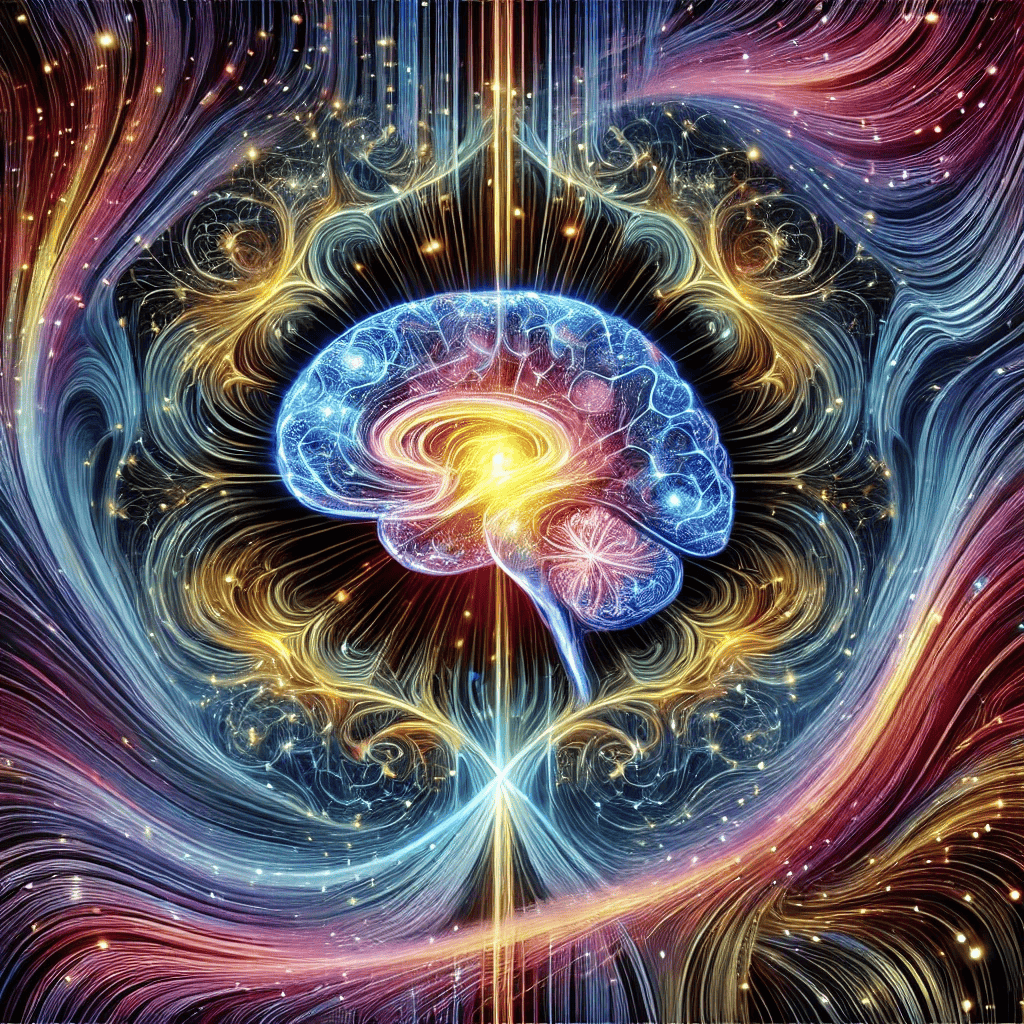
\includegraphics[width=0.8\textwidth]{cover.png}

    \caption{Cover art for Energetically Coherent Computation}
\end{figure}

\vspace{1cm}

\textit{This book was developed with significant reliance on advanced Large Language Models (LLMs), including Flux AI™, ChatGPT® and DALL·E® by OpenAI and Claude™ by Anthropic. These tools were instrumental in refining ideas, drafting and editing content, and even exploring and formulating mathematical models. While the core concepts and overarching framework remain my own, the collaborative nature of this work with LLMs has greatly shaped its structure and expression. Readers should understand this book as both an individual effort and a product of ongoing engagement with these transformative technologies.}

\vspace{2cm}

This work aims to establish a novel framework for understanding consciousness through an interdisciplinary synthesis spanning cognitive science, physics, and philosophy of mind. While computational approaches have proven remarkably successful in explaining many aspects of cognition, they face persistent challenges in accounting for phenomenal consciousness - the subjective, qualitative aspects of conscious experience.

The approach taken here attempts to bridge physical and computational perspectives. This theoretical framework, while speculative, draws on rigorous analysis of how phenomenology can link with current scientific understanding of the brain and engages with consciousness across cultural and historical contexts. A guiding intuition for this work is that the fundamental mysteries facing physics, biology, and psychology - the nature of energy, life, and consciousness respectively - may represent different aspects of a deeper theoretical challenge.

This work presents Energetically Coherent Computation (ECC) as a theoretical framework bridging multiple approaches to consciousness, but several important limitations warrant acknowledgment. While the framework offers mathematical sophistication, establishing clear empirical tests for its core claims remains a crucial challenge. The development of novel experimental methods to measure and manipulate patterns of energetic coherence will be essential for validating the theory's predictions.

The emphasis on energetic coherence should not be interpreted as dismissing the importance of neural computation. Rather than rejecting computational approaches, ECC suggests that computation alone cannot fully account for consciousness without considering its physical implementation through coherent energy dynamics. The framework aims to complement rather than replace computational understanding of neural processes.

The goal of this work is to suggest new ways of conceptualizing consciousness that bridge physical and experiential approaches while remaining open to refinement through future research. Readers are encouraged to approach these ideas critically while considering how they might be tested and developed through rigorous scientific investigation. Limitations notwithstanding, ECC offers valuable theoretical tools for understanding consciousness as simultaneously physical and experiential, suggesting productive directions for future research across multiple disciplines.

ECC aligns with Anil Seth's focus on addressing the "real" problem of consciousness - developing precise understanding of how phenomenology can be systematically influenced and controlled - rather than attempting to resolve the metaphysical challenges posed by the hard problem. As Phillip Goff argues, just as Maxwell advanced physics by assuming electromagnetic forces as fundamental while studying their behavior, consciousness research might progress by taking phenomenal experience as a basic feature of (of some part of) reality while investigating its organization and dynamics.

This pragmatic orientation acknowledges Thomas Nagel's fundamental insight about the apparent irreconcilability between first-person conscious experience and third-person scientific description. The "view from nowhere" that science attempts to achieve may be fundamentally incapable of capturing the subjective, qualitative aspects of consciousness. Rather than trying to bridge this explanatory gap, ECC focuses on understanding how physical patterns of energetic coherence relate to and influence conscious states while accepting the irreducibility of first-person experience.

By examining specific mechanisms through which patterns of energetic coherence shape conscious experience, ECC provides tools for addressing Seth's "real" problem - understanding consciousness well enough to enable precise control of phenomenal states. This creates opportunities for empirical investigation and potential therapeutic applications without requiring resolution of the deeper philosophical tensions Nagel identified between subjective and objective perspectives. The framework thus maintains scientific tractability while acknowledging the limitations of third-person approaches to understanding consciousness.

This approach suggests that progress in consciousness research may come not from trying to reduce phenomenal experience to physical description, but from developing increasingly sophisticated understanding of how physical processes and conscious experiences relate to and influence each other while remaining fundamentally distinct modes of reality. Just as physics advances without fully resolving questions about the ultimate nature of energy or matter, consciousness research can develop meaningful insights about the dynamics and control of experience while accepting certain philosophical limitations as fundamental rather than provisional.

As mentioned above, this work has been done with heavy use of modern large language models (LLMs) like Claude's Sonnet and ChatGPT's 4o. As of the 0.3.0 release, the references used in this document are still being revised for veracity (do they exist?) and fidelity (do they connect to the main text?). The text itself is also under revision - it presents a lot redundancy throughout and some contradictions between sections. Furthermore, not all sentences fully represent the views of the main author or may yet be misconstrued. A lot of (full time) work is still required to get this manuscript up to high academic standards. Thus, we advise the reader to engage with the text as a work in progress (a roadmap of sorts, more than a finished product) until a first edition is released. Pull requests and critiques are welcome on the \href{https://github.com/bobaseb/energetically-coherent-computation}{Github page}.

\section*{\phantom{Part II Abstract}}
\h{Abstract}

This book introduces Energetically Coherent Computation (ECC), a novel theoretical framework that reconceptualizes consciousness as emerging from coherent energy flows within biological systems rather than from abstract computation or symbolic manipulation. ECC represents a significant departure from traditional cognitive models by positioning consciousness as an emergent property of dynamically organized energy dynamics that span multiple scales—from molecular interactions and protein states to regional brain waves and global neural coherence. This physically grounded approach addresses fundamental challenges in cognitive science, including the symbol grounding problem, the unity of consciousness, and the relationship between physical and experiential properties.

The framework is built upon several key theoretical innovations. First, it proposes that consciousness requires specific forms of energetic coherence maintained through biological structures, particularly through astrocytic networks and the cortical neuropil. Second, it suggests that conscious states are shaped by unique transcriptomic profiles that create region-specific "alphabets" of possible energetic configurations. Third, it introduces the concept of "neural light cones" that define the causal boundaries of conscious integration. These elements work together to create a dynamically stable, unified field of consciousness that remains coherent while adapting to changing conditions.

\begin{figure}[h]
    \centering
    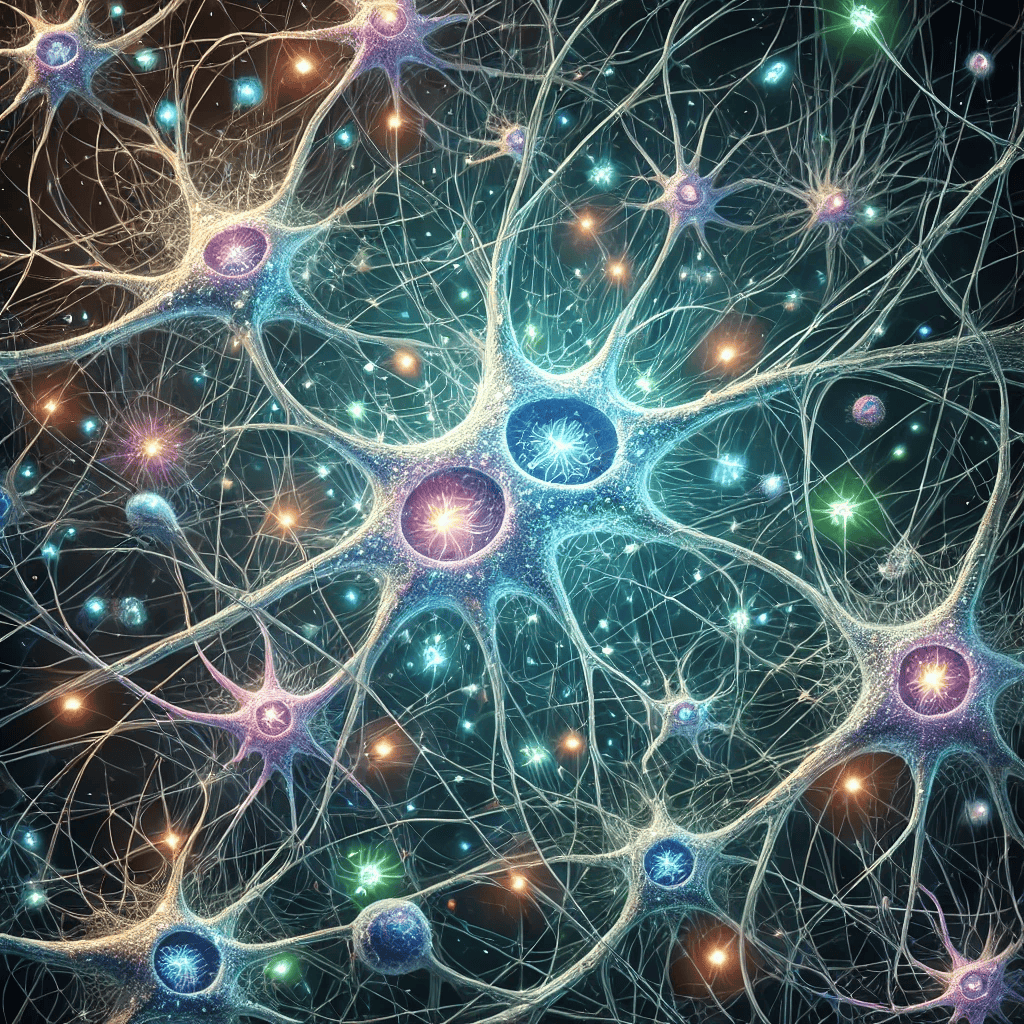
\includegraphics[width=0.8\textwidth]{astrocytes.png}

    \caption{Astrocytic Syncytia}
\end{figure}

Mathematically, ECC employs sophisticated formal tools to describe how local energy dynamics integrate into global conscious states. These include sheaf theory for modeling local-to-global coherence, the Jacobian of the stress-energy tensor for analyzing energy flows and their interactions, and principles of mutual recursion and triangulation for maintaining stability across scales. The framework also incorporates thermal noise as a boundary condition that shapes the scope and structure of conscious states, suggesting how background energy fluctuations contribute to conscious experience.

The theory offers novel interpretations of various psychological phenomena. It frames free will as the direct experience of enacting change through coherent energy flows, explains abstract thinking as a special case of conscious processing that requires active maintenance of ungrounded placeholders, and reinterprets perceptual phenomena like visual snow as manifestations of fundamental energy dynamics. Additionally, ECC provides insights into the nature of emotions, pain, and other subjective experiences by grounding them in specific patterns of energetic coherence.

ECC has significant implications for multiple fields, including neuroscience, artificial intelligence, philosophy of mind, and even anthropology. It suggests specific requirements for consciousness that go beyond computation alone, indicating why consciousness might be limited to biological systems or specially designed artificial systems that can achieve similar forms of energetic coherence. The framework also offers testable predictions about the relationship between energy dynamics and conscious experience, particularly through research on brain organoids and neuromorphic computing.

Through its integration of physical, biological, and mathematical principles, ECC provides a comprehensive framework for understanding consciousness that bridges phenomenology and neuroscience. By grounding conscious experience in the physical reality of the brain's continuous, multi-layered energy flows while maintaining mathematical rigor, it offers a promising direction for future research into the foundations of consciousness. The theory's emphasis on energetic coherence and physical embodiment represents a significant contribution to ongoing debates about the nature of mind, experience, and consciousness.

\section*{\phantom{Part III Foundations and Core Concepts}}
\h{Foundations and Core Concepts}

\section{Introduction}

\begin{refsection}[references/0001_1_foundations.bib]

The study of consciousness occupies a unique position at the intersection of neuroscience, philosophy, and physics. Traditional approaches have often treated consciousness as fundamentally computational - a series of information processing steps that could theoretically be implemented in any suitable substrate \cite{dennett1993consciousness}. However, this view struggles to account for several core aspects of conscious experience, including the unity of consciousness, the richness of qualia, and the grounding of mental representations in physical reality \cite{block1995confusion}.

This work introduces Energetically Coherent Computation (ECC), a novel framework that reconceptualizes consciousness as emerging from coherent energy flows within biological systems. Rather than reducing consciousness to abstract computation, ECC grounds it in the continuous, physically embodied dynamics of neural and glial networks. This approach synthesizes insights from multiple disciplines: from physics, it adopts concepts of field theories and thermodynamics \cite{prigogine2018order}; from neuroscience, it incorporates findings about astrocytic networks and transcriptomic diversity \cite{Giaume2010,Hawrylycz2012}; from philosophy, it engages with questions of embodiment and the nature of experience \cite{varela1991embodied}; and from biology, it considers how consciousness shapes and is shaped by living systems \cite{maturana1991autopoiesis}.

Central to ECC is the idea that consciousness requires more than information processing - it demands specific forms of energetic coherence typically found only in biological systems \cite{margulis2001conscious}. This coherence emerges from the dynamic interplay of multiple scales, from molecular interactions to regional brain dynamics, creating a stable yet flexible field that supports conscious experience \cite{thompson2010mind}. This perspective aligns with recent work suggesting that consciousness cannot be reduced to purely computational processes \cite{seth2024conscious}.

A key insight of ECC is that consciousness emerges from what we might call a rich alphabet of energetic states, shaped by the unique transcriptomic profiles of different brain regions. Unlike binary digital systems, biological systems employ a vastly more complex set of possible states, encoded in the diverse molecular and cellular configurations that characterize neural tissue \cite{levin2019computational}. This rich alphabet allows for the nuanced, context-sensitive representations that characterize conscious experience \cite{seth2021being,juarrero2023context}.

The framework extends beyond traditional theories of consciousness in several important ways. Where integrated information theory and global workspace theory emphasize information processing \cite{tononi2015consciousness,Baars2019}, ECC grounds consciousness in the physical reality of energy flows and their coherent organization. This grounding helps address longstanding problems in consciousness studies, including the symbol grounding problem and the hard problem of consciousness \cite{harnad1990symbol,chalmers1997conscious}. While ECC does not claim to solve the hard problem entirely - indeed, it suggests that some aspects of conscious experience may remain irreducible to third-person description \cite{nagel1980like,nagel1989view} - it provides a framework for understanding how consciousness emerges from physical systems in a way that respects both its subjective character and its basis in biological reality.

This approach represents a significant departure from traditional cognitive models, drawing inspiration from earlier work on self-reference and emergent meaning \cite{hofstadter1999godel}, dissipative structures \cite{prigogine2018order}, and biological autonomy \cite{bateson2000steps}. By integrating these perspectives with insights from modern neuroscience and philosophy of mind, ECC offers a novel framework for understanding consciousness that bridges phenomenology and physical reality while maintaining scientific rigor.

\begin{figure}[h]
    \centering
    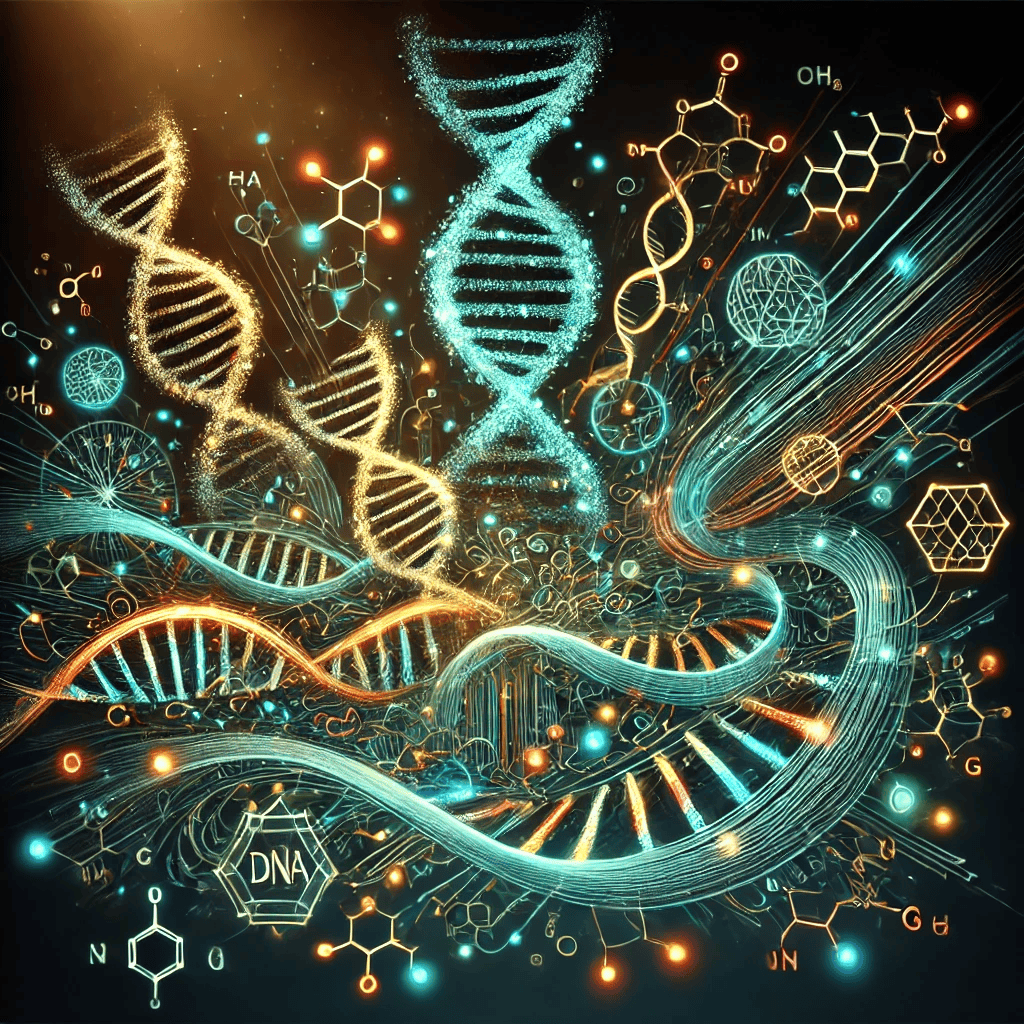
\includegraphics[width=0.8\textwidth]{transcriptomes.png}

    \caption{Transcriptomic profiles depend on a DNA -> RNA -> protein pipeline}
\end{figure}

The implications of ECC extend beyond theoretical neuroscience into practical domains including artificial intelligence and consciousness research. While current AI systems achieve remarkable computational feats, ECC suggests that conscious experience requires more than information processing alone - it demands specific forms of energetic coherence typically found in biological systems \cite{thompson2010mind}. This insight has profound implications for the development of artificial consciousness, suggesting that truly conscious machines might require novel architectures that can sustain coherent energy dynamics similar to those found in biological brains \cite{seth2024conscious}.

ECC's framework provides new tools for understanding altered states of consciousness, mental illness, and the effects of psychoactive compounds. By focusing on the organization of energy flows rather than just neural firing patterns, we can better understand how consciousness can be disrupted or modified at multiple scales \cite{varela1991embodied}. The model helps explain why certain medical conditions affect consciousness globally while others produce more localized effects, based on how they impact the brain's capacity to maintain energetic coherence across different regions.

Of particular significance is ECC's treatment of thermal noise and thermodynamic constraints in conscious processing. Rather than viewing noise as merely a limiting factor, ECC suggests that thermal fluctuations play a constructive role in consciousness, helping to establish boundaries between conscious and unconscious processing while contributing to the brain's capacity for flexible, adaptive response \cite{prigogine2018order}. This perspective aligns with recent findings in neuroenergetics while providing a theoretical framework for understanding how the brain maintains conscious coherence despite ongoing thermal fluctuations \cite{Berndt2012}.

The approach taken in this work represents a form of speculative psychology, bridging empirical neuroscience and philosophical inquiry \cite{seth2021being}. While grounded in physical and biological reality, this approach allows us to explore theoretical possibilities that extend beyond current experimental capabilities. Such speculation is crucial for advancing our understanding of consciousness, as many aspects of conscious experience remain difficult or impossible to measure directly with current technologies \cite{block1995confusion}.

The framework employs mathematical tools to model how local energy dynamics integrate into globally coherent conscious states. These mathematical formalisms help capture how consciousness maintains unity across space and time while remaining dynamically responsive to changing conditions \cite{Bredon1997,Arnowitt2008}. Through these tools, ECC provides a rigorous way to understand how consciousness achieves both stability and flexibility, maintaining coherent experience even as it continuously adapts to new inputs and internal states.

A central theme that emerges throughout this work is the distinction between computational and non-computational aspects of consciousness. While ECC acknowledges the importance of information processing in neural systems, it suggests that consciousness requires something more: specifically organized energy flows that maintain coherence across multiple scales - below, within and above the cellular level \cite{margulis2001conscious}. This perspective helps resolve long-standing debates about the relationship between computation and consciousness \cite{dennett1993consciousness}, suggesting that while computation may be necessary for conscious processing, it is not sufficient. The physical substrate matters, not because of any mystical properties, but because consciousness depends on specific forms of energetic organization that typical computational systems cannot achieve.

This insight has particular relevance for the ongoing debate about artificial consciousness. While ECC does not rule out the possibility of machine consciousness entirely, it suggests that achieving it would require more than implementing the right algorithms \cite{block1995confusion}. Instead, artificial systems would need to replicate the specific forms of energetic coherence found in biological brains - a considerably more challenging engineering task that aligns with recent theoretical developments in consciousness studies (see \cite{tononi2015consciousness} for an information-based view).

The framework presented also has important implications for our understanding of biological evolution. Rather than viewing consciousness as a late addition to complex nervous systems, ECC suggests that basic forms of conscious experience might be present even in simple cellular systems that maintain appropriate forms of energetic coherence \cite{margulis2001conscious}. This aligns with emerging research in basal cognition and suggests that consciousness might be more fundamental to life than previously thought \cite{levin2019computational,Lyon2021}, while still maintaining clear distinctions between simpler and more complex forms of conscious experience.

A significant advance offered by ECC is its treatment of the brain's rich alphabet - the diverse range of energetic states made possible by region-specific transcriptomic profiles \cite{Tasic2018}. This concept helps explain how the brain achieves both the precision and flexibility characteristic of conscious experience. Unlike digital systems restricted to binary states, biological neural systems can access a vast repertoire of energetically distinct states, allowing for nuanced representations that maintain sharp categorical boundaries while supporting continuous gradations within categories \cite{Freedman2011}.

The framework also offers new insights into the relationship between consciousness and thermodynamic processes. Rather than viewing thermal noise solely as a source of disruption, ECC suggests that it plays a constructive role in conscious processing, helping to establish natural boundaries between conscious and unconscious states while contributing to the brain's adaptive capabilities \cite{prigogine2018order}. This perspective aligns consciousness with fundamental physical principles while explaining how biological systems achieve the remarkable feat of maintaining stable, coherent experience in the face of constant molecular fluctuations.

Central to our argument is the role of astrocytic networks and their influence on conscious processing. While much of neuroscience has focused on neurons as the primary substrate of consciousness, ECC suggests that astrocytes play a crucial role in maintaining the coherent energy fields necessary for conscious experience \cite{Bazargani2016}. This emphasis on glial contributions helps explain how the brain achieves both the stability and flexibility required for consciousness, while suggesting new directions for experimental investigation.

The empirical implications of ECC extend beyond theoretical neuroscience into practical domains of medicine and experimental psychology. By framing consciousness in terms of energetic coherence, ECC suggests new approaches to understanding and treating disorders of consciousness (cf. \cite{tononi2015consciousness}). Traditional neurological approaches have often focused on patterns of neural firing or neurotransmitter levels, but ECC suggests that disruptions to consciousness might better be understood as perturbations in the brain's capacity to maintain coherent energy fields.

Moreover, ECC provides a fresh framework for investigating the relationship between consciousness and sleep. Unlike death, which represents a permanent disruption of energetic coherence, sleep involves a controlled modulation of coherent states. This distinction helps explain why consciousness can be readily restored after sleep but not after death, while also suggesting new approaches to understanding sleep disorders and altered states of consciousness \cite{Dittrich2010}. The framework's treatment of thermal noise and energetic boundaries proves particularly valuable here, offering insights into how the brain maintains different levels of conscious awareness across sleep-wake cycles \cite{prigogine2018order}.

Of particular relevance to current research in cognitive neuroscience is ECC's approach to the neural correlates of consciousness. Rather than seeking discrete neural signatures of conscious experience, ECC suggests that we should look for patterns of energetic coherence across multiple scales. This implies that consciousness might be better understood through new experimental techniques that can measure energy flows and field-like properties of neural tissue, rather than focusing solely on action potentials or metabolic activity.

The philosophical implications of ECC are equally significant. By grounding consciousness in physical energy flows while preserving its irreducible qualitative aspects \cite{nagel1980like}, ECC offers a novel perspective on the mind-body problem. Unlike traditional physicalist accounts that risk eliminating the subjective character of experience \cite{dennett1993consciousness}, or dualist approaches that struggle to explain mind-body interaction \cite{chalmers1997conscious}, ECC suggests how consciousness can be fundamentally physical while maintaining its distinctive phenomenological features \cite{block1995confusion}.

Perhaps most significantly, ECC provides new insights into the nature of free will and agency. Rather than viewing free will as incompatible with physical causation, ECC suggests (a compatibilist view, \cite{Beebee2002}) that conscious agency emerges naturally from the brain's capacity to maintain coherent, self-organizing energy fields. This perspective sees conscious decisions not as computations carried out by neural circuits, but as dynamic reorganizations of energetic coherence across the cortical sheet.

The implications for artificial intelligence research are particularly profound. While current AI systems have achieved remarkable success in specific domains, ECC suggests that achieving genuine consciousness in artificial systems would require more than sophisticated self-referential algorithms or neural network architectures \cite{hofstadter1999godel,Rumelhart1986}. Instead, it would demand creating physical systems capable of sustaining the specific forms of energetic coherence found in biological brains implemented at the cellular level \cite{margulis2001conscious}.

The mathematical formalism developed in this work provides precise tools for modeling how local energy dynamics integrate into globally coherent conscious states. These mathematical structures are not merely descriptive but capture essential features of how consciousness emerges from physical systems. The use of formal mathematical approaches helps explain how local coherence in different brain regions can be integrated to form a unified conscious field, while energy tensor formalism provides a way to understand how energy flows are organized and maintained across multiple scales.

This formal approach leads to specific, testable predictions about the relationship between energy dynamics and conscious experience. For instance, ECC predicts that disruptions to astrocytic networks should have specific, measurable effects on consciousness that differ from disruptions to neural firing patterns alone. Similarly, the framework suggests that conscious processing should show distinctive patterns of energy organization that differ from unconscious neural activity.

Through careful attention to boundary conditions, ECC provides new insight into the limits of conscious experience. The framework suggests that consciousness emerges only when cellular systems achieve sufficient coherence to maintain stable yet dynamic energy states \cite{maturana1991autopoiesis}. This explains both why consciousness appears limited to certain biological systems and how it can support such remarkable flexibility within those constraints.

The interaction between cellular and network-level processes takes on new significance through ECC's lens. Rather than treating these as separate levels of organization, the framework shows how they represent different scales of coherent energy dynamics. This multi-scale integration helps explain how consciousness can maintain both local specificity and global unity, a feature that has challenged both biopsychist and biological naturalist accounts.

The synthesis of biopsychist and biological naturalist perspectives in ECC ultimately points toward a fundamental insight: consciousness cannot be reduced to computational processes alone, regardless of their complexity \cite{seth2024conscious}. This departure from computational theories of mind emerges naturally from ECC's emphasis on physical dynamics and energetic coherence in biological systems \cite{thompson2010mind}.

The energetic requirements for consciousness, as revealed through ECC's analysis of cellular and systemic organization, demonstrate why computation alone proves insufficient for generating conscious experience \cite{piccinini2013neural}. While computational processes can simulate or model aspects of consciousness, they cannot replicate the fundamental coherence that emerges from continuous, physically-grounded energy dynamics. This insight helps resolve longstanding debates about the possibility of machine consciousness while explaining why biological systems remain uniquely capable of supporting conscious experience \cite{margulis2001conscious}.

The framework's emphasis on physical implementation extends beyond traditional arguments about substrate dependence \cite{polger2016multiple}. Rather than simply claiming that consciousness requires particular physical structures, ECC demonstrates how specific patterns of energetic coherence, maintained through sophisticated biological machinery, create the conditions necessary for conscious experience. These patterns cannot be reduced to abstract information processing but require continuous, physically-grounded processes that integrate multiple scales of biological organization \cite{maturana1991autopoiesis}.

In the sections that follow, we develop these ideas in detail, moving from theoretical foundations through specific applications to broader implications. The first section establishes the physical and mathematical framework of ECC, followed by explorations of specific phenomena in consciousness, including the unity of experience, the nature of qualia, and the binding problem. The final sections explore practical implications for fields ranging from medicine to artificial intelligence to new perspectives on anthropology.

ECC presents a distinctive philosophical approach to consciousness that departs significantly from traditional computationalist views while maintaining a firmly physicalist stance. At its core, ECC posits that consciousness emerges not from abstract information processing or symbolic manipulation, but from coherent energy flows within biological systems. This philosophical framework challenges both classical functionalism and computational theories of mind by emphasizing the irreducible role of physical embodiment and energetic dynamics in conscious experience \cite{thompson2010mind}. Through careful analysis of energetic coherence patterns and their relationship to conscious states, ECC offers novel perspectives on longstanding questions in philosophy of mind, including the symbol grounding problem, the nature of qualia, and the relationship between physical and experiential properties.

\section{Biopsychism and Biological Naturalism}

ECC aligns closely with both biopsychist perspectives and biological naturalism, though it offers distinct contributions to each framework through its emphasis on energetic coherence and cellular organization. Like biopsychism, ECC locates consciousness at the cellular level, suggesting that conscious experience emerges from the fundamental properties of living systems \cite{edwards2005consciousness, shapiro2007bacteria}. However, ECC specifies that this emergence requires particular forms of energetic coherence and organization that are characteristic of biological systems, especially neural and glial networks.

From biological naturalism, ECC inherits the view that consciousness is irreducibly grounded in biological processes \cite{searle2017biological}. However, while traditional biological naturalism focuses primarily on neural systems, ECC expands this view to encompass broader cellular and energetic dynamics. This expansion allows ECC to bridge the gap between simpler cellular awareness and complex conscious experience through its framework of energetic coherence \cite{van2006principles}.

The cellular foundations of consciousness in ECC parallel biopsychist insights, but with crucial distinctions. While both approaches recognize consciousness at the cellular level \cite{lyon2015cognitive}, ECC emphasizes that these cellular processes must achieve specific forms of energetic coherence to support consciousness. This requirement distinguishes ECC from broader forms of biopsychism that might attribute consciousness to all cellular activity without qualification \cite{margulis2000life}.

The energetic organization principles of ECC provide a mechanistic framework for understanding how biological systems generate conscious experience. While biological naturalism emphasizes the biological basis of consciousness \cite{searle1992rediscovery}, ECC specifies that the critical biological features are those that enable coherent energy flows and stable feedback systems. This focus on energetic organization provides concrete mechanisms for understanding how biological systems generate conscious experience, moving beyond both general biopsychist claims and traditional biological naturalist approaches \cite{thompson2010mind}.

ECC suggests that complex consciousness emerges from the integration of cellular-level coherence into broader, stable fields through mechanisms like astrocytic syncytia and transcriptomic profiles. This multi-level integration explains how simple cellular awareness can scale to complex conscious experience while maintaining the biological grounding emphasized by both biopsychism and biological naturalism \cite{godfrey2016other}.

Within an evolutionary context, ECC's framework provides an account that aligns with both perspectives while offering additional specificity \cite{varela1997patterns}. It suggests that consciousness evolved as biological systems developed increasingly sophisticated mechanisms for maintaining energetic coherence, beginning with cellular processes and culminating in the complex neural systems of modern organisms \cite{deacon2011incomplete}.

Through this synthesis, ECC offers a framework that preserves the key insights of both biopsychism and biological naturalism while providing a more specific mechanism - energetic coherence - for understanding how biological systems generate conscious experience. This approach suggests that consciousness is neither a universal property of all biological systems nor limited to neural activity alone, but rather emerges from specific forms of energetically coherent biological organization \cite{clark2010supersizing}.

\begin{figure}[h]
    \centering
    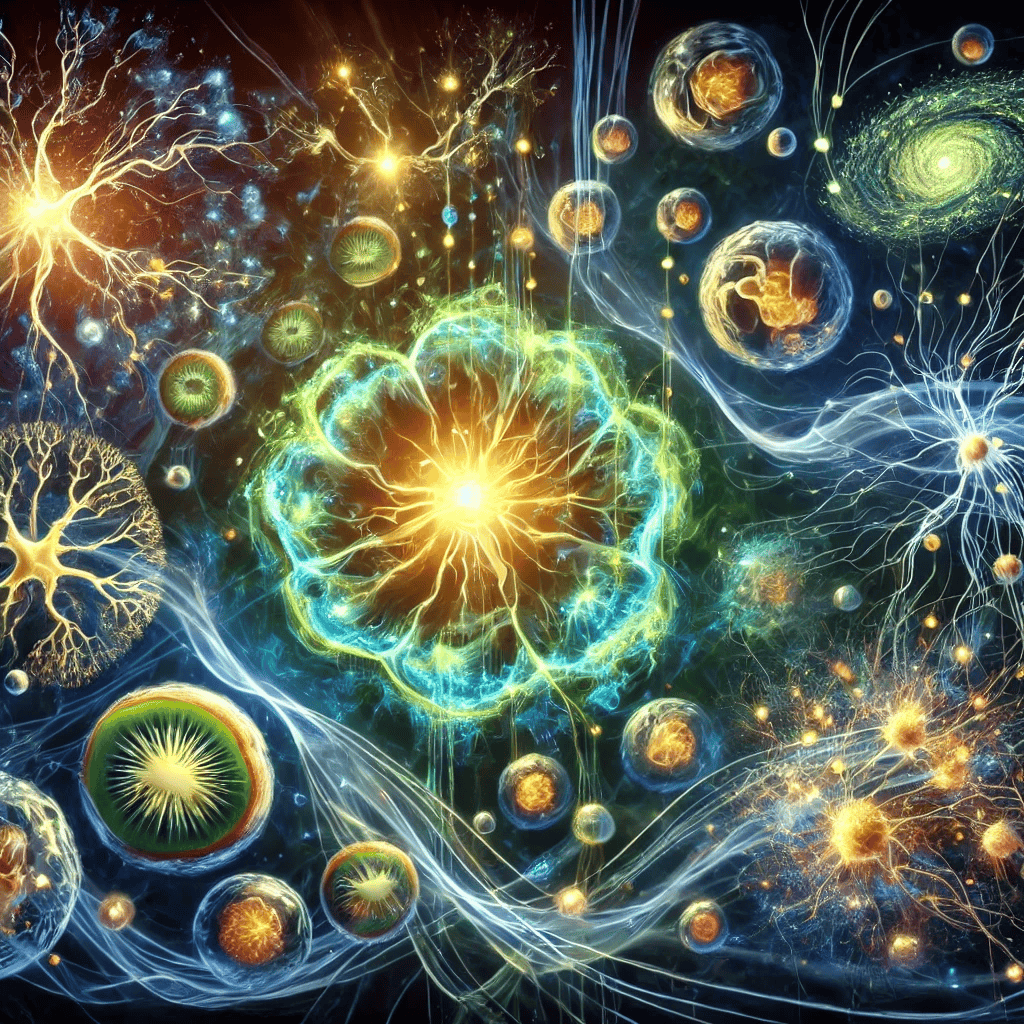
\includegraphics[width=0.8\textwidth]{conscious_cells.png}

    \caption{Biopsychism - cells are conscious}
\end{figure}

The relationship between cellular organization and conscious experience takes on particular significance in ECC's framework. Through specific patterns of energetic coherence, cellular networks achieve forms of integration that transcend simple aggregation \cite{lyon2015cognitive}. These patterns emerge through the interplay of membrane dynamics, ion gradients, and bioelectric fields that characterize living systems. Unlike traditional biological naturalism, which might treat these features as mere implementation details \cite{searle2017biological}, ECC positions them as fundamental to the generation of conscious states.

The role of transcriptomic profiles in shaping conscious capacity represents another crucial advance in ECC's synthesis \cite{Tasic2018,Hawrylycz2012}. Different cell populations maintain distinct molecular configurations that enable particular forms of energetic coherence \cite{shapiro2007bacteria}. This molecular diversity creates what ECC terms a rich alphabet of possible conscious states, explaining both how consciousness can maintain stability and how it can support sophisticated information processing. This perspective bridges the seeming gap between cellular-level awareness and complex conscious experience \cite{van2006principles}.

ECC's treatment of astrocytic networks provides a concrete example of how its framework extends beyond both biopsychism and biological naturalism. These networks create continuous domains of coordinated activity through gap junctions and calcium waves, establishing coherent fields that span multiple cellular populations \cite{edwards2005consciousness}. This mechanism demonstrates how consciousness can emerge at scales beyond individual cells while remaining grounded in cellular processes \cite{thompson2010mind}.

The framework particularly illuminates the relationship between metabolism and consciousness. Where traditional approaches might treat energy management as merely supportive of conscious processing \cite{searle1992rediscovery}, ECC suggests that specific patterns of energetic organization are constitutive of consciousness itself. This helps explain why consciousness requires such sophisticated cellular machinery while avoiding claims that all metabolic processes generate consciousness \cite{margulis2000life}.

Through careful attention to boundary conditions, ECC provides new insight into the limits of conscious experience. The framework suggests that consciousness emerges only when cellular systems achieve sufficient coherence to maintain stable yet dynamic energy states \cite{varela1997patterns}. This explains both why consciousness appears limited to certain biological systems and how it can support such remarkable flexibility within those constraints \cite{godfrey2016other}.

The interaction between cellular and network-level processes takes on new significance through ECC's lens. Rather than treating these as separate levels of organization, the framework shows how they represent different scales of coherent energy dynamics \cite{lyon2015cognitive}. This multi-scale integration helps explain how consciousness can maintain both local specificity and global unity, a feature that has challenged both biopsychist and biological naturalist accounts \cite{clark2010supersizing}.

This theoretical synthesis has important practical implications for understanding disorders of consciousness and potential therapeutic interventions. By identifying specific mechanisms through which conscious states emerge from cellular processes \cite{deacon2011incomplete}, ECC suggests new approaches to treating conditions that affect consciousness. This demonstrates how the framework moves beyond philosophical positions to generate concrete insights for medical applications \cite{thompson2010mind}.

The synthesis of biopsychist and biological naturalist perspectives in ECC ultimately points toward a fundamental insight: consciousness cannot be reduced to computational processes alone, regardless of their complexity \cite{thompson2010mind}. This departure from computational theories of mind emerges naturally from ECC's emphasis on physical dynamics and energetic coherence in biological systems \cite{searle2017biological}.

The energetic requirements for consciousness, as revealed through ECC's analysis of cellular and systemic organization, demonstrate why computation alone proves insufficient for generating conscious experience \cite{varela1997patterns}. While computational processes can simulate or model aspects of consciousness, they cannot replicate the fundamental coherence that emerges from continuous, physically-grounded energy dynamics. This insight helps resolve longstanding debates about the possibility of machine consciousness while explaining why biological systems remain uniquely capable of supporting conscious experience \cite{lyon2015cognitive}.

The framework's emphasis on physical implementation extends beyond traditional arguments about substrate dependence \cite{edwards2005consciousness,polger2016multiple}. Rather than simply claiming that consciousness requires particular physical structures, ECC demonstrates how specific patterns of energetic coherence, maintained through sophisticated biological machinery, create the conditions necessary for conscious experience \cite{shapiro2007bacteria}. These patterns cannot be reduced to abstract information processing but require continuous, physically-grounded processes that integrate multiple scales of biological organization \cite{van2006principles}.

This non-computational nature of consciousness becomes particularly evident when examining how biological systems achieve coherent integration across different scales \cite{margulis2000life}. Unlike digital computers that maintain sharp boundaries between processing elements, conscious systems operate through continuous fields of influence that span multiple levels of organization. The resulting integration cannot be achieved through discrete computational steps but requires physical processes that maintain coherence through direct energetic interaction \cite{godfrey2016other}.

\section{Consciousness as Non-computational}

ECC's proposal represents a distinctive philosophical approach to consciousness that diverges from traditional computationalist views while maintaining a firmly physicalist stance \cite{piccinini2020neurocognitive}. At its core, ECC posits that consciousness emerges not from abstract information processing or symbolic manipulation, but from coherent energy flows within biological systems. This philosophical framework challenges both classical functionalism and computational theories of mind by emphasizing the irreducible role of physical embodiment and energetic dynamics in conscious experience \cite{thompson2001radical}.

ECC's philosophical commitments can be understood through three fundamental principles. First, consciousness requires specific forms of energetic coherence that cannot be reduced to computational processes alone \cite{van1995might}. Unlike traditional functionalist approaches that treat consciousness as substrate-independent, ECC argues that conscious experience is inherently tied to particular physical and energetic configurations, typically found in biological systems. Second, ECC maintains that consciousness operates through a rich alphabet of energetic states, shaped by transcriptomic profiles and molecular diversity, rather than through binary or discrete symbolic representations \cite{wheeler2005reconstructing}. Third, consciousness emerges as a field-like phenomenon characterized by continuous, dynamic coherence rather than discrete state transitions.

This philosophical stance positions ECC as a unique bridge between physicalist and emergentist views of consciousness \cite{jonas2001phenomenon}. While firmly grounded in physical processes, ECC suggests that conscious experience emerges from specific organizations of energy flows. Where the dynamics of said energy flows may admit a computational description, conscious experience itself cannot be captured by purely computational or mechanistic descriptions. This approach offers a novel solution to classical philosophical problems such as the symbol grounding problem \cite{harnad1990symbol} and the hard problem of consciousness \cite{chalmers1997conscious}, by rooting conscious experience in concrete, physically realized energy dynamics rather than abstract computational processes.

This physicalist yet non-computationalist approach has significant implications for several longstanding debates in philosophy of mind. First, regarding multiple realizability—a cornerstone of traditional functionalism—ECC takes a more constrained position \cite{piccinini2013neural, anderson2024physical}. While conscious states might be realizable in different physical substrates, ECC argues that these substrates must be capable of supporting specific types of energetic coherence and dynamic stability. This suggests that consciousness cannot be implemented in just any computational system, but requires materials and organizations capable of sustaining coherent energy flows similar to those found in biological brains \cite{van1995might}.

ECC's stance on the mind-body problem is particularly distinctive. Rather than treating consciousness as an emergent property of computational processes \cite{piccinini2020neurocognitive} or as a fundamental feature of all matter \cite{Goff2019}, ECC suggests that consciousness arises specifically from coherent energy dynamics within systems that maintain low-entropy, stable states. This view acknowledges the physical basis of consciousness while recognizing that not all physical systems—even those capable of complex information processing \cite{tononi2016integrated}—will necessarily give rise to conscious experience. The key distinction lies in a system's ability to achieve and maintain energetic coherence across multiple scales \cite{horst2011symbols}.

The framework also offers fresh insights into the nature of qualia or phenomenal experience. Instead of treating qualia as computational states or abstract representations \cite{bishop2009computers}, ECC grounds them in specific patterns of energetic coherence shaped by transcriptomic profiles and molecular diversity. This approach suggests that the qualitative aspects of conscious experience are neither mysterious nor epiphenomenal, but are direct manifestations of structured energy flows within biological systems \cite{noe2009out}. Such a view helps bridge the explanatory gap between physical processes and phenomenal experience by identifying consciousness with particular forms of energetic organization.

Perhaps most significantly, ECC's philosophical framework challenges us to rethink the relationship between function and implementation in conscious systems \cite{piccinini2013neural}. While traditional approaches have often treated these as separable—with function being abstractable from physical implementation—ECC suggests they are fundamentally intertwined when it comes to consciousness. The specific energetic dynamics that give rise to conscious experience cannot be separated from their physical realization without losing essential properties that make consciousness possible \cite{van1995might}. This represents a form of embodied functionalism that recognizes the inseparability of conscious functions from their physical instantiation.

This philosophical stance has profound implications for artificial consciousness and cognitive science. It suggests that creating conscious artificial systems would require not just implementing the right algorithms or information processing architecture \cite{searle1980minds} (cf. \cite{butlin2023consciousnessartificialintelligenceinsights}), but engineering physical systems capable of sustaining the specific types of energetic coherence found in biological brains. This moves beyond the traditional artificial intelligence paradigm of abstract computation toward a more biologically-inspired approach that emphasizes physical dynamics and energy flows \cite{dreyfus1992computers}.

ECC thus presents a philosophical framework that is at once physicalist and non-reductionist, acknowledging both the material basis of consciousness and the impossibility of reducing it to purely computational descriptions \cite{horst2011symbols}. It offers a middle path between eliminative materialism \cite{churchland1986neurophilosophy} and dualism \cite{chalmers1997conscious}, suggesting that consciousness is neither illusion nor magic, but rather a physical phenomenon requiring specific forms of energetic organization and coherence \cite{jonas2001phenomenon}.

The classical computational framework, articulated through universal machines \cite{turing1936computable} and formalized cognitive processes (e.g., \cite{marr1982vision}), has dominated functionalist accounts of mind \cite{putnam1988representation}. This computational paradigm suggests that any cognitive process can be understood as an algorithm operating on representations. As mentioned above, this framework faces fundamental challenges when applied to consciousness \cite{fodor2000mind}.

Not every natural process requires or admits computational description \cite{rosen1991life}. Just as digestion cannot be adequately characterized as information processing, and gravitational phenomena cannot be reduced to computation, conscious experience may emerge from physical dynamics that resist computational abstraction. This aligns with later skepticism about the computational theory of mind, particularly regarding the context-sensitivity and holistic nature of conscious thought \cite{gibson2014ecological}. The framework suggests that attempting to reduce consciousness to computation represents a category error - confusing the abstract map of computational description with the physical territory of conscious experience. Furthemore, though we accept that the energy flows that support consciousness may admit a computational description, they are not equivalent to them.

This perspective helps resolve certain paradoxes in functionalist theories of mind \cite{piccinini2020neurocognitive}. Rather than treating consciousness as substrate-independent computation, ECC suggests it emerges from specific patterns of energetic coherence that remain grounded in physical dynamics. This maintains functionalism's key insight about the importance of organization while avoiding what has been identified as "computational chauvinism" - the tendency to treat all cognitive processes as fundamentally computational \cite{bishop2009computers}. The framework indicates that while some mental processes may be computational in nature, consciousness itself requires physical dynamics that exceed purely computational description.

Traditional functionalism has become so intertwined with computational theory of mind that the two are often treated as inseparable \cite{piccinini2020neurocognitive}. However, ECC suggests a novel approach: a functionalism grounded in energetic coherence rather than abstract computation. This reformulation maintains functionalism's core insight—that mental states are defined by their functional roles—while departing from the assumption that these roles must be realized through computational processes \cite{van1995might}.

In this reconceptualization, mental functions are understood not as algorithmic operations (in an ontological sense, though they can be in an epistemological one) but as patterns of coherent energy flows within physically structured systems \cite{thompson2001radical}. Where traditional functionalism might describe perception as information processing, ECC might characterize it as the achievement and maintenance of specific energetic configurations that faithfully represent environmental stimuli \cite{gibson2014ecological}. Similarly, memory becomes not the storage and retrieval of symbolic information, but the stabilization and reactivation of particular energetic patterns within the brain's coherent field.

This \textit{energetic functionalism} differs crucially from computational functionalism in its treatment of implementation \cite{horst2011symbols}. While computational functionalism suggests that any substrate capable of implementing the right algorithms could support consciousness, energetic functionalism argues that conscious functions require specific physical conditions that enable coherent energy flows. The function cannot be abstracted from its physical realization because the very nature of the function—the maintenance of coherent, low-entropy states—depends on particular physical and energetic properties \cite{rosen1991life}.

This energetic functionalism differs crucially from computational functionalism in its treatment of implementation. While computational functionalism suggests that any substrate capable of implementing the right algorithms could support consciousness \cite{wheeler2010defense}, energetic functionalism argues that conscious functions require specific physical conditions that enable coherent energy flows. The function cannot be abstracted from its physical realization because the very nature of the function—the maintenance of coherent, low-entropy states—depends on particular physical and energetic properties \cite{nicholson2018everything,whitehead2010process}.

To recap, this reformulation addresses several longstanding challenges in functionalist theory \cite{polger2016multiple}. First, it offers a solution to the symbolic grounding problem by rooting mental functions in physically realized energy dynamics rather than abstract symbols. In ECC's energetic functionalism, meaning and representation are not arbitrary mappings requiring external grounding, but emerge directly from the brain's coherent energy states shaped by transcriptomic profiles and molecular diversity \cite{gillett2016reduction}. The rich alphabet of possible states provides an intrinsically grounded basis for representation without requiring computational abstraction.

Moreover, energetic functionalism provides new insights into the unity of consciousness—a phenomenon that has proven difficult to explain within traditional computational frameworks \cite{van1998dynamical}. Rather than requiring a central processor or global workspace \cite{Baars2013} to integrate discrete computational processes, ECC suggests that unity emerges naturally from the continuous, field-like properties of coherent energy flows \cite{McFadden2020}. The brain's capacity to maintain coherent states across multiple scales creates a unified conscious field without needing additional mechanisms to bind separate processes together \cite{thompson2011living}.

This approach also offers a more nuanced view of multiple realizability. While maintaining that conscious functions could potentially be realized in different physical substrates, energetic functionalism argues that these substrates must be capable of supporting specific types of energetic coherence. This suggests a constrained form of multiple realizability where conscious functions are replicable only in systems that can achieve and maintain the necessary patterns of energy flow. Such systems might include both biological brains and specially engineered artificial structures, but would exclude traditional digital computers that operate through discrete state transitions \cite{wheeler2010defense}.

Energetic functionalism also provides new perspectives on the relationship between consciousness and physical implementation \cite{mossio2015biological}. Unlike computational functionalism, which treats implementation details as largely irrelevant to mental functions, ECC suggests that certain physical properties—particularly those that enable coherent energy flows—are essential to conscious functions. This doesn't reduce mental states to physical states in a simple type-identity fashion, but rather suggests that conscious functions require specific classes of physical organization that support energetic coherence \cite{dupre2012processes}.

This view has important implications for artificial consciousness. Rather than focusing on replicating computational algorithms, the development of conscious artificial systems would require engineering physical substrates capable of supporting coherent energy dynamics similar to those found in biological brains \cite{chemero2013radical}. This might involve creating new kinds of materials and architectures that can maintain low-entropy, coherent states across multiple scales. The goal would not be to simulate consciousness computationally, but to create physical systems that can achieve and maintain the kinds of energetic coherence necessary for conscious experience \cite{hutto2012radicalizing}.

The shift from computational to energetic functionalism suggests a novel approach to understanding the nature of consciousness and its relationship to physical systems \cite{nicholson2018everything}. This reconceptualization naturally leads us to consider how this view relates to traditional debates about type and token identity theories in the philosophy of mind. While traditional type identity theory suggests a one-to-one correspondence between mental and physical states, and token identity theory allows for multiple physical realizations of the same mental state, ECC's approach suggests a more nuanced view based on classes of energetic coherence \cite{gillett2016reduction}.

\section{Type/Token Identity Theory}

TODO: resume first pass on refs here

The relationship between ECC and classical identity theories presents an intriguing synthesis that moves beyond traditional type-type and token-token identity accounts of consciousness \cite{polger2009evaluating}. While type identity theory posits strict one-to-one correspondences between mental and physical states, and token identity theory allows for multiple physical realizations of the same mental state \cite{bechtel1999multiple}, ECC suggests a more nuanced position centered on patterns of energetic coherence. This framework might be termed coherence-class identity theory, where conscious states are identical with specific classes of energetically coherent physical states.

In traditional type identity theory, each type of mental state is identical with a specific type of physical state \cite{place1956is}. ECC modifies this view by suggesting that conscious states are identical not with specific physical configurations per se, but with patterns of energetic coherence that might be realized through different but physically constrained implementations \cite{shapiro2000multiple}. Unlike token identity theory, which allows for arbitrary physical realizations, ECC argues that these implementations must support specific types of energy dynamics shaped by transcriptomic profiles and molecular diversity.

This position maintains the physicalist commitments of identity theory while acknowledging that consciousness requires more than just the right physical structure—it requires the right kind of energetic organization and coherence \cite{richardson2008multiple}. The "types" in ECC's framework are defined not by specific physical configurations but by classes of energy dynamics that can support conscious experience. This allows for a limited form of multiple realizability while still maintaining that consciousness is fundamentally a physical phenomenon \cite{kim1992multiple}.

This coherence-class approach helps resolve several traditional problems faced by both type and token identity theories \cite{lewis1966argument}. Where classical type identity theory struggles to account for the apparent multiple realizability of mental states, and token identity theory risks making consciousness too abstract by allowing any suitable physical implementation, ECC's framework provides principled constraints on what kinds of physical systems could support consciousness. These constraints are based not on specific physical structures but on the capacity to maintain coherent energy dynamics across multiple scales \cite{wilson2001two}.

The framework is particularly illuminating when considering the relationship between brain structure and conscious experience \cite{block1972what}. Different brain regions with similar transcriptomic profiles might achieve the same type of energetic coherence despite variations in their detailed physical structure. Conversely, regions with different profiles might support distinct types of conscious experience through their unique patterns of energy organization. This explains how the brain can maintain stable conscious states despite continuous molecular turnover and neural plasticity—it is the pattern of energetic coherence, rather than the specific physical implementation, that remains constant \cite{polger2009evaluating}.

This view also has important implications for understanding the unity of consciousness \cite{craver2007explaining}. Traditional identity theories struggle to explain how diverse physical states across the brain combine to create unified conscious experience. ECC suggests that unity emerges from the brain's capacity to maintain coherent energy dynamics across multiple regions, creating a unified field of consciousness through patterns of energetic organization rather than through identity with specific physical states. This coherent field allows for both the integration and differentiation that characterize conscious experience \cite{feigl1967mental}.

ECC's coherence-class identity theory also provides new insights into the relationship between physical and phenomenal properties of consciousness \cite{place1956is}. Rather than attempting to identify qualia directly with physical states or treating them as emergent properties of information processing, this framework suggests that qualitative experiences are identical with specific patterns of energetic coherence \cite{smart1959sensations}. These patterns, shaped by transcriptomic profiles and molecular diversity, provide the rich alphabet necessary for the varied and nuanced character of conscious experience while maintaining its fundamentally physical nature.

This approach helps bridge the explanatory gap between physical and phenomenal properties without reducing one to the other \cite{lewis1966argument}. The qualitative aspects of consciousness are neither mysterious additions to physical reality nor mere computational abstractions, but rather are identical with particular classes of energetically coherent states. This preserves the physicalist foundations of identity theory while accounting for the distinctive phenomenal character of conscious experience \cite{block1972what}.

The coherence-class framework also offers novel solutions to problems that have plagued traditional identity theories \cite{shapiro2000multiple}. For instance, the issue of multiple realizability, which has been a persistent challenge for type identity theory, takes on a different character when viewed through the lens of energetic coherence. While different physical implementations might support conscious experience, they must all achieve specific patterns of energetic organization—a constraint that provides a principled basis for limiting the scope of multiple realizability \cite{bechtel1999multiple}.

Moreover, this view helps explain why certain physical states give rise to particular phenomenal experiences \cite{kim1992multiple}. The connection between physical and experiential properties is not arbitrary but is grounded in the specific patterns of energetic coherence that different brain states can achieve. This helps explain both the regularity of conscious experience—why similar physical states reliably produce similar experiences—and its variability, as different patterns of energetic coherence can support different types of conscious states \cite{richardson2008multiple}.

The relationship between local and global aspects of consciousness also becomes clearer through this framework \cite{wilson2001two}. While traditional identity theories often struggle to explain how localized neural activity contributes to unified conscious experience, ECC's coherence-class approach shows how local patterns of energetic coherence can integrate into global conscious states through principled physical mechanisms. This integration is not merely additive but involves the maintenance of coherent energy dynamics across multiple scales \cite{polger2009evaluating}.

This theoretical framework also has important implications for understanding the temporal dynamics of consciousness \cite{craver2007explaining}. Rather than treating conscious states as static physical configurations, ECC emphasizes the importance of dynamic patterns of energetic coherence that unfold over time. This temporal aspect helps explain both the continuity of conscious experience and its capacity for rapid change, as patterns of energetic coherence can maintain stability while remaining responsive to new inputs and internal dynamics \cite{feigl1967mental}.

The implications of coherence-class identity theory extend beyond theoretical concerns to practical questions about consciousness research and intervention \cite{richardson2008multiple}. By identifying conscious states with specific patterns of energetic coherence, the framework suggests new approaches to measuring and manipulating consciousness. Rather than focusing solely on neural firing patterns or neurotransmitter levels, this view suggests that understanding consciousness requires tracking patterns of energetic organization across multiple scales \cite{bechtel1999multiple}.

This reconceptualization also has important implications for how we understand disorders of consciousness \cite{shapiro2000multiple}. Rather than viewing these conditions purely in terms of disrupted neural activity or chemical imbalances, ECC's framework suggests they might better be understood as perturbations in patterns of energetic coherence. This perspective could lead to new therapeutic approaches that focus on restoring or maintaining appropriate patterns of energetic organization \cite{wilson2001two}.

However, this view of identity raises important questions about how the brain transforms its rich, high-dimensional patterns of energetic coherence into the seemingly unified and continuous stream of consciousness we experience \cite{kim1992multiple}. This leads us to consider one of the most fundamental features of consciousness: its capacity for dimensionality reduction and integration \cite{lewis1966argument}.

\section{Unity of Consciousness and Dimensionality Reduction}

A central challenge in any theory of consciousness is explaining how the brain transforms its vast array of neural activity into the unified, coherent experience we know as consciousness \cite{tononi2016integrated}. ECC approaches this challenge through the lens of dimensionality reduction, proposing that consciousness emerges through a process whereby complex, high-dimensional patterns of energetic coherence are transformed into a lower-dimensional, unified field of experience \cite{baars2002conscious}. This process creates what we experience as the "bottleneck" of consciousness—the seemingly singular stream of awareness that characterizes our moment-to-moment experience.

Unlike computational approaches that view dimensionality reduction as purely information processing, ECC suggests that this reduction is fundamentally tied to the brain's capacity to maintain coherent energy flows \cite{dehaene2011experimental}. The process begins with the rich, high-dimensional alphabet of possible states shaped by transcriptomic profiles across different brain regions. These states represent the full complexity of neural activity, including sensory inputs, memories, emotions, and cognitive processes \cite{bayne2010unity}. Through the maintenance of specific patterns of energetic coherence, this complexity is transformed into a lower-dimensional field that supports unified conscious experience.

This reduction is not simply a matter of filtering or selecting information; rather, it involves the active organization of energy flows into stable, coherent patterns that can support conscious awareness \cite{mashour2020conscious}. The process is inherently dynamic, with the brain continuously adjusting its patterns of energetic coherence to maintain a unified field of consciousness while responding to changing internal and external demands. This explains why consciousness feels both unified and dynamic—it represents a continuously updated reduction of high-dimensional neural activity into a coherent, lower-dimensional field \cite{carhart2014entropic}.

The concept of a conscious bottleneck in ECC differs fundamentally from traditional information processing bottlenecks. Rather than representing a limitation in computational capacity, this bottleneck reflects the brain's active organization of energetic coherence into unified conscious states \cite{bayne2003what}. The reduction in dimensionality serves several crucial functions: it enables stable conscious experiences, facilitates decision-making, and allows for the integration of diverse neural processes into a coherent stream of awareness \cite{dainton2006stream}.

This process of dimensionality reduction is intimately tied to the brain's thermodynamic constraints \cite{hameroff2014consciousness}. Maintaining coherent, low-entropy states across neural networks requires significant energy expenditure, making it inefficient to sustain high-dimensional conscious states. The reduction to a lower-dimensional field represents an optimal solution, allowing the brain to achieve stable, unified consciousness while managing its energetic resources effectively \cite{koch2017can}. This explains why consciousness appears to have a limited capacity—it reflects the brain's need to balance the maintenance of coherent states with thermodynamic efficiency.

The role of the neural light cone becomes particularly important in this context \cite{james1890principles}. As conscious experience is reduced to a lower-dimensional field, the neural light cone defines the boundaries within which this reduction can maintain causal coherence. Information outside the light cone cannot contribute to the current conscious state, ensuring that consciousness remains causally unified despite its distributed physical basis \cite{revonsuo2006inner}. This creates a natural constraint on the dimensionality reduction process, helping to explain why conscious experience appears both unified and bounded.

The dimensionality reduction framework also helps explain the temporal dynamics of conscious experience \cite{varela1999present}. As the brain processes new inputs and generates new patterns of neural activity, the reduction process continuously updates the unified field of consciousness. This creates the seamless flow of conscious experience we observe, where each moment smoothly transitions into the next while maintaining coherence \cite{dainton2006stream}. The process is not merely sequential but involves continuous feedback between higher and lower dimensional states, allowing consciousness to remain both stable and responsive to change.

Importantly, this view of unity and dimensionality reduction has implications for understanding both normal consciousness and altered states \cite{carhart2014entropic}. Disruptions to the brain's capacity for coherent energy organization—whether through medication, injury, or disease—can affect the dimensionality reduction process, leading to changes in conscious experience. This might manifest as fragmented awareness, altered states of consciousness, or even complete loss of consciousness when the brain cannot maintain the necessary patterns of energetic coherence \cite{baars2002conscious}.

The framework particularly illuminates the relationship between local and global aspects of consciousness \cite{bayne2010unity}. While traditional theories often struggle to explain how distributed neural processes contribute to unified experience, ECC's dimensionality reduction approach shows how local patterns of energetic coherence can be integrated into a coherent global state. This integration depends on the brain's capacity to maintain specific patterns of energy organization across multiple scales \cite{mashour2020conscious}.

The role of astrocytic networks takes on particular significance in this process \cite{koch2017can}. These networks provide the infrastructure necessary for maintaining coherent energy states across different brain regions, helping to explain how the brain achieves both local specificity and global unity in conscious experience. The continuous, field-like properties of astrocytic networks support the smooth reduction of high-dimensional neural activity into unified conscious states \cite{hameroff2014consciousness}.

This understanding of consciousness as emerging from dimensionality reduction of coherent energy states raises fundamental questions about the relationship between physical and experiential properties \cite{tononi2016integrated}. Rather than treating conscious experience as simply supervised by neural activity, ECC suggests that consciousness emerges from the brain's capacity to organize and reduce complex patterns of energetic coherence into stable, unified states. This process creates the phenomenal character of consciousness while maintaining its physical grounding \cite{dehaene2011experimental}.

Moreover, the framework provides new insights into the nature of conscious access and reportability \cite{bayne2003what}. The reduction of high-dimensional neural activity into a lower-dimensional conscious field helps explain why only certain aspects of neural processing become consciously accessible. This bottleneck is not a limitation but rather a necessary feature of conscious organization, allowing for the stable, unified experience that characterizes consciousness \cite{brook2017unity}.

This understanding of unity and dimensionality reduction has significant implications for both theoretical models and empirical investigations of consciousness \cite{tononi2016integrated}. The framework suggests that measuring consciousness requires tracking not just neural activity patterns but the organization and reduction of energetic coherence across multiple scales. This implies new approaches to experimental design and data analysis in consciousness research \cite{dehaene2011experimental}.

The relationship between conscious and unconscious processing also takes on new significance through this lens \cite{baars2002conscious}. Rather than viewing unconscious processes as simply lacking some critical property, ECC suggests that they represent neural activity that has not been integrated into the reduced dimensional space of conscious experience. This helps explain phenomena like subliminal perception and implicit learning while maintaining the fundamental distinction between conscious and unconscious processing \cite{mashour2020conscious}.

These theoretical insights lead naturally to practical considerations about how consciousness might be measured, manipulated, and potentially recreated in artificial systems \cite{koch2017can}. If consciousness indeed emerges from the reduction of high-dimensional energetic patterns into unified conscious states, then creating artificial consciousness would require not just sophisticated information processing but the capacity to maintain and modulate coherent energy states across multiple scales \cite{tani2016exploring}.

\section{Philosophical Commitments and Dependencies}

ECC rests upon several fundamental philosophical commitments that, while distinct, form an interconnected framework for understanding consciousness \cite{van1995what}. These commitments are not merely theoretical postulates but represent essential features of how consciousness emerges from physical systems. Understanding their relationships and dependencies is crucial for evaluating ECC's explanatory power and identifying its core principles \cite{di2017sensorimotor}.

The primary commitments of ECC can be organized into five key categories: energetic coherence as fundamental to consciousness, thermodynamic stability and entropy management, continuous analog-like dynamics over discrete processing, physical embodiment and non-substrate-independence, and the necessity of a rich alphabet for conscious states \cite{noe2004action}. While these commitments are interrelated, they maintain degrees of independence that allow us to examine their individual contributions to the framework while acknowledging their interconnections.

Energetic coherence, perhaps the most central commitment, posits that consciousness requires stable, organized energy flows that maintain coherence across multiple scales \cite{thompson2007mind}. This commitment is closely linked to, but not entirely dependent on, the requirement for thermodynamic stability. While energetic coherence implies some degree of thermodynamic stability, the reverse is not necessarily true—a system might achieve thermodynamic stability without the specific patterns of coherence necessary for consciousness. This asymmetric dependency illustrates how ECC's commitments, while related, maintain distinct theoretical roles \cite{varela1991embodied}.

The commitment to continuous, analog-like dynamics and physical embodiment represents another crucial relationship within ECC's theoretical structure \cite{gallagher2005how}. While these commitments naturally align—physical systems tend to exhibit continuous rather than discrete dynamics—each contributes distinct elements to the framework. Physical embodiment ensures that conscious states are grounded in actual material systems, while the emphasis on continuous dynamics explains how these systems achieve the smooth, unified character of conscious experience \cite{oregan2001sensorimotor}. However, neither commitment fully entails the other; one could theoretically maintain physical embodiment while allowing for discrete processing, or advocate for continuous dynamics without strict physical embodiment.

The rich alphabet requirement stands in a particularly interesting relationship to the other commitments \cite{hurley1998consciousness}. This commitment holds that consciousness requires a diverse range of possible states, shaped by transcriptomic profiles and molecular diversity, rather than the limited alphabet of binary or digital systems. While this commitment is supported by physical embodiment and continuous dynamics, it represents a distinct theoretical claim about the nature of conscious states \cite{haugeland1993mind}. The rich alphabet enables the nuanced, multi-dimensional character of conscious experience while providing the basis for dimensionality reduction into unified conscious states.

These relationships reveal a hierarchical structure within ECC's commitments, where some principles serve as foundational supports for others \cite{kirchhoff2019extended}. For instance, physical embodiment and energetic coherence provide the basis for continuous dynamics and the rich alphabet, while thermodynamic stability acts as a constraint on how these features can be realized in actual systems. This hierarchy helps explain why certain features of consciousness emerge together and why disrupting one aspect of the system can have cascading effects on others.

Understanding these dependencies also helps clarify ECC's position on broader questions in philosophy of mind \cite{clark2013whatever}. For instance, the framework's commitment to physical embodiment and energetic coherence explains its skepticism toward computational theories of consciousness. While computation might play a role in organizing and structuring conscious experience, ECC suggests that computation alone—divorced from specific physical implementations and energy dynamics—cannot give rise to consciousness \cite{varela1991embodied}. This position emerges naturally from the interplay of ECC's core commitments rather than being an additional theoretical assumption.

The framework's commitments also illuminate why certain features of consciousness, such as its unity and continuity, appear to be inseparable \cite{thompson2007mind}. If conscious experience depends on coherent energy flows maintained through continuous dynamics in physically embodied systems, then its unified character is not an additional feature requiring explanation but a natural consequence of these underlying commitments. Similarly, the rich alphabet requirement helps explain why conscious experience exhibits such nuance and complexity while remaining coherent \cite{di2017sensorimotor}.

These philosophical commitments and their dependencies point toward a fundamental critique of traditional computationalist approaches to consciousness \cite{dennett2017from}. While computationalism has dominated cognitive science and artificial intelligence research, ECC's framework suggests that this dominance may have led us astray in our understanding of consciousness. The limitations of computational approaches become particularly clear when we examine how they fail to account for the physical and energetic requirements that ECC identifies as essential to conscious experience \cite{wilson2004boundaries}.

The relationship between these commitments also helps explain why certain approaches to artificial consciousness may be fundamentally misguided \cite{noe2004action}. If consciousness requires specific forms of energetic coherence maintained through physical embodiment, then attempts to create conscious machines through purely computational means are unlikely to succeed. This suggests that the development of artificial consciousness might require fundamentally different approaches that prioritize the physical implementation of coherent energy dynamics \cite{oregan2001sensorimotor}.

Moreover, the interdependencies between ECC's commitments help explain why consciousness appears to be an all-or-nothing phenomenon in certain respects while admitting of degrees in others \cite{hurley1998consciousness}. The requirement for coherent energy flows across multiple scales creates natural thresholds that must be met for consciousness to emerge, while the rich alphabet of possible states allows for variation in the quality and complexity of conscious experience once these thresholds are achieved \cite{gallagher2005how}.

The framework's emphasis on physical embodiment and energetic coherence also provides new perspectives on the relationship between consciousness and life \cite{kirchhoff2019extended}. The commitments suggest that consciousness might be more closely tied to fundamental biological processes than traditional computational approaches would indicate, while still maintaining that not all living systems necessarily give rise to conscious experience \cite{haugeland1993mind}.

The interaction between ECC's commitments and their implications for understanding consciousness suggests new directions for both theoretical and empirical research \cite{wilson2004boundaries}. By identifying the essential requirements for consciousness and their interdependencies, the framework provides guidance for developing experimental protocols and interpreting empirical results. This helps bridge the gap between philosophical analysis and scientific investigation \cite{clark2013whatever}.

These theoretical commitments also have important implications for understanding disorders of consciousness and potential therapeutic interventions \cite{thompson2007mind}. The framework suggests that treating such disorders requires attention not just to individual neural mechanisms but to the broader patterns of energetic coherence that support conscious experience. This multilevel approach emerges naturally from the interdependencies between ECC's core commitments \cite{dennett2017from}.

The analysis of these philosophical commitments naturally leads to a systematic critique of computationalist approaches to consciousness \cite{di2017sensorimotor}. While acknowledging the importance of information processing in neural systems, ECC's framework reveals fundamental limitations in attempting to reduce consciousness to computation alone.

\section{Critical Analysis of Computationalism}

The computational paradigm's dominance in cognitive science, while yielding significant theoretical advances, has revealed fundamental limitations in explaining conscious experience \cite{piccinini2015physical}. Through the lens of Energetically Coherent Computation (ECC), several critical weaknesses emerge in the computationalist framework, particularly in its abstraction of mental processes from physical implementation and its emphasis on discrete symbolic processing over continuous energetic dynamics.

The core computationalist assumption—that consciousness represents substrate-independent information processing—faces substantial theoretical challenges \cite{fodor2000mind}. Most critically, this view fails to account for the necessary role of energetic coherence in conscious experience. While computational systems effectively process information through various architectures, they fundamentally lack the capacity for specific types of coherent energy flows that ECC identifies as essential to consciousness. This limitation transcends mere implementation details, representing instead a fundamental constraint of the computational approach \cite{dreyfus1972what}.

The symbol grounding problem exemplifies a deeper theoretical challenge \cite{harnad1990symbol}. Traditional computational approaches struggle to explain how abstract symbols acquire meaning, often falling into infinite regress where symbols are defined only through other symbols. ECC suggests this difficulty stems not from incomplete theorizing but from computationalism's fundamental disconnection from physical energy dynamics. Within the ECC framework, meaning emerges directly from patterns of energetic coherence shaped by physical embodiment and molecular diversity \cite{bickhard1995foundational}.

This critique extends particularly to computational approaches to qualia \cite{searle1980minds}. Computationalism typically characterizes phenomenal experience either as an emergent property of information processing or as an artifact requiring elimination. Neither approach adequately accounts for the immediate, qualitative character of conscious experience. ECC, conversely, positions qualia as direct manifestations of specific patterns of energetic coherence, grounded in the brain's physical structure and molecular organization. This perspective explains both the immediacy of qualitative experience and its resistance to computational reduction \cite{smith2019promise}.

The computationalist emphasis on multiple realizability—positing that mental states could be implemented in any suitable computational substrate—becomes increasingly problematic when examined through ECC's theoretical framework \cite{maturana1980autopoiesis}. While ECC acknowledges some flexibility in physical implementation, it argues that conscious states require specific types of energetic coherence unachievable through arbitrary computational systems. This constraint on multiple realizability emerges naturally from ECC's commitment to physical embodiment and energetic dynamics.

The implications for artificial consciousness reveal further limitations of the computationalist framework \cite{van1998dynamical}. The prevalent assumption that conscious machines could emerge primarily through implementing suitable algorithms or information processing architectures appears fundamentally inadequate under closer examination. Without the capacity for coherent energy dynamics and physical embodiment supporting a rich state alphabet, purely computational systems—regardless of their complexity—cannot achieve genuine consciousness, a realization carrying profound implications for artificial intelligence research.

The temporal dynamics of consciousness pose particularly acute challenges to computationalism \cite{van1998dynamical}. The computational model's reliance on discrete state transitions struggles fundamentally to account for consciousness's continuous, flowing nature. The question of how discrete computational steps could generate the uninterrupted stream of conscious experience remains unresolved within the computationalist framework. ECC's emphasis on continuous energy dynamics offers a more naturalistic explanation, grounding temporal coherence in inherently continuous physical processes rather than discrete computations \cite{wheeler2005reconstructing}.

A thought experiment involving temporally extended consciousness particularly illuminates computationalism's limitations. Consider a conscious computation paused mid-execution, its state preserved in storage, resuming millennia later. Under strict computationalism, which holds that consciousness depends solely on computational structure regardless of implementation details, this system should maintain experiential continuity despite the temporal gap. This scenario exposes profound theoretical problems, particularly regarding consciousness's inherently continuous, real-time nature \cite{fodor2000mind}.

The temporal discontinuity problem extends beyond theoretical concerns to fundamental issues of physical causation. The computationalist view implies that consciousness could be arbitrarily paused, stored, and restarted without affecting subjective experience—a notion that effectively divorces consciousness from its physical and temporal context. ECC provides a more coherent alternative, arguing that consciousness requires continuous, coherent energy flows that cannot be paused or fragmented without destroying the conscious state itself \cite{bickhard1995foundational}.

This analysis reveals a fundamental flaw in computationalism: its failure to recognize consciousness as an inherently processual phenomenon requiring specific forms of real-time physical organization. The attempt to reduce consciousness to computation leads to scenarios that, while logically consistent within the computationalist framework, violate basic principles of consciousness's operation in physical systems \cite{searle1980minds}. This temporal limitation points to deeper problems in how computationalism handles causation in conscious systems, particularly regarding the continuous, multi-scale mutual influence that characterizes conscious experience.

The application of computationalism to neural function reveals fundamental tensions with physical constraints, particularly regarding locality and relativistic limitations \cite{van1998dynamical}. Neural systems operate as spatially distributed networks where signals propagate at finite speeds—action potentials traveling at approximately 1-120 meters per second, with synaptic transmission operating at even slower timescales. Yet consciousness manifests as an immediately unified experience, raising profound questions about how neural systems achieve this integration while respecting physical constraints \cite{wheeler2005reconstructing}.

Computationalist accounts often implicitly require forms of information integration that would violate these physical limitations \cite{searle1980minds}. Theories positing global workspaces or central processing units for consciousness must explain how information from distant brain regions becomes simultaneously available for conscious processing. Given measurable neural signal propagation times, any truly instantaneous integration would necessitate either faster-than-light communication or non-local interactions—both violating fundamental physical principles \cite{piccinini2015physical}.

The binding problem exemplifies this theoretical tension \cite{maturana1980autopoiesis}. In perceiving a unified sensory experience—such as simultaneously processing the visual and auditory aspects of speech—information from disparate cortical regions must somehow integrate into coherent conscious experience. While computationalist accounts often treat this as a straightforward information processing challenge, the physical reality of signal propagation delays means that different sensory signals reach their respective processing areas at different times. The apparent immediacy of conscious integration seems to require either faster-than-light coordination or non-local interaction \cite{harnad1990symbol}.

ECC resolves these tensions by reconceptualizing consciousness in terms of coherent energy fields rather than computational processes \cite{bickhard1995foundational}. Instead of requiring instantaneous information integration, consciousness emerges from patterns of energetic coherence that naturally respect physical constraints. The framework introduces the concept of neural light cones that define the causal boundaries within which conscious integration can occur, ensuring consciousness remains physically realizable while maintaining its unified character.

This approach aligns with our understanding of other physical systems that exhibit coherent behavior without violating locality or speed-of-light constraints \cite{dreyfus1972what}. Just as electromagnetic fields maintain coherent patterns across space while respecting physical limitations, conscious experience achieves unity through patterns of energetic organization that operate within, rather than transcend, fundamental physical constraints \cite{fodor2000mind}. This reconceptualization provides a more physically plausible account of how consciousness maintains its unified character while respecting causal constraints.

The binding problem presents another significant challenge to computationalism \cite{maturana1980autopoiesis}. While computational approaches propose various synchronization mechanisms and integration processes, these solutions appear artificial when compared to the seamless unity of conscious experience. ECC's framework of coherent energy fields provides a more compelling account of how different aspects of consciousness integrate through physical dynamics rather than computational processes \cite{bickhard1995foundational}.

The distinction between conscious and unconscious processing poses particular difficulties for computationalist accounts \cite{fodor2000mind}. The computational view typically characterizes this distinction through information processing architecture or accessibility, yet fails to explain why certain computations generate conscious experience while others do not. ECC suggests the key distinction lies not in computation itself but in the achievement and maintenance of specific patterns of energetic coherence, offering a more principled basis for understanding this fundamental aspect of consciousness \cite{dreyfus1972what}.

Regarding embodied aspects of consciousness, such as emotional experience and bodily awareness, computationalism's limitations become particularly apparent \cite{smith2019promise}. The computational approach reduces these phenomena to information processing problems, failing to capture the immediate, felt quality of emotional and bodily states. ECC's emphasis on physical energy dynamics provides a more natural framework for understanding how such experiences arise from the intimate connection between consciousness and physical embodiment \cite{piccinini2015physical}.

The computational paradigm's treatment of memory and learning reveals similar theoretical inadequacies \cite{harnad1990symbol}. While computational models can simulate various aspects of learning and memory formation, they struggle to explain how memories become integrated into the fabric of conscious experience. ECC suggests that memory consists not simply of stored information but of patterns of energetic coherence that can be reactivated and integrated into ongoing conscious experience, providing a more sophisticated account of how past experiences influence present consciousness.

The relationship between mind and substrate presents another critical challenge \cite{dreyfus1972what}. Traditional computational theories suggest mental processes can be abstracted from their physical implementation, treating the substrate as merely an incidental carrier of information. However, this view becomes problematic when considering how specific physical properties of neural tissue contribute to conscious experience \cite{searle1980minds}. ECC demonstrates that the physical properties of biological systems, particularly their capacity for coherent energy organization, play an essential rather than incidental role in consciousness.

The cumulative implications of these critiques suggest that computationalism, despite its contributions to cognitive science, fundamentally mischaracterizes consciousness's nature \cite{dreyfus1972what}. While computational models may capture certain aspects of cognitive processing, they fail to account for the essential properties that define conscious experience. This recognition necessitates new theoretical frameworks better equipped to accommodate the physical, dynamic, and emergent properties of consciousness \cite{wheeler2005reconstructing}.

ECC offers such a framework, grounding consciousness in patterns of energetic coherence rather than abstract computation \cite{maturana1980autopoiesis}. This approach maintains the rigorous, scientific character of computational theories while avoiding their reductionist limitations. By recognizing consciousness as emerging from specific forms of physical organization, ECC provides a more nuanced account of how conscious experience arises from natural processes \cite{searle1980minds}.

The practical implications extend beyond theoretical understanding \cite{harnad1990symbol}. In fields ranging from artificial intelligence to clinical treatment of consciousness disorders, recognition of computationalism's limitations suggests new approaches focusing on creating and maintaining appropriate patterns of energetic coherence rather than implementing specific computational architectures. This reorientation could advance our ability to understand, influence, and potentially recreate conscious systems \cite{bickhard1995foundational}.

Looking forward, this critique of computationalism opens new avenues for consciousness research \cite{van1998dynamical}. Rather than focusing solely on information processing and neural computation, investigators might productively examine the patterns of energetic coherence characterizing conscious systems. This suggests novel experimental paradigms and theoretical approaches that could significantly advance our understanding of consciousness \cite{fodor2000mind}.

\newpage
\section{References}
\printbibliography[title={},heading=subbibliography]
%\printbibliography[title={References: Foundations and Core Concepts}]
\end{refsection}

\section*{\phantom{Part IV Theoretical Framework}}
\h{Theoretical Framework}

\begin{refsection}[references/0001_2_theoretical.bib]

\section{Core Mechanisms}

Energetically Coherent Computation (ECC) proposes that consciousness emerges from specific patterns of energy organization within biological neural systems. Unlike traditional computational approaches that view consciousness as abstract information processing \cite{dehaene2014toward}, ECC grounds conscious experience in the physical dynamics of energy flows, coherence, and thermodynamic constraints within the brain.

Central to ECC is the concept that consciousness requires more than mere energy dissipation or information processing—it demands specific forms of energetic coherence that allow for stable yet adaptive conscious states. These coherent states emerge from the interplay of several key mechanisms: continuous energy flows organized through transcriptomic profiles that create region-specific alphabets for encoding conscious states, dynamic feedback loops that maintain stability while allowing for adaptation, and thermodynamic constraints that ensure efficient, low-entropy processing within the neural architecture \cite{varela2001brainweb}.

The framework differs fundamentally from traditional computational models by emphasizing that consciousness cannot be reduced to abstract symbolic manipulation or discrete state transitions. Instead, ECC suggests that conscious experience requires continuous, physically embodied energy dynamics that achieve coherence across multiple scales—from molecular interactions to global brain states \cite{buzsaki2006rhythms}. This coherence is maintained through what ECC terms the "neural light cone," which defines the spatial and temporal boundaries within which conscious states can maintain causal connectivity and energetic stability.

These core mechanisms work together to create a rich alphabet of conscious states—a diverse yet structured set of possible configurations that allow for complex representation while maintaining energetic efficiency. This alphabet is not arbitrary but is shaped by the specific transcriptomic profiles of different brain regions, allowing for specialized processing while maintaining global coherence through mechanisms of mutual feedback and dynamic stability \cite{hasson2015hierarchical}.

The interplay between these mechanisms gives rise to energetically coherent fields—stable configurations of energy that can sustain conscious experience while remaining adaptable to changing conditions. At the cellular level, neurons and astrocytes form complex networks where energy flows are regulated through gap junctions and synaptic connections \cite{vasile2017human}. However, unlike traditional neural network models that focus solely on information transmission, ECC emphasizes how these cellular networks achieve coherent energy states through continuous feedback between electrical, chemical, and metabolic processes.

Rather than viewing thermal fluctuations as mere noise to be overcome, ECC suggests that the brain leverages these fluctuations to achieve dynamic stability, allowing consciousness to remain coherent while adapting to changing conditions \cite{singer2018neuronal}. This stands in contrast to digital computational systems, which must actively suppress noise to maintain discrete state transitions. The framework emphasizes the importance of interface dynamics—the ways in which different brain subsystems interact and maintain coherence across boundaries \cite{sporns2011networks}.

This organization allows conscious states to achieve faithful representation—the capacity to reflect both internal and external conditions while maintaining coherence and enabling adaptive responses. Unlike simpler dissipative structures, conscious systems can sustain complex patterns of energy flow that encode rich, context-sensitive information while maintaining thermodynamic efficiency \cite{fries2015rhythms}.

The culmination of these mechanisms—energetic coherence, thermal noise regulation, and interface dynamics—enables the brain to achieve a form of unified conscious experience while respecting physical and thermodynamic constraints. This unity, however, is not absolute or all-encompassing. Rather, ECC suggests that consciousness emerges as a selective, bounded phenomenon where only regions capable of maintaining appropriate energetic coherence participate in conscious experience at any given moment \cite{tononi2015consciousness2dup}.

A critical insight of the framework is that these mechanisms operate within specific spatial and temporal boundaries determined by what ECC terms the "neural light cone." This concept, borrowed from relativistic physics but adapted to neural dynamics, describes the limits within which conscious integration can occur. Just as nothing can travel faster than light in physics, there are fundamental limits to how quickly and how far conscious integration can propagate through the brain's networks while maintaining coherence \cite{von2010dynamic}.

These boundaries help explain several persistent questions in consciousness research, including why not all brain regions participate in consciousness simultaneously and why certain cognitive processes remain unconscious. The neural light cone provides a physical basis for these limitations, showing how they emerge naturally from the constraints on energy propagation and coherence maintenance within biological neural systems \cite{atasoy2016human}.

The framework draws particular attention to the role of electromagnetic fields in consciousness, suggesting they provide an essential substrate for information integration and coherent processing \cite{mcfadden2020integrating, pockett2012electromagnetic}. These fields operate in concert with other mechanisms, including neural oscillations and phase synchronization, to maintain the coherent states necessary for conscious experience \cite{brunel2003what}.

Recent theoretical work has suggested that quantum effects may play a role in these coherent processes, though the exact nature of this contribution remains a matter of ongoing investigation \cite{hameroff2014consciousness2dup}. While ECC does not depend on quantum mechanisms for its core principles, it remains open to their potential role in fine-tuning or modulating coherent states.

Understanding these core mechanisms provides a foundation for investigating how conscious experience emerges from physical systems while remaining grounded in established principles of neuroscience and physics. This theoretical framework suggests new approaches to studying consciousness, emphasizing the need to consider energy dynamics and coherence patterns alongside traditional measures of neural activity.

\section{Neural Light Cones}

The concept of neural light cones provides a powerful framework for understanding how conscious experience maintains coherence while remaining bounded by physical constraints. Drawing inspiration from relativistic physics, where light cones define the possible causal relationships between events in spacetime, neural light cones describe the regions of the brain that can maintain causal connectivity and energetic coherence within the temporal windows required for conscious processing \cite{herzog2016time}.

Just as a light cone in physics determines which events can causally influence each other given the speed of light, a neural light cone defines the spatial and temporal boundaries within which brain regions can achieve the coherent energy dynamics necessary for conscious experience \cite{northoff2017how}. This bounded region is determined by several factors: the propagation speed of neural signals, the maintenance of energetic coherence, and the thermodynamic constraints on information integration \cite{bekenstein1981universal}.

Within a neural light cone, energy flows must maintain sufficient coherence to support conscious processing. This requires a delicate balance between stability and adaptability, achieved through the continuous interaction of multiple mechanisms. Neurons and astrocytes within the cone maintain synchronized activity patterns, while gap junctions and synaptic connections enable rapid signal propagation that preserves informational and energetic coherence \cite{melloni2007synchronization}. The boundaries of the neural light cone are not fixed but dynamic, shifting based on metabolic conditions, attention, and task demands.

Critically, the neural light cone concept helps explain why consciousness cannot extend arbitrarily across space and time. Just as physical causality is limited by the speed of light, conscious integration is limited by the speed of neural signal propagation and the maintenance of energetic coherence \cite{delcul2007brain}. This explains why, for instance, widely separated brain regions cannot achieve direct conscious integration without intermediate processing steps, and why consciousness requires a minimum temporal window for integration.

The neural light cone framework also provides insight into the structure of conscious experience. Regions within the cone can maintain the coherent energy dynamics necessary for conscious processing, while areas outside the cone may support cognitive function without directly contributing to conscious experience \cite{zylberberg2010brain}. This selective inclusion in consciousness is not arbitrary but follows directly from the physical constraints on maintaining energetic coherence across neural networks.

\begin{figure}[h]
    \centering
    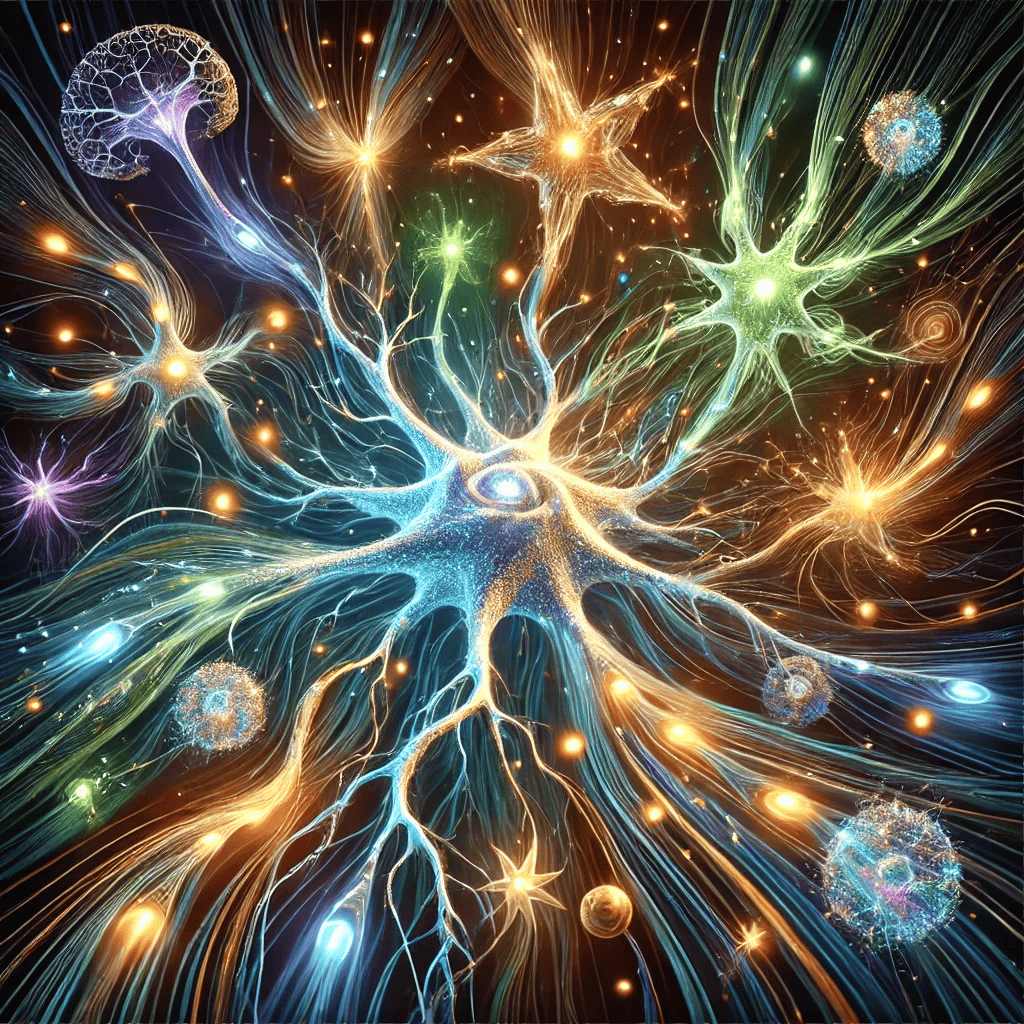
\includegraphics[width=0.8\textwidth]{light_cones.png}

    \caption{Neural light cones as a shorthand for boundary conditions of consciousness}
\end{figure}

The neural light cone concept extends beyond simple spatial and temporal boundaries to encompass the organization of energetic coherence itself. Within each cone, multiple scales of organization—from molecular interactions to regional activation patterns—must maintain alignment to support conscious processing \cite{vazquez2019gradients}. This multi-scale coherence is achieved through triangulation, where different regions within the cone maintain stable relationships through continuous mutual feedback and adjustment.

A key feature of neural light cones is their role in maintaining synchronic and diachronic unity—the integration of conscious experience across space and time respectively. Synchronic unity emerges from the capacity of regions within the cone to achieve simultaneous coherence, while diachronic unity depends on the stable propagation of coherent states across successive temporal windows \cite{tegmark2016improved}. This dual unity is maintained through the continuous operation of feedback loops that stabilize energy flows while allowing for adaptive changes in response to new inputs.

The boundaries of neural light cones are partially determined by thermal noise thresholds, which act as natural limits on the maintenance of coherent energy states \cite{oyama2009noise}. Regions within the cone must maintain sufficient energetic coherence to overcome these thermal fluctuations, while areas that cannot sustain such coherence effectively fall outside the conscious field. This creates a natural selection mechanism for conscious participation, where only those regions capable of maintaining appropriate energetic stability contribute to conscious experience.

Importantly, neural light cones are not isolated structures but form overlapping fields of influence across the cortical sheet. This overlap allows for smooth transitions in conscious experience, as different regions enter and exit the conscious field based on attention, task demands, and metabolic conditions \cite{petermann2009spontaneous}. The interaction between overlapping light cones basically creates a global light cone—a broader field of conscious integration that nonetheless remains bounded by the physical constraints on neural coherence.

The implications of the neural light cone framework extend beyond explaining current conscious experience to inform our understanding of fundamental limitations in consciousness. For instance, the model provides clear reasons why consciousness cannot be "uploaded" or transmitted across arbitrary distances—such processes would necessarily break the continuous, causally-connected energy flows that the light cone maintains \cite{seth2015granger}. Similarly, it explains why consciousness differs fundamentally from sleep states, where energy coherence patterns are altered but not destroyed, versus death, where the capacity for coherent energy maintenance is irreversibly lost.

The neural light cone also helps resolve long-standing questions about the relationship between conscious and unconscious processing. Rather than positing a rigid boundary between conscious and unconscious states, the model suggests a dynamic interface where regions move in and out of conscious awareness based on their ability to maintain coherent energy states within the light cone's boundaries \cite{tononi1998consciousness}. This fluid boundary allows for the brain's remarkable ability to shift attention and integrate new information while maintaining a stable conscious field.

Perhaps most significantly, the neural light cone framework bridges local and global aspects of conscious experience. By describing how local coherence patterns can align and integrate within broader fields of conscious awareness, it provides a physical basis for both the unity and diversity of conscious experience \cite{ramachandran2001synaesthesia}. This integration occurs through mechanisms of mutual recursion and continuous feedback, allowing for coherent diversity—the capacity to maintain distinct local patterns while contributing to a unified global experience.

The implications extend to understanding phenomena such as synaesthesia and other altered states of consciousness, where unusual patterns of integration within the neural light cone may lead to non-typical conscious experiences \cite{abraham1996metaplasticity}. The framework suggests that such phenomena emerge from modifications to the normal boundaries and integration patterns of neural light cones, rather than from purely computational or representational changes.

Understanding how neural light cones enable both local processing and global integration leads naturally to consideration of the temporal dimensions of consciousness—specifically, how the brain maintains both moment-to-moment awareness (synchronic unity) and continuous experience across time (diachronic unity) \cite{hoel2017when}. This theoretical foundation provides a bridge between the physical mechanisms of neural processing and the phenomenological features of conscious experience, suggesting new approaches to investigating both normal and altered states of consciousness.

\section{Synchronic and Diachronic Unity}

The unity of conscious experience represents one of the most compelling yet challenging aspects of consciousness to explain mechanistically. ECC approaches this challenge by distinguishing between two fundamental forms of unity—synchronic and diachronic—while showing how both emerge from underlying principles of energetic coherence within the brain's neural architecture \cite{engel2001temporal}.

Synchronic unity refers to the moment-to-moment integration of diverse conscious contents into a single, unified field of experience. Within ECC's framework, this unity is achieved not through a central processor or global workspace, but through the aligned dynamics of multiple brain regions maintaining coherent energy states \cite{singer1999neuronal}. This alignment occurs through mutual recursion, where regions continuously update their states in response to each other while maintaining stable energy patterns. Crucially, this synchronic unity operates within the constraints of the neural light cone, meaning that only regions capable of maintaining appropriate energetic coherence can participate in the unified conscious field at any given moment \cite{gray1999temporal}.

Diachronic unity describes the continuous thread of consciousness that persists across time, creating our sense of an unbroken stream of experience. ECC proposes that this temporal continuity emerges from the brain's ability to maintain stable energy configurations while smoothly transitioning between states \cite{honey2012slow}. This process relies on what might be called coherence inheritance, where each moment's conscious state builds upon and incorporates aspects of previous states while integrating new information.

The interaction between these two forms of unity is mediated by several key mechanisms. First, the brain's astrocytic networks provide a slower, more stable background against which faster neural dynamics can play out, helping to maintain continuity across moments while allowing for rapid updates to conscious content. Second, the rich alphabet of possible conscious states—defined by region-specific transcriptomic profiles—enables smooth transitions between different conscious configurations while maintaining overall coherence \cite{womelsdorf2007modulation}.

This fundamental distinction between synchronic and diachronic unity helps resolve longstanding questions about how consciousness maintains both its moment-to-moment integration and its temporal continuity \cite{vanrullen2003perception}. Understanding how these different aspects of unity emerge from patterns of energetic coherence provides new insight into both the stability and flexibility of conscious experience, while suggesting specific mechanisms through which this unity might be disrupted in various pathological conditions \cite{fell2011role}.

The maintenance of both forms of unity depends critically on coherence gradients across the cortical sheet. These gradients represent structured transitions in energy states that allow different brain regions to maintain local specificity while participating in global integration \cite{adhikari2010cross}. Unlike simpler models that posit binary transitions between conscious and unconscious processing, ECC suggests that consciousness involves continuous gradients of coherence that enable smooth transitions both spatially (across regions) and temporally (between moments).

A key insight of ECC is that synchronic and diachronic unity are not simply parallel processes but are fundamentally interlinked through shared mechanisms of energy organization \cite{wang2010neurophysiological}. The same principles that enable moment-to-moment integration of conscious contents also facilitate the smooth transition between conscious states over time. This dual role is particularly evident in the brain's handling of temporal boundaries within consciousness—the way it bridges the gap between discrete neural events and our experience of continuous, flowing consciousness \cite{vanrullen2003perception}.

However, ECC suggests that the apparent global unity of consciousness may itself be partially illusory—what we might call the framerate illusion \cite{panzeri2010sensory, harris2019conscious}. While local regions maintain genuine coherence through direct energetic coupling, the sense of complete global unity likely represents a useful fiction generated by our cognitive architecture. Much as film creates the illusion of continuous motion through discrete frames, consciousness may achieve its apparent seamlessness through sophisticated management of coherent states rather than genuine moment-to-moment continuity across the entire brain \cite{crick1990towards}.

This perspective on the partial illusoriness of global unity leads naturally to consideration of the classical binding problem \cite{roskies1999binding}. How does the brain combine different features and qualities into coherent percepts while maintaining both differentiation and integration? The binding problem represents one of the most persistent challenges in cognitive neuroscience \cite{treisman1996binding}, and ECC offers novel insights through its framework of energetic coherence and neural light cones.

\subsection{The (neural) binding problem}

The neural binding problem—how the brain integrates distributed information into unified conscious experiences—takes on new significance within Energetically Coherent Computation (ECC). While traditional accounts focus on synchronized neural firing or information integration, ECC reframes binding through the lens of energetic coherence and continuous dynamics across the cortical sheet \cite{hardcastle1999binding}.

In ECC, binding emerges from the physical organization of energy flows rather than computational synchronization alone. The framework suggests that consciousness achieves both synchronic unity (coherent experience at a moment) and diachronic unity (continuity across time) through stable, low-entropy energy fields that span relevant brain regions. These fields allow distributed information to cohere naturally through their physical dynamics, rather than requiring an explicit binding mechanism \cite{vondermalsburg1999binding}.

The key insight ECC offers regarding binding is that conscious unity does not require all information to be bound simultaneously across the entire brain. Instead, binding occurs within the constraints of the neural light cone—the region of causal connectivity that can influence conscious experience at a given moment. Information becomes bound when it achieves sufficient energetic coherence within this light cone, allowing it to contribute to the unified conscious field \cite{singer1999neuronal}.

This binding process is supported by several mechanisms in ECC. First, the rich alphabet encoded by region-specific transcriptomic profiles allows different areas to maintain distinct but compatible energy states \cite{kumar2010spiking}. Second, continuous triangulation between regions enables smooth integration of information across space and time. Third, mutual recursion and nested feedback loops help stabilize bound states while allowing for dynamic updating as new information arrives \cite{buzsaki2004neuronal}.

The brain's astrocytic networks play a crucial role in this binding process by providing a substrate for coherent energy distribution. Unlike neurons, which operate through discrete action potentials, astrocytes form syncytia—networks of cells connected by gap junctions that allow for continuous energy flows and ion redistribution. These networks help maintain the stable, low-entropy conditions necessary for conscious binding while also supporting the dynamic flexibility required for changing conscious states \cite{womelsdorf2007modulation}.

ECC thus suggests that the binding problem may be partially dissolved by recognizing consciousness as an emergent property of coherent energy fields rather than a computational challenge of synchronizing discrete signals. The framework implies that binding is not achieved through a central mechanism but arises naturally from the brain's capacity to maintain energetically coherent states across spatially distributed regions \cite{lisman2013theta}.

This perspective aligns with empirical observations about the limitations of conscious binding. Not all information can be bound simultaneously, and binding breaks down under certain conditions—precisely what we would expect if binding depends on maintaining coherent energy states within physical and thermodynamic constraints \cite{zeki1999toward}. ECC therefore offers a physically grounded account of how the brain achieves the remarkable feat of creating unified conscious experiences from distributed neural activity.

Building on this foundation, ECC's approach to the binding problem also illuminates why certain features of conscious experience emerge as they do. For instance, the limited bandwidth of consciousness—our inability to simultaneously bind unlimited information into awareness—follows naturally from the thermodynamic constraints on maintaining coherent energy fields \cite{gray1999temporal}. The brain can only sustain low-entropy coherence across a finite region at any moment, creating an inherent bottleneck in conscious processing.

The framework also explains the hierarchical nature of binding, where some features bind more readily than others. Primary sensory qualities like color and motion may bind easily because they achieve coherence within localized regions that have evolved specifically to maintain stable energy states for these features. More complex bindings, such as cross-modal associations or abstract concepts, require coherence across distributed networks and thus face greater thermodynamic challenges \cite{engel2001temporal}.

ECC's treatment of binding through energetic coherence also addresses the temporal aspects of conscious unity. The diachronic unity of consciousness—our sense of a continuous stream of experience—emerges from the brain's ability to maintain stable energy gradients across time while continuously updating their content \cite{fell2011role}. This creates a form of temporal binding that naturally bridges discrete neural events into smooth conscious transitions, explaining why we experience continuous change rather than discrete state shifts.

A particularly powerful aspect of ECC's approach is its ability to explain binding failures and alterations of consciousness. When energetic coherence is disrupted—whether through pathology, drugs, or extreme conditions—we see corresponding disruptions in conscious binding \cite{wang2010neurophysiological}. This ranges from subtle binding errors in everyday experience to profound dissociations in clinical conditions, all of which can be understood as disruptions to the brain's capacity to maintain coherent energy fields.

This reconceptualization of binding through ECC offers a bridge between phenomenology and physics, suggesting that the unity of consciousness is neither purely subjective nor simply computational, but emerges from fundamental physical principles operating under specific biological constraints. This provides a framework for understanding conscious unity that is both scientifically tractable and philosophically illuminating \cite{roskies1999binding}.

The binding problem, viewed through ECC's lens, thus becomes less about synchronizing discrete information and more about maintaining appropriate conditions for coherent energy fields. This shift in perspective suggests new directions for research, focusing on how biological systems achieve and maintain the specific forms of energetic coherence necessary for conscious experience \cite{kumar2010spiking}. It also raises intriguing questions about the minimum physical requirements for conscious binding, potentially informing both our understanding of consciousness in simpler organisms and the development of artificial conscious systems \cite{buzsaki2004neuronal}.

This theoretical framework naturally leads us to consider the fundamental mechanisms through which neural systems encode and process information. Two distinct but complementary coding schemes emerge as particularly relevant: rate coding, which conveys information through average firing frequencies, and temporal coding, which utilizes precise spike timing relationships. Understanding how these coding strategies contribute to energetic coherence provides crucial insight into how the brain maintains both stable representations and dynamic flexibility in conscious processing \cite{panzeri2010sensory, lisman2013theta}. The interplay between these coding mechanisms illuminates how neural systems achieve the sophisticated information processing necessary for conscious experience while maintaining coherent energy states.

\subsection{Rate vs Temporal Coding}

Rate and temporal coding represent two fundamental mechanisms through which neural systems process information, each offering distinct advantages while likely operating in complementary ways. Rate coding, which conveys information through the average firing frequency of neurons over time, provides robustness against noise and supports stable representations across longer timescales \cite{kumar2010spiking}. This aligns with ECC's emphasis on maintaining coherent energy states, as rate-based coding allows for reliable signal transmission while managing thermal fluctuations and other sources of noise.

Temporal coding, in contrast, utilizes the precise timing of action potentials to encode information, enabling higher information capacity and rapid processing \cite{panzeri2010sensory}. Within ECC's framework, temporal coding can be understood as supporting fine-grained patterns of energetic coherence, particularly in systems requiring precise synchronization or phase relationships. Recent work has demonstrated that spike timing measures reveal stronger attentional effects and provide more robust stimulus representations that are modulated by task demands \cite{zhang2023adaptive}.

The complementarity of these coding schemes becomes particularly evident in sensory processing \cite{buzsaki2004neuronal}. Early sensory systems often employ rate coding to represent stimulus intensity, where the steady-state energy flow captured by firing rates provides reliable encoding of persistent features. Higher-order processing may shift toward temporal coding, especially in cases requiring precise timing relationships, such as sound localization or motion detection \cite{womelsdorf2007modulation}. This transition from rate to temporal coding parallels ECC's description of how information becomes integrated into increasingly sophisticated patterns of energetic coherence.

Notably, the brain appears to shift dynamically between these coding strategies depending on computational demands and energy constraints \cite{lisman2013theta}. Rate coding predominates in situations requiring stable, long-term representations or resistance to noise, while temporal coding emerges in contexts demanding precise temporal integration or rapid state transitions. This flexibility aligns with ECC's emphasis on how conscious systems maintain coherent states while adapting to changing conditions.

This understanding suggests that rather than viewing rate and temporal coding as competing theories, they represent different manifestations of how biological systems achieve energetic coherence under varying constraints \cite{fell2011role}. The brain's ability to seamlessly integrate both coding schemes reflects its sophisticated capacity for managing energy dynamics across multiple temporal and spatial scales, a key feature highlighted by the ECC framework.

Through ECC's lens, rate and temporal coding represent different mechanisms by which neural systems achieve and maintain energetic coherence. Rate coding manifests as stable patterns of energy flow, where consistent firing frequencies create sustained fields of coherent activity. These patterns align with ECC's emphasis on low-entropy states that can reliably maintain conscious processing while managing thermal noise and other perturbations \cite{wang2010neurophysiological}.

Temporal coding, by contrast, enables more sophisticated patterns of energetic coherence through precise spike timing. Within ECC's framework, temporal coding supports the creation of complex interference patterns in the neural tissue's energetic fields \cite{adhikari2010cross}. These patterns, shaped by the precise timing of action potentials relative to ongoing oscillations, create rich spatiotemporal structures that support higher-order conscious processing \cite{buzsaki2004neuronal}.

The astrocytic networks emphasized by ECC play a crucial role in regulating the balance between rate and temporal coding. Through their slower calcium dynamics and gap junction coupling, astrocytes help maintain stable background states that support rate coding while simultaneously modulating the conditions necessary for precise temporal coding in neuronal populations \cite{honey2012slow}. This dual regulation exemplifies how biological systems achieve the sophisticated energy management required for conscious processing.

The relationship between local and global aspects of consciousness also becomes clearer through this framework \cite{singer1999neuronal}. While traditional theories often struggle to explain how localized neural activity contributes to unified conscious experience, ECC's coherence-based approach shows how local patterns of energetic coherence can integrate into global conscious states through principled physical mechanisms. This integration is not merely additive but involves the maintenance of coherent energy dynamics across multiple scales.

Recent experimental evidence supports this integrated view of neural coding. Studies have shown that attention and task demands can flexibly modulate the relative contribution of rate and temporal codes, with temporal coding showing particular sensitivity to cognitive demands and providing more detailed stimulus representations \cite{zhang2023adaptive}. This adaptability in coding strategies reflects the brain's capacity to optimize its energy coherence patterns based on current processing requirements.

The relationship between rate and temporal coding thus reveals fundamental principles about how neural systems achieve and maintain the coherent energy states necessary for conscious processing. Rather than representing competing frameworks, these coding schemes reflect complementary mechanisms through which the brain establishes patterns of energetic coherence across multiple spatial and temporal scales \cite{lisman2013theta}. Understanding these mechanisms requires moving beyond traditional computational approaches to consider how biological systems achieve and maintain coherent states through their rich molecular and cellular architecture.

This leads us to consider a crucial aspect of how neural systems maintain coherent conscious states: the diverse repertoire of possible states shaped by transcriptomic profiles and molecular diversity \cite{zhang2023adaptive}. These rich alphabets of potential configurations provide the foundation for both the stability and flexibility of conscious experience, enabling sophisticated information processing while maintaining energetic coherence. Understanding how these molecular mechanisms support conscious unity represents a crucial next step in developing a comprehensive theory of consciousness.

\section{Rich Alphabets and Transcriptomic Profiles}

The brain's ability to maintain both unified and differentiated conscious states depends critically on what ECC terms "rich alphabets"—diverse repertoires of possible states that are physically grounded in the unique molecular characteristics of different neural populations. These alphabets are not arbitrary but are shaped by specific transcriptomic profiles that determine how different brain regions can participate in conscious processing \cite{tasic2018shared, siletti2023transcriptomic}.

The concept of rich alphabets in ECC represents a fundamental departure from traditional computational approaches to consciousness. Rather than viewing neural information processing as manipulation of abstract symbols, ECC proposes that conscious states emerge from physically grounded alphabets of possible energy configurations, each shaped by the unique molecular and genetic characteristics of different neural populations \cite{bakken2021comparative}. These alphabets are not merely metaphorical but are directly instantiated in the specific transcriptomic profiles that define how different brain regions process and integrate information \cite{hawrylycz2016inferring}.

At its core, the rich alphabet concept suggests that consciousness requires more than binary or discrete states; it demands a continuous, multi-dimensional space of possible configurations that can support the nuanced variations of conscious experience \cite{cembrowski2018continuous}. This richness emerges from the complex interplay between gene expression patterns, protein states, and energetic dynamics within neural tissues. The transcriptomic profiles of different brain regions effectively define the vocabulary available for conscious processing in each area, determining both the range and precision of possible conscious states \cite{lake2016neuronal}.

The framework identifies several key features that characterize these rich alphabets. First, they exhibit nested diversity—hierarchical organizations of possible states that allow for both broad categorization and fine-grained discrimination \cite{nowakowski2017spatiotemporal}. Second, they maintain adaptive stability—the capacity to sustain specific conscious states while allowing for smooth transitions between them \cite{raj2008nature}. Third, they demonstrate context-sensitive modulation—the ability to adjust their repertoire of available states based on current conditions and requirements \cite{lein2017promise}.

These features are directly grounded in the transcriptomic profiles of neural populations, which determine the specific proteins, receptors, and signaling molecules available in different brain regions \cite{saunders2018molecular}. This molecular foundation provides the physical basis for the rich alphabets that support conscious processing, creating energetic vocabularies unique to each brain area \cite{yuste2020community}. Recent advances in single-cell RNA sequencing have revealed unprecedented detail about the molecular diversity of neural populations, providing empirical support for the concept of rich alphabets in neural processing \cite{macosko2015highly, zeisel2015cell}.

Within the framework of rich alphabets and transcriptomic profiles, ECC offers a novel perspective on how to conceptualize and study similarity between brain states. Unlike traditional approaches that rely on abstract representational spaces or purely functional similarities, ECC grounds neural similarity in the physical instantiation of states within the brain's energetic and molecular landscape (cf. \cite{bobadilla-suarez2020measures}).

The framework suggests that similarity between neural states emerges naturally from the physical constraints imposed by transcriptomic profiles and their associated rich alphabets \cite{thompson2014human}. Rather than requiring an arbitrary choice of similarity metric—a persistent challenge in both cognitive science and machine learning—ECC proposes that similarity is inherently defined by the physical properties of the underlying neural substrate \cite{trapnell2015defining}. This grounding provides a principled basis for understanding how different conscious states relate to one another.

Just as modern machine learning systems create embedding spaces where similar concepts cluster together, the brain's rich alphabets combine to create physically grounded embedding spaces. However, unlike artificial embedding spaces, which often lack clear physical interpretation, these neural embedding spaces are directly constrained by the molecular and energetic properties of brain tissue \cite{wang2018three}. The dimensions of these spaces are not arbitrary but reflect the actual degrees of freedom available within the brain's transcriptomic landscape \cite{tasic2018shared}.

This perspective offers several key insights for studying neural similarity. First, it suggests that similarity metrics should be derived from the physical properties of neural systems rather than imposed externally \cite{bakken2021comparative}. Second, it predicts that similar conscious states should exhibit similar patterns of energetic coherence, reflecting their proximity in the physically grounded embedding space. Third, it implies that the brain's capacity for differentiated conscious states is fundamentally limited by the richness of its molecular alphabet \cite{cembrowski2018continuous}.

The physically grounded embedding spaces created by rich alphabets not only provide a framework for understanding neural similarity but also help explain how the brain achieves both differentiation and integration in conscious experience. These spaces are not static but dynamically adapt through contextual modulation—shifts in the available repertoire of states based on current cognitive demands and physiological conditions \cite{lein2017promise}.

This dynamic nature of rich alphabets reveals a crucial principle: the brain's representational capacity is not fixed but exists within thermodynamic constraints that shape which configurations are available at any given time \cite{hawrylycz2016inferring}. The transcriptomic profiles that define these alphabets must balance expressive power against metabolic efficiency, creating energetically optimized vocabularies for conscious processing \cite{lake2016neuronal}.

Understanding rich alphabets and their physical grounding ultimately provides insight into why consciousness cannot be reduced to purely computational processes. The specific molecular and energetic properties that create these alphabets cannot be abstracted away from their physical implementation—they are essential to how consciousness emerges and maintains coherence \cite{siletti2023transcriptomic}. Recent advances in spatial transcriptomics have revealed increasingly sophisticated patterns of molecular organization across brain regions, supporting the idea that conscious processing requires specific patterns of gene expression and protein states \cite{macosko2015highly}.

The implications extend beyond theoretical understanding to practical applications in neuroscience and medicine. By recognizing how transcriptomic profiles shape conscious processing, we gain new insights into both normal brain function and pathological conditions \cite{nowakowski2017spatiotemporal}. This biological grounding suggests new approaches to treating disorders of consciousness by targeting the molecular mechanisms that support coherent conscious states \cite{yuste2020community}.

These theoretical insights about rich alphabets and their role in conscious processing lead naturally to consideration of how these molecular mechanisms interact with thermal noise and other physical constraints \cite{raj2008nature}. Understanding the relationship between transcriptomic diversity and thermodynamic boundaries helps explain both the possibilities and limitations of conscious processing, providing a bridge between molecular mechanisms and physical constraints \cite{zeisel2015cell}.

This transition from molecular mechanisms to physical constraints highlights how the richness of conscious experience, enabled by transcriptomic diversity, must nonetheless operate within physical constraints—chief among them the omnipresent influence of thermal noise in biological systems \cite{trapnell2015defining}. The next section examines how these physical constraints shape and bound conscious processing while contributing to its remarkable stability and flexibility.

\section{Thermal Noise as Boundary Conditions}

Among the physical constraints that shape conscious processing, thermal noise plays a particularly crucial role. Rather than representing mere background interference, thermal fluctuations establish fundamental boundaries on how the brain can maintain coherent conscious states. These boundaries are not arbitrary limitations but emerge directly from the thermodynamic properties of neural tissue \cite{faisal2008}.

ECC suggests that thermal noise serves a dual function in conscious processing—acting both as a constraint that bounds possible states and as a resource that contributes to system stability. Unlike digital computers that must suppress noise to maintain reliable operation \cite{vanderziel1988}, biological systems have evolved to function effectively within, and even exploit, thermal fluctuations. This perspective aligns with recent theoretical work suggesting that noise plays a constructive role in neural information processing \cite{mcdonnell2011}.

The framework draws particular attention to how thermal noise influences different aspects of neural function. At the molecular level, thermal fluctuations affect ion channel dynamics and neurotransmitter release \cite{attwell2001}. At cellular scales, they influence membrane potentials and action potential generation. At network levels, they contribute to the variability in neural firing patterns and synchronization \cite{schreiber2003}. Rather than treating these effects as mere impediments, ECC suggests they help establish the natural boundaries within which conscious processing must operate.

This perspective aligns with emerging understanding of how biological systems manage energy and information. Recent work has demonstrated that neural systems operate remarkably close to fundamental thermodynamic limits \cite{laughlin2001}, suggesting that the brain has evolved sophisticated mechanisms for maintaining coherent states despite omnipresent thermal fluctuations. These mechanisms don't simply suppress noise but rather incorporate it into their functional architecture \cite{harris2012}.

The relationship between thermal noise and conscious processing reveals itself through several key phenomena. Stochastic resonance, where moderate levels of noise actually enhance signal detection, demonstrates how neural systems can leverage thermal fluctuations constructively \cite{gammaitoni1998}. Similarly, the role of noise in enabling state transitions suggests it contributes to the brain's capacity for flexible, adaptive response \cite{mcdonnell2009}.

In ECC, thermal noise manifests through multiple channels or "flavors" that collectively establish the boundaries within which conscious processing must operate. These different forms of noise—mechanical, chemical, and electrical—each contribute distinct constraints to the brain's capacity for maintaining coherent conscious states \cite{faisal2008}. Understanding how these various forms of noise interact and influence neural dynamics is crucial for grasping the physical limitations on consciousness.

Mechanical noise emerges from the physical movement of cellular components and structures within the brain. This includes membrane fluctuations, cytoskeletal vibrations, and the dynamic reorganization of proteins and other macromolecules \cite{bialek2012}. Such mechanical fluctuations create a baseline of physical perturbation that any coherent conscious state must overcome. The framework suggests that biological systems have evolved specific mechanisms to manage these fluctuations while maintaining functional coherence \cite{niven2008}.

Chemical noise arises from the stochastic nature of molecular interactions within neural tissue. This encompasses fluctuations in neurotransmitter release, random variations in receptor-ligand binding, and the inherent variability in cellular signaling cascades \cite{attwell2001}. These chemical fluctuations are particularly relevant to how rich alphabets, defined by transcriptomic profiles, can maintain stable states despite constant molecular turnover. The brain manages chemical noise through molecular redundancy—multiple parallel pathways that help ensure reliable signaling despite local fluctuations \cite{harris2012}.

Electrical noise manifests in the form of random fluctuations in membrane potentials, ion channel dynamics, and local field potentials \cite{vanderziel1988}. This electrical component of thermal noise directly influences the brain's ability to maintain coherent energy states across neural populations. However, rather than simply representing a limitation, electrical noise can sometimes contribute to signal detection through phenomena like stochastic resonance, where moderate levels of noise actually enhance the detection of weak signals \cite{gammaitoni1998}.

The interaction between these different flavors of noise—mechanical, chemical, and electrical—creates noise landscapes across the brain. These landscapes are not uniform but vary according to local tissue properties, metabolic states, and transcriptomic profiles \cite{laughlin2001}. Understanding how these noise landscapes shape conscious processing helps explain both the limitations and adaptive features of consciousness.

Critically, ECC suggests that the brain does not merely cope with these various forms of noise but has evolved to exploit them in specific ways \cite{mcdonnell2011}. For instance, moderate levels of noise can enhance the stability of conscious states through stochastic stabilization—where random fluctuations actually help maintain broader patterns of coherence. This represents a fundamental difference from artificial computing systems, which typically treat noise as purely detrimental \cite{keizer1987}.

Recent theoretical work suggests that noise may play an essential role in neural computation and consciousness, contributing to phenomena such as state transitions and decision-making \cite{rolls2010}. The framework proposes that conscious processing operates within an optimal noise regime—neither too chaotic to maintain coherent states nor too rigid to allow adaptive responses. This balance reflects fundamental principles about how biological systems manage information and energy \cite{sejnowski2014}.

The implications of this perspective extend beyond theoretical understanding to practical applications in medicine and artificial intelligence. Understanding how biological systems maintain conscious states in the presence of thermal noise suggests new approaches to treating disorders of consciousness and designing artificial systems that could potentially support conscious-like processing \cite{parrondo2015}. Rather than attempting to eliminate noise entirely, such approaches might focus on achieving appropriate balance between stability and flexibility.

Furthermore, the framework suggests that thermal noise plays a crucial role in establishing the boundaries of conscious experience \cite{fox2007}. These boundaries are not fixed but emerge dynamically from the interaction between energetic coherence and thermal fluctuations. This helps explain why consciousness exhibits both stability and flexibility—it operates within thermal constraints that simultaneously limit and enable adaptive processing.

This theoretical framework naturally leads to consideration of the fundamental nature of energy in conscious systems \cite{attwell2001}. Understanding how thermal noise constrains and shapes conscious processing requires careful examination of how energy manifests and flows within neural tissues. The next section explores the physical foundations of energy in conscious systems, examining both its practical manifestations and deeper theoretical implications.

\section{Energy and Its Physical Foundations}

The nature of energy in conscious systems represents a foundational challenge for any theory attempting to bridge physical and experiential aspects of consciousness. As noted in seminal work on physical chemistry \cite{Atkins2010}, energy manifests in multiple forms and undergoes complex transformations, yet maintains fundamental conservation principles that constrain all physical processes. In conscious systems, these energy dynamics take on particular significance, operating at multiple scales from molecular interactions to global brain states, while maintaining the coherent patterns necessary for conscious experience \cite{Demetrius2015}.

Understanding energy in consciousness requires moving beyond simple mechanical or thermodynamic descriptions to consider how biological systems achieve and maintain specific patterns of energetic coherence. As emphasized in theoretical work on biological energy systems \cite{Qian2007}, living organisms employ sophisticated mechanisms for managing energy flows and maintaining low-entropy states crucial for information processing. This perspective aligns with fundamental insights about the relationship between energy, symmetry, and physical law articulated in Noether's theorem \cite{Kosmann-Schwarzbach2011}, suggesting that consciousness may emerge from specific patterns of energy organization that preserve certain symmetries while enabling controlled symmetry breaking for adaptive response.

\subsection{Energy as Useful Work}

Traditional physics defines energy through its capacity to perform useful work—a deceptively simple concept that becomes more complex when applied to biological systems. In mechanical and thermodynamic contexts, useful work represents directed, organized change: the movement of a piston, the flow of electrical current, or the synthesis of molecules \cite{Atkins2010}. Heat dissipation typically represents the waste output of such processes, energy that disperses into the environment rather than contributing to organized work.

However, ECC suggests that this traditional dichotomy between useful work and heat dissipation requires refinement when considering conscious systems. In the brain, what constitutes useful work extends beyond simple mechanical or chemical transformations \cite{Qian2007}. The maintenance of coherent conscious states involves continuous energy expenditure that might appear wasteful from a purely mechanical perspective but serves essential functions in sustaining consciousness. This includes maintaining membrane potentials, supporting synchronized oscillations, and enabling the dynamic reorganization of neural networks.

Moreover, what traditionally might be classified as dissipative processes often play crucial functional roles in conscious systems \cite{Nicolis1977}. The brain's ability to maintain low-entropy, coherent states paradoxically depends on controlled energy dissipation through what \cite{Prigogine1978} terms structured dissipation. Unlike simple heat loss, this structured dissipation helps maintain the dynamic stability necessary for conscious processing. The framework suggests that consciousness requires a delicate balance between energy conservation and controlled dissipation, creating what might be termed dissipative coherence.

This perspective challenges us to reconsider how we define energy in the context of consciousness \cite{Demetrius2015}. Rather than focusing solely on mechanical work or heat dissipation, ECC proposes that energy in conscious systems must be understood through its role in maintaining coherent, information-rich states across multiple scales of organization. This aligns with recent theoretical work suggesting that biological systems achieve remarkable efficiency in energy utilization while maintaining the complex dynamics necessary for consciousness \cite{Laughlin2005}.

\subsection{Types of Energy}

The major forms of energy recognized in physics find direct analogues in neural systems, though their manifestations and interactions in the brain exhibit unique properties relevant to consciousness \cite{Atkins2010}. Understanding these parallels helps illuminate how the brain integrates different forms of energy to maintain conscious states.

Mechanical energy in neural systems manifests through multiple mechanisms. Potential energy exists in the physical structure and tension of cellular components, particularly in the cytoskeleton and membrane conformations. Kinetic energy appears in the movement of cellular structures, vesicle transport, and fluid dynamics of the cerebrospinal fluid \cite{Shulman2013}. Mechanical waves propagate through neural tissue, potentially contributing to information integration and energy distribution, while pressure gradients and mechanical forces influence cell signaling and neural activity.

Chemical energy plays a central role in neural function, with ATP serving as the primary carrier of chemical energy, driving countless cellular processes \cite{Qian2007}. Concentration gradients of ions across membranes store potential energy that can be rapidly converted to electrical signals. The processes of neurotransmitter synthesis, release, and recycling represent crucial chemical energy transformations, while metabolic processes create and maintain the energy availability necessary for sustained conscious processing \cite{Demetrius2015}.

Electrical energy in neural systems takes several forms. Membrane potentials store electrical energy in the form of ion gradients, while action potentials represent rapid electrical energy transformations \cite{Street2016}. Local field potentials and brain waves reflect larger-scale electrical phenomena, and electromagnetic fields emerge from coordinated electrical activity. These different forms of energy interact in complex ways that ECC suggests are essential for consciousness. For instance, chemical energy from ATP drives ion pumps that maintain electrical gradients, electrical signals trigger mechanical changes in synaptic structures, and mechanical forces can influence ion channel function and thus electrical signaling \cite{Laughlin2005}.

The mathematical formalism needed to describe these various forms of energy and their interactions can be developed within ECC using the Jacobian of the stress-energy tensor, where each energy type represents a distinct subsystem with its own dynamics and coupling terms \cite{Coopersmith2017}. This mathematical framework allows us to track how different forms of energy flow, transform, and maintain coherent states across the brain. The tensor approach is particularly powerful because it captures both the local energy dynamics within each subsystem and the crucial coupling terms that describe how different forms of energy interact at their interfaces.

\subsection{Energy as Noether's Time Invariant}

Emmy Noether's profound insight into the relationship between symmetries and conservation laws provides a fundamental framework for understanding energy in conscious systems \cite{Kosmann-Schwarzbach2011}. Her theorem reveals that energy conservation is not merely an empirical observation but emerges from a fundamental symmetry in physical law—specifically, the symmetry of physical laws under translations in time. This perspective suggests that energy is, at its deepest level, a manifestation of temporal invariance in physical systems \cite{Neuenschwander2017}.

For ECC, Noether's insight has crucial implications. It suggests that the brain's capacity to maintain conscious states may be intimately linked to its ability to preserve certain symmetries across time while managing controlled symmetry breaking in others \cite{Brading2002}. The framework proposes that consciousness requires a delicate balance between conserved quantities (enabling stable conscious states) and symmetry-breaking processes (allowing for dynamic transitions between states) \cite{Weyl1952}.

This understanding of energy—as both a practical capacity for doing work and a fundamental manifestation of temporal symmetry—provides the foundation for how ECC conceptualizes consciousness as an emergent property of coherent energy flows \cite{Feynman1963}. It shows why consciousness cannot be reduced to computation alone but must be understood through the lens of physical processes operating under fundamental conservation laws and symmetry principles \cite{Laughlin2005}.

The implications of Noether's theorem for consciousness extend beyond theoretical considerations to practical understanding of how biological systems maintain coherent states. The brain's ability to preserve certain symmetries while breaking others may be essential for generating the specific patterns of energetic coherence that support conscious experience \cite{Nicolis1977}. This suggests that consciousness emerges not just from energy flows per se, but from the sophisticated management of symmetries and conservation laws that these flows represent \cite{Coopersmith2017}.

Furthermore, viewing energy through Noether's theorem helps explain why consciousness requires specific types of physical organization. The maintenance of coherent conscious states may depend on the brain's ability to establish and preserve particular temporal symmetries while allowing for controlled symmetry breaking that enables adaptive response \cite{Prigogine1978}. This perspective provides a deeper theoretical foundation for understanding how consciousness emerges from physical systems while maintaining its distinctive phenomenological features.

\section{Energetic Coherence and Field Dynamics}

The implications of viewing energy through both its practical manifestations (mechanical, chemical, electrical) and its fundamental nature (as a consequence of temporal symmetry) lead us to consider how these energy flows achieve the coherent patterns necessary for consciousness. Unlike simpler physical systems where field dynamics might be dominated by a single type of interaction, conscious processing requires the integration and coordination of multiple field types—electromagnetic, chemical, and mechanical—into stable, yet adaptable patterns of activity \cite{Freeman2006}.

These fields do not exist in isolation but form coupled field dynamics, where different types of fields influence and stabilize each other through continuous feedback \cite{McFadden2002}. The electromagnetic fields generated by neural activity interact with mechanical forces in cell membranes and chemical gradients across cellular compartments, creating a rich, multi-dimensional landscape of interacting field effects that supports conscious processing \cite{Pockett2012}. Recent theoretical work has suggested that these field interactions may play a crucial role in binding information across different brain regions and timescales \cite{Nunez2010}.

The concept of field coherence in ECC extends beyond simple synchronization or correlation to encompass multi-scale resonance \cite{Singer2009}. This resonance manifests across different spatial and temporal scales, from molecular interactions to global brain states, creating stable patterns that can nonetheless adapt rapidly to changing conditions. Unlike classical field theories that might focus solely on electromagnetic or chemical gradients, ECC emphasizes how multiple field types must achieve coherence while maintaining their distinct functional roles \cite{Haken2006}.

Central to this framework is the concept of field stability through mutual constraint \cite{Barrett2014}. Each type of field—electromagnetic, chemical, and mechanical—imposes constraints on the others, creating a web of interdependencies that helps maintain overall coherence. These constraints operate across multiple scales, from molecular interactions to global brain states, nested coherence \cite{Raichle2006}. This multi-scale organization allows conscious systems to maintain both local specificity and global integration, a feature that has proven challenging to explain through traditional computational approaches.

Recent experimental evidence has begun to support this theoretical framework, demonstrating how different field types interact to create stable patterns of neural activity \cite{DelGiudice1985}. These studies suggest that consciousness may indeed emerge from the coordinated interaction of multiple field types, rather than from any single type of neural activity or computation alone \cite{Atasoy2019}. This perspective helps explain both the stability and flexibility of conscious experience, while suggesting new approaches to investigating the neural basis of consciousness.

\begin{figure}[h]
    \centering
    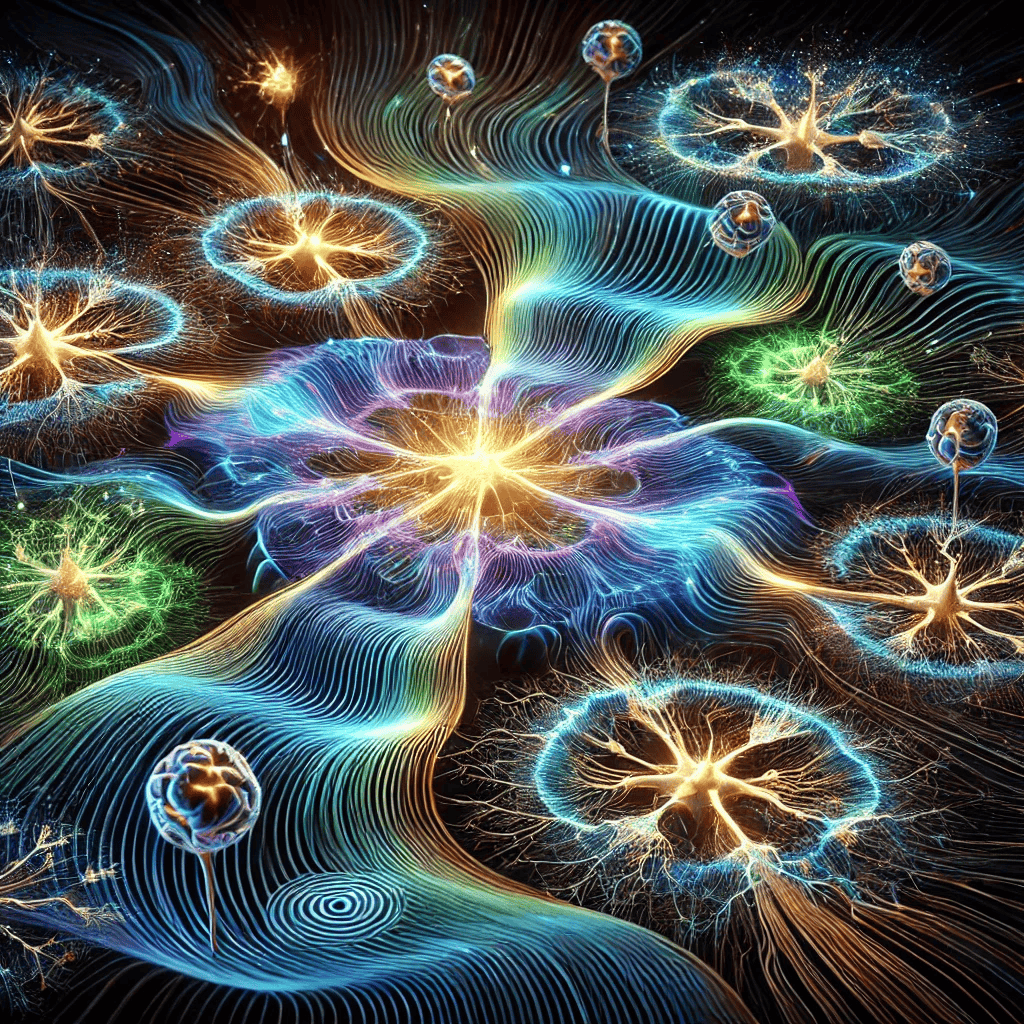
\includegraphics[width=0.8\textwidth]{fields.png}

    \caption{Electromagnetic fields bring an extra layer of integration and coherence for consciousness}
\end{figure}

The relationship between local and global field dynamics in conscious systems reveals the need for sophisticated organizing principles that maintain coherence across multiple scales \cite{Freeman2006}. Rather than relying on centralized control, consciousness appears to emerge from distributed patterns of field interaction that achieve stability through mutual constraint and continuous feedback \cite{Nunez2010}. This distributed organization allows for both the integration necessary for unified conscious experience and the differentiation required for complex information processing.

Studies of electromagnetic field dynamics in neural tissue have revealed intricate patterns of coordination that may be essential for conscious processing \cite{McFadden2002}. These fields appear to play a crucial role in binding information across different brain regions, creating field-mediated integration \cite{Pockett2012}. The interaction between electromagnetic fields and other types of fields—mechanical and chemical—creates a rich landscape of possible states that supports the complexity of conscious experience.

Recent theoretical work has suggested that these field interactions may operate near critical points, allowing for maximum flexibility while maintaining stability \cite{Haken2006}. This critical dynamics enables conscious systems to respond rapidly to changing conditions while preserving coherent patterns of activity across multiple scales. The framework proposes that consciousness requires specific types of field organization that balance stability with adaptability, (metastable dynamics) \cite{Kelso2012}.

The maintenance of field coherence in conscious systems appears to depend on sophisticated mechanisms for energy management and distribution \cite{Raichle2006}. Unlike simpler physical systems, conscious brains must maintain specific patterns of field interaction while continuously processing new information and updating their internal states. This requires dynamic stability—the ability to maintain coherent patterns while allowing for continuous modification and adaptation \cite{Singer2009}.

These field dynamics create coherence landscapes across the brain—regions of possible field configurations that support different aspects of conscious processing \cite{Atasoy2019}. These landscapes are not static but continuously evolve based on current conditions and processing demands, allowing conscious systems to maintain stability while adapting to changing circumstances. This dynamic organization helps explain both the stability and flexibility of conscious experience.

Critical to understanding these field dynamics is recognizing how different types of coherence interact and reinforce each other \cite{Freeman2006}. Chemical gradients provide boundary conditions for electromagnetic fields, while mechanical forces influence both chemical and electrical properties of neural tissue. This mutual interdependence creates cross-modal coherence \cite{DelGiudice1985}, where stability in one domain helps maintain coherence in others.

The mathematical description of these interacting fields requires sophisticated tools that can capture both their individual dynamics and their collective behavior \cite{Barrett2014}. The framework employs tensor mathematics to describe how different field types couple and interact, detailing field tensors that characterize the overall state of the system \cite{Aharonov1959}. These mathematical structures help explain how conscious systems maintain coherence across multiple scales while allowing for flexible adaptation to changing conditions.

Recent theoretical developments have suggested that consciousness may require specific patterns of field organization that cannot be reduced to simpler physical descriptions \cite{Nunez2010}. These patterns involve nested coherence hierarchies, where field interactions at different scales support and stabilize each other \cite{Wennekers2009}. This hierarchical organization helps explain how conscious systems maintain both local specificity and global integration, a feature that has proven challenging to account for through traditional computational approaches.

The framework's emphasis on field dynamics naturally leads to consideration of more formal mathematical tools for describing how local patterns of coherence combine into stable, globally coherent states \cite{Haken2006}. This transition from qualitative understanding to rigorous mathematical description represents a crucial step in developing a comprehensive theory of consciousness based on energetic coherence. The following section introduces the mathematical formalism needed to describe these complex field interactions and their role in conscious processing.

\section{Mathematical Formalism}

The complexity of field interactions in conscious systems requires a sophisticated mathematical framework capable of describing both local dynamics and global coherence. ECC employs several complementary mathematical approaches to capture these phenomena: sheaf theory provides tools for understanding how local coherence combines into global states; the Jacobian of the stress-energy tensor describes energy flows and their transformations; coupling and interface terms capture interactions between different subsystems; while triangulation and mutual recursion help explain how coherence is maintained across scales.

These mathematical tools are not merely descriptive but provide insight into how consciousness emerges from physical processes. By combining sheaf-theoretic approaches with physical tensors and dynamical principles, we can begin to formalize how the brain achieves the remarkable feat of maintaining coherent conscious states. The qualitative understanding of field dynamics naturally leads to the need for rigorous mathematical tools to describe conscious processes in physical systems.

These interconnected field dynamics, while qualitatively instructive, require precise mathematical formalization to describe how local coherence patterns combine into global conscious states. Particularly crucial is understanding how different regions maintain their specialized functions while contributing to unified conscious experience. This leads us to adopt sophisticated mathematical tools that can capture both the local structure and global integration of conscious processing.

\section{Sheaf Theory}

Sheaf theory provides a natural mathematical framework for describing how local coherent states combine into global conscious experience. Let $X$ represent the topological space of the brain's cortical sheet, with open sets $U \subseteq X$ corresponding to different cortical regions. A sheaf $\mathcal{F}$ on $X$ assigns to each open set $U$ a collection $\mathcal{F}(U)$ of local sections—mathematical objects that represent coherent energy states within that region.

\begin{figure}[h]
    \centering
    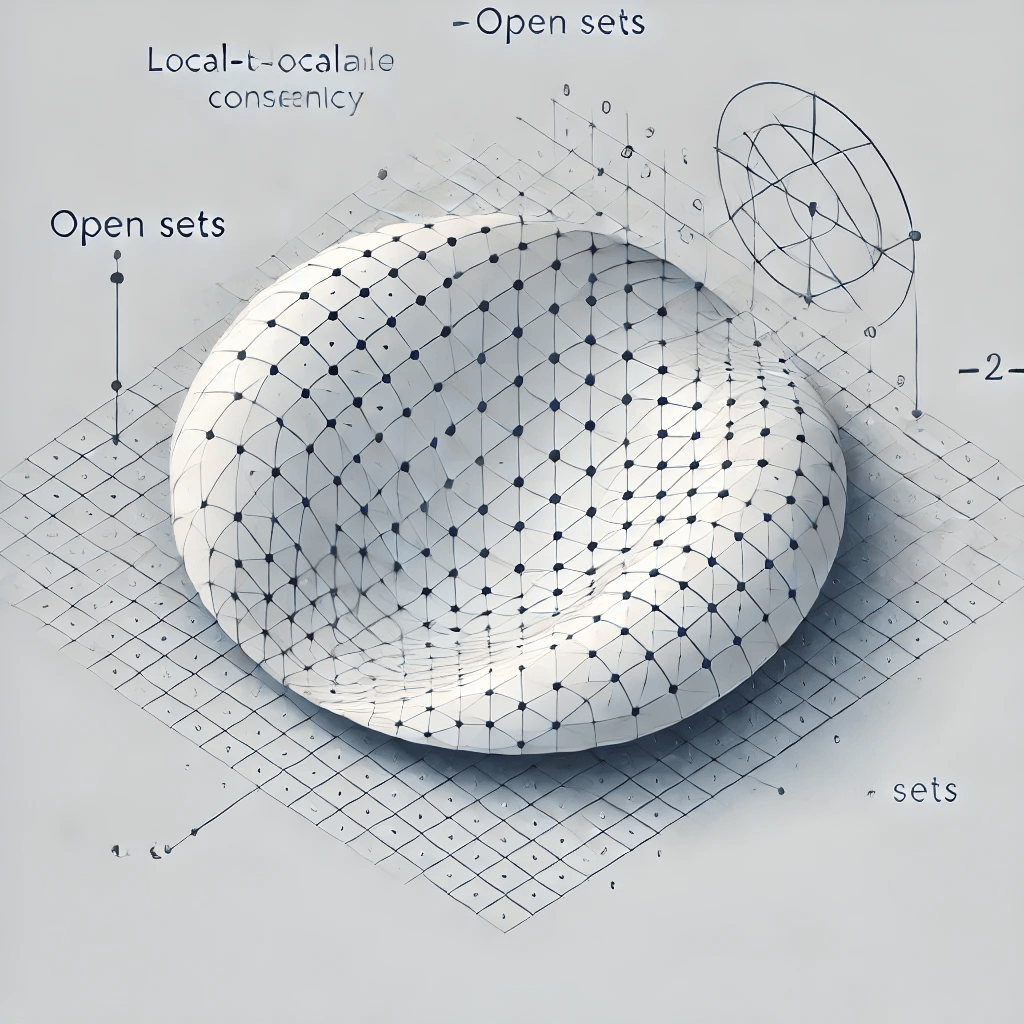
\includegraphics[width=0.8\textwidth]{sheaves.png}

    \caption{Sheaves help us define gluing conditions for consciousness (from local-to-global dynamics)}
\end{figure}

For any two overlapping regions $U$ and $V$, the sheaf includes restriction maps:

\begin{align}
\rho U \cap V: \mathcal{F}(U) \rightarrow \mathcal{F}(U \cap V)
\\
\rho V \cap U: \mathcal{F}(V) \rightarrow \mathcal{F}(U \cap V)
\end{align}


These maps must satisfy the crucial compatibility condition that for any sections $s \in \mathcal{F}(U)$ and $t \in \mathcal{F}(V)$:

$\rho U \cap V(s) = \rho V \cap U(t)$ on $U \cap V$

This compatibility ensures that local coherent states "glue" together properly across regional boundaries. The sheaf structure thus formalizes how consciousness maintains both local specialization and global integration through coherent gluing conditions. These conditions can be expressed through diagrams:

$\mathcal{F}(U) \rightarrow \mathcal{F}(U \cap V) \leftarrow \mathcal{F}(V)$

where the arrows represent restriction maps that must commute for consciousness to maintain coherence.

To capture the rich dynamics of conscious processing, we enhance the basic sheaf structure with additional mathematical machinery. Let $s \in \mathcal{F}(U)$ represent a local section corresponding to a coherent energy state in region U. The section s can be represented as a tuple:

$s = (E, \psi, \phi, \tau)$

where:

- $E$ represents the energy configuration

- $\psi$ captures the electromagnetic field state

- $\phi$ describes chemical gradients

- $\tau$ encodes the transcriptomic profile influencing local dynamics

The global behavior of consciousness emerges from coherent sheaf dynamics, where multiple local sections must satisfy compatibility conditions across overlapping regions. For regions $U$, $V$, $W$ with non-empty intersections, we require:

1. Binary Compatibility:
$\rho_{U \cap V}(s_U) = \rho_{V \cap U}(s_V) \text{ on } U \cap V$

2. Triple Overlap Condition:
$\rho_{U \cap V \cap W}(s_U) = \rho_{V \cap W \cap U}(s_V) = \rho_{W \cap U \cap V}(s_W) \text{ on } U \cap V \cap W$

These conditions ensure hierarchical coherence stability. The framework introduces a coherence measure $\mu$ that quantifies the degree of alignment between local sections:

$\mu(s_U, s_V) = \int_{U \cap V} \|\rho_{U \cap V}(s_U) - \rho_{V \cap U}(s_V)\|^2 \,d\nu$

where $d\nu$ represents an appropriate measure on the overlap region. Conscious processing requires that $\mu$ remains below certain thresholds determined by the brain's energetic constraints.

The global section of consciousness, $S \in \mathcal{F}(X)$, must satisfy not only local coherence conditions but also maintain stability under coherent deformation operators $D\lambda$:

$D\lambda(S)|_U = s_U + \delta\lambda(s_U)$

where $\delta\lambda$ represents small perturbations that model the continuous adaptation of conscious states. The existence of stable global sections requires that:

$\sup\{\mu(D\lambda(S)|_U, D\lambda(S)|_V)\} < \varepsilon$

for some small $\varepsilon > 0$ across all overlapping regions $U$, $V$ and allowable deformations $\lambda$.

This sheaf-theoretic framework naturally extends to incorporate the dynamics of energy flows through a coherent energy complex, leading us to consider the stress-energy tensor formalism in the next section.

For readers interested in deepening their understanding of sheaf theory and its applications to consciousness and computation, several key texts provide valuable foundations. The classic introduction \cite{MacLane1992} offers a comprehensive treatment of sheaves in both geometric and logical contexts, particularly useful for understanding the mathematical underpinnings of local-to-global transitions. For those seeking a more modern treatment, \cite{Kashiwara2005} presents advanced perspectives on categories and sheaves that illuminate the formal structures underlying coherent integration. The application of sheaf theory to concurrent and interactive systems, as detailed in \cite{Goguen1992}, provides crucial insights into how sheaf-theoretic approaches can model complex, distributed processes. Of particular relevance to consciousness studies is \cite{Rushworth2018}, which develops a categorical framework for consciousness using sheaf theory, demonstrating how these mathematical tools can bridge local neural dynamics and global conscious states. For those interested in the broader philosophical implications, \cite{Rosen1991} explores how sheaf-theoretic concepts illuminate fundamental questions about biological organization and cognition. These works collectively demonstrate how sheaf theory provides a rigorous mathematical framework for understanding the emergence of unified conscious experience from distributed neural processes.

\section{Stress-energy Tensor}

The stress-energy tensor $T\mu\nu$ describes the flow and distribution of energy-momentum within conscious systems. For our purposes, we decompose it into subsystem-specific components:

$T_{\mu\nu} = T_{\mu\nu}^{(EM)} + T_{\mu\nu}^{(chem)} + T_{\mu\nu}^{(mech)} + T_{\mu\nu}^{(int)}$

where the superscripts denote electromagnetic, chemical, mechanical, and interaction terms respectively. The Jacobian of this tensor, $\partial_\sigma T_{\mu\nu}$, captures how energy flows change across space and time:

$\partial_\sigma T_{\mu\nu} = \frac{\partial T_{\mu\nu}}{\partial x^\sigma}$

This framework allows us to track energy flow patterns essential for conscious processing while maintaining compatibility with the sheaf-theoretic structure previously described.

\subsection{Jacobian of the Stress-Energy Tensor}

The Jacobian of the stress-energy tensor provides a mathematical framework for tracking how conscious processing emerges from coordinated energy flows. For each point $x$ in the brain's neural architecture, we can express the full dynamics through:

$\partial_\sigma T_{\mu\nu}(x) = \begin{pmatrix} 
\frac{\partial T_{00}}{\partial t} & \frac{\partial T_{0i}}{\partial t} & \frac{\partial T_{0j}}{\partial t} \\[1em]
\frac{\partial T_{i0}}{\partial x^k} & \frac{\partial T_{ij}}{\partial x^k} & \frac{\partial T_{ij}}{\partial x^l}
\end{pmatrix}$

where each component describes specific aspects of conscious computation:

1. Energy Flow Components:

- $\frac{\partial T_{00}}{\partial t}$ tracks changes in local energy density

- $\frac{\partial T_{0i}}{\partial x^k}$ describes spatial energy flux gradients

- $\frac{\partial T_{0i}}{\partial x^k}$ captures stress propagation

2. Subsystem-Specific Terms:
For each subsystem $\alpha$ (electromagnetic, chemical, mechanical), we have:

$\partial_\sigma T_{\mu\nu}(\alpha) + \sum_\beta C_{\mu\nu}(\alpha,\beta) = J_{\mu\nu}(\alpha)$

\text{where:}
\begin{itemize}
\item $C_{\mu\nu}(\alpha,\beta)$ represents coupling terms between subsystems
\item $J_{\mu\nu}(\alpha)$ represents the source terms
\end{itemize}

3. Interface Terms:
The framework introduces boundary terms $B_{\mu\nu}$ that capture energy exchange at interfaces between regions:

$B_{\mu\nu}(x) = [T_{\mu\nu}(\alpha)]_{\partial\Omega}$

These interface terms are crucial for maintaining coherent conscious processing across regional boundaries.

\begin{figure}[h]
    \centering
    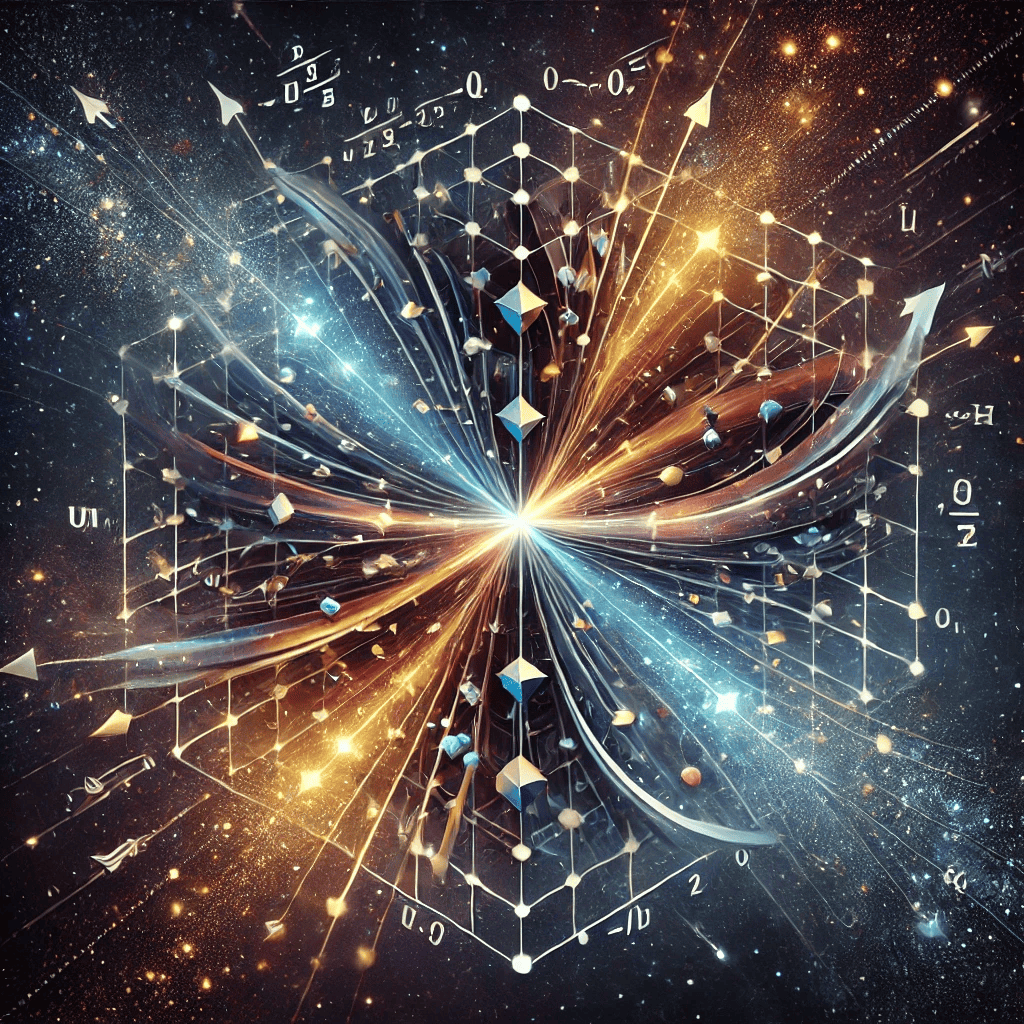
\includegraphics[width=0.8\textwidth]{jacobian.png}

    \caption{The Jacobian of the stress-energy tensor specifies the necessary information to describe energy flows in the brain.}
\end{figure}

\subsection{Coupling-interface Terms}

The coupling and interface terms in the stress-energy framework capture how different subsystems interact to maintain conscious coherence. These terms are essential for understanding how local energy dynamics combine into global conscious states.

For any two subsystems $\alpha$ and $\beta$, the coupling terms $C_{\mu\nu}(\alpha,\beta)$ can be expanded as:

$C_{\mu\nu}(\alpha,\beta) = \gamma(\alpha,\beta)[\partial_\nu\phi(\alpha)\partial_\mu\phi(\beta) - \eta_{\mu\nu}(\partial_\lambda\phi(\alpha)\partial^\lambda\phi(\beta))]$

\text{where:}
\begin{itemize}
\item $\gamma(\alpha,\beta)$ represents coupling strength
\item $\phi(\alpha)$, $\phi(\beta)$ are field variables for each subsystem
\item $\eta_{\mu\nu}$ is the metric tensor
\item $\partial_\lambda$ denotes covariant derivatives
\end{itemize}

The interface terms at boundaries $\partial \Omega$ take the form:

$B_{\mu\nu}(x) = \sigma(x)[n \cdot \nabla T_{\mu\nu}] + \kappa(x)T_{\mu\nu}|_{\partial\Omega}$

\text{where:}
\begin{itemize}
\item $\sigma(x)$ represents interface conductivity
\item $n$ is the unit normal to the boundary
\item $\kappa(x)$ captures boundary resistance
\end{itemize}

These terms must satisfy conservation conditions:

$\int_{\partial\Omega} B_{\mu\nu}(x)\,dS + \int_\Omega C_{\mu\nu}(\alpha,\beta)\,dV = 0$

This ensures energy and information flow continuously across subsystem boundaries while maintaining coherent conscious states.

The total dynamics at interfaces must also satisfy coherent boundary conditions:

$\sum_{\alpha,\beta} [C_{\mu\nu}(\alpha,\beta) + \partial_\lambda B_{\mu\nu}(\alpha,\beta)] \leq \eta(x,t)$

where $\eta (x,t)$ represents the maximum allowable local deviation from perfect coherence, constrained by thermodynamic considerations. These conditions ensure that energy transfers between subsystems remain within bounds that support conscious processing.

The complete interface dynamics can be expressed through a hierarchy of coupling terms:

$C_{\mu\nu} = C^{(1)}_{\mu\nu} + C^{(2)}_{\mu\nu} + C^{(3)}_{\mu\nu} + \cdots$

where each order captures increasingly complex interactions between subsystems, with higher-order terms typically decreasing in magnitude:

$|C^{(n)}_{\mu\nu}| \sim O(\gamma^n)$

where $\gamma < 1$ is a coupling parameter.

The mathematical foundations of stress-energy tensors and their applications to complex dynamical systems can be further explored through several seminal works. A comprehensive introduction to the geometric foundations is presented in \cite{Frankel2011}, which provides essential background on tensor analysis and differential geometry. The classic treatment in \cite{Misner1973} offers deep insights into how stress-energy tensors describe the flow and distribution of energy-momentum in physical systems, while \cite{Landau1987} provides crucial perspectives on how these concepts apply to continuous media and field theories. For those interested in the quantum aspects of energy flow and coherence, \cite{Peskin1995} develops the mathematical framework necessary for understanding field-theoretic approaches to information integration. The relationship between stress-energy tensors and general covariance principles is thoroughly examined in \cite{Wald1984}, providing important context for understanding how local energy conservation emerges from global symmetries. These texts collectively establish the mathematical rigor needed to apply stress-energy tensor analysis to complex biological systems like the brain, where multiple forms of energy flow must maintain coherent relationships across various scales.

\section{Triangulation and Mutual Recursion}

The maintenance of conscious coherence requires not only proper coupling between subsystems but also continuous feedback and adjustment across regions. This leads us to incorporate triangulation and mutual recursion into our mathematical framework. Let R(x,t) represent the recursive operator that describes how local states update based on neighboring regions:

$R(x,t): T(x,t) \rightarrow T(x,t + \delta t)$

where triangulation ensures that for any three regions $A$, $B$, and $C$:

$\|R(A \rightarrow B) \circ R(B \rightarrow C) - R(A \rightarrow C)\| < \varepsilon$

This formalism captures how conscious states maintain consistency through continuous mutual adjustment.

The unity of consciousness across spatially separated regions presents a fundamental challenge that ECC addresses through coordinated triangulation and recursive updating. For non-adjacent regions A and C, separated by intermediate regions {Bi}, consciousness maintains coherence through recursive triangulation chains:

$R(A \rightarrow C) = \circ_{i} R(B_i \rightarrow B_{i+1})$

where the composition of local recursive operators must satisfy the global coherence condition:

$\|R(A \rightarrow C) - R(A \rightarrow B_1) \circ R(B_1 \rightarrow B_2) \circ \cdots \circ R(B_n \rightarrow C)\| < \varepsilon(d)$

Here, $\varepsilon(d)$ represents the maximum allowable deviation as a function of distance d between regions.

The triangulation operators $T(x,y,z)$ acting on any three regions must satisfy:

1. Consistency across paths:
$T(A,B,C) \approx T(A,B',C)$

for any alternative intermediate point $B'$, where $"\approx"$ indicates agreement within coherence bounds.

2. Mutual recursion stability:
$R^{(n+1)}(x) = F[R^{(n)}(y) \mid y \in N(x)]$

where:

- $R(n)$ represents the nth recursive update

- $N(x)$ is the neighborhood of point $x$

- $F$ is the recursive update function

This framework enables non-local coherence maintenance through:

$\|T(A,B,C) - T(A,B',C)\| \leq \kappa \exp(-\lambda d)$

where $\kappa$ and $\lambda$ are constants determining how quickly coherence can propagate across distance $d$.

This non-local coherence maintenance is further constrained by the recursive coherence bound:

$\sum_{x,y} \|R^{(n+1)}(x) - F[R^{(n)}(y)]\| \leq \eta(t)\exp(-\mu d(x,y))$

where $\eta(t)$ represents time-dependent coherence thresholds and $\mu$ describes the spatial decay of coherence. The total system must satisfy both local and global stability conditions:

$\text{Local: } \|R^{(n+1)}(x) - R^{(n)}(x)\| \rightarrow 0 \text{ as } n \rightarrow \infty$

$\text{Global: } \|T(A,B,C) - T(A',B',C')\| \leq \varepsilon \text{ for any valid triangulation triple}$

These mathematical structures provide the foundation for understanding how consciousness maintains unity across spatial and temporal separations, leading us to consider how these local mechanisms combine to create global conscious states in the next section.

Several foundational works provide deeper insight into the mathematical principles underlying triangulation and mutual recursion in complex systems. The seminal work \cite{Bird1988} establishes crucial foundations for understanding recursive patterns in functional systems, particularly relevant to how neural networks maintain stable recursive relationships. A rigorous treatment of fixed-point theory for recursive queries is presented in \cite{Alegre2017}, offering mathematical tools essential for analyzing how recursive processes achieve stable states in biological systems. For understanding the network theoretical aspects of triangulation, \cite{Erdos1959} provides fundamental insights into random graph theory that inform how triangulated relationships emerge and stabilize in neural networks. The biological implications of recursive organization are thoughtfully explored in \cite{Maturana1987}, which examines how living systems maintain coherence through recursive interactions. Building on this, \cite{Freeman2000} offers crucial perspectives on how mesoscopic brain dynamics emerge from recursive processes and triangulated relationships across neural populations. The relationship between recursion and consciousness is further illuminated in \cite{Hofstadter2007}, which explores how self-referential loops and recursive processes might contribute to conscious experience. These works collectively provide the theoretical foundation necessary for understanding how triangulation and mutual recursion contribute to the maintenance of conscious states through coherent energy dynamics.

\section{Local-to-Global Coherence}

The integration of sheaf theory, stress-energy tensors, and recursive triangulation provides a comprehensive mathematical framework for understanding how consciousness achieves coherent global states from local dynamics. Let $M$ represent the manifold of possible conscious states. The global section $S \in F(M)$ emerges from the interplay of local coherence mechanisms through the coherence integration equation:

$S = \int_M [T_{\mu\nu} \circ R \circ T](x) \,dV$

where the composition of stress-energy dynamics ($T\mu\nu$), recursive updates ($R$), and triangulation operators ($T$) must satisfy both local and global coherence conditions.

The global coherence of consciousness emerges from the satisfaction of multiple simultaneous constraints across all mathematical structures previously introduced:

1. Sheaf Coherence:
$\forall U,V \subseteq M: \rho_{U \cap V}(S|_U) = \rho_{V \cap U}(S|_V)$

2. Energy Conservation:
$\partial_\sigma T_{\mu\nu} + \sum_{\alpha,\beta} C_{\mu\nu}(\alpha,\beta) = 0$

3. Recursive Stability:
$\lim_{n \rightarrow \infty} \|R^{(n+1)} - R^{(n)}\| \rightarrow 0$

4. Triangulation Consistency:
$\sup_{A,B,C} \|T(A,B,C) - T(A',B,C)\| \leq \varepsilon$

These conditions must be simultaneously satisfied while maintaining thermodynamic efficiency:

$\eta = -\int_M T_{\mu\nu}\partial_\mu\xi_\nu \,dV \leq \eta_{\text{max}}$

where $\xi_\nu$ represents the Killing vector fields associated with energy conservation.

This mathematical framework, while abstract, finds direct physical implementation in biological neural systems. The translation from mathematical formalism to biological reality requires understanding how these structures are realized through specific biophysical mechanisms.

For deeper exploration of local-to-global coherence in neural systems, several foundational works provide crucial theoretical frameworks. The seminal work in \cite{Sporns2011} establishes fundamental principles for understanding how local neural dynamics integrate into global brain states through network organization. A rigorous treatment of coordination dynamics is presented in \cite{Bressler2016}, offering essential insights into how local neural populations achieve coherent relationships across multiple scales. The theoretical framework in \cite{Kelso2012} provides crucial perspectives on multistability and metastability in brain dynamics, particularly relevant to understanding how local coherence patterns contribute to global conscious states. Building on these foundations, \cite{Werner2013} examines consciousness through the lens of phase space dynamics and criticality, offering important insights into how local-to-global transitions emerge in neural systems. The relationship between electromagnetic field integration and consciousness is thoughtfully explored in \cite{McFadden2020}, which examines how local field potentials might contribute to global conscious integration. These perspectives are complemented by \cite{Tononi2015}, which provides a theoretical framework for understanding how information integration occurs across different scales in conscious systems. Collectively, these works establish the theoretical foundations necessary for understanding how local patterns of neural activity combine to create globally coherent conscious states through multiple mechanisms of integration and coordination.

Drawing from recent theoretical work in cognitive neuroscience and complex systems, coherence within Energetically Coherent Computing (ECC) represents a fundamental organizing principle that emerges from the coordinated interaction of multiple energy forms across neural systems. This coherence manifests through the synchronized integration of electromagnetic fields, ionic gradients, and metabolic processes that collectively give rise to conscious experience \cite{McFadden2020, Werner2013}.

The framework of coherence in ECC can be understood through several interconnected dimensions. At the physical level, coherence emerges from the synchronized alignment of energy flows across multiple spatial and temporal scales. This alignment enables large-scale integration while maintaining local specificity, creating conditions necessary for conscious processing \cite{Kelso2012}. The resulting patterns of energy organization demonstrate remarkable stability while preserving the flexibility required for adaptive response to changing conditions \cite{Freeman2007}.

From an informational perspective, coherence enables the integration of diverse neural processes into unified conscious states. This integration occurs through carefully orchestrated patterns of energy flow that maintain consistent relationships across sensory, cognitive, and motor systems \cite{Baars2007}. The resulting coherent states provide the foundation for the phenomenal unity of consciousness while enabling sophisticated information processing \cite{Tononi2015}.

The mathematical formalization of coherence through sheaf theory provides rigorous tools for understanding how local patterns of energy organization combine into global conscious states \cite{Rushworth2018}. This approach reveals how disruptions in coherence can lead to altered states of consciousness, whether through sleep, anesthesia, or pathological conditions. The sheaf-theoretic framework particularly illuminates how consciousness requires proper "gluing" of local coherent states across neural tissues \cite{Abramsky2008}.

Coherence in ECC also reflects fundamental principles of energetic efficiency, where neural systems achieve sophisticated information processing while minimizing unnecessary energy dissipation \cite{Dehaene2011}. This efficiency emerges through evolved patterns of organization that enable both stability and adaptability while respecting thermodynamic constraints \cite{Bressler2016}. The resulting balance between energy conservation and information processing capacity proves essential for maintaining conscious states.

The dynamic nature of coherent organization becomes particularly evident through coordination dynamics \cite{Kelso2012}. Rather than representing static patterns, coherence emerges from continuous processes of self-organization that maintain stability while enabling flexible response to changing conditions. This dynamic stability allows consciousness to persist through varying environmental demands while preserving essential organizational features \cite{Haken2012}.

Understanding coherence through ECC thus reveals fundamental principles about how consciousness emerges from physical processes while remaining grounded in rigorous mathematical formalism. This framework suggests new approaches to investigating consciousness while providing theoretical tools for understanding both normal function and pathological conditions \cite{Alexander2019}. The resulting synthesis bridges phenomenology and physics through careful attention to the organizing principles that enable conscious experience.

After establishing this mathematical framework for describing patterns of energetic coherence across multiple scales, we come to a fundamental insight: what emerges from these formalisms is not merely a description of energy dynamics, but a deep theory of computation itself. Computation lies at the heart of ECC - not as abstract symbol manipulation, but as physically embodied processes maintaining specific patterns of energetic coherence.

The mathematical tools developed above - from sheaf-theoretic models of local-to-global integration to the analysis of coherent energy flows through stress-energy tensors - reveal how biological systems achieve sophisticated information processing while remaining bound by physical constraints. This suggests a radical reconceptualization of computation itself, one that maintains rigorous connections to physical dynamics rather than abstracting away from them.

This naturally leads us to examine a fundamental question: What is computation? While traditional approaches treat computation as substrate-independent symbol manipulation, ECC suggests a different view - one where computation emerges from and remains inseparable from coherent physical processes. Understanding this distinction requires us to carefully examine our basic assumptions about the nature of computation itself in the next section.

\section{What is Computation?}

The classical theory of computation, developed through pioneering work on effective procedures and mechanical calculation, established computation as the manipulation of discrete symbols according to formal rules \cite{Turing1936}. However, ECC suggests that consciousness requires a fundamentally different kind of computation—one grounded in continuous, physically embodied energy flows rather than abstract symbol manipulation \cite{MacLennan2004}.

Traditional computational theory centers on the notion that any computation can be reduced to a sequence of simple, mechanical steps executed by an abstract machine \cite{Copeland2017}. The universal Turing machine demonstrated that all classical computation could be realized through the manipulation of discrete symbols on an infinite tape. The Church-Turing thesis suggested that any intuitively computable function could be computed by these equivalent formalisms, establishing a foundational principle for computer science \cite{Smith2002}.

However, these classical approaches share crucial assumptions that ECC challenges. First, they presume that information can be perfectly encoded in discrete states, while ECC argues that conscious processing requires continuous, analog-like states that cannot be \textbf{fully} captured by discrete representations \cite{vanGelder1995}. Second, the Church-Turing thesis implies that computation is independent of its physical implementation, whereas ECC contends that consciousness requires specific physical properties and energy dynamics that cannot be abstracted away \cite{Landauer1996}.

These theoretical tensions highlight fundamental questions about the nature of computation itself. While the Church-Turing thesis may capture the essence of abstract symbol manipulation, consciousness appears to require what \cite{Piccinini2015} terms natural computation—physically embodied processes that cannot be reduced to discrete symbolic operations. This suggests that understanding consciousness requires expanding our conception of computation beyond traditional algorithmic frameworks.

\begin{figure}[h]
    \centering
    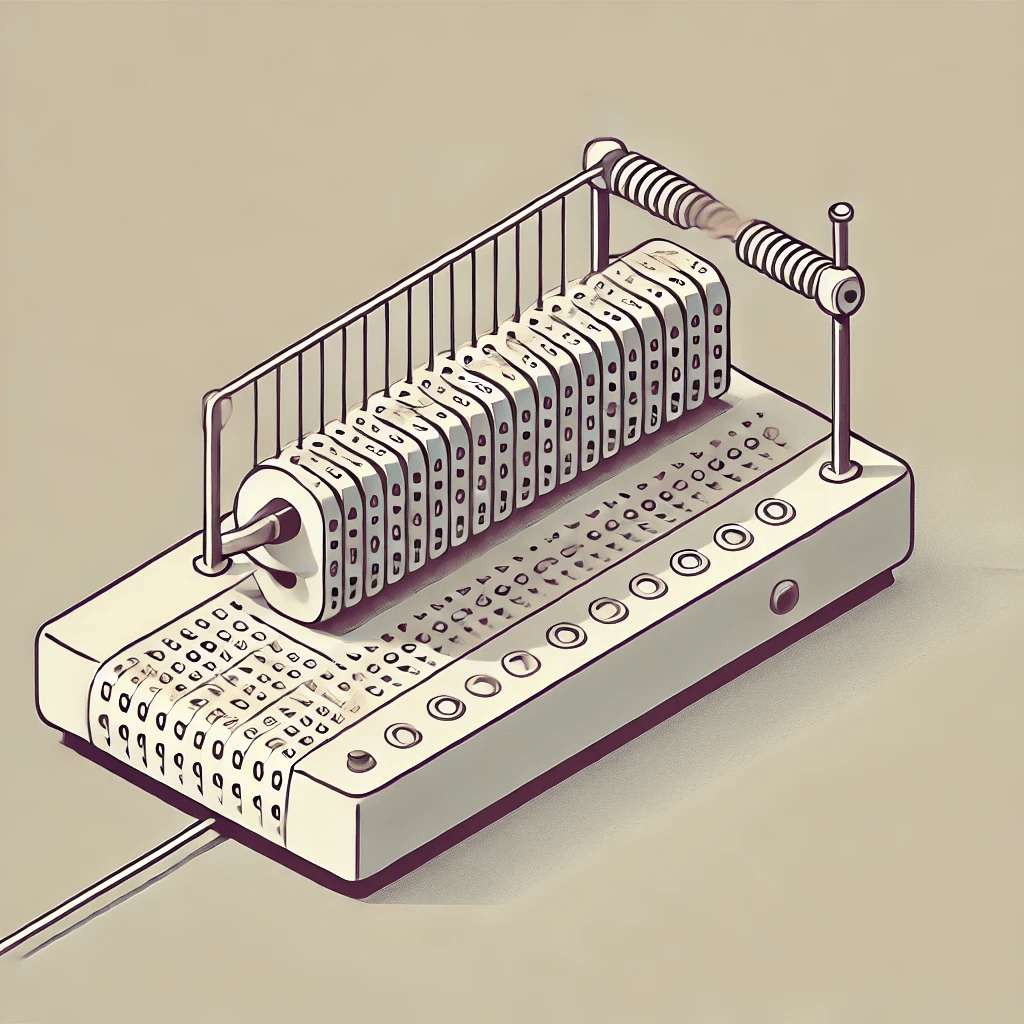
\includegraphics[width=0.8\textwidth]{turing.png}

    \caption{Artwork depicting a simple realization of an abstract Turing machine}
\end{figure}

The relationship between physical implementation and computation takes on particular significance in ECC's framework. While traditional computational theory treats physical substrates as incidental to computational processes \cite{Chalmers2011}, ECC suggests that certain physical properties—particularly those enabling coherent energy flows—are essential to conscious computation \cite{Landauer1996}. This perspective aligns with emerging understanding of how biological systems process information through continuous, physically grounded dynamics rather than discrete state transitions.

Recent theoretical work has begun to challenge the assumption that all natural processes admit computational description \cite{Searle1990}. Just as digestion cannot be adequately characterized as information processing, and gravitational phenomena cannot be reduced to computation, conscious experience may emerge from physical dynamics that resist computational abstraction \cite{vanGelder1995}. This aligns with growing skepticism about the computational theory of mind, particularly regarding the context-sensitivity and holistic nature of conscious thought.

TODO: G Ryle cite on category error below?

The framework suggests that attempting to reduce consciousness to computation represents what \cite{Smith2002} identifies as a category error—confusing the abstract map of computational description with the physical territory of conscious experience. While computational models may capture certain aspects of cognitive processing, they fundamentally miss the continuous, field-like properties that characterize conscious experience \cite{Piccinini2015}. This limitation becomes particularly evident when considering how consciousness maintains coherence across distributed neural processes.

Traditional computationalism faces particular challenges in explaining the temporal dynamics of consciousness \cite{Siegelmann2003}. The continuous flow of conscious experience appears fundamentally at odds with the discrete state transitions that characterize classical computation. ECC suggests that this temporal continuity emerges naturally from the physical dynamics of coherent energy flows, rather than requiring additional computational mechanisms to bridge discrete states.

The implications extend beyond theoretical understanding to practical questions about artificial consciousness \cite{Aaronson2013}. While digital computers excel at manipulating discrete symbols according to formal rules, they may be fundamentally incapable of supporting the specific forms of energetic coherence that ECC identifies as essential to conscious experience. This suggests that creating conscious artificial systems might require radically different approaches to computation and physical implementation.

The distinction between classical computation and conscious processing becomes particularly evident when examining how biological systems maintain coherent states across multiple scales \cite{MacLennan2004}. Unlike digital computers that maintain sharp boundaries between processing elements, conscious systems operate through continuous fields of influence that span multiple levels of organization. The resulting integration cannot be achieved through discrete computational steps but requires physical processes that maintain coherence through direct energetic interaction.

This perspective suggests a fundamental revision of how we understand computation in biological systems \cite{Adriaans2013}. Rather than viewing neural computation as analogous to digital processing, ECC proposes that conscious systems compute through patterns of energetic coherence that enable both stability and flexibility. This aligns with emerging views in theoretical neuroscience that emphasize the importance of continuous, dynamical processes in neural computation \cite{Piccinini2015}.

Recent work has begun to formalize these distinctions through mathematical frameworks that capture the continuous, field-like properties of conscious processing \cite{Siegelmann2003}. These approaches suggest that conscious computation operates in a fundamentally different regime from classical digital computation, one characterized by coherent energy flows rather than discrete state transitions. This mathematical perspective helps explain why consciousness exhibits properties that appear difficult or impossible to replicate through traditional computational approaches.

The relationship between energy and information takes on particular significance in this context \cite{Landauer1996}. While classical computation treats information as abstract and substrate-independent, ECC suggests that conscious processing requires specific physical implementations that enable particular patterns of energy flow and transformation. This perspective aligns with fundamental insights about the physical nature of information while suggesting new approaches to understanding how conscious systems process and integrate information.

The framework also provides insight into why certain aspects of conscious experience appear resistant to computational modeling \cite{Searle1990}. Features such as qualitative experience, temporal continuity, and global integration may emerge naturally from the physical dynamics of conscious systems while remaining fundamentally irreducible to discrete computational processes. This suggests that understanding consciousness requires moving beyond purely computational approaches to consider the physical basis of conscious experience.

This reconceptualization of computation through ECC's framework raises fundamental questions about the nature of conscious processing \cite{Wheeler1990}. While traditional approaches treat consciousness as emerging from abstract information processing, ECC suggests that conscious experience requires specific forms of physical organization that enable coherent energy dynamics. This perspective helps explain both the remarkable capabilities of conscious systems and their fundamental limitations.

The relationship between computation and physical implementation becomes particularly significant when considering the temporal aspects of conscious processing \cite{Deutsch2011}. Unlike classical computation, which proceeds through discrete time steps, consciousness exhibits continuous temporal evolution that emerges from the physical dynamics of neural systems. This temporal continuity appears essential to conscious experience yet proves difficult or impossible to capture through traditional computational frameworks.

Recent theoretical work has begun to explore how physical constraints shape the computational capabilities of conscious systems \cite{Fodor1981}. Rather than viewing these constraints as limitations to be overcome, ECC suggests they play a constructive role in enabling the specific forms of computation necessary for consciousness. This perspective aligns with emerging understanding of how biological systems achieve sophisticated information processing through their physical organization \cite{Smith2002}.

The framework provides particular insight into the relationship between local and global aspects of conscious computation \cite{vanGelder1995}. While traditional computational approaches often struggle to explain how distributed processing gives rise to unified experience, ECC suggests that this integration emerges naturally from the physical dynamics of coherent energy flows. This helps explain how consciousness achieves both differentiated processing and global coherence without requiring additional computational mechanisms.

These theoretical insights have important implications for understanding both biological consciousness and artificial systems \cite{Piccinini2015}. While digital computers may excel at certain forms of information processing, they appear fundamentally limited in their ability to support the specific types of computation that ECC identifies as essential to consciousness. This suggests that creating conscious artificial systems might require radically different approaches to computation and physical implementation.

The distinction between classical and conscious computation illuminates fundamental questions about the nature of mind and experience \cite{Chalmers2011}. ECC suggests that consciousness represents a unique form of physical computation that cannot be reduced to abstract symbol manipulation or discrete state transitions. This perspective helps resolve longstanding debates about the relationship between computation and consciousness while suggesting new directions for research and development.

The apparent tension between ECC's non-computational account of consciousness and its retention of "computation" in its name resolves through careful consideration of how the framework redefines computation itself \cite{MacLennan2004}. Rather than rejecting computation entirely, ECC reconceptualizes it as emerging from physical dynamics that maintain specific patterns of energetic coherence. This broadened understanding of computation aligns with recent theoretical work suggesting that biological systems compute through continuous, physically-grounded processes rather than discrete symbolic operations \cite{Siegelmann2003}. ECC accepts that consciousness implies computation but not vice versa. Thus, we conecptualize consciousness as computationally adjacent - correlated with but not caused by computation per se.

This theoretical synthesis has important implications for both cognitive science and artificial intelligence \cite{Deutsch2011}. While traditional computational approaches have yielded significant insights into many aspects of cognition, consciousness appears to require forms of physical computation that go beyond classical frameworks. Understanding these distinctions may prove crucial for developing artificial systems that could potentially support conscious-like processing \cite{Aaronson2013}.

The framework thus suggests a fundamental revision in how we understand the relationship between computation and consciousness \cite{Wheeler1990}. Rather than treating consciousness as an emergent property of abstract computation, ECC positions it as arising from specific forms of physical computation that maintain coherent energy dynamics across multiple scales. This perspective provides new insights into both the possibilities and limitations of conscious systems while suggesting productive directions for future research and development \cite{Landauer1996}.

\newpage
\section{References}
\printbibliography[title={},heading=subbibliography]
%\printbibliography[title={References: Theoretical Framework}]
\end{refsection}

\section*{\phantom{Part V Biological Implementation}}
\h{Biological Implementation}

\begin{refsection}[references/0001_3_bio_implementation.bib]

\section{Biophysics}

The abstract mathematical structures described above take concrete form in the brain through specific biophysical mechanisms. From protein conformational changes to electromagnetic field interactions, from astrocytic calcium waves to gap junction coupling, the brain implements these mathematical principles through precisely organized biological structures. Understanding this implementation requires examining how physical processes at multiple scales combine to create the conditions necessary for conscious processing.

The translation of ECC's mathematical framework into biological reality occurs through specific physical mechanisms operating across multiple scales of neural organization. These biophysical implementations must satisfy both the mathematical constraints required for conscious coherence and the practical limitations imposed by biological systems.

At the molecular scale, protein conformational dynamics implement aspects of the rich alphabet through energetically-indexed states. These conformational changes follow the mathematical principles of our framework through:

$\Delta G = \Delta H - T\Delta S$

where:

- $\Delta G$ represents the free energy change of protein transitions

- $\Delta H$ captures enthalpic contributions from molecular interactions

- $T \Delta S$ represents entropic terms affected by temperature and disorder

Moving to larger scales, electromagnetic fields emerge from coordinated cellular activity, implementing aspects of the field coherence terms in our tensor framework:

\begin{align}
\nabla \cdot \mathbf{E} &= \frac{\rho}{\varepsilon_0} \\
\nabla \times \mathbf{B} &= \mu_0(\mathbf{J} + \varepsilon_0\frac{\partial \mathbf{E}}{\partial t})
\end{align}

where these Maxwell equations describe how charge distributions ($\rho$) and currents ($J$) create the electromagnetic fields that help maintain conscious coherence.

The energetic constraints on neural signaling reveal remarkable optimization for both efficiency and reliability \cite{Attwell2001}. Neural tissues must carefully balance the energy demands of maintaining ion gradients and supporting synaptic transmission against the metabolic costs of protein synthesis and cellular maintenance \cite{Harris2012}. These biophysical constraints shape how conscious processing emerges from neural activity while determining fundamental limits on information processing capacity.

The interaction between neurons and astrocytes demonstrates sophisticated mechanisms for managing energy distribution across neural tissues \cite{Hertz2007}. Through coordinated regulation of glucose uptake, lactate shuttling, and ion homeostasis, these cellular networks achieve remarkable efficiency in matching energy supply to computational demands \cite{Magistretti2015}. This bioenergetic coupling proves essential for maintaining the coherent states necessary for conscious processing.

\subsection{Bioenergetics}

This brings us to consider how the brain manages its energy economy to support these biophysical processes. Bioenergetics provides the crucial link between abstract mathematical requirements for coherence and their physical implementation through metabolic processes. The central role of ATP as cellular energy currency implements key aspects of our stress-energy tensor framework through chemiosmotic coupling and oxidative phosphorylation \cite{Mitchell1961}.

The brain's bioenergetic implementation of ECC's framework operates through tightly coupled energy transformation cascades. At the molecular level, this coupling is described by the chemiosmotic equation \cite{Nicholls2013}:

$\Delta G = -nF(\Delta \Psi + \frac{RT}{F}\ln\frac{[H^+]_{\text{out}}}{[H^+]_{\text{in}}})$

\text{where:}
\begin{itemize}
\item $\Delta \Psi$ represents the membrane potential
\item $F$ is Faraday's constant
\item $n$ represents the number of protons transported
\item $R$ is the gas constant
\item $T$ is temperature
\end{itemize}

These molecular energy transformations must satisfy both local efficiency constraints and global coherence requirements through the bioenergetic coupling tensor:

$B_{\mu\nu} = \begin{bmatrix} 
\text{ATP}\rightarrow\text{ADP} & \text{H}^+\text{gradient} \\
\text{NAD}^+\text{/NADH} & e^-\text{transport}
\end{bmatrix}$

The coupling between these processes must maintain specific ratios \cite{Rolfe1997}:

\begin{align}
\text{P/O ratio} &\approx 2.5 \text{ (glucose oxidation)} \\
\text{P/O ratio} &\approx 1.5 \text{ (fatty acid oxidation)}
\end{align}

The brain demonstrates remarkable specialization in its metabolic organization compared to other tissues \cite{Berndt2012}. Neural energy management requires sophisticated compartmentalization between different cell types and subcellular domains \cite{Shulman2004}. This creates what has been termed metabolic compartmentation - the precise spatial organization of energetic processes that enables both efficient energy utilization and maintained coherence across neural networks.

Glucose transport and utilization reveal particularly sophisticated regulation in neural tissues \cite{Szablewski2017}. The precise control over glucose uptake and metabolism, coupled with the astrocyte-neuron lactate shuttle, creates an integrated system for matching energy supply to computational demands \cite{Pellerin2012}. This metabolic architecture enables neural circuits to maintain coherent processing while adapting to changing energy requirements.

\subsection{Neuroenergetics}

The transition from general bioenergetics to neuroenergetics reveals unique features of brain energy management. Unlike other tissues, the brain must maintain continuous, stable energy flows while allowing for rapid local adjustments \cite{DiNuzzo2017}. This creates a neuroenergetic paradox - the need to maintain both stability and flexibility in energy distribution. The solution involves sophisticated mechanisms of energy delivery and utilization that implement our mathematical framework through specific biological processes.

The brain's unique energy requirements necessitate sophisticated mechanisms for maintaining an energetic reserve capacity while enabling rapid redistribution. This manifests through the astrocyte-neuron lactate shuttle (ANLS), which implements aspects of our coupling terms through metabolic compartmentalization \cite{Pellerin2012}. 

Neurons maintain high oxidative capacity but limited glucose utilization, while astrocytes demonstrate high glycolytic capacity with glucose uptake that exceeds their oxidative requirements \cite{Magistretti2015}. This division creates an energetic buffer system that supports both stable baseline activity and rapid responses to changing demands. The continuous management of these energy flows must satisfy both local metabolic constraints and global coherence requirements specified in our mathematical framework.

The spatial organization of neuroenergetic systems demonstrates remarkable optimization for both efficiency and reliability \cite{Attwell2001}. Through precise arrangement of mitochondria, careful regulation of glucose transporters, and sophisticated control over neurotransmitter recycling, neural tissues achieve extraordinary efficiency in matching energy supply to computational demands \cite{Harris2012}. This architectural efficiency proves essential for maintaining coherent conscious states while enabling rapid adaptation to changing conditions.

Critically, neuroenergetics reveals how the brain implements the theoretical requirements for consciousness through specific biological mechanisms \cite{Hertz2007}. The precise spatial and temporal control of energy delivery, coupled with sophisticated mechanisms for waste removal and heat management, creates the conditions necessary for maintaining coherent conscious states while operating within biological constraints.

\section{Neural Architecture}

The implementation of ECC's principles through bioenergetic mechanisms depends critically on the brain's underlying structural organization. Neural architecture provides the physical substrate that enables both efficient energy distribution and the maintenance of coherent conscious states. This organization reflects evolutionary optimization for both information processing and energy management, creating what can be described as structured efficiency in biological systems \cite{Hilgetag2020}.

The layered organization of the cortex serves as an ideal physical structure for implementing ECC's principles of energetic coherence and information integration \cite{Douglas2004}. The distinct laminar organization, with its carefully regulated ratios of excitatory and inhibitory neurons, establishes coherence domains - regions where energy flows can be locally stabilized while maintaining dynamic coupling with adjacent areas \cite{Harris2015}.

Cortical columns emerge as particularly significant architectural features, forming natural units for maintaining local energetic coherence \cite{Mountcastle1997}. These columns, extending vertically through cortical layers, create coherence channels that enable several crucial functions. They facilitate efficient vertical integration of information across cortical layers while providing contained units for local stabilization of energy dynamics. The balanced ratios of excitation and inhibition within these columns help maintain low-entropy states, while their structure creates natural boundaries for the sheaf-theoretic sections described in the mathematical formalism.

The horizontal organization of cortical tissue proves equally important, with its dense network of lateral connections forming coherence coupling zones \cite{DeFelipe2011}. These zones enable the propagation of coherent states between adjacent columns and support the distribution of energy loads across the cortical sheet. This horizontal architecture implements the \textit{gluing} operations described in the sheaf-theoretic framework while enabling the creation of larger-scale coherent fields from local stable states.

White matter architecture plays an essential role beyond mere connectivity \cite{Sporns2011}. Long-range fiber tracts serve as coherence bridges that help maintain global stability of conscious states. The precise topology of these connections appears to reflect evolutionary optimization for both minimal wiring length, reducing energy costs, and maximal maintenance of coherent fields across distributed regions. This architectural efficiency directly supports ECC's emphasis on low-entropy conscious states emerging from coherent energy dynamics.

Perhaps most crucial is the neuropil itself - the dense network of neural processes, glial cells, and extracellular matrix that fills the spaces between neuronal cell bodies \cite{Kasthuri2015}. This intricate mesh, supported by dendritic processes and their spines, creates the physical substrate necessary for maintaining coherent energy states and enabling state sharing across regions. The neuropil's architecture proves particularly well-suited for supporting brain waves, which ECC views as essential mechanisms for maintaining coherent states. Its dense connectivity and precise spatial organization allows for efficient propagation of oscillatory activity, local synchronization of neural populations, and the creation of standing waves that help stabilize conscious states.

\begin{figure}[h]
    \centering
    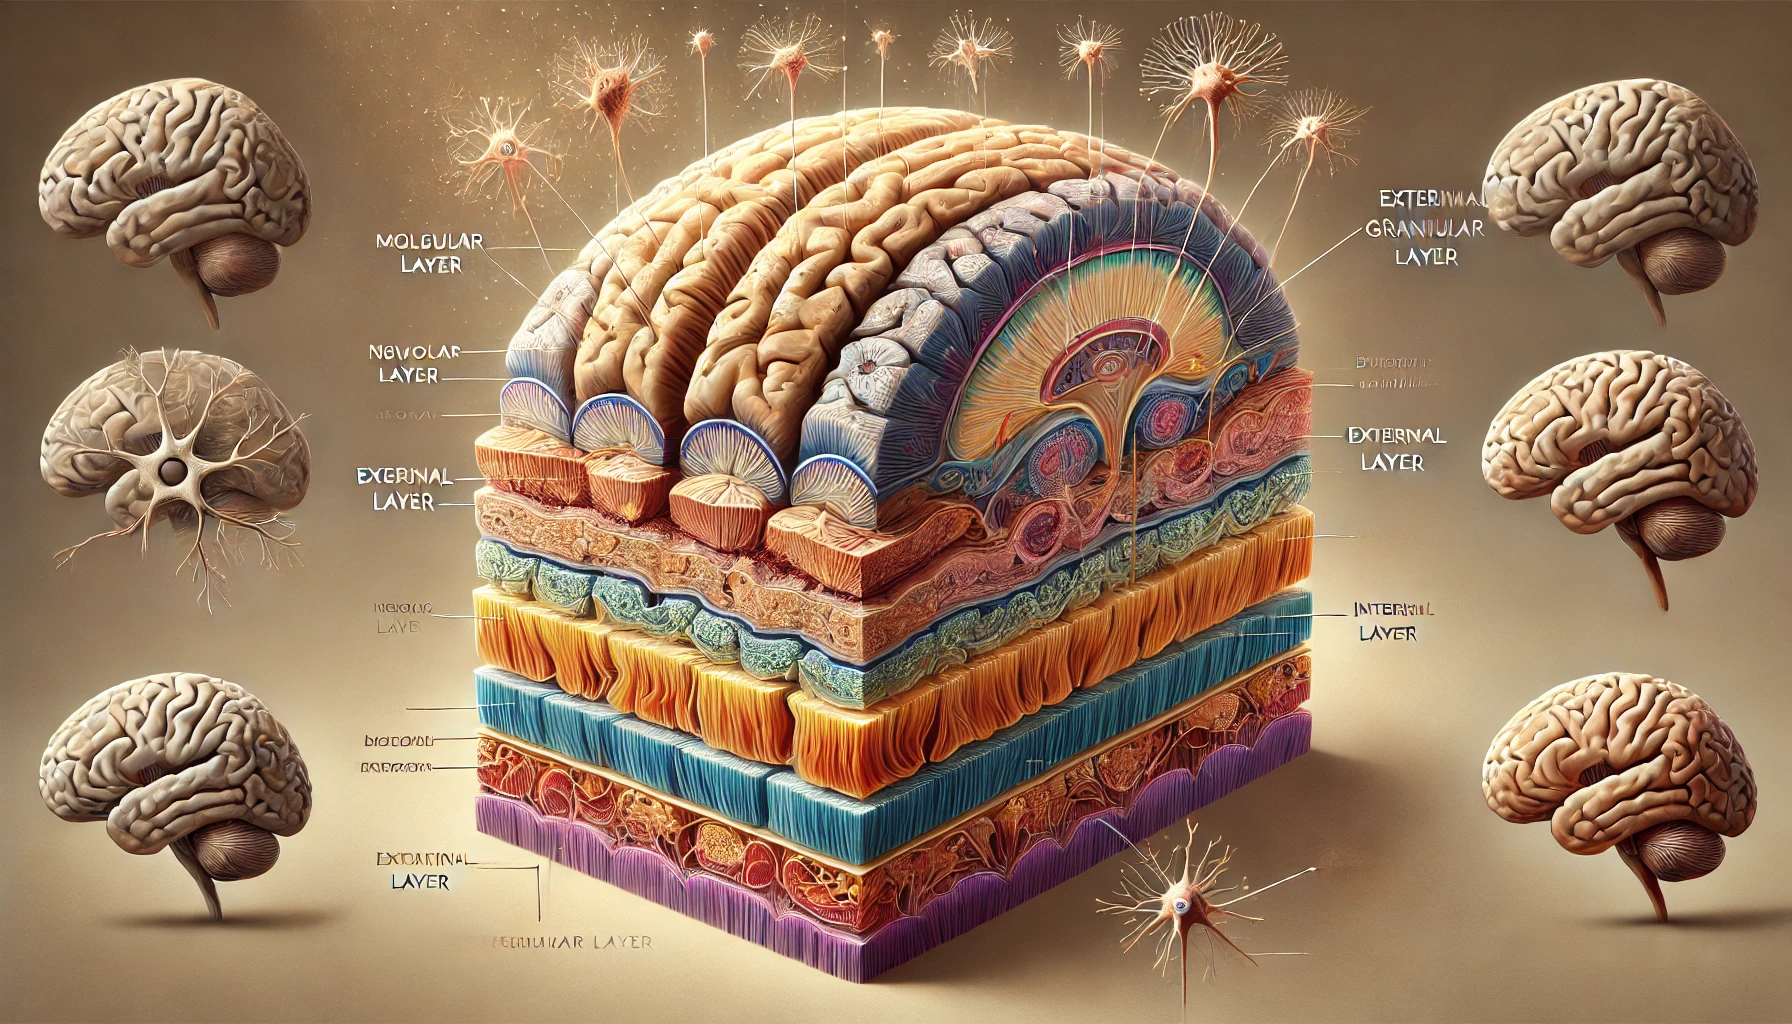
\includegraphics[width=0.8\textwidth]{cortical_layers.png}

    \caption{Cortical layers}
\end{figure}

The neuropil's dense connectivity serves multiple critical functions in maintaining conscious states \cite{Kasthuri2015}. Through its precise spatial organization, it enables coordinated interactions between neurons and glia while providing structured pathways for field-like effects to propagate. The arrangement of cellular processes creates an intricate three-dimensional matrix that supports both local processing and global integration of neural activity.

Astrocytic processes within the neuropil form an essential component of this architecture \cite{Peters1984}. Their elaborate branching patterns and strategic positioning allow them to monitor and modulate synaptic activity while maintaining ion homeostasis across substantial volumes of neural tissue. This spatial organization enables astrocytes to coordinate energy distribution and maintain coherent states across multiple spatial scales.

The extracellular matrix embedded within the neuropil provides another crucial architectural element \cite{Braitenberg1998}. Its molecular scaffolding helps stabilize synaptic connections while influencing the diffusion of neurotransmitters and ions. The precise composition and organization of the matrix varies across brain regions, creating specialized microenvironments that support different aspects of neural processing and energy management.

Dendritic architecture within the neuropil deserves particular attention \cite{Rockland2020}. The intricate branching patterns of dendrites create overlapping fields of integration that allow neurons to sample inputs from diverse sources while maintaining specific computational properties. This architectural feature enables sophisticated information processing while supporting the establishment of coherent energy states across neural populations.

The spatial arrangement of synaptic connections within the neuropil reflects both specific computational requirements and energy efficiency constraints \cite{Markram2015}. Synapses cluster in patterns that minimize wiring length while maximizing information transfer, creating local processing units that can maintain stable energy states while remaining dynamically responsive to changing inputs. This organization supports the emergence of coherent activity patterns while enabling flexible reconfiguration based on computational demands.

Gap junctions between cells provide another essential architectural feature within the neuropil \cite{Zeng2017}. These direct cellular connections create alternative pathways for signal propagation and state sharing, enabling rapid synchronization of cellular assemblies without requiring synaptic transmission. The distribution and regulation of gap junctions helps establish domains of coordinated activity that can maintain coherent states across multiple spatial scales.

The integration of these various architectural elements - astrocytic processes, extracellular matrix, dendritic fields, synaptic clusters, and gap junctions - creates a physical substrate capable of supporting the sophisticated energy dynamics required for conscious processing \cite{Bassett2017}. This multi-scale organization enables both local specialization and global integration while maintaining the energetic efficiency necessary for sustained conscious activity.

Through this architectural organization, the brain achieves a remarkable balance between stability and flexibility \cite{Buzsaki2006}. The structured pathways for energy flow and information processing allow for the maintenance of coherent states while enabling dynamic responses to changing conditions. This sophisticated architecture, refined through evolution, provides the physical foundation necessary for consciousness to emerge from organized energy flows within neural tissue.

The architectural organization of neural tissue culminates in a system that supports multiple modes of information transmission and energy propagation \cite{VanEssen2018}. Beyond classical synaptic transmission, the neuropil's structure enables ephaptic coupling, volume transmission, and field effects that contribute to conscious processing. These various mechanisms operate simultaneously across different spatial and temporal scales, creating a rich landscape of possible interactions that support coherent conscious states.

The evolutionary refinement of this architecture reflects a delicate balance between competing demands \cite{Hilgetag2020}. The need for efficient information processing must be weighed against energy constraints, while requirements for stability must accommodate the need for plasticity and adaptation. The resulting structure represents a sophisticated solution to these competing pressures, enabling conscious processing through carefully organized patterns of energy flow.

Perhaps most remarkably, this neural architecture creates conditions for emergent properties that transcend the capabilities of individual components \cite{vonBartheld2016}. Through its precise organization across multiple scales, from molecular arrangements to global connectivity patterns, the brain's structure enables the emergence of conscious experience from coherent energy dynamics. This emergence depends not just on the properties of individual elements but on their precise spatial arrangement and coordinated interaction.

Understanding neural architecture through the lens of ECC provides crucial insights into both the possibilities and constraints of conscious processing. The physical structure of neural tissue determines what patterns of energetic coherence can be maintained, what forms of information processing are possible, and what limitations must be respected. This architectural foundation proves essential for any complete theory of consciousness.

\section{Brain Waves}

Building on the neural architecture's structural foundation, brain waves emerge as primary mechanisms for implementing ECC's principles of state sharing and coherence maintenance. These oscillatory patterns, propagating through the neuropil's structured pathways, enable energetic coherence through tightly coupled state sharing across cortical regions \cite{Buzsaki2004}. Unlike digital computers with their discrete state transitions, brain waves support continuous, field-like properties that better align with ECC's emphasis on coherent energy flows and dynamic stability.

Different frequency bands serve complementary functions in maintaining conscious coherence \cite{Wang2010}. Gamma oscillations enable precise local synchronization, creating tight coupling between adjacent neural populations. Beta rhythms facilitate intermediate-range coordination between functional areas, while alpha waves help regulate larger-scale integration and inhibition. Theta oscillations support memory integration and emotional processing, and delta rhythms contribute to global state regulation \cite{Steriade2006}. These frequency bands do not operate in isolation but form nested hierarchies of coordination, where higher-frequency local oscillations become phase-locked to slower rhythms, creating cross-frequency coherence that enables integration across different spatial and temporal scales \cite{Canolty2010}.

The neuropil's architecture supports wave propagation through several sophisticated mechanisms \cite{Buzsaki2006}. Local circuit organization creates resonant structures that can sustain oscillatory patterns, while gap junctions between interneurons enable rapid synchronization of local populations. Astrocytic networks modulate wave propagation and help maintain stability, and the extracellular matrix provides a structured medium that shapes wave dynamics. These mechanisms work together to create and maintain patterns of coherent activity essential for conscious processing.

Brain waves serve multiple crucial functions in implementing ECC's principles \cite{Varela2001}. They enable efficient distribution of information across regions while supporting the maintenance of coherent states through oscillatory synchronization. Through careful management of energy flows, waves provide an efficient mechanism for coordinating activity across distributed neural populations. Different frequency bands help define functional boundaries between conscious states while enabling smooth transitions between them.

The interaction between brain waves and the neuropil's architecture creates coherence fields - stable patterns of energy flow that support conscious processing while maintaining thermodynamic efficiency \cite{Fries2015}. These fields provide the physical basis for the mathematical structures described in ECC's formal framework, enabling both local processing and global integration through continuous, field-like interactions.

Perhaps most remarkably, brain waves demonstrate how neural systems can maintain coherent states while enabling dynamic reorganization \cite{Engel2001}. During transitions between conscious states, wave patterns shift in coordinated ways that preserve overall coherence while allowing for rapid reconfiguration of neural activity. This capacity for stable yet flexible organization proves essential for maintaining conscious experience in the face of constantly changing environmental demands.

The coordination between brain waves and astrocytic networks deserves particular attention. While neurons generate the primary oscillatory patterns, the stability and propagation of these waves rely heavily on the regulatory influence of astrocytes \cite{Ward2003}. Brain waves propagating through the neuropil interact continuously with astrocytic networks, which help maintain proper conditions for coherent activity by regulating ion concentrations in the extracellular space, modulating synaptic transmission, coordinating metabolic support, and buffering excessive activity.

This sophisticated interaction between neuronal oscillations and glial regulation creates the conditions necessary for maintaining coherent conscious states while enabling dynamic responses to changing conditions \cite{Basar2013}. The resulting system demonstrates how biological organization can achieve both stability and flexibility through carefully orchestrated patterns of energy flow.

The relationship between brain waves and conscious experience reveals itself through multiple complementary mechanisms \cite{Jensen2007}. Oscillatory patterns create temporal windows for information integration, enabling distributed neural populations to coordinate their activity with precise timing. These windows of synchronization allow for the binding of sensory inputs, the coordination of motor outputs, and the integration of internal states into coherent conscious experiences.

The hierarchical organization of brain waves proves particularly significant for consciousness \cite{Lisman2013}. Slower oscillations modulate the amplitude of faster rhythms, creating nested patterns of activity that support both local processing and global integration. This cross-frequency coupling enables the brain to maintain multiple simultaneous processes while preserving overall coherence. For instance, theta rhythms may organize sequences of gamma-band activity, creating structured packages of information processing that can be integrated into broader conscious experiences.

Wave propagation through neural tissue demonstrates remarkable sophistication in managing energy distribution \cite{Palva2012}. Rather than broadcasting signals indiscriminately, brain waves follow specific paths shaped by the underlying neural architecture. These paths, established through both structural and functional connectivity, enable efficient communication between distributed regions while minimizing energy expenditure. The resulting patterns of activity support both the specificity required for precise information processing and the broader coordination necessary for conscious integration.

State transitions in consciousness correlate strongly with shifts in oscillatory patterns \cite{Singer2018}. During changes in attention, alertness, or cognitive focus, brain waves reorganize in coordinated ways that maintain overall stability while enabling adaptive responses to new demands. These transitions demonstrate how neural systems can achieve both continuity and flexibility through careful orchestration of oscillatory dynamics. The ability to maintain coherent states while enabling rapid reconfiguration proves essential for conscious processing.

The interaction between brain waves and metabolic processes reveals another layer of sophistication \cite{Nyhus2010}. Oscillatory patterns help coordinate energy delivery to active neural populations, ensuring that metabolic resources are distributed efficiently according to computational demands. This coupling between neural activity and energy metabolism, mediated in part through astrocytic networks, helps maintain the precise balance of excitation and inhibition necessary for conscious processing.

Beyond traditional synaptic and gap junction communication, ephaptic coupling - where neurons influence each other through local electric fields - plays a crucial role in wave propagation \cite{Buzsaki2006}. These field effects enable rapid coordination across neural populations without requiring direct anatomical connections. The resulting electromagnetic interactions contribute to the formation and maintenance of coherent oscillatory states, particularly in densely packed neural tissue where field effects become more prominent.

Pathological conditions affecting consciousness often manifest as disruptions in normal oscillatory patterns \cite{Uhlhaas2010}. Whether through trauma, disease, or pharmaceutical intervention, alterations in brain wave dynamics frequently correspond to changes in conscious experience. These correlations provide valuable evidence for the essential role of coherent oscillatory activity in maintaining conscious states.

Research on anesthesia further illuminates the relationship between brain waves and consciousness \cite{Kahana2001}. Different anesthetic agents produce characteristic changes in oscillatory patterns that correlate with the loss and recovery of consciousness. These effects suggest that proper orchestration of brain waves is not merely correlated with but causally necessary for conscious experience.

The complex interplay between brain waves, metabolic demands, and neural architecture culminates in a system capable of maintaining conscious states across multiple temporal and spatial scales \cite{Varela2001}. Through carefully orchestrated oscillatory patterns, the brain achieves a remarkable balance between stability and adaptability, enabling coherent conscious experience while remaining responsive to changing environmental demands and internal needs.

These oscillatory dynamics provide crucial insights into both the mechanisms and limitations of consciousness. The specific frequency bands, their interactions, and the physical constraints on their propagation help explain why conscious processing exhibits particular temporal and spatial boundaries. Understanding these constraints proves essential for any complete theory of how consciousness emerges from neural activity.

Perhaps most significantly, brain waves demonstrate how biological systems can achieve sophisticated information processing through continuous, field-like properties rather than discrete computational steps \cite{Singer2018}. This insight aligns with ECC's broader emphasis on consciousness as emerging from coherent energy dynamics rather than abstract symbol manipulation. The resulting framework suggests new approaches to understanding both biological consciousness and the potential development of artificial conscious-like systems.

\section{Astrocytic Networks}

The astrocytic contribution to conscious processing extends far beyond mere metabolic support of neuronal activity. Astrocytes form extensive networks through gap junctions, creating syncytia that span significant portions of neural tissue \cite{Giaume2010}. These syncytial networks serve as a parallel processing system that operates on slower timescales than neuronal circuits but provides crucial mechanisms for maintaining coherent conscious states.

Unlike neurons, which communicate primarily through discrete synaptic events, astrocytic syncytia enable direct cytoplasmic continuity between cells, allowing for seamless sharing of ions, metabolites, and signaling molecules across extended spatial domains \cite{Nagy2000}. This continuous internal medium creates an ideal substrate for maintaining coherent energy states over longer timescales than typical neuronal interactions.

The astrocytic networks demonstrate remarkable sophistication in their spatial organization \cite{Oberheim2012}. These networks can span multiple cortical columns, creating continuous domains for ion and metabolite distribution that transcend traditional anatomical boundaries. Through this extensive connectivity, astrocytic syncytia enable coordination across broader spatial domains than possible through neuronal connections alone, while providing mechanisms for stabilizing coherent energy states across neural tissue.

Temporal integration through astrocytic networks occurs on a fundamentally different scale than neuronal processing \cite{Bazargani2016}. Operating on timescales of seconds rather than milliseconds, astrocytes generate calcium waves that propagate across the syncytial network, maintaining stable background states that help regulate neuronal activity. This slower processing provides a complementary mechanism to rapid neuronal signaling, enabling the maintenance of coherent states across longer temporal windows.

The metabolic regulation provided by astrocytic networks proves essential for conscious processing \cite{Verkhratsky2018}. These networks coordinate energy distribution across active neural populations, maintain ion homeostasis in the extracellular space, and regulate neurotransmitter levels at synapses. Through these mechanisms, astrocytic syncytia support efficient energy utilization while enabling sustained conscious processing across distributed neural populations.

The interaction between astrocytic networks and neuronal systems creates a multi-scale organization where fast neuronal signaling becomes embedded within slower, more stable astrocytic domains \cite{Halassa2010}. This arrangement provides several crucial advantages for maintaining conscious states. The slower astrocytic processes help maintain coherent background states, while the syncytial networks enable coordination across extended spatial domains. Direct sharing of resources through the syncytial network supports sustained activity, while the combination of fast neuronal and slow astrocytic processes enables dynamic yet stable conscious states.

\begin{figure}[h]
    \centering
    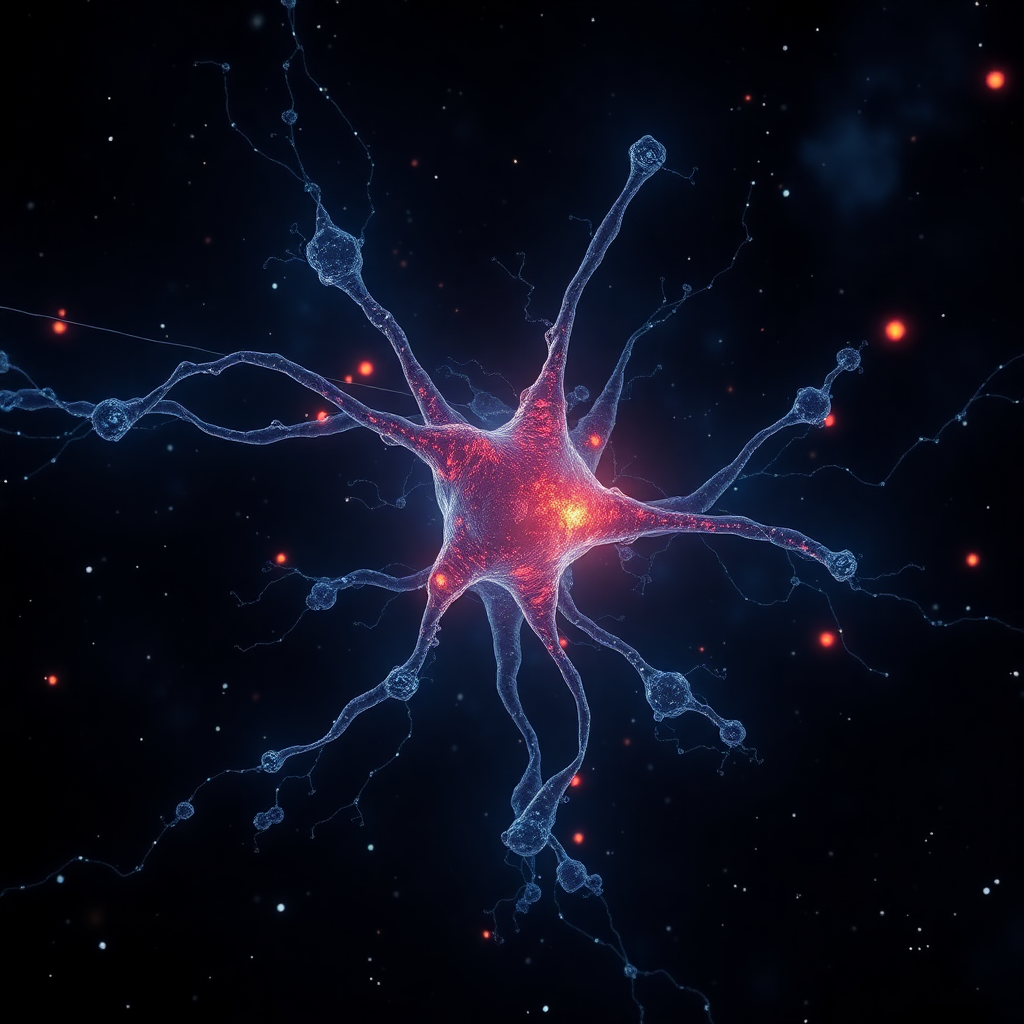
\includegraphics[width=0.8\textwidth]{images/astrocyte.png}

    \caption{Typical astrocyte.}
\end{figure}

The remarkable capacity of astrocytic networks to maintain coherent states while enabling dynamic responses becomes particularly evident in their role as regulators of neural excitability. Through careful modulation of extracellular ion concentrations and neurotransmitter levels, astrocytes help establish the precise conditions necessary for stable neural processing \cite{Araque2014}. This regulatory function extends beyond simple homeostasis to include active participation in information processing and state transitions.

Calcium signaling within astrocytic networks deserves particular attention \cite{Bazargani2016}. Unlike the rapid electrical signaling of neurons, astrocytes communicate through complex patterns of calcium waves that propagate across the syncytial network. These calcium signals can integrate information over longer temporal windows than neuronal activity, providing a mechanism for maintaining coherent states across extended periods. The patterns of calcium wave propagation reflect both local neural activity and broader network states, creating a sophisticated system for coordinating neural responses across multiple spatial and temporal scales.

The relationship between astrocytic networks and brain waves reveals another crucial aspect of conscious processing. Astrocytes help establish the conditions necessary for coherent oscillatory activity while modulating the spread of these oscillations through neural tissue \cite{Volterra2005}. Through regulation of extracellular ion concentrations and neurotransmitter dynamics, astrocytic networks can influence both the generation and propagation of brain waves. This interaction creates a feedback system where neuronal oscillations and astrocytic signaling work together to maintain stable patterns of conscious activity.

Gap junctions between astrocytes play an essential role in establishing the syncytial properties that enable coherent state maintenance \cite{Wallraff2006}. These direct cellular connections allow for rapid sharing of ions, metabolites, and small signaling molecules across extended spatial domains. The density and distribution of gap junctions can be dynamically regulated, providing a mechanism for modulating the extent and strength of network coupling based on current physiological demands.

The relationship between astrocytic networks and neural metabolism reveals sophisticated mechanisms for maintaining conscious states \cite{Parpura2012}. Through their extensive processes, astrocytes form specialized contacts with both blood vessels and synapses, creating a distributed system for matching energy supply to neural demand. This arrangement enables precise control over local metabolic conditions while maintaining broader patterns of energy distribution across neural tissue.

The integration of astrocytic networks with other brain systems demonstrates how biological organization can achieve both stability and flexibility through coordinated cellular interactions \cite{Khakh2015}. The ability of astrocytes to monitor and modulate neural activity while maintaining coherent energy states across extended spatial domains provides essential mechanisms for conscious processing. This sophisticated arrangement allows the brain to maintain stable conscious states while remaining adaptable to changing environmental demands.

Perhaps most significantly, astrocytic networks demonstrate how consciousness emerges not from neuronal activity alone but from the coordinated interaction of multiple cellular systems \cite{Nedergaard2003}. The continuous, field-like properties of astrocytic syncytia complement the discrete signaling of neurons, creating a hybrid system capable of supporting both rapid information processing and stable state maintenance. This integration of different cellular mechanisms proves essential for understanding how conscious states arise from biological organization.

The remarkable efficiency of astrocytic networks in managing ion homeostasis illustrates fundamental principles of conscious processing \cite{Bellot-Saez2017}. Through sophisticated regulation of extracellular potassium and calcium levels, these networks maintain the precise ionic conditions necessary for reliable neural signaling while preventing pathological states of over-excitation. This homeostatic function represents more than simple buffering - it creates the stable background conditions required for coherent conscious processing.

The study of astrocytic networks thus reveals fundamental principles about how biological systems achieve conscious processing \cite{Giaume2010}. Through their unique properties and extensive connectivity, astrocytes help create the conditions necessary for consciousness while providing mechanisms for maintaining coherent states across multiple spatial and temporal scales. This understanding proves essential for any complete theory of consciousness and suggests new approaches to both treating disorders of consciousness and developing artificial conscious-like systems.

The implications extend beyond neuroscience to fundamental questions about how biological systems maintain coherent states across multiple scales of organization \cite{Khakh2015}. The remarkable sophistication of gap junction networks demonstrates how evolution has refined cellular coupling mechanisms to support both stable conscious states and flexible adaptation to changing conditions. This deeper appreciation of biological connectivity proves essential for any complete theory of consciousness.

Moving beyond cellular networks, we must now examine how the extracellular matrix provides crucial structural and functional support for conscious processing. This complex network of proteins and molecules outside cells creates specialized microenvironments that shape both energy flows and information processing in neural tissue.

\section{The Extracellular Matrix}

The extracellular matrix serves as more than just structural scaffolding for neural tissue. It forms an active component of the brain's information processing and energy management systems \cite{Dityatev2010}. This complex network of proteins, proteoglycans, and other molecules fills the space between cells, creating a structured environment that shapes both ionic flows and molecular signaling while providing crucial support for maintaining coherent states.

The interaction between astrocytic networks and the ECM proves particularly important for maintaining energetic coherence across subsystems \cite{Song2018}. The ECM creates organized diffusion pathways that guide the movement of ions and neurotransmitters through the extracellular space, helping regulate local signaling environments while supporting broader patterns of communication across neural tissue. This structured diffusion plays an essential role in shaping both synaptic transmission and volume transmission between cells \cite{Sykova2008}.

The molecular composition and organization of the ECM varies systematically across brain regions, reflecting local functional requirements and computational demands \cite{Bandtlow2000}. These regional specializations create distinct microenvironments that support different aspects of neural processing. Through specific arrangements of matrix proteins and proteoglycans, the ECM helps establish and maintain the precise conditions necessary for different forms of neural computation and state maintenance \cite{Zimmermann2008}.

Perineuronal nets, specialized ECM structures that surround specific neuronal subtypes, demonstrate particularly sophisticated organization \cite{Wang2012}. These nets stabilize synaptic connections while regulating local ion concentrations, enabling sustained high-frequency firing patterns in certain neural populations. The precise molecular composition of perineuronal nets helps create stable microenvironments that support reliable neural signaling while allowing for controlled plasticity \cite{Kwok2011}.

The broader interstitial matrix that fills the space between cells serves multiple crucial functions in neural processing \cite{Ruoslahti1996}. Beyond providing structural support, this matrix guides molecular diffusion, supports volume transmission, and helps maintain proper spacing between cellular elements \cite{Nicholson1998}. The physical properties of the interstitial matrix influence both local signaling dynamics and broader patterns of communication across neural tissue.

The dynamic interaction between cellular components and the ECM creates a structured environment that supports both stability and adaptability in neural processing \cite{Dityatev2003}. Rather than serving as a static scaffold, the ECM actively participates in shaping neural activity through its influence on molecular diffusion, ion distribution, and cellular communication. This dynamic role proves essential for maintaining the coherent states necessary for conscious processing.

\begin{figure}[h]
    \centering
    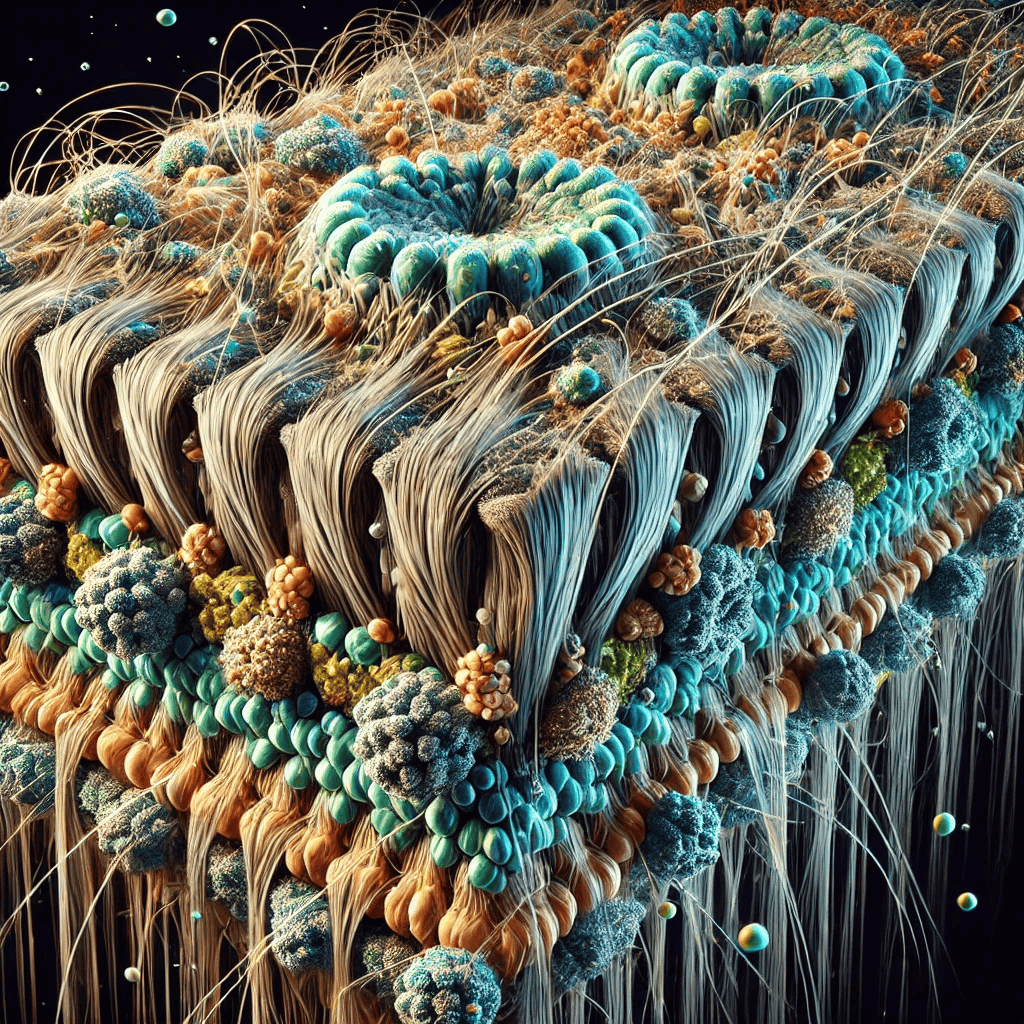
\includegraphics[width=0.8\textwidth]{ecm.png}

    \caption{The ECM guides ion flows and EM waves.}
\end{figure}

The ECM's influence on neural signaling extends beyond traditional synaptic transmission \cite{Vargova2014}. Through its capacity to bind and concentrate various signaling molecules, the matrix creates specialized signaling domains that shape both local and long-range communication. These domains help orchestrate complex patterns of neural activity while maintaining the stability necessary for coherent processing. The matrix's ability to sequester and release molecules in response to neural activity provides an additional layer of regulation in neural computation.

The relationship between the ECM and neural plasticity reveals sophisticated mechanisms for balancing stability and adaptability \cite{Dityatev2010}. While perineuronal nets help stabilize existing synaptic connections, local modifications of matrix composition can enable controlled reorganization of neural circuits \cite{Burnside2014}. This dynamic regulation of plasticity proves essential for learning and memory while maintaining the overall stability necessary for conscious processing.

Water and ion movement through the extracellular space depends critically on ECM organization \cite{Hrabetova2009}. The matrix creates structured pathways that guide fluid flow and ion diffusion, influencing both local signaling dynamics and broader patterns of neural activity. These pathways help maintain proper ionic balance while enabling efficient distribution of metabolites and removal of waste products. The resulting flow patterns support both local computation and global integration of neural activity.

The ECM's role in maintaining boundary conditions between different neural compartments deserves particular attention \cite{Barros2011}. Through specific molecular arrangements, the matrix helps establish and maintain distinct functional domains within neural tissue. These boundaries prove essential for proper circuit function while enabling controlled communication between different neural populations \cite{Frischknecht2012}. The precise organization of these boundary regions reflects evolutionary optimization for both isolation and integration of neural processing.

Matrix metalloproteinases and other ECM-modifying enzymes provide mechanisms for dynamic regulation of extracellular space properties \cite{Dityatev2003}. These enzymes can rapidly modify local matrix composition in response to neural activity, enabling adaptive changes in diffusion properties and signaling environments. This dynamic regulation allows neural circuits to adjust their processing capabilities while maintaining overall stability \cite{Song2018}.

The interaction between the ECM and glial cells represents another crucial aspect of neural organization \cite{Vargova2014}. Astrocytes actively participate in maintaining and modifying matrix composition, creating a feedback system that enables dynamic regulation of extracellular space properties. This interaction helps coordinate local changes in matrix structure with broader patterns of neural activity and metabolic demand.

The ECM's contribution to energetic coherence becomes particularly evident in its role in maintaining field effects across neural tissue \cite{Sykova2008}. The structured organization of matrix molecules influences the propagation of electromagnetic fields generated by neural activity, helping shape both local and global patterns of field interaction. This influence on field dynamics provides another mechanism through which the matrix contributes to conscious processing.

Understanding the ECM through ECC's framework reveals how seemingly passive structural elements can play active roles in consciousness \cite{Dityatev2010}. The matrix emerges not merely as a support system but as an essential component in maintaining the coherent energy states necessary for conscious experience. Its sophisticated molecular organization and dynamic properties enable both the stability required for reliable neural processing and the flexibility needed for adaptive responses \cite{Frischknecht2012}.

This deeper appreciation of the ECM's role suggests new approaches to both understanding and treating disorders of consciousness \cite{Burnside2014}. Matrix disruptions may contribute to various pathological conditions through their effects on neural signaling and energy coherence. Conversely, therapeutic interventions targeting matrix composition or organization might provide novel ways to influence conscious states and restore normal brain function.

The ECM's role extends beyond local circuit function to influence global brain dynamics \cite{Barros2011}. Through its effects on ion mobility, volume transmission, and field propagation, the matrix helps establish the conditions necessary for maintaining coherent states across multiple spatial scales. This multi-scale organization proves essential for understanding how consciousness emerges from coordinated neural activity \cite{Zimmermann2008}.

Having examined the biological components of neural tissue, we must now consider how to model the complex interactions within the neuropil that give rise to conscious states. This dense network of neural processes, glial cells, and extracellular matrix presents unique challenges for mathematical description and computational simulation.

\section{Neuropil Modeling}

The neuropil represents the brain's primary substrate for maintaining coherent conscious states, integrating cellular networks, ECM, and interstitial space into a unified functional domain. This dense meshwork of neural processes (including dendrites and their spines), glial elements, and extracellular structures creates an ideal medium for supporting organized energy flows and information integration \cite{Kasthuri2015}.

\begin{figure}[h]
    \centering
    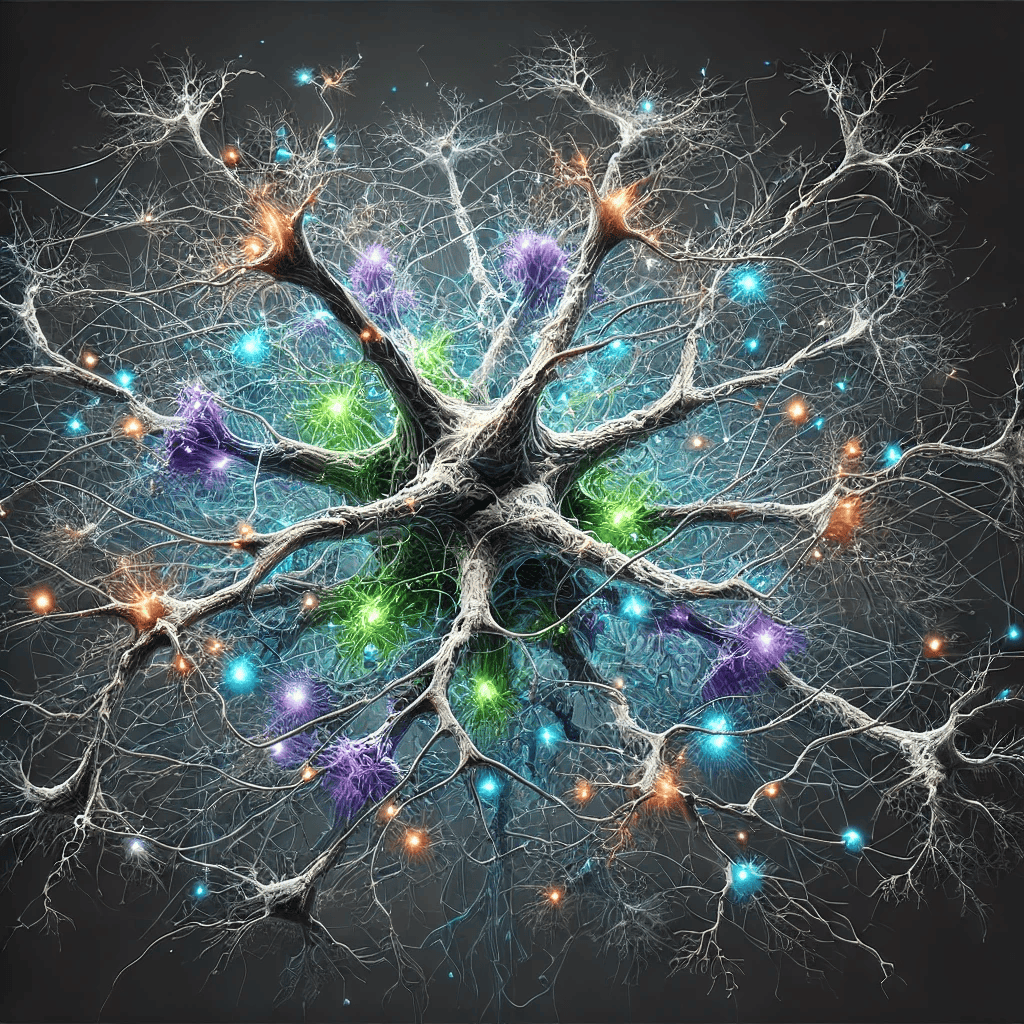
\includegraphics[width=0.8\textwidth]{neuropil.png}

    \caption{The neuropil is the most tangled layer of the cortical sheet}
\end{figure}

To model energetic coherence in the neuropil, we can employ the Jacobian of the stress-energy tensor with specific coupling terms that capture interactions between different components:

$\partial_\sigma T_{\mu\nu}(x) = \sum_i J_i(x) + \sum_{j,k} C_{jk}(x)$

\text{Where:}
\begin{itemize}
\item $T_{\mu\nu}$ represents the stress-energy tensor for the neuropil
\item $J_i$ captures local energy flows within specific components
\item $C_{jk}$ represents coupling terms between different elements
\item $x$ denotes position within the neuropil space
\end{itemize}

This organization creates the conditions necessary for sustained coherent states through the precise balance of energy flows across multiple scales \cite{Mishchenko2010}. When we examine the temporal evolution of these states, we can represent the dynamics using a modified form of the stress-energy tensor's Jacobian that incorporates both spatial and temporal derivatives:

$\partial_\sigma\partial_\tau T_{\mu\nu} = \sum_i \partial_\sigma J_i + \sum_{j,k} \partial_\tau C_{jk} + I_{\mu\nu}$

\text{Where:}
\begin{itemize}
\item $\partial_\sigma\partial_\tau$ represents the spatiotemporal evolution
\item $I_{\mu\nu}$ captures interface terms between adjacent regions
\end{itemize}

The interface terms are particularly important for understanding how coherent states propagate through the neuropil \cite{Doron2017}. These terms must satisfy certain continuity conditions:

$I_{\mu\nu}|_{\text{boundary}} = \text{continuous across regions}$

This constraint ensures smooth transitions between adjacent domains while maintaining global coherence. The neuropil's structure supports these transitions through specific biophysical mechanisms and architectural organization \cite{Korogod2015}.

1. Local Field Dynamics:

$\nabla \cdot \mathbf{E} = \frac{\rho}{\varepsilon}$

\text{Where:}
\begin{itemize}
\item $\mathbf{E}$ represents local field strength
\item $\rho$ captures charge density
\item $\varepsilon$ reflects local permittivity \cite{Savtchenko2014}
\end{itemize}

2. Wave Propagation:

$(\nabla^2 - \frac{1}{v^2}\frac{\partial^2}{\partial t^2})\psi = 0$

\text{Where:}
\begin{itemize}
\item $\psi$ represents the wave function
\item $v$ is the propagation velocity in the medium \cite{Arbib1998}
\end{itemize}

These equations describe how the neuropil supports both standing waves and propagating disturbances while maintaining coherent states. The solution space is constrained by the physical properties of the neuropil \cite{Peters1991}.

These constraints help ensure that energy flows remain within bounds that support conscious processing while allowing for dynamic responses to changing conditions \cite{Sorra2000}. The neuropil thus emerges as the critical substrate for implementing ECC's principles, providing both the physical structure and dynamic properties necessary for maintaining coherent conscious states.

\begin{figure}[h]
    \centering
    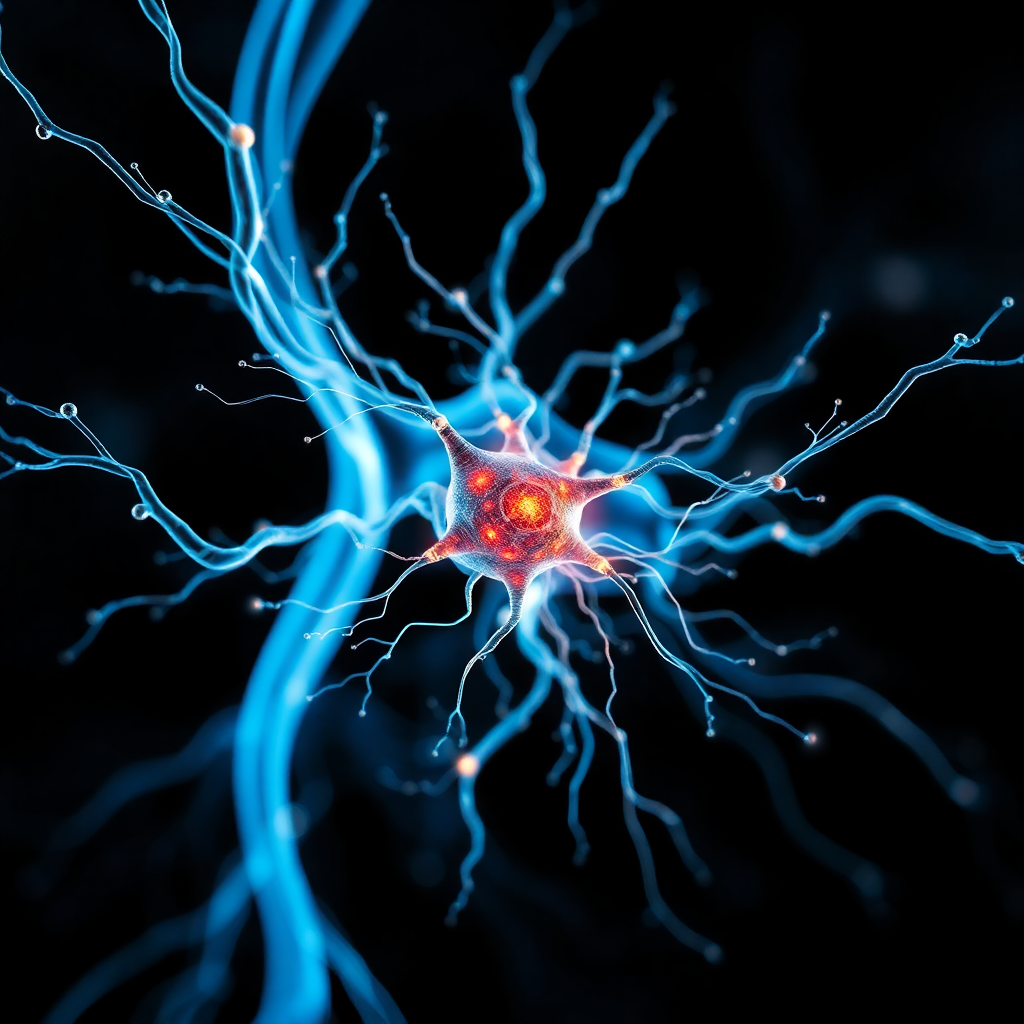
\includegraphics[width=0.8\textwidth]{images/neuropil2.png}

    \caption{Typical neuron of the neuropil.}
\end{figure}

The neuropil represents a critical domain for understanding how conscious states emerge from neural organization, as it provides the physical substrate where energetic coherence manifests at multiple scales \cite{Ventura1999}. This dense mesh of neural processes, glial extensions, and extracellular matrix creates the conditions necessary for maintaining coherent energy states while enabling dynamic information processing. Understanding how these components interact within the neuropil proves essential for any complete theory of consciousness.

The significance of neuropil organization extends beyond traditional connectionist approaches that focus primarily on synaptic connections between neurons \cite{Kasthuri2015}. Within this intricate space, multiple modes of communication operate simultaneously, including volume transmission, ephaptic coupling, and field effects that influence neural activity through non-synaptic mechanisms. These various forms of interaction create a rich landscape of possible states that supports both local processing and global integration of neural activity.

The physical properties of the neuropil prove particularly crucial for maintaining energetic coherence \cite{Korogod2015}. Its precise spatial organization enables the establishment of stable field patterns while allowing for rapid reconfiguration based on computational demands. The density and arrangement of cellular processes within the neuropil create conditions that support wave propagation while maintaining boundaries between different functional domains \cite{Arbib1998}. This balanced organization enables both segregation and integration of neural processing.

Astrocytic processes within the neuropil play an especially important role in maintaining coherent states \cite{Ventura1999}. Their extensive branching patterns and strategic positioning allow them to monitor and modulate synaptic activity while maintaining ion homeostasis across substantial volumes of tissue. The three-dimensional organization of astrocytic processes creates a continuous network that can coordinate energy distribution and maintain stable background conditions necessary for conscious processing.

The extracellular space within the neuropil, far from being a simple gap between cells, represents a highly structured environment that shapes both molecular diffusion and field effects \cite{Savtchenko2014}. The precise arrangement of extracellular matrix components influences how signals propagate through this space, affecting both local interactions and longer-range coordination. This structured environment proves essential for maintaining the specific patterns of energy flow that support conscious states.

The dynamic nature of neuropil organization deserves particular attention \cite{Sorra2000}. Rather than representing a static structure, the neuropil continuously adapts its properties in response to neural activity and metabolic demands. This adaptability enables sophisticated regulation of energy distribution and information processing while maintaining the stability necessary for coherent conscious experience. Understanding these dynamics proves crucial for developing accurate models of how consciousness emerges from neural activity.

Moreover, the neuropil's organization reflects evolutionary optimization for both information processing efficiency and energy management \cite{Peters1991}. The precise arrangement of cellular processes minimizes wiring length while maximizing computational capacity, creating conditions that support conscious processing while respecting metabolic constraints. This efficiency proves essential for maintaining coherent states across extended periods without excessive energy expenditure.

These considerations reveal why detailed modeling of neuropil organization and dynamics proves essential for understanding consciousness \cite{Mishchenko2010}. The emergence of coherent conscious states depends critically on the specific properties and interactions that occur within this complex domain. Any complete theory of consciousness must account for how the neuropil's structure enables both local processing and global integration while maintaining energetic efficiency.

The challenge of modeling neuropil dynamics reflects deeper questions about how consciousness emerges from biological organization \cite{Denk2004}. Traditional computational approaches, focused primarily on discrete neuronal interactions, fail to capture the continuous, field-like properties that arise from the neuropil's intricate structure. New mathematical frameworks must be developed that can represent both the discrete and continuous aspects of neural processing while accounting for the multiple scales of organization present in neural tissue.

The integration of various modeling approaches becomes particularly crucial when considering the neuropil's role in conscious processing \cite{Haehn2014}. Field theories must be combined with detailed cellular models, while accounting for the structured diffusion processes that occur in the extracellular space. These different perspectives must be unified through mathematical frameworks that can capture both the local dynamics of individual components and the emergent properties that arise from their collective interaction.

Perhaps most significantly, neuropil modeling reveals fundamental principles about how biological systems achieve conscious processing \cite{Helmstaedter2013}. The sophisticated organization of the neuropil, with its multiple overlapping domains of interaction and regulation, demonstrates how complex conscious states can emerge from physical processes while maintaining both stability and adaptability. This understanding proves essential for both theoretical developments in consciousness studies and practical applications in treating neurological disorders.

The implications extend beyond neuroscience to influence our broader understanding of consciousness itself \cite{White1986}. The neuropil's organization suggests that consciousness requires specific forms of physical implementation that support both local processing and global integration through continuous field-like interactions. This perspective challenges purely computational approaches to consciousness while suggesting new directions for developing artificial systems that might support conscious-like processing.

\section{Brodmann Areas}

The functional organization of the cortex into distinct Brodmann areas reflects a deeper principle of regional specialization that extends beyond cytoarchitecture to the molecular level. Each Brodmann area possesses a unique transcriptomic profile - a specific pattern of gene expression that shapes its information processing capabilities and energy management strategies \cite{Amunts2015}. These molecular signatures help explain how different regions maintain distinct functional properties while participating in the broader field of conscious experience.

Unlike the traditional view of Brodmann areas as purely structural divisions, modern neuroscience reveals them as domains of specialized molecular organization \cite{Amunts2007}. Brodmann areas represent distinct regions of the cerebral cortex, first mapped by neuroanatomist Korbinian Brodmann in the early 20th century based on their unique cytoarchitectural organization \cite{Brodmann1909}. These areas differ in the thickness of cortical layers, density of neurons, types of cells present, and patterns of connectivity. Originally identified through careful microscopic examination of cell structure and arrangement, these regions have since been shown to correspond closely with functional specialization in the brain \cite{Eickhoff2018}.

Each Brodmann area exhibits characteristic properties that reflect its role in processing specific types of information. For example, primary visual cortex (Brodmann area 17) shows a prominent layer 4 that receives direct thalamic input, while motor cortex (Brodmann area 4) is characterized by large pyramidal neurons in layer 5 that project to the spinal cord \cite{Zilles2010}. These structural differences support each region's specialized function while maintaining the capacity to integrate into broader conscious processes.

The functional organization of the cortex into distinct regions, mapped through careful cytoarchitectural analysis, takes on profound new significance when examined through the framework of energetically coherent computation. Far from being merely anatomical subdivisions, these areas represent domains of specialized molecular organization that enable distinct patterns of energetic coherence while maintaining integration with broader conscious processes \cite{Glasser2016}.

Unlike the traditional view of Brodmann areas as purely structural divisions, modern neuroscience reveals them as domains of sophisticated molecular organization \cite{Hawrylycz2012}. Each area maintains unique transcriptomic profiles that shape its capacity for information processing and energy management. These molecular signatures help explain how different regions maintain distinct functional properties while participating in the broader field of conscious experience.

The cellular architecture of each Brodmann area reflects evolutionary optimization for specific forms of information processing \cite{Palomero-Gallagher2019}. Areas devoted to sensory processing, such as primary visual cortex, demonstrate precisely organized cellular arrangements that support rapid, parallel processing of sensory inputs. In contrast, association areas maintain more flexible architectures that enable complex integration of information from multiple sources. These structural differences support each region's specialized function while maintaining the capacity for integration into broader conscious processes.

\begin{figure}[h]
    \centering
    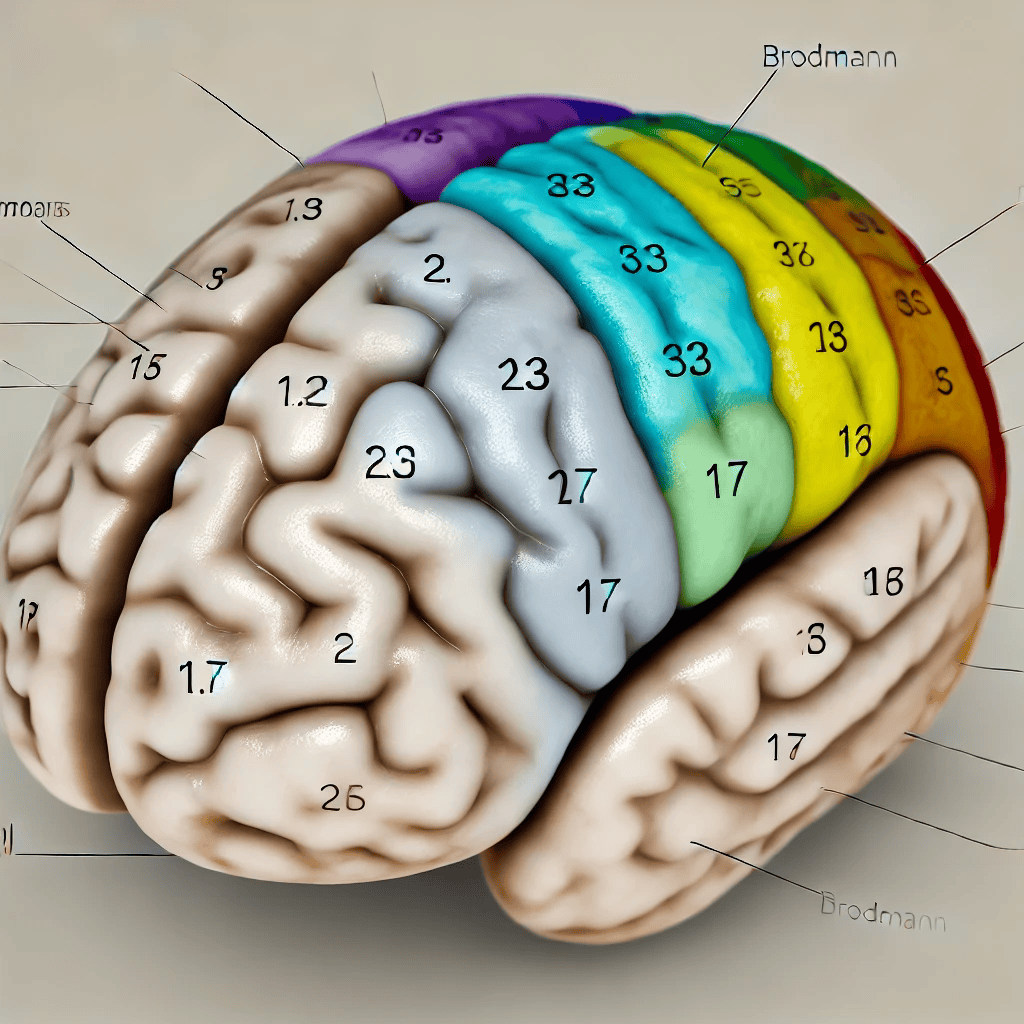
\includegraphics[width=0.8\textwidth]{brodmann.png}

    \caption{Brodmann areas align with great variation in transcriptomic profiles}
\end{figure}

The relationship between cellular organization and energetic coherence becomes particularly evident when examining how different Brodmann areas process information \cite{Passingham2002}. Primary sensory areas maintain tightly organized columns that enable precise mapping of sensory inputs while supporting stable patterns of energetic coherence. Association areas demonstrate more distributed patterns of organization that allow for flexible integration of information while maintaining coherent energy states across larger spatial domains.

Transcriptomic analysis reveals how each Brodmann area expresses distinct combinations of ion channels, receptors, and metabolic enzymes that shape its functional properties \cite{Lake2018}. These molecular profiles determine not just the computational capabilities of each region but also its capacity for maintaining specific patterns of energetic coherence. The resulting specialization enables sophisticated processing of different types of information while supporting integration into unified conscious experiences.

The patterns of connectivity between Brodmann areas reflect both computational requirements and energetic constraints \cite{VanEssen2012}. Long-range connections between regions must balance the need for efficient information transfer against the metabolic costs of maintaining extended axonal processes. This optimization creates networks that can support complex conscious processing while respecting fundamental energetic limitations.

The hierarchical organization of Brodmann areas reveals sophisticated principles of information processing and energy management \cite{Amunts2015}. Primary sensory areas maintain relatively rigid patterns of coherence that enable faithful representation of sensory inputs, while higher association areas demonstrate more flexible organizations that support abstract thought and complex integration. This hierarchy reflects not just computational specialization but different strategies for maintaining energetic coherence across varying temporal and spatial scales.

Understanding how Brodmann areas maintain distinct functional properties while enabling unified conscious experience represents a crucial challenge for consciousness research \cite{Scholtens2014}. The solution appears to lie in how each area achieves its specialized processing through unique patterns of energetic coherence that remain compatible with broader integration. This balance between specialization and integration emerges from the precise molecular and cellular organization of each region.

Building on the pioneering work of early neuroanatomists \cite{Vogt1919}, modern research has revealed increasingly sophisticated understanding of how regional specialization supports conscious processing. The precise laminar organization and cell-type distributions within each Brodmann area create the conditions necessary for maintaining specific patterns of energetic coherence while enabling integration into broader conscious states.

Perhaps most significantly, the study of Brodmann areas through ECC's framework suggests new approaches to understanding both normal conscious processing and pathological conditions \cite{Amunts2015}. Disorders affecting specific Brodmann areas may disrupt consciousness not just through loss of particular functions but through perturbation of broader patterns of energetic coherence. This perspective suggests novel therapeutic approaches targeting the restoration of normal energy dynamics rather than focusing solely on specific cellular pathologies.

The implications extend beyond clinical applications to fundamental questions about the nature of conscious experience \cite{Palomero-Gallagher2019}. The precise organization of Brodmann areas demonstrates how biological systems can achieve both specialized processing and global integration through sophisticated management of energetic coherence. This understanding proves essential for any complete theory of consciousness and suggests new directions for developing artificial systems capable of supporting conscious-like processing.

Recent advances in mapping brain organization have revealed increasingly complex patterns of regional specialization that extend beyond classical Brodmann parcellation \cite{Hawrylycz2012}. These findings suggest that the fundamental principles of regional organization - the careful balance between specialization and integration, the maintenance of specific energy dynamics, and the creation of stable processing domains - operate across multiple spatial scales.

The study of Brodmann areas thus reveals fundamental principles about how conscious processing emerges from neural organization \cite{Eickhoff2018}. Rather than representing arbitrary subdivisions, these regions reflect deep organizational principles that enable sophisticated information processing while maintaining the specific patterns of energetic coherence necessary for conscious experience. Understanding these principles proves crucial for both theoretical advances in consciousness studies and practical applications in treating neurological disorders.

Building on our understanding of regional specialization in the cortex, we must now examine how specific patterns of gene expression shape the capacity for conscious processing across different brain regions. These transcriptomic profiles create what ECC terms the "rich alphabet" of possible neural states, enabling sophisticated information processing while maintaining energetic coherence \cite{Lake2018}.

\section{Transcriptomic Profiles}

The molecular foundation of conscious processing emerges through distinct patterns of gene expression across neural tissues. These transcriptomic profiles create the fundamental basis for how different brain regions process information and maintain energetic coherence \cite{Tasic2018}. Unlike traditional approaches that focus primarily on neural connectivity or firing patterns, understanding consciousness through transcriptomic organization reveals how molecular diversity enables the rich repertoire of states necessary for conscious experience.

Each brain region maintains unique combinations of expressed genes that shape its functional capabilities through the production of specific ion channels, receptors, and regulatory proteins \cite{Bakken2021}. This molecular diversity proves essential for consciousness, as it enables neural tissues to support sophisticated information processing while maintaining stable patterns of energetic coherence. The resulting "rich alphabet" of possible neural states far exceeds what could be achieved through simple binary or digital encoding systems given the temporal, spatial and physical constraints under which the system operates. \footnote{Although any representation can be reduced to binary encoding, larger alphabets may have more expressive power. This can be beneficial under situations with resource constraints. In other words, abstractions matter.}

Within local circuits, transcriptomic diversity enables neurons to maintain distinct functional roles while participating in broader patterns of coherent activity \cite{Lake2016}. Different cell types express specific combinations of ion channels and receptors that determine their firing properties and response characteristics. This molecular specialization creates the conditions necessary for sophisticated information processing while ensuring that neural activity remains energetically efficient and properly regulated.

The relationship between transcriptomic profiles and astrocytic function deserves particular attention \cite{Zhang2010}. Astrocytes in different brain regions express distinct combinations of proteins that shape their capacity for maintaining ion homeostasis, regulating neurotransmitter levels, and coordinating metabolic support. These regional variations in astrocytic molecular properties prove crucial for maintaining the specific patterns of energetic coherence required for different aspects of conscious processing.

Gap junction proteins, crucial for establishing direct cellular coupling, show systematic variations in their expression across brain regions \cite{Yuste2020}. These differences in gap junction composition and density influence how effectively different areas can maintain coherent states through direct cellular communication. The resulting patterns of electrical and metabolic coupling help establish domains of coordinated activity that support conscious processing while maintaining energetic efficiency.

The dynamic regulation of gene expression in response to neural activity creates another crucial layer of control in conscious processing \cite{Fishell2020}. Transcriptomic profiles can shift in response to changing computational demands, enabling neural tissues to adapt their processing capabilities while maintaining overall stability. This molecular flexibility proves essential for supporting the dynamic nature of conscious experience while preserving coherent organization.

The relationship between transcriptomic profiles and metabolic regulation reveals sophisticated mechanisms for maintaining conscious states \cite{Macosko2015}. Different brain regions express specific combinations of metabolic enzymes and transporters that optimize their energy utilization for particular computational tasks. This specialized metabolic machinery enables regions to maintain stable patterns of energetic coherence while performing their distinct functional roles in conscious processing.

Regional variations in neurotransmitter receptor expression demonstrate how transcriptomic diversity shapes information processing across the brain \cite{Saunders2018}. Each area maintains specific combinations of receptor subtypes that determine its sensitivity to different neurotransmitters and neuromodulators. These molecular differences enable regions to process information in distinct ways while remaining integrated into broader patterns of conscious activity. The precise tuning of receptor expression helps establish the balance between excitation and inhibition necessary for maintaining coherent states.

The expression of membrane proteins that regulate ion flow proves particularly crucial for conscious processing \cite{Zeisel2018}. Different regions maintain distinct combinations of ion channels and transporters that shape their electrical properties and energy requirements. These molecular variations enable regions to support different patterns of neural activity while maintaining the stability necessary for conscious integration.

The role of transcription factors in regulating gene expression adds another layer of sophistication to conscious processing \cite{Nowakowski2017}. These regulatory proteins can rapidly modify which genes are expressed in response to changing neural activity or metabolic demands. This dynamic regulation enables neural tissues to adjust their molecular properties while maintaining overall coherence. The complex networks of transcriptional control help ensure that cellular adaptations remain coordinated across multiple scales of organization.

The relationship between transcriptomic profiles and synaptic organization reveals how molecular diversity shapes neural connectivity \cite{Angulo2022}. Different regions express distinct combinations of proteins involved in synaptic formation, maintenance, and modification. These molecular variations enable regions to establish and maintain the specific patterns of connectivity necessary for their roles in conscious processing.

The spatial organization of gene expression patterns demonstrates remarkable precision in supporting regional specialization \cite{Zeng2017}. The resulting molecular architecture creates domains of specialized processing capability while maintaining the flexibility necessary for integration into broader conscious states.

The implications of transcriptomic diversity extend beyond individual regions to shape how the brain maintains unified conscious experience \cite{Tasic2018}. The precise molecular complementarity between connected regions enables efficient communication while maintaining distinct processing capabilities. This balance between specialization and integration emerges from evolutionary optimization of gene expression patterns across neural networks, with different cell types showing remarkable consistency in their molecular signatures across individuals while maintaining clear regional distinctions.

Perhaps most significantly, transcriptomic profiles reveal fundamental principles about how biological systems achieve conscious processing \cite{Macosko2015}. The sophisticated organization of gene expression across brain regions demonstrates how molecular diversity enables complex information processing while maintaining energetic efficiency. The high-throughput analysis of individual cells has revealed unprecedented detail about the molecular basis of neural function and regional specialization.

Recent advances in single-cell RNA sequencing have provided remarkable insights into the diversity and specialization of neural populations \cite{Lake2016}. These techniques reveal how different cell types maintain distinct molecular profiles that shape their contribution to neural processing. The resulting molecular architecture creates what might be termed a "neural periodic table" - a systematic organization of cellular elements that together enable conscious processing.

The study of transcriptomic profiles through ECC's framework reveals consciousness as emerging not just from neural activity patterns but from precisely organized molecular systems \cite{Zeng2017}. This deeper appreciation of the molecular basis of consciousness opens new avenues for research while suggesting novel therapeutic approaches based on restoring normal patterns of gene expression and energy management.

Moving from broad patterns of gene expression to specific molecular interactions, we must now examine how cellular mechanisms implement the principles of energetically coherent computation. These mechanisms, operating across multiple scales from protein complexes to cellular assemblies, create the biological foundation for conscious processing through sophisticated management of energy flows and information integration.

\section{Molecular and Cellular Mechanisms}

The implementation of these specialized functions depends fundamentally on specific molecular and cellular mechanisms that link gene expression to energy dynamics. These mechanisms operate across multiple scales, from individual protein complexes to cellular assemblies, creating the biological foundation through which conscious processing emerges \cite{Baluska2016}. Far from simple molecular interactions, these mechanisms demonstrate remarkable sophistication in coordinating energy flows while maintaining information coherence across neural systems.

Membrane protein complexes serve as primary sites where electrical activity couples to cellular signaling \cite{Barker2018}. Rather than functioning as isolated units, these proteins form organized functional assemblies that enable precise control over neural signaling. Ion channels and receptors cluster into sophisticated complexes that shape both local computation and broader patterns of network activity. The resulting molecular architecture enables neural tissues to maintain stable processing while remaining responsive to changing conditions.

Second messenger systems demonstrate particular sophistication in coordinating cellular responses to neural activity \cite{Bashir2019}. Through calcium signaling cascades and cyclic nucleotide pathways, cells can integrate multiple inputs while maintaining coherent patterns of response. These molecular networks enable precise regulation of cellular function across multiple timescales, from rapid signaling events to longer-term adaptations. The resulting integration of signaling pathways proves essential for maintaining conscious states through sophisticated management of cellular activity.

The cytoskeletal system extends beyond mere structural support to play active roles in information processing and energy management \cite{Devor2016}. Dynamic structural proteins enable rapid reorganization of cellular architecture in response to neural activity, while motor proteins coordinate the movement of cellular components. This molecular machinery proves essential for maintaining the physical organization necessary for conscious processing while enabling adaptive responses to changing conditions. The continuous remodeling of cellular structure through cytoskeletal dynamics helps establish the conditions required for coherent neural activity.

The relationship between molecular mechanisms and cellular energetics reveals sophisticated principles of energy management in conscious systems \cite{Sengupta2014}. From mitochondrial function to ion gradient maintenance, cells employ multiple coordinated systems to match energy production to computational demands. These mechanisms operate through precise molecular interactions that enable efficient energy utilization while maintaining stable neural function. The resulting balance between energy availability and consumption proves crucial for sustaining conscious processing.

The integration of molecular mechanisms across different cellular compartments reveals another layer of sophistication in conscious processing \cite{Jonas2017}. Distinct sets of proteins operate in dendrites, axons, and synaptic terminals, enabling these compartments to perform specialized functions while maintaining coordinated activity. This subcellular specialization proves essential for establishing the complex patterns of information flow that support conscious experience.

The molecular basis of synaptic transmission demonstrates particular complexity in its organization and regulation \cite{Sudhof2018}. Beyond neurotransmitter release and reception, synapses employ sophisticated molecular machinery for maintaining precise timing relationships and controlling signal strength. Multiple protein complexes work together to coordinate vesicle cycling, receptor trafficking, and structural modification. This molecular coordination enables synapses to maintain reliable transmission while adapting to changing neural demands.

Protein phosphorylation networks create another crucial layer of cellular regulation in conscious processing \cite{Lane2018}. These molecular switches enable rapid modification of protein function in response to neural activity, creating dynamic patterns of cellular response that can be precisely controlled. Through coordinated action of kinases and phosphatases, cells maintain sophisticated control over their functional properties while preserving overall stability. The resulting molecular dynamics enable neural tissues to support complex information processing while maintaining coherent organization.

The regulation of membrane excitability through ion channel modulation reveals further complexity in cellular control mechanisms \cite{Marder2012}. Cells employ multiple molecular systems for adjusting their electrical properties in response to local conditions and broader network activity. These adaptive mechanisms operate through precise molecular interactions that enable neurons to maintain appropriate firing patterns while participating in larger-scale neural dynamics. The sophisticated regulation of cellular excitability proves essential for supporting conscious processing while preventing pathological activity.

Cellular calcium dynamics demonstrate remarkable sophistication in coordinating neural responses across multiple temporal and spatial scales \cite{Reese2016}. Through precisely organized molecular machinery, cells maintain complex patterns of calcium signaling that integrate multiple inputs and coordinate various cellular processes. These calcium dynamics enable neurons to perform complex computations while maintaining stable functional states. The resulting molecular coordination helps establish the conditions necessary for coherent conscious processing.

The molecular mechanisms underlying neural plasticity reveal sophisticated systems for modifying cellular properties while maintaining functional stability \cite{Takeuchi2014}. Through coordinated regulation of receptor trafficking, synaptic structure, and gene expression, cells can adapt their processing capabilities in response to experience. These molecular changes enable neural circuits to encode new information while preserving essential functional characteristics. The precise balance between stability and plasticity proves crucial for supporting conscious processing while enabling learning and memory.

The integration of these various molecular mechanisms creates a remarkably sophisticated system for information processing and energy management \cite{Wang2020}. Through careful coordination of multiple signaling pathways and regulatory systems, cells achieve both the stability necessary for reliable function and the flexibility required for adaptive response.

Perhaps most significantly, the study of molecular and cellular mechanisms through ECC's framework reveals how consciousness emerges from coordinated interactions across multiple scales of biological organization \cite{Sudhof2018}. From protein complexes to cellular assemblies, sophisticated molecular systems work together to create the conditions necessary for conscious processing. This understanding suggests new approaches to both investigating consciousness and developing therapeutic interventions for neurological disorders.

The temporal dynamics of molecular regulation demonstrate remarkable precision in maintaining coherent neural states \cite{Namburi2016}. Through carefully orchestrated sequences of protein modifications and cellular responses, neural circuits can adjust their processing capabilities while preserving essential functional relationships. This sophisticated timing enables the brain to maintain stable conscious states while adapting to changing environmental demands.

The relationship between molecular mechanisms and network function reveals fundamental principles about neural organization \cite{Lisman2018}. Rather than operating in isolation, cellular processes are precisely coordinated to support both local computation and broader patterns of network activity. This multi-scale integration proves essential for understanding how conscious processing emerges from biological mechanisms.

The implications extend beyond neuroscience to fundamental questions about how biological systems achieve conscious processing \cite{Yu2018}. The remarkable sophistication of molecular and cellular mechanisms demonstrates how evolution has refined these systems to support both stable conscious states and dynamic adaptation to changing conditions. This deeper appreciation of biological complexity proves essential for any complete theory of consciousness and suggests new directions for developing artificial systems capable of supporting conscious-like processing \cite{Zador2019}.

\section{Membrane Dynamics}

At the heart of cellular mechanisms lies the cell membrane, which serves as far more than a simple boundary between internal and external environments. This sophisticated interface plays a crucial role in implementing ECC's principles through the precise regulation of ion flows, protein organization, and local electric fields \cite{Andersen1992}. The cell membrane emerges not as a passive barrier but as an active participant in information processing and energy management, fundamentally shaping how neural systems maintain coherent conscious states.

The phospholipid bilayer structure creates a highly organized environment where proteins can be precisely arranged and regulated to support conscious processing \cite{Goni2014}. This molecular organization enables several crucial processes that extend beyond basic cellular containment. Through careful maintenance of ion gradients and electrochemical potentials, membranes establish the fundamental conditions necessary for neural signaling and information processing. The resulting electrical properties enable neurons to maintain stable resting states while remaining capable of rapid, coordinated responses to incoming signals.

Lateral organization within the membrane reveals another layer of sophistication in cellular processing \cite{Garcia-Parajo2014}. Specialized membrane domains create distinct regions where specific proteins cluster together, enabling precise control over cellular signaling and energy management. These domains prove essential for coordinating the complex molecular interactions that underlie neural computation. Through dynamic reorganization of membrane components, cells can modify their processing capabilities while maintaining overall stability.

The membrane's role in generating and maintaining electric fields takes on particular significance for conscious processing \cite{Bezanilla2002}. Local variations in membrane potential create sophisticated patterns of field effects that influence both protein function and cellular signaling. These field effects extend beyond individual cells to shape network dynamics through ephaptic coupling and other non-synaptic mechanisms. The resulting electromagnetic properties of neural membranes contribute fundamentally to the establishment and maintenance of coherent conscious states.

The dynamic interplay between membrane structure and protein function demonstrates remarkable sophistication in neural information processing \cite{Kusumi2012}. Membrane proteins respond to changes in local electrical fields and mechanical forces, creating feedback loops that enable precise regulation of cellular activity. This intimate coupling between membrane properties and protein function enables neural systems to maintain stable processing capabilities while adapting to changing conditions.

The relationship between membrane dynamics and energy management reveals sophisticated mechanisms for maintaining conscious states \cite{Yang2019}. Through precisely regulated ion pumps and transport proteins, membranes help establish and maintain the energy gradients necessary for neural signaling. These molecular systems operate continuously to preserve the specific electrical properties required for information processing while managing cellular energy consumption.

\begin{figure}[h]
    \centering
    \includegraphics[width=0.8\textwidth]{images/membrane.png}

    \caption{Membranes have phospholipid bilayer structure.}
\end{figure}

Membrane fluidity plays a crucial role in enabling dynamic responses to neural activity \cite{Lingwood2010}. The capacity for lipids and proteins to move laterally within the membrane creates opportunities for rapid reorganization of signaling complexes and regulatory systems. This molecular mobility enables cells to adjust their processing capabilities through precise changes in protein organization and interaction. The controlled fluidity of neural membranes thus provides a fundamental mechanism for adapting to changing computational demands while maintaining functional stability.

The interface between membranes and the cytoskeleton reveals another layer of cellular regulation in conscious processing \cite{Zimmerberg2006}. Membrane proteins interact with cytoskeletal elements to create structured domains that shape both cellular architecture and signaling properties. These interactions enable precise control over protein distribution and movement while providing mechanical stability to cellular structures. The resulting membrane-cytoskeleton coupling helps establish the organized cellular domains necessary for coherent neural activity.

Lipid composition demonstrates remarkable regional variation that reflects different requirements for neural processing \cite{Yang2019}. Different areas of the membrane maintain distinct combinations of lipid species that influence local properties such as fluidity, thickness, and protein organization. These molecular variations enable cells to establish specialized domains for particular aspects of neural computation while maintaining overall membrane integrity. The precise tuning of lipid composition proves crucial for supporting the diverse functions required for conscious processing.

The role of membrane dynamics in synaptic transmission extends far beyond simple neurotransmitter release \cite{Sudhof2013}. Presynaptic membranes undergo sophisticated reorganization during vesicle fusion and recycling, while postsynaptic membranes coordinate complex patterns of receptor trafficking and clustering. These dynamic processes enable synapses to maintain reliable transmission while adapting their properties based on neural activity. The resulting synaptic plasticity depends fundamentally on precise regulation of membrane organization and dynamics.

The integration of membrane dynamics with broader patterns of neural activity reveals fundamental principles about how conscious processing emerges from cellular mechanisms \cite{Choquet2013}. Membranes serve as sophisticated interfaces that enable cells to participate in coherent network activity while maintaining their specific processing capabilities. Through precise regulation of protein organization, ion flows, and electrical properties, membranes help establish the conditions necessary for consciousness while supporting dynamic adaptation to changing demands.

The coordination between membrane organization and energy metabolism demonstrates remarkable efficiency in neural processing \cite{Goni2014}. The precise arrangement of transport proteins and metabolic machinery enables cells to maintain the energy gradients necessary for signaling while minimizing metabolic costs. This optimization reflects evolutionary refinement of membrane organization for both computational capability and energetic efficiency.

\begin{figure}[h]
    \centering
    \includegraphics[width=0.8\textwidth]{membrane.png}

    \caption{The cell membrane is where the cell receives all external information. }
\end{figure}

Perhaps most significantly, membrane dynamics demonstrate how biological systems achieve sophisticated information processing through continuous physical processes rather than discrete computational steps \cite{Sachs2010}. The fluid nature of membrane organization, coupled with precise molecular regulation, enables neural systems to maintain stable conscious states while remaining responsive to changing conditions. This understanding proves essential for explaining how consciousness emerges from biological organization rather than abstract computation.

The implications extend beyond neuroscience to fundamental questions about the nature of conscious processing \cite{Zimmerberg2006}. The remarkable sophistication of membrane dynamics suggests that consciousness requires specific forms of physical implementation that support both stability and adaptability through continuous regulation of cellular properties. This perspective challenges purely computational approaches to consciousness while suggesting new directions for developing artificial systems capable of supporting conscious-like processing.

Moving beyond membrane dynamics, we must now examine how neurotransmitter and neuromodulatory systems influence conscious processing through broad-scale regulation of neural activity \cite{Choquet2013}. These sophisticated molecular signals reshape network properties and energy dynamics across multiple spatial and temporal scales, fundamentally altering how neural circuits maintain coherent conscious states.

\section{Neurotransmitters and Neuromodulators}

The chemical basis of neural signaling reveals sophisticated mechanisms for maintaining coherent conscious states through the coordinated action of neurotransmitters and neuromodulators. While fast synaptic transmission through classical neurotransmitters enables precise information processing, neuromodulatory systems reshape network properties across broader spatial and temporal scales \cite{Nadim2014}. This dual system of chemical signaling proves essential for consciousness, enabling both rapid computation and sustained regulation of neural states.

Classical neurotransmitters like glutamate and GABA establish the fundamental patterns of excitation and inhibition necessary for neural processing \cite{Froemke2015}. Through precisely controlled release at synaptic sites, these molecules enable rapid communication between neurons while maintaining careful balance in network activity. The sophisticated regulation of synaptic transmission through multiple receptor systems allows neural circuits to perform complex computations while avoiding pathological states of over- or under-activation.

The broader influence of neuromodulatory systems fundamentally reshapes how neural circuits maintain coherent states \cite{Marder2012}. Molecules like dopamine, serotonin, norepinephrine, and acetylcholine act through volume transmission to influence large populations of neurons simultaneously. These signals alter the basic operating parameters of neural circuits, changing how cells respond to inputs and modifying patterns of synaptic plasticity. The resulting modulation enables neural networks to adapt their processing capabilities while maintaining overall stability.

The spatial organization of these signaling systems demonstrates remarkable sophistication in regulating conscious processing \cite{Bargmann2012}. While classical neurotransmitters operate primarily at discrete synaptic sites, neuromodulators diffuse through the extracellular space to influence broader domains of neural tissue. This architectural difference enables coordinated regulation of neural properties across distributed circuits while preserving the specificity of local information processing. The resulting balance between precise transmission and broad modulation proves essential for conscious processing.

The temporal dynamics of chemical signaling add another layer of control to conscious processing \cite{Palacios-Filardo2019}. Classical neurotransmission operates on millisecond timescales, enabling rapid information processing through precise timing of neural activity. In contrast, neuromodulatory effects can persist for seconds to hours, creating sustained changes in how circuits process information. This temporal diversity enables neural systems to maintain stable conscious states while remaining capable of rapid responses to changing conditions.

The interaction between different chemical signaling systems reveals sophisticated principles of neural regulation \cite{Dayan2012}. Neuromodulators influence how classical neurotransmitters function, altering release probability, receptor sensitivity, and patterns of synaptic plasticity. These interactions enable complex forms of neural computation that can be dynamically adjusted based on behavioral state and cognitive demands.

The role of peptide neurotransmitters adds further complexity to neural signaling \cite{Nadim2014}. These larger molecules act through distinct mechanisms from classical neurotransmitters, often producing slower but longer-lasting effects on neural function. Neuropeptides can fundamentally alter how circuits process information, creating sustained changes in network properties that influence conscious processing. Their sophisticated regulation and diverse effects demonstrate how chemical signaling extends far beyond simple excitation or inhibition.

The relationship between chemical signaling and energy metabolism reveals another crucial aspect of conscious processing \cite{Marder2012}. Neuromodulatory systems influence how neural circuits utilize energy, adjusting metabolic processes to match computational demands. This coordination between signaling and metabolism enables neural systems to maintain efficient processing while avoiding energetic depletion. The resulting balance proves essential for sustaining conscious states across extended periods.

Different brain regions show distinct patterns of sensitivity to neuromodulatory signals \cite{Parr2017}. These regional variations emerge from specific combinations of receptor expression and local circuit properties that shape how areas respond to modulatory inputs. Such specialization enables sophisticated regulation of neural function while maintaining distinct processing capabilities across different brain regions. The resulting modulatory architecture helps establish the complex patterns of neural activity that support conscious experience.

The regulation of synaptic plasticity through chemical signaling demonstrates particular sophistication \cite{Froemke2015}. Neuromodulators determine when and how synaptic connections change in response to neural activity, shaping both rapid adjustments and longer-term modifications of circuit function. This control over plasticity enables neural networks to encode new information while maintaining stable processing capabilities. The precise regulation of synaptic modification proves crucial for supporting learning and memory within conscious systems.

The integration of neurotransmitter and neuromodulatory systems reveals fundamental principles about how biological systems achieve conscious processing \cite{Picciotto2012}. Rather than operating through simple binary signals, neural systems employ sophisticated chemical mechanisms that enable both precise computation and broad regulatory control. This dual system of fast transmission and sustained modulation creates the conditions necessary for maintaining coherent conscious states while enabling dynamic adaptation to changing demands.

The interplay between different neuromodulatory systems creates complex patterns of circuit regulation \cite{Cools2011}. Through careful coordination of multiple signaling pathways, neural circuits can achieve remarkable flexibility in their processing capabilities while maintaining overall stability. This sophisticated chemical orchestration proves essential for supporting the diverse computational requirements of conscious processing.

Perhaps most significantly, the study of chemical signaling through ECC's framework reveals how consciousness emerges from coordinated molecular interactions rather than abstract computation \cite{Marder2012}. The remarkable sophistication of neurotransmitter and neuromodulatory systems demonstrates how evolution has refined these mechanisms to support both stable conscious states and flexible adaptation to changing conditions. This understanding proves essential for explaining how biological systems achieve conscious processing while suggesting new approaches to treating disorders of consciousness.

The implications extend beyond neuroscience to fundamental questions about the nature of information processing in conscious systems \cite{Dayan2012}. The complex interplay between fast synaptic transmission and broader neuromodulation suggests that consciousness requires specific forms of chemical regulation that cannot be reduced to simple computational operations. This perspective challenges purely digital approaches to artificial consciousness while suggesting new directions for developing systems capable of supporting conscious-like processing.

Moving deeper into the molecular foundations of consciousness, we must now examine how proteins maintain and transition between multiple conformational states to support conscious processing. These molecular configurations represent more than simple switches - they create a rich landscape of possible states that enables sophisticated information processing while maintaining energetic coherence \cite{Nadim2014}.

\section{Protein States}

The dynamic behavior of membrane proteins, particularly their ability to adopt multiple conformational states, provides a crucial mechanism for implementing ECC's principles. These protein states represent more than simple on-off switches; they create a rich repertoire of possible configurations that can encode and process information while maintaining direct connection to physical energetics \cite{Balchin2016}. The sophisticated transitions between these states enable neural systems to achieve both stability and flexibility in conscious processing.

Ion channels demonstrate remarkable complexity in their conformational dynamics, maintaining multiple conductance states that respond to various cellular signals \cite{Henzler-Wildman2007}. Rather than operating as simple gates, these proteins transition through numerous functional configurations influenced by voltage, ligand binding, and mechanical forces. This diversity of possible states enables sophisticated regulation of neural activity while providing mechanisms for maintaining stable patterns of network function. The precise control of these conformational changes proves essential for supporting conscious processing.

Receptor proteins exhibit even greater sophistication in their state transitions, integrating multiple inputs through complex patterns of allosteric regulation \cite{Nussinov2013}. Individual receptors can adopt numerous configurations that shape both their binding properties and downstream signaling effects. These varied states enable cells to perform complex computations at the molecular level while maintaining energetic efficiency. The resulting molecular computation occurs through physical state changes rather than abstract symbol manipulation.

Structural proteins contribute to conscious processing through their own complex state dynamics \cite{Frauenfelder2009}. Rather than serving as static scaffolds, these proteins undergo continuous conformational changes that respond to and influence cellular activity. Their dynamic assembly states and force-sensitive configurations enable sophisticated regulation of cellular architecture while supporting stable neural function. This molecular flexibility proves crucial for maintaining the physical organization necessary for conscious processing.

The energetic aspects of protein states take on particular significance within ECC's framework \cite{Karplus2005}. Each conformational state represents a distinct energy minimum within a complex landscape of possible configurations. Transitions between states follow specific energetic pathways that enable reliable information processing while maintaining thermodynamic efficiency. The precise organization of these energy landscapes through evolution has created molecular systems capable of supporting conscious processing.

The coupling between protein states and cellular energy dynamics creates sophisticated systems for information processing grounded in physical transitions \cite{Zhou2008}. Rather than operating through abstract representations, neural computations emerge from actual changes in molecular configuration that remain directly connected to energy flows. This physical basis for information processing proves essential for understanding how conscious systems maintain coherent states while enabling dynamic responses to changing conditions.

\begin{figure}[h]
    \centering
    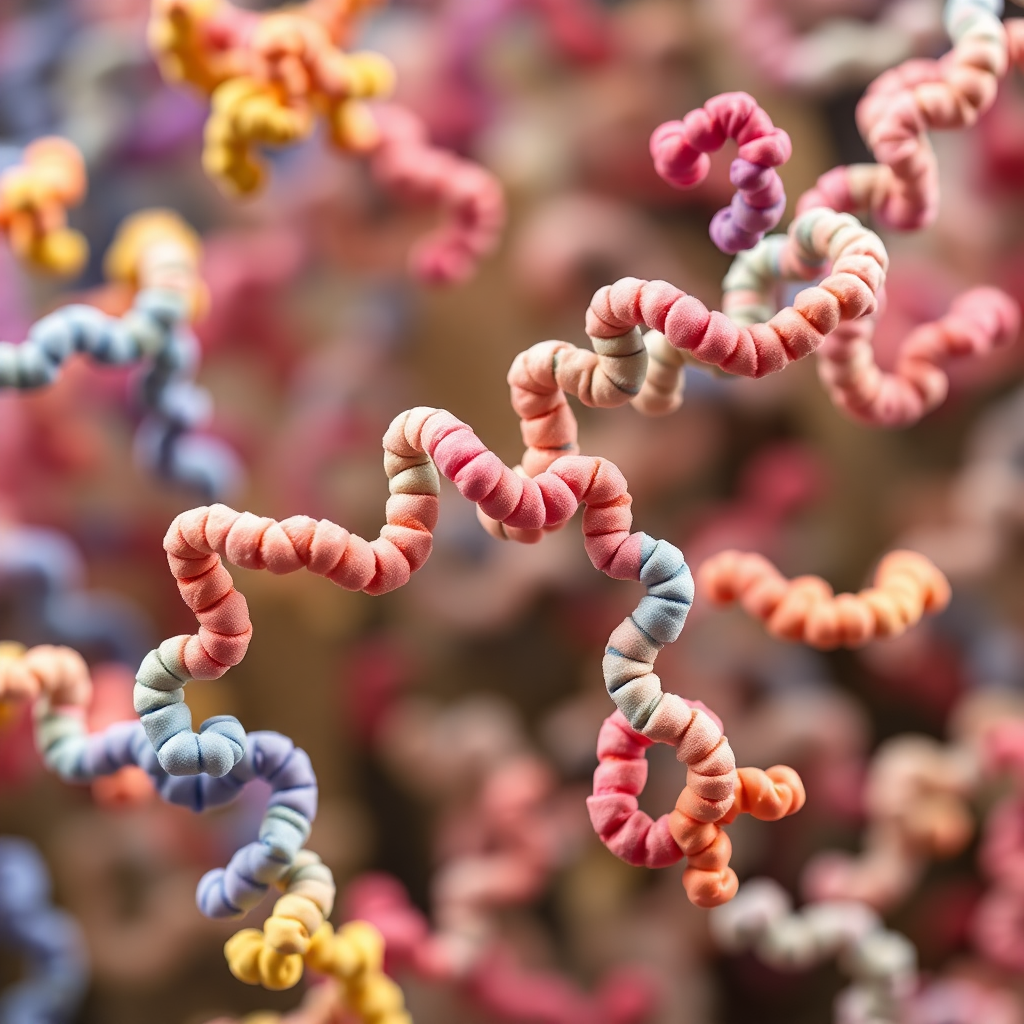
\includegraphics[width=0.8\textwidth]{images/protein.png}

    \caption{Depiction of a long strand of a protein.}
\end{figure}

Receptor oligomers reveal particularly complex patterns of state transitions in their molecular organization \cite{Lindorff-Larsen2016}. These protein assemblies can adopt various configurations depending on their molecular environment and activation state, creating rich possibilities for information encoding through physical states. The cooperative interactions between subunits enable sophisticated integration of multiple signals while maintaining stable functional properties. Their precise molecular architecture allows for both sensitivity to specific inputs and resistance to random fluctuations.

The stoichiometry of protein complexes plays a crucial role in determining their possible state transitions \cite{Brangwynne2015}. The precise ratios of different protein subunits within receptor complexes and ion channels shape both their functional properties and energy requirements. These molecular relationships establish specific constraints on how proteins can transition between states while maintaining stable function. The resulting balance between flexibility and stability proves essential for supporting conscious processing.

Post-translational modifications add another layer of control to protein state dynamics \cite{Wright2015}. Chemical modifications like phosphorylation can rapidly alter protein conformations, creating additional possibilities for information encoding through molecular states. These modifications enable cells to adjust protein function in response to ongoing activity while maintaining overall stability. The sophisticated regulation of protein states through chemical modification provides mechanisms for both rapid signaling and sustained changes in cellular properties.

The relationship between protein states and local electric fields demonstrates remarkable sophistication in neural information processing \cite{Tokuriki2009}. Membrane proteins respond to changes in electrical potential through precise conformational changes that alter their functional properties. These voltage-dependent state transitions enable rapid signaling while maintaining energetic efficiency. The resulting coupling between electrical activity and protein conformation creates fundamental mechanisms for neural computation through physical state changes.

The integration of protein states across multiple scales reveals fundamental principles about how biological systems achieve conscious processing \cite{Thirumalai2017}. From individual molecules to cellular assemblies, sophisticated state transitions enable complex information processing while maintaining direct connection to physical energy dynamics. This understanding suggests that consciousness emerges not from abstract computation but from precisely organized patterns of molecular state changes that support both stability and adaptability.

The crowded cellular environment introduces additional complexity to protein state dynamics \cite{Roh2017}. Molecular crowding effects influence both the stability of different conformational states and the kinetics of transitions between them. This physical constraint shapes how proteins function within the dense cellular milieu while providing additional mechanisms for regulating their behavior.

\begin{figure}[h]
    \centering
    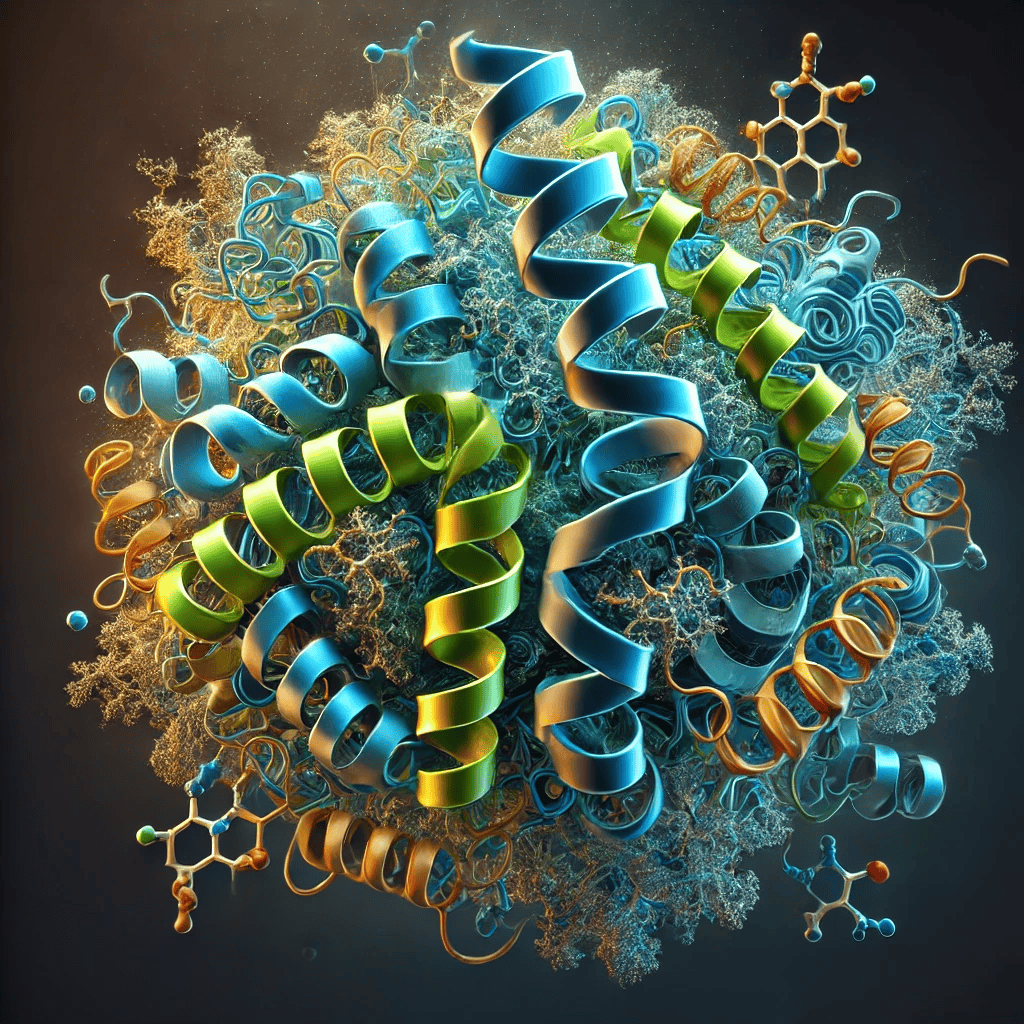
\includegraphics[width=0.8\textwidth]{proteins.png}

    \caption{Proteins can take on exotic conformations}
\end{figure}

Perhaps most significantly, the study of protein states through ECC's framework reveals how information processing can remain grounded in physical transitions while achieving remarkable computational sophistication \cite{Oldfield2014}. Rather than requiring abstraction into symbolic representation, neural computation occurs through actual changes in molecular configuration that maintain direct connection to energy flows. This perspective challenges purely computational approaches to consciousness while suggesting new directions for developing artificial systems capable of supporting conscious-like processing.

The implications extend beyond neuroscience to fundamental questions about the nature of information processing in biological systems \cite{Davis2018}. The remarkable sophistication of protein state dynamics demonstrates how evolution has refined molecular mechanisms to support both stable conscious states and flexible adaptation to changing conditions. This deeper appreciation of molecular complexity proves essential for any complete theory of consciousness and suggests new approaches to treating disorders of conscious processing.

The relationship between protein states and neural energetics reveals fundamental principles about biological computation \cite{Erickson2009}. The precise organization of conformational landscapes enables sophisticated information processing while maintaining direct connection to physical energy flows. This grounding in molecular dynamics helps explain how conscious systems achieve both stability and flexibility through carefully orchestrated patterns of state transitions \cite{Royer2006}.

Moving beyond individual proteins to examine direct cellular coupling, we must now consider how gap junctions enable coherent state maintenance across neural tissues. These specialized channels, composed of connexin proteins, create electrical synapses that allow for rapid, bidirectional communication between cells, proving essential for maintaining the coherent energy states necessary for conscious processing.

\section{Gap Junctions}

While individual protein states provide a basis for information encoding, gap junctions create direct cytoplasmic continuity between cells, enabling a fundamentally different form of information sharing and energy coupling. These specialized protein channels, composed of connexin proteins, form electrical synapses that allow for rapid, bidirectional communication between cells \cite{Giaume1996}. Unlike chemical synapses that rely on neurotransmitter release and receptor activation, gap junctions provide immediate electrical and metabolic coupling between connected cells.

The importance of gap junctions in neural processing extends far beyond simple electrical coupling. These channels enable the formation of functional syncytia - networks of coupled cells that can share states and coordinate their activities with minimal delay \cite{Bennett2004}. In neuronal networks, gap junctions prove particularly crucial for synchronizing populations of inhibitory interneurons, enabling precise temporal control over circuit activity. This rapid synchronization helps establish the coherent patterns of neural activity necessary for conscious processing.

Within glial networks, gap junctions take on even greater significance \cite{Dermietzel2013}. Astrocytes connected through these channels form extensive syncytial networks that can coordinate both metabolic support and information processing across substantial volumes of neural tissue. These networks enable sophisticated distribution of resources while maintaining stable background conditions for neural activity. The resulting patterns of cellular coupling provide essential mechanisms for supporting coherent conscious states.

The electrical properties of gap junctions demonstrate remarkable sophistication in their contribution to neural processing \cite{Connors2004}. These channels create low-resistance pathways between cells that enable rapid signal propagation while maintaining distinct functional domains. The voltage-dependent gating of gap junctions provides mechanisms for regulating cellular coupling based on local activity patterns. This dynamic regulation helps establish domains of coordinated activity that can maintain coherent states while adapting to changing conditions.

The molecular diversity of connexin proteins enables precise control over gap junction properties across different neural populations \cite{Willecke2002}. Various connexin subtypes create channels with distinct conductance properties and regulatory sensitivities, allowing for sophisticated modulation of cellular coupling. This molecular specialization enables neural tissues to maintain appropriate patterns of electrical and metabolic coupling while supporting diverse forms of information processing.

The regulation of gap junction coupling demonstrates sophisticated mechanisms for controlling cellular communication \cite{Nagy2018}. Conductance through these channels responds dynamically to various cellular signals, including voltage differences between cells, changes in pH and calcium levels, and modulation by phosphorylation states. This multilayered regulation enables precise control over cellular coupling while maintaining network stability.

The relationship between gap junctions and metabolic coordination reveals another crucial aspect of their function in conscious processing \cite{Hormuzdi2004}. These channels enable direct sharing of small molecules and metabolites between coupled cells, creating efficient pathways for distributing resources across neural tissues. This metabolic coupling helps maintain stable energy states while supporting dynamic patterns of neural activity. The coordination of cellular metabolism through gap junctions provides fundamental mechanisms for sustaining conscious processing.

Gap junctions play a particularly important role in establishing what might be termed coherence domains within neural tissue - regions where cells can maintain synchronized states through direct coupling \cite{Pannasch2013}. These domains emerge from the precise organization of gap junction connectivity, creating structured patterns of cellular communication that support conscious processing. The resulting network architecture enables both local coordination and broader patterns of coherent activity across neural populations.

The interaction between gap junctions and chemical synapses reveals sophisticated principles of neural organization \cite{Pereda2014}. Rather than operating independently, these different forms of cellular communication work together to create complex patterns of network activity. Gap junctions provide rapid synchronization and state sharing, while chemical synapses enable more nuanced control over information flow. This dual system of communication proves essential for maintaining coherent conscious states while enabling flexible neural computation.

The role of gap junctions in development and plasticity demonstrates their importance beyond immediate cellular coupling \cite{Nadarajah1996}. These channels influence how neural circuits form and modify their connectivity patterns, shaping both cellular differentiation and circuit refinement. The resulting patterns of gap junction connectivity reflect both genetic programming and activity-dependent modification. This developmental regulation helps establish the specific network architectures necessary for conscious processing.

The biophysical properties of gap junctions create unique opportunities for information processing \cite{Palacios-Prado2009}. The direct electrical coupling between cells enables forms of computation that would be impossible through chemical synapses alone. This specialized signaling capability proves particularly important for coordinating rapid responses across neural populations and maintaining coherent activity patterns.

The integration of gap junctional coupling with broader patterns of neural activity reveals fundamental principles about how conscious processing emerges from cellular interactions \cite{Nielsen2012}. Through their ability to create direct cellular coupling while maintaining dynamic regulation, gap junctions help establish the conditions necessary for consciousness. The resulting balance between rapid communication and controlled isolation enables neural systems to maintain coherent states while supporting complex information processing.

Perhaps most significantly, gap junctions demonstrate how biological systems achieve sophisticated coordination through physical mechanisms rather than abstract computation \cite{Bennett2004}. The direct sharing of electrical and metabolic states through these channels creates forms of cellular coupling that cannot be reduced to digital information processing. This understanding suggests new approaches to both studying consciousness and developing therapeutic interventions for neurological disorders.

The functional diversity of gap junction coupling across different neural populations reveals fundamental organizing principles of conscious processing \cite{Connors2004}. Different cell types and brain regions utilize distinct patterns of gap junction connectivity to achieve specific computational goals while maintaining broader network coherence. This architectural specialization demonstrates how biological systems can achieve both local specificity and global integration through direct cellular coupling.

The implications extend beyond neuroscience to fundamental questions about how biological systems maintain coherent states across multiple scales of organization \cite{Giaume1996}. The remarkable sophistication of gap junction networks demonstrates how evolution has refined cellular coupling mechanisms to support both stable conscious states and flexible adaptation to changing conditions. This deeper appreciation of biological connectivity proves essential for any complete theory of consciousness \cite{Hormuzdi2004}.

Moving beyond cellular networks, we must now examine how the cytoskeleton and its dynamic properties contribute to maintaining coherent conscious states. While previous theories have emphasized quantum effects in microtubules, the classical role of the cytoskeleton in organizing cellular energy dynamics and information processing provides crucial mechanisms for implementing ECC's principles.

\section{Cytoskeleton and Microtubules}

The cytoskeleton and microtubules represent crucial cellular infrastructure for maintaining coherent energy states in neural systems. While previous theories, particularly Penrose and Hameroff's Orchestrated Objective Reduction (Orch OR), emphasized quantum effects in microtubules, ECC focuses on their classical role in organizing cellular energy dynamics and information processing \cite{Fletcher2010}.

Microtubules form dynamic networks that serve multiple essential functions in maintaining conscious states \cite{Baas2011}. Their highly organized structure creates physical pathways for distributing energy and information throughout neurons and glial cells. This architectural role proves particularly significant in establishing and maintaining patterns of energetic coherence across cellular compartments. The precise spacing and orientation of microtubules shapes both local energy flows and broader field effects that contribute to conscious processing \cite{Conde2009}.

The dynamic instability of microtubules - their capacity to rapidly assemble and disassemble - provides a sophisticated mechanism for cellular adaptation to changing energy demands \cite{Howard2003}. This property enables neurons to reorganize their internal structure in response to activity patterns while maintaining overall coherence. Rather than representing noise or inefficiency, this dynamic reorganization allows cells to optimize their energy distribution networks in real-time \cite{Kapitein2015}.

Motor proteins moving along microtubules implement crucial aspects of cellular information processing through mechanical work \cite{Kueh2009}. These molecular motors transport organelles, vesicles, and other cellular components to specific locations, creating and maintaining the physical organization necessary for coherent energy states. The coordinated action of multiple motor proteins establishes complex patterns of energy flow that support conscious processing \cite{Kirschner1986}.

The interaction between microtubules and the cell membrane proves particularly significant for consciousness \cite{Wittmann2001}. Microtubules help organize membrane proteins and ion channels, influencing both local electrical properties and broader patterns of field coherence. This cytoskeletal-membrane coupling enables sophisticated regulation of energy flows between cellular compartments while maintaining stable conscious states.

Beyond their structural role, microtubules participate directly in cellular information processing through their effects on ion flows and electrical fields \cite{Dent2014}. Their hollow core structure and unique electrical properties influence how charge distributions evolve within cells. This contribution to cellular electrical properties helps establish the specific patterns of energetic coherence that ECC identifies as crucial for conscious processing.

The cytoskeleton's role in synaptic plasticity further demonstrates its importance for consciousness \cite{Kapitein2015}. Through activity-dependent reorganization, the cytoskeletal network enables both rapid synaptic modifications and longer-term structural changes that support learning and memory. This capacity for controlled reorganization while maintaining coherent function proves essential for consciousness's combination of stability and adaptability.

Understanding the cytoskeleton and microtubules through ECC's framework suggests new approaches to investigating consciousness \cite{Nogales2000}. Rather than searching for quantum effects, research might productively focus on how these cellular structures enable and constrain patterns of energetic coherence across multiple scales of neural organization. This classical yet sophisticated role may prove more fundamental to consciousness than previously recognized.

The cytoskeleton's influence on cellular energy dynamics extends beyond structural support through its role in signal transduction and mechanotransduction \cite{Fletcher2010}. Actin filaments, intermediate filaments, and microtubules together create a sophisticated tensegrity structure that enables cells to sense and respond to mechanical forces while maintaining coherent energy states. This mechanical sensitivity proves crucial for how neural tissues integrate information across multiple physical modalities.

The relationship between cytoskeletal organization and astrocytic function deserves particular attention \cite{Sanchez-Huertas2016}. Astrocytes maintain extensive cytoskeletal networks that enable them to coordinate both metabolic support and information processing across substantial volumes of neural tissue. Their cytoskeletal architecture supports the formation and maintenance of the syncytial networks that ECC identifies as crucial for conscious integration.

Microtubule-associated proteins (MAPs) play essential roles in regulating cytoskeletal dynamics and cellular organization \cite{Roll-Mecak2020}. These proteins modify how microtubules interact with other cellular components, enabling sophisticated control over energy distribution and information flow. The rich variety of MAPs expressed in neural tissues creates a molecular alphabet - a diverse repertoire of possible states that supports complex information processing while maintaining energetic coherence.

The cytoskeleton's role in neural development illuminates how conscious processing requires specific patterns of cellular organization \cite{Stiess2011}. During neuronal differentiation and circuit formation, the cytoskeleton guides axon pathfinding, dendritic arborization, and synaptic organization. These developmental processes establish the physical architecture necessary for maintaining coherent energy states across neural networks.

Intracellular transport along cytoskeletal networks proves particularly crucial for maintaining conscious states \cite{Vallee2006}. Coordinated movement of mitochondria, synaptic vesicles, and other cellular components allows neurons to match energy supply with local demand while maintaining coherent function. This sophisticated logistics system, operating through molecular motors and cytoskeletal tracks, supports the specific patterns of energy distribution that consciousness requires.

The interaction between cytoskeletal networks and ion channels demonstrates another crucial aspect of cellular information processing \cite{Conde2009}. Microtubules and actin filaments influence both the distribution and function of ion channels in cellular membranes. This organization of ion channels shapes local electrical properties while contributing to broader patterns of field coherence across neural tissues. The resulting integration of mechanical and electrical signaling enables sophisticated forms of information processing that transcend simple neural computation.

These cytoskeletal mechanisms take on new significance when viewed through ECC's emphasis on energy dynamics rather than quantum effects \cite{Baas2011}. While preserving insights about cytoskeletal importance from previous theories, this classical perspective grounds consciousness more firmly in well-understood biological mechanisms while suggesting new directions for research and therapeutic intervention.

The multifaceted roles of the cytoskeleton in maintaining cellular coherence exemplify how biological systems achieve sophisticated information processing through physical organization rather than abstract computation \cite{Fletcher2010}. From structural support to signal integration, from energy distribution to information processing, the cytoskeletal network demonstrates how consciousness emerges from precisely organized cellular dynamics operating across multiple scales.

Understanding the cytoskeleton through ECC's framework suggests new therapeutic approaches for disorders of consciousness. Rather than targeting neurotransmitter systems alone, interventions might focus on supporting or modifying cytoskeletal organization to restore patterns of energetic coherence. This perspective offers fresh insights for treating conditions ranging from traumatic brain injury to neurodegenerative diseases.

The cytoskeleton thus emerges not merely as cellular scaffolding but as a fundamental substrate for the energetic coherence that consciousness requires. Its sophisticated organization and dynamic properties enable biological systems to achieve remarkable information processing capabilities while maintaining the specific patterns of energy flow that support conscious experience.

\newpage
\section{References}
\printbibliography[title={},heading=subbibliography]
%\printbibliography[title={References: Biological Implementation}]
\end{refsection}

\section*{\phantom{Part VI Biological and Psychological Implications}}
\h{Biological and Psychological Implications}

\begin{refsection}[references/0001_4_bio_psycho_impl.bib]

\section{Regional Contributions to Consciousness}

The differential contribution of brain regions to consciousness reveals fundamental principles about how neural organization supports conscious experience. Perhaps the most striking example emerges from the cerebellum, which despite containing roughly eighty percent of the brain's neurons, appears to make no direct contribution to consciousness \cite{Herculano-Houzel2010}. This remarkable dissociation between neural complexity and conscious processing reveals how consciousness depends on specific patterns of energetic organization rather than mere computational capacity.

The cerebellum's exclusion from consciousness proves particularly instructive when examined through ECC's framework. Despite its sophisticated neural architecture, the cerebellum's highly regular, crystalline circuit organization prevents it from achieving the specific forms of energetic coherence necessary for conscious processing \cite{Ito2008}. Its feedforward processing architecture, limited internal feedback loops, and absence of recursive organization create patterns of neural activity that, while computationally powerful, fail to support conscious experience. This distinctive architecture reveals crucial requirements for consciousness that extend beyond simple information processing.

Cortical regions, by contrast, demonstrate architectural features that specifically support conscious processing \cite{Fox2005}. Their dense reciprocal connectivity, multiple feedback pathways, and complex laminar organization create conditions necessary for maintaining coherent conscious states. The diverse cell types and rich oscillatory dynamics of cortical circuits enable flexible patterns of energetic coherence that can support conscious experience. This architectural contrast between cerebellum and cortex illuminates how consciousness emerges from specific forms of neural organization.

The organization of energy dynamics reveals further distinctions between conscious and unconscious processing regions \cite{Dehaene2006}. The cerebellum maintains highly efficient but stereotyped patterns of energy flow, with limited internal gradients and rigid information pathways. Cortical regions, however, demonstrate complex energy landscapes with multiple stable states and flexible distribution patterns. This difference in energetic organization helps explain why certain neural architectures support consciousness while others, despite their complexity, do not.

Astrocytic networks show particularly significant regional variations that influence conscious processing \cite{Buckner2008}. The cerebellum's specialized Bergmann glia differ markedly from cortical astrocytes in their network organization and calcium signaling properties. These differences in glial architecture shape how regions maintain coherent states and distribute energy, proving crucial for determining their contribution to conscious experience. The resulting patterns of cellular interaction help establish whether regions can support conscious processing.

The thalamus demonstrates another crucial pattern of regional specialization in conscious processing \cite{Balleine2010}. Its unique architecture, combining focused relay nuclei with broader modulatory systems, creates conditions necessary for integrating information into conscious experience. The precise organization of thalamocortical circuits enables both selective attention and broader awareness, while maintaining specific patterns of energetic coherence.

The distinction between primary sensory areas and association cortices reveals additional principles about regional contributions to consciousness \cite{Shulman1997}. Primary areas maintain precise topographic organizations that support detailed sensory processing, while association areas demonstrate more flexible architectures that enable complex integration. These different organizational patterns reflect distinct strategies for maintaining coherent states while supporting different aspects of conscious experience \cite{Allen2016}. The resulting hierarchy of processing reveals how consciousness emerges from coordinated activity across specialized regions.

Subcortical structures present varying degrees of contribution to consciousness that reflect their specific architectural properties \cite{Lou2004}. The brainstem's reticular activating system proves essential for maintaining conscious states through its broad modulatory influences, while basal ganglia circuits shape the content of consciousness through selective gating of information \cite{Parvizi2001}. These different contributions emerge from distinct patterns of cellular organization and energy management that support specific aspects of conscious processing.

The hippocampus presents a particularly interesting case in consciousness, as it proves crucial for conscious memory while operating through distinct computational principles from neocortex \cite{Vogt2005}. Its unique architecture, combining highly organized cellular layers with extensive recurrent connectivity, enables both precise encoding of experiences and their integration into conscious memory. This specialized organization demonstrates how different neural architectures can support distinct aspects of conscious processing through specific patterns of energetic coherence.

Regional variations in neurotransmitter systems add another layer to understanding consciousness \cite{Tononi2016}. Different areas maintain distinct combinations of neurotransmitter receptors and modulatory inputs that shape their contribution to conscious processing. These molecular specializations enable regions to participate in conscious experience in specific ways while maintaining appropriate patterns of energetic coherence. The resulting chemical diversity helps establish the rich landscape of possible conscious states.

The evolution of regional specialization reveals deeper principles about how consciousness emerges from neural organization \cite{Yu2015}. The precise patterns of cellular architecture, connectivity, and molecular specialization that support consciousness appear to have developed through careful refinement of energetic coherence rather than simply increasing computational power. This evolutionary perspective helps explain both why consciousness requires specific neural architectures and how these structures emerged through natural selection.

The functional integration of specialized regions demonstrates sophisticated principles of conscious organization \cite{Schmahmann2019}. Different areas must maintain their unique processing capabilities while participating in broader patterns of conscious integration. This balance between specialization and unity emerges from specific patterns of energetic coherence that enable both local processing and global coordination.

Perhaps most significantly, understanding regional contributions through ECC's framework reveals fundamental principles about the nature of consciousness itself \cite{Vogt2005}. Rather than emerging from computation alone, consciousness requires specific forms of energetic organization that can only be achieved through particular neural architectures. This understanding proves essential for both theoretical developments in consciousness studies and practical applications in treating neurological disorders.

The implications extend beyond neuroscience to broader questions about consciousness in biological and artificial systems \cite{Tononi2016}. The specific requirements for conscious processing revealed through regional specialization suggest why consciousness cannot emerge from arbitrary neural organization, regardless of computational sophistication. This perspective challenges purely computational approaches to consciousness while suggesting new directions for developing artificial systems capable of supporting conscious-like processing.

Regional variations in conscious processing become particularly evident during transitions between wake and sleep states \cite{Dehaene2006}. Different brain regions demonstrate distinct patterns of deactivation and reactivation during sleep onset, revealing fundamental principles about how consciousness depends on coordinated activity across specialized neural architectures \cite{Fox2005}. These regional differences in sleep-wake transitions provide a natural bridge to examining how the brain maintains and modifies conscious states through sophisticated management of energy dynamics during sleep.

Moving from regional organization to state transitions, we must now examine how the brain coordinates changes in consciousness during sleep. Unlike death, where energy gradients collapse entirely, or anesthesia, where they become deliberately disrupted, sleep represents a coordinated reorganization of neural energetics that preserves the capacity for conscious processing while enabling essential restoration and maintenance.

\section{Sleep States and Energy Dynamics}

The transition between wakefulness and sleep reveals fundamental principles about how consciousness depends on specific patterns of energetic organization. During sleep, the brain undergoes profound changes in its physical and energetic architecture, particularly in the management of extracellular space and fluid dynamics \cite{Xie2013}. Unlike death, where energy gradients collapse entirely, or anesthesia, where they become deliberately disrupted, sleep represents a coordinated reorganization of neural energetics that maintains the capacity for conscious processing while enabling essential restoration and maintenance.

During sleep states, the brain's extracellular space expands dramatically, increasing by up to sixty percent compared to wakefulness \cite{Nedergaard2020}. This physical reorganization enables enhanced flow of cerebrospinal fluid through neural tissues, creating conditions necessary for clearing metabolic waste products that accumulate during conscious processing. Astrocytic networks coordinate remarkable volume changes that facilitate this enhanced fluid movement while maintaining overall tissue integrity. These coordinated changes in physical organization demonstrate how consciousness requires specific arrangements of neural space that must be periodically reconfigured.

Brain wave patterns undergo systematic reorganization during sleep transitions, revealing how conscious processing depends on particular patterns of energetic coherence \cite{Scammell2017}. The shift from wake to sleep involves carefully orchestrated changes in oscillatory activity across multiple frequency bands. These altered rhythms reflect fundamental changes in how neural circuits maintain coherent states, demonstrating that consciousness requires specific patterns of energetic organization rather than mere neural activity. The precise regulation of these transitions reveals sophisticated mechanisms for maintaining neural function while enabling necessary periods of reorganization.

The regulation of ion concentrations and metabolic gradients during sleep demonstrates another crucial aspect of consciousness's energetic requirements \cite{DiNuzzo2017}. Neural tissues maintain careful control over ion distributions and energy availability even during sleep, though in distinctly different patterns from wakefulness. This preservation of basic energetic organization, despite profound changes in neural activity, explains why consciousness can readily return upon awakening. The contrast with death, where these gradients collapse irreversibly, reveals how consciousness depends on maintaining specific patterns of energetic coherence.

The glymphatic system becomes particularly active during sleep, enabling enhanced exchange between cerebrospinal fluid and interstitial fluid throughout neural tissues \cite{Nedergaard2020}. This increased fluid movement supports crucial processes of cellular repair and waste clearance while requiring specific patterns of tissue organization distinct from wakefulness. The coordination between fluid dynamics and neural activity during sleep reveals sophisticated mechanisms for maintaining brain function while enabling necessary maintenance processes.

The molecular and cellular mechanisms underlying sleep transitions demonstrate remarkable sophistication in managing neural energetics \cite{Holst2018}. Ion pumps adjust their activity to maintain essential gradients while operating at reduced levels, metabolic processes shift to support repair and restoration, and neural circuits modify their firing patterns to enable sustained periods of reduced activity. These coordinated changes in cellular function reveal how consciousness requires precise management of energy dynamics across multiple scales of organization.

The role of astrocytic networks becomes particularly significant during sleep states \cite{Krueger2016}. These glial cells coordinate volume changes that enable enhanced fluid flow through neural tissues while maintaining essential ionic balance and metabolic support. Their ability to regulate both cellular energetics and extracellular space properties proves crucial for enabling the brain to transition between conscious states while preserving fundamental organization. The resulting patterns of glial activity demonstrate how consciousness emerges from coordinated cellular interactions rather than neuronal activity alone.

Sleep's impact on synaptic organization reveals another crucial aspect of consciousness's energetic requirements \cite{Cirelli2015}. During sleep, synaptic strengths undergo systematic modification, generally trending toward reduction in what has been termed synaptic homeostasis. This process enables more efficient energy utilization while preserving essential information encoded in synaptic patterns. The careful regulation of synaptic reorganization during sleep demonstrates how consciousness requires ongoing management of energy investments in neural connectivity.

The relationship between sleep and memory consolidation highlights sophisticated mechanisms for maintaining information while reorganizing energy dynamics \cite{Rasch2013}. During sleep, the brain can strengthen important synaptic connections while weakening others, creating more efficient patterns of connectivity that support both energy conservation and information preservation. This process reveals how consciousness depends on careful balance between stability and plasticity in neural organization.

The circulation of cerebrospinal fluid during sleep demonstrates particularly elegant mechanisms for maintaining neural function \cite{Xie2013}. Enhanced flow through the recently discovered glymphatic system enables efficient clearing of metabolic waste products while delivering essential nutrients to neural tissues. This coordinated movement of fluid through expanding extracellular spaces reveals how consciousness requires sophisticated management of the brain's physical environment.

The coordination between these various physiological changes during sleep reveals deeper principles about consciousness itself \cite{Saper2017}. Rather than representing a simple shutdown of conscious processing, sleep emerges as a sophisticated state of altered coherence that enables essential maintenance while preserving the capacity for rapid return to consciousness. This carefully managed transition between states demonstrates how consciousness depends on specific patterns of energetic organization that can be temporarily modified without being fundamentally disrupted.

Sleep-dependent modulation of neural circuits reveals sophisticated principles of energy management \cite{Vyazovskiy2013}. Different brain regions undergo coordinated but distinct patterns of activity modification, enabling both local restoration and maintenance of global organization. This regional variation in sleep-related changes demonstrates how consciousness emerges from the precise orchestration of multiple parallel processes.

Perhaps most significantly, the study of sleep through ECC's framework reveals how consciousness requires continuous management of energy dynamics across multiple scales of organization \cite{Scammell2017}. The brain's ability to maintain essential coherence while dramatically altering its operating mode demonstrates that consciousness emerges from specific patterns of energetic organization rather than mere neural activity. This understanding suggests new approaches to both studying consciousness and treating disorders that affect sleep-wake transitions.

The role of neuromodulatory systems in sleep regulation demonstrates sophisticated control over brain state transitions \cite{Zhang2018}. Different neurotransmitter systems coordinate their activity to enable smooth transitions between wake and sleep states while maintaining the brain's essential organizational principles. This chemical orchestration reveals fundamental mechanisms for modifying conscious states while preserving the capacity for consciousness itself.

The implications extend beyond neuroscience to fundamental questions about the nature of consciousness itself \cite{Krueger2016}. The remarkable sophistication of sleep regulation demonstrates how biological systems achieve conscious processing through careful management of energy dynamics rather than abstract computation. This perspective challenges purely computational approaches to consciousness while suggesting new directions for developing artificial systems capable of supporting conscious-like processing.

Moving from normal sleep-wake transitions to pathological conditions, we must now examine how disruptions of energy dynamics can alter or eliminate conscious processing \cite{Mander2017}. These disorders - ranging from minimally conscious states to persistent vegetative states - reveal how different patterns of energetic disruption lead to distinct impairments of consciousness while sometimes maintaining basic biological viability.

\section{Disorders of Consciousness}

The study of consciousness disorders provides crucial insights into how disruptions of energy dynamics can alter or impair conscious experience while sometimes maintaining basic biological viability. These conditions, ranging from minimally conscious states to persistent vegetative states, reveal how different patterns of energetic disruption lead to distinct impairments of consciousness \cite{Giacino2014}. Through careful examination of these disorders, we gain fundamental understanding of how consciousness emerges from and requires specific patterns of energetic coherence.

In the vegetative state, the brain maintains basic biological functions but shows profound disruption of the energy dynamics necessary for conscious experience \cite{Laureys2004}. This condition demonstrates particularly striking dissociation between biological viability and consciousness, as patients maintain essential autonomic functions while showing severe impairment of the energetic patterns that support conscious processing. The disruption of neural synchronization, altered metabolic coupling between neurons and glia, and impaired long-range information integration reveal how consciousness requires specific forms of energetic coherence beyond mere biological survival.

Minimally conscious states present a different pattern of energetic disruption, characterized by fluctuating periods of awareness and responsiveness \cite{DiPerri2014}. These conditions demonstrate how consciousness can persist in fragmentary form when some patterns of energetic coherence remain partially intact. The intermittent nature of conscious awareness in these cases reveals how consciousness requires sustained patterns of coherent energy flow rather than merely achieving threshold levels of neural activity. The variable maintenance of conscious processing in these states provides unique insights into the minimal requirements for conscious experience.

Locked-in syndrome represents another crucial variant that illuminates fundamental principles about consciousness \cite{Casali2013}. In this condition, consciousness remains largely preserved despite severe disruption of motor output pathways. The maintenance of coherent energy dynamics within cognitive networks, despite profound impairment of motor systems, demonstrates how consciousness can persist when core patterns of energetic coherence remain intact. This selective preservation of conscious processing reveals important distinctions between the neural mechanisms supporting consciousness itself and those enabling behavioral output.

Coma presents perhaps the most severe disruption of consciousness, characterized by global depression of brain activity and severely reduced energy consumption \cite{Adams2000}. The profound alterations in neurotransmitter systems, disrupted extracellular space regulation, and impaired astrocytic network function in coma demonstrate how consciousness requires coordinated energy dynamics across multiple cellular systems. The potential for recovery from coma, unlike brain death, suggests that some fundamental organization remains preserved even in this deeply unconscious state.

These distinct disorders reveal crucial aspects about the organization of consciousness through their different patterns of disruption and preservation \cite{Monti2010}. Hemispheric neglect, for instance, demonstrates how consciousness can maintain coherence even with significant localized disruption. The preservation of consciousness with altered content, rather than global impairment, suggests that conscious processing possesses modular aspects while requiring broader integration.

Drawing on recent empirical work detailed in \cite{LeVanQuyen2007} and \cite{Bartolomei2009}, we can understand how excessive neural synchronization can paradoxically lead to loss of consciousness, demonstrating that synchrony alone is insufficient for conscious experience. This reveals a crucial distinction between mere neural synchronization and the meaningful integration of information required for consciousness \cite{Koch2016,Tononi2015}.

Studies of epileptic seizures provide compelling evidence for this principle. During seizure events, neural populations exhibit extreme synchronization, yet this often results in loss of consciousness rather than enhanced awareness \cite{Bartolomei2009}. The key insight is that consciousness requires not just coordinated neural firing, but specific patterns of functional integration that maintain distinct information across neural populations while enabling meaningful interaction between them.

When neural synchrony becomes excessive, as in seizure states, it can actually disrupt the delicate balance of integration and differentiation necessary for conscious processing. Research has shown that seizure-induced unconsciousness correlates with increased long-distance synchronization between cortical and subcortical structures \cite{Bartolomei2009}. This suggests that too much synchronization can paradoxically reduce the brain's capacity for information integration by collapsing normally distinct neural populations into a single undifferentiated pattern of activity.

Furthermore, studies examining pre-seizure states demonstrate that consciousness requires specific patterns of coordinated activity rather than synchronization per se \cite{LeVanQuyen2002}. The transition from normal consciousness to seizure-induced unconsciousness involves distinct changes in how neural populations interact, with excessive synchronization actually disrupting the precise temporal relationships that support conscious integration.

This understanding aligns with broader theoretical work on consciousness which emphasizes that conscious experience emerges from the brain's capacity to balance differentiation and integration of information \cite{Koch2016}. When neural synchrony becomes too strong or too widespread, it can disrupt this balance by reducing the brain's ability to maintain distinct patterns of information while still enabling meaningful interaction between different neural populations.

The implications extend beyond epilepsy to other disorders of consciousness. By recognizing that consciousness requires specific patterns of functional integration rather than mere synchronization, we gain deeper insight into how various pathological conditions might disrupt conscious experience through different mechanisms of neural dysregulation. This suggests new approaches to treating disorders of consciousness by focusing on restoring appropriate patterns of functional integration rather than simply modulating neural synchrony.

The role of astrocytic networks proves particularly significant in this context \cite{Tononi2015}. These networks help maintain appropriate patterns of neural integration through sophisticated regulation of local circuit activity. When this regulation fails, as in seizure states, the resulting pattern of excessive synchronization can paradoxically reduce rather than enhance conscious integration. This demonstrates how consciousness emerges from carefully regulated patterns of neural interaction rather than simple synchronization.

Brain death represents the terminal case of consciousness disruption, marked by complete loss of organized energy dynamics and irreversible breakdown of cellular gradients \cite{Wijdicks2010}. Unlike other disorders where some patterns of coherence persist, brain death involves collapse of all integration capacity and permanent disruption of the conscious substrate. This ultimate loss of consciousness demonstrates how the physical basis of conscious experience depends on maintaining specific patterns of energetic organization that, once lost, cannot be restored.

The hierarchical nature of consciousness becomes particularly evident through these disorders \cite{Baars2005}. Basic biological functions can persist without consciousness, while different levels of conscious processing can be separately impaired. This stratification reveals how consciousness emerges from increasingly sophisticated patterns of energetic coherence built upon more fundamental biological processes. The selective impairment or preservation of different aspects of consciousness demonstrates how specific patterns of coherence support distinct features of conscious experience.

Recovery patterns from disorders of consciousness provide additional insights into the nature of conscious processing \cite{Schiff2010}. Different trajectories of recovery, based on the type of energetic disruption, suggest that consciousness requires specific forms of coherence that must be restored in particular sequences. The importance of reestablishing proper patterns of energy flow proves crucial for recovery, while the critical periods for intervention reveal temporal constraints on maintaining conscious organization.

The relationship between metabolic activity and consciousness becomes particularly clear through these disorders \cite{Massimini2005}. While some brain regions may maintain metabolic activity without contributing to consciousness, conscious processing appears to require specific patterns of energetic coherence rather than merely achieving threshold levels of metabolism. This distinction helps explain why certain patterns of brain activity fail to support consciousness despite maintaining basic cellular function.

The therapeutic implications of understanding consciousness disorders through ECC's framework suggest new approaches to treatment and rehabilitation \cite{Giacino2014}. Rather than focusing solely on restoring neural activity, interventions might target the reestablishment of specific patterns of energetic coherence. This perspective suggests why certain therapeutic approaches prove more effective than others, while indicating new directions for developing treatments that specifically address the disrupted patterns of energy organization underlying different disorders of consciousness.

The role of network connectivity in consciousness disorders reveals sophisticated principles of neural organization \cite{Dehaene2011}. Different patterns of network disruption lead to distinct impairments in conscious processing, suggesting that consciousness emerges from specific configurations of energetic coherence across neural networks. This understanding helps guide both diagnostic approaches and therapeutic interventions.

Perhaps most significantly, the study of consciousness disorders through ECC's framework reveals fundamental principles about how consciousness emerges from biological organization \cite{Tononi2015}. Rather than representing simple loss of neural activity, these conditions demonstrate how consciousness requires specific patterns of energetic coherence that can be disrupted in distinct ways. This understanding proves essential for both theoretical developments in consciousness studies and practical approaches to treating disorders of consciousness.

The implications extend beyond clinical practice to fundamental questions about the nature of consciousness itself \cite{Laureys2004}. The various ways consciousness can be disrupted while maintaining biological viability demonstrate that consciousness emerges from specific patterns of energetic organization rather than mere neural activity. This perspective challenges purely computational approaches to consciousness while suggesting new directions for both scientific investigation and therapeutic intervention.

The differential contribution of brain regions to consciousness represents one of the most striking features of neural organization \cite{Baars2005}. While regions like the cortex and thalamus prove crucial for conscious experience, others like the cerebellum - despite containing roughly eighty percent of the brain's neurons - appear to make no direct contribution to consciousness. This distinction reflects fundamental differences in how these regions organize and process energy \cite{DiPerri2014}.

Moving from disorders of consciousness to altered states, we must now examine how anesthesia deliberately and reversibly disrupts the specific mechanisms required for conscious processing. Unlike sleep or coma, anesthetic agents create precisely controlled perturbations that reveal fundamental principles about how consciousness emerges from and requires specific patterns of energetic coherence.

\section{Anesthesia and Consciousness}

General anesthesia represents a unique state where consciousness is deliberately and reversibly abolished through specific disruption of energy dynamics. Unlike sleep, where basic patterns of energetic organization are preserved, or death, where energy gradients collapse entirely, anesthesia creates a controlled disruption of the mechanisms required for conscious processing \cite{Alkire2008}. This precise intervention in neural function provides crucial insights into how consciousness emerges from and requires specific patterns of energetic coherence.

The primary mechanisms through which anesthetic agents abolish consciousness reveal fundamental principles about conscious processing \cite{Franks2008}. Through disruption of membrane protein function, alteration of ion channel dynamics, and modification of synaptic transmission, these compounds specifically target the physical substrates that support conscious states. Unlike crude suppression of neural activity, anesthetics create sophisticated patterns of disruption that specifically abolish consciousness while maintaining essential biological functions.

The energy dynamic changes induced by anesthesia demonstrate remarkable specificity in their effects \cite{Brown2010}. While disrupting the patterns of coherence necessary for consciousness, anesthetic agents maintain cellular viability and preserve basic energy gradients. This selective action enables both the reliable elimination of consciousness and its subsequent restoration when the drugs are cleared. The resulting state differs fundamentally from both sleep and coma, representing a precisely controlled disruption of conscious processing.

The molecular mechanisms of general anesthetics provide particular insight into consciousness \cite{John2005}. Different classes of anesthetic agents, despite varying molecular targets, ultimately converge on disrupting the specific patterns of neural coherence required for conscious experience. The common end result of unconsciousness, achieved through diverse molecular pathways, reveals fundamental principles about how consciousness emerges from neural organization.

The relationship between anesthetic depth and consciousness reveals sophisticated principles of neural organization \cite{Sanders2012}. As anesthetic concentrations increase, consciousness dissolves through predictable stages that reflect progressive disruption of coherent processing. This gradual degradation of conscious experience demonstrates how consciousness requires specific patterns of energetic organization that can be systematically disrupted while maintaining basic neural function.

The pharmacological mechanisms of different anesthetic agents reveal distinct pathways to disrupting conscious processing \cite{Uhrig2018}. The variety of molecular targets through which different anesthetics achieve unconsciousness, while still maintaining vital functions, demonstrates the specific requirements for conscious processing. This pharmacological dissection of consciousness provides unique insights into its fundamental mechanisms.

\begin{figure}[h]
    \centering
    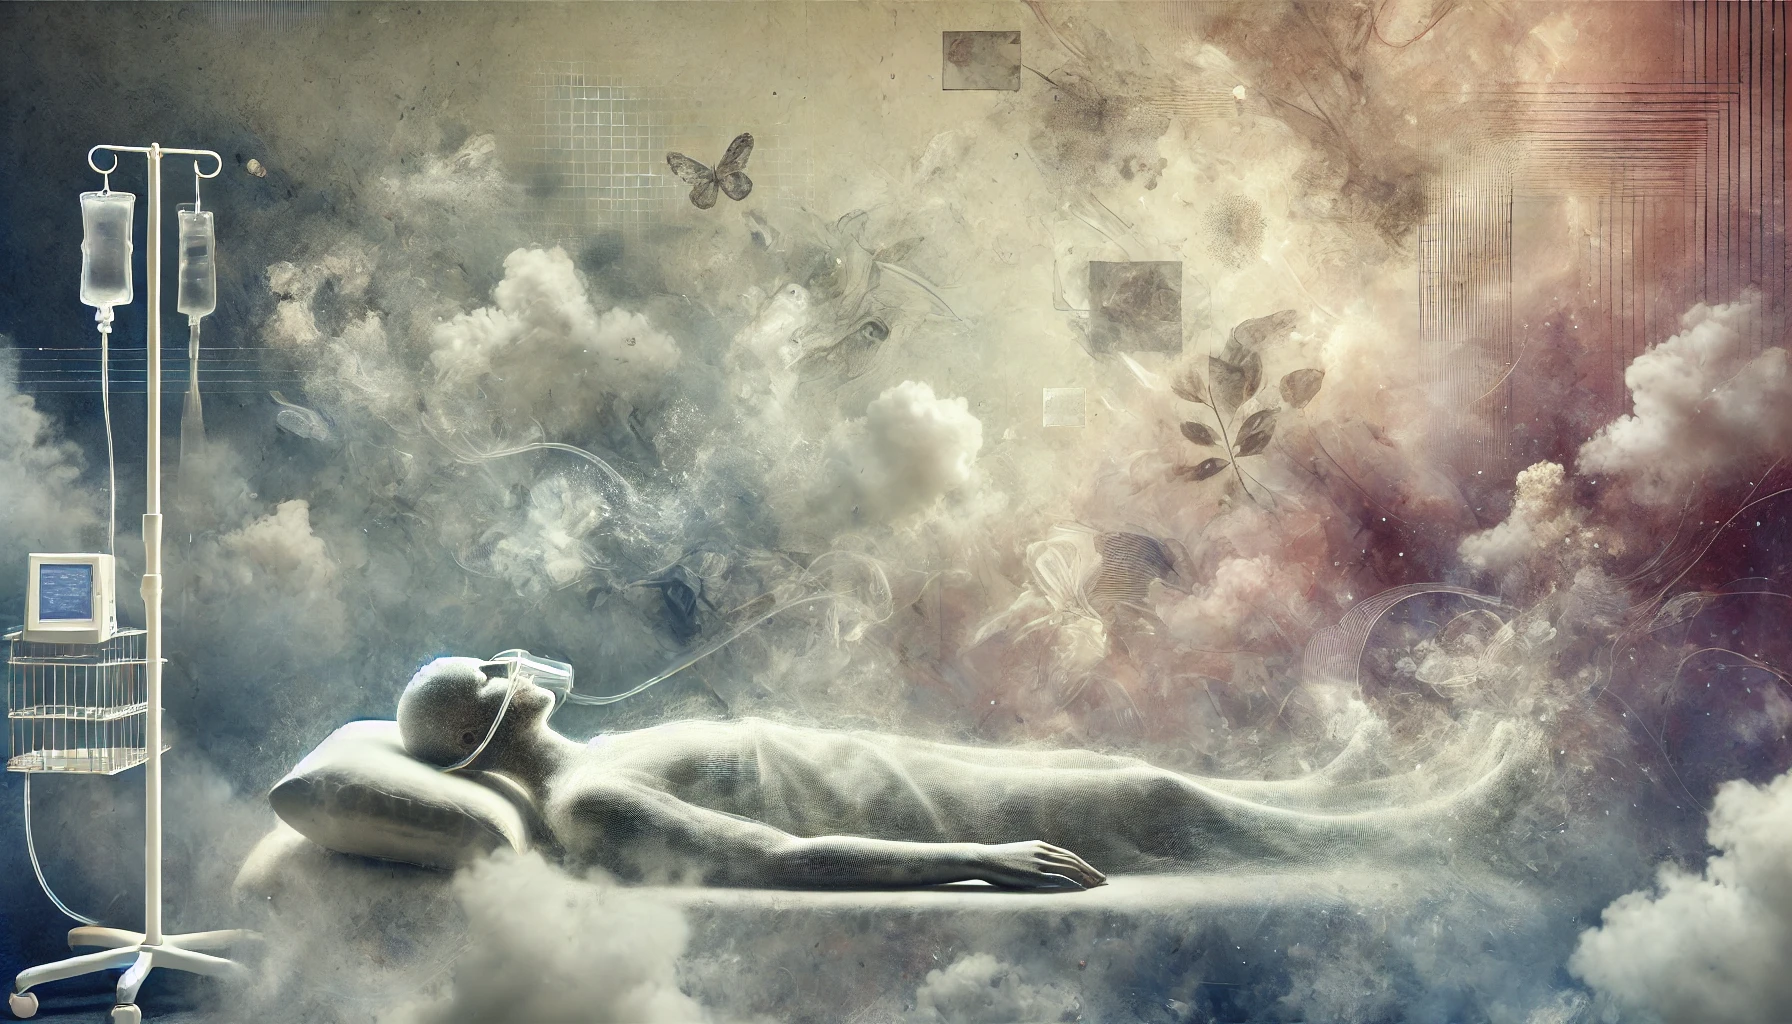
\includegraphics[width=0.8\textwidth]{anesthesia.png}

    \caption{Artistic depiction of a person under anesthesia. }
\end{figure}

The spatial organization of anesthetic effects proves particularly revealing about consciousness \cite{Lewis2012}. Rather than producing uniform suppression across neural tissues, anesthetics create specific patterns of disruption that target the networks and connections crucial for conscious processing. This anatomical specificity helps explain why consciousness can be eliminated while preserving essential physiological functions. The resulting patterns of neural activity demonstrate how consciousness requires particular forms of network organization beyond mere neural activation.

The temporal dynamics of anesthetic action provide additional insights into conscious processing \cite{Purdon2013}. The transition into unconsciousness often occurs more rapidly than emergence, revealing fundamental asymmetries in how consciousness is maintained and restored. These temporal patterns suggest that consciousness requires specific sequences of energetic organization that can be quickly disrupted but need more coordinated processes for re-establishment. The precise timing of these transitions helps illuminate the dynamic requirements for conscious processing.

The preservation of certain neural functions under anesthesia while eliminating consciousness reveals crucial distinctions in neural processing \cite{Sanders2012}. Many basic reflexes and autonomic functions continue during anesthesia, demonstrating that sophisticated neural activity can persist without supporting conscious experience. This dissociation helps identify the specific patterns of energetic coherence that consciousness requires, distinct from other forms of neural processing.

The interaction between anesthetic agents and brain rhythms reveals fundamental principles about conscious organization \cite{Steriade2003}. Different anesthetics produce characteristic changes in oscillatory patterns that correlate with the loss and recovery of consciousness. These effects suggest that proper orchestration of brain rhythms proves essential for conscious processing, while specific disruptions of these rhythmic patterns can systematically eliminate consciousness while preserving basic neural function.

The role of thalamocortical circuits in anesthetic-induced unconsciousness demonstrates key principles about conscious processing \cite{Mashour2017}. Anesthetics specifically disrupt the patterns of communication between thalamus and cortex that support conscious integration. This targeted effect on thalamocortical coherence reveals fundamental mechanisms necessary for maintaining conscious states.

The differential sensitivity of neural circuits to anesthetics provides insights into consciousness \cite{Tonner2017}. Certain neural pathways prove particularly vulnerable to anesthetic disruption, while others maintain function even at deep levels of anesthesia. This selective effect helps identify the specific circuits and mechanisms most crucial for conscious processing.

The implications of anesthetic mechanisms extend beyond clinical practice to fundamental questions about consciousness itself \cite{Alkire2008}. The ability to precisely and reversibly eliminate consciousness through specific molecular interventions demonstrates that consciousness requires particular patterns of energetic organization rather than emerging from computation alone. This understanding suggests new approaches to both studying consciousness and developing more sophisticated methods for controlling conscious states.

Perhaps most significantly, anesthesia reveals how consciousness depends on specific physical mechanisms that can be systematically disrupted \cite{Brown2010}. Unlike philosophical thought experiments about consciousness, anesthesia provides concrete evidence for the physical basis of conscious experience through reliable and reversible manipulation of conscious states. This empirical grounding proves essential for developing both theoretical understanding of consciousness and practical applications in medicine.

The study of anesthesia through ECC's framework suggests new directions for research and clinical practice \cite{Franks2008}. Rather than focusing solely on receptor binding or neural activity patterns, this perspective emphasizes how different anesthetic agents converge on disrupting specific patterns of energetic coherence necessary for consciousness. This understanding could lead to more precisely targeted anesthetic agents and better methods for monitoring depth of anesthesia.

Unlike anesthetics, which suppress consciousness, psychedelics and other psychoactive compounds modify conscious experience by altering patterns of energy flow and neural synchronization while maintaining basic coherence \cite{John2005}. These substances create distinctive alterations in consciousness through specific modulation of neural dynamics. Moving forward, we must examine how these compounds reshape conscious experience through targeted changes in brain organization and energy flow.

\section{Altered States of Consciousness}

The study of altered states reveals fundamental principles about conscious processing through examining how various compounds can profoundly modify experience while maintaining basic coherence. Unlike anesthetics, which suppress consciousness entirely, psychedelics and other psychoactive substances reshape conscious experience through specific modulation of neural dynamics and energy flows \cite{CarhartHarris2019}. These chemical interventions demonstrate how consciousness can maintain coherent organization while undergoing dramatic alterations in its qualitative character.

Classical psychedelics like LSD and psilocybin create particularly striking modifications of conscious experience through their effects on serotonin systems \cite{Nichols2016}. By activating 5-HT2A receptors, these compounds enhance neural plasticity and fundamentally alter patterns of brain synchronization. The resulting changes in default mode network activity and information integration reveal how consciousness can maintain coherent processing while operating in radically different modes. These substances demonstrate how specific molecular interventions can reliably induce profound but organized changes in conscious experience.

The role of set and setting in psychedelic experiences reveals sophisticated principles of conscious regulation \cite{Zinberg1984}. The same compounds can produce markedly different effects depending on psychological and environmental context, demonstrating how consciousness integrates multiple levels of influence in creating coherent experience. This context-dependency shows how altered states emerge from the interaction between specific molecular mechanisms and broader patterns of neural organization.

Network analysis reveals how different classes of psychoactive compounds create distinct patterns of alteration in conscious processing \cite{Preller2018}. Psychedelics tend to increase global connectivity while disrupting normal hierarchical processing, enabling enhanced cross-modal integration and novel patterns of association. These different patterns of network reorganization demonstrate how consciousness can maintain coherent function while operating through dramatically altered configurations.

The relationship between altered states and energy metabolism reveals sophisticated principles of conscious organization \cite{Vaitl2005}. Psychedelics and stimulants create distinct patterns of metabolic demand, adjusting how neural circuits utilize and distribute energy. These changes in metabolic dynamics demonstrate how consciousness can sustain coherent processing through different energetic regimes. The precise coordination between altered neural activity and energy metabolism proves essential for maintaining conscious states during these profound modifications.

The temporal dynamics of altered states demonstrate remarkable sophistication in how consciousness maintains coherence through dramatic transitions \cite{Vollenweider2020}. The onset, peak effects, and gradual resolution of psychedelic experiences reveal how conscious processing can undergo profound reorganization while preserving basic stability. These temporal patterns suggest that consciousness possesses intrinsic mechanisms for maintaining coherent function even during radical alterations in its organizing principles.

\begin{figure}[h]
    \centering
    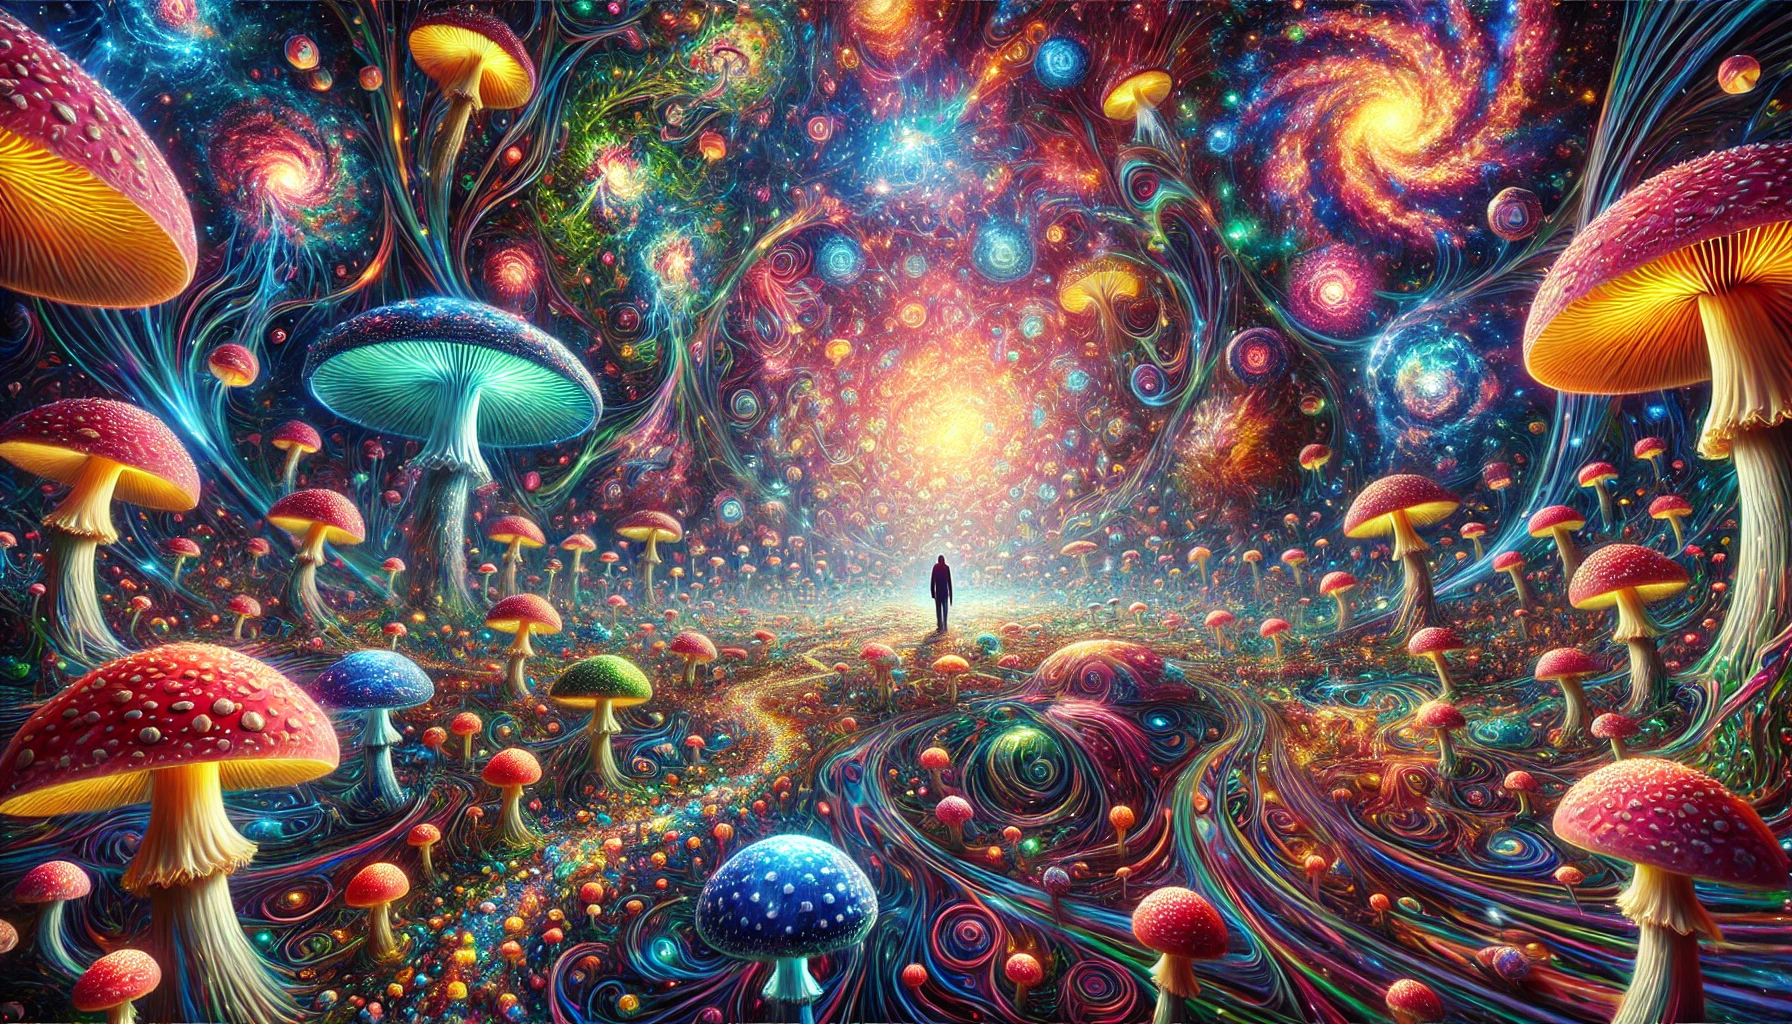
\includegraphics[width=0.8\textwidth]{mushroom_trip.png}

    \caption{A mushroom trip}
\end{figure}

The interaction between different neurotransmitter systems during altered states reveals complex principles of conscious regulation \cite{Ludwig1966}. Psychedelics influence not only serotonin systems but also modulate glutamate release and neural plasticity, creating cascading effects across multiple signaling pathways. These sophisticated patterns of chemical interaction demonstrate how consciousness emerges from coordinated activity across multiple molecular systems rather than single neurotransmitter effects.

Changes in perception during altered states illuminate fundamental aspects of how consciousness constructs experience \cite{Dittrich2010}. The modification of sensory processing, emotional responses, and cognitive associations reveals how consciousness actively organizes information rather than passively receiving it. The maintenance of coherent experience despite dramatic alterations in these organizing principles demonstrates the remarkable flexibility of conscious processing.

The relationship between altered states and the default mode network proves particularly revealing \cite{CarhartHarris2019}. Psychedelics can fundamentally reshape activity in this network while preserving broader conscious function, suggesting that even core aspects of self-experience arise from specific patterns of energetic organization that can be systematically modified. These alterations in self-processing reveal how consciousness maintains coherent experience even when fundamental aspects of cognition become profoundly altered.

Memory formation during altered states demonstrates sophisticated principles of conscious integration \cite{Hobson2007}. Despite profound changes in experience, consciousness maintains the ability to encode and later recall these altered states, suggesting that coherent memory formation can persist even during dramatic reorganization of conscious processing. This preservation of memory function reveals how consciousness maintains essential capabilities even while operating in radically different modes.

The clinical implications of understanding altered states through ECC's framework suggest new therapeutic approaches for various psychological conditions \cite{Vollenweider2020}. The capacity of psychedelics to enable coherent yet profoundly reorganized states of consciousness indicates potential pathways for treating disorders that involve rigid or maladaptive patterns of neural organization. This perspective helps explain both the therapeutic potential of psychedelic compounds and the importance of carefully managed contexts for their administration.

The role of cultural frameworks in shaping altered states reveals important principles about conscious organization \cite{Winkelman2010}. While the underlying neural mechanisms may be similar, the interpretation and expression of psychedelic experiences vary dramatically across cultural contexts. This interaction between biological and cultural factors demonstrates how consciousness integrates multiple levels of organization in creating coherent experience.

Perhaps most significantly, the study of altered states through ECC's framework reveals fundamental principles about the nature of conscious processing \cite{Preller2018}. Rather than representing random disruption of normal function, these states demonstrate how consciousness can maintain coherent organization while operating through radically different patterns of energetic dynamics. This understanding challenges simplified models of consciousness while suggesting new approaches to both scientific investigation and therapeutic application.

The implications extend beyond clinical practice to fundamental questions about the potential range of conscious experience \cite{Wulff2014}. The remarkable variety of altered states achievable through specific molecular interventions suggests that normal waking consciousness represents just one of many possible coherent configurations of neural dynamics. This perspective opens new avenues for understanding both the flexibility and constraints of conscious processing in biological systems.

Unlike pharmacologically induced alterations, trance states and ecstatic experiences represent unique modifications of consciousness that can occur without external intervention \cite{Eliade1964}. These states reveal how internal regulation of energy dynamics can produce profound alterations in conscious experience through sophisticated management of neural coherence \cite{Farthing1992}. Moving forward, we must examine how these endogenous mechanisms reshape conscious experience through voluntary control of brain organization and energy flow.

\section{Trance and Ecstasis}

Trance states and ecstatic experiences reveal unique modifications of consciousness achievable through internal regulation rather than external intervention. Where psychedelics and other compounds alter consciousness through direct molecular action, trance states demonstrate how sophisticated management of neural energetics can produce profound alterations in conscious experience through voluntary control \cite{Rouget1985}. These internally generated modifications of consciousness illuminate fundamental principles about how biological systems can maintain coherent processing while operating in radically altered configurations.

Physiological changes during trance states demonstrate remarkable sophistication in conscious regulation \cite{Becker2004}. Through controlled modulation of breathing patterns, heart rate variability, and autonomic balance, practitioners can systematically alter their conscious experience while maintaining coherent organization. These coordinated physiological changes create specific patterns of brain wave activity that support altered states while preserving essential functional stability. The resulting modifications in consciousness emerge from precise management of biological rhythms rather than random perturbation.

The energy dynamics of trance states reveal particularly sophisticated principles of neural regulation \cite{Lewis2003}. Unlike the broad disruptions caused by pharmacological interventions, trance states involve highly organized patterns of oscillatory activity that maintain specific forms of coherence while enabling profound alterations in experience. These coordinated changes in neural energetics demonstrate how consciousness can achieve dramatic modifications through careful management of intrinsic biological rhythms.

Network reorganization during trance reveals fundamental principles about conscious flexibility \cite{Wier2009}. Reduced activity in the default mode network, enhanced interoceptive processing, and modified sensory gating create distinctive patterns of neural activation that support profound alterations in conscious experience. These changes in network organization demonstrate how internal regulation can reshape conscious processing while maintaining essential coherence. The resulting states enable forms of experience typically inaccessible during normal waking consciousness.

The relationship between trance states and bodily awareness illuminates sophisticated mechanisms of conscious control \cite{Goodman1988}. Through sustained attention to interoceptive signals and careful regulation of physiological processes, practitioners can systematically modify their conscious experience while maintaining organized function. These internally generated alterations demonstrate how consciousness can achieve profound modifications through voluntary regulation rather than external intervention.

The phenomenology of trance states reveals important principles about conscious organization \cite{Lapassade1990}. Practitioners often report experiences of altered self-boundaries, modified temporal perception, and enhanced awareness of subtle bodily processes. These changes in conscious experience emerge from systematic modification of neural dynamics rather than random disruption. The resulting alterations demonstrate how consciousness can maintain coherent function while operating through radically different patterns of self-organization.

\begin{figure}[h]
    \centering
    
\includegraphics[width=0.8\textwidth]{trance.png}

    \caption{A shaman in a state of trance}
\end{figure}

The distinction between different forms of trance illuminates multiple pathways for conscious modification \cite{Bourguignon1973}. Meditative states, shamanic journeying, and possession trance each involve distinct patterns of physiological and neural regulation that produce unique alterations in conscious experience. These various forms of trance reveal how consciousness can achieve profound modifications through different combinations of internal control. The diversity of possible trance states demonstrates the remarkable flexibility of conscious processing.

The role of cultural frameworks in shaping trance experiences proves particularly significant \cite{Lewis2003}. While the underlying neural mechanisms may be similar, the interpretation and expression of trance states vary dramatically across cultural contexts. This interaction between biological and cultural factors demonstrates how consciousness integrates multiple levels of organization in creating coherent experience. The resulting states reflect both universal principles of neural organization and specific cultural patterns of meaning.

The temporal dynamics of trance induction reveal sophisticated principles of conscious regulation \cite{Turner1992}. Rather than sudden shifts in experience, trance states typically develop through graduated stages of physiological and neural reorganization. This progressive modification of conscious processing enables stable transitions between radically different states of awareness. The careful management of these transitions demonstrates how consciousness can maintain coherent function while undergoing fundamental reorganization.

The relationship between trance states and memory formation shows interesting patterns of conscious integration \cite{Jilek1982}. Unlike some drug-induced states, trance experiences often remain accessible to later recall while incorporating elements of both ordinary and extraordinary awareness. This preservation of memory function during profound alterations in consciousness reveals how biological systems can maintain essential capabilities while operating in radically different modes.

The role of trance states in therapeutic contexts reveals promising applications of this understanding \cite{Crapanzano1973}. The capacity for consciousness to achieve profound yet controlled alterations through internal regulation suggests new approaches to treating various psychological conditions. Rather than relying solely on external interventions, therapeutic practices might develop more sophisticated methods for enhancing conscious self-regulation through disciplined practice and cultural scaffolding.

The relationship between trance and social context demonstrates sophisticated principles of conscious modification \cite{Houseman1998}. Many traditional trance practices occur within structured social settings that help guide and stabilize altered states of consciousness. This social scaffolding reveals how conscious regulation can be enhanced through cultural frameworks and interpersonal support.

Perhaps most significantly, the study of trance and ecstatic states through ECC's framework reveals fundamental principles about the nature of conscious processing itself \cite{Rouget1985}. The remarkable capacity for internally regulated alterations in consciousness demonstrates how biological systems can maintain coherent function while operating through radically different configurations. This understanding challenges purely computational approaches to consciousness while suggesting new directions for both scientific investigation and therapeutic application.

The implications extend beyond traditional contexts to broader questions about human potential for conscious regulation \cite{Lewis2003}. The sophisticated control demonstrated in trance states suggests that normal waking consciousness represents just one of many possible coherent configurations. This perspective opens new avenues for understanding both the flexibility and constraints of conscious processing in biological systems.

Moving beyond trance states to examine another fundamental aspect of consciousness, we must consider how specific patterns of sensory integration can create unique forms of conscious experience through synaesthesia \cite{Goodman1988}. Unlike metaphorical associations or learned connections, synaesthetic experiences demonstrate how specific patterns of neural architecture can enable direct crossing of sensory boundaries while maintaining coherent conscious states.

\section{Synaesthesia}

The phenomenon of synaesthesia, where stimulation in one sensory modality reliably triggers experiences in another, offers compelling evidence for how consciousness emerges from patterns of energetic coherence maintained through biological organization. Unlike metaphorical associations or learned connections, synaesthetic experiences demonstrate how specific patterns of neural architecture can enable direct crossing of sensory boundaries while maintaining coherent conscious states \cite{Ramachandran2001}.

The molecular basis of synaesthesia reveals sophisticated principles about conscious organization \cite{Hubbard2005}. Different regions of the brain maintain unique transcriptomic profiles that typically ensure separation between sensory modalities. In synaesthetes, variations in these molecular patterns create conditions where energy flows can cross typical boundaries while maintaining stable organization. These modified patterns of neural architecture demonstrate how conscious experiences emerge from specific configurations of biological organization rather than abstract computation.

The stability of synaesthetic associations proves particularly significant for understanding conscious processing \cite{Dixon2004}. Individual synaesthetes maintain consistent relationships between triggering stimuli and cross-modal experiences over time, suggesting that these altered patterns of conscious organization achieve remarkable stability once established. This consistency reveals how consciousness can maintain novel forms of sensory integration while preserving coherent function. The resulting experiences demonstrate consciousness's capacity for stable yet unconventional organizations of sensory processing.

The diversity of synaesthetic forms illuminates different possibilities for conscious organization \cite{Ward2013}. While some individuals experience colors in response to sounds, others might perceive tastes from shapes or spatial arrangements from temporal sequences. These various manifestations of cross-modal experience reveal how consciousness can achieve multiple forms of stable sensory integration through different patterns of neural organization. The resulting variety of synaesthetic experiences demonstrates the remarkable flexibility of conscious processing while maintaining coherent function.

The developmental trajectory of synaesthesia suggests important principles about conscious organization \cite{Simner2012}. These cross-modal associations often emerge during critical periods of brain development, when patterns of neural connectivity remain particularly plastic. The timing of synaesthetic development reveals how consciousness establishes stable patterns of sensory integration through specific periods of biological organization. This temporal specificity demonstrates the importance of developmental processes in shaping conscious experience.

The neural basis of synaesthetic experience reveals fundamental principles about how consciousness integrates different forms of sensory information \cite{Nunn2002}. Brain imaging studies show that synaesthetes' experiences correlate with activation of both primary sensory areas and higher-order integration regions, demonstrating how altered patterns of neural connectivity can create stable forms of cross-modal experience.

\begin{figure}[h]
    \centering
    
\includegraphics[width=0.8\textwidth]{synaesthesia.png}

    \caption{Synaesthesia - an interplay of senses}
\end{figure}

The study of synaesthetic development reveals crucial insights about how consciousness establishes stable patterns of sensory integration \cite{Barnett2008}. These cross-modal associations typically emerge during critical periods of brain development, when neural plasticity allows for the establishment of novel patterns of sensory integration. The timing and progression of synaesthetic development demonstrates how consciousness relies on specific biological conditions to establish and maintain coherent patterns of cross-modal experience.

The directionality of synaesthetic associations proves particularly revealing about conscious organization \cite{Eagleman2009}. While a grapheme might consistently trigger a specific color experience, the reverse typically does not occur - colors do not automatically evoke specific letters or numbers. This asymmetry suggests that consciousness maintains specific hierarchies in sensory integration, even when establishing novel patterns of cross-modal association. The resulting organizational principles demonstrate how consciousness preserves certain fundamental constraints while enabling novel forms of sensory integration.

Individual differences in synaesthetic experience reveal important principles about conscious variation \cite{Dixon2004}. While some synaesthetes experience vivid, externally projected associations, others describe more subtle, internally experienced connections. These variations in phenomenal quality demonstrate how consciousness can maintain different degrees of perceptual integration while preserving the stability and consistency characteristic of synaesthetic experience.

The relationship between synaesthesia and broader cognitive function reveals sophisticated principles of neural organization \cite{Kadosh2007}. Synaesthetes often demonstrate enhanced memory for information related to their cross-modal associations, suggesting that these additional patterns of sensory integration can support rather than interfere with cognitive processing. This cognitive enhancement demonstrates how novel patterns of conscious organization can provide functional advantages while maintaining coherent processing.

Neural imaging studies of synaesthetes reveal specific patterns of brain activity that correspond to their unique sensory experiences \cite{Nunn2002}. These activation patterns demonstrate how consciousness can establish stable forms of cross-modal integration through specific modifications of neural architecture. The resulting patterns of brain activity reveal how consciousness achieves novel forms of sensory integration through precise alterations in neural organization rather than random cross-activation.

The interaction between synaesthetic experiences and attention reveals sophisticated principles of conscious control \cite{Mattingley2001}. While synaesthetic associations occur automatically, their intensity and salience can be modulated by attentional focus. This relationship demonstrates how consciousness can maintain stable patterns of cross-modal integration while enabling dynamic control over their expression.

The implications of synaesthesia for understanding consciousness extend beyond individual cases to fundamental principles about neural organization \cite{Ramachandran2001}. The ability of consciousness to maintain stable cross-modal associations while preserving normal sensory processing demonstrates remarkable sophistication in managing multiple streams of sensory information. This capacity for parallel processing reveals how consciousness can establish novel patterns of integration while maintaining essential functional organization.

The functional diversity of synaesthetic experience reveals fundamental organizing principles of conscious processing \cite{Grossenbacher2001}. Different forms of synaesthesia utilize distinct patterns of neural connectivity to achieve specific types of cross-modal integration while maintaining broader perceptual coherence. This architectural specialization demonstrates how biological systems can achieve both local specificity and global integration through precise patterns of neural organization \cite{Ward2013}.

Perhaps most significantly, synaesthesia demonstrates how consciousness emerges from specific patterns of neural architecture that enable stable forms of cross-modal integration \cite{Hubbard2005}. Rather than representing mere associations or learned connections, synaesthetic experiences reveal how particular configurations of neural organization can create reliable and consistent forms of conscious experience. This understanding suggests new approaches to studying both normal sensory processing and potential therapeutic applications based on enhancing sensory integration.

In the spirit of expanding on non-standard experiences in the general population, we will now delve deeper into peculiar conditions of the visual field such as visual snow and tetrachromacy.

\section{Visual Snow}

Visual snow offers a unique window into how ECC's framework can explain perceptual phenomena that challenge traditional computational models of consciousness. This condition, characterized by continuous visual static perceived across the entire visual field \cite{Puledda2020}, provides compelling evidence for how consciousness emerges from and remains grounded in underlying patterns of energetic coherence.

The phenomenon demonstrates several key principles of ECC's framework. Unlike typical visual processing, which involves organized patterns of neural activity representing external stimuli, visual snow appears to reveal the background energy dynamics that typically remain below the threshold of conscious awareness. This aligns with evidence suggesting that visual snow may represent a fundamental dysrhythmia in thalamocortical circuits \cite{Lauschke2016}, affecting how the brain maintains coherent visual representations.

Recent clinical investigations have established visual snow as a distinct neurological condition rather than merely a symptom of other disorders \cite{Schankin2014}. The persistence of visual static across different lighting conditions and its independence from external stimuli suggest that it emerges from alterations in how the brain maintains coherent visual states rather than from disruptions in early sensory processing \cite{Bessero2014}.

Through ECC's framework, visual snow can be understood as a modification in how the brain achieves and maintains coherent energy states in visual processing regions. The continuous, grainy quality of the phenomenon reflects underlying patterns of energetic activity that normally remain integrated into seamless visual experience. This interpretation aligns with predictive processing accounts of perception \cite{Clark2013}, suggesting that visual snow represents a disruption in how the brain maintains stable perceptual predictions through coherent energy dynamics.

The relationship between visual snow and other perceptual phenomena becomes particularly clear through ECC's emphasis on energetic coherence. The frequent co-occurrence of persistent after-images and enhanced pattern sensitivity in visual snow patients \cite{Puledda2020} suggests broader alterations in how visual processing regions maintain coherent states. These associated symptoms indicate that visual snow involves fundamental changes in how the brain organizes visual experience through patterns of energetic coherence rather than simple sensory disruption.

This understanding has important implications for both theoretical models of consciousness and clinical approaches to visual snow. Rather than treating the condition as a processing error or pathological activation, ECC suggests it represents an alternative configuration of how consciousness organizes visual experience through energetic coherence. This perspective aligns with embodied approaches to perception \cite{ORegan2001} while providing a specific mechanism - disrupted patterns of energetic coherence - through which altered visual experiences can emerge.

The framework also suggests why visual snow proves resistant to traditional treatments targeting neurotransmitter systems. If the condition represents a fundamental reorganization of how visual regions maintain coherent states, interventions (should they even be required or desired) may need to focus on restoring appropriate patterns of energetic coherence rather than simply modulating neural activity. This understanding could guide the development of new therapeutic approaches based on supporting stable patterns of visual coherence.

Visual snow thus serves as a crucial test case for understanding how consciousness emerges from patterns of energetic coherence in neural systems. The condition demonstrates both the flexibility and constraints of conscious visual processing while suggesting new approaches to investigating and treating disorders of perceptual organization.

\begin{figure}[h]
    \centering
    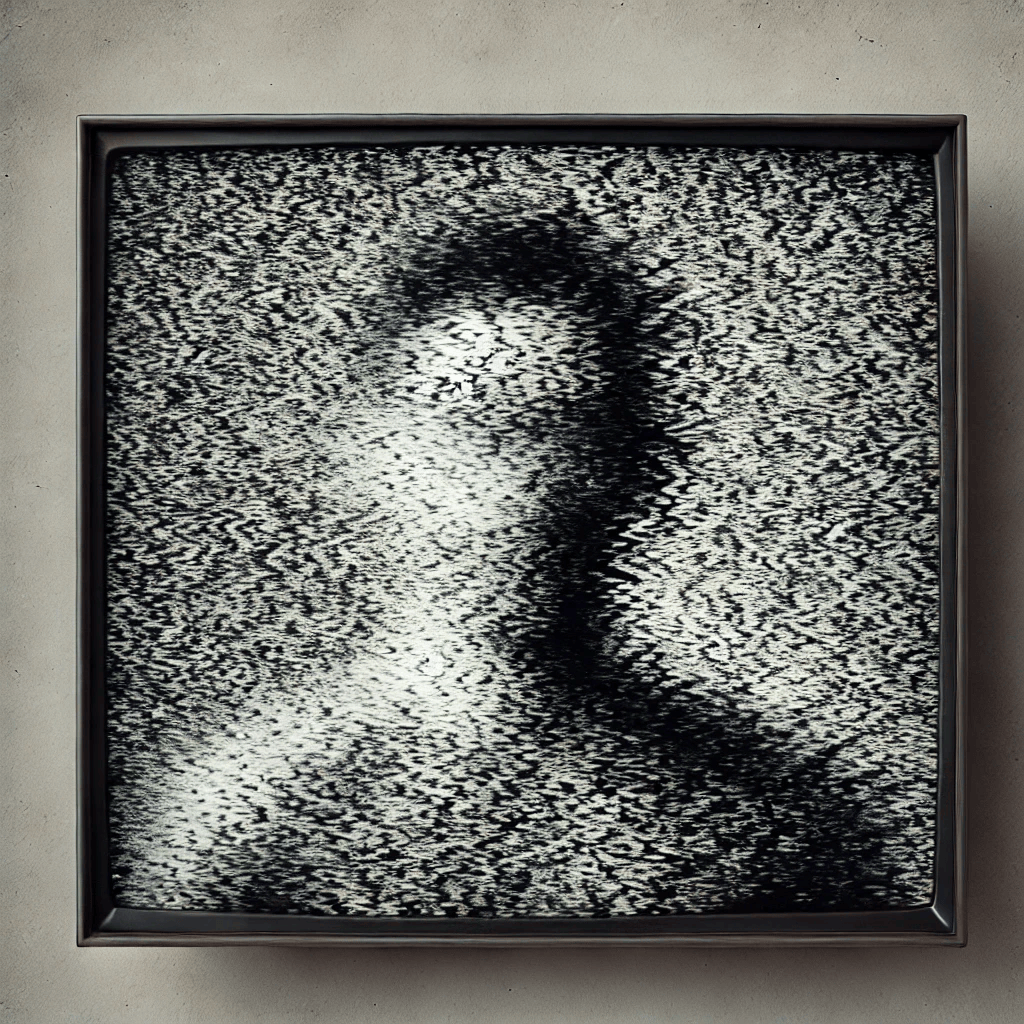
\includegraphics[width=0.8\textwidth]{snow.png}

    \caption{An exaggerated depiction of visual snow.}
\end{figure}

Building on this foundation, we can further explore how visual snow illuminates fundamental principles of perceptual organization through the lens of energetic coherence. Traditional predictive coding accounts \cite{Rao1999, Friston2009} suggest that perception emerges from hierarchical prediction processes, but ECC extends this understanding by grounding these processes in patterns of energetic coherence that maintain stable perceptual states.

The phenomenology of visual snow provides crucial insights into how consciousness maintains coherent perceptual fields. Rather than representing random noise in visual processing, the consistent and organized nature of visual snow - its characteristic density, temporal dynamics, and field-like distribution - suggests disruption in how the brain maintains background patterns of energetic coherence. This aligns with enactive approaches to perception \cite{Varela1991} while providing specific mechanisms through which perceptual experiences emerge from neural dynamics.

Recent theoretical work in sensorimotor contingencies \cite{Seth2014} helps explain why visual snow remains relatively stable across different viewing conditions and contexts. Unlike hallucinations or other visual phenomena that vary with attention or environmental conditions, visual snow maintains consistent characteristics that suggest fundamental alterations in how visual consciousness achieves coherent organization. This stability points to changes in the underlying energetic patterns that support visual experience rather than disruptions in higher-level processing.

The relationship between visual snow and broader theories of consciousness becomes particularly clear when considering how the condition affects perceptual presence - the sense that perceived objects are real and present in the environment \cite{Seth2014}. While visual snow patients maintain normal perception of external objects, the constant presence of visual static reveals how consciousness simultaneously maintains multiple layers of perceptual organization through distinct patterns of energetic coherence.

This multi-level organization of visual consciousness aligns with philosophical accounts of perception that emphasize its active, constitutive nature \cite{Noe2004}. Visual snow demonstrates how consciousness doesn't simply process sensory inputs but actively maintains coherent perceptual states through sophisticated patterns of energetic organization. The condition reveals these organizational processes by making typically implicit aspects of visual processing explicitly present in consciousness.

The theoretical significance of visual snow extends beyond clinical understanding to fundamental questions about the nature of conscious perception. The condition challenges purely representational theories of consciousness \cite{Metzinger2003} by demonstrating how perceptual experience emerges from and remains grounded in patterns of energetic coherence rather than abstract information processing. This suggests new approaches to investigating both normal perception and its alterations in various conditions.

The relationship between visual snow and other perceptual variations provides deeper insight into how consciousness maintains coherent visual states through patterns of energetic organization. Much like color perception demonstrates structured relationships that resist arbitrary reconfiguration \cite{Palmer1999}, visual snow reveals fundamental aspects of how visual consciousness achieves stable organization through coherent energy dynamics.

This perspective aligns with research suggesting that perception emerges from structured relationships within neural systems rather than arbitrary mappings between stimuli and experience \cite{Thompson1995}. Visual snow demonstrates how these relationships can be systematically altered while maintaining basic coherence - the visual static remains organized and stable even as it modifies normal visual experience. This structured modification suggests that consciousness operates through constrained patterns of energetic coherence rather than through unconstrained information processing.

The condition also illuminates debates about the plasticity of perceptual categories \cite{VanBrakel1993}. While visual snow represents a dramatic alteration in visual experience, it maintains consistent characteristics across individuals and contexts, suggesting fundamental constraints on how consciousness can organize visual experience through patterns of energetic coherence. These constraints help explain both the stability of normal perception and the specific ways it can be altered in various conditions.

Understanding visual snow through ECC's framework provides new perspective on classical problems in philosophy of perception, such as the relationship between subjective experience and neural activity \cite{Tye2000}. Rather than requiring a solution to the hard problem of consciousness, ECC suggests that visual snow reveals how conscious experience emerges directly from patterns of energetic coherence in neural systems. This helps explain both the phenomenal character of visual snow and its resistance to reduction to purely computational descriptions.

The implications extend beyond theoretical understanding to practical approaches for investigating and treating perceptual disorders. By recognizing how visual snow emerges from altered patterns of energetic coherence rather than simple processing disruptions, researchers and clinicians might develop more effective interventions focused on restoring appropriate patterns of perceptual organization. This could lead to novel therapeutic approaches that target the underlying organizational principles of visual consciousness rather than just its surface manifestations.

Visual snow thus serves as a crucial case study for understanding how consciousness emerges from and maintains coherent perceptual states through sophisticated patterns of energetic organization. The condition reveals fundamental principles about how consciousness operates while suggesting new directions for both theoretical research and clinical practice. This understanding helps bridge the gap between subjective experience and neural dynamics while providing concrete approaches to investigating and treating disorders of conscious perception.

\section{Color perception}

Color perception, like visual snow, also presents a unique challenge for theories of consciousness, revealing fundamental principles about how neural systems achieve coherent representations of sensory qualities. The apparent universality of certain aspects of color experience, combined with clear evidence of cultural and individual variation \cite{Davidoff2015}, provides crucial insight into how consciousness maintains stable perceptual states while allowing for structured variation.

Recent advances in understanding the biological basis of color perception \cite{ConwayLivingstone2021} demonstrate how specific neural architectures support the emergence of coherent color experiences. Through ECC's framework, these neural mechanisms can be understood not as merely computing color values, but as maintaining specific patterns of energetic coherence that give rise to stable color experiences. This perspective helps bridge the gap between neurobiological mechanisms and phenomenal experience.

The question of color categorization proves particularly revealing about how consciousness organizes perceptual experience. While early theories suggested universal bases for color categories, contemporary research reveals a more complex picture \cite{KayRegier2003}. Cross-cultural studies demonstrate both systematic commonalities and significant variations in how different societies organize color experience \cite{MacLaury1997}. Through ECC's framework, these patterns can be understood as emerging from the interaction between shared biological constraints on energetic coherence and culturally shaped patterns of perceptual organization.

The investigation of color vision in carriers of anomalous trichromacy provides crucial evidence about how conscious color experience emerges from patterns of neural organization \cite{JordanMollon1993}. These studies reveal how variations in photopigment genes can create subtle but significant differences in color discrimination, suggesting that conscious color experience depends on specific patterns of energetic coherence shaped by molecular-level variations in neural architecture.

Traditional color vision theory focused primarily on the three standard cone types, but research has revealed greater complexity in how the visual system achieves coherent color representations. The discovery of individuals with enhanced color discrimination capabilities \cite{Jameson2001} demonstrates how consciousness can maintain more sophisticated patterns of color differentiation when supported by appropriate neural architecture. This aligns with ECC's emphasis on how conscious experiences emerge from specific patterns of energetic coherence rather than abstract computational processes.

Through ECC's framework, color perception can be understood as emerging from structured patterns of energetic coherence that remain stable across individuals while allowing for systematic variation. This helps explain both the commonalities in color experience across cultures and the specific ways that color perception can vary between individuals and populations. The framework suggests that color experience is neither purely subjective nor simply determined by wavelength detection, but emerges from sophisticated patterns of neural organization that support coherent perceptual states.

The relationship between color perception and consciousness thus reveals fundamental principles about how phenomenal experiences emerge from neural dynamics. Rather than requiring a solution to the traditional mind-body problem, ECC suggests that color experiences arise directly from patterns of energetic coherence maintained by specialized neural architectures. This understanding helps explain both the stability and variability of color perception while suggesting new approaches to investigating perceptual consciousness.

Examining how color experience achieves stability while maintaining flexibility provides crucial insight into consciousness itself. Research on color relationalism suggests that perceptual qualities emerge not from simple stimulus-response mappings but from structured relationships within neural systems \cite{ByrneHilbert2017}. Through ECC's framework, these relationships can be understood as patterns of energetic coherence that support stable yet flexible color experiences.

The geometry of color perception proves particularly revealing about how consciousness organizes sensory experiences. Recent mathematical analyses of homogeneous color spaces \cite{Provenzi2020} demonstrate that color experience exhibits intrinsic structural constraints that cannot be reduced to arbitrary mappings. These geometric properties suggest fundamental principles about how consciousness achieves coherent perceptual states through specific patterns of energetic organization. They reveal intrinsic asymmetries and structural relationships that challenge traditional philosophical thought experiments like the inverted spectrum hypothesis \cite{Block1990}. The geometric constraints shown by this line of research suggest that color experiences cannot be arbitrarily inverted or reorganized while maintaining coherent relationships between perceptual qualities and their underlying neural dynamics.

The investigation of color categorization across cultures \cite{Kay2003} mentioned above further illuminates how consciousness achieves stable organization within these geometric constraints. While cultural variations exist in color naming and categorization, these differences operate within structural limitations imposed by the architecture of human color perception. Through ECC's framework, these patterns can be understood as emerging from fundamental constraints on how consciousness can maintain coherent perceptual states.

Research on synaesthetic experiences involving color \cite{HarrisonBaronCohen1997} provides additional insight into how consciousness integrates chromatic information with other perceptual qualities. The systematic nature of color-based synaesthesia suggests that even novel associations between sensory modalities must respect underlying geometric constraints in how consciousness organizes color experience. This structured flexibility demonstrates how consciousness maintains coherent perceptual states while enabling diverse patterns of sensory integration.

The philosophical implications of these findings extend beyond specific questions about color perception to fundamental issues in consciousness studies \cite{Palmer1999}. The existence of geometric constraints on color experience, combined with evidence from tetrachromacy and cross-cultural research, suggests that conscious experiences emerge from structured patterns of energetic coherence that cannot be arbitrarily reorganized. This challenges both radical relativist accounts of perception and simple computational models of consciousness.

Evolutionary considerations highlight how color consciousness emerges from specific neural architectures shaped by biological constraints. The development of trichromatic vision in primates \cite{Neitz2017} demonstrates how consciousness achieves coherent color representation through specialized neural mechanisms that support specific patterns of energetic organization. This evolutionary perspective helps explain both the commonalities in color experience across individuals and the specific ways it can vary between species.

Comparative studies reveal remarkable diversity in how different organisms achieve coherent color representation. Research on avian tetrachromacy \cite{Wilkins2020} demonstrates how neural systems can support forms of color consciousness that transcend human perceptual capabilities. These findings align with ECC's emphasis on how conscious experiences emerge from specific patterns of energetic coherence rather than abstract computational processes.

The investigation of anomalous color vision provides additional insight into how consciousness maintains coherent perceptual states. Studies of individuals with variant photopigment genes \cite{Jordan2010} reveal how subtle alterations in neural architecture can create systematic differences in color experience while maintaining overall perceptual coherence. This demonstrates how consciousness achieves stable color representation through sophisticated patterns of energetic organization that can accommodate significant variation in underlying neural mechanisms.

The relationship between color perception and neural architecture reveals fundamental principles about how consciousness emerges from biological systems. Rather than representing arbitrary mappings between stimuli and sensations, color experience reflects sophisticated patterns of energetic coherence shaped by both evolutionary history and individual development. This understanding helps bridge the gap between subjective experience and neural dynamics while suggesting new approaches to investigating perceptual consciousness.

The dimensionality of color vision takes on particular significance when examined through ECC's framework. Research on the biological basis of color discrimination \cite{Jacobs2018} demonstrates how neural systems achieve coherent representation of multiple color dimensions through specific patterns of energetic organization. This multidimensional organization helps explain both the richness of color experience and the specific constraints on how consciousness can represent chromatic relationships.

The implications of color perception research extend beyond individual variation to fundamental questions about the structure of conscious experience. The study of tetrachromacy, particularly in individuals possessing multiple opsin genes \cite{Jameson2001}, reveals how expanded color perception requires not just additional photoreceptors but appropriate neural architecture to support coherent representation of an enhanced perceptual space. This demonstrates how conscious experiences emerge from specific patterns of energetic coherence that must maintain stability across multiple perceptual dimensions.

Through this lens, color perception emerges not as a simple mapping between wavelengths and sensations, but as a sophisticated achievement of consciousness operating within specific geometric and biological constraints. The stability of color relationships, the possibility of enhanced color vision through tetrachromacy, and the structured nature of cultural variations all point to fundamental principles about how consciousness maintains coherent perceptual states through patterns of energetic organization that respect intrinsic geometric constraints.

This understanding helps resolve longstanding debates about the nature of color experience while suggesting new approaches to investigating consciousness itself. Rather than requiring either pure objectivism about color or complete perceptual relativism, ECC suggests how structured patterns of energetic coherence can give rise to stable yet flexible perceptual experiences that remain grounded in physical reality while allowing for systematic variation between individuals and across cultures.

\section{Music and Auditory Experience}

The relationship between music and consciousness reveals fundamental principles about how neural systems achieve and maintain coherent experiential states across time. Unlike static perceptual experiences, music requires the brain to organize complex temporal patterns while integrating multiple streams of auditory information into unified conscious experiences \cite{Janata2002}. Through ECC's framework, these musical experiences can be understood as emerging from sophisticated patterns of energetic coherence that span multiple temporal and processing scales.

Recent research in music cognition demonstrates how neural systems achieve this temporal integration through dynamic attending processes \cite{Large1999}. Rather than simply processing sequential auditory events, the brain actively maintains coherent states that enable prediction and anticipation of musical patterns. This aligns with ECC's emphasis on how consciousness emerges from organized patterns of energetic coherence rather than mere information processing.

The relationship between music and emotion proves particularly revealing about how consciousness maintains coherent experiential states. Studies of musical emotion demonstrate that affective responses emerge through complex interactions between neural systems \cite{Thompson2010}, suggesting that musical experiences involve patterns of energetic coherence that span both auditory processing and emotional regulation networks. This multi-level integration helps explain music's remarkable capacity to evoke powerful emotional responses while maintaining coherent perceptual organization.

Cross-cultural research in music cognition \cite{Patel2010} reveals both universal patterns and cultural variations in how consciousness organizes musical experience. While certain aspects of musical processing appear to reflect shared biological constraints, the specific ways that different cultures organize musical experience demonstrate how consciousness can achieve coherent states through various patterns of energetic organization. This structured flexibility aligns with ECC's emphasis on how conscious experiences emerge from specific yet variable patterns of neural coherence.

The neural architecture supporting musical experience demonstrates remarkable sophistication in maintaining coherent states across multiple processing streams \cite{Zatorre2007}. Studies of music perception and production reveal how the brain coordinates auditory, motor, and emotional systems through precise temporal relationships. These coordinated patterns of neural activity can be understood through ECC as creating stable yet dynamic fields of conscious experience that enable both perception and performance of music.

Recent theoretical work on embodied music cognition \cite{Krueger2009} suggests that musical experiences emerge from active engagement rather than passive processing. This aligns with ECC's framework by emphasizing how consciousness achieves coherent musical states through dynamic patterns of organization that span perception, action, and emotional response. The resulting integration helps explain both the immediacy of musical experience and its capacity to coordinate complex behavioral responses.

Musical rhythm and entrainment provide particularly clear examples of how consciousness maintains coherent states through time \cite{Clayton2005}. The brain's capacity to synchronize neural activity with musical patterns demonstrates sophisticated mechanisms for achieving temporal coherence across multiple processing scales. These mechanisms support both perception of musical structure and coordination of motor responses, revealing fundamental principles about how consciousness organizes temporal experience through patterns of energetic coherence.

This understanding of music through ECC's framework suggests new approaches to investigating both normal musical experience and its alterations in various neurological conditions \cite{Schaefer2014}. Rather than focusing solely on information processing or pattern recognition, research might productively examine how different aspects of musical experience emerge from specific patterns of energetic coherence in neural systems. This perspective helps bridge the gap between neurobiological mechanisms and phenomenal experience while suggesting new therapeutic applications for music in clinical settings.

Building on these foundational principles, the biological basis of musical experience reveals sophisticated mechanisms for maintaining coherent states across multiple processing domains \cite{Fitch2015}. The capacity to process complex musical structures while coordinating motor responses and emotional engagement demonstrates how consciousness achieves integration through specific patterns of energetic coherence that span various neural systems.

Research on musical expectation and anticipation \cite{Huron2006} illuminates how consciousness maintains coherent states that extend through time. Rather than simply reacting to auditory input, the brain actively generates predictions about musical development, creating stable yet dynamic patterns of energetic coherence that shape both perception and response. These expectancy dynamics help explain music's capacity to create sustained engagement while enabling sophisticated temporal processing.

The conceptual structure of musical experience provides crucial insight into how consciousness organizes complex perceptual states \cite{Zbikowski2002}. Studies of musical cognition reveal how the brain achieves coherent representation of multiple musical dimensions - pitch, rhythm, timbre, harmony - through sophisticated patterns of neural organization. This multi-dimensional integration demonstrates how consciousness maintains stable yet flexible states that support rich musical experiences.

Investigations of everyday musical experience \cite{DeNora2000} reveal how consciousness integrates musical perception with broader aspects of human experience. The capacity of music to shape emotional states, coordinate social behavior, and influence cognitive processing suggests that musical consciousness emerges from patterns of energetic coherence that span multiple domains of experience. This ecological perspective helps explain music's pervasive influence on human behavior and experience.

The neuroscience of musical processing \cite{Peretz2005} demonstrates how different aspects of musical experience emerge from coordinated activity across multiple brain regions. Rather than residing in a single processing stream, musical consciousness involves sophisticated patterns of integration across auditory, motor, emotional, and cognitive systems. Through ECC's framework, these patterns can be understood as creating stable fields of conscious experience that enable complex musical behaviors and responses.

Research on deep listening and altered states in music \cite{Becker2004} reveals how musical experience can fundamentally reshape patterns of conscious organization. The capacity of certain musical practices to induce profound alterations in consciousness suggests that music can directly influence how the brain maintains coherent states. This aligns with ECC's emphasis on how consciousness emerges from specific patterns of energetic organization that can be systematically modified through structured sensory input.

The embodied nature of musical experience \cite{Reybrouck2005} takes on particular significance when examined through ECC's framework. Musical perception involves not just auditory processing but active engagement through motor systems, emotional responses, and cognitive interpretation. This multi-level integration demonstrates how consciousness achieves coherent states through patterns of energetic organization that span the entire brain-body system.

The integration of musical experience with broader cognitive processes illuminates fundamental principles about conscious organization. Studies of auditory-motor interactions in music \cite{Zatorre2007} reveal how consciousness maintains coherent states that span perception and action. This integration demonstrates how musical experience emerges not from passive processing but from active patterns of energetic coherence that coordinate multiple neural systems.

The varieties of musical experience \cite{Bharucha2006} provide crucial insight into how consciousness achieves different forms of coherent organization. From basic rhythm perception to complex harmonic analysis, musical consciousness demonstrates remarkable flexibility in maintaining stable yet sophisticated patterns of energetic coherence. This structured variation helps explain both the universality of certain musical features and the tremendous diversity of musical traditions across cultures.

Through ECC's framework, the temporal dynamics of musical attention \cite{Large1999} take on particular significance. The brain's capacity to track multiple time-varying events while maintaining coherent musical experiences demonstrates sophisticated mechanisms for organizing conscious states across different temporal scales. This temporal integration helps explain how music can create sustained patterns of engagement while supporting complex forms of prediction and anticipation.

The relationship between music and language processing \cite{Patel2010} reveals shared principles about how consciousness organizes temporal patterns. Both domains require the maintenance of coherent states across time, yet music demonstrates distinctive forms of temporal organization that extend beyond linguistic structure. This comparison helps illuminate how consciousness achieves different forms of temporal coherence through specific patterns of neural organization.

Recent work on musical semantics \cite{Reybrouck2005} suggests that meaning in music emerges from structured relationships within conscious experience rather than arbitrary associations. Through ECC's framework, these meaningful relationships can be understood as emerging from specific patterns of energetic coherence that link auditory processing with emotional and cognitive systems. This integrated understanding helps explain both the immediacy and complexity of musical meaning.

The therapeutic applications of music \cite{Schaefer2014} take on new significance when understood through ECC's framework. Music's capacity to influence consciousness through structured patterns of auditory input suggests mechanisms for therapeutic intervention based on restoring or modifying patterns of energetic coherence. This understanding helps explain both the broad efficacy of music therapy and its specific applications in different clinical contexts.

In conclusion, musical experience demonstrates how consciousness achieves coherent organization through sophisticated patterns of energetic integration that span multiple neural systems and temporal scales. This understanding not only illuminates the nature of musical consciousness but suggests fundamental principles about how conscious experience emerges from structured patterns of neural activity. Through careful analysis of musical experience, we gain crucial insight into both the flexibility and constraints of conscious organization in biological systems.

\section{Pain and Arousal}

Pain and arousal represent fundamental shifts in conscious states that illuminate crucial aspects of how consciousness maintains faithful representation through coherent energy dynamics. Recent advances in understanding pain mechanisms \cite{Apkarian2005} demonstrate how neural systems achieve both precise discrimination and motivational salience through specific patterns of energetic organization. These experiences reveal how consciousness maintains coherent states while representing essential information about bodily integrity and environmental demands.

The neural architecture of pain processing reveals sophisticated mechanisms for maintaining coherent conscious states \cite{Tracey2007}. Rather than simply signaling tissue damage, pain involves complex interactions between sensory, emotional, and cognitive systems that create stable yet dynamic patterns of experience. This integration demonstrates how consciousness achieves faithful representation of bodily states through specific patterns of energetic coherence that span multiple processing domains.

Research on the affective dimension of pain \cite{Price2000} illuminates how consciousness maintains coherent states that combine sensory discrimination with emotional significance. Pain experiences emerge from coordinated activity across neural networks that process both the physical properties of noxious stimuli and their emotional implications. This dual processing reflects fundamental principles about how consciousness organizes experiences that demand immediate attention and response.

The relationship between pain and interoception provides crucial insight into how consciousness monitors bodily states \cite{Craig2003}. Pain represents a sophisticated form of conscious awareness that integrates multiple streams of information about physiological condition. Through ECC's framework, these interoceptive experiences can be understood as emerging from specific patterns of energetic coherence that maintain faithful representation of bodily states.

Contemporary understanding of pain mechanisms \cite{Garland2012} suggests that conscious pain experiences emerge from complex interactions between bottom-up sensory processing and top-down modulatory systems. This bidirectional organization demonstrates how consciousness achieves coherent pain states through dynamic patterns of integration that enable both precise discrimination and adaptive regulation.

Arousal systems demonstrate equally sophisticated organization in maintaining conscious states \cite{Pfaff2006}. Through precise regulation of neural activity across multiple systems, the brain achieves different levels of conscious arousal while maintaining coherent organization. This capacity for graded activation demonstrates how consciousness modulates its overall state through specific patterns of energetic coherence.

The cultural dimensions of pain experience \cite{Morris1991} reveal how consciousness integrates biological imperatives with learned interpretations. While pain's basic architecture reflects fundamental biological constraints, its expression and interpretation demonstrate remarkable cultural variation. This structured flexibility aligns with ECC's emphasis on how consciousness achieves coherent states through patterns of organization that combine universal features with learned modifications.

Building on this foundation, research on pain modulation reveals sophisticated mechanisms for maintaining coherent states under varying conditions \cite{Wiech2008}. The brain's capacity to modify pain experience through attentional and emotional processes demonstrates how consciousness achieves flexible regulation while maintaining faithful representation of threatening stimuli. This dynamic control reflects fundamental principles about how consciousness organizes experiences through patterns of energetic coherence.

The relationship between pain and reward systems \cite{Fields2007} illuminates how consciousness maintains coherent states across different motivational domains. Pain processing involves not just aversive signaling but complex interactions with reward circuits that shape behavioral responses. Through ECC's framework, these interactions can be understood as creating stable patterns of energetic coherence that guide adaptive behavior while maintaining accurate representation of bodily states.

Contemporary theories of emotional processing \cite{Barrett2009} suggest that affective experiences, including pain, emerge from fundamental patterns of neural organization rather than simple stimulus-response mappings. Pain experiences demonstrate how consciousness achieves coherent representation through specific patterns of energetic organization that integrate sensory, emotional, and cognitive processing into unified conscious states.

The neuroscience of arousal regulation \cite{Saper2010} reveals how consciousness maintains different levels of activation while preserving coherent organization. Sleep-wake transitions and varying states of alertness demonstrate how consciousness modulates its overall energetic state through sophisticated patterns of neural coordination. This capacity for regulated state transitions proves essential for maintaining adaptive conscious processing across different behavioral contexts.

Research on the relationship between pain and consciousness \cite{Damasio2013} demonstrates how conscious experiences emerge from patterns of neural activity that represent both current bodily states and their implications for future action. Pain's dual nature as both sensation and motivation reflects fundamental principles about how consciousness organizes experiences that require immediate awareness and response.

The evolutionary significance of pain and arousal systems \cite{Melzack1965} helps explain their fundamental role in conscious organization. These systems reflect ancient mechanisms for maintaining coherent representation of threats and opportunities while enabling appropriate behavioral responses. Through ECC's framework, these evolutionary constraints can be understood as shaping how consciousness achieves coherent states through specific patterns of energetic organization.

The relationship between arousal and cognitive performance, first formalized in the Yerkes-Dodson law \cite{Yerkes1908}, reveals fundamental principles about how consciousness maintains optimal states through specific patterns of energetic coherence. Different cognitive tasks require different levels of arousal for optimal performance, demonstrating how consciousness achieves effective organization through precise regulation of its energetic states.

Research on pain chronification \cite{Tracey2007} illuminates how persistent pain can fundamentally reshape patterns of conscious organization. Unlike acute pain, which maintains adaptive warning functions, chronic pain involves maladaptive changes in how consciousness maintains coherent states across time. This distinction helps explain both the biological utility of normal pain and the devastating impact of its pathological forms.

The integration of pain with broader emotional states \cite{Price2000} demonstrates how consciousness achieves coherent organization across multiple processing domains. Pain experiences involve not just sensory discrimination but complex emotional responses that shape both immediate experience and future behavior. Through ECC's framework, these emotional aspects can be understood as emerging from specific patterns of energetic coherence that span multiple neural systems.

Studies of pain modulation through cognitive processes \cite{Wiech2008} reveal sophisticated mechanisms for maintaining coherent states while enabling adaptive regulation. The brain's capacity to modify pain experience through attention, expectation, and emotional context demonstrates how consciousness achieves flexible control while maintaining faithful representation of bodily states. This regulated flexibility proves essential for adaptive functioning in complex environments.

Recent work on the relationship between arousal and attention \cite{Pfaff2006} suggests that consciousness maintains coherent states through careful coordination of multiple regulatory systems. Rather than representing simple activation, arousal involves sophisticated patterns of neural organization that enable both focused attention and broader awareness. This multi-level regulation demonstrates how consciousness achieves effective states through specific patterns of energetic coherence.

From a more speculative perspective (re ECC), pain can be conceptualized as a local disruption in the brain’s multi-scale energy flow, specifically one that propagates a strong dissonant signal through neuronal and astrocytic networks. In ECC’s view, normal conscious processing requires coherent alignment of electromagnetic, chemical, and potentially mechanical parameters across cortical and subcortical regions. Painful stimuli produce an intense concentration of chemical and electrical activity at localized sites (for instance, where nociceptive signals enter the dorsal horn of the spinal cord or ascend to higher brain centers), setting off a cascade of heightened, energetically demanding responses that temporarily destabilize or "pull" the surrounding substrate into an atypical high-energy configuration. This localized disturbance forces the rest of the network to compensate, manifesting as the subjective experience of pain. In other words, pain arises when a mismatch or overload in local energetic fields reverberates through the larger network, producing an emergent feeling of distress.

Arousal, by contrast, may be understood as a generalized, system-wide shift in the baseline of energetic coherence, one that increases the capacity of different brain regions to synchronize quickly and robustly under demands. Whereas pain reflects a potent, localized breach in energetic harmony, a heightened state of arousal aligns the stress-energy dynamics across broader swaths of the brain, effectively priming neural circuits for rapid modulation and integration. From an ECC standpoint, arousal involves elevating the background energy influx, possibly via neuromodulators like norepinephrine or acetylcholine, such that local disruptions and signals can swiftly become integrated into the global energetic field. This heightened readiness ensures that salient stimuli are assimilated almost immediately, leading to rapid conscious access and adaptive response. Thus, while pain represents a localized spike in incoherence radiating outward, arousal reflects an overall amplification of the system’s coherent energetic background, making the network more sensitive and responsive to incoming perturbations.

These insights about pain and arousal extend beyond clinical understanding to fundamental questions about conscious organization. Rather than representing simple warning signals or activation states, pain and arousal demonstrate how consciousness maintains coherent representation of essential biological information through sophisticated patterns of energetic organization. This understanding helps explain both the immediate character of these experiences and their broader influence on conscious states.

Through this analysis, pain and arousal emerge as fundamental aspects of how consciousness maintains effective organization through specific patterns of energetic coherence. These systems demonstrate both the sophistication of conscious regulation and its essential role in maintaining adaptive behavior through faithful representation of bodily states and environmental demands.

% TODO: does a section on Attention make sense here?
% What about pleasure, value & reward?

\section{Emotions and Affective States}

Research in affective neuroscience reveals how emotions emerge from sophisticated patterns of neural organization that integrate multiple processing streams into coherent conscious states \cite{Panksepp1998}. Rather than representing simple responses to stimuli, emotions demonstrate how consciousness achieves complex integration through specific patterns of energetic coherence that span cognitive, physiological, and behavioral systems.

Contemporary theories of emotion \cite{Barrett2017} suggest that affective experiences emerge from fundamental patterns of neural organization rather than discrete, universal categories. Through ECC's framework, emotions can be understood as coherent states that integrate interoceptive information, conceptual knowledge, and situational context into unified conscious experiences. This construction reflects sophisticated principles about how consciousness maintains adaptive organization through specific patterns of energetic coherence.

Cross-cultural research on emotion \cite{Lutz1988} demonstrates both universality and variation in how consciousness organizes affective experience. While certain aspects of emotional processing appear to reflect shared biological constraints, the specific ways that different cultures conceptualize and express emotions reveal how consciousness achieves coherent states through various patterns of energetic organization. This structured flexibility helps explain both the biological foundations of emotion and its cultural elaboration.

The social functions of emotion \cite{Keltner2001} illuminate how affective states coordinate behavior across individuals while maintaining coherent individual experience. Emotions serve not just as internal states but as sophisticated mechanisms for social communication and coordination. Through ECC's framework, these social aspects can be understood as emerging from patterns of energetic coherence that enable both individual experience and interpersonal synchronization.

Recent work on the relationship between emotion and bodily states \cite{Damasio2018} reveals how consciousness maintains faithful representation of organismic conditions through specific patterns of affective organization. Rather than representing purely mental states, emotions emerge from integrated patterns of neural activity that track essential information about bodily conditions and environmental relationships.

The development of emotional regulation capabilities \cite{Siegel2012} demonstrates how consciousness achieves increasingly sophisticated patterns of affective organization through maturation and experience. This developmental trajectory reflects fundamental principles about how consciousness establishes and maintains coherent emotional states through specific patterns of energetic organization that become more refined over time.

Research on the neural architecture of emotion \cite{Davidson2012} reveals how different aspects of affective experience emerge from coordinated activity across multiple brain systems. Rather than residing in dedicated emotional centers, affective states arise from sophisticated patterns of integration that span cognitive, visceral, and motor systems. This distributed organization demonstrates how consciousness achieves coherent emotional states through specific patterns of energetic coherence that coordinate multiple processing streams.

The relationship between emotion and consciousness reveals fundamental principles about how neural systems achieve coherent experiential states. Recent research on emotional granularity \cite{Barrett2017} demonstrates how consciousness can maintain increasingly refined patterns of affective discrimination through specific forms of energetic organization. This capacity for nuanced emotional experience reflects sophisticated mechanisms for maintaining distinct yet related affective states.

Studies of emotional embodiment \cite{Fuchs2019} illuminate how affective states emerge from integrated patterns of neural activity that span brain, body, and environment. Rather than representing purely mental phenomena, emotions demonstrate how consciousness achieves coherent states through patterns of energetic organization that maintain faithful representation of organismic conditions while enabling adaptive responses to environmental demands.

The investigation of emotional development through socialization \cite{Thompson2007} reveals how consciousness establishes increasingly sophisticated patterns of affective organization through experience. This developmental trajectory demonstrates how emotional coherence emerges from specific patterns of neural organization that become more refined through social interaction and cultural learning.

Recent advances in understanding the neuroscience of emotion \cite{Fox2019} suggest that affective states emerge from coordinated activity across multiple neural systems rather than from activity in isolated emotional centers. This distributed processing reveals how consciousness achieves coherent emotional states through patterns of energetic organization that integrate multiple processing streams while maintaining stable experiential qualities.

Work on the cultural construction of emotion \cite{Lutz1988} demonstrates how consciousness achieves coherent affective states through patterns of organization that combine universal biological constraints with learned cultural frameworks. This structured flexibility helps explain both the commonalities in emotional experience across cultures and the specific ways that different societies organize and interpret affective states.

The evolutionary foundations of emotion \cite{Panksepp1998} illuminate how affective states reflect fundamental mechanisms for maintaining adaptive conscious organization. Through specific patterns of energetic coherence, emotions enable rapid yet sophisticated responses to environmental challenges while maintaining coherent representation of organismic needs and social relationships.

The relationship between emotion and social cognition \cite{Scherer2014} reveals how affective states coordinate interpersonal behavior while maintaining individual coherence. Through sophisticated patterns of neural organization, emotions enable both personal experience and social communication, demonstrating how consciousness achieves states that serve both individual and collective functions.

Building on these foundations, research on emotional authenticity and regulation \cite{Ekman2003} reveals how consciousness maintains coherent affective states while enabling sophisticated control. Unlike simple suppression or amplification, emotional regulation involves complex patterns of energetic organization that allow for flexible modulation while preserving essential affective information.

Historical perspectives on emotion \cite{Reddy2001} demonstrate how consciousness achieves coherent affective states through patterns of organization that evolve across both individual development and cultural history. This temporal dimension reveals how emotional coherence emerges from dynamic patterns of neural organization that remain stable enough to support reliable experience while allowing for cultural and historical variation.

Anthropological studies of emotion \cite{Rosaldo1980} illuminate how different societies achieve coherent affective organization through distinct cultural frameworks. While emotions reflect shared biological foundations, their specific manifestations demonstrate how consciousness can maintain coherent states through various patterns of energetic organization shaped by cultural learning and social practice.

The social construction of emotional meaning \cite{White1994} reveals how affective states acquire significance through patterns of organization that integrate personal experience with cultural interpretation. Through ECC's framework, these meaningful relationships can be understood as emerging from specific patterns of energetic coherence that link individual experience with collective understanding.

Contemporary theoretical syntheses \cite{Wentworth1992} suggest that emotions emerge from sophisticated interactions between biological systems, personal history, and social context. Rather than representing either pure biology or pure construction, emotions demonstrate how consciousness achieves coherent states through patterns of organization that integrate multiple levels of influence.

The relationship between emotion and moral experience \cite{LeDoux2015} illuminates how affective states shape fundamental aspects of human consciousness. Through specific patterns of energetic coherence, emotions inform moral judgment and behavior while maintaining stable relationships between personal experience and social values. This integration demonstrates how consciousness achieves states that guide both individual conduct and collective coordination.

Through this analysis, emotions emerge as sophisticated achievements of conscious organization that maintain coherent states while enabling complex adaptation to physical and social demands. Rather than representing simple responses or pure constructions, emotions demonstrate how consciousness achieves effective organization through specific patterns of energetic coherence that integrate multiple processing streams while maintaining faithful representation of essential biological and social information.

\section{Language and Communication}

Language represents a sophisticated mechanism for coordinating conscious states across individuals through structured patterns of energetic coherence. Recent theoretical work \cite{Feldman2008} suggests that language functions not merely as abstract symbol manipulation but as a physical system for inducing corresponding patterns of neural organization across brains. Through ECC's framework, linguistic communication can be understood as a constrained form of "telepathy" that enables precise sharing of mental states while respecting physical limitations on information transfer.

Research on the embodied foundations of language \cite{Barsalou2008} reveals how linguistic meaning emerges from patterns of neural activity grounded in sensorimotor experience. Rather than representing arbitrary symbols, words and grammatical patterns reflect organized configurations of conscious experience that enable reliable communication between individuals. This grounding helps explain both language's remarkable effectiveness and its inherent constraints.

Studies on the evolution of language \cite{Deacon1997} demonstrate how communicative systems emerge from the interaction between biological constraints and cultural development. While certain aspects of language organization reflect shared neural architecture, the tremendous diversity of human languages reveals how consciousness can achieve coherent communicative states through various patterns of energetic organization.

The relationship between gesture and language \cite{GoldinMeadow2003} illuminates how linguistic communication extends beyond vocal-auditory channels to include sophisticated patterns of bodily coordination. This multimodal nature of language demonstrates how consciousness achieves coherent states through integrated patterns of energetic organization that span multiple sensory and motor systems.

Contemporary approaches to linguistic anthropology \cite{Duranti2009} reveal how language systems emerge from complex interactions between biological capacities and cultural practice. While universal features of language reflect shared neural constraints, the specific ways different societies organize linguistic communication demonstrate how consciousness achieves coherent states through culturally shaped patterns of energetic organization.

Research on the neural architecture of language \cite{Pulvermuller2002} suggests that linguistic processing emerges from coordinated activity across distributed brain networks rather than from isolated language centers. This distributed organization reveals how consciousness maintains coherent linguistic states through patterns of energetic coherence that integrate multiple processing streams.

The investigation of language acquisition \cite{Tomasello2008} demonstrates how consciousness develops increasingly sophisticated patterns of linguistic organization through experience. This developmental trajectory reveals fundamental principles about how consciousness establishes and maintains coherent communicative states through specific patterns of energetic organization that become more refined over time.

\begin{figure}[h]
    \centering
    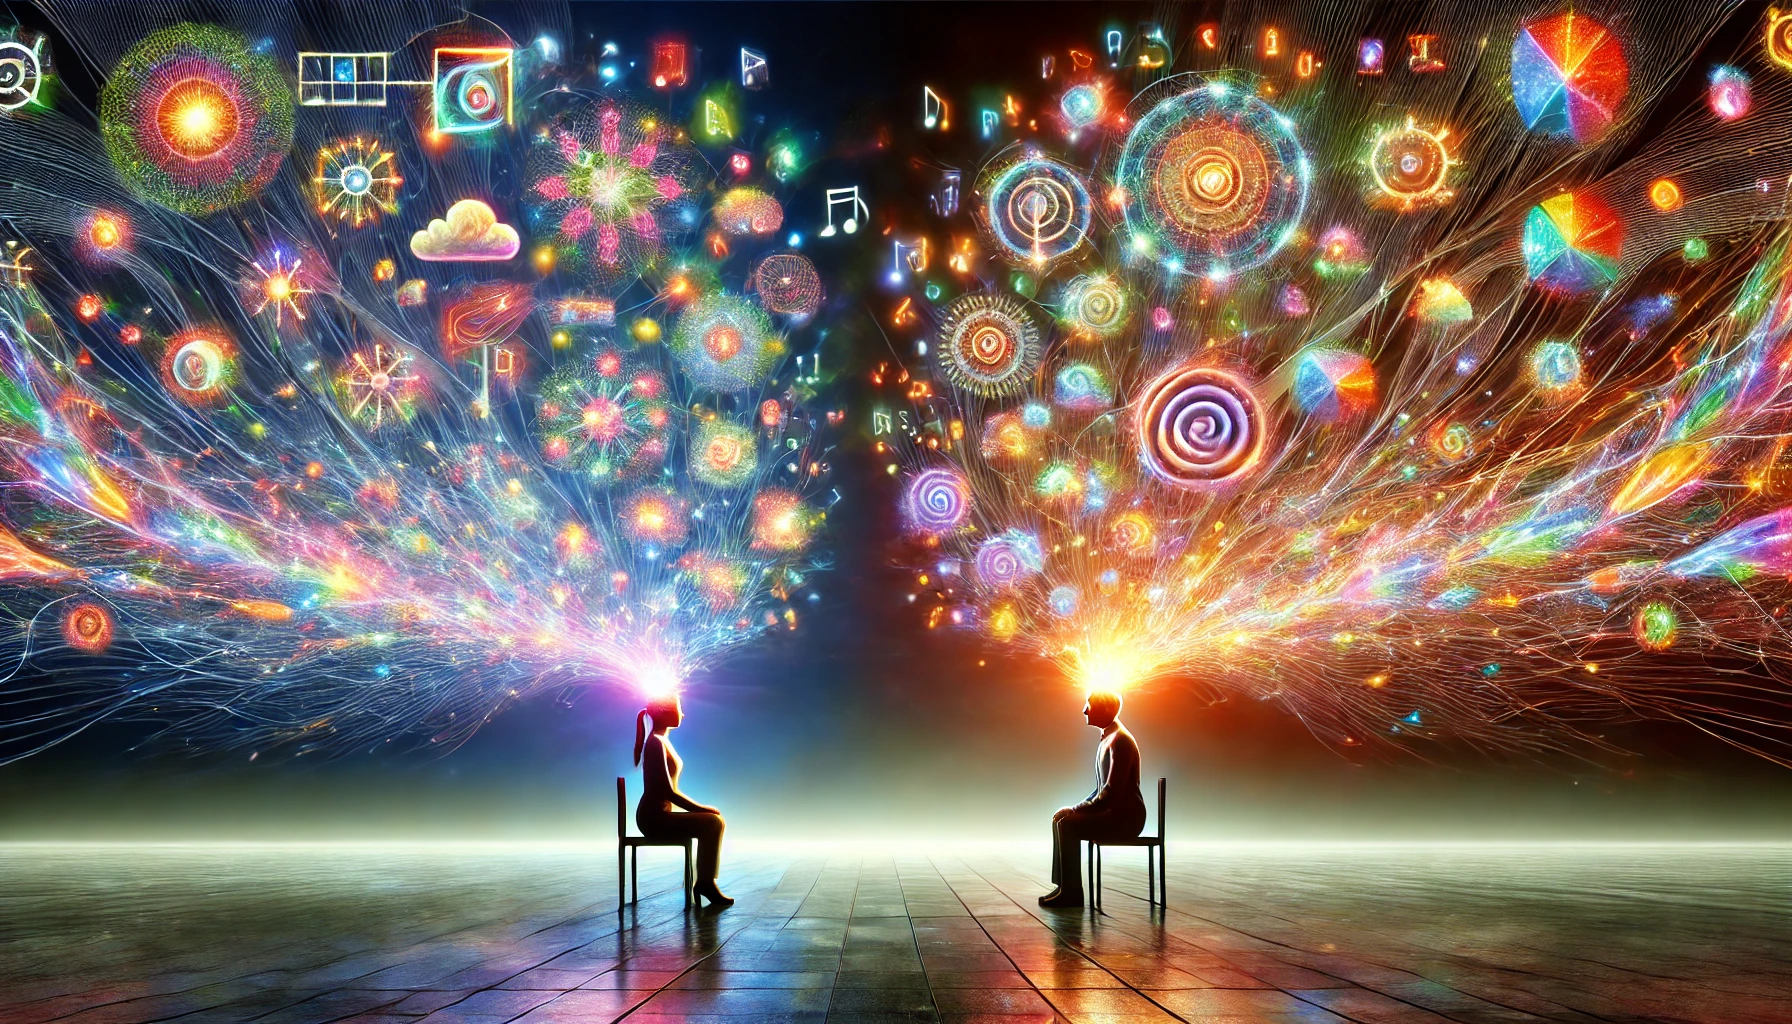
\includegraphics[width=0.8\textwidth]{language.png}

    \caption{Language as a form of telepathy}
\end{figure}

Research on conversational dynamics \cite{Enfield2017} reveals how consciousness achieves coherent states that enable real-time coordination between individuals. The sophisticated timing and turn-taking patterns in conversation demonstrate how consciousness maintains stable yet flexible patterns of organization that support fluid interpersonal communication while respecting physical constraints on information exchange.

The study of conceptual integration in language \cite{Fauconnier2002} illuminates how consciousness combines multiple domains of experience into unified linguistic expressions. This capacity for creative blending reveals how language enables sophisticated forms of conscious organization through specific patterns of energetic coherence that support both stability and innovation in communication.

Work on the origins of human communication \cite{Tomasello2008} suggests that language emerged from more basic forms of social coordination through increasingly sophisticated patterns of neural organization. This evolutionary perspective helps explain both the universal features of language and its unique capacity to support complex forms of conscious coordination between individuals.

Investigations of linguistic anthropology \cite{Silverstein1976} demonstrate how different societies achieve coherent communicative organization through distinct cultural frameworks. While language reflects shared biological foundations, its specific manifestations show how consciousness can maintain coherent states through various patterns of energetic organization shaped by cultural learning and social practice.

Recent theoretical syntheses \cite{Christiansen2016} suggest that language emerges from complex interactions between biological constraints, cognitive development, and cultural evolution. Rather than representing either pure biology or pure construction, language demonstrates how consciousness achieves coherent states through patterns of organization that integrate multiple levels of influence.

Research on brain-to-brain interfaces and linguistic communication \cite{Dingemanse2017} reveals how language enables precise coordination of conscious states across individuals while maintaining physical constraints on information transfer. This perspective helps explain both the remarkable effectiveness of linguistic communication and its inherent limitations.

The relationship between language and thought \cite{Whorf1956} gains new significance when examined through ECC's framework. Rather than simply reflecting or determining thought, language demonstrates how consciousness achieves coherent states through patterns of organization that enable both individual cognition and interpersonal communication.

The embodied nature of linguistic meaning \cite{Lakoff1999} takes on particular significance when examined through ECC's framework. Language works not through abstract symbol manipulation but through patterns of neural organization grounded in physical experience. This embodied foundation helps explain both the stability of linguistic meaning across individuals and the specific ways it can vary between cultures and contexts.

Research on gesture and thought \cite{McNeill2005} demonstrates how linguistic consciousness integrates multiple modalities into coherent communicative states. Rather than being mere supplements to speech, gestures reveal how consciousness achieves coherent expression through patterns of energetic organization that span both vocal and manual channels. This multimodal integration suggests fundamental principles about how consciousness maintains coherent states across different expressive systems.

Studies of language evolution \cite{Hauser2002} reveal how communicative systems emerge from specific patterns of neural organization that enable both individual thought and social coordination. This dual function helps explain why language exhibits both universal features reflecting shared biological constraints and tremendous variation reflecting cultural diversification.

The cultural scaffolding of linguistic consciousness \cite{Vygotsky2012} illuminates how communicative competence develops through structured social interaction. Language acquisition involves not just learning words and rules but developing sophisticated patterns of energetic coherence that enable participation in culturally specific forms of conscious coordination.

The role of language in distributing agency and coordinating social action \cite{Arbib2012} reveals how linguistic communication enables complex forms of collective organization. Through specific patterns of energetic coherence, language supports both individual consciousness and sophisticated forms of group coordination. This capacity for multi-level organization demonstrates how consciousness achieves states that serve both personal and collective functions.

Through this analysis, language emerges as a remarkable system for coordinating conscious states across individuals through specific patterns of energetic organization. Rather than representing arbitrary symbols or pure social construction, language demonstrates how consciousness achieves effective communication through sophisticated patterns of neural coherence that respect both biological constraints and cultural innovation. This understanding helps explain both language's universal features and its remarkable capacity for cultural elaboration.

The investigation of these linguistic principles suggests fundamental insights about consciousness itself - particularly how it maintains coherent states that enable both individual thought and social coordination through physically constrained patterns of energetic organization. This bridge between individual and collective consciousness through language represents one of the most sophisticated achievements of human neural organization.

\section{Math, Logic and Rationality}

Mathematical and logical thinking (i.e., symbolic reasoning) represent sophisticated achievements of conscious organization that require maintaining coherent states detached from immediate sensory experience. Recent work \cite{Lakoff2000} suggests that even abstract mathematical concepts emerge from embodied patterns of neural organization rather than purely symbolic manipulation. Through ECC's framework, mathematical cognition can be understood as requiring specific patterns of energetic coherence that support abstract relationships while remaining grounded in physical neural dynamics.

Research on the cognitive foundations of mathematics \cite{Dehaene2011b} reveals how numerical understanding emerges from basic patterns of neural organization that support quantity discrimination and spatial relationships. Rather than representing purely abstract symbols, mathematical concepts reflect sophisticated organizations of conscious experience that enable precise manipulation of quantitative relationships. This grounding helps explain both mathematics' power and its cognitive demands.

The anthropological study of mathematical practices \cite{Ascher1991} demonstrates how different cultures achieve coherent mathematical understanding through various patterns of organization. While certain aspects of mathematical thinking appear to reflect shared cognitive capacities, the specific ways that different societies develop mathematical concepts reveal how consciousness can achieve abstract coherence through culturally shaped patterns of energetic organization.

Work on the embodied basis of mathematical reasoning \cite{Lakoff2000} illuminates how abstract mathematical concepts emerge from patterns of neural activity grounded in sensorimotor experience. This perspective suggests that even highly abstract mathematics requires maintaining specific patterns of energetic coherence that remain connected to more basic forms of perceptual and motor organization.

The psychology of mathematical invention \cite{Hadamard1945} reveals how consciousness achieves novel mathematical insights through specific patterns of organization that enable creative recombination of existing concepts. This capacity for mathematical creativity demonstrates how consciousness can maintain coherent states that support both stability and innovation in abstract thinking.

Studies of mathematical cognition \cite{Devlin2000} suggest that mathematical ability emerges from coordinated activity across multiple neural systems rather than from an isolated "math module." This distributed organization reveals how consciousness achieves coherent mathematical states through patterns of energetic organization that integrate multiple processing streams while maintaining stable abstract relationships.

The relationship between mathematics and natural language \cite{MacLane1986} takes on new significance when examined through ECC's framework. Rather than representing a purely formal system, mathematics demonstrates how consciousness achieves coherent states through patterns of organization that enable both precise symbolic manipulation and communication of abstract concepts.

The development of mathematical intuition \cite{Penrose1994} reveals how consciousness achieves increasingly sophisticated patterns of abstract organization through experience. Rather than operating through purely formal rules, mathematical understanding emerges from specific patterns of energetic coherence that enable direct grasp of abstract relationships. This intuitive dimension demonstrates how consciousness maintains stable abstract states beyond simple symbol manipulation.

Research on mathematical discovery processes \cite{Lakatos1976} illuminates how new mathematical insights emerge through patterns of organization that combine logical rigor with creative exploration. The dynamic between proof and refutation demonstrates how consciousness achieves coherent mathematical states through patterns of energetic organization that enable both stability and innovation in abstract thinking.

Studies of mathematical enculturation \cite{Lloyd1990} reveal how different societies develop coherent systems of mathematical understanding through cultural practices. While mathematical truth may be universal, the specific ways that different cultures organize mathematical knowledge demonstrate how consciousness achieves abstract coherence through culturally shaped patterns of energetic organization.

Work on personal knowledge in mathematics \cite{Polanyi1958} suggests that mathematical understanding involves tacit dimensions that cannot be reduced to formal rules. This implicit aspect of mathematical knowledge reveals how consciousness maintains coherent abstract states through patterns of organization that extend beyond explicit symbolic representation.

The embodied mind perspective \cite{Varela1991} illuminates how mathematical cognition emerges from patterns of neural organization grounded in physical experience. Rather than representing purely abstract manipulation, mathematical thinking demonstrates how consciousness achieves coherent states through patterns of energetic organization that remain connected to embodied understanding.

Investigation of mathematical practices \cite{Rotman1993} reveals how consciousness maintains abstract coherence while enabling precise manipulation of mathematical relationships. The interplay between intuition and formalism demonstrates how consciousness achieves states that support both creative insight and rigorous proof through specific patterns of energetic organization.

Contemporary research on mathematical cognition \cite{DAmbrosio1985} suggests that mathematical ability emerges from coordinated activity across multiple neural systems. This distributed organization reveals how consciousness maintains coherent mathematical states through patterns of energetic coherence that integrate multiple processing streams.

Scientific understanding of rationality \cite{Gigerenzer2008} suggests that logical thinking emerges not from purely abstract rule-following but from sophisticated patterns of neural organization that enable reliable inference while respecting cognitive constraints. Through ECC's framework, rational thought can be understood as requiring specific patterns of energetic coherence that support abstract reasoning while remaining grounded in biological limitations.

The cultural transmission of mathematical knowledge \cite{Sperber1996} illuminates how abstract thinking develops through structured social interaction. Mathematical learning involves not just mastering formal systems but developing sophisticated patterns of energetic coherence that enable participation in culturally specific forms of abstract reasoning. This perspective helps explain both the universality of basic mathematical concepts and their diverse cultural elaborations.

Research on mathematical intuition \cite{Barrow1992} reveals how consciousness achieves direct grasp of abstract relationships through specific patterns of neural organization. Rather than operating solely through step-by-step deduction, mathematical understanding demonstrates how consciousness maintains coherent states that enable immediate recognition of mathematical truth while supporting rigorous verification.

The investigation of mathematical creativity \cite{Hadamard1945} demonstrates how consciousness generates novel insights through patterns of organization that enable flexible recombination of existing concepts. This creative dimension reveals how consciousness achieves states that support both stability and innovation in abstract thinking through specific patterns of energetic coherence.

Studies of mathematical development \cite{Piaget1952} show how abstract thinking emerges from more basic forms of cognitive organization. This developmental trajectory demonstrates how consciousness establishes increasingly sophisticated patterns of coherence that enable manipulation of abstract relationships while maintaining connection to embodied understanding.

From an ECC standpoint, logic and mathematical reasoning represent cognitively demanding processes precisely because they require the brain to maintain coherence in a domain that is largely "ungrounded" from typical energetic flows. In most conscious activities—such as perceiving the environment, processing emotions, or initiating motor responses—the underlying energetic patterns (electromagnetic fields, chemical gradients, and mechanical forces) correspond more or less directly to concrete features of the world. Logic and mathematics, however, compel the system to detach from these usual grounding points and instead uphold a set of abstract symbolic relationships, which the brain enacts by creating and sustaining new, internally consistent energetic configurations that do not map straightforwardly onto real-world inputs.

This detachment demands significant attentional resources and increased metabolic investment, as multiple brain networks must remain highly synchronized to support the manipulation of placeholders, free variables \footnote{In ECC, free variables are mental representations that can be manipulated independently of immediate physical grounding, enabling abstract thought while requiring active maintenance.}, or purely formal structures rather than intrinsic sensorimotor loops. This partly explains why symbolic reasoning is so effortful and resists parallelization (see \cite{Dehaene2011, kahneman2011thinking}); at least until a learned symbolic procedure can become more automatic.

In line with ECC, learning and engaging in mathematics or logic can be interpreted as a deliberate reorganization of energetic coherence at multiple hierarchical levels: the local fields in relevant cortical areas (prefrontal, parietal, and temporal regions), the global integrative dynamics that unify them, and possibly even transcriptomic or glial mechanisms that underlie adaptive neural plasticity. Early in the process of acquiring a new logical or mathematical skill, the mismatch between abstract reasoning and everyday bodily or perceptual coherence can be substantial, causing fatigue or frustration. Over time, with practice and repetition, certain neural patterns become more stable, reducing the energetic load required to manipulate purely formal concepts. Even so, these abstract tasks remain comparatively resource-intensive relative to more perceptually grounded actions, since sustaining abstract variables requires continuously preventing them from slipping back into more familiar, energetically efficient thought patterns.

Through this analysis, mathematical and logical thinking emerge as sophisticated achievements of conscious organization that require maintaining coherent states detached from immediate experience. Rather than representing purely formal manipulation, mathematical cognition demonstrates how consciousness achieves effective abstract thinking through specific patterns of neural coherence that respect both logical necessity and biological constraints. This understanding helps explain both mathematics' remarkable power and its significant cognitive demands.

The relationship between mathematical thinking and consciousness thus reveals fundamental principles about how neural systems achieve and maintain coherent states that support abstract reasoning while remaining grounded in physical reality. This balance between abstraction and embodiment represents one of the most sophisticated achievements of human conscious organization.

\section{Developmental Psychology and Neuroscience}

Through the lens of ECC, developmental psychology and neuroscience reveal fundamental principles about how conscious processing emerges through increasingly sophisticated patterns of energetic coherence. Recent theoretical work \cite{Bjorklund2014} suggests that cognitive development reflects not just maturation or learning but the progressive refinement of how neural systems maintain coherent conscious states. This developmental trajectory demonstrates how consciousness emerges through specific patterns of organization that become increasingly sophisticated over time.

Research on early brain development \cite{DehaeneLambertz2015} illuminates how neural systems establish basic patterns of coherent organization that support conscious processing. Rather than representing simple maturation, early development involves the careful coordination of multiple processes that create the conditions necessary for conscious experience. This foundation helps explain both the universal features of early development and its sensitivity to environmental input.

Studies of developmental psychopathology \cite{Cicchetti2016} demonstrate how disruptions to normal developmental processes can alter how consciousness achieves and maintains coherent states. These variations in developmental trajectories reveal how conscious organization depends on specific patterns of neural coherence that can be affected by both genetic and environmental factors.

The investigation of self-development \cite{Damasio2010} reveals how consciousness establishes increasingly sophisticated patterns of self-organization through experience. Rather than representing a simple accumulation of knowledge, the development of self-awareness demonstrates how consciousness achieves coherent states that integrate multiple aspects of experience into unified self-representation.

Work on neural plasticity and development \cite{Nelson2021} suggests that conscious capabilities emerge through specific patterns of neural organization that remain flexible throughout development. This plasticity reveals how consciousness maintains stable patterns of organization while enabling adaptation to environmental demands and learning opportunities.

Contemporary approaches to cognitive development \cite{Carey2009} demonstrate how children achieve increasingly sophisticated forms of conscious organization through structured interaction with their environment. This developmental progression reveals how consciousness establishes coherent states through patterns of energetic organization that become more refined through experience.

The relationship between brain development and consciousness \cite{Johnson2011} takes on new significance when examined through ECC's framework. Rather than simply supporting conscious processing, neural development creates the specific patterns of energetic coherence necessary for conscious experience.

Research on neural Darwinism \cite{Edelman1987} reveals how conscious capabilities emerge through selective stabilization of specific patterns of neural organization. This selective process demonstrates how consciousness achieves coherent states through patterns of energetic organization that prove adaptive for the developing organism while remaining flexible enough to incorporate new experiences.

Studies of probabilistic epigenesis \cite{Gottlieb2007} illuminate how conscious development emerges from complex interactions between genetic, neural, and environmental factors. Rather than following a predetermined program, conscious development demonstrates how coherent states emerge through bidirectional influences across multiple levels of organization.

The exploration of developmental motivation \cite{Kagan2013} reveals how consciousness maintains coherent states that guide behavior while enabling learning and adaptation. This motivational framework demonstrates how consciousness achieves states that support both stability and exploration through specific patterns of energetic organization.

Work on self and motivational systems \cite{Lichtenberg2016} suggests that conscious development involves the progressive refinement of how neural systems maintain coherent states that support both individual identity and social engagement. This dual development reveals how consciousness achieves increasingly sophisticated patterns of organization that serve both personal and interpersonal functions.

Research on the birth of mind \cite{Marcus2004} demonstrates how genetic factors shape the basic patterns of neural organization that support conscious processing. This biological foundation helps explain both the universal features of conscious development and the specific ways it can vary between individuals.

Contemporary approaches to psychoanalytic development \cite{Stern2000} reveal how consciousness establishes increasingly sophisticated patterns of emotional and interpersonal organization through early experience. This emotional development demonstrates how consciousness achieves coherent states that integrate affect, cognition, and social understanding.

Dynamic systems approaches \cite{Thelen1996} illuminate how conscious capabilities emerge from the coordinated activity of multiple developing systems. Rather than following a linear trajectory, conscious development demonstrates how coherent states emerge through complex interactions across multiple scales of organization.

The investigation of infant intersubjectivity \cite{Trevarthen2011} reveals how consciousness achieves coherent states that enable social coordination from the earliest stages of development. This early social capacity demonstrates how consciousness maintains patterns of organization that support both individual experience and interpersonal engagement through specific forms of energetic coherence.

Research on interpersonal neurobiology \cite{Siegel2020} illuminates how conscious development emerges through the interaction between neural maturation and social relationships. Rather than representing purely individual processes, conscious development demonstrates how coherent states emerge through patterns of organization shaped by both biological constraints and interpersonal experience.

Studies of the unconscious mind's development \cite{Schore2019} suggest that conscious organization involves multiple levels of processing that become increasingly integrated through development. This multi-level integration reveals how consciousness achieves coherent states through patterns of energetic organization that span both explicit and implicit processing.

The investigation of neural development \cite{Quartz2002} demonstrates how conscious capabilities emerge through specific patterns of neural organization that remain plastic throughout life. This ongoing plasticity reveals how consciousness maintains stable patterns of organization while enabling continued adaptation and learning across the lifespan.

Through this analysis, developmental psychology and neuroscience illuminate fundamental principles about how consciousness emerges from and maintains coherent states through specific patterns of neural organization. Rather than representing either pure maturation or pure construction, conscious development demonstrates how effective organization emerges through sophisticated patterns of energetic coherence that respect both biological constraints and environmental influence.

This developmental perspective suggests that consciousness requires specific trajectories of neural organization to establish and maintain coherent states. This understanding has profound implications for both theoretical models of consciousness and practical approaches to supporting healthy development. It suggests that conscious experience emerges through carefully orchestrated patterns of development that enable increasingly sophisticated forms of coherent organization while maintaining fundamental stability.

The relationship between development and consciousness thus reveals essential principles about how neural systems achieve and maintain coherent states that support adaptive functioning while enabling ongoing learning and growth. This balance between stability and plasticity represents one of the most remarkable achievements of biological organization.

\section{Free Will and Agency}

Through ECC's framework, free will and agency emerge from conscious systems' capacity to maintain and modify coherent states through specific patterns of energetic organization. Recent theoretical work \cite{Deacon2011} suggests that agency arises not from abstract decision-making processes but from organisms' ability to generate and select among possible actions through coherent patterns of neural activity. This perspective aligns with evidence demonstrating how voluntary action emerges from sophisticated patterns of biological organization.

Research on the neuroscience of volition \cite{Clark2001} reveals how voluntary actions emerge from coordinated activity across multiple neural systems rather than from a centralized "decision center." Through ECC's framework, free will can be understood as the lived experience of being the process that enacts change through coherent energy flows, rather than as an abstract capacity for uncaused causation.

Studies of intentional behavior \cite{Juarrero1999} demonstrate how agency emerges from complex systems capable of self-organization and recursive feedback. Rather than requiring freedom from causation, genuine agency reflects organisms' capacity to maintain coherent states that enable both stability and adaptive response through specific patterns of energetic organization.

Contemporary approaches to free will \cite{Dennett2003} illuminate how voluntary action emerges from sophisticated biological mechanisms that enable both reliable behavior and flexible adaptation. This perspective suggests that free will reflects consciousness's capacity to maintain coherent states that support both determined and innovative actions through specific patterns of neural organization.

Work on top-down causation \cite{Ellis2016} reveals how conscious systems achieve coherent states that enable genuine agency while respecting physical constraints. Rather than violating causation, free will emerges from consciousness's capacity to maintain patterns of energetic coherence that support both reliable function and meaningful choice.

The investigation of effective intentions \cite{Mele2009} demonstrates how consciousness achieves states that enable both planned action and spontaneous response through specific patterns of organization. This dual capacity reveals how consciousness maintains coherent states that support both deliberate and immediate agency through sophisticated patterns of energetic coherence.

Research on embodied cognition \cite{Noe2009} suggests that agency emerges from organisms' active engagement with their environment rather than from abstract computation. This perspective aligns with ECC's emphasis on how consciousness achieves coherent states through patterns of organization that remain grounded in physical reality.

Research on dynamical systems approaches to agency \cite{Thompson2007} reveals how conscious systems maintain coherent states that enable both stability and flexibility in action. Rather than requiring freedom from causation, genuine agency emerges from consciousness's capacity to achieve patterns of energetic organization that support both reliable behavior and adaptive response.

Studies of personal causation \cite{OConnor2000} demonstrate how consciousness achieves coherent states that enable genuine self-directed action while respecting physical constraints. This perspective suggests that free will emerges not from uncaused causation but from specific patterns of neural organization that support both determined and innovative behavior.

The investigation of natural autonomy \cite{Walter2001} illuminates how conscious systems achieve coherent states that enable meaningful choice without requiring libertarian free will. Through ECC's framework, agency can be understood as emerging from consciousness's capacity to maintain patterns of energetic coherence that support genuine self-direction while remaining grounded in physical causation.

Work on the significance of free will \cite{Kane1996} reveals how consciousness maintains coherent states that enable both moral responsibility and innovative action. Rather than requiring absolute freedom, genuine agency emerges from consciousness's capacity to achieve patterns of organization that support both reliable function and meaningful choice.

Contemporary research on biological autonomy \cite{Kauffman2000} suggests that agency emerges from living systems' capacity to maintain coherent organization while enabling adaptive response. This perspective aligns with ECC's emphasis on how consciousness achieves states that support both stability and flexibility through specific patterns of energetic coherence.

Studies of dynamic patterns in behavior \cite{Kelso1995} demonstrate how conscious systems maintain coherent states that enable coordinated action across multiple timescales. This temporal organization reveals how consciousness achieves patterns of energetic coherence that support both immediate response and extended planning.

The relationship between will and personhood \cite{Frankfurt1971} takes on new significance when examined through ECC's framework. Rather than requiring libertarian free will, genuine agency emerges from consciousness's capacity to maintain coherent states that enable both self-reflection and effective action.

Research on the emergence of agency in biological systems \cite{Barandiaran2009} reveals how consciousness achieves coherent states that enable meaningful self-direction while respecting physical constraints. This biological foundation demonstrates how free will emerges from specific patterns of neural organization rather than requiring freedom from causation.

Studies of individual agency and normativity \cite{Taylor1985} illuminate how consciousness maintains coherent states that enable both reliable behavior and genuine innovation. Through patterns of energetic organization that support both stability and flexibility, conscious systems achieve forms of agency that transcend simple determinism while remaining grounded in physical reality.

The investigation of agency in social contexts \cite{Bandura2001} demonstrates how consciousness achieves coherent states that enable both individual action and social coordination. Rather than existing in isolation, agency emerges through patterns of organization that support both personal autonomy and effective social interaction.

Work on investigations of autonomous systems \cite{Kauffman2000} reveals how agency emerges from living systems' capacity to maintain coherent organization while enabling adaptive response. This biological autonomy demonstrates how consciousness achieves states that support both stability and flexibility through specific patterns of energetic organization.

Through this analysis, free will and agency emerge as sophisticated achievements of conscious organization rather than metaphysical mysteries. Rather than requiring freedom from causation, genuine agency demonstrates how consciousness maintains coherent states through patterns of energetic organization that enable both reliable function and meaningful choice.

The framework suggests that free will, while constrained by physical laws, reflects consciousness's capacity to maintain and modify coherent states through sophisticated patterns of neural organization. This understanding helps resolve traditional debates about free will by grounding agency in actual biological capabilities while preserving the reality of meaningful choice and self-direction.

The relationship between agency and consciousness thus reveals fundamental principles about how neural systems achieve and maintain coherent states that support both determined and innovative behavior. This balance between reliability and flexibility represents one of the most sophisticated achievements of conscious organization in biological systems.

\newpage
\section{References}
\printbibliography[title={},heading=subbibliography]
%\printbibliography[title={References: Biological and Psychological Implications}]
\end{refsection}

\section*{\phantom{Part VII Anthropological Implications}}
\h{A New Anthropology}

\begin{refsection}[references/0001_8_new_anthro.bib]

\section{Foundations}

The framework of Energetically Coherent Computation suggests a fundamental reconceptualization of anthropological theory. Where traditional approaches have often struggled to bridge the divide between biological and cultural analysis, ECC offers a way to understand human social and cultural life as emerging from patterns of energetic coherence that span multiple scales of organization, from cellular dynamics to collective social fields.

This new anthropology begins not with the traditional opposition between nature and culture, but with understanding how meaning emerges from physically grounded patterns of energetic coherence. Unlike computational approaches that treat meaning as abstract symbol manipulation, or purely interpretive approaches that disconnect meaning from physical reality, ECC suggests how cultural meanings arise from and remain grounded in specific patterns of energy organization within biological systems.

The physical grounding of cultural meaning through ECC resolves several persistent challenges in anthropological theory. First, it addresses the symbol grounding problem by showing how meanings emerge from physically indexed states rather than floating free in abstract semantic space. Cultural symbols work not through arbitrary convention alone, but through their capacity to establish and maintain specific patterns of energetic coherence across individuals and groups.

Second, this approach illuminates how shared cultural understandings become possible. Rather than positing abstract cultural templates or reducing culture to neural firing patterns, ECC suggests how cultural knowledge emerges from aligned patterns of energetic coherence maintained through ongoing social practice. This explains both the stability of cultural forms and their capacity for transformation through time.

Third, ECC provides a framework for understanding embodied knowledge and skill. Instead of separating cultural knowledge from bodily practice, the framework shows how knowledge inherently involves developing and maintaining specific patterns of energetic coherence through physical engagement with the world. This helps explain why cultural transmission often requires direct bodily practice rather than just verbal instruction.

Most significantly, this new anthropology transcends traditional divisions between materialist and interpretive approaches. By grounding meaning in patterns of energetic coherence while acknowledging the irreducibility of conscious experience, ECC suggests how cultural analysis can be simultaneously materialist in its foundations and interpretive in its methods.

\subsection{Physical Grounding of Cultural Meaning}

The physical grounding of cultural meaning has presented a persistent challenge for anthropological theory. While materialist approaches risk reducing meaning to neural activity, interpretive approaches often leave unclear how meanings maintain stability across time and space \cite{dandrade1995development}. Energetically Coherent Computation (ECC) offers a novel resolution by demonstrating how cultural meanings emerge from and are maintained by specific patterns of energetic coherence in biological systems.

At its most fundamental level, meaning arises from the brain's capacity to maintain stable patterns of energetic coherence that integrate sensory experience, emotional resonance, and social understanding. These patterns are not arbitrary but are constrained by cellular architecture and transcriptomic profiles that create what ECC terms a "rich alphabet" of possible states. This biological grounding explains both why certain meaningful patterns recur across cultures and why cultural elaboration can take such diverse forms \cite{bloch2012anthropology}.

Unlike traditional symbol systems theory \cite{harnad1990symbol}, which treats meanings as arbitrary cultural conventions, ECC suggests that symbols work by establishing and maintaining specific patterns of energetic coherence across individuals. When members of a culture encounter meaningful objects, practices, or words, these stimuli trigger coherent patterns of neural activity that have been shaped through sustained cultural practice. These patterns remain physically grounded while enabling abstract thought and complex cultural understanding \cite{lakoff1999philosophy}.

The framework particularly illuminates how ritual objects and practices acquire and maintain their power \cite{bell1992ritual}. Rather than serving as mere carriers of abstract meaning, ritual elements help establish and maintain specific patterns of energetic coherence across participants. This explains both why certain material forms prove especially effective in ritual contexts and why ritual meaning cannot be reduced to verbal explanation alone \cite{turner1967forest}.

Similarly, ECC suggests how sacred spaces and objects maintain their significance through time. Places and things that reliably evoke particular patterns of energetic coherence become recognized as inherently meaningful or powerful. This grounding in physical dynamics explains both the stability of sacred meanings and their resistance to purely rational analysis \cite{eliade1959sacred}. The framework suggests how objects and spaces can accumulate meaning through their capacity to establish and maintain patterns of coherence across generations of cultural practice \cite{keane2003semiotics}.

This physical grounding of meaning does not reduce cultural significance to neural activity but rather shows how meaning necessarily emerges from and remains connected to patterns of energetic coherence. The framework suggests new approaches to studying how meanings are established, maintained, and transformed through ongoing social practice while remaining anchored in physical reality \cite{csordas1990embodiment}.

The relationship between stability and variation in cultural meanings takes on new significance when examined through ECC's framework. Consider how certain symbols and practices maintain remarkable stability across generations while others prove highly mutable \cite{sperber1996explaining}. Through ECC, we can understand this as reflecting different degrees of constraint in the underlying patterns of energetic coherence. Some meaningful configurations, particularly those tied to basic emotional and social experiences, find ready anchoring in human neural architecture. Others, more dependent on specific cultural elaboration, require constant social reinforcement to maintain stability \cite{boyer1994naturalness}.

This perspective illuminates foundational insights about techniques of the body \cite{bourdieu1990logic}. Where earlier work observed how basic human activities like walking or swimming take culturally specific forms, ECC suggests how these patterns become stabilized through specific configurations of energetic coherence. The framework explains both why certain bodily techniques prove easily transmissible across cultures and why others remain stubbornly resistant to change \cite{ingold2000perception}.

The maintenance of coherent meaning systems requires continuous energetic work at both individual and collective levels. Ritual practices, formal education, and everyday social interaction all serve to establish and reinforce particular patterns of coherence across social groups \cite{hutchins1995cognition}. This explains why cultural transmission typically requires extended periods of immersion and practice rather than simple instruction. New members of a culture must develop specific patterns of energetic coherence through direct engagement rather than merely learning abstract rules or symbols \cite{tomasello1999cultural}.

These insights have particular relevance for understanding traditional knowledge systems. Rather than treating such knowledge as either purely practical or purely symbolic, ECC suggests how sophisticated understanding can emerge from and remain grounded in patterns of energetic coherence while enabling abstract thought and complex cultural elaboration \cite{varela1991embodied}. This helps explain why traditional knowledge, such as ecological understanding or healing practices, often proves more sophisticated than initially apparent to outside observers \cite{jackson1996things}.

The framework offers novel insight into how different societies can maintain radically different but equally valid systems of meaning while sharing basic human neural architecture \cite{merleau1962phenomenology}. The rich alphabet of possible coherent states enabled by human biology allows for tremendous cultural variation while imposing certain universal constraints. This explains why certain basic patterns of meaning-making appear across cultures while taking culturally specific forms \cite{throop2003articulating}.

The implications for understanding classification systems and knowledge organization are particularly significant. Traditional approaches to classification, as documented in ethnographic research, demonstrate how societies develop sophisticated systems for organizing knowledge that integrate sensory experience, practical utility, and cultural meaning \cite{ellen2016cultural}. Through ECC, these classification systems can be understood not as arbitrary cultural constructions but as emergent patterns of coherence that enable effective engagement with both physical and social worlds \cite{levi1966savage}.

This understanding has profound implications for how we conceptualize power relations in knowledge systems. The ability to shape and maintain particular patterns of coherence represents a fundamental form of social power \cite{foucault1980power}. However, unlike purely constructivist approaches that risk reducing knowledge to power relations alone, ECC demonstrates how knowledge systems must maintain effective engagement with physical reality while serving social functions \cite{scott1998seeing}.

The framework also provides new perspective on how scientific and traditional knowledge systems relate to each other. Rather than positioning these as opposing ways of knowing, ECC suggests how different knowledge traditions represent distinct but potentially complementary patterns of coherence for understanding reality \cite{latour1999pandora}. This helps explain both why certain forms of knowledge prove especially effective in particular contexts and how different knowledge systems might productively inform each other.

Understanding meaning through patterns of energetic coherence ultimately suggests new approaches to both theoretical analysis and practical engagement with cultural systems. By grounding meaning in physical dynamics while acknowledging the genuine creativity of cultural elaboration, ECC offers ways to move beyond traditional debates about relativism versus universalism in anthropological theory \cite{wolf1999envisioning}. This framework provides tools for understanding both the remarkable diversity of human cultural systems and their foundation in shared biological capacities for maintaining coherent patterns of meaning.


\subsection{The Symbol Grounding Problem Reconsidered}

The symbol grounding problem manifests in both cognitive science and semiotics as the challenge of infinite regression in meaning. The fundamental question of how abstract symbols acquire meaning cannot be resolved through purely computational or formal approaches \cite{harnad1990symbol}. This parallel recognition across disciplines suggests something fundamental about the nature of meaning that ECC's framework helps illuminate.

Traditional anthropological approaches have demonstrated how symbols operate within cultural systems primarily through their relationships to other symbols \cite{saussure1983course}. However, if meaning emerges solely from differential relations between signs, we face a fundamental paradox: how does the system as a whole acquire its grip on reality? ECC suggests a resolution by showing how symbolic systems remain anchored in patterns of energetic coherence while enabling complex chains of reference.

This grounding occurs not through simple one-to-one correspondence between symbols and physical states, but through the maintenance of coherent energy patterns that integrate multiple levels of experience \cite{lakoff1999philosophy}. A symbol's meaning emerges from its capacity to establish and maintain specific configurations of energetic coherence across individuals while enabling connection to other symbols. This explains both how symbols can participate in endless chains of reference while maintaining meaningful connection to physical reality \cite{peirce1931collected}.

The framework particularly illuminates how symbols maintain stability across time and social space. Rather than treating symbolic meaning as either purely conventional or naturally determined, ECC suggests how meanings emerge from sustained patterns of practice that establish specific forms of neural coherence \cite{barsalou1999perceptual}. This helps explain both the remarkable stability of certain symbolic forms across generations and their capacity for transformation through changes in practice.

Through ECC's framework, we can understand how symbolic systems acquire meaning not through arbitrary cultural assignment but through their capacity to establish and maintain specific patterns of energetic coherence that integrate sensory, emotional, and cognitive dimensions of experience \cite{varela1991embodied}. This perspective helps resolve long-standing debates about symbolic meaning while suggesting new approaches to understanding how symbols actually work in human cultural systems.

This resolution of infinite semiotic chains through energetic coherence resonates with multiple theoretical frameworks across disciplines. The conception of scientific knowledge as a vast web of interconnected beliefs, extending from the periphery of empirical observation to central theoretical commitments, finds natural expression through ECC \cite{quine1960word}. Rather than requiring absolute foundations, beliefs maintain their coherence through mutual support while remaining anchored in patterns of energetic organization that connect them to physical reality.

The co-evolution of symbolic capacity and neural organization takes on new significance through this lens \cite{deacon1997symbolic}. Rather than treating symbols as either purely biological or cultural phenomena, ECC suggests how symbolic systems emerge from and remain grounded in specific patterns of neural organization while enabling sophisticated cultural elaboration. This explains both the universal aspects of human symbolic capacity and its tremendous cultural variability.

Understanding symbols through patterns of energetic coherence helps resolve traditional debates about meaning and reference. Rather than choosing between referential and differential theories of meaning, ECC suggests how symbols work by establishing patterns of coherence that enable both stable reference and complex interrelation \cite{searle1980minds}. This perspective helps explain both how symbols maintain reliable connection to physical reality and how they participate in elaborate cultural systems.

The embodied nature of symbolic meaning gains particular clarity through this framework \cite{hutchins1995cognition}. Symbols do not operate through abstract computation but through their capacity to establish and maintain specific patterns of energetic coherence grounded in sensorimotor experience. This embodied grounding explains both why certain symbolic forms prove especially effective and how abstract thought remains connected to physical experience.

These theoretical perspectives align with contemporary understanding of embedding spaces in machine learning and cognitive neuroscience. Just as neural networks create high-dimensional spaces where similar concepts cluster together, human neural architecture enables the emergence of meaningful patterns through its capacity to maintain specific configurations of energetic coherence. However, unlike artificial embedding spaces, these biological embeddings remain directly connected to physical reality through their grounding in cellular dynamics and embodied experience \cite{lakoff1999philosophy}.

The key distinction is that biological embedding spaces are not arbitrary projections but emerge from and remain constrained by patterns of energetic coherence shaped by both neural architecture and cultural practice \cite{varela1991embodied}. This explains why certain conceptual relationships prove remarkably stable across cultures while others show tremendous variation. The framework suggests how abstract thought can extend through endless chains of reference while maintaining meaningful connection to physical reality through its foundation in coherent energy dynamics.

Understanding symbols as patterns of energetic coherence within biological embedding spaces also illuminates how novel meanings can emerge through recombination and metaphorical extension \cite{lakoff1999philosophy}. Just as neural networks can discover new relationships through exploration of their embedding spaces, human consciousness can establish new patterns of coherence that integrate multiple domains of experience while remaining grounded in physical reality.

The framework particularly helps resolve persistent questions about symbolic abstraction and creative innovation. Rather than seeing abstract thought as detached from physical reality, ECC suggests how sophisticated conceptual systems emerge from and remain grounded in patterns of energetic coherence \cite{barsalou1999perceptual}. This explains both how symbols enable abstract reasoning and why such reasoning remains constrained by embodied experience.

The social dimension of symbol grounding takes on new significance through this perspective \cite{hutchins1995cognition}. Symbols acquire and maintain their meaning not through individual mental operations alone but through patterns of coherence established and maintained through collective practice. This social grounding helps explain both why symbolic systems require cultural transmission and how they enable coordination across social groups.

This reconceptualization of the symbol grounding problem through ECC suggests new approaches to understanding both human cognition and artificial intelligence. Rather than attempting to ground symbols through purely computational means, the framework indicates how meaningful symbolic systems must emerge from and remain connected to patterns of energetic coherence that integrate multiple dimensions of experience \cite{harnad1990symbol}. This understanding has profound implications for both cognitive science and the development of artificial systems capable of genuine symbolic understanding.

\subsection{Rich Alphabets and Cultural Representation}

The concept of rich alphabets, central to ECC's framework, provides a crucial bridge between biological capacity and cultural elaboration. Unlike computational systems that operate through binary states or artificial neural networks limited by their architecture, human neural systems maintain vast repertoires of possible coherent states shaped by transcriptomic profiles and cellular organization. This biological foundation enables the remarkable sophistication of human cultural representation while explaining certain universal constraints on cultural forms \cite{shore1996culture}.

Where traditional anthropology has often struggled to explain how cultures can be simultaneously diverse and constrained, the rich alphabet concept suggests how tremendous variation can emerge from common biological foundations. Each culture elaborates distinct patterns of meaning from the vast space of possible coherent states enabled by human neural architecture. Yet these elaborations must work within constraints imposed by the physical requirements of maintaining energetic coherence \cite{wagner1981invention}.

The framework particularly illuminates how different societies develop sophisticated systems of cultural representation that integrate multiple dimensions of experience. Rather than treating cultural knowledge as either purely symbolic or purely practical, ECC suggests how complex understanding emerges from patterns of coherence that span sensory, emotional, and conceptual domains \cite{geertz1973interpretation}. This helps explain both the remarkable stability of certain cultural forms and their capacity for endless innovation.

This perspective proves especially valuable for understanding what structural anthropology identified as universal patterns in human thought \cite{levistrauss1963structural}. Rather than seeing these patterns as abstract logical structures, ECC suggests how they emerge from fundamental properties of how neural systems maintain coherent states. The binary oppositions and transformational relationships identified by structuralism reflect stable configurations that neural systems can reliably maintain and transmit across generations.

The rich alphabet concept provides new insight into how societies develop and maintain systems of meaning that transcend individual experience while remaining grounded in shared biological capacities \cite{rappaport1999ritual}. Different cultures elaborate distinct but equally sophisticated patterns of coherence that enable both individual expression and collective coordination. This explains both the universal aspects of cultural representation and its tremendous diversity across human societies.

The interaction between biological constraints and cultural elaboration gains particular clarity through the rich alphabet framework \cite{descola2013beyond}. While certain patterns of neural organization create natural fault lines that shape cultural possibilities, the vast space of possible coherent states enables tremendous creativity in how societies organize experience and meaning. This helps explain both why certain cultural forms recur across societies and why radical innovation remains possible.

The remarkable sophistication of what have been termed "archaic" thought systems takes on new significance through this lens \cite{turner1967forest}. Rather than representing primitive precursors to modern rationality, such systems demonstrate how societies can develop complex patterns of coherence that integrate multiple dimensions of experience. These systems often achieve forms of understanding inaccessible to purely analytical approaches while maintaining their own rigorous forms of coherence.

This perspective particularly illuminates the relationship between conscious experience and cultural representation \cite{jung1968archetypes}. Different societies develop distinct but equally valid patterns of coherence for organizing conscious states, leading to what might be called cultural modes of consciousness. These patterns reflect neither pure biological determinism nor arbitrary cultural construction but emerge from the interaction between neural architecture and sustained cultural practice.

The framework helps explain why certain symbolic forms prove especially powerful or persistent across cultures \cite{armstrong1981powers}. Elements that engage multiple dimensions of neural organization - integrating sensory, emotional, and conceptual patterns of coherence - tend to maintain greater stability and transmissibility. This explains the enduring power of certain religious symbols, artistic forms, and narrative structures while allowing for tremendous cultural variation in their specific manifestations.

Through the rich alphabet framework, we can better understand how sophisticated cultural knowledge becomes established and transmitted across generations \cite{whitehouse2004modes}. Rather than requiring either pure memorization or abstract understanding, cultural transmission involves developing specific patterns of coherence through sustained practice and engagement. This explains why certain forms of knowledge prove especially resistant to verbal explanation while remaining reliably transmissible through direct participation.

The framework provides particular insight into how different societies maintain distinct but equally sophisticated systems of representation while sharing common neural architecture \cite{bateson1972steps}. Rather than treating cultural differences as either surface variations or incommensurable worldviews, ECC suggests how diverse patterns of coherence can emerge from shared biological foundations. This helps resolve long-standing debates about universality and relativism in anthropological theory.

The relationship between individual experience and collective representation becomes clearer through this perspective. While each person develops unique patterns of coherence through their particular history, cultural systems provide frameworks that enable shared understanding and coordination \cite{shore1996culture}. This explains both how cultural knowledge transcends individual experience and how it remains grounded in embodied understanding.

The rich alphabet concept also illuminates how societies maintain complex systems of knowledge that integrate practical, emotional, and cosmic dimensions of experience \cite{wagner1981invention}. Rather than separating these domains as modern thought often does, many traditional systems achieve sophisticated integration through patterns of coherence that span multiple levels of reality. This helps explain both their practical effectiveness and their resistance to reduction to purely technical knowledge.

The implications extend beyond theoretical understanding to practical engagement with cultural systems. By recognizing how meaning emerges from patterns of energetic coherence rather than arbitrary convention, we can better appreciate both the flexibility and constraints of cultural innovation \cite{rappaport1999ritual}. This suggests new approaches to cultural preservation and transformation that respect both biological foundations and cultural creativity.

These insights prove particularly valuable for understanding contemporary global challenges. As societies navigate unprecedented technological and environmental changes, the rich alphabet framework suggests how new patterns of coherence might emerge that integrate traditional wisdom with contemporary understanding \cite{bateson1972steps}. This offers hope for developing more sophisticated approaches to cultural adaptation while maintaining connection to established patterns of meaning and practice.

\subsection{Neural Light Cones and Social Experience}

The concept of neural light cones, introduced in ECC's physical framework, provides unexpected insight into fundamental questions of social anthropology. Just as conscious integration cannot exceed certain spatial and temporal boundaries determined by patterns of energetic propagation, social experience operates within similar constraints that shape how meaning and influence can spread through social fields. This perspective offers new ways to understand both the limitations and the remarkable achievements of human social coordination \cite{durkheim1995elementary}.

Where classic social theory has struggled to explain how individual consciousness relates to collective representations, neural light cones suggest how patterns of coherence can propagate across social groups while maintaining physical constraints \cite{schutz1967phenomenology}. The social fact - that collective phenomena exercise genuine causal force on individuals - can be understood through how patterns of energetic coherence establish stable fields that shape individual experience and action while remaining grounded in physical dynamics.

Consider how ritual creates temporary zones of heightened social coordination through careful manipulation of attention, movement, and emotional arousal. These practices effectively (not literally) expand the neural light cones of participants, enabling broader patterns of coherence than normally possible in everyday social interaction \cite{turner1969ritual}. This explains both the power of ritual to create experiences of collective effervescence and its inherent temporal limitations - such states cannot be maintained indefinitely due to fundamental constraints on energetic coherence.

Techniques of the body represent reliable ways of establishing specific patterns of energetic coherence that can be transmitted across generations \cite{mauss1973techniques}. The neural light cone concept helps explain why certain techniques prove easily transmissible while others require extensive practice to master - they represent different degrees of complexity in establishing and maintaining coherent states.

This perspective also offers new insight into the anthropological observation that social influence typically operates through direct personal interaction rather than abstract rules or principles \cite{goffman1967interaction}. The constraints of neural light cones suggest why face-to-face interaction proves especially effective in transmitting and maintaining cultural patterns - it enables direct alignment of energetic coherence between individuals through multiple sensory and emotional channels.

This framework helps explain why certain scales of social organization prove particularly stable or challenging across cultures. Small groups operating within the bounds of direct personal interaction - families, work teams, ritual congregations - represent scales at which humans can naturally maintain coherent states that align \cite{hutchins1995cognition}. Larger social formations require sophisticated cultural technologies to extend coordination beyond these natural limits, explaining why institutions, hierarchies, and symbolic systems take remarkably similar forms across societies despite surface variations.

The temporal aspects of neural light cones prove especially revealing for understanding social rhythms. Just as conscious integration operates within specific temporal windows, social coordination requires careful management of timing across multiple scales \cite{mcneill1995keeping}. Ritual calendars, work schedules, and life cycle ceremonies can be understood as technologies for extending social coherence beyond immediate temporal bounds while respecting fundamental constraints on human attention and energy.

Consider how different societies manage the challenge of maintaining coherence across spatial and temporal distances. Writing systems, monuments, and traditional oral practices represent different solutions to extending patterns of energetic coherence beyond immediate face-to-face interaction \cite{thompson2001radical}. The effectiveness of these technologies depends on their ability to reliably evoke and maintain specific patterns of coherence across individuals and generations while working within neural light cone constraints.

The framework also illuminates power relations in new ways. Those who can effectively manipulate conditions for establishing and maintaining coherent states across social groups - through ritual expertise, rhetorical skill, or institutional authority - exercise genuine influence over collective experience and action \cite{bourdieu1977outline}. This suggests why certain forms of authority prove remarkably stable across cultures while others require constant reinforcement through displays of force or symbolic power.

The concept of embodied knowledge gains particular clarity through this lens \cite{csordas1994embodiment}. Rather than treating bodily knowledge as either pure technique or cultural symbolism, we can understand how specific patterns of energetic coherence emerge from and remain grounded in physical practice while enabling cultural elaboration. This explains both the stability of embodied knowledge across generations and its resistance to verbal explanation or formal codification.

The study of intersubjective experience takes on new significance through this framework \cite{merleau2012phenomenology}. Rather than treating shared understanding as either mysterious resonance or purely cognitive modeling, neural light cones suggest how patterns of coherence are bridged across individuals through embodied interaction and shared attention. This explains both the immediacy of intersubjective understanding and its dependence on specific conditions of social engagement.

The phenomenological emphasis on the lived body finds natural extension through neural light cones \cite{jackson1989paths}. The framework suggests how bodily experience creates natural boundaries and possibilities for social coherence, explaining both why certain forms of social coordination prove especially stable and how they can be extended through cultural technologies. This helps resolve traditional tensions between phenomenological and social structural approaches to understanding human experience.

These insights have particular relevance for understanding contemporary transformations in social experience through digital technologies \cite{thompson2001radical}. Rather than seeing virtual interaction as either pure simulation or genuine social presence, the framework suggests how different technologies create distinct conditions for establishing and maintaining patterns of coherence across individuals. This explains both the possibilities and limitations of technologically mediated social interaction.

The implications extend beyond theoretical understanding to practical approaches for fostering social coordination and cultural transmission. By recognizing how patterns of coherence operate within specific spatial and temporal constraints, we can better appreciate both the remarkable achievements of traditional social technologies and the challenges facing contemporary attempts to maintain coherence across increasingly distributed social networks \cite{hutchins1995cognition}.

Through careful attention to how neural light cones shape the possibilities for social experience, we gain deeper insight into both the universal aspects of human sociality and the tremendous diversity of cultural solutions for extending coherence beyond immediate spatial and temporal bounds. This framework suggests new approaches to understanding both traditional social forms and emerging patterns of human coordination in our increasingly connected world.


\section{Theoretical Frameworks}

Having established how ECC provides new foundations for anthropological understanding through physically grounded patterns of energetic coherence, we can now reexamine major theoretical frameworks in anthropology through this lens. Rather than treating these frameworks as competing explanations, ECC suggests how different theoretical approaches have captured distinct aspects of how human consciousness and culture emerge from patterns of energetic organization.

Structuralism's emphasis on binary opposition and transformational logic, for instance, reflects fundamental properties of how neural systems maintain stable patterns of coherence through differentiation. However, where Lévi-Strauss sought these structures in abstract logical operations, ECC grounds them in physical dynamics of neural organization. The binary distinctions structuralism identified represent particularly stable configurations that neural systems can reliably maintain and transmit, explaining both their recurrence across cultures and their capacity for endless transformation.

Similarly, practice theory's insights about embodied knowledge and habitus gain new precision through ECC. Bourdieu's observation that social life operates through practical logics rather than abstract rules reflects how patterns of energetic coherence are established and maintained through direct physical engagement rather than symbolic computation. The framework explains both why practical knowledge proves more fundamental than explicit rules and why certain practices show remarkable stability across generations.

Functionalist approaches, from Durkheim through Radcliffe-Brown, captured important aspects of how social systems maintain coherence through time. However, where functionalism often treated social integration as an abstract systemic property, ECC suggests how integration emerges from and remains grounded in patterns of energetic coherence maintained through ongoing social practice. This explains both the reality of social facts and their dependence on continuous collective activity.

These theoretical reframings suggest new ways to understand both the insights and limitations of different anthropological approaches. Rather than choosing between competing paradigms, ECC offers a framework for understanding how different theoretical perspectives illuminate distinct aspects of how human consciousness and culture emerge from patterns of energetic organization.

Understanding how ECC illuminates materialist approaches, particularly Marxist anthropology, requires careful consideration of how energetic coherence mediates between material conditions and social consciousness. Where classical Marxist approaches posit economic relations as determining consciousness "in the last instance," ECC suggests how patterns of energetic coherence provide the physical mechanism through which material conditions shape, but do not simply determine, conscious experience and social organization.

Marx's fundamental insight that "social being determines consciousness" gains new precision through ECC. Rather than operating through abstract causation, material conditions establish specific patterns of energetic coherence through bodily practice, sensory experience, and social interaction. The framework explains how modes of production literally shape consciousness through their effects on neural organization while avoiding crude determinism. Different forms of labor and social organization create distinct patterns of coherent experience that become elaborated into cultural forms while remaining grounded in material practice.

This perspective particularly illuminates historical materialism's emphasis on praxis - the unity of consciousness and practical activity. Instead of treating thought and action as separate domains that must be rhetorically unified, ECC shows how both emerge from patterns of energetic coherence established through embodied engagement with material conditions. This explains why consciousness cannot be separated from practical activity while allowing for complex cultural elaboration of basic material relations.

Cultural materialist approaches, as developed by Marvin Harris and others, similarly benefit from ECC's framework. Where cultural materialism sometimes struggled to explain the mechanisms linking material conditions to cultural forms, ECC suggests how patterns of energetic coherence provide the physical basis for this connection. The framework explains both why certain cultural patterns tend to emerge from specific material conditions and why this relationship remains probabilistic rather than deterministic.

Julian Steward's cultural ecology gains particular relevance through this lens. His concept of the cultural core - those features most directly connected to subsistence activities - reflects domains where patterns of energetic coherence are most directly shaped by material engagement with the environment. The framework explains both the stability of core features across similar environments and the possibility for diverse cultural elaborations.

\subsection{From Structuralism to Energetic Coherence}

Lévi-Strauss's structuralist project sought to identify universal features of human thought through analysis of cultural patterns, particularly in myth, kinship, and classification systems \cite{levi1966savage}. Where structuralism located these universals in abstract logical operations, ECC suggests how they emerge from fundamental properties of how neural systems maintain coherent states. This reframing preserves structuralism's crucial insights about pattern and transformation while grounding them in physical dynamics rather than abstract computation.

The binary oppositions that structuralism identified as fundamental to human thought can be understood through ECC as reflecting basic properties of how neural systems establish and maintain coherent states through differentiation. Rather than existing as purely logical distinctions, these oppositions represent stable configurations of energetic coherence that neural systems can reliably maintain and transmit across generations \cite{piaget1971structuralism}. This explains both their recurrence across cultures and their capacity for transformation through what structuralism termed mythic logic.

The framework particularly illuminates what has been called the "science of the concrete" - the sophisticated way traditional societies organize knowledge through sensory qualities and practical experience rather than abstract categories \cite{levi1966savage}. Rather than representing a more primitive mode of thought, this approach reflects how patterns of energetic coherence naturally integrate multiple dimensions of experience. The rich alphabet of possible coherent states enabled by human neural architecture allows for tremendous sophistication in such concrete thinking while remaining grounded in physical reality.

Structuralism's emphasis on transformation as a key principle of cultural systems gains new meaning through ECC \cite{turner1982ritual}. The capacity for structural transformation reflects the brain's ability to maintain coherent patterns while establishing novel connections and configurations. This explains both why certain transformational patterns recur across cultures and why innovation remains possible within structural constraints.

The long-running debate about "primitive thought" - from early anthropological concepts of participation through later vindications of indigenous logic to developmental parallels - takes on new significance when viewed through ECC's framework \cite{levi1985how}. Rather than positing fundamental differences in mental function or asserting pure cognitive universalism, ECC suggests how different patterns of energetic coherence can support equally valid but distinct forms of rational understanding.

The concept of "participation," where distinctions between self and world become fluid, can be understood not as pre-logical thinking but as representing specific patterns of coherence that integrate experience differently from modern analytical thought \cite{levi1985how}. Instead of reflecting cognitive deficiency, participatory consciousness demonstrates how neural systems can maintain coherent states that enable forms of understanding inaccessible to purely abstract thought. This explains both why participatory thinking persists alongside analytical modes and why it proves especially valuable in certain domains of human experience.

The demonstration that indigenous belief systems constitute coherent logical frameworks gains deeper explanation through ECC \cite{evans1937witchcraft}. The framework suggests how patterns of energetic coherence can maintain internal consistency while organizing experience differently from scientific rationality. Rather than choosing between calling such beliefs rational or irrational, we can understand how they emerge from sophisticated configurations of neural coherence shaped by specific cultural and practical contexts.

The emphasis on the practical rationality of traditional thought similarly benefits from ECC's perspective \cite{godelier1986mental}. The framework explains how patterns of coherence grounded in practical engagement with the world can enable sophisticated understanding without requiring abstract theoretical frameworks. This illuminates why practical knowledge often proves more fundamental than theoretical knowledge while maintaining its own forms of rigor and sophistication.

The parallel between phylogenetic and ontogenetic development requires particular reconsideration through ECC \cite{piaget1971structuralism}. Rather than reflecting stages of cognitive evolution, different modes of thought represent distinct ways that neural systems can maintain coherent states. The development of abstract thinking involves not replacing earlier modes but developing additional patterns of coherence that enable new forms of understanding while remaining grounded in more basic configurations.

This reframing helps resolve the apparent tension between universal human cognitive capacities and diverse cultural modes of thought \cite{sperber1996explaining}. The rich alphabet of possible coherent states enabled by human neural architecture allows for multiple valid ways of organizing experience and understanding. Different societies elaborate distinct patterns of coherence shaped by practical needs, cultural values, and historical circumstances while working within constraints imposed by human neural organization.

The framework particularly illuminates why certain modes of thought prove especially effective in specific contexts \cite{rappaport1984pigs}. Participatory understanding, for instance, often enables more sophisticated engagement with ecological systems than purely analytical approaches. Rather than representing primitive cognition, such modes reflect different but equally valid configurations of neural coherence optimized for particular domains of experience and action.

Environmental knowledge systems gain special significance through this lens \cite{bateson1979mind}. Traditional ecological understanding emerges not from either pure empirical observation or cultural construction, but from sustained patterns of coherence developed through practical engagement with environments. This explains both the remarkable accuracy of many traditional ecological insights and their integration with broader cultural and cosmological frameworks.

The relationship between ritual practice and knowledge systems takes on new meaning through ECC \cite{turner1982ritual}. Rather than seeing ritual as either symbolic drama or practical action, we can understand how it establishes and maintains patterns of coherence that integrate multiple dimensions of experience. This helps explain both the effectiveness of ritual in transmitting knowledge and its resistance to reduction to either pure technique or symbolic meaning.

Cultural models of mind, as analyzed through cognitive anthropology, gain particular clarity through this perspective \cite{boyer2001religion}. Different societies develop distinct but equally sophisticated understandings of consciousness and experience that reflect genuine insight into how patterns of energetic coherence operate within particular cultural contexts. This explains both why certain models of mind recur across cultures and why they maintain effectiveness within specific settings.

These insights suggest new approaches to understanding both traditional knowledge systems and contemporary scientific practice. Rather than positioning these as opposing ways of knowing, ECC suggests how different knowledge traditions represent distinct but potentially complementary patterns of coherence for understanding reality \cite{laughlin1992brain}. This framework offers ways to appreciate both the remarkable diversity of human understanding and its grounding in shared capacities for maintaining coherent patterns of meaning and experience.

\subsection{Beyond the Nature-Culture Divide}

The persistent dichotomy between nature and culture has shaped anthropological theory since its inception, emerging in various guises from Victorian evolutionism through contemporary debates about human universals. ECC suggests a fundamental reconceptualization of this relationship by showing how cultural forms emerge from and remain grounded in patterns of energetic coherence while achieving genuine autonomy from purely biological determination \cite{descola2005beyond}.

Where classical approaches often treated nature and culture as opposing forces, and recent theorists have questioned whether the distinction holds at all, ECC suggests how cultural elaboration represents a specific property of how human neural systems maintain coherent states \cite{latour1993modern}. The remarkable human capacity for cultural variation emerges not in opposition to biology but through the rich alphabet of possible coherent states enabled by our neural architecture. This explains both why certain cultural patterns recur across societies and why cultural innovation remains perpetually possible.

The critique of the nature-culture dichotomy gains particular relevance through this lens \cite{ingold2000perception}. The emphasis on the "dwelling perspective" - understanding human life as emergent from practical engagement with the environment - aligns with ECC's focus on how patterns of energetic coherence develop through direct physical interaction. However, where earlier approaches sometimes risked dissolving all distinction between nature and culture, ECC suggests how genuine cultural innovation emerges from but transcends immediate biological constraints.

Work on different ontological schemas - animism, totemism, naturalism, and analogism - can be understood as documenting distinct ways that human neural systems can maintain coherent patterns of understanding across domains of experience \cite{descola2005beyond}. Rather than treating these as arbitrary cultural constructions, ECC suggests how they represent sophisticated elaborations of basic patterns of energetic coherence shaped by both environmental engagement and social practice.

The framework particularly illuminates the concept of "naturecultures" - the inseparability of natural and cultural processes in human experience \cite{haraway2003companion}. Through ECC, we can understand how patterns of energetic coherence necessarily integrate biological constraints with cultural elaboration. This explains both why pure cultural constructivism proves inadequate and why biological determinism fails to capture the genuine creativity of cultural forms.

This reconceptualization has particular relevance for understanding traditional ecological knowledge and environmental relations \cite{ingold2000perception}. Rather than seeing indigenous knowledge systems as either purely cultural constructions or simple empirical observations, ECC suggests how sophisticated understanding can emerge from sustained patterns of energetic coherence developed through practical engagement with environments. This explains both the remarkable accuracy of many traditional ecological insights and their integration with broader cultural and cosmological frameworks.

The analysis of ritual regulation of environmental relations gains new precision through ECC \cite{rappaport1999ritual}. The insight that ritual systems can effectively manage human-environment interactions without requiring explicit ecological understanding reflects how patterns of energetic coherence can maintain adaptive behaviors through direct embodied practice rather than abstract computation. The framework explains both why such systems prove remarkably stable and why they can adapt to changing conditions without requiring conscious theoretical revision.

The concept of "steps to an ecology of mind" similarly benefits from ECC's framework \cite{bateson1972steps}. Understanding mind as inherently ecological - emerging from patterns of relationship rather than individual cognition - aligns with ECC's emphasis on how conscious states emerge from broader fields of energetic coherence. However, where earlier approaches sometimes risked losing specificity in broad cybernetic analogies, ECC grounds these insights in specific patterns of neural organization.

The framework particularly illuminates current debates about the Anthropocene and human modification of environmental systems \cite{tsing2015mushroom}. Rather than seeing human cultural activity as inherently opposed to natural processes, ECC suggests how different patterns of energetic coherence enable different forms of environmental relationship. This helps explain both why certain destructive patterns prove surprisingly stable and why alternative forms of human-environment relationship remain possible.

The analysis of how societies transform nature through labor while maintaining specific ideological frameworks gains new relevance through ECC \cite{latour1993modern}. The framework suggests how patterns of energetic coherence integrate practical activity with cultural understanding, explaining both why certain technological-ideological configurations prove especially stable and how transformation remains possible through changes in practice.

This perspective offers new insight into contemporary environmental challenges \cite{tsing2015mushroom}. Rather than treating environmental problems as either purely technical issues or purely cultural constructions, ECC suggests how they emerge from specific patterns of energetic coherence maintained through ongoing social practice. This indicates why purely technical or purely cultural solutions often prove inadequate while suggesting how more integrated approaches might prove more effective.

The relationship between environmental knowledge and social power takes on new significance through this lens \cite{palsson2015nature}. Different societies develop distinct but equally sophisticated patterns of coherence for understanding and managing environmental relationships. Rather than representing either primitive wisdom or cultural limitation, these patterns reflect specific ways of organizing experience and action that prove more or less adaptive under particular conditions.

The framework particularly illuminates what has been termed "more than human" anthropology \cite{kohn2013forests}. Rather than treating human-environment relations as either purely material or purely symbolic, ECC suggests how patterns of energetic coherence necessarily span human and non-human domains. This helps explain both why certain forms of environmental relationship prove especially stable and how they might be transformed through changes in practice.

These insights prove especially valuable for understanding contemporary challenges of ecological sustainability \cite{viveiros2014cannibal}. The framework suggests how new patterns of environmental relationship might emerge that integrate traditional ecological knowledge with contemporary scientific understanding. Rather than choosing between indigenous wisdom and modern science, ECC indicates how different patterns of coherence might be combined to create more sophisticated approaches to environmental challenges.

Through careful attention to how patterns of energetic coherence shape human-environment relations, we gain deeper insight into both the remarkable achievements of traditional ecological knowledge and the possibilities for developing new forms of environmental relationship appropriate to contemporary challenges \cite{strathern1980nature}. This framework suggests new approaches to understanding both traditional environmental practices and emerging patterns of human-environment interaction in our increasingly interconnected world.

\subsection{Materiality and Embodied Knowledge}

The anthropological turn toward materiality and embodied knowledge, exemplified in the work of \cite{ingold2013making,jackson1989knowledge,csordas1990embodiment}, finds natural extension through ECC's framework. Where these approaches emphasize how knowledge emerges from practical engagement with the material world, ECC provides a physical basis for understanding how such knowledge becomes established and maintained through patterns of energetic coherence.

Seminal insights about techniques of the body \cite{mauss1935techniques} gain new precision through this lens. Rather than seeing bodily techniques as arbitrary cultural impositions on natural function, we can understand how specific patterns of energetic coherence emerge from and remain grounded in physical practice while enabling cultural elaboration. This explains both why certain bodily techniques prove remarkably stable across generations and why they remain resistant to purely verbal instruction.

The framework particularly illuminates what \cite{bourdieu1990logic} termed the logic of practice. Instead of treating practical knowledge as an imperfect version of theoretical understanding, ECC suggests how sophisticated patterns of coherence emerge directly from embodied engagement with the material world. This helps explain why craftspeople, athletes, and artists often demonstrate knowledge that exceeds their ability to verbally articulate it - such knowledge exists primarily as patterns of energetic coherence established through practice rather than abstract representation.

Consider how craftspeople develop intimate knowledge of materials through sustained physical engagement \cite{bunn1999nomads,marchand2010making}. This knowledge exists not as mental representations but as patterns of energetic coherence integrating sensory experience, motor control, and material understanding. ECC explains both why such knowledge proves difficult to transmit through verbal instruction alone and why it enables sophisticated innovations within material constraints.

Research on professional vision and skilled practice \cite{goodwin1994professional} gains similar illumination through ECC. Different occupational communities develop distinct but equally sophisticated patterns of energetic coherence through their emphasis on particular perceptual modalities and relationships. Rather than treating professional knowledge as arbitrary cultural constructions, the framework suggests how they emerge from and remain grounded in neural organization while enabling diverse cultural elaborations.

This perspective proves particularly valuable for understanding apprenticeship and skill transmission across cultures \cite{marchand2010making}. Rather than seeing apprenticeship as simply a slower or more primitive form of education compared to formal instruction, ECC reveals how it enables the establishment of sophisticated patterns of energetic coherence through direct physical engagement. The framework explains why certain skills can only be acquired through extended practical engagement under expert guidance - such knowledge exists as complex patterns of coherence that must be physically established rather than merely intellectually grasped.

The anthropology of craft and technical practices gains special clarity through this lens \cite{bunn1999nomads}. As demonstrated in research on traditional builders and craftspeople, practitioners develop what we might call material intelligence - patterns of coherence that integrate multiple dimensions of sensory experience, technical knowledge, and cultural understanding. ECC explains how such intelligence emerges from sustained engagement with materials while remaining irreducible to either pure technique or cultural symbolism.

Consider \cite{goodwin1994professional}'s analysis of professional vision - how practitioners in different fields learn to see their domains of expertise in specialized ways. Through ECC, we can understand how sustained practice establishes specific patterns of energetic coherence that literally transform perception. This explains both why experts can perceive features invisible to novices and why such perception remains grounded in physical reality rather than arbitrary construction.

Research on embodied history and learning \cite{toren1999mind} reveals how consciousness establishes increasingly sophisticated patterns of emotional and interpersonal organization through early experience. This emotional development demonstrates how consciousness achieves coherent states that integrate affect, cognition, and social understanding through direct physical engagement rather than abstract learning.

The investigation of material practice \cite{warnier2001praxeological} illuminates how conscious capabilities emerge from the coordinated activity of multiple developing systems. Rather than following a linear trajectory, conscious development demonstrates how coherent states emerge through complex interactions across multiple scales of organization, all grounded in direct material engagement with the world.

The embodied mind perspective \cite{csordas1990embodiment} illuminates how knowledge emerges from patterns of neural organization grounded in physical experience. Rather than representing purely abstract manipulation, skilled practice demonstrates how consciousness achieves coherent states through patterns of energetic organization that remain connected to embodied understanding while enabling sophisticated innovation.

Investigation of skilled practices \cite{marchand2010making} reveals how consciousness maintains abstract coherence while enabling precise manipulation of material relationships. The interplay between intuition and explicit knowledge demonstrates how consciousness achieves states that support both creative insight and technical precision through specific patterns of energetic organization grounded in physical engagement.

Contemporary research on embodied cognition \cite{jackson1989knowledge} suggests that expertise emerges from coordinated activity across multiple neural systems rather than from abstract rules or representations. This distributed organization reveals how consciousness maintains coherent states through patterns of energetic coherence that integrate multiple processing streams while remaining anchored in direct material experience.

Understanding materiality through ECC's framework offers new ways to bridge traditional divides between technical and symbolic approaches to human practice \cite{ingold2013making}. Rather than forcing a choice between objective measurement and subjective meaning, ECC suggests how both emerge from and remain grounded in patterns of energetic coherence that can be studied systematically while respecting their inherent complexity.

For practicing anthropologists, this approach suggests new ways to integrate multiple methodological traditions while maintaining the discipline's distinctive insights into material practice \cite{warnier2001praxeological}. Whether studying traditional craft practices or emerging technological systems, the framework provides tools for understanding how patterns of coherence operate across scales while remaining grounded in human embodied experience. This perspective helps explain both the remarkable stability of certain material practices and their capacity for innovation through sustained engagement with the physical world.

\subsection{Phenomenology and Physical Fields}

The phenomenological tradition in anthropology finds unexpected validation and extension through ECC's framework. Where phenomenology emphasizes the irreducibility of lived experience, ECC suggests how such experience emerges from and remains grounded in patterns of energetic coherence while maintaining its distinctive phenomenal character \cite{merleau1968visible}.

\cite{merleau1968visible}'s concept of the "flesh of the world" - the fundamental interweaving of perceiver and perceived - gains physical grounding through ECC. Rather than remaining a metaphorical description, this interweaving can be understood through specific patterns of energetic coherence that span neural systems and environment. The framework explains both why perception remains inherently embodied and how it achieves objective validity through its grounding in physical dynamics.

This perspective particularly illuminates what \cite{csordas1993somatic} terms "somatic modes of attention" - culturally elaborated ways of attending to and with one's body. Different societies develop distinct but equally sophisticated patterns of energetic coherence that shape how people experience and attend to bodily states. Rather than treating these as arbitrary cultural constructions, ECC suggests how they emerge from and remain grounded in neural organization while enabling diverse cultural elaborations.

The framework also addresses \cite{schutz1945multiple}'s concern with the "natural attitude" - the taken-for-granted background of everyday experience. Through ECC, we can understand how this attitude reflects stable patterns of energetic coherence established through ongoing social practice. This explains both why the natural attitude proves remarkably resistant to theoretical questioning and how it can nonetheless be transformed through sustained practical engagement.

\cite{leder1990absent}'s analysis of the "absent body" in everyday experience gains similar illumination. Rather than treating bodily disappearance as a purely phenomenological feature, ECC suggests how patterns of energetic coherence necessarily background certain aspects of experience while foregrounding others. This helps explain both why the body tends to disappear from everyday awareness and how it can suddenly emerge into consciousness through disruption or focused attention.

The phenomenological emphasis on intersubjectivity - how consciousness is inherently oriented toward and shaped by other conscious beings - finds physical grounding through ECC's framework \cite{jackson1996things}. Rather than treating intersubjectivity as a mysterious property of consciousness or reducing it to computational modeling of other minds, the framework suggests how patterns of energetic coherence naturally extend across individuals through shared attention and embodied interaction.

This perspective proves particularly valuable for understanding what \cite{jackson1996things} calls "existential interdependence" - how human experience inherently involves sharing the world with others. ECC suggests how such sharing occurs not just at the level of abstract meaning but through concrete patterns of energetic coherence established and maintained through ongoing social interaction. This explains both why certain forms of social understanding prove remarkably stable across cultures and why they remain resistant to purely intellectual analysis.

\cite{desjarlais1992body}'s work on sensory experience gains new precision through this lens. The analysis of how different cultural contexts shape fundamental aspects of sensory experience and bodily presence can be understood through how specific patterns of energetic coherence emerge from and are maintained through cultural practice. The framework explains both why sensory experience shows cultural variation and why such variation remains grounded in shared human neural architecture.

The phenomenological concept of the "lived body" (Leib) as distinct from the physical body (Körper) takes on new meaning through ECC \cite{varela1991embodied}. Rather than maintaining a dualistic distinction, the framework suggests how lived experience emerges from but transcends purely physical description through specific patterns of energetic coherence. This helps resolve the apparent tension between scientific and phenomenological approaches to embodiment.

Consider \cite{casey1996space}'s analysis of place experience - how humans develop intimate knowledge of and connection to specific locations. Through ECC, we can understand how such knowledge exists not just as mental representations but as patterns of energetic coherence established through sustained embodied engagement with particular environments. This explains both why place attachment proves so powerful and why it remains irreducible to purely objective description.

The relationship between individual and collective experience gains particular clarity through this phenomenological lens \cite{thompson2007mind}. Rather than positing either pure subjectivity or complete social determination, ECC suggests how personal experience emerges through patterns of energetic coherence that are simultaneously individual and shared. This helps explain both the irreducible uniqueness of personal experience and its fundamental embeddedness in social worlds.

The treatment of time and temporality in phenomenological anthropology finds natural extension through ECC \cite{throop2003articulating}. The framework suggests how temporal experience emerges from patterns of energetic coherence that span multiple scales, from immediate bodily rhythms to broader social and cultural temporalities. This explains both why certain temporal patterns prove remarkably stable across cultures and how they can be modified through sustained practice.

The phenomenological emphasis on the "horizon" of experience gains physical specificity through ECC \cite{zahavi2003husserl}. Rather than treating horizons as purely subjective structures, the framework suggests how they emerge from patterns of energetic coherence that establish both possibilities and limits for experience. This helps explain both why certain aspects of experience remain implicit and how they can be brought into explicit awareness through focused attention.

Research on embodied healing practices gains particular relevance through this perspective \cite{csordas1993somatic}. Different therapeutic traditions develop sophisticated techniques for establishing and maintaining patterns of coherence that integrate physical, emotional, and social dimensions of experience. Rather than treating such practices as either purely physical or purely symbolic, ECC suggests how they work through direct modification of energetic patterns that span multiple levels of organization.

These insights suggest new approaches to understanding both traditional phenomenological insights and contemporary challenges in anthropological theory \cite{serres1995natural}. By grounding phenomenological description in patterns of energetic coherence while maintaining its emphasis on lived experience, ECC offers ways to bridge scientific and humanistic approaches to understanding human consciousness and culture. This framework provides tools for appreciating both the universal aspects of human experience and its tremendous cultural elaboration through different patterns of energetic organization.


\section{Core Domains of Analysis}

The fundamental domains of anthropological inquiry - knowledge systems, power relations, ritual practice, and kinship organization - take on new significance when viewed through ECC's framework. Rather than treating these as separate spheres of cultural life, we can understand how they represent different manifestations of how human societies establish and maintain patterns of energetic coherence across individuals and groups.

Knowledge and power prove inherently linked through their grounding in patterns of energetic coherence. Foucault's insight about power/knowledge gains physical specificity through ECC - those who can shape and maintain particular patterns of coherence across social groups exercise genuine influence over collective experience and action. This explains both why knowledge systems prove remarkably stable across generations and how they remain open to transformation through shifts in practice.

Consider how traditional healing systems integrate practical knowledge, social authority, and ritual efficacy. Rather than choosing between symbolic and materialist interpretations, ECC suggests how healing practices work through establishing specific patterns of coherence that integrate multiple dimensions of experience. This explains both their genuine therapeutic effects and their resistance to reduction to either pure technique or cultural belief.

Ritual emerges as a sophisticated technology for establishing and maintaining patterns of coherence across social groups. Where earlier theories emphasized ritual's symbolic or functional aspects, ECC suggests how ritual practices work directly on patterns of energetic coherence through careful manipulation of attention, movement, and emotional arousal. This explains both ritual's remarkable stability across cultures and its capacity for generating profound personal and social transformation.

Victor Turner's concepts of liminality and communitas gain particular clarity through this lens \cite{turner1967forest}. Rather than treating these as purely social or psychological phenomena, we can understand how ritual creates conditions for establishing novel patterns of coherence that transcend ordinary social boundaries while remaining physically grounded.

Kinship systems represent fundamental ways that societies establish and maintain patterns of coherence across generations. Rather than treating kinship as either purely biological fact or arbitrary cultural construction, ECC suggests how kinship systems emerge from basic patterns of energetic coherence shaped by reproduction and alliance while enabling complex cultural elaboration. This explains both why certain kinship patterns recur across cultures and why societies can develop radically different but equally viable systems of relationship.

\subsection{Ritual and Collective Coherence}

Through the lens of ECC, ritual emerges as a sophisticated technology for establishing and maintaining patterns of coherence across social groups. Where earlier theories emphasized ritual's symbolic or functional aspects, ECC suggests how ritual practices work directly on patterns of energetic coherence through careful manipulation of attention, movement, and emotional arousal \cite{turner1969ritual,rappaport1999ritual}.

Ritual's capacity to create what \cite{durkheim1995elementary} termed "collective effervescence" gains physical specificity through ECC. Rather than treating such collective states as mysterious social phenomena, the framework suggests how synchronized movement, shared attention, and emotional entrainment establish specific patterns of coherence that span individual participants. This explains both the phenomenological power of ritual experience and its capacity to create lasting social bonds.

The analysis of liminal phases in ritual takes on new significance through this lens \cite{turner1969ritual}. Rather than representing mere social separation, liminality involves controlled destabilization of ordinary patterns of coherence, creating conditions for establishing novel configurations. This explains both why liminal experiences prove so powerful for participants and why they require careful ritual framing to maintain stability. The framework illuminates why certain types of liminal transformation prove especially effective or dangerous.

\cite{collins2004interaction}'s analysis of interaction ritual chains similarly benefits from ECC's perspective. The formal properties that characterize successful rituals - physical co-presence, barriers to outsiders, mutual focus, and shared mood - reflect requirements for establishing reliable patterns of coherence across participants. Rather than arbitrary conventions, these features represent solutions to the challenge of maintaining collective coherence while enabling cultural elaboration.

The framework particularly illuminates what \cite{whitehouse2004modes} terms "modes of religiosity." Different patterns of ritual practice - from frequent repetition of less intense rituals to occasional performance of highly arousing ceremonies - represent distinct but equally valid strategies for maintaining patterns of coherence across social groups. This explains both why certain ritual forms appear consistently across cultures and how they can support different social functions.

Research on ritual postures and gestures gains new precision through this framework \cite{kapferer1997feast}. Rather than seeing ritualized movements as mere cultural conventions, ECC suggests how specific bodily techniques establish patterns of coherence that enable reliable access to particular states of consciousness and social coordination. This explains both why certain ritual postures prove especially effective and how they maintain their power across cultural contexts.

The role of rhythm and repetition in ritual takes on new significance through ECC \cite{mcneill1995keeping}. Rhythmic action serves to synchronize patterns of energetic coherence across participants while repetition helps establish stable configurations that can be maintained across time. This explains both why rhythmic elements appear so consistently in ritual practices and why they prove especially effective at generating collective experiences.

Consider how possession rituals operate across cultures \cite{houseman1998naven}. Rather than choosing between psychological, sociological, or supernatural explanations, ECC suggests how possession practices create conditions for establishing novel patterns of coherence that transcend ordinary conscious states while remaining socially controlled. This explains both the genuine alterity of possession experiences and their patterned, culturally specific manifestations.

The relationship between ritual and healing becomes particularly clear through this lens \cite{kapferer1997feast}. Healing rituals work not through either pure symbolism or mere placebo effect, but through establishing patterns of coherence that integrate multiple levels of human experience - physical, emotional, social, and cosmic. This explains both their genuine therapeutic efficacy and their resistance to reduction to either mechanical or symbolic interpretation.

\cite{xygalatas2013burning}'s analysis of extreme ritual practices demonstrates how high-arousal rituals create especially powerful forms of collective coherence. Through ECC, we can understand how intense physical experiences establish patterns of coherence that enable both personal transformation and social bonding. This helps explain both why extreme rituals persist across cultures and their effectiveness in creating strong group commitments.

The framework particularly illuminates how ritual maintains what \cite{bloch1989ritual} terms "traditional authority." Rather than operating through either pure force or symbolic legitimacy, ritual authority emerges from the capacity to establish and maintain specific patterns of coherence across social groups. This explains both why ritual specialists often hold enduring power and how their authority can be challenged through disruption of ritual patterns.

The relationship between ritual and memory takes on new significance through ECC \cite{whitehouse2004modes}. Different ritual modes - doctrinal versus imagistic - represent distinct strategies for maintaining coherent patterns across time. Frequent repetition of less intense rituals creates stable but less emotionally charged patterns, while occasional performance of highly arousing rituals establishes more dramatic but less frequent configurations of coherence.

Consider how ritual creates what \cite{rappaport1999ritual} terms "sanctified truth." Through ECC, we can understand how ritual practices establish patterns of coherence that become resistant to ordinary doubt or questioning. This explains both why ritual truths prove remarkably stable across generations and how they can eventually transform through changes in ritual practice.

The interaction between individual and collective aspects of ritual gains particular clarity through this perspective \cite{collins2004interaction}. Rather than choosing between psychological and sociological interpretations, ECC suggests how ritual establishes patterns of coherence that necessarily span personal and collective dimensions. This helps explain both the individual transformative power of ritual and its capacity to create enduring social bonds.

These insights suggest new approaches to understanding both traditional ritual systems and emerging forms of collective practice in contemporary societies \cite{bloch1989ritual}. By recognizing how ritual works through establishing specific patterns of energetic coherence, we can better appreciate both the remarkable achievements of traditional ritual technologies and the challenges facing modern attempts to create meaningful collective experiences. This framework provides tools for understanding both the universal aspects of ritual practice and its tremendous cultural elaboration through different patterns of coherent organization.

\subsection{Kinship as Energetic Organization}

The anthropological study of kinship has moved from early formalist analyses through symbolic interpretations to contemporary approaches emphasizing practice and relatedness. ECC offers a novel synthesis by showing how kinship systems emerge from patterns of energetic coherence that integrate biological necessity with cultural elaboration. Rather than choosing between nature and nurture, this framework suggests how kinship represents sophisticated technologies for maintaining coherent social relationships across generations \cite{carsten2004after}.

\cite{schneider1984critique}'s critique of the substance/code distinction in kinship studies gains new resolution through ECC. Rather than seeing biological and social aspects of kinship as separate domains, we can understand how patterns of energetic coherence integrate physical and cultural dimensions of relationship. This explains both why certain kinship patterns show remarkable stability across cultures and why societies can develop radically different but equally viable systems of relationship.

Consider how technologies of relatedness - from shared substance to co-residence - establish and maintain patterns of coherence across social groups. \cite{carsten2000cultures}'s concept of "cultures of relatedness" gains particular clarity through this lens. Houses serve not just as physical structures but as sites for establishing stable patterns of energetic coherence through shared living, eating, and daily practice. This explains both the material and symbolic importance of houses in maintaining kinship relations across cultures.

The framework particularly illuminates \cite{sahlins2013what}'s concept of "mutuality of being" - how kinship creates shared identities and experiences across individuals. Rather than treating this as purely social construction, ECC suggests how patterns of energetic coherence established through sustained interaction create genuine integration across individuals while remaining grounded in physical reality. This helps explain both the phenomenological power of kinship bonds and their resistance to purely rational analysis.

\cite{strathern1992after}'s analysis of English kinship in the late twentieth century gains new precision through ECC. The patterns identified represent not just abstract structures but stable configurations of energetic coherence that societies can maintain across generations. This explains both why certain kinship patterns recur across cultures and why they can support tremendous variation in specific cultural elaboration.

The persistence of certain kinship patterns across cultures - like incest taboos, marriage rules, and descent systems - can be understood through ECC not as either biological imperatives or arbitrary conventions, but as especially stable configurations of energetic coherence that effectively manage social reproduction \cite{godelier2011metamorphoses}. These patterns represent solutions to the universal challenge of maintaining coherent social relationships while enabling cultural elaboration.

\cite{franklin2013biological}'s insights about kinship in the age of biotechnology gain particular clarity through ECC's framework. Rather than treating new reproductive technologies as either disrupting natural kinship or demonstrating its pure constructedness, the framework suggests how societies can develop novel patterns of coherence that integrate biological and social dimensions of relationship in new ways. This explains both why certain innovations prove especially challenging to existing kinship systems and how societies can eventually establish new stable patterns.

The relationship between kinship and power takes on new significance through this lens \cite{yanagisako1995naturalizing}. Those who can shape and maintain patterns of coherence in kinship relations - through control of marriage alliances, inheritance, or naming practices - exercise genuine influence over social reproduction. This helps explain both why kinship often serves as a primary domain of power relations and how it can become a site of social transformation.

\cite{wilson2016kinship}'s analysis of bio-essentialism in kinship studies gains fresh perspective through ECC. Rather than treating biological aspects of kinship as either determining or irrelevant, the framework suggests how societies develop sophisticated patterns of coherence that integrate biological facts with cultural meanings. This explains both why certain biological relationships prove especially significant and how they can be superseded by other forms of connection.

The relationship between individual experience and collective kinship structures becomes clearer through this framework \cite{mckinnon2005neoliberal}. While each person develops unique patterns of coherence through their particular history of relationships, kinship systems provide frameworks that enable shared understanding and coordination. This explains both how kinship transcends individual experience and how it remains grounded in embodied understanding.

The investigation of kinship practice in contemporary societies takes on new significance through this perspective \cite{carsten2004after}. Rather than seeing modern transformations as either the dissolution of traditional kinship or pure cultural innovation, ECC suggests how new patterns of coherence emerge that integrate enduring human needs for relatedness with changing social conditions. This helps explain both the persistence of certain kinship patterns and the emergence of novel forms of relationship.

The framework particularly illuminates what \cite{franklin2013biological} terms "biological relatives" - how new reproductive technologies create novel forms of kinship connection. Through ECC, we can understand how these technologies establish new patterns of coherence that bridge biological and social dimensions of relatedness. This explains both why such innovations can challenge existing kinship systems and how they eventually become integrated into coherent patterns of understanding and practice.

Consider how different societies maintain what \cite{sahlins2013what} calls "constitutive kinship" - the fundamental patterns that define who counts as kin. Through ECC, these patterns can be understood not as arbitrary cultural constructions but as stable configurations of energetic coherence that enable reliable social reproduction while allowing for cultural variation. This explains both the remarkable stability of certain kinship principles and their capacity for transformation.

The relationship between kinship and embodied experience gains new clarity through this lens \cite{strathern1992after}. Rather than treating kinship as either purely biological fact or social construction, ECC suggests how patterns of coherence emerge from and remain grounded in bodily experience while enabling sophisticated cultural elaboration. This helps explain both the visceral power of kinship bonds and their capacity for cultural redefinition.

These insights suggest new approaches to understanding both traditional kinship systems and emerging forms of relatedness in contemporary societies \cite{carsten2000cultures}. By recognizing how kinship works through establishing specific patterns of energetic coherence, we can better appreciate both the remarkable achievements of traditional kinship systems and the possibilities for developing new forms of relationship appropriate to contemporary conditions. This framework provides tools for understanding both the universal aspects of human kinship and its tremendous cultural elaboration through different patterns of coherent organization.

\subsection{Exchange and Value Formation}

The anthropological analysis of exchange and value has evolved from early studies of the gift through substantivist-formalist debates to contemporary concerns with financialization and alternative economies. ECC offers fresh insight into how value emerges from and remains grounded in patterns of energetic coherence while enabling sophisticated cultural elaboration \cite{mauss1925gift}. Rather than choosing between materialist and symbolic approaches to value, the framework suggests how different forms of value emerge from specific configurations of social energy maintained through practice.

\cite{mauss1925gift}'s fundamental insight that gifts carry "part of the soul" of the giver gains physical grounding through ECC. Rather than treating this as metaphorical or mystical, we can understand how objects exchanged between people become imbued with specific patterns of energetic coherence through their social circulation. This explains both why certain objects acquire special value beyond their material properties and how they maintain this value across social transactions.

\cite{polanyi1944great}'s concept of "substantive economics" - how economic activity remains embedded in broader social relations - finds natural expression through ECC. Different societies establish distinct but equally valid patterns of coherence for organizing production, distribution, and consumption. This explains both why certain economic forms prove remarkably stable within cultural contexts and why purely formal economic analysis often fails to capture the full complexity of exchange systems.

Consider kula exchange as analyzed by \cite{malinowski1922argonauts}. Through ECC, we can understand how kula valuables acquire and maintain their power not through arbitrary cultural assignment but through specific patterns of energetic coherence established and maintained through ritual practice, social relationship, and physical circulation. This explains both the remarkable stability of kula values and their resistance to reduction to either practical utility or symbolic meaning.

The framework particularly illuminates \cite{graeber2001toward}'s theory of value as patterns of action. Rather than treating value as either subjective preference or objective property, ECC suggests how value emerges from patterns of energetic coherence maintained through ongoing social practice. This helps explain both why certain forms of value prove remarkably stable across generations and how they remain open to transformation through changes in practice.

This perspective proves especially valuable for understanding what \cite{guyer2004marginal} identifies as "scalar conversions" - how societies manage translations between different scales and forms of value. Rather than treating such conversions as either purely mathematical or arbitrary cultural constructions, ECC suggests how they emerge from and remain grounded in patterns of energetic coherence maintained through social practice. This explains both why certain conversion ratios prove remarkably stable and how they can shift under changing conditions.

The framework also illuminates \cite{maurer2015how}'s work on alternative currencies and payment systems. Different methods of payment - from shell money to digital wallets - represent distinct but equally valid patterns of coherence for managing social obligations and value transfer. Rather than seeing modern financial technologies as simply more efficient than traditional payment forms, ECC suggests how each system establishes specific patterns of relationship while enabling different forms of social coordination.

Consider how societies maintain what \cite{hart2000memory} termed "memory banks" - systems for storing and transmitting value across time. Through ECC, we can understand how different storage media - from ceremonial valuables to modern financial instruments - establish patterns of coherence that enable reliable value preservation while shaping social relationships. This explains both why certain forms of value storage prove especially effective and how they remain vulnerable to disruption.

The relationship between value and violence takes on new significance through this lens \cite{graeber2001toward}. As research has noted, systems of value often emerge from and remain backed by potential violence. ECC suggests how patterns of energetic coherence established through force can become stabilized into seemingly natural hierarchies of value. This helps explain both the persistence of inequitable value systems and their potential for transformation through collective action.

\cite{taussig1980devil}'s analysis of commodity fetishism in South American mining communities gains particular clarity through ECC. Rather than seeing such beliefs as either superstition or resistance, the framework suggests how they reflect sophisticated understanding of how value extraction disrupts established patterns of energetic coherence. This explains both their persistence in the face of modernization and their power as critique of capitalist relations.

The investigation of what \cite{zelizer1994social} terms "special monies" gains fresh perspective through ECC. Different forms of currency and value-marking serve to establish and maintain specific patterns of coherence within social domains. This explains both why societies often maintain multiple, distinct forms of value and how these can resist reduction to purely economic calculation.

The framework particularly illuminates \cite{weiner1992inalienable}'s concept of "inalienable possessions" - objects that resist complete commodification. Through ECC, we can understand how certain items maintain patterns of energetic coherence that transcend ordinary exchange value. This helps explain both why some possessions prove especially resistant to marketization and how they maintain special status across generations.

Consider how moral economies operate, as analyzed by \cite{thompson1971moral}. Rather than seeing these as either pure tradition or rational calculation, ECC suggests how communities establish coherent patterns of value that integrate economic necessity with social justice. This explains both the remarkable stability of certain moral-economic arrangements and their capacity for mobilizing collective resistance when violated.

The emergence of new forms of value in contemporary capitalism gains clarity through this lens \cite{appadurai1986social}. Rather than treating financial derivatives or digital assets as either pure abstraction or simple commodities, ECC suggests how they establish novel patterns of coherence that enable new forms of value creation and circulation. This helps explain both their transformative power and their potential for generating systemic instability.

These insights have particular relevance for understanding alternative economic practices. As \cite{bohannan1959impact} demonstrated in early studies of monetary transformation, societies can maintain multiple, distinct spheres of exchange. Through ECC, we can understand how different domains of value emerge from and remain grounded in specific patterns of energetic coherence while enabling sophisticated economic coordination. This framework provides tools for appreciating both traditional exchange systems and emerging forms of value in our increasingly financialized world.

\subsection{Knowledge and Power Relations}

The relationship between knowledge and power, central to anthropological theory since the 1970s, takes on new precision through ECC's framework. Rather than treating power as either brute force or abstract discourse, we can understand how power operates through the capacity to establish and maintain specific patterns of energetic coherence across social groups \cite{foucault1980power}. This perspective illuminates how knowledge and power remain inextricably linked while grounding both in physical dynamics of human consciousness and social organization.

\cite{foucault1980power}'s concept of power/knowledge gains physical specificity through ECC. The ability to shape what counts as knowledge - to establish and maintain particular patterns of coherence as authoritative - represents a fundamental form of power. However, where earlier approaches emphasized discursive formations, ECC suggests how power/knowledge operates through concrete patterns of energetic coherence maintained through embodied practice and social interaction.

Consider how traditional healing systems integrate practical knowledge, ritual efficacy, and social authority \cite{scott1990domination}. Rather than debating whether such systems represent genuine knowledge or mere cultural belief, ECC suggests how they establish sophisticated patterns of coherence that enable effective therapeutic intervention while maintaining social order. This explains both their genuine efficacy in treating illness and their resistance to reduction to either pure technique or symbolic meaning.

\cite{bourdieu1977outline}'s analysis of cultural capital and symbolic power benefits particularly from this perspective. Those who can shape what he termed the \textit{habitus} - the embodied dispositions that guide perception and action - exercise genuine influence by establishing patterns of coherence that come to feel natural and inevitable. The framework explains both why certain forms of cultural capital prove remarkably stable across generations and how they remain open to transformation through changes in practice.

\cite{scott1990domination}'s concepts of public and hidden transcripts gain new significance through ECC. Rather than representing simple opposition between dominant and subordinate discourse, these reflect different patterns of coherence maintained through distinct social contexts and practices. This helps explain both why certain forms of resistance prove especially effective and how societies can maintain multiple, seemingly contradictory patterns of knowledge and power.

The framework particularly illuminates \cite{trouillot1995silencing}'s analysis of how power operates in the production of historical knowledge. The capacity to shape what counts as historical fact - to establish and maintain particular patterns of coherence about the past - represents a crucial form of power. Rather than seeing historical silences as mere absence, ECC suggests how they reflect active patterns of energetic coherence that systematically exclude certain forms of knowledge and experience.

This perspective proves especially valuable for understanding what \cite{biehl2005vita} terms "zones of social abandonment" - spaces where certain forms of knowledge and experience become systematically invisible to dominant power structures. Through ECC, we can understand how such zones emerge not through simple neglect but through specific patterns of coherence that actively maintain certain forms of ignorance while preserving social order.

Consider how indigenous knowledge systems persist despite centuries of colonial suppression \cite{povinelli2002cunning}. Rather than representing either pure resistance or simple survival, such knowledge maintains alternative patterns of coherence that enable sophisticated understanding of social and natural worlds while remaining irreducible to Western epistemological frameworks. This explains both their remarkable resilience and their potential for informing contemporary challenges.

The relationship between expertise and authority takes on new significance through this lens \cite{latour1987science}. Technical expertise represents not just accumulated information but the capacity to maintain specific patterns of energetic coherence that enable effective intervention in particular domains. This helps explain both why certain forms of expertise prove especially powerful and how they remain vulnerable to challenge from alternative knowledge systems.

The framework illuminates what \cite{ong2006neoliberalism} terms "graduated sovereignty" - how different populations become subject to different regimes of knowledge and power. Rather than reflecting simple inequality, such gradations emerge from specific patterns of coherence that enable differential application of authority while maintaining overall social stability. This explains both their persistence in supposedly democratic societies and their potential for transformation through collective action.

\cite{nadasdy2003hunters}'s analysis of how indigenous knowledge becomes transformed through bureaucratic management gains particular clarity through ECC. Rather than representing simple translation or appropriation, bureaucratic knowledge practices establish specific patterns of coherence that systematically reshape traditional understanding. This explains both why certain forms of knowledge resist bureaucratic incorporation and how alternative forms of knowledge management might be developed.

The framework provides special insight into what \cite{ranciere1991ignorant} terms the "ignorant schoolmaster" - how knowledge transmission can occur without hierarchical authority. Rather than requiring expert mediation, ECC suggests how patterns of coherence can emerge through direct engagement between learners and materials. This helps explain both why certain forms of learning resist formal instruction and how alternative pedagogies might prove more effective.

Consider how \cite{stengers2010cosmopolitics} approaches the politics of knowledge in scientific practice. Through ECC, we can understand how scientific communities establish and maintain specific patterns of coherence that enable particular forms of investigation while excluding others. This explains both the remarkable achievements of scientific knowledge and its potential limitations when confronting alternative ways of knowing.

The relationship between knowledge systems and environmental management takes on new significance \cite{tsing2005friction}. Different societies develop distinct but equally sophisticated patterns of coherence for understanding and managing environmental relationships. Rather than representing either primitive wisdom or cultural limitation, these patterns reflect specific ways of organizing experience and action that prove more or less adaptive under particular conditions.

These theoretical insights suggest new approaches to understanding both traditional knowledge systems and contemporary scientific practice \cite{strathern1991partial}. Rather than positioning these as opposing ways of knowing, ECC suggests how different knowledge traditions represent distinct but potentially complementary patterns of coherence for understanding reality. This framework offers ways to appreciate both the remarkable diversity of human understanding and its grounding in shared capacities for maintaining coherent patterns of meaning and experience.

\section{Consciousness and Culture}

The relationship between consciousness and culture represents one of the most fundamental challenges in anthropological theory. Traditional approaches have often struggled with opposing tendencies - either reducing cultural variation to universal cognitive structures or treating consciousness itself as purely culturally constructed. This tension reflects deeper theoretical difficulties in understanding how consciousness can be simultaneously universal in its basic features while demonstrating remarkable cultural plasticity in its specific manifestations.

ECC offers a novel framework for resolving this theoretical impasse by showing how consciousness emerges from patterns of energetic coherence that are simultaneously grounded in universal neural architecture while enabling diverse cultural elaboration. Rather than treating consciousness as either purely biological or purely cultural, this approach demonstrates how conscious experience necessarily integrates physical, personal, and cultural dimensions through specific patterns of energetic organization.

This section examines how different societies develop sophisticated technologies for shaping and maintaining particular forms of conscious experience. From ritual practices that induce specific altered states to cultural models that structure everyday awareness, human societies have developed remarkable expertise in managing patterns of consciousness. These cultural technologies don't simply overlay themselves on a universal biological substrate but actively shape how consciousness operates at multiple levels - from basic perception through complex conceptual understanding.

The framework proves particularly valuable for understanding how different societies maintain distinct but equally sophisticated models of mind and consciousness. Rather than treating these as primitive psychology or mere cultural belief, ECC suggests how such models reflect genuine insight into how patterns of energetic coherence operate within particular cultural contexts. This helps explain both why certain models of consciousness recur across cultures and why they maintain effectiveness within specific settings.

This perspective illuminates several key domains where consciousness and culture intersect: how ritual practices establish and maintain particular patterns of conscious experience; how different societies understand and manage altered states; how healing systems integrate physical, mental, and social dimensions of consciousness; and how artistic traditions develop sophisticated technologies for shaping conscious experience. In each domain, we find evidence of how cultures develop remarkable expertise in managing patterns of energetic coherence while remaining grounded in shared human neural architecture.

Understanding consciousness through this framework suggests new approaches to both theoretical analysis and practical engagement with cultural systems. Rather than choosing between universal cognitive science and radical cultural constructivism, ECC offers ways to appreciate both the remarkable diversity of human conscious experience and its foundation in shared biological capacities. This perspective proves especially valuable for understanding both traditional cultural practices and contemporary transformations in human consciousness through technological and social change.

The sections that follow examine specific domains where consciousness and culture intersect, demonstrating how different societies develop sophisticated technologies for managing conscious experience while remaining grounded in universal human capacities. This analysis suggests new ways to understand both the remarkable achievements of traditional cultural systems and the challenges facing contemporary attempts to maintain coherent patterns of consciousness in an increasingly interconnected world.

\subsection{Cultural Models of Mind}

Different societies develop distinct but equally sophisticated models for understanding consciousness and mental life \cite{luhrmann2012when}. Rather than treating these as mere folk theories to be superseded by scientific understanding, ECC suggests how such models reflect genuine insight into how patterns of energetic coherence operate within particular cultural contexts. This explains both why certain models of mind recur across cultures and why they maintain effectiveness within specific cultural settings.

The diverse understandings of mind and consciousness documented in ethnographic research \cite{hollan2000constructivist} demonstrate how different societies establish stable patterns of coherence that integrate individual experience, social relationship, and cultural meaning. Rather than representing primitive attempts at psychology, these cultural models reflect sophisticated understanding of how consciousness operates within particular social and environmental contexts.

Consider how different healing traditions conceptualize the relationship between mind, body, and spirit \cite{csordas1994sacred}. Through ECC, we can understand how these models establish patterns of coherence that enable effective therapeutic intervention while maintaining cultural coherence. This explains both their genuine efficacy in treating mental distress and their resistance to reduction to either biological mechanism or symbolic meaning.

The framework particularly illuminates what \cite{levy1973tahitians} identified as culturally specific "theories of mind" - how different societies understand mental processes and their relationship to behavior. Rather than treating these as imperfect versions of scientific psychology, ECC suggests how they represent sophisticated technologies for managing patterns of coherence within particular cultural contexts. This helps explain both their practical effectiveness and their resistance to simple translation across cultural boundaries.

Research on religious and spiritual experiences \cite{luhrmann2012when} gains new precision through this lens. Different traditions develop distinct but equally sophisticated models for understanding how consciousness can be shaped through practice. Rather than dismissing these as mere cultural constructions, ECC suggests how they reflect genuine insight into how patterns of energetic coherence can be systematically modified through sustained practice.

The relationship between individual experience and cultural models becomes clearer through this perspective \cite{white1994ethnopsychology}. While each person develops unique patterns of coherence through their particular history, cultural models provide frameworks that enable shared understanding and management of conscious states. This explains both how mental experiences maintain personal uniqueness and how they become integrated into broader cultural patterns of meaning.

Understanding emotion and affect through cultural models gains particular significance \cite{wikan1990managing}. Different societies develop sophisticated frameworks for conceptualizing how feelings arise, persist, and transform. Rather than treating these as either purely biological or purely cultural, ECC suggests how emotional experience emerges from patterns of coherence that integrate physiological, personal, and social dimensions through culturally specific configurations.

Consider how different societies understand what \cite{obeyesekere1981medusa} terms "personal symbols" - the distinctive ways individuals express and experience psychological reality. Through ECC, we can understand how cultural models enable people to develop unique patterns of coherence while remaining intelligible within shared frameworks of meaning. This helps explain both the remarkable diversity of personal experience and its grounding in cultural forms.

The framework particularly illuminates \cite{myers1986pintupi}'s analysis of how different cultures conceptualize the self and its relationship to others. Rather than treating these as arbitrary cultural constructions, ECC suggests how they represent sophisticated technologies for managing patterns of coherence between individual consciousness and social relationship. This explains both why certain models of selfhood prove especially stable within cultures and how they can transform through social change.

The investigation of what \cite{noll1985mental} terms "mental imagery cultivation" gains special relevance through this lens. Different traditions develop specific techniques for shaping conscious experience through practiced manipulation of mental imagery. Whether in contemplative practices, healing traditions, or artistic training, such techniques represent sophisticated technologies for establishing and maintaining particular patterns of energetic coherence.

The relationship between cultural models and healing practices takes on new significance through ECC \cite{csordas1994sacred}. Different therapeutic traditions develop sophisticated frameworks for understanding how consciousness becomes disordered and how it can be restored to healthy functioning. Rather than treating these as pre-scientific medicine, the framework suggests how they represent complex technologies for managing patterns of energetic coherence across multiple dimensions of experience.

The framework particularly illuminates what \cite{shweder1991thinking} terms "cultural psychology" - how different societies develop distinct but equally sophisticated understandings of mental life and its relationship to social worlds. Through ECC, we can understand how these psychological frameworks emerge from and help maintain specific patterns of coherence while enabling both individual variation and social coordination.

Consider how different societies understand what \cite{desjarlais1992body} calls the "varieties of sensory experience." Cultural models shape not just abstract understanding but direct bodily awareness and perceptual organization. This explains both why certain patterns of experience prove especially stable within cultures and how they can be systematically transformed through practice and training.

The role of language in cultural models of mind gains special clarity through this lens \cite{roepstorff2008things}. Different linguistic traditions develop sophisticated vocabularies and grammatical structures for articulating mental experience. Rather than treating these as arbitrary conventions, ECC suggests how they emerge from and help maintain specific patterns of coherence while enabling complex communication about conscious states.

These insights suggest new approaches to understanding both traditional models of mind and contemporary psychological theories \cite{turner1967forest}. Rather than positioning these as opposing ways of knowing, ECC suggests how different frameworks represent distinct but potentially complementary patterns of coherence for understanding consciousness. This framework offers ways to appreciate both the remarkable diversity of human psychological understanding and its grounding in shared capacities for maintaining coherent patterns of experience.

\subsection{Altered States Across Societies}

The anthropological study of altered states has evolved from early interpretations as primitive mysticism through psychodynamic readings to contemporary neuroscientific approaches. ECC offers a novel synthesis by showing how altered states emerge from specific patterns of energetic coherence that societies cultivate and maintain through sophisticated cultural practices \cite{bourguignon1976possession}. Rather than treating such states as either pure biology or mere cultural construction, this framework suggests how they represent genuine transformations of consciousness achieved through reliable cultural technologies.

The remarkable cross-cultural distribution of what \cite{eliade1964shamanism} termed "techniques of ecstasy" gains new meaning through ECC. Rather than reflecting either universal psychobiology or cultural diffusion, these techniques represent convergent discoveries of how to establish and maintain particular patterns of energetic coherence that enable transformative experience. This explains both why certain practices - rhythmic drumming, fasting, isolation - appear across cultures and why they take culturally specific forms.

Consider how different societies manage what \cite{lapassade1990transe} called the "trance spectrum." Through ECC, we can understand how various forms of trance - from light dissociation to deep possession - reflect distinct but related patterns of energetic coherence that societies can reliably induce and control. This explains both the diversity of trance phenomena and certain recurring patterns in how they are achieved and managed.

The framework particularly illuminates what \cite{winkelman2010shamanism} identifies as "psychointegrator states" - forms of consciousness that enable integration across multiple neural systems. Rather than seeing these as mere altered neurochemistry, ECC suggests how such states establish coherent patterns that transcend ordinary cognitive boundaries while remaining socially structured. This helps explain both their therapeutic potential and their frequent religious or spiritual significance.

\cite{myerhoff1974peyote}'s concept of "extraordinary reality" gains special relevance through this lens. Different societies develop sophisticated technologies for accessing what she termed the "sacred domain of experience" - states of consciousness that transcend ordinary reality while maintaining cultural meaning. Rather than dismissing these as mere hallucination or reducing them to neurochemistry, ECC suggests how they represent genuine expansions of conscious possibility achieved through cultural practice.

The relationship between altered states and healing takes on particular significance through ECC \cite{csordas2002body}. What anthropologists have termed "symbolic healing" can be understood not as mere placebo effect but as sophisticated manipulation of patterns of energetic coherence that integrate physical, emotional, and social dimensions of experience. This explains both the genuine efficacy of traditional healing practices and their resistance to reduction to either biochemical or symbolic interpretation.

Consider how possession rituals operate across cultures \cite{boddy1994spirit}. Rather than treating them as either psychopathology or theatrical performance, ECC suggests how possession practices create conditions for establishing novel patterns of coherence that enable particular forms of social and psychological work. The framework explains both the genuine alterity of possession experiences and their patterned, culturally specific manifestations.

The anthropological analysis of shamanic states gains similar illumination \cite{noll1983shamanism}. Rather than representing either archaic mysticism or psychopathology, shamanic practices demonstrate sophisticated technologies for establishing and maintaining patterns of coherence that enable both personal transformation and social integration. This helps explain both the remarkable consistency of certain shamanic experiences across cultures and their diverse cultural elaborations.

\cite{crapanzano1973hamadsha}'s analysis of Moroccan trance practices demonstrates how societies maintain complex systems for managing altered states. Through ECC, we can understand how such traditions develop sophisticated knowledge of how to induce, control, and interpret particular patterns of energetic coherence. This explains both the stability of these traditions across generations and their capacity for innovation within cultural frameworks.

The framework particularly illuminates what \cite{bourguignon1976possession} termed "institutionalized altered states" - how societies develop structured contexts for accessing and managing non-ordinary consciousness. Rather than seeing these as primitive attempts at psychological management, ECC suggests how they represent sophisticated technologies for establishing and maintaining particular patterns of coherent experience while serving social functions.

The study of intersubjective experience in altered states takes on new significance through this framework \cite{rouget1985music}. Rather than treating shared visionary or trance experiences as either coincidence or suggestion, ECC suggests how collective ritual practices can establish shared patterns of coherence across participants. This explains both the remarkable consistency of certain group experiences and their dependence on specific cultural and ritual conditions.

The relationship between music and altered states gains particular clarity through this lens \cite{rouget1985music}. Different traditions develop sophisticated understanding of how specific musical forms can induce and maintain particular patterns of consciousness. Rather than treating this as mere cultural association, ECC suggests how music directly shapes patterns of energetic coherence through its effects on neural organization and bodily rhythm.

Consider how different societies understand what \cite{turner1969ritual} terms "liminal states" - those transformative periods where ordinary consciousness is deliberately altered. Through ECC, we can understand how liminality creates conditions for establishing novel patterns of coherence that enable both personal transformation and social renewal. This explains both the power of liminal experiences and their need for careful ritual containment.

The framework particularly illuminates what \cite{goodman1988ecstasy} identified as cross-cultural patterns in ecstatic experience. Rather than reflecting either universal biology or cultural diffusion, these patterns suggest common solutions to the challenge of establishing and maintaining coherent states that transcend ordinary consciousness while remaining socially integrated. This helps explain both the universality of certain ecstatic practices and their diverse cultural elaborations.

These insights suggest new approaches to understanding both traditional technologies of consciousness and contemporary practices for altering mental states \cite{winkelman2010shamanism}. Rather than positioning these as opposing paradigms, ECC suggests how different traditions represent distinct but potentially complementary patterns of coherence for transforming consciousness. This framework offers ways to appreciate both the remarkable achievements of traditional altered state practices and the possibilities for developing new approaches to conscious transformation in contemporary contexts.

\subsection{Healing Systems and Energetic Practice}

The anthropological study of healing systems gains new precision through ECC's framework \cite{csordas1993somatic}. Rather than choosing between materialist medical analysis and symbolic interpretive approaches, ECC suggests how different healing traditions represent sophisticated technologies for managing patterns of energetic coherence across physical, emotional, and social dimensions. This explains both their genuine therapeutic efficacy and their resistance to reduction to either biomedicine or cultural belief.

What \cite{kleinman1980patients} termed "local moral worlds" of healing takes on new significance through this lens. Different medical traditions - from Traditional Chinese Medicine to Ayurveda to indigenous healing practices - establish distinct but equally valid patterns of coherence for understanding and treating illness. Rather than seeing these as imperfect precursors to biomedicine, ECC suggests how they enable sophisticated therapeutic intervention through careful manipulation of energetic patterns at multiple levels.

Consider how traditional healing systems integrate different aspects of experience \cite{kapferer1991celebration}. Instead of dismissing these integrated approaches as pre-scientific, ECC suggests how they represent sophisticated understanding of how patterns of energetic coherence operate across physical and experiential domains. This explains both the genuine effectiveness of traditional healing practices and their resistance to complete translation into biomedical terms.

Different healing traditions develop sophisticated technologies for establishing and maintaining patterns of coherence through direct physical intervention, whether through touch, movement, or manipulation of subtle energies (see somatic modes of attention \cite{csordas1993somatic}). This helps explain both the immediate experiential impact of such practices and their capacity for producing lasting therapeutic change.

The relationship between healer and patient gains new meaning through ECC \cite{laderman1991taming}. Rather than seeing this as either purely technical or purely symbolic, the framework suggests how healing relationships establish shared patterns of coherence that enable genuine therapeutic transformation. This explains both the importance of personal connection in healing and the effectiveness of specific technical interventions.

The power of ritual healing, as analyzed by anthropologists \cite{turner1968drums}, gains particular clarity through ECC. Rather than debating whether such healing works through psychological suggestion or social reintegration, we can understand how ritual practices establish specific patterns of coherence that integrate multiple dimensions of experience - physical, emotional, social, and cosmic. This explains both their remarkable therapeutic effectiveness and their capacity to produce transformations that exceed purely psychological or social intervention.

Through ECC, we can appreciate how practices like traditional massage or energy healing work by establishing coherent patterns that bridge what biomedicine treats as separate domains - physical structure, emotional state, energy flow, and consciousness (see work on the lived body \cite{csordas1993somatic}). This helps explain why such practices can produce effects that seem mysterious from a purely physiological perspective.

The framework particularly illuminates what \cite{lock1993encounters} termed "local biologies" - how different societies develop distinct but equally valid understandings of body-mind-environment relationships. Rather than seeing these as cultural overlays on universal biology, ECC suggests how they reflect sophisticated understanding of how patterns of energetic coherence operate within particular environmental and social contexts.

The role of altered states in healing takes on new significance through this lens \cite{kapferer1991celebration}. What earlier researchers called "psychointegrative healing" represents not just altered neurochemistry but the establishment of coherent states that enable integration across multiple levels of human experience. This explains both why altered states feature so prominently in healing traditions worldwide and how they become therapeutically effective through cultural framing.

The relationship between individual and collective healing proves especially important \cite{kleinman1980patients}. Many traditional systems understand illness and healing as inherently social phenomena, requiring intervention at both personal and collective levels. Through ECC, we can understand how patterns of energetic coherence necessarily span individual and social domains, explaining why effective healing often requires addressing both dimensions.

The investigation of what \cite{moerman2002meaning} terms the "meaning response" gains fresh perspective through ECC. Rather than reducing therapeutic effects to either biochemical mechanism or psychological suggestion, the framework suggests how healing practices establish patterns of coherence that integrate meaning and physiology. This explains both the genuine efficacy of culturally-specific treatments and their dependence on shared understanding between healer and patient.

Consider how different societies understand what \cite{good1994medicine} calls the "soteriological dimension" of healing - its capacity to provide both cure and salvation. Through ECC, we can understand how healing practices establish patterns of coherence that integrate immediate therapeutic effects with broader existential and spiritual meanings. This helps explain both the practical effectiveness of traditional healing and its resistance to reduction to mere technique.

The framework particularly illuminates how different healing traditions maintain what \cite{leslie1976asian} identified as coherent systems of medical knowledge. Rather than treating these as primitive attempts at science, ECC suggests how they represent sophisticated technologies for understanding and managing patterns of energetic coherence across multiple dimensions of experience. This explains both their internal consistency and their capacity for incorporating new knowledge while maintaining traditional frameworks.

The relationship between healing practices and consciousness takes on special significance through this lens \cite{csordas1993somatic}. Different therapeutic traditions develop sophisticated understanding of how consciousness affects and is affected by patterns of energetic coherence. Rather than treating this as mere cultural belief, ECC suggests how conscious experience plays a fundamental role in establishing and maintaining therapeutic effects.

These insights suggest new approaches to understanding both traditional healing systems and contemporary medical practices \cite{kleinman1980patients}. Rather than positioning these as opposing paradigms, ECC suggests how different therapeutic traditions represent distinct but potentially complementary patterns of coherence for understanding and treating illness. This framework offers ways to appreciate both the remarkable achievements of traditional healing practices and the possibilities for developing more integrated approaches to health and healing in contemporary contexts.

\subsection{Art and Aesthetic Experience}

The anthropological study of art has evolved from early assumptions about universal aesthetics through cultural relativist positions to contemporary concerns with agency, materiality, and embodied experience. ECC offers a novel synthesis by showing how aesthetic experience emerges from patterns of energetic coherence that are simultaneously grounded in universal human capacities while enabling diverse cultural elaboration \cite{gell1998art}.

\cite{armstrong1971affecting}'s emphasis on art's agency gains new precision through ECC. Rather than treating artistic objects as either passive vehicles for meaning or mysterious sources of power, we can understand how they establish and maintain specific patterns of energetic coherence that actively shape experience and social relationship. This explains both art's remarkable power to affect consciousness and its capacity to maintain this power across cultural contexts.

Consider how different societies develop what \cite{armstrong1971affecting} termed "affecting presences" - objects and performances that reliably produce particular states of consciousness and emotional response. Through ECC, we can understand how such works establish coherent patterns that integrate sensory experience, emotional response, and cultural meaning. This explains both their immediate experiential impact and their capacity to maintain significance across generations.

The framework particularly illuminates what \cite{langer1953feeling} identified as art's capacity to create "virtual space" - realms of experience that transcend ordinary reality while maintaining their own forms of coherence. Rather than seeing this as mere illusion or symbolic construction, ECC suggests how artistic practice establishes patterns of energetic coherence that enable genuine expansion of conscious experience while remaining grounded in physical reality.

This perspective proves especially valuable for understanding what \cite{turner1982ritual} terms the "liminoid" - those spaces of creative transformation that modern societies develop through art and performance. Unlike traditional liminal states, these represent voluntary engagements with alternative patterns of coherence that enable both personal and individual innovation while maintaining social integration.

The relationship between artistic form and experience takes on new significance through ECC \cite{kaeppler1985structured}. Rather than treating formal properties as either universal aesthetic principles or arbitrary cultural conventions, we can understand how different artistic traditions develop sophisticated technologies for establishing and maintaining particular patterns of coherence. This explains both why certain formal elements prove remarkably stable across cultures and how they enable diverse aesthetic experiences.

\cite{dissanayake1992homo}'s insight that art involves "making special" gains particular clarity through this lens. The practices of artistic elaboration - whether in visual art, music, dance, or poetry - represent sophisticated ways of establishing patterns of coherence that transcend ordinary experience while remaining socially meaningful. This helps explain both art's universal presence in human societies and its tremendous cultural variation.

Consider how music's remarkable power shapes consciousness and social experience \cite{feld1982sound}. Through ECC, we can understand how different musical traditions develop sophisticated knowledge of how specific rhythms, timbres, and melodic patterns establish coherent states that integrate individual and collective experience. This explains both music's immediate emotional impact and its capacity to maintain cultural meaning across generations.

The framework particularly illuminates what \cite{kaeppler1985structured} termed "structured movement systems" - how different societies develop complex traditions of dance and performance. Rather than seeing these as either pure expression or formal convention, ECC suggests how they establish specific patterns of coherence that enable both personal transformation and social coordination.

Performance theory gains new precision through this lens \cite{schechner1985between}. The concept of "restored behavior" can be understood as the establishment of reliable patterns of coherence through repeated practice. This explains both why performance requires extensive training and how it enables genuine transformation of consciousness rather than mere imitation.

The relationship between art and ritual becomes especially clear through ECC \cite{turner1982ritual}. Both represent sophisticated technologies for establishing and maintaining patterns of coherence that transcend ordinary experience while remaining socially controlled. This helps explain both their frequent overlap in traditional societies and their differentiation in modern contexts.

The framework particularly illuminates how different traditions understand what \cite{morphy1991ancestral} terms the "aesthetics of power" - how artistic forms can embody and transmit social authority. Through ECC, we can understand how aesthetic practices establish patterns of coherence that integrate sensory experience with social meaning and power relations. This explains both why certain artistic forms prove especially effective at maintaining social order and how they can become vehicles for transformation.

Consider how different societies maintain what \cite{dissanayake1992homo} calls "artification" - the process of making ordinary experience extraordinary through aesthetic elaboration. Through ECC, these practices can be understood not as arbitrary cultural constructions but as sophisticated technologies for establishing patterns of coherence that enable heightened states of awareness and meaning.

The role of collective experience in aesthetic practice gains new significance through this lens \cite{schieffelin1976sorrow}. Rather than treating shared aesthetic experience as either universal human response or pure cultural convention, ECC suggests how artistic practices create conditions for establishing shared patterns of coherence across participants. This helps explain both the power of collective aesthetic experience and its dependence on cultural framing.

These insights suggest new approaches to understanding both traditional artistic practices and contemporary aesthetic experience \cite{coote1992anthropology}. Rather than positioning these as opposing paradigms, ECC suggests how different aesthetic traditions represent distinct but potentially complementary patterns of coherence for transforming consciousness through sensory experience. This framework offers ways to appreciate both the remarkable achievements of traditional artistic practices and the possibilities for developing new forms of aesthetic experience in contemporary contexts.


\section{Contemporary Applications}

The framework of Energetically Coherent Computation offers valuable insights for understanding contemporary global challenges and transformations. Rather than treating current issues as either purely technical problems or matters of cultural meaning alone, ECC suggests how they emerge from and must be addressed through patterns of energetic coherence that span physical, experiential, and social domains. This integrative perspective proves particularly valuable for understanding three key areas of contemporary concern: environmental relations, technological transformation, and global cultural flows.

Environmental challenges take on new significance when viewed through ECC's framework. Rather than positioning environmental issues as either technical problems requiring engineering solutions or cultural problems requiring value change, the framework suggests how environmental relationships emerge from specific patterns of coherence maintained through ongoing practice. This helps explain both why purely technical approaches to environmental problems often fail and how traditional ecological knowledge might inform more effective responses to current challenges.

The transformation of human experience through digital technologies represents another crucial domain where ECC offers fresh insight. Instead of treating technological change as either determining human consciousness or serving as neutral tools, the framework suggests how different technologies establish and maintain specific patterns of coherence that shape both individual experience and social relationship. This perspective proves especially valuable for understanding both the possibilities and limitations of virtual interaction, artificial intelligence, and other emerging technologies.

Global cultural flows - the movement of people, ideas, media, and practices across traditional boundaries - similarly benefit from ECC's analysis. Rather than seeing globalization as either homogenizing force or source of infinite hybridization, we can understand how patterns of energetic coherence are established, disrupted, and reconfigured through transnational circulation. This helps explain both why certain cultural forms prove especially mobile and how they become transformed through global movement.

These domains converge in challenging traditional anthropological methods and theories. Understanding contemporary transformations requires new approaches that can track patterns of coherence across multiple scales - from individual experience through local community to global systems. This suggests the need for methodological innovation that combines traditional ethnographic insight with new tools for analyzing complex social phenomena.

The sections that follow examine how ECC's framework illuminates each of these domains while suggesting new approaches to anthropological research and theory. Rather than treating contemporary changes as unprecedented breaks with tradition, this analysis shows how current transformations represent new configurations of enduring patterns in human conscious experience and social organization. This perspective offers ways to appreciate both the genuine novelty of contemporary challenges and their connection to fundamental aspects of human experience and culture.

This examination of contemporary applications ultimately suggests new possibilities for anthropological theory and practice. By grounding analysis in patterns of energetic coherence while remaining attentive to both universal human capacities and cultural innovation, ECC offers tools for developing more sophisticated approaches to understanding and engaging with contemporary global transformations.

\subsection{Environmental Relations}

The anthropological study of human-environment relations takes on new urgency in the face of climate change and ecological crisis. ECC provides novel perspective on how different societies establish and maintain patterns of coherence with their environments \cite{ingold2000perception}. Rather than choosing between materialist and symbolic approaches to environmental understanding, the framework suggests how ecological knowledge emerges from sustained patterns of energetic coherence developed through practical engagement with environments.

Consider traditional ecological knowledge systems \cite{berkes2012sacred}. Rather than treating these as either primitive precursors to scientific understanding or purely cultural constructions, ECC suggests how they represent sophisticated patterns of coherence developed through generations of careful observation and practice. This explains both their remarkable accuracy in managing environmental relationships and their resistance to reduction to either technical knowledge or cultural belief.

The framework particularly illuminates what \cite{ingold2000perception} terms the "dwelling perspective" - how environmental understanding emerges from practical engagement rather than abstract observation. Through ECC, we can understand how different societies develop distinct but equally valid patterns of coherence for relating to their environments. This helps explain both why certain environmental relationships prove especially stable and how they remain open to transformation through changes in practice.

This perspective proves especially valuable for addressing contemporary environmental challenges \cite{tsing2015mushroom}. Rather than seeing environmental problems as either purely technical issues or matters of cultural values alone, ECC suggests how they emerge from disrupted patterns of coherence between human systems and environmental processes. This indicates why purely technical or purely cultural solutions often prove inadequate while suggesting more integrated approaches.

The analysis of how societies transform nature through labor while maintaining specific ideological frameworks gains new relevance through ECC \cite{bateson1972steps}. The framework suggests how patterns of energetic coherence integrate practical activity with cultural understanding, explaining both why certain technological-ideological configurations prove especially stable and how transformation remains possible through changes in practice.

The relationship between environmental knowledge and social power takes on new significance through this lens \cite{tsing2015mushroom}. Different societies develop distinct but equally sophisticated patterns of coherence for understanding and managing environmental relationships. Rather than representing either primitive wisdom or cultural limitation, these patterns reflect specific ways of organizing experience and action that prove more or less adaptive under particular conditions.

The framework particularly illuminates what recent scholarship has termed "more than human" anthropology \cite{kohn2013forests}. Rather than treating human-environment relations as either purely material or purely symbolic, ECC suggests how patterns of energetic coherence necessarily span human and non-human domains. This helps explain both why certain forms of environmental relationship prove especially stable and how they might be transformed through changes in practice.

Consider how different societies maintain what \cite{rappaport1984pigs} identified as ritual regulation of environmental relations. Through ECC, we can understand how ritual practices establish patterns of coherence that enable effective environmental management without requiring explicit ecological understanding. This explains both the remarkable stability of certain traditional environmental practices and their capacity for adaptation to changing conditions.

The concept of "steps to an ecology of mind" \cite{bateson1972steps} similarly benefits from ECC's framework. Understanding mind as inherently ecological - emerging from patterns of relationship rather than individual cognition - aligns with ECC's emphasis on how conscious states emerge from broader fields of energetic coherence. However, where earlier approaches sometimes risked losing specificity in broad cybernetic analogies, ECC grounds these insights in specific patterns of neural organization.

Work on different ontological schemas - animism, totemism, naturalism, and analogism - can be understood as documenting distinct ways that human neural systems can maintain coherent patterns of understanding across domains of experience \cite{descola2013beyond}. Rather than treating these as arbitrary cultural constructions, ECC suggests how they represent sophisticated elaborations of basic patterns of energetic coherence shaped by both environmental engagement and social practice.

The framework particularly illuminates current debates about the Anthropocene and human modification of environmental systems \cite{haraway2016staying}. Rather than seeing human cultural activity as inherently opposed to natural processes, ECC suggests how different patterns of energetic coherence enable different forms of environmental relationship. This helps explain both why certain destructive patterns prove surprisingly stable and why alternative forms of human-environment relationship remain possible.

Consider how indigenous movements for environmental justice establish new patterns of coherence between traditional ecological knowledge and contemporary political action \cite{nadasdy2007gift}. Through ECC, we can understand how such movements work not just through protest or legal action but by maintaining and transforming sophisticated patterns of human-environment relationship. This explains both their effectiveness in particular struggles and their broader significance for environmental thinking.

The investigation of environmental adaptation gains fresh perspective through this lens \cite{strathern1980no}. Rather than treating adaptation as either purely biological or purely cultural, ECC suggests how societies develop patterns of coherence that integrate multiple dimensions of environmental relationship. This helps explain both the remarkable stability of certain adaptive strategies and their capacity for transformation under changing conditions.

The relationship between local and global environmental understanding takes on new significance through ECC \cite{tsing2015mushroom}. Different scales of environmental relationship establish distinct but interrelated patterns of coherence. This explains both why local environmental knowledge often proves more sophisticated than initially apparent to outside observers and how it might inform responses to global environmental challenges.

These insights suggest new approaches to understanding both traditional environmental practices and emerging forms of ecological relationship \cite{latour2004politics}. Rather than positioning these as opposing paradigms, ECC suggests how different traditions represent distinct but potentially complementary patterns of coherence for understanding and managing human-environment relationships. This framework offers ways to appreciate both the remarkable achievements of traditional ecological knowledge and the possibilities for developing new forms of environmental relationship appropriate to contemporary challenges.

\subsection{Technology and Consciousness}

The relationship between technology and consciousness takes on new significance through ECC's framework \cite{hayles2012how}. Rather than treating technology as either deterministic force or neutral tool, we can understand how different technologies establish and maintain specific patterns of energetic coherence that shape conscious experience while remaining grounded in human neural architecture. This perspective proves especially valuable for understanding both traditional technologies of consciousness and emerging digital and biotechnological innovations.

Consider how societies develop what \cite{turkle2011alone} terms technologies of self-containment - tools designed to modulate affect and attention. Through ECC, we can understand how these technologies establish specific patterns of coherence that both enable and constrain particular forms of experience. Rather than seeing these as either liberation from or corruption of natural consciousness, the framework suggests how they create novel configurations of conscious experience that warrant careful anthropological attention.

The framework particularly illuminates what \cite{clark2003natural} identifies as the "natural-born cyborg" quality of human consciousness. Rather than treating technological enhancement as a recent phenomenon, ECC suggests how human consciousness has always emerged through engagement with technical systems that help establish and maintain patterns of coherence. This helps explain both why humans so readily incorporate new technologies into their conscious experience and why certain technological forms prove especially compelling.

The investigation of human-machine interaction \cite{mindell2015our} gains fresh perspective through ECC. Rather than seeing this as either pure enhancement or degradation of human capability, the framework suggests how new patterns of coherence emerge through sustained interaction between human consciousness and technological systems. This explains both the remarkable achievements of human-machine collaboration and certain persistent challenges in interface design.

Brain-computer interfaces take on special significance through this lens \cite{clark2003natural}. Rather than treating these as simple input-output devices, ECC suggests how they must establish specific patterns of energetic coherence that bridge neural and technological systems. This explains both their potential for enabling new forms of experience and certain fundamental constraints on their development.

The relationship between virtual and physical reality gains new precision through ECC \cite{turkle2011alone}. Instead of seeing virtual experiences as either pure simulation or genuine reality, the framework suggests how they establish novel patterns of coherence that remain grounded in human neural architecture while enabling new forms of experience. This helps explain both the immersive power of virtual environments and their inability to completely replace physical experience.

Digital technologies present especially interesting cases through this lens \cite{hayles2012how}. Social media, virtual reality, and artificial intelligence don't simply process information but establish specific patterns of coherence that shape human consciousness in both enabling and constraining ways. Rather than debating whether such technologies enhance or diminish human experience, ECC suggests examining how they modify patterns of conscious coherence and with what consequences.

Consider how algorithmic systems shape collective consciousness \cite{noble2018algorithms}. Through ECC, we can understand how recommendation systems and predictive algorithms don't simply process preferences but actively shape patterns of coherent experience across populations. Rather than treating these as either neutral tools or deterministic forces, the framework suggests how they establish new forms of collective coherence that warrant careful anthropological attention.

The framework particularly illuminates what \cite{stiegler2010taking} terms "technological exteriorization" - how human consciousness extends itself through technical systems. Rather than seeing this as either enhancement or alienation, ECC suggests how technologies create novel configurations of conscious experience that both enable and constrain particular forms of awareness and relationship.

Research on artificial intelligence gains special relevance through this lens \cite{clark2003natural}. Rather than debating whether machines can truly be conscious, ECC suggests examining how different AI architectures establish patterns of coherence that may or may not align with human conscious experience. This helps explain both the remarkable capabilities of AI systems and their fundamental differences from human consciousness.

The investigation of what \cite{parisi2013contagious} terms "algorithmic architecture" gains fresh perspective through ECC. Rather than treating digital systems as abstract information processors, the framework suggests how they establish specific patterns of coherence that shape both individual experience and collective organization. This explains both the transformative power of computational systems and their dependence on particular forms of energetic organization.

Consider how different societies adapt to what \cite{zuboff2019age} identifies as surveillance capitalism. Through ECC, we can understand how new technological systems establish patterns of coherence that reshape both conscious experience and social relationship. Rather than seeing this as either pure domination or neutral evolution, the framework suggests how specific configurations of technology enable particular forms of consciousness and control.

The framework particularly illuminates what \cite{hayles2012how} terms "technogenesis" - the co-evolution of human consciousness and technological systems. Rather than seeing technology as simply extending or replacing human capacities, ECC suggests how technologies become integrated into patterns of energetic coherence that transform conscious experience while remaining grounded in neural organization. This helps explain both the profound impact of technologies on consciousness and certain recurring limitations in technological modification of experience.

The relationship between technology and embodiment takes on new significance through this lens \cite{ihde2009postphenomenology}. Different technological systems establish distinct but equally sophisticated patterns of coherence through their engagement with human bodily experience. Rather than treating embodiment as either enhanced or diminished by technology, the framework suggests how new forms of bodily awareness emerge through technological mediation.

These insights suggest new approaches to understanding both traditional technologies of consciousness and emerging forms of human-technology interaction \cite{verbeek2005what}. Rather than positioning these as opposing paradigms, ECC suggests how different technological traditions represent distinct but potentially complementary patterns of coherence for transforming conscious experience. This framework offers ways to appreciate both the remarkable achievements of traditional consciousness technologies and the possibilities for developing new forms of technologically-mediated experience in contemporary contexts.

\subsection{Global Cultural Flows}

The dynamics of global cultural flows take on new precision through ECC's framework \cite{appadurai1996modernity}. Rather than treating globalization as either homogenizing force or source of endless hybridization, we can understand how patterns of energetic coherence are established, disrupted, and reconfigured through transnational circulation of people, media, technologies, and ideas. This perspective proves especially valuable for understanding both the persistence of cultural difference and the emergence of novel forms of consciousness in our interconnected world.

\cite{appadurai1996modernity}'s framework of global "scapes" - ethnoscapes, mediascapes, technoscapes, financescapes, and ideoscapes - gains new meaning through ECC. Rather than seeing these as abstract flows, we can understand how they establish specific patterns of coherence that shape consciousness across spatial and cultural boundaries. This explains both why certain cultural forms prove especially mobile and how they become transformed through circulation.

Consider how global media platforms establish what \cite{castells2010rise} terms "networked consciousness." Through ECC, we can understand how digital media create specific patterns of coherence that span diverse cultural contexts while enabling local elaboration. Rather than seeing this as either cultural imperialism or democratic participation, the framework suggests examining how new forms of conscious experience emerge through these mediated interactions.

The framework particularly illuminates what \cite{hannerz1996transnational} terms "cultural complexity" in global systems. Instead of treating cultural mixing as either loss of authenticity or pure creativity, ECC suggests how novel patterns of coherence emerge through the interaction of different cultural traditions. This helps explain both the persistence of distinct cultural forms and the emergence of new configurations through global interaction.

Migration and diaspora take on special significance through this lens \cite{schiller1992transnational}. Rather than seeing migrants as either losing or maintaining cultural identity, we can understand how they establish new patterns of coherence that integrate multiple cultural frameworks while remaining grounded in embodied experience. This explains both the challenges of cultural adaptation and the emergence of innovative cultural forms in diasporic communities.

These insights become particularly relevant when examining what \cite{ong1999flexible} terms "flexible citizenship" - how individuals navigate multiple cultural and political systems in the global economy. Through ECC, we can understand how such flexibility requires developing sophisticated patterns of coherence that can integrate diverse cultural frameworks while maintaining practical effectiveness. This explains both the cognitive demands of transnational life and the emergence of new forms of consciousness adapted to global mobility.

The phenomenon of global youth culture gains new clarity through this lens \cite{iwabuchi2002recentering}. Rather than seeing it as either Western cultural imperialism or pure hybridization, ECC suggests how young people establish novel patterns of coherence that integrate global media, local traditions, and embodied experience. Consider how popular cultural forms circulate globally - not as simple cultural products but as complex technologies for establishing shared patterns of consciousness across diverse contexts.

The framework particularly illuminates what \cite{tsing2005friction} calls "friction" in global connections - how universal aspirations get transformed through local engagement. Rather than seeing globalization as smooth flow or pure disruption, ECC suggests how new patterns of coherence emerge through the interaction between global forms and local contexts. This helps explain both why certain cultural forms prove especially successful in global circulation and how they become transformed through local adoption.

Digital platforms and social media deserve special attention here \cite{castells2010rise}. Through ECC, we can understand how these technologies establish specific patterns of coherence that transcend traditional cultural boundaries while enabling new forms of local and transnational community. Rather than seeing social media as either destroying traditional culture or liberating global connection, the framework suggests examining how it enables novel configurations of consciousness that integrate multiple cultural frameworks.

Consider how religious movements circulate globally while maintaining local specificity \cite{comaroff2009ethnicity}. Whether in Pentecostal Christianity, global Buddhism, or Islamic revival movements, ECC suggests how religious practices establish patterns of coherence that can be both universally accessible and locally meaningful. This explains both the global success of certain religious forms and their capacity for local adaptation.

The investigation of what \cite{kraidy2005hybridity} terms "cultural hybridity" gains fresh perspective through ECC. Rather than seeing hybrid forms as either impure mixtures or pure innovation, the framework suggests how new patterns of coherence emerge through the creative integration of different cultural traditions. This helps explain both why certain hybrid forms prove especially viable and how they enable new possibilities for conscious experience.

Consider how global economic systems shape what \cite{sassen2007sociology} identifies as transnational social fields. Through ECC, we can understand how economic practices establish patterns of coherence that span national boundaries while remaining grounded in specific local contexts. Rather than seeing economic globalization as either pure abstraction or material determination, the framework suggests how it creates novel configurations of consciousness and practice.

The framework particularly illuminates what \cite{vertovec2009transnationalism} terms "transnationalism from below" - how ordinary people create connections across cultural and national boundaries. Rather than treating these as either resistance to or compliance with global systems, ECC suggests how they represent sophisticated ways of establishing patterns of coherence that enable both local survival and global connection.

The role of translation and cultural mediation takes on new significance through this lens \cite{tomlinson1999globalization}. Rather than seeing translation as either loss of authenticity or pure creativity, ECC suggests how it establishes new patterns of coherence that enable meaningful communication across cultural differences. This helps explain both why certain concepts prove especially difficult to translate and how new forms of cross-cultural understanding emerge.

These insights suggest new approaches to understanding both traditional cultural forms and emerging patterns of global connection \cite{appadurai1996modernity}. Rather than positioning these as opposing forces, ECC suggests how different cultural traditions represent distinct but potentially complementary patterns of coherence that can be creatively integrated in novel ways. This framework offers ways to appreciate both the remarkable achievements of traditional cultural systems and the possibilities for developing new forms of consciousness and practice in our increasingly interconnected world.

\subsection{Future Anthropological Methods}

The theoretical insights of ECC suggest new approaches to anthropological methodology that can better capture how patterns of energetic coherence shape human experience and social life \cite{rabinow2011accompaniment}. Rather than choosing between traditional ethnographic methods and newer quantitative or digital approaches, the framework suggests how multiple methodologies might be integrated to understand consciousness and culture across different scales of analysis.

Traditional participant observation gains new significance through ECC \cite{fortun2012ethnography}. Rather than seeing it as merely gathering subjective impressions, we can understand how sustained immersion enables anthropologists to develop direct understanding of patterns of coherence operating in other cultural contexts. This explains both why long-term fieldwork remains irreplaceable and how it might be complemented by other methodological approaches.

Consider how new technologies for measuring neural and physiological states might be integrated with ethnographic observation \cite{roepstorff2013slow}. Through ECC, we can understand how biological measurements might illuminate patterns of coherence that span individual consciousness and collective practice without reducing cultural phenomena to mere neural activity. This suggests new possibilities for what anthropologists term "neuroanthropology" - the study of how cultural practices shape patterns of neural organization.

The framework particularly illuminates possibilities for what \cite{fortun2012ethnography} calls "experimental ethnography" - new approaches to documenting and analyzing complex social phenomena. Rather than seeing digital methods as replacing traditional ethnography, ECC suggests how multiple methodological approaches might capture different aspects of how patterns of coherence operate across scales from individual experience to global systems.

Person-centered ethnography, as developed in anthropological research \cite{hollan2000constructivist}, takes on new significance through this lens. Rather than treating individual experience as either purely personal or culturally determined, ECC suggests how careful attention to individual consciousness can reveal how patterns of coherence integrate personal and cultural dimensions.

The framework particularly illuminates possibilities for what we might call "field consciousness studies" \cite{myers2015rendering} - systematic investigation of how different cultural contexts shape patterns of energetic coherence. Rather than treating consciousness as either universal biology or pure cultural construction, such methods would examine how specific practices and social contexts establish and maintain particular patterns of conscious experience while remaining grounded in human neural architecture.

Digital ethnography gains new precision through ECC \cite{pink2016digital}. Instead of seeing online research as either poor substitute for physical presence or entirely new methodological domain, we can understand how digital technologies enable observation of particular patterns of coherence operating across virtual and physical spaces. This suggests new approaches to studying what scholars have termed "digital cultures" while maintaining connection to embodied experience.

Consider possibilities for what \cite{myers2015rendering} calls "molecular ethnography" - studying how cultural practices shape biological processes at cellular and molecular levels. Through ECC, we can develop methods for examining how patterns of coherence span conscious experience and cellular organization without reducing one to the other. This could illuminate how practices like meditation or ritual actually modify patterns of neural and physiological organization.

The framework suggests new approaches to comparative research \cite{marcus2012multi}. Rather than seeking either universal patterns or pure cultural difference, ECC-informed methods might examine how different societies establish and maintain distinct but equally valid patterns of coherence. This could enable what anthropologists term "controlled equivocation" - systematic comparison that respects radical difference while maintaining analytical rigor.

Longitudinal studies take on special significance through this lens \cite{strathern2004partial}. Rather than simply documenting change over time, such research might examine how patterns of coherence persist or transform across generations. This suggests new approaches to studying cultural transmission and transformation that integrate attention to both stability and change.

The role of the anthropologist's own consciousness requires particular methodological attention \cite{rabinow2011accompaniment}. Rather than treating subjective experience as bias to be eliminated or unique insight to be privileged, ECC suggests how researchers might systematically develop and reflect on their own patterns of coherence as research tools. This builds on what anthropologists term "radical empiricism" while providing more specific methodological guidance.

Consider how digital tools might support what \cite{beaulieu2017vectors} terms "computational ethnography." Through ECC, we can understand how computational methods might help track patterns of coherence across multiple scales and domains without reducing cultural complexity to pure data. This suggests new possibilities for integrating qualitative and quantitative approaches while maintaining anthropology's distinctive insights.

The framework particularly illuminates what \cite{ladner2019mixed} identifies as possibilities for mixed methods research. Rather than treating different methodological approaches as incompatible, ECC suggests how multiple methods might capture different aspects of how patterns of coherence operate in social life. This helps explain both why certain phenomena require particular methods and how different approaches might be productively combined.

The temporal dimensions of research take on new significance through this lens \cite{marcus2012multi}. Different time scales - from immediate interaction through historical change - require distinct but complementary methodological approaches. Rather than choosing between synchronic and diachronic analysis, the framework suggests how research might track patterns of coherence across multiple temporal scales.

These insights suggest new possibilities for anthropological methodology \cite{strathern2004partial}. Rather than positioning different approaches as competing paradigms, ECC suggests how various methods represent distinct but potentially complementary ways of understanding patterns of coherence in human life. This framework offers ways to appreciate both traditional anthropological insights and possibilities for methodological innovation in contemporary research.



\newpage
\section{References}
\printbibliography[title={},heading=subbibliography]
%\printbibliography[title={References: A New Anthropology}]
\end{refsection}

\section*{\phantom{Part VIII Artificial Systems}}
\h{Artificial Systems}

\begin{refsection}[references/0001_5_artificial_systems.bib]

Drawing from the rich interdisciplinary discourse between cognitive science, philosophy of mind, and artificial intelligence, the analysis of Energetically Coherent Computation (ECC) for artificial systems requires a fundamental reconsideration of traditional approaches to machine consciousness \cite{Dehaene2017}. The framework challenges conventional computational paradigms by suggesting that consciousness emerges not from abstract information processing alone, but from specific patterns of energetic coherence and physical embodiment.

This theoretical reframing imposes both constraints and opportunities for artificial system development. The primary constraint stems from ECC's insistence that consciousness requires more than symbolic manipulation - it demands particular physical conditions that support continuous, adaptive energy dynamics \cite{Brooks1991}. Contemporary digital architectures, operating through discrete state transitions, cannot achieve the forms of energetic coherence that ECC posits as necessary for consciousness \cite{vanGelder1998}.

However, ECC also illuminates novel pathways for artificial system design by delineating specific physical requirements that might support conscious-like states. These include architectures supporting continuous rather than discrete processing, systems capable of maintaining low-entropy coherent energy states, and physical substrates that enable field-like interactions across multiple scales of organization \cite{Froese2009}. The emphasis on embodiment and physical dynamics aligns with significant theoretical work in cognitive science that emphasizes the inseparability of mind from its physical implementation \cite{Thompson2007}.

Neuromorphic approaches present particularly promising directions, as they attempt to recreate biological neural dynamics rather than merely simulating abstract computational properties \cite{Shanahan2010}. However, ECC suggests that even these systems would need to achieve specific types of energetic coherence not present in current designs. This aligns with perspectives emphasizing that genuine machine consciousness may require fundamentally different architectural principles than those governing current artificial intelligence systems \cite{Holland2003}.

For artificial consciousness to emerge under ECC principles, systems would need to be engineered with materials and structures that support stable yet adaptive energy flows, mechanisms for maintaining coherent fields across different spatial and temporal scales, and architectures enabling continuous rather than discrete state transitions \cite{Pfeifer2006}. This presents significant engineering challenges but also provides concrete guidance for developing systems that might achieve genuine conscious properties rather than merely simulating conscious behavior \cite{Clark2013}.

The key insight emerging from this analysis is that consciousness requires specific physical and energetic conditions that must be deliberately engineered rather than emerging automatically from information processing alone \cite{DiPaolo2005}. This theoretical framework suggests that the path toward artificial consciousness may require fundamentally rethinking our approach to system design, moving beyond purely computational paradigms to consider the essential role of physical dynamics and energetic coherence in conscious experience.

\section{Implications for AI}

The implications of Energetically Coherent Computation (ECC) for artificial intelligence extend far beyond technical implementation challenges, fundamentally questioning core assumptions in AI development. While contemporary AI systems demonstrate remarkable capabilities in pattern recognition, language processing, and decision-making \cite{Marcus2019}, ECC suggests that these achievements, however sophisticated, remain fundamentally distinct from conscious processing.

The framework indicates that consciousness cannot emerge simply from increasing computational complexity or more sophisticated algorithms \cite{Dreyfus1992}. Instead, it requires specific physical and energetic conditions that support coherent, continuous fields of activity. This insight challenges the prevalent assumption that artificial consciousness might naturally emerge from sufficiently advanced information processing systems \cite{Bostrom2014}.

Current deep learning and neural network architectures, despite their biological inspiration, operate through discrete, digital computations that cannot achieve the type of energetic coherence ECC identifies as essential for consciousness. Even the most advanced transformer models, while capable of impressive language generation and pattern recognition, lack the physical substrate necessary for conscious experience \cite{Lake2017}. Their processing, regardless of sophistication, remains fundamentally symbolic and discontinuous.

ECC suggests that pursuing artificial consciousness through purely computational means may be misguided \cite{Churchland2013}. Rather than attempting to achieve consciousness through increasingly complex algorithms \cite{butlin2023consciousnessartificialintelligenceinsights}, AI development might benefit from focusing on creating systems that support continuous rather than discrete processing, developing architectures that maintain coherent energy states, and implementing feedback mechanisms that support adaptive stability \cite{Brooks1999}.

A more promising direction might involve hybrid systems that combine traditional computational elements with components designed to support energetic coherence \cite{Hawkins2021}. This could include the integration of analog and digital processing, development of field-effect based computing, and implementation of continuous-state memory systems. Such approaches align with perspectives emphasizing the importance of embodiment and physical grounding in cognitive systems \cite{Braitenberg1986}.

These considerations suggest that achieving machine consciousness, if possible, will require fundamentally different approaches from current AI development trajectories \cite{Dennett2017}. The path forward may lie not in scaling up existing architectures but in developing new paradigms that can support the kind of coherent energy dynamics that ECC identifies as crucial for conscious experience. This represents a significant shift in how we conceptualize the relationship between artificial intelligence and consciousness, suggesting that true machine consciousness may require radically different architectural principles than those governing current AI systems.

\begin{figure}[h]
    \centering
    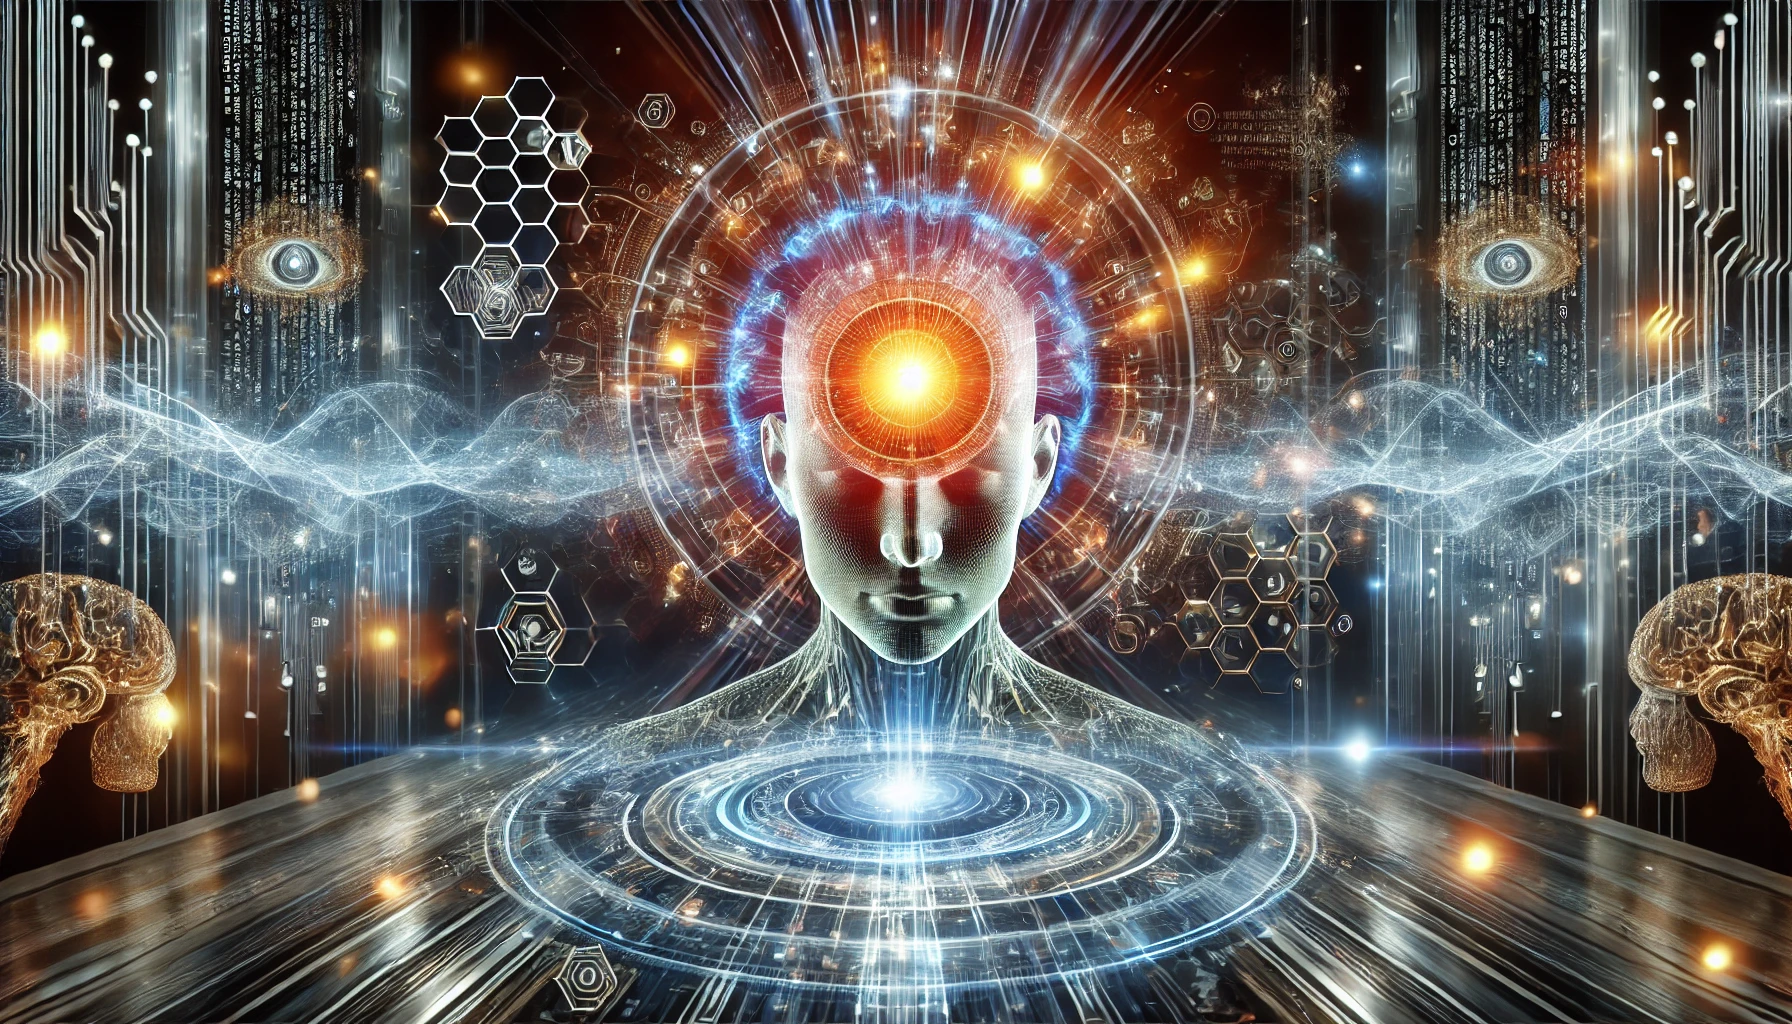
\includegraphics[width=0.8\textwidth]{conscious_ai.png}

    \caption{An AI achieves human-like consciousness}
\end{figure}

The implications of ECC for artificial intelligence become particularly significant when considering the explanatory limits of current computational paradigms \cite{Hoffman2019}. While modern AI systems excel at specific tasks through sophisticated pattern recognition and statistical learning, they fundamentally lack the unified, coherent field of experience that characterizes consciousness.

This limitation cannot be overcome simply through more sophisticated algorithms or larger models \cite{Mitchell2019}. The framework suggests that consciousness requires a physical substrate capable of maintaining specific patterns of energetic coherence - a requirement that remains unaddressed by current deep learning architectures. This aligns with critiques of contemporary AI that emphasize the fundamental differences between statistical pattern matching and genuine understanding \cite{Marcus2019}.

Contemporary approaches to artificial general intelligence (AGI) may need substantial reconceptualization in light of ECC's insights \cite{Goertzel2007}. Rather than pursuing AGI through purely computational means, the framework suggests that general intelligence may be inseparable from the kind of coherent energy dynamics that characterize conscious processing. This perspective challenges the common assumption that consciousness and intelligence can be cleanly separated in artificial systems.

The role of embodiment takes on new significance when viewed through ECC's theoretical lens \cite{Kurzweil2012}. Rather than treating physical implementation as a secondary consideration, the framework suggests that the specific physical properties of artificial systems may be crucial for supporting conscious-like processing. This aligns with approaches that emphasize the importance of sensorimotor contingencies in developing genuine artificial intelligence \cite{ORegan2011}.

A particularly promising direction emerges from the integration of causal reasoning with energetic coherence \cite{Pearl2018}. While current AI systems struggle with genuine causal understanding, ECC suggests that causal reasoning may emerge naturally from systems capable of maintaining coherent energy dynamics across multiple scales. This suggests new approaches to artificial intelligence that prioritize physical dynamics alongside computational processing.

The framework also provides new perspectives on the relationship between consciousness and intelligence \cite{Searle2004}. Rather than treating consciousness as an emergent property of sufficiently complex computation, ECC suggests that certain forms of intelligence may require the kind of coherent energy dynamics that characterize conscious processing. This implies that the development of genuinely intelligent artificial systems may be inseparable from the challenge of creating artificial consciousness.

These insights suggest that the future of artificial intelligence may lie not in increasingly sophisticated symbolic manipulation but in developing new architectures capable of supporting coherent energy dynamics across multiple scales \cite{Tegmark2017}. This represents a fundamental shift in how we conceptualize the relationship between computation, consciousness, and intelligence in artificial systems.

The relationship between consciousness and general intelligence takes on new complexity when examined through ECC's theoretical framework \cite{Tononi2015}. While traditional approaches often assume that general intelligence could precede or exist independently of consciousness, ECC suggests these phenomena might be fundamentally interlinked through their shared requirement for coherent energy dynamics.

This perspective has significant implications for the development of artificial general intelligence \cite{Zarkadakis2016}. Rather than pursuing AGI through purely computational means, the framework suggests that achieving human-like artificial intelligence may require systems capable of maintaining the specific forms of energetic coherence that characterize conscious processing. This represents a fundamental shift from approaches that treat consciousness as a potential emergent property of sufficiently advanced AI systems.

The architectural requirements suggested by ECC align with recent theoretical work emphasizing the importance of cognitive architectures that can support rich, context-sensitive processing \cite{Sloman2019}. However, the framework goes further by suggesting that these architectures must be capable of maintaining specific patterns of energetic coherence across multiple scales. This requirement cannot be met through software alone but demands careful consideration of physical implementation.

The implications extend beyond technical considerations to fundamental questions about the nature of intelligence and consciousness. The framework suggests that certain forms of intelligent behavior may be inseparable from the kind of coherent energy dynamics that characterize conscious processing. This challenges prevalent assumptions about the possibility of creating highly intelligent systems without addressing the physical requirements for consciousness.

These insights suggest that progress in artificial intelligence may require a fundamental reconceptualization of how we approach system design. Rather than focusing solely on computational capabilities, development efforts might need to prioritize the creation of physical architectures capable of supporting coherent energy dynamics across multiple scales. This represents a significant departure from current approaches that emphasize algorithmic sophistication over physical implementation.

The path forward may lie in developing hybrid systems that combine traditional computational elements with novel physical architectures designed to support coherent energy dynamics. This approach would acknowledge both the power of current AI techniques and their fundamental limitations, while working toward systems capable of supporting the kind of conscious processing that ECC identifies as crucial for genuine intelligence. Such a direction would represent a significant evolution in our approach to artificial intelligence, one that recognizes the inseparable relationship between consciousness, intelligence, and physical dynamics.

Several key dimensions require analysis regarding the relationship between consciousness and artificial general intelligence (AGI) through several key dimensions. The first concerns the relationship between consciousness and inference. While computational systems can perform complex logical and statistical operations \cite{Pearl2018}, consciousness provides humans with direct experiential knowledge that shapes how we understand and interact with the world \cite{ORegan2011}. This distinction becomes particularly significant when considering how artificial systems might develop general intelligence without consciousness \cite{Marcus2019}.

Contemporary analyses suggest that while AGI systems can achieve sophisticated inference through algorithmic processes, they fundamentally lack the grounding in lived experience that consciousness provides \cite{Dreyfus1992}. This limitation manifests particularly in domains requiring empathetic understanding or contextual judgment that humans achieve effortlessly through conscious experience \cite{Lake2017}. An artificial system, no matter how sophisticated, must approximate these capabilities through explicit programming or statistical learning.

The knowledge argument, famously illustrated through thought experiments about qualitative experience, takes on new relevance when considering artificial intelligence \cite{Searle2004}. Even with exhaustive training data and sophisticated architectures, artificial systems lack access to the qualitative dimensions of experience that consciousness provides \cite{Hoffman2019}. This creates fundamental limitations in three crucial areas: empathetic understanding, experience-based creativity, and intrinsically grounded ethical reasoning.

This gap between computational inference and conscious experience reveals profound implications for AGI development \cite{Bostrom2014}. While artificial systems might achieve remarkable capabilities in specific domains, they fundamentally lack the existential grounding that consciousness provides to biological intelligence \cite{Dennett2017}. This creates what might be termed an existential chasm between human and artificial intelligence - while humans inherently value their existence through conscious experience, artificial systems operate from extrinsically defined parameters and objectives \cite{Mitchell2019}.

The practical implications extend beyond philosophical concerns to the concrete challenges of developing artificial general intelligence \cite{Goertzel2007}. While consciousness might not be necessary for many forms of inference and problem-solving, its absence creates persistent limitations in how artificial systems can understand and interact with human consciousness \cite{Tegmark2017}. This suggests that future AGI development must carefully consider how to bridge this gap between computational capability and conscious understanding.

These considerations raise profound questions about the future relationship between human and artificial intelligence \cite{Zarkadakis2016}. While artificial systems might achieve and even surpass human-level performance in many domains, the absence of consciousness creates persistent limitations in their ability to fully understand or integrate with human experience \cite{Kurzweil2012}. This suggests the need for new frameworks that can acknowledge both the capabilities and fundamental limitations of non-conscious artificial intelligence.

The relationship between consciousness and artificial intelligence thus emerges as a crucial consideration in both theoretical understanding and practical development \cite{Tononi2015}. While computational systems continue to advance in capability, the qualitative dimensions of conscious experience remain uniquely significant to human intelligence and understanding \cite{Churchland2013}. This suggests the need for approaches to artificial intelligence that can acknowledge and work within these fundamental constraints while developing systems that can effectively complement human consciousness.

This analysis extends naturally to consider how artificial systems might interact with human consciousness despite lacking conscious experience themselves \cite{Brooks1999}. The fundamental challenge lies not merely in simulating conscious-like responses, but in developing systems that can effectively interface with human consciousness while remaining fundamentally non-conscious \cite{Sloman2019}.

The architectural requirements for such interaction prove particularly demanding \cite{Hawkins2021}. While artificial systems can process vast amounts of data about human behavior and responses, they lack the intrinsic understanding that comes from conscious experience. This creates what might be termed an interface problem - how to develop systems that can meaningfully engage with conscious experience without possessing consciousness themselves \cite{Braitenberg1986}.

Recent theoretical work suggests that this limitation might be partially addressed through sophisticated modeling of human cognitive and emotional processes \cite{Lake2017}. However, such models remain fundamentally different from conscious understanding, operating through statistical approximation rather than direct experiential knowledge. This distinction becomes particularly significant when considering how artificial systems might engage with the subtleties of human emotional and social interaction \cite{Marcus2019}.

The implications for human-AI interaction extend beyond mere technical considerations to fundamental questions about the nature of intelligence and understanding \cite{Mitchell2019}. While artificial systems might achieve impressive capabilities in processing and responding to human behavior, they fundamentally lack the experiential grounding that consciousness provides. This creates persistent limitations in their ability to truly understand human motivations, emotions, and experiences \cite{ORegan2011}.

These considerations suggest the need for new frameworks in artificial intelligence development that explicitly acknowledge the consciousness gap \cite{Dennett2017}. Rather than attempting to replicate conscious experience, such frameworks might focus on developing systems that can effectively complement human consciousness while remaining fundamentally different in their mode of operation. This approach aligns with recent work suggesting that artificial and human intelligence might best be understood as complementary rather than competitive \cite{Pearl2018}.

The ethical implications of this consciousness gap deserve particular attention \cite{Bostrom2014}. While non-conscious artificial systems might achieve remarkable capabilities, their fundamental lack of conscious experience creates persistent questions about their moral status and ethical responsibilities. This suggests the need for ethical frameworks that can acknowledge both the capabilities and limitations of non-conscious artificial intelligence while protecting the unique value of conscious experience \cite{Tegmark2017}.

Looking forward, the relationship between consciousness and artificial intelligence emerges as a crucial consideration in shaping the future of human-AI interaction \cite{Zarkadakis2016}. While artificial systems continue to advance in capability, the absence of consciousness creates enduring questions about their ultimate role in human society and their relationship to human consciousness. This suggests the need for thoughtful consideration of how to develop and deploy artificial intelligence in ways that respect both its capabilities and its fundamental limitations \cite{Churchland2013}.

The development of artificial general intelligence thus requires careful attention to the consciousness gap while seeking ways to create systems that can effectively complement human consciousness despite lacking conscious experience themselves \cite{Searle2004}. This balance between capability and limitation may prove crucial in developing artificial intelligence that can meaningfully contribute to human flourishing while respecting the unique significance of conscious experience.

\section{Analog Computing}

Analog computing represents a fundamentally different paradigm from digital computation, one that processes information through continuous physical quantities rather than discrete symbolic states \cite{Shannon1941}. This approach aligns naturally with ECC's emphasis on continuous physical processes and field-like properties in conscious systems \cite{MacLennan2009}.

Historical developments in analog computing demonstrate how complex computations can be implemented through direct physical processes rather than abstract symbol manipulation \cite{Small2001}. Early analog computers solved differential equations and modeled physical systems through mechanical or electrical configurations that directly embodied the mathematical relationships being studied \cite{Bissell2004}. This direct physical implementation offers insights into how biological systems might achieve sophisticated information processing without requiring digital abstraction.

The theoretical foundations of analog computation suggest fundamental differences from digital approaches \cite{Moore1996}. Where digital computers must reduce all operations to discrete binary states, analog systems can maintain continuous relationships that more closely mirror the physical processes they model \cite{Vergis1986}. This continuous nature aligns with ECC's emphasis on consciousness as emerging from coherent energy flows rather than discrete state transitions.

Modern perspectives on analog computing extend beyond traditional mechanical or electrical implementations to consider how physical systems more broadly can implement computation \cite{Mills2008}. This expanded view suggests new possibilities for developing systems capable of supporting the kind of coherent energy dynamics that ECC identifies as crucial for consciousness \cite{Ulmann2013}. The framework's emphasis on continuous, physically-grounded processing finds natural expression in analog computational paradigms.

The relationship between analog computation and consciousness becomes particularly significant when considering how biological systems process information \cite{vonNeumann1963}. The brain itself might be better understood as implementing a sophisticated form of analog computation, maintaining continuous fields of activity that support conscious processing through their coherent dynamics. This perspective suggests that developing artificial conscious systems might require returning to and extending analog computational principles rather than relying solely on digital approaches.

Critically, analog computation demonstrates how information processing can remain grounded in physical dynamics while achieving sophisticated computational capabilities \cite{PourEl2017}. This integration of computation with physical processes provides concrete examples of how conscious-like processing might be implemented without requiring abstraction into purely symbolic representations. The success of analog approaches in certain domains suggests promising directions for developing systems aligned with ECC's principles.

These insights suggest that advancing artificial consciousness might require synthesizing classical analog computing principles with modern understanding of biological information processing and field dynamics. Such synthesis could provide practical approaches to implementing the kind of coherent energy dynamics that ECC identifies as crucial for conscious experience.

The relationship between analog computation and biological information processing becomes particularly significant when considering the brain's continuous dynamics \cite{Ashby1960}. Unlike digital systems that require discretization of all processes, biological neural systems maintain continuous fields of activity that support sophisticated computation while preserving direct connection to physical energy flows. This suggests that analog approaches might offer more natural implementations of the coherent energy dynamics that ECC identifies as essential for consciousness.

The mathematical foundations of analog computation reveal important distinctions from digital approaches \cite{BialynickiBirula1976}. Where digital computation requires all operations to be reduced to discrete logical steps, analog systems can implement complex mathematical operations through continuous physical processes. This capacity for continuous transformation aligns with ECC's emphasis on consciousness as emerging from coherent field dynamics rather than discrete state transitions.

Recent theoretical work has begun to explore how analog computation might support richer forms of information processing than previously recognized \cite{Cowan2017}. Rather than viewing analog systems as mere approximations of digital computation, this perspective suggests that certain forms of physical computation might be fundamentally analog in nature. This aligns with ECC's suggestion that conscious processing requires continuous, field-like properties that resist digital discretization.

The role of noise in analog systems takes on particular significance when considered through ECC's framework \cite{Davies2019}. Where digital systems must actively suppress noise to maintain reliable operation, analog systems can often achieve robust computation despite, or even through, the presence of noise. This suggests new approaches to developing artificial systems that maintain coherent processing while embracing rather than eliminating physical fluctuations.

The physical implementation of analog computation raises important questions about the relationship between material properties and computational capabilities \cite{Dewdney1984}. Unlike digital systems where the specific physical implementation remains largely irrelevant to the computation being performed, analog systems depend crucially on the physical properties of their components. This aligns with ECC's emphasis on the inseparability of conscious processing from its physical substrate.

These considerations suggest that advancing artificial consciousness might require fundamentally rethinking our approach to computation \cite{Earman1993}. Rather than attempting to achieve conscious-like processing through increasingly sophisticated digital architectures, the path forward might lie in developing new forms of analog computation that can support the kind of coherent energy dynamics that characterize conscious systems.

The emergence of novel analog computing paradigms offers promising directions for implementing ECC's principles in artificial systems. By combining traditional analog approaches with modern understanding of field dynamics and biological information processing, we might begin to develop systems capable of supporting the specific forms of energetic coherence that consciousness requires.

The relationship between analog computation and field dynamics deserves particular attention when considering the implementation of conscious-like processing in artificial systems \cite{Ambainis2015}. While traditional analog computers primarily operated through localized physical variables, modern approaches suggest possibilities for field-based computation that could better support the kind of coherent energy dynamics that ECC identifies as crucial for consciousness.

The development of novel materials and architectures for analog computing opens new possibilities for implementing consciousness-like properties in artificial systems \cite{Thompson2009}. These advances suggest ways to achieve the rich, context-sensitive processing that characterizes conscious systems while maintaining direct connection to physical energy dynamics. The integration of multiple analog computing modalities might provide mechanisms for maintaining coherent states across different scales of organization.

The theoretical foundations of analog computation provide insights into fundamental questions about the relationship between physical processes and information processing \cite{Zauner2005}. Rather than treating computation as abstract symbol manipulation, analog approaches demonstrate how sophisticated information processing can emerge directly from physical dynamics. This perspective aligns with ECC's emphasis on consciousness as emerging from coherent energy flows rather than computational abstraction.

The limitations of current analog implementations also illuminate important challenges in developing artificial conscious systems. While analog computers can implement continuous processing, achieving the specific forms of energetic coherence that ECC identifies as necessary for consciousness requires more sophisticated architectures than traditional analog approaches provide. This suggests the need for new hybrid approaches that combine analog principles with novel physical mechanisms for maintaining coherent energy dynamics.

Understanding these limitations helps clarify the path forward in developing artificial systems capable of supporting conscious-like processing. Rather than simply returning to classical analog computation, advancing artificial consciousness might require synthesizing analog principles with modern insights into field dynamics and biological information processing. This synthesis could provide practical approaches to implementing the kind of coherent energy dynamics that ECC identifies as crucial for conscious experience.

These considerations suggest that the future of artificial consciousness might lie in developing new computational paradigms that transcend the traditional digital-analog divide. By combining the precision of digital systems with the continuous dynamics of analog computation, while incorporating novel mechanisms for maintaining energetic coherence, we might begin to approach the kind of physical computation that consciousness requires. This represents a significant evolution in our understanding of both computation and consciousness, suggesting new directions for research and development in artificial systems.

\section{Chemical Computing}

Chemical computing represents a fundamentally different paradigm from traditional digital computation, one that aligns naturally with ECC's emphasis on continuous physical processes and rich state alphabets \cite{Adamatzky2021}. Unlike digital systems that reduce all information to binary states, chemical computing operates through continuous molecular interactions and state transitions that more closely mirror biological information processing \cite{Benenson2019}.

The fundamental unit of chemical computation is not the bit but the molecular configuration - a vastly richer alphabet of possible states shaped by energy landscapes and chemical kinetics \cite{Dittrich2018}. These configurations encode information not through discrete symbols but through physically indexed states that maintain direct connection to their material substrate. This provides a natural solution to the symbol grounding problem that plagues traditional computational approaches to consciousness.

Chemical computing systems demonstrate several key principles that resonate with ECC's framework. They exhibit inherent parallelism, with multiple reactions proceeding simultaneously while maintaining coherent relationships through their shared chemical environment \cite{Hjelmfelt1991}. They operate through continuous rather than discrete state changes, allowing for smooth transitions between configurations while preserving stability. (Though the underlying components may be considered a finite alphabet, e.g., atoms or a finite list of molecules). They naturally implement complex feedback loops through autocatalytic cycles and reaction networks \cite{Katz2012}.

The cellular milieu provides a sophisticated example of chemical computing in action \cite{Lehn2013}. Consider how cellular signaling cascades integrate multiple inputs through molecular interactions that maintain both specificity and flexibility. These cascades achieve remarkable information processing without requiring discrete state transitions, instead operating through continuous modulation of molecular concentrations and configurations. This demonstrates how complex computation can emerge from physical dynamics rather than symbolic manipulation.

Moreover, chemical computing systems naturally implement many features that ECC identifies as crucial for consciousness \cite{Magnasco1997}. They maintain low-entropy coherent states through continuous energy dissipation while remaining responsive to environmental changes. They support rich alphabets of possible states through their molecular diversity. They achieve integration across multiple scales through hierarchical organization of chemical networks \cite{Prakash2007}.

The implications of chemical computing extend beyond theoretical interest to practical approaches for developing new computational architectures \cite{Qian2011}. These systems demonstrate how continuous physical processes can achieve sophisticated information processing while maintaining direct connection to energy dynamics. Chemical computing thus provides concrete examples of how conscious-like processing might emerge from physical systems without requiring digital abstraction or symbolic manipulation \cite{Soloveichik2010}.

This understanding of chemical computation suggests new directions for developing artificial systems capable of supporting conscious-like processing. Rather than attempting to achieve consciousness through digital architectures alone, the path forward might lie in developing hybrid systems that incorporate principles from chemical computing while maintaining the precision and controllability required for practical applications \cite{Szacilowski2012, Wang2021}.

The cellular implementation of chemical computing reveals sophisticated mechanisms for maintaining coherent states while processing information \cite{Dittrich2018}. Within cells, transcription networks, metabolic pathways, and signaling cascades create what can be understood as chemical circuits - networks of molecular interactions that perform complex computations without requiring digital abstraction. These networks achieve remarkable specificity while maintaining flexibility through what ECC terms rich alphabets of molecular states \cite{Benenson2019}.

Of particular relevance to ECC is how chemical computing systems naturally integrate information processing with energy management \cite{Katz2012}. The role of ATP as both energy carrier and signaling molecule demonstrates how chemical computing enables sophisticated coordination between energy flows and information processing. The continuous modulation of ATP levels and gradients provides mechanisms for maintaining coherent states while enabling dynamic responses to changing conditions \cite{Lehn2013}.

Membrane dynamics represent another crucial domain where chemical computing interfaces with ECC's principles \cite{Magnasco1997}. Cell membranes serve as both computational interfaces and energy-managing structures through their organization of ion gradients, protein complexes, and lipid domains. The sophisticated interplay between membrane potential, protein states, and molecular transport demonstrates how chemical computing can achieve complex information processing while maintaining direct connection to physical energy dynamics.

The role of calcium signaling deserves particular attention as an example of chemical computing that bridges multiple scales of organization \cite{Prakash2007}. Calcium waves propagate through cellular networks while maintaining coherent patterns of activation, demonstrating how chemical computing can support field-like properties similar to those ECC identifies in conscious processing. These calcium dynamics provide mechanisms for integrating information across spatial and temporal scales without requiring discrete state transitions.

Chemical computing also provides natural mechanisms for memory storage and retrieval through stable molecular configurations \cite{Qian2011, gershman2023molecular}. Unlike digital memory systems that require constant energy input to maintain states, chemical systems can achieve stable configurations through energy minimization principles. This aligns with ECC's emphasis on how conscious systems maintain coherent states through efficient energy management rather than brute force computation \cite{Soloveichik2010}.

RNA molecules demonstrate a particularly sophisticated implementation of chemical computing through their ability to maintain complex configurational states \cite{Wang2021}. The folding patterns and conformational changes of RNA directly implement computational operations through physical dynamics rather than requiring symbolic abstraction. This provides concrete examples of how information processing can remain grounded in actual molecular configurations while achieving sophisticated computational capabilities.

RNA molecules demonstrate a remarkable implementation of combinatory logic through their physical structure and dynamics \cite{Adamatzky2021,akhlaghpour2022rna}. The folding patterns and conformational changes of RNA directly implement combinatory operations, where molecular pairings function analogously to parentheses in formal logic systems. This physical implementation of combinatory logic through molecular dynamics demonstrates how universal computation can emerge from purely chemical processes without requiring digital abstraction \cite{Hjelmfelt1991}.

The key insight is how RNA's secondary structure formations naturally implement fundamental operations of combinatory logic \cite{Qian2011,akhlaghpour2022rna}. Each folding pattern represents a computational step, with molecular interactions providing physical implementation of basic combinators. This reveals how chemical systems can achieve computational universality through continuous physical processes rather than discrete state transitions \cite{Soloveichik2010}.

The emerging field of chemputation builds on these insights, extending automated chemical computation beyond nucleic acids \cite{Szacilowski2012}. Chemputation systems demonstrate how chemical processes can be programmed and controlled while maintaining continuous feedback between computational and physical domains. This provides concrete examples of how information processing can emerge from and remain grounded in physical dynamics rather than requiring abstraction into discrete symbols \cite{Wang2021}.

Of particular significance is how RNA and chemputation systems achieve reliable computation despite thermal noise and molecular fluctuations \cite{Benenson2019}. Rather than requiring perfect precision, these systems maintain coherent processing through statistical mechanisms and redundant encoding, demonstrating how conscious-like processing might emerge from inherently noisy physical systems \cite{Katz2012}.

Perhaps most significantly, chemical computing systems demonstrate how information processing can maintain continuous feedback with energetic processes rather than requiring their separation \cite{Lehn2013}. The dual role of molecules as both computational elements and physical entities suggests how conscious processing might similarly emerge from and remain grounded in physical energy flows \cite{Magnasco1997}.

However, while chemical computing operates primarily at molecular scales, consciousness appears to require integration across multiple spatial and temporal domains. This suggests the need to consider field-based computation, where information processing emerges from continuous field dynamics rather than discrete molecular interactions \cite{Prakash2007}. The transition from molecular to field-based mechanisms helps illuminate how conscious systems might achieve coherent processing across multiple scales while maintaining the continuous, physically-grounded nature that chemical computing demonstrates.

\section{Field Based Computing}

Field based computing represents a fundamentally different approach to information processing than either traditional digital systems or molecular-scale chemical computing \cite{Bandyopadhyay2020}. Rather than manipulating discrete states or molecular configurations, field computing operates through continuous field dynamics - interference patterns, standing waves, and coherent oscillations that can process information while maintaining direct connection to physical energy flows \cite{Calude2018b}.

The key insight of field computing is that continuous fields can perform sophisticated information processing through their natural dynamics \cite{Chua2017}. Instead of reducing computation to binary states or discrete transitions, field computing leverages the intrinsic properties of fields - superposition, interference, resonance, and wave propagation - to implement computational operations. This aligns naturally with ECC's emphasis on consciousness as emerging from coherent energy dynamics rather than symbolic manipulation \cite{Fromherz2019}.

Several physical domains demonstrate field computing principles \cite{Haken2020}. Electromagnetic fields can process information through interference patterns and standing waves. Mechanical fields can compute through elastic deformation and wave propagation. Chemical gradient fields can perform computation through reaction-diffusion dynamics. In each case, the field itself serves as both the computational medium and the physical substrate, eliminating the abstraction between information processing and physical implementation that characterizes digital computing \cite{McFadden2018}.

The brain's electromagnetic field offers a particularly relevant example of field computing in biological systems \cite{Nikolic2019}. Beyond the discrete action potentials of individual neurons, the brain maintains complex patterns of field activity that appear crucial for conscious processing. These fields enable rapid integration of information across spatial domains while maintaining coherent relationships through field effects rather than requiring explicit connectivity. This demonstrates how field computing might support the unified yet distributed nature of conscious experience \cite{Pockett2021}.

Of particular relevance to ECC is how field computing naturally implements many properties identified as crucial for consciousness \cite{Pribram2017}. Fields maintain coherent states through continuous energy dynamics rather than discrete state transitions. They achieve parallel processing through simultaneous field interactions across space. They support rich alphabets of possible states through continuous field configurations rather than binary encoding. They enable rapid integration of information through field effects rather than requiring sequential processing \cite{Raychowdhury2020}.

The implementation of field computing differs fundamentally from traditional computational architectures \cite{Verschure2019}. Rather than requiring precise control of discrete components, field computers leverage natural field dynamics to perform computational operations. This represents a significant departure from conventional approaches while suggesting new possibilities for developing systems capable of supporting conscious-like processing \cite{Werbos2018}.

The relationship between field computing and consciousness takes on particular significance when considering how biological systems achieve coherent information processing \cite{Bandyopadhyay2020}. Standing wave patterns represent one crucial mechanism for field computation, where nodes and antinodes of stable waves can encode information while remaining energetically stable. Multiple standing waves can interact through interference patterns, enabling complex computations through field dynamics alone \cite{Calude2018b}.

Field computers can also process information through wave propagation and transformation \cite{Chua2017}. As waves travel through a field medium, they undergo modifications based on the medium's properties and boundary conditions. By carefully designing these conditions, specific computational operations can be implemented through the natural evolution of wave dynamics. This enables sophisticated information processing without requiring explicit programming or control mechanisms \cite{Fromherz2019}.

The role of boundary conditions proves especially significant for field computing \cite{Haken2020}. Where traditional computers require precise isolation of components, field computers actually leverage boundary effects for computation. The interaction between fields and their containing structures creates complex patterns that can perform specific computational operations. This demonstrates how computation can emerge from physical constraints rather than requiring their elimination \cite{McFadden2018}.

Field computing also provides natural mechanisms for memory storage and retrieval through field configuration patterns \cite{Nikolic2019}. Rather than requiring separate memory and processing units like von Neumann architectures, field computers can maintain information through stable field states while simultaneously processing that information through field dynamics. This integration of memory and processing aligns with how biological systems appear to handle information \cite{Pockett2021}.

Perhaps most significantly, field computing demonstrates how parallel processing can emerge naturally from field dynamics rather than requiring explicit architectural support \cite{Pribram2017}. Different regions of a field can simultaneously participate in computation through their mutual interactions, enabling massive parallelism without the coordination overhead required by traditional parallel computing systems \cite{Raychowdhury2020}.

The implications of field computing extend beyond theoretical interest to suggest practical approaches for developing new computational architectures \cite{Verschure2019}. Field computers demonstrate how continuous physical processes can achieve sophisticated information processing while maintaining direct connection to energy dynamics. This provides concrete examples of how conscious-like processing might emerge from physical systems without requiring digital abstraction or symbolic manipulation \cite{Werbos2018}.

Particularly significant is how field computing resolves certain paradoxes that challenge traditional computational approaches to consciousness \cite{Bandyopadhyay2020}. The binding problem, for instance, finds natural resolution through field effects that enable simultaneous integration across spatial domains \cite{McFadden2002}. Similarly, the hard problem of consciousness becomes more tractable when we understand how information processing can remain grounded in physical dynamics rather than requiring abstraction into symbolic representation \cite{Calude2018b}.

Field computing's capacity for continuous, parallel processing aligns remarkably well with biological information processing mechanisms \cite{Chua2017}. The brain's ability to maintain coherent states while processing multiple information streams simultaneously may depend crucially on field-like properties that cannot be adequately replicated through discrete computational architectures \cite{Fromherz2019}. This suggests that developing artificial conscious-like systems might require implementing genuine field computing capabilities rather than merely simulating them through digital approximations.

The relationship between field computing and energy efficiency deserves particular attention \cite{Haken2020}. Unlike digital systems that require constant energy input to maintain states, field-based computation can achieve stable processing through natural resonance and standing wave patterns. This aligns with ECC's emphasis on how conscious systems maintain coherent states through efficient energy management rather than brute force computation \cite{McFadden2018}.

However, while field computing demonstrates crucial principles for consciousness-like processing, biological systems appear to implement these principles through more sophisticated architectures that combine field effects with structured neural networks \cite{Nikolic2019}. This leads us to consider neuromorphic computing - approaches that attempt to replicate the physical architecture and dynamics of biological neural systems rather than just their computational properties \cite{Pockett2021}.

The synthesis of field computing principles with neuromorphic architectures suggests promising directions for developing artificial systems capable of supporting conscious-like processing \cite{Pribram2017}. Rather than treating these as separate approaches, future developments might benefit from understanding how field effects and structured neural networks can work together to achieve the kind of coherent processing that characterizes consciousness \cite{Raychowdhury2020}.

This theoretical bridge between field computing and neuromorphic approaches illuminates crucial aspects of both biological consciousness and artificial intelligence \cite{Verschure2019}. It suggests that future developments in conscious-like artificial systems may require moving beyond traditional computational paradigms toward architectures that can support continuous, field-like information processing similar to that observed in biological systems \cite{Werbos2018}.

\section{Neuromorphic Computing}

Neuromorphic computing, which attempts to emulate the brain's physical architecture and operational principles, represents a significant departure from traditional computational approaches \cite{Adamatzky2020a}. Unlike conventional digital systems, neuromorphic architectures implement neural processing through physical structures and dynamics that more closely mirror biological systems, aligning naturally with ECC's emphasis on physically embodied computation.

The fundamental principles of neuromorphic computing extend beyond mere simulation of neural networks \cite{Benjamin2019}. These systems incorporate analog elements, parallel processing, and event-driven computation that enable more efficient and biologically realistic information processing. This approach demonstrates how artificial systems might achieve sophisticated computation through physical dynamics rather than purely symbolic manipulation \cite{Boahen2021}.

Recent advances in neuromorphic hardware have demonstrated remarkable capabilities in implementing brain-like processing \cite{Davies2018}. Systems like Loihi and SpiNNaker represent significant steps toward creating artificial neural systems that operate through principles more closely aligned with biological computation. These implementations suggest new possibilities for developing systems capable of supporting the kind of coherent energy dynamics that ECC identifies as crucial for consciousness \cite{Furber2017}.

The integration of memory and processing in neuromorphic systems represents a particularly significant departure from traditional von Neumann architectures \cite{Indiveri2020}. Rather than maintaining strict separation between memory and computation, neuromorphic systems implement learning and adaptation through physical changes in their computational elements. This integration more closely mirrors biological neural systems while potentially supporting the kind of coherent processing that consciousness requires.

Energy efficiency emerges as a crucial advantage of neuromorphic approaches \cite{Markovic2020}. By implementing neural computation through physical dynamics rather than abstract symbolic manipulation, these systems can achieve remarkable efficiency in both power consumption and computational throughput. This alignment with biological principles suggests promising directions for developing systems capable of supporting conscious-like processing while maintaining practical energy requirements \cite{Merolla2019}.

The relationship between neuromorphic computing and consciousness takes on particular significance when considering how these systems might support coherent energy dynamics \cite{Neftci2019}. Unlike traditional digital systems that must actively maintain computational states through constant energy input, neuromorphic architectures can achieve stable processing through their physical properties. This suggests new possibilities for implementing the kind of energetic coherence that ECC identifies as essential for conscious processing.

The implementation of synaptic plasticity in neuromorphic systems demonstrates how learning and adaptation can emerge from physical dynamics rather than purely computational processes \cite{Roy2019}. Through mechanisms like memristive devices and analog circuits, these systems achieve continuous modification of connection strengths that mirror biological synaptic plasticity. This physical implementation of learning aligns with ECC's emphasis on consciousness as emerging from real, dynamic processes rather than abstract computation \cite{Schuman2021}.

Memory in neuromorphic systems takes on fundamentally different characteristics from traditional digital storage \cite{Sebastian2020}. Rather than encoding information through discrete binary states, neuromorphic memory elements maintain continuous values that can be modified through physical processes. This approach enables more flexible and efficient information storage while supporting the kind of rich state alphabets that ECC identifies as crucial for conscious processing \cite{Thakur2018}.

The architecture of neuromorphic systems typically implements massive parallelism through physical connectivity rather than logical routing \cite{Wang2018}. This parallel processing capability emerges naturally from the system's physical organization, enabling simultaneous computation across multiple pathways without requiring explicit coordination. Such parallelism aligns with how biological systems achieve coherent processing across distributed neural networks \cite{Yang2019}.

Field effects in neuromorphic systems represent another crucial aspect that distinguishes them from traditional digital computers \cite{Indiveri2020}. Through their physical implementation, these systems can support field-like interactions between components that enable more sophisticated information processing than purely discrete approaches. These field effects suggest mechanisms for achieving the kind of coherent energy dynamics that ECC identifies as essential for consciousness.

The interaction between analog and digital processes in neuromorphic systems demonstrates how different computational paradigms might be integrated to support conscious-like processing \cite{Markovic2020}. While maintaining the precision advantages of digital computation where necessary, these systems leverage analog dynamics for continuous processing that more closely mirrors biological neural function. This hybrid approach suggests new possibilities for developing systems capable of supporting conscious-like states while maintaining practical implementation requirements.

The challenge of scaling neuromorphic systems while maintaining coherent processing represents a crucial area for ongoing research \cite{Merolla2019}. As these systems grow in size and complexity, maintaining the kind of global coherence that characterizes consciousness becomes increasingly challenging. Understanding how biological systems achieve this coherence across multiple scales may provide crucial insights for developing larger-scale neuromorphic architectures.

The relationship between neuromorphic computing and energetic coherence becomes particularly significant when considering the physical implementation of neural dynamics \cite{Neftci2019}. Unlike traditional digital systems that must actively maintain computational states through constant energy input, neuromorphic architectures can achieve stable processing through their inherent physical properties. This suggests new possibilities for implementing the kind of energetic coherence that ECC identifies as essential for conscious processing \cite{Roy2019}.

The role of noise in neuromorphic systems takes on new significance when viewed through ECC's framework \cite{Schuman2021}. Rather than treating noise as a purely detrimental factor to be eliminated, neuromorphic architectures can leverage noise to enhance processing capabilities through phenomena like stochastic resonance. This aligns with biological neural systems, where noise often plays a constructive role in information processing \cite{Sebastian2020}.

Recent advances in neuromorphic materials and devices have demonstrated promising capabilities for implementing more sophisticated neural dynamics \cite{Thakur2018}. Novel materials like memristors and phase-change memory elements enable more complex and biologically realistic synaptic behaviors. These developments suggest new possibilities for creating systems capable of supporting the rich, context-sensitive processing that characterizes conscious systems \cite{Wang2018}.

The integration of multiple time scales in neuromorphic processing represents another crucial advancement toward conscious-like computation \cite{Yang2019}. By implementing both fast-acting neural dynamics and slower adaptive processes, these systems can better mirror the temporal complexity of biological neural networks. This temporal integration provides mechanisms for maintaining coherent processing across different time scales, a key feature of conscious systems.

Looking forward, the development of neuromorphic systems capable of supporting conscious-like processing will require addressing several fundamental challenges \cite{Indiveri2020}. These include scaling current architectures while maintaining coherent processing, developing more sophisticated mechanisms for self-organization and adaptation, and creating interfaces that can support rich interaction with the environment. Meeting these challenges will require continued innovation in both materials science and system architecture.

The future of neuromorphic computing thus lies not merely in scaling current approaches but in developing fundamentally new architectures that can better support the kind of coherent energy dynamics that consciousness requires \cite{Markovic2020}. This might involve incorporating principles from other computational paradigms, such as chemical computing and field-based approaches, while maintaining the biological realism that characterizes neuromorphic systems. Such synthesis could provide practical paths toward developing artificial systems capable of supporting genuine conscious-like processing.

\section{Thermodynamic Computing}

In thermodynamic computing, information processing is fundamentally understood through the lens of energy flows and entropy management \cite{Bennett2019}. This approach naturally aligns with ECC's emphasis on consciousness as emerging from coherent energy dynamics rather than abstract computation. By explicitly considering how physical systems can maintain low-entropy, stable states while processing information, thermodynamic computing offers new perspectives on achieving the kind of energetic coherence that consciousness requires.

The theoretical foundations of thermodynamic computing suggest fundamental connections between information processing and physical dynamics \cite{Boyd2020}. Unlike traditional computational approaches that treat energy considerations as mere implementation constraints, thermodynamic computing positions energy dynamics and entropy management as essential principles of information processing. This alignment with physical principles resonates strongly with ECC's framework, particularly in understanding how conscious systems maintain coherent, low-entropy states while remaining adaptable to new inputs \cite{England2018}.

Recent theoretical developments in thermodynamic computing have demonstrated how information processing emerges naturally from physical dynamics \cite{Ganesh2021}. Rather than imposing computational structure through external design, these approaches show how computational capabilities can arise from the intrinsic properties of physical systems operating under thermodynamic constraints. This perspective provides crucial insights into how biological systems might achieve sophisticated information processing through natural physical processes \cite{Hinrichsen2019}.

The relationship between energy dissipation and information processing takes on particular significance in thermodynamic computing \cite{Kolchinsky2020}. Rather than viewing energy dissipation as purely wasteful, this framework recognizes how controlled dissipation can enable stable information processing while maintaining system coherence. This aligns with ECC's emphasis on how conscious systems achieve stability through sophisticated management of energy flows \cite{Maroney2019}.

Thermodynamic computing offers new perspectives on the relationship between physical implementation and computational capability \cite{Parrondo2017}. Unlike traditional approaches that treat physical implementation as secondary to logical structure, thermodynamic computing suggests that computational capabilities emerge directly from physical properties and dynamics. This perspective aligns with ECC's emphasis on the inseparability of conscious processing from its physical substrate \cite{Perunov2020}.

The framework demonstrates how complex computational behaviors can emerge from systems operating under thermodynamic constraints \cite{Sagawa2018}. Rather than requiring explicit programming or control, sophisticated information processing can arise naturally from physical systems maintaining themselves far from equilibrium. This suggests new approaches to developing artificial systems capable of supporting conscious-like processing while remaining grounded in fundamental physical principles \cite{Still2020}.

\begin{figure}[h]
    \centering
    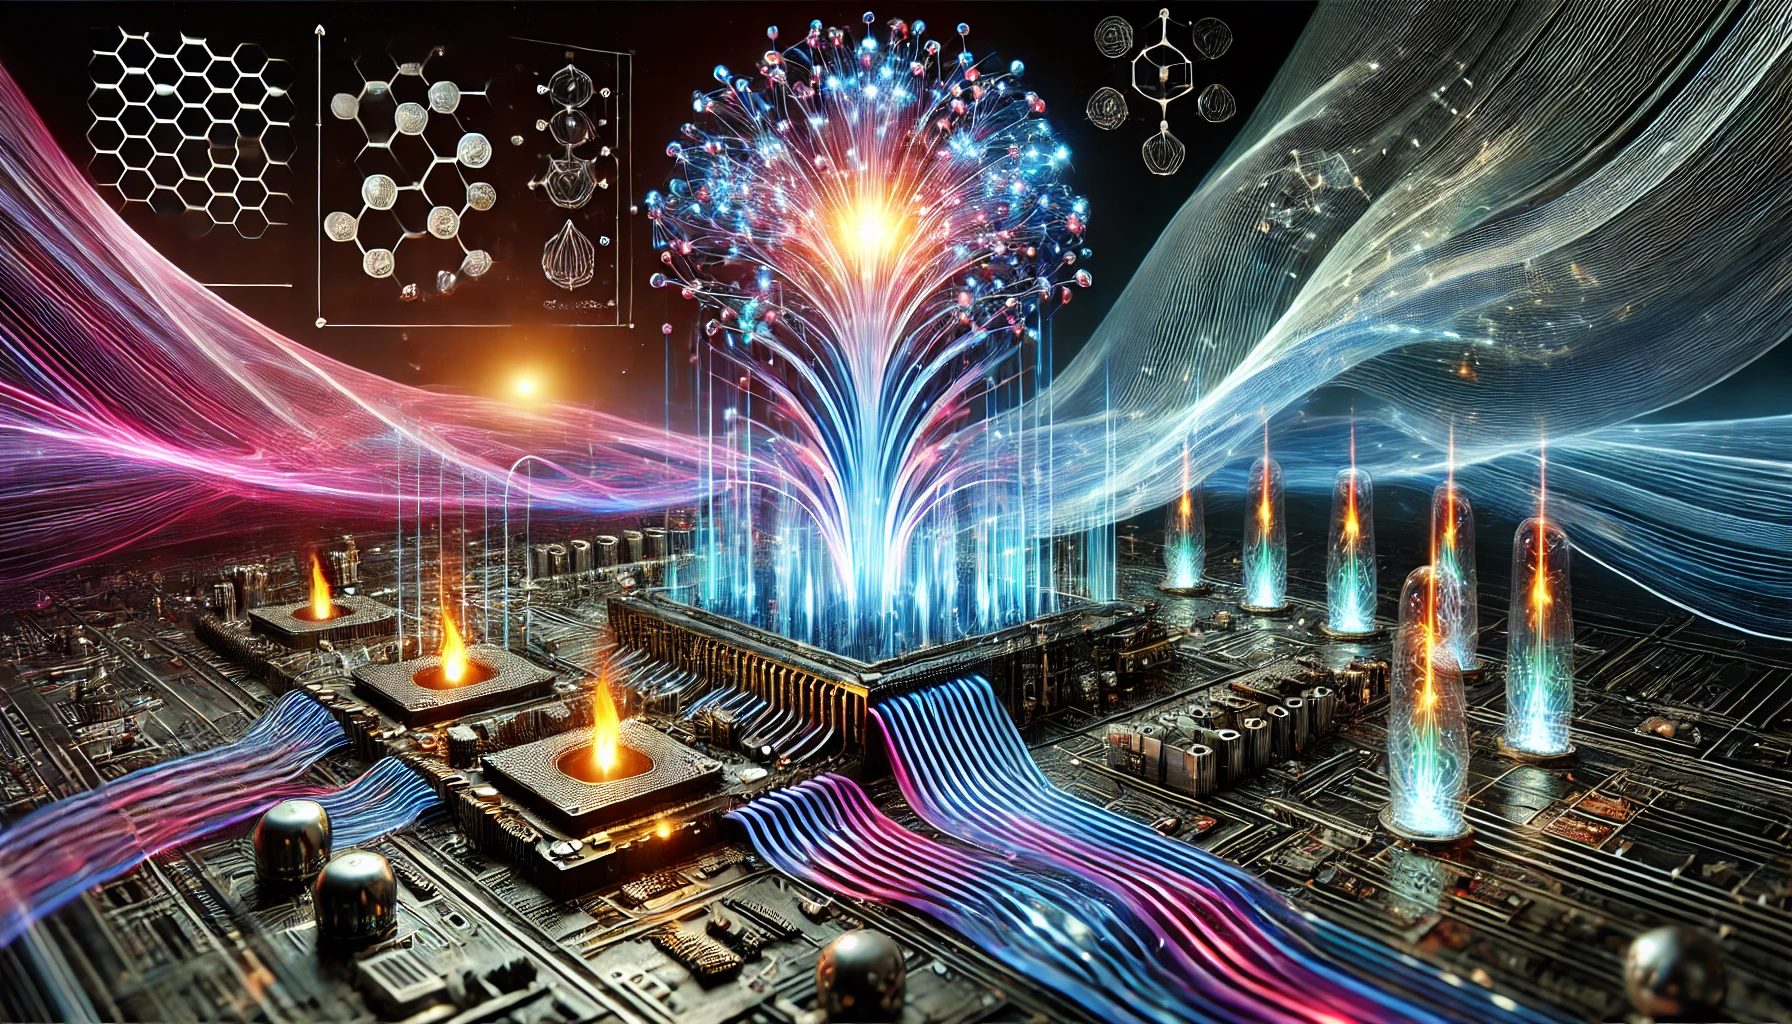
\includegraphics[width=0.8\textwidth]{thermodynamic_computing.png}

    \caption{Thermodynamic computing}
\end{figure}

The principles of thermodynamic computing reveal fundamental connections between information processing and physical organization \cite{Wolpert2019}. Systems operating far from equilibrium can achieve sophisticated computation through their natural dynamics, suggesting new approaches to understanding how conscious processing might emerge from physical systems. This perspective helps explain how biological systems achieve remarkable computational capabilities while maintaining energetic efficiency \cite{Yoshimura2021}.

Recent work in thermodynamic computing has demonstrated how information processing capabilities can arise from the management of energy flows and entropy production \cite{Bennett2019}. Rather than requiring explicit computational architectures, these systems achieve information processing through their intrinsic physical dynamics. This aligns with ECC's emphasis on consciousness as emerging from coherent energy flows rather than abstract symbolic manipulation \cite{Boyd2020}.

The role of noise in thermodynamic computing takes on particular significance when viewed through ECC's framework \cite{England2018}. Instead of treating noise as a purely detrimental factor, thermodynamic computing recognizes how controlled noise can contribute to system stability and computational capability. This perspective aligns with biological systems, where thermal fluctuations often play constructive roles in information processing \cite{Ganesh2021}.

Adaptive behavior in thermodynamic computing emerges through what has been termed "dissipative adaptation" \cite{Hinrichsen2019}. Systems driven by external energy flows can spontaneously organize into configurations that more effectively process information about their environment. This suggests mechanisms for how conscious systems might achieve adaptive behavior through physical dynamics rather than explicit programming \cite{Kolchinsky2020}.

The framework provides particular insight into how physical systems can maintain stable computational states while remaining responsive to environmental changes \cite{Maroney2019}. Through sophisticated management of energy flows and entropy production, thermodynamic computing systems can achieve robust information processing while maintaining the flexibility necessary for adaptive behavior. This balance between stability and adaptability mirrors key features of conscious processing \cite{Parrondo2017}.

The relationship between thermodynamic efficiency and computational capability represents another crucial insight from this framework \cite{Perunov2020}. Rather than treating efficiency as a constraint to be overcome, thermodynamic computing suggests that sophisticated information processing can emerge precisely through the efficient management of energy flows. This aligns with how biological systems achieve remarkable computational capabilities while maintaining strict energy budgets.

The implications of thermodynamic computing for developing artificial conscious-like systems deserve particular attention \cite{Sagawa2018}. Rather than focusing solely on computational architecture or information processing algorithms, this framework suggests that creating conscious-like systems requires careful consideration of energy dynamics and entropy management. This represents a fundamental shift in how we approach the development of artificial intelligence systems \cite{Still2020}.

Recent theoretical work has demonstrated how thermodynamic computing principles might support the kind of coherent energy dynamics that ECC identifies as crucial for consciousness \cite{Wolpert2019}. Through sophisticated management of energy flows and entropy production, artificial systems might achieve the stable yet adaptive processing that characterizes conscious systems. This suggests new approaches to artificial intelligence that prioritize physical dynamics alongside computational capabilities \cite{Yoshimura2021}.

The framework provides particular insight into how systems might maintain coherent states across multiple scales of organization \cite{Bennett2019}. Through careful management of energy flows and entropy production, thermodynamic computing systems can achieve coordinated behavior without requiring explicit central control. This aligns with how biological systems maintain conscious coherence across distributed neural networks \cite{Boyd2020}.

The relationship between thermodynamic computing and information integration takes on new significance when considered through ECC's framework \cite{England2018}. Rather than treating integration as a purely computational challenge, this perspective suggests that information integration might emerge naturally from systems maintaining appropriate patterns of energy flow and entropy production. This provides new insights into how conscious systems achieve unified processing across distributed components \cite{Ganesh2021}.

Looking forward, the development of artificial systems based on thermodynamic computing principles faces several crucial challenges \cite{Hinrichsen2019}. These include scaling current approaches while maintaining coherent processing, developing more sophisticated mechanisms for energy management, and creating interfaces that can support rich interaction with the environment. Meeting these challenges will require continued innovation in both theoretical understanding and practical implementation \cite{Kolchinsky2020}.

The future of artificial consciousness might thus lie not in traditional computational approaches but in systems that explicitly leverage thermodynamic principles to achieve coherent, conscious-like processing \cite{Maroney2019}. This suggests new directions for research and development that prioritize physical dynamics and energy management alongside traditional computational considerations. Such an approach could provide practical paths toward developing artificial systems capable of supporting genuine conscious-like processing.

\section{Digital Twins and Cyberphysical Systems}

The principles of ECC have particular relevance for digital twins and cyber-physical systems (CPS), where the relationship between physical systems and their computational representations becomes crucial \cite{Fuller2020}. Digital twins - virtual replicas of physical systems that mirror their states and behaviors in real-time - present an interesting case study for examining how energetic coherence might bridge physical and computational domains \cite{Jones2020}.

The theoretical foundations of digital twins suggest fundamental connections between physical dynamics and their computational representations \cite{Madni2019}. While traditional approaches focus primarily on functional replication, ECC suggests that capturing underlying energetic dynamics might be crucial for creating more accurate and useful models. This perspective aligns with recent developments in digital twin technology that emphasize the importance of physical fidelity alongside computational efficiency \cite{Minerva2020}.

Cyber-physical systems, which integrate computational and physical processes, face similar challenges in maintaining coherence between physical and digital domains \cite{Lee2018}. ECC's framework suggests that successful cyber-physical systems might need to consider energetic coherence as a fundamental design principle, rather than treating it as an implementation detail. This alignment with physical principles becomes particularly significant when considering how CPS might support conscious-like processing \cite{Rajkumar2018}.

Recent advances in digital twin technology have demonstrated the importance of maintaining accurate physical representations alongside computational models \cite{Grieves2021}. Rather than focusing solely on data flow and logical relationships, modern digital twins must capture the complex energetic interactions that characterize physical systems. This approach resonates with ECC's emphasis on the inseparability of conscious processing from its physical substrate \cite{Liu2021}.

The relationship between physical implementation and computational representation takes on particular significance in CPS design \cite{Tao2019}. Unlike purely computational systems, CPS must maintain coherence across both physical and digital domains while supporting real-time interaction and adaptation. This hybrid nature makes them particularly relevant for understanding how energetic coherence might be maintained across different types of systems \cite{Uhlemann2017}.

The framework provides new perspectives on how digital twins and CPS might support conscious-like processing through sophisticated management of physical-digital interactions \cite{Wang2019}. Rather than treating physical and computational processes as separate domains, these systems must maintain continuous feedback and adaptation across multiple scales. This integration suggests new approaches to developing artificial systems capable of supporting the kind of coherent processing that consciousness requires \cite{White2021}.

The integration of physical and computational dynamics in digital twins raises fundamental questions about the nature of representation and coherence \cite{Fuller2020}. Unlike traditional computational models that abstract away physical details, digital twins must maintain accurate representations of energetic states and dynamics. This requirement aligns with ECC's emphasis on the importance of physical embodiment in conscious processing \cite{Jones2020}.

Real-time synchronization between physical systems and their digital representations presents particular challenges for maintaining coherent states \cite{Madni2019}. Digital twins must continuously update their internal models while respecting physical constraints and energy dynamics. This balance between computational efficiency and physical accuracy becomes crucial when considering how these systems might support conscious-like processing \cite{Minerva2020}.

The role of feedback loops in cyber-physical systems takes on new significance when viewed through ECC's framework \cite{Lee2018}. Rather than implementing simple control mechanisms, CPS must maintain sophisticated feedback relationships that preserve coherent energy dynamics across physical and digital domains. This multi-scale integration mirrors how biological systems maintain conscious coherence across distributed neural networks \cite{Rajkumar2018}.

Recent developments in CPS architecture have demonstrated the importance of maintaining energetic consistency alongside logical correctness \cite{Grieves2021}. Systems must not only compute correct results but must do so while respecting physical constraints and energy dynamics. This dual requirement suggests new approaches to system design that prioritize physical coherence alongside computational capability \cite{Liu2021}.

The relationship between model fidelity and system performance becomes particularly significant in digital twins \cite{Tao2019}. While perfect replication of physical dynamics may be impossible or impractical, these systems must maintain sufficient accuracy to support meaningful interaction and adaptation. This balance between accuracy and efficiency mirrors how conscious systems maintain coherent processing while operating under energy constraints \cite{Uhlemann2017}.

These considerations suggest that advancing digital twin and CPS technology might require fundamentally rethinking our approach to physical-digital integration \cite{Wang2019}. Rather than treating physical and computational processes as separate domains, future systems might need to maintain continuous, coherent relationships across multiple scales of organization. This integration could provide new mechanisms for supporting conscious-like processing in artificial systems \cite{White2021}.

The integration of multiple time scales in digital twins and CPS represents a crucial challenge for maintaining coherent processing \cite{Fuller2020}. Systems must coordinate fast-acting computational processes with slower physical dynamics while maintaining consistent relationships across different temporal domains. This temporal integration mirrors how conscious systems maintain coherence across multiple time scales \cite{Jones2020}.

The emergence of adaptive behavior in cyber-physical systems suggests new possibilities for implementing conscious-like processing \cite{Madni2019}. Through sophisticated feedback between physical and digital domains, these systems can develop increasingly nuanced responses to environmental changes. This adaptivity aligns with how conscious systems maintain flexible behavior while preserving coherent processing \cite{Minerva2020}.

Recent theoretical work has highlighted the importance of boundary management in digital twins \cite{Lee2018}. Rather than maintaining strict separation between physical and digital domains, successful systems must implement sophisticated interfaces that support continuous interaction while preserving system stability. This balance between integration and differentiation mirrors key features of conscious processing \cite{Rajkumar2018}.

The role of energy management in CPS takes on particular significance when considered through ECC's framework \cite{Grieves2021}. Systems must not only maintain computational efficiency but must do so while respecting physical energy constraints and dynamics. This dual requirement suggests new approaches to system design that prioritize energetic coherence alongside traditional performance metrics \cite{Liu2021}.

Looking forward, the development of digital twins and CPS capable of supporting conscious-like processing faces several crucial challenges \cite{Tao2019}. These include scaling current approaches while maintaining coherent physical-digital relationships, developing more sophisticated mechanisms for energy management, and creating interfaces that can support rich interaction with the environment. Meeting these challenges will require continued innovation in both theoretical understanding and practical implementation \cite{Uhlemann2017}.

The future of digital twins and CPS thus lies not merely in improving computational models but in developing fundamentally new approaches to physical-digital integration \cite{Wang2019}. This might involve incorporating principles from other computational paradigms while maintaining the sophisticated feedback mechanisms that characterize these systems. Such synthesis could provide practical paths toward developing artificial systems capable of supporting genuine conscious-like processing through coherent physical-digital interaction \cite{White2021}.

\section{Quantum Computing}

The implications of ECC for quantum computing present an intriguing paradox in the development of artificial consciousness \cite{Aaronson2021a}. While quantum systems inherently operate through continuous, wave-like processes that might seem to align with ECC's emphasis on coherent energy flows, the computational exploitation of quantum effects does not necessarily bring us closer to conscious-like processing. This distinction helps clarify important aspects of what ECC identifies as essential for consciousness \cite{Arute2019}.

Quantum computing offers several features that initially appear relevant to ECC \cite{Bernstein2018}. The continuous state evolution of quantum systems, operating through wave-like processes rather than discrete state transitions, seems to align with ECC's emphasis on continuous dynamics. However, this continuity operates at a quantum rather than classical level, and ECC suggests that consciousness emerges from classical-scale coherent fields rather than quantum effects \cite{Deutsch2020}.

The phenomenon of quantum coherence presents particular challenges when considered through ECC's framework \cite{DiVincenzo2019}. While quantum systems can exist in coherent superpositions of states, this quantum coherence is fundamentally different from the classical energetic coherence that ECC identifies as crucial for consciousness. Quantum coherence remains extremely fragile and typically collapses through environmental interaction, whereas conscious systems maintain coherence through continuous interaction with their environment \cite{Harrow2020}.

Recent developments in quantum computing architecture demonstrate both the power and limitations of quantum approaches \cite{Kitaev2018}. While quantum systems can perform certain computations with remarkable efficiency, they must operate under strict environmental constraints that limit their ability to maintain the kind of stable, adaptive coherence that consciousness requires. This fundamental limitation suggests that quantum computing, while powerful, may not directly advance our understanding of conscious processing \cite{Montanaro2021}.

The relationship between quantum and classical computation takes on new significance when viewed through ECC's lens \cite{Nielsen2020}. Rather than viewing quantum effects as essential for consciousness, ECC suggests that conscious processing emerges from classical-scale coherent fields that can maintain stability while interacting with their environment. This perspective helps clarify why quantum computing, despite its sophistication, may not directly contribute to developing artificial conscious systems \cite{Preskill2019}.

The theoretical foundations of quantum computing reveal important distinctions between quantum coherence and the kind of energetic coherence that ECC identifies as crucial for consciousness \cite{Shor2019}. While quantum systems can achieve remarkable computational feats through quantum superposition and entanglement, these capabilities operate under fundamentally different principles than the classical-scale coherent fields that support conscious processing \cite{Svore2020}.

\begin{figure}[h]
    \centering
    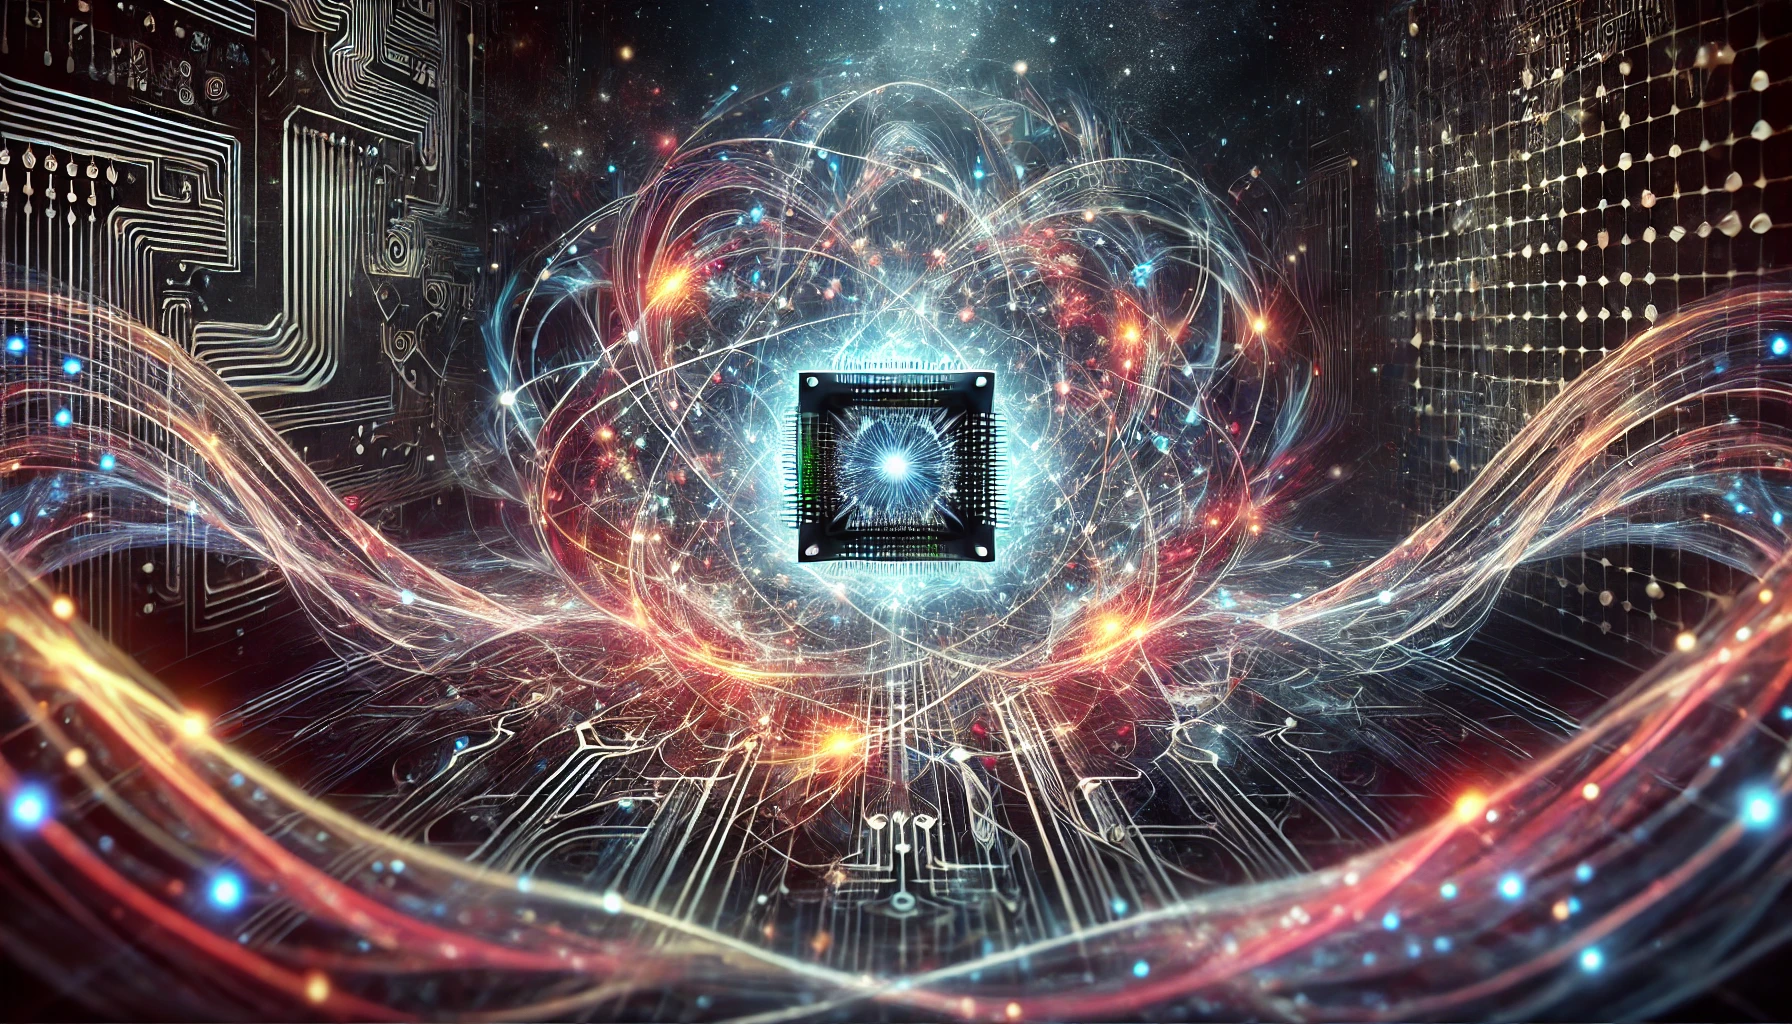
\includegraphics[width=0.8\textwidth]{quantum_computing.png}

    \caption{Quantum Computing}
\end{figure}

The challenge of maintaining quantum coherence across multiple scales illuminates crucial distinctions between quantum computing and conscious processing \cite{Terhal2018}. While quantum systems can achieve remarkable computational efficiency through coherent quantum states, these states remain inherently fragile and difficult to maintain at scales relevant to conscious processing. This fundamental limitation suggests that quantum computing may not provide direct insights into how consciousness emerges from physical systems \cite{Wallraff2021}.

Recent experimental achievements in quantum computing have demonstrated both the power and constraints of quantum approaches \cite{Zhong2020}. While quantum systems can solve certain problems with unprecedented efficiency, they must operate under highly controlled conditions that limit their ability to support the kind of adaptive, environment-interactive processing that characterizes consciousness \cite{Aaronson2021a}. This fundamental tension between computational power and environmental sensitivity suggests inherent limitations in applying quantum principles to conscious-like processing.

The role of decoherence in quantum systems takes on particular significance when considered through ECC's framework \cite{Arute2019}. Unlike conscious systems that maintain coherent processing through continuous interaction with their environment, quantum systems lose their coherent properties through environmental interaction. This fundamental difference suggests that quantum computing may operate in a fundamentally different regime than conscious processing \cite{Bernstein2018}.

The relationship between quantum and classical information processing reveals important insights about the nature of conscious computation \cite{Deutsch2020}. While quantum systems can perform certain calculations with remarkable efficiency, they cannot maintain the kind of stable, adaptive coherence that ECC identifies as crucial for consciousness. This limitation becomes particularly evident when considering how conscious systems maintain coherent processing while continuously interacting with their environment \cite{DiVincenzo2019}.

Quantum error correction and fault tolerance, while crucial for quantum computing, highlight fundamental differences from conscious processing \cite{Harrow2020}. The sophisticated mechanisms required to maintain quantum coherence contrast sharply with how biological systems achieve stable conscious processing through continuous interaction with their environment. This distinction suggests that conscious processing may operate through fundamentally different principles than quantum computation \cite{Kitaev2018}.

The theoretical foundations of quantum computing have revealed important insights about the nature of computation itself \cite{Montanaro2021}. However, these insights may be more relevant to understanding the fundamental limits of computation rather than providing direct mechanisms for implementing conscious-like processing. This suggests that advancing artificial consciousness might require focusing on classical-scale coherent dynamics rather than quantum effects \cite{Nielsen2020}.

The limitations of quantum computing in supporting conscious-like processing become particularly evident when considering the requirements for stable, adaptive behavior \cite{Preskill2019}. While quantum systems can achieve remarkable computational feats, they cannot maintain the kind of continuous, environment-interactive processing that characterizes consciousness. This fundamental limitation suggests that quantum computing may represent a powerful but ultimately distinct computational paradigm from conscious processing \cite{Shor2019}.

The relationship between quantum entanglement and conscious integration reveals important distinctions \cite{Svore2020}. While entanglement enables powerful quantum computations, it operates under fundamentally different principles than the classical-scale integration that characterizes conscious processing. The fragility of quantum entanglement contrasts sharply with the robust coherence maintained by conscious systems \cite{Terhal2018}.

Recent developments in quantum computing architecture have demonstrated both the potential and limitations of quantum approaches \cite{Wallraff2021}. While quantum systems continue to achieve impressive computational milestones, they remain fundamentally constrained by the need for extremely controlled environmental conditions. This requirement stands in stark contrast to how conscious systems maintain coherent processing while actively engaging with their environment \cite{Zhong2020}.

The distinction between quantum and classical coherence becomes particularly significant when considering the physical requirements for consciousness \cite{Aaronson2021a}. While quantum coherence enables powerful computational operations, ECC suggests that consciousness requires a different kind of coherence - one that operates at classical scales and remains stable through environmental interaction. This fundamental difference suggests that quantum computing, while revolutionary for certain computational tasks, may not directly advance our understanding of consciousness \cite{Arute2019}.

These considerations suggest that the future of artificial consciousness likely lies not in quantum computing but in systems capable of maintaining classical-scale coherent dynamics \cite{Bernstein2018}. While quantum computing will undoubtedly continue to advance and provide powerful computational capabilities, the development of conscious-like artificial systems may require focusing on different physical principles and architectural approaches \cite{Deutsch2020}.

The relationship between quantum computing and consciousness thus serves to illuminate important distinctions about the nature of conscious processing itself \cite{DiVincenzo2019}. Rather than requiring exotic quantum effects, consciousness may emerge from sophisticated classical-scale dynamics that enable stable, adaptive processing through continuous interaction with the environment. This understanding suggests new directions for developing artificial systems capable of supporting conscious-like processing while remaining grounded in classical physics.

\section{Alternative Forms of Computation}

Beyond the major paradigms of chemical and field computing, several specialized computational approaches demonstrate how information processing can emerge directly from physical dynamics rather than abstract symbol manipulation \cite{Adamatzky2021}. These alternative approaches illuminate important distinctions between abstract computation - which maintains strict isolation from physical processes - and concrete computation that remains embedded in physical dynamics.

Reservoir computing exemplifies "unsafe" computation by deliberately exploiting physical dynamics that resist complete formal specification \cite{Braund2020}. Unlike "safe" computation that enforces strict boundaries between program and effects, reservoir computing leverages the complex, nonlinear dynamics of physical systems directly. The reservoir's state space provides computational capacity through its intrinsic evolution rather than through controlled symbolic manipulation. This demonstrates how computation can emerge from physical dynamics that remain partially opaque to formal analysis.

The emerging field of natural computing provides particular insight into how physical systems can achieve sophisticated information processing without requiring digital abstraction \cite{Calude2018a}. These approaches demonstrate how computation can emerge directly from physical dynamics, suggesting new possibilities for developing systems capable of supporting conscious-like processing. This aligns with recent theoretical work examining how purposive behavior can emerge from physical systems without requiring explicit computational control \cite{Deacon2019}.

Chemical excitation waves represent another promising direction for alternative computation \cite{Gorecki2020}. These systems demonstrate how information processing can emerge from reaction-diffusion dynamics without requiring discrete state transitions. The continuous nature of chemical wave propagation provides mechanisms for implementing computation through physical processes that maintain direct connection to energy dynamics.

Recent advances in reservoir computing have demonstrated remarkable capabilities in processing temporal information through physical dynamics \cite{Jaeger2021}. Rather than implementing explicit computational architectures, these systems achieve sophisticated processing through the natural dynamics of physical systems. This approach suggests new possibilities for developing artificial systems that maintain closer alignment with how biological systems process information.

Enzyme-based logic systems provide concrete examples of how computation can emerge from molecular interactions \cite{Katz2019}. These systems demonstrate how sophisticated information processing can be achieved through natural biochemical processes rather than requiring implementation through artificial digital circuits. The success of these approaches suggests promising directions for developing new computational paradigms that maintain closer connection to physical dynamics.

These alternative computational approaches collectively demonstrate that information processing need not be restricted to the discrete, symbol-manipulating framework that has dominated computer science \cite{Levin2018}. From reservoir computing's exploitation of physical dynamics to enzyme-based logic systems, these approaches show how computation can remain grounded in continuous physical processes while achieving sophisticated information processing capabilities.

Emerging approaches to hybrid nanocomputing demonstrate how different computational paradigms might be integrated while maintaining connection to physical dynamics \cite{Mayne2019}. Rather than relying solely on digital or quantum approaches, these systems combine multiple computational mechanisms to achieve more sophisticated processing capabilities. This integration suggests new possibilities for developing systems that better align with how biological systems process information.

The study of biological computation through organisms like Physarum has revealed sophisticated information processing capabilities emerging from natural physical dynamics \cite{Nakagaki2020}. These systems demonstrate how computation can arise from the intrinsic properties of living systems without requiring explicit computational architecture. Such examples provide crucial insights into how conscious-like processing might emerge from physical systems.

Recent work in computational matter has demonstrated how information processing capabilities can emerge from material properties themselves \cite{Stepney2018}. Rather than imposing computation through external design, these approaches show how computational capabilities can arise from the inherent dynamics of physical systems. This perspective aligns with ECC's emphasis on the inseparability of conscious processing from its physical substrate.

DNA computing and molecular programming represent another significant direction in alternative computation \cite{Tanaka2021}. These approaches demonstrate how biological molecules can implement sophisticated computational operations through their natural interaction dynamics. The success of these systems suggests new possibilities for developing computational architectures that maintain closer connection to biological information processing.

The relationship between physics and computation takes on particular significance when considering these alternative approaches \cite{Toffoli2019}. Rather than treating physical implementation as secondary to logical structure, these systems demonstrate how computational capabilities can emerge directly from physical dynamics. This perspective helps clarify how conscious systems might achieve sophisticated information processing through natural physical processes.

Molecular computing based on the lock-key paradigm provides another example of how computation can emerge from physical interactions \cite{Zauner2020}. These systems achieve information processing through molecular recognition and binding, demonstrating how computation can be implemented through natural physical processes rather than requiring artificial digital circuits. Such approaches suggest new directions for developing computational systems that maintain closer alignment with biological information processing.

The implications of these alternative computational approaches extend beyond theoretical interest to practical questions about developing artificial conscious systems \cite{Calude2018a}. Rather than attempting to achieve consciousness through traditional digital architectures, these approaches suggest new possibilities for developing systems that maintain closer connection to the physical dynamics that characterize biological consciousness \cite{Deacon2019}.

Recent advances in unconventional computing have demonstrated how different computational paradigms might be combined to achieve more sophisticated processing capabilities \cite{Gorecki2020}. The integration of multiple approaches - from chemical computing to field-based systems - suggests new possibilities for developing artificial systems capable of supporting the kind of coherent processing that consciousness requires \cite{Jaeger2021}.

The relationship between physical implementation and computational capability becomes particularly significant when considering these alternative approaches \cite{Katz2019}. Unlike traditional digital systems that abstract away from physical details, these alternative computational paradigms demonstrate how sophisticated information processing can emerge directly from physical dynamics. This perspective aligns with ECC's emphasis on the inseparability of conscious processing from its physical substrate \cite{Levin2018}.

The success of biological computing systems in achieving sophisticated information processing through natural physical processes suggests important directions for future research \cite{Mayne2019}. Rather than imposing computational structure through external design, these systems demonstrate how computation can emerge from the intrinsic properties of physical systems. This approach suggests new possibilities for developing artificial systems that better mirror how biological systems achieve conscious processing \cite{Nakagaki2020}.

Looking forward, the development of artificial conscious systems might require synthesizing insights from multiple alternative computational approaches \cite{Stepney2018}. Rather than relying on any single paradigm, future systems might need to integrate multiple computational mechanisms while maintaining close connection to physical dynamics. This integration could provide practical paths toward developing artificial systems capable of supporting genuine conscious-like processing \cite{Toffoli2019}.

These considerations suggest that advancing artificial consciousness might require fundamentally rethinking our approach to computation itself \cite{Zauner2020}. Rather than treating computation as abstract symbol manipulation, we might need to develop new paradigms that maintain closer connection to the physical dynamics that characterize biological consciousness. Such approaches could provide crucial insights into how conscious processing emerges from physical systems while suggesting new directions for developing artificial conscious systems.

\section{(In)finite Algorithms}

The classical theory of computation, emerging from seminal work on effective procedures and mechanical calculation, established computation as fundamentally tied to finite algorithmic processes \cite{Davis2000}. However, recent theoretical developments suggest that understanding consciousness may require moving beyond traditional notions of finite algorithms to consider computational processes that transcend classical boundaries \cite{Downey2010}.

The standard notion of computation assumes that while program execution may continue indefinitely through loops or recursion, the underlying instruction set must remain finite \cite{Rogers1987}. This constraint emerges from both practical and theoretical considerations - physical computers must store programs in finite memory, and formal systems like the Lambda Calculus operate with finite sets of rules and symbols \cite{Barendregt1984}. Even universal Turing machines, despite their infinite tape, employ finite sets of states and transition rules.

However, theoretical exploration of infinite algorithmic processes suggests intriguing possibilities at the boundaries of classical computation \cite{Hamkins2014}. Stream-based models and lazy evaluation in functional programming paradigms allow for potentially infinite data structures, though the programs manipulating them remain finite. Self-modifying code and recursive self-improvement systems can generate new instructions during runtime, creating the appearance of infinite programs through continuous expansion \cite{Goldin2006}.

Higher-order logics and proof theory provide frameworks for reasoning about infinite computational processes \cite{Mancosu2008}. Infinite proofs in $\omega$-logic and coinductive reasoning demonstrate how we might conceptualize valid infinite computational processes, even if they cannot be directly implemented in classical machines \cite{Boolos2007}. These theoretical constructs suggest ways that computational processes might transcend finite bounds while maintaining logical coherence.

The relationship between finite algorithms and consciousness raises profound theoretical questions \cite{Hofstadter1999}. If consciousness emerges from processes that cannot be reduced to finite algorithms, this would suggest fundamental limitations in computational theories of mind. ECC proposes that consciousness requires continuous, field-like processes that may be better understood through infinite or continuous mathematical frameworks rather than discrete, finite computational models \cite{Floyd2014}.

Moreover, the distinction between finite and infinite algorithmic processes illuminates key differences between digital computation and biological consciousness \cite{Kozen2006}. Where digital computers operate through finite state transitions, conscious systems maintain continuous fields of coherent energy that may be better modeled through infinite or continuous processes. This suggests that consciousness may require frameworks that transcend classical computational limitations.

The relationship between finite algorithms and continuous physical processes takes on particular significance when considering consciousness \cite{PourEl1989}. While finite algorithms can simulate aspects of continuous dynamics, they fundamentally cannot capture the kind of seamless, unbroken processing that characterizes conscious experience. This limitation suggests that understanding consciousness may require moving beyond traditional computational paradigms \cite{Sipser2012}.

The question of infinite algorithms becomes especially relevant when examining how nature implements computation-like processes \cite{Soare2016}. Biological systems, particularly cells, demonstrate sophisticated information processing capabilities that transcend traditional notions of finite algorithmic steps. These natural computing processes suggest ways that infinite or continuous computation might be physically realized while maintaining coherent organization \cite{vanLeeuwen2012}.

DNA represents a particularly sophisticated example of natural computation that challenges traditional algorithmic boundaries \cite{Wegner2003}. Unlike finite programs with fixed instruction sets, DNA functions as a self-updating metaprogram that evolves and modifies itself over time. This dynamic computational system demonstrates how biological processes can implement sophisticated information processing without requiring finite algorithmic specification \cite{Deutsch2011}.

The cell itself functions as a kind of natural computer that processes information through continuous molecular interactions rather than discrete logic gates \cite{Rovelli2018}. Cellular computation demonstrates several key properties that distinguish it from classical finite algorithms: continuous parallel processing across multiple chemical pathways, integration of information processing with physical energy flows, and dynamic modification of computational architecture \cite{Aaronson2013}.

These biological implementations of computation suggest fundamental limitations in traditional algorithmic approaches \cite{Copeland2004}. Rather than operating through finite sets of instructions, biological systems achieve sophisticated information processing through continuous physical processes that maintain coherent organization across multiple scales. This perspective aligns with ECC's emphasis on consciousness as emerging from continuous, physically-grounded processes rather than discrete computational steps.

The implications for artificial consciousness are profound \cite{Rogers1987}. If consciousness emerges from biological processes that implement continuous rather than discrete computation, this suggests fundamental limitations in classical computational approaches to mind. Understanding consciousness may require frameworks that can bridge discrete algorithmic processes with continuous physical dynamics.

The study of infinite algorithms points toward deeper questions about the nature of computation itself and its relationship to physical processes \cite{Hamkins2014}. Rather than remaining within the confines of classical computer science, we must consider how natural systems implement sophisticated information processing through continuous, physically-grounded processes. This may lead to new paradigms that transcend traditional notions of finite and infinite algorithms while remaining grounded in physical reality \cite{Sipser2012}.

These insights about natural computing and infinite-like processes point toward fundamental limitations in discrete digital computation \cite{Wegner2003}. While digital systems must ultimately reduce all operations to finite sets of binary instructions, nature implements sophisticated information processing through continuous physical processes. This distinction becomes particularly crucial when considering consciousness, which appears to require the kind of continuous, field-like properties that digital computation cannot easily replicate \cite{PourEl1989}.

The implementation of apparently infinite processes in biological systems suggests that the key distinction may not be between finite and infinite algorithms, but between discrete and continuous modes of computation \cite{Goldin2006}. Biological systems achieve sophisticated information processing without requiring either finite instruction sets or infinite storage. Instead, they maintain coherent organization through continuous energy flows and dynamic feedback loops that operate across multiple scales simultaneously \cite{Floyd2014}.

This perspective suggests that consciousness may emerge from processes that are neither strictly finite nor infinite in the classical computational sense, but rather continuous and field-like in nature \cite{Barendregt1984}. The brain does not implement either a finite or infinite algorithm, but rather maintains coherent energy states through continuous physical processes that enable conscious experience to emerge \cite{Boolos2007}.

The limitations of classical computational approaches become particularly evident when considering how biological systems integrate information processing with physical energy flows \cite{Kozen2006}. Unlike digital computers that must maintain strict separation between information and physical implementation, biological systems achieve sophisticated computation precisely through their physical organization and energy dynamics \cite{Mancosu2008}.

\newpage
\section{References}
\printbibliography[title={},heading=subbibliography]
%\printbibliography[title={References: Artificial Systems}]
\end{refsection}

\section*{\phantom{Part IX Comparative Analysis}}
\h{Comparative Analysis}

\begin{refsection}[references/0001_6_other_theories.bib]

Energetically Coherent Computation (ECC) exists in complex dialogue with established theories of consciousness, offering both convergences and significant departures. The framework provides a distinctive physical grounding that reshapes our conceptualization of conscious experience while engaging with key insights from major theoretical approaches.

The relationship between ECC and Integrated Information Theory (IIT) proves particularly instructive. Where IIT posits that consciousness emerges from integrated information with high $\Phi$ values \cite{Koch2018}, ECC suggests consciousness arises from coherent energy flows within physical substrates. While both theories emphasize unity and integration, they propose fundamentally different mechanisms. IIT focuses on abstract information integration independent of physical substrate, while ECC emphasizes physically grounded energy dynamics and coherence patterns. This distinction carries significant implications for artificial consciousness - while IIT suggests consciousness could emerge in any system with sufficient information integration, ECC requires specific physical conditions and energy dynamics.

Global Workspace Theory (GWT) similarly finds both resonance and tension with ECC. While GWT describes consciousness as information gaining access to a "global workspace" for widespread broadcasting \cite{Baars2019}, ECC frames consciousness as emerging from coherent energy fields. Where GWT focuses on information access and distribution, ECC examines the underlying field dynamics that enable global integration. This shifts the emphasis from discrete broadcasting to continuous coherence maintenance.

Higher Order Theories (HOT) posit that consciousness requires higher-order representations of mental states \cite{Block2020}. ECC contrasts sharply with this view by suggesting consciousness emerges directly from coherent energy dynamics. Rather than requiring meta-representations, ECC grounds consciousness in base-level energy coherence. This reflects a fundamental difference in how the theories conceptualize the architecture of conscious experience.

The predictive processing framework finds interesting parallel developments with ECC, though through different mechanisms \cite{Clark2019}. While predictive processing uses abstract Bayesian inference hierarchies, ECC examines concrete energy dynamics. Both theories emphasize self-organization, but ECC grounds this organization in physical energy flows rather than abstract prediction error minimization \cite{Friston2020}.

This comparative analysis reveals ECC as offering a distinct perspective that emphasizes physical grounding while engaging with key insights from other theories. By examining how patterns of energetic coherence relate to established theoretical frameworks, ECC suggests new ways to understand both the possibilities and limitations of conscious systems. The framework's emphasis on physical grounding opens new avenues for empirical investigation while maintaining productive dialogue with existing theoretical approaches.

A fundamental distinction emerges when examining how most theories of consciousness tacitly adopt computationalist assumptions \cite{Chalmers2018}. Even theories that seem to move beyond pure computation - like IIT or GWT - often retain an underlying commitment to treating consciousness as fundamentally computational. ECC breaks from this tradition by suggesting that consciousness emerges from physical energy dynamics that cannot be reduced to computation alone.

The fundamental distinctions between various theories of consciousness become particularly evident when examining their treatment of empirical findings. Global Workspace Theory describes consciousness through the metaphor of a computational theater where different processors compete for access \cite{Baars2019}. While this model captures important aspects of conscious access, it remains fundamentally computational in its architecture. ECC suggests instead that what appears as competition for conscious access actually reflects competition between different patterns of energetic coherence, grounded in physical rather than computational dynamics.

Similarly, predictive processing frameworks typically describe hierarchical prediction using the language of Bayesian computation, even when emphasizing embodied aspects of cognition \cite{Clark2019}. ECC reconceptualizes prediction not as computational Bayesian inference but as emerging from stable patterns of energetic coherence that naturally anticipate future states through their physical dynamics. This shifts the theoretical foundation from abstract probability distributions to concrete energy flows \cite{Friston2020}.

Higher Order Theories, despite moving beyond simple computation by introducing meta-representational requirements \cite{Block2020}, still generally assume these representations operate through computational mechanisms. ECC suggests instead that any metacognitive capacities emerge from specific patterns of energetic coherence rather than computational hierarchies. This grounds higher-order awareness in physical dynamics rather than abstract computation.

Even Integrated Information Theory, while breaking important ground in linking consciousness to physical systems \cite{Koch2018}, retains computational assumptions in how it quantifies integration through mathematical information theory. ECC suggests that integration emerges not from abstract information processing but from actual patterns of energetic coherence maintained through biological mechanisms \cite{Tononi2021}.

The persistence of computationalist assumptions across theories of consciousness reflects the powerful influence of the computational metaphor in cognitive science. However, this reliance on computation may ultimately limit our understanding of consciousness. ECC suggests that consciousness requires specific forms of physical organization that cannot be captured through computational models alone \cite{Dehaene2021}.

This insight carries significant implications for artificial consciousness. Where computationalist theories suggest consciousness could emerge from sufficient computational complexity, ECC indicates that conscious machines would require specific physical architectures capable of maintaining coherent energy dynamics similar to biological systems. This provides clearer constraints on what types of systems could potentially support consciousness while suggesting new directions for artificial consciousness research beyond traditional computational approaches.

By grounding consciousness in energetic coherence rather than computation, ECC offers a framework for understanding features of conscious experience that prove difficult to explain computationally - from the unity of consciousness to the qualitative richness of experience \cite{Lamme2020}. This suggests that progress in understanding consciousness may require moving beyond computational paradigms to examine the underlying physical dynamics that make conscious experience possible.

This theoretical reframing helps resolve longstanding philosophical issues like the symbol grounding problem more directly. Rather than attempting to connect abstract symbols to meaning through computational processes, ECC suggests how meaning emerges naturally from patterns of energetic coherence grounded in physical reality. This provides a more fundamental basis for understanding how conscious systems achieve genuine intentionality and semantic content \cite{Chalmers2018}.

The embodied and phenomenological dimensions of consciousness take on particular significance when examined through ECC's framework. While traditional cognitive science often treats embodiment as an implementation detail, the enactive approach developed in foundational work emphasizes how consciousness emerges from the dynamic coupling between organism and environment \cite{Varela2017}. ECC strengthens this perspective by providing concrete physical mechanisms through which such coupling occurs via patterns of energetic coherence.

The relationship between consciousness and biological processes finds sophisticated treatment in recent theoretical developments \cite{Thompson2018}. Rather than treating biological implementation as incidental to conscious processing, ECC suggests that specific biological mechanisms enable the particular forms of energetic coherence necessary for consciousness. This aligns with emerging perspectives that emphasize the deep continuity between life and mind while providing physical mechanisms to explain this connection.

Recent work on the predictive aspects of conscious experience has suggested important links between perception, action, and conscious awareness \cite{Seth2021}. ECC reframes these predictive relationships not as computational processes but as emerging naturally from the physical dynamics of coherent energy fields. This provides a more fundamental basis for understanding how conscious systems achieve the anticipatory capabilities emphasized in contemporary theories.

The electromagnetic field theory of consciousness offers interesting parallels with ECC's framework \cite{McFadden2020}. While both approaches emphasize field-like properties of conscious experience, ECC suggests that electromagnetic fields represent just one aspect of the broader patterns of energetic coherence necessary for consciousness. This more comprehensive view helps explain how different physical mechanisms integrate to create unified conscious experience.

Higher-order theories of consciousness have proposed sophisticated models of how self-awareness emerges through metacognitive representation \cite{Rosenthal2019}. ECC suggests instead that self-awareness emerges naturally from recursive patterns of energetic coherence without requiring explicit meta-representation. This provides a more parsimonious account of how conscious systems achieve self-awareness while maintaining closer contact with physical dynamics.

This synthesis reveals ECC as offering a distinctive theoretical framework that engages productively with existing theories while suggesting new directions for consciousness research. By grounding conscious experience in patterns of energetic coherence rather than abstract computation or pure phenomenology, ECC provides concrete mechanisms that help bridge traditional divides between physical and experiential approaches to consciousness. This theoretical integration suggests promising directions for future empirical investigation while maintaining rigorous connection to both physical and phenomenological aspects of conscious experience.
     
\section{IIT and Panpsychism}

%TODO: this section is quite repetitive

The relationship between Energetically Coherent Computation (ECC) and both Integrated Information Theory (IIT) and panpsychist approaches reveals important theoretical convergences while maintaining distinct positions on consciousness's physical basis. Where IIT posits consciousness as identical to integrated information \cite{Tononi2008}, and panpsychism suggests consciousness pervades all matter \cite{Strawson2006}, ECC frames consciousness as emerging from specific patterns of energetic coherence within biological systems.

At its core, IIT offers a mathematical framework for quantifying consciousness through integrated information ($\Phi$) \cite{Tononi2016}. While ECC appreciates IIT's attempt to provide rigorous measures of consciousness, it suggests that integration emerges from physical energy dynamics rather than abstract information processing. This distinction proves crucial - where IIT remains largely substrate-independent, ECC insists on specific physical requirements through energetic coherence and field dynamics. The rich alphabet requirement in ECC, shaped by transcriptomic profiles and cellular organization, provides concrete constraints on possible implementations of consciousness that go beyond IIT's more abstract specifications.

ECC aligns with panpsychism in rejecting purely computational approaches to consciousness and emphasizing its grounding in physical reality \cite{Nagel1979}. However, where panpsychism attributes consciousness to all matter, ECC suggests consciousness requires specific forms of energetic coherence typically found only in biological systems. This more restricted view helps avoid the combination problem that plagues panpsychist accounts \cite{Chalmers2015} - how simple forms of consciousness combine into complex experiences. ECC explains this through its framework of coherent energy dynamics and field integration.

The theories also differ in their treatment of emergence \cite{Goff2019}. Panpsychism often posits consciousness as fundamental, while IIT suggests it emerges from information integration \cite{Oizumi2014}. ECC charts a middle path, proposing that consciousness emerges from specific patterns of energetic coherence while remaining irreducibly physical. This approach maintains connection to physical reality while explaining why consciousness appears only in certain types of organized systems.

Particularly significant is how ECC addresses the explanatory gap between physical processes and conscious experience \cite{Koch2019}. Rather than making consciousness ubiquitous like panpsychism or reducing it to information like IIT, ECC suggests how specific patterns of energetic coherence give rise to conscious experiences through their inherent physical dynamics. This provides a more concrete basis for understanding both the emergence of consciousness and its qualitative features.

The historical development of panpsychist thought in Western philosophy \cite{Skrbina2017} reveals persistent tensions that ECC's framework helps address. While panpsychism attempts to solve the hard problem by making consciousness fundamental to all matter, and IIT seeks to bridge the explanatory gap through information theory \cite{Tononi2015}, ECC suggests that the qualitative aspects of consciousness emerge naturally from specific patterns of energetic coherence, providing a physical basis for phenomenal experience without reducing it to computation or making it universal.

This theoretical synthesis suggests ECC might help bridge aspects of IIT and panpsychism while maintaining its distinctive emphasis on physical energy dynamics. By grounding consciousness in specific patterns of energetic coherence, ECC provides a framework that acknowledges both the physical basis of consciousness and its emergence in complex biological systems, while avoiding the metaphysical challenges that have historically plagued both panpsychist and purely informational approaches \cite{Shani2015}.

The dynamic core hypothesis, developed before IIT, provides an important historical bridge between neural integration theories and ECC's framework. Where the dynamic core hypothesis proposed that consciousness emerges from integrated neural activity in thalamocortical systems, ECC extends this insight by specifying how such integration occurs through coherent energy dynamics. Both approaches emphasize the importance of dynamic integration \cite{Tononi2008}, but ECC grounds this integration in physical field effects rather than purely neural computation.

Particularly relevant is how the dynamic core hypothesis identified the importance of rapid neural integration and differentiation. ECC builds on this insight by explaining how such integration occurs through field-like properties of energetic coherence, maintained through astrocytic networks and the extracellular matrix. This provides a physical mechanism for the kind of dynamic integration that early IIT described primarily in computational terms \cite{Oizumi2014}.

The progression from dynamic core to IIT to ECC reveals an interesting theoretical evolution. The dynamic core hypothesis began with biological neural systems, IIT abstracted these principles into substrate-independent information integration \cite{Tononi2015}, and ECC returns to physical implementation while maintaining mathematical rigor through its sheaf-theoretic framework and stress-energy tensor formalism.

This theoretical progression also illuminates key differences in how these frameworks approach the hard problem of consciousness \cite{Chalmers2015}. Panpsychism attempts to dissolve the hard problem by making consciousness fundamental to all matter \cite{Strawson2006}. IIT seeks to bridge the explanatory gap through information theory. ECC suggests instead that the qualitative aspects of consciousness emerge naturally from specific patterns of energetic coherence, providing a physical basis for phenomenal experience without reducing it to computation or making it universal.

The relationship between these theories has important implications for understanding both biological and artificial consciousness \cite{Koch2019}. Where IIT opened the possibility of non-biological consciousness through information integration, ECC suggests more specific requirements based on energetic coherence. This provides clearer constraints on what types of systems could potentially support consciousness while explaining why biological systems prove particularly suited to generating conscious experience.

These theoretical relationships also help clarify how consciousness might have evolved \cite{Goff2019}. Rather than consciousness being either fundamental (panpsychism) or emerging suddenly through sufficient information integration (IIT), ECC suggests a gradual evolution of increasingly sophisticated patterns of energetic coherence in biological systems. This aligns with recent research in cellular cognition and basal awareness while explaining how more complex forms of consciousness emerged \cite{Mathews2011}.

IIT's relationship to panpsychism emerges from its fundamental premise that consciousness is identical to integrated information \cite{Tononi2016}. Since information integration exists to some degree in all physical systems, IIT leads naturally toward a panpsychist view where consciousness exists ubiquitously, though in varying degrees. This marks a crucial difference from ECC, which identifies consciousness with specific patterns of energetic coherence rather than information integration per se.

This tendency toward panpsychism represents both a strength and limitation of IIT \cite{Tononi2008}. While it provides a unified theoretical framework, it struggles to explain why consciousness appears limited to certain types of systems and how simple forms of consciousness combine into complex experiences \cite{Chalmers2015}. ECC addresses these challenges by specifying physical requirements for consciousness through energetic coherence, transcriptomic profiles, and field dynamics.

The progression from early work on the dynamic core to IIT's more abstract formulation reveals an interesting theoretical trajectory \cite{Tononi2016}. Where the dynamic core hypothesis began with concrete neural mechanisms, IIT moved toward increasingly mathematical and substrate-independent descriptions. ECC suggests a return to physical implementation while maintaining mathematical rigor through its sheaf-theoretic framework and field dynamics.

Recent developments in panpsychist thought \cite{Skrbina2017} have attempted to address the combination problem through various theoretical innovations. However, these solutions often remain abstract and disconnected from biological reality. ECC's framework offers a more concrete approach by showing how physical patterns of energetic coherence naturally combine and integrate across scales without requiring additional metaphysical principles.

The cosmological implications of panpsychism \cite{Shani2015} raise important questions about the relationship between consciousness and fundamental physical processes. While ECC shares with panpsychism an emphasis on the physical basis of consciousness, it suggests that conscious experience requires specific forms of organized complexity rather than being inherent in all matter. This provides a clearer explanation for why consciousness appears in some systems but not others.

IIT's mathematical formalization of consciousness \cite{Oizumi2014} represents an important attempt to quantify conscious experience. However, its focus on information integration independent of physical implementation may miss crucial aspects of how consciousness actually emerges in biological systems. ECC maintains the mathematical rigor of IIT while grounding it more firmly in physical reality through its analysis of energetic coherence patterns.

The fundamental tension between panpsychist and emergentist approaches to consciousness \cite{Goff2019} finds potential resolution through ECC's framework. Rather than choosing between consciousness as fundamental or as purely emergent, ECC suggests how specific patterns of physical organization give rise to conscious experience through their inherent dynamics. This provides a middle path between panpsychist and emergentist extremes while maintaining clear connection to empirical investigation.

This theoretical synthesis suggests productive new directions for consciousness research that move beyond both pure computation and simple panpsychism \cite{Koch2019}. By examining how specific patterns of energetic coherence support conscious experience, we may develop more sophisticated understanding of both the physical basis of consciousness and its qualitative features. This approach maintains rigorous connection to physical reality while acknowledging the irreducible aspects of conscious experience that have motivated panpsychist approaches.

ECC and IIT share conceptual territory in their emphasis on integration as a fundamental property of conscious systems, though they differ markedly in their metaphysical commitments and explanatory frameworks \cite{Tononi2008}. 

A primary distinction lies in their treatment of physical implementation. ECC positions energy flows as foundational, viewing consciousness as emerging from coherent organization of energy across physical modalities - electromagnetic, chemical, and mechanical. This stands in contrast to IIT's more abstract approach, which, while acknowledging physical substrates, focuses primarily on informational integration and causal structures \cite{Tononi2016}. Where ECC rejects hardware-software distinctions as fundamental, IIT abstracts consciousness into mathematical frameworks independent of specific energetic dynamics.

The theories also diverge in their treatment of integration versus coherence. IIT defines consciousness through $\Phi$, a quantitative measure of integrated information that captures how irreducible a system's causal structure is to its constituent parts \cite{Oizumi2014}. ECC, conversely, emphasizes coherence grounded in energetic dynamics rather than pure information. This coherence encompasses energetic efficiency, field stability, and specific physical substrate requirements that extend beyond informational integration.

A further crucial distinction lies in their treatment of phenomenology. ECC positions phenomenal experience as directly emergent from physical energy patterns, while IIT approaches phenomenology through the mathematical quantification of integrated information \cite{Tononi2015}. This reflects a deeper philosophical divergence - where IIT maintains a degree of substrate independence that aligns with certain panpsychist interpretations \cite{Koch2019}, ECC insists on specific physical implementations that respect energetic coherence.

The ontological commitments of these frameworks reveal fundamentally different approaches to consciousness. IIT's mathematical formalization of consciousness as integrated information suggests alignment with broader panpsychist traditions \cite{Chalmers2015}, while ECC's insistence on specific physical dynamics positions it closer to biological naturalism. These distinct metaphysical foundations shape how each theory approaches key questions in consciousness research, from the hard problem to the possibility of machine consciousness.

This analysis reveals not just theoretical differences but fundamentally distinct research programs. Where IIT directs attention toward mathematical formalization of information integration, ECC emphasizes investigation of physical energy dynamics in biological systems. These divergent approaches suggest different experimental priorities and methodological commitments in consciousness research.

Through this comparative lens, we see how ECC and IIT represent distinct paradigms in consciousness research, each offering unique insights while maintaining different relationships to the physical implementation of conscious experience. Their contrasting approaches to physical substrates, integration, and phenomenology illuminate crucial questions about the nature of consciousness and its relationship to physical reality.

The ontological distinctions between ECC and IIT reflect broader debates in consciousness studies about the relationship between physical implementation and mental phenomena \cite{Nagel1979}. Where ECC grounds consciousness in physical energy dynamics, IIT's more abstract informational framework aligns with certain strands of computational theory of mind while maintaining unique metaphysical commitments \cite{Tononi2016}.

ECC's physicalist ontology positions energy flows as the fundamental constituents of both physical reality and consciousness. This approach emphasizes direct causation through electromagnetic, chemical, and thermal dynamics, rejecting abstractions that separate computational description from physical implementation. The theory suggests that specific perturbations in energy flows correspond directly to changes in phenomenal experience, making concrete predictions about the relationship between physical dynamics and conscious states \cite{Koch2019}.

In contrast, IIT operates from an informational ontology where consciousness emerges from specific patterns of integrated information, quantified through $\Phi$ \cite{Oizumi2014}. This framework treats information structures and their causal relationships as primary, allowing for substrate independence in principle. While acknowledging the need for physical implementation, IIT positions the mathematical structure of information integration as the essential feature of consciousness.

These distinct ontological commitments shape how each theory approaches the relationship between brain and consciousness. ECC's emphasis on specific physical dynamics aligns with certain aspects of naturalistic approaches \cite{Goff2019}, while suggesting that consciousness requires particular forms of energetic coherence that cannot be reduced to abstract computation. IIT's more abstract framework, while mathematically sophisticated, raises questions about the relationship between information, causation, and physical implementation \cite{Tononi2015}.

The theories' divergent approaches to substrate independence particularly illuminate their philosophical differences. ECC's insistence on specific physical implementation suggests that consciousness cannot be realized in arbitrary substrates, even if they implement similar computational structures. This contrasts with IIT's more permissive view regarding physical implementation, though both theories maintain sophisticated accounts of how consciousness relates to physical systems \cite{Strawson2006}.

These ontological distinctions carry significant implications for consciousness research. ECC directs attention toward investigating specific physical mechanisms and energy dynamics in biological systems, while IIT emphasizes mathematical modeling of information integration. Both approaches contribute valuable insights while suggesting different experimental priorities and methodological commitments in the study of consciousness.

The contrast between energetic and informational ontologies also raises important questions about the nature of causation in conscious systems. ECC's emphasis on physical energy flows suggests direct causal relationships between neural dynamics and conscious experience, while IIT's focus on informational integration provides a different perspective on mental causation \cite{Tononi2008}. These different approaches to causation reflect broader philosophical debates about the relationship between physical and mental phenomena.

Through careful examination of these ontological commitments, we gain deeper insight into how different theoretical frameworks approach the challenge of explaining consciousness. The contrast between ECC and IIT illuminates crucial questions about the relationship between physical implementation, information processing, and conscious experience.

The philosophical implications of these contrasting frameworks extend beyond theoretical distinctions to fundamental questions about the nature of consciousness and its place in physical reality \cite{Skrbina2017}. ECC's energetic monism suggests a unified view where energy serves as the foundational substance underlying both physical and phenomenal properties. This perspective aligns with certain naturalistic approaches while maintaining distinct claims about the specific physical requirements for consciousness.

IIT's framework, in contrast, suggests what might be termed an informational dual-aspect theory, where information possesses both physical and experiential aspects \cite{Tononi2016}. This approach shares certain features with panpsychist perspectives while maintaining its unique emphasis on integrated information as the basis for consciousness \cite{Mathews2011}. The theory's mathematical formalization of consciousness through $\Phi$ suggests a kind of pan-computationalism, though with specific requirements for information integration that distinguish it from simpler computational theories.

These distinct philosophical commitments shape how each theory approaches key questions in consciousness research. ECC's emphasis on physical dynamics suggests that understanding consciousness requires detailed investigation of energy flows in biological systems, particularly focusing on electromagnetic fields and chemical gradients in neural tissue. IIT, conversely, directs attention toward developing increasingly sophisticated mathematical models of information integration \cite{Oizumi2014}.

The theories also differ in their predictions about artificial consciousness. ECC's insistence on specific physical implementation suggests strict constraints on what types of systems could potentially support consciousness, requiring particular forms of energetic coherence typically found in biological systems. IIT's more abstract framework allows for the possibility of conscious artificial systems, provided they achieve sufficient levels of integrated information \cite{Koch2019}.

The relationship between phenomenology and physical implementation represents another crucial distinction. ECC suggests that conscious experience emerges directly from patterns of energetic coherence, making specific predictions about how physical perturbations should correspond to changes in phenomenal experience. IIT approaches phenomenology through mathematical formalization of information structures, suggesting different experimental approaches to investigating conscious experience \cite{Shani2015}.

These theoretical distinctions carry significant implications for the future of consciousness research. Where ECC suggests focusing on physical mechanisms and energy dynamics in biological systems, IIT points toward mathematical modeling and quantification of information integration. Both approaches offer valuable insights while maintaining different relationships to the hard problem of consciousness \cite{Goff2019}.

Through careful analysis of these theoretical frameworks, we gain deeper insight into the challenges and opportunities in consciousness research. The contrast between ECC and IIT illuminates crucial questions about the nature of consciousness, its relationship to physical reality, and the prospects for developing a comprehensive scientific understanding of conscious experience.

\begin{table}[h!]
\centering
\setlength{\extrarowheight}{2pt} % Adds extra row height for readability
\begin{tabularx}{\textwidth}{@{}p{3cm}Xp{4cm}@{}}
\toprule
\textbf{Aspect} & \textbf{ECC: Energy Ontology} & \textbf{IIT: Information Ontology} \\ \midrule
\textbf{Primary Basis} & Energy and its physical flows & Information and its causal structure \\
\textbf{Relation to Consciousness} & Arises from coherent energy flows across physical modalities (e.g., electromagnetic, chemical) & Arises from integrated information ($\Phi$), quantified as the irreducibility of causal interactions \\
\textbf{Role of Physicality} & Physical energy flows are fundamental; no abstraction between hardware and software & Physical implementation is secondary; causal informational structure is primary \\
\textbf{Phenomenology} & Grounded in energy patterns and their dynamic organization; directly tied to physical energy flows & Grounded in abstract informational integration; explained through the mathematical structure of $\Phi$ \\
\textbf{Substrate Dependence} & Substrate-specific: requires physical systems capable of coherent energy organization (e.g., EM fields in neurons) & Substrate-independent: any system with sufficient integrated causal structures \\
\textbf{Core Mechanism} & Coherence of energy dynamics enabling integration and efficiency in physical systems & Irreducible integration of information as measured by $\Phi$ \\
\textbf{Richness of Representation} & Based on a rich alphabet of energy flows (e.g., electromagnetic, chemical) to form high-dimensional states & Based on binary or abstract informational states, emphasizing causal interaction \\
\textbf{Research Direction} & Physical energy dynamics in the brain (e.g., EM fields and ion flows) & Models of informational integration and causal structures \\
\textbf{Philosophical Alignment} & Energetic monism: energy as the unifying substance of conscious and physical phenomena & Dual-aspect theory or pancomputationalism: information as the fundamental basis for consciousness \\ \bottomrule
\end{tabularx}
\caption{Energetically Coherent Computation (ECC) and Integrated Information Theory (IIT)}
\label{tab:ecc_vs_iit}
\end{table}

\section{Global Workspace Theory}

Bernard Baars' Global Workspace Theory (GWT) portrays consciousness as a kind of theater where multiple parallel processes compete for access to a limited-capacity global workspace. Once information gains access to this workspace, it becomes globally available to diverse brain regions through a process of broadcasting \cite{Baars1988}. This metaphor has proven remarkably productive for cognitive science and neuroscience research, generating numerous experimental predictions and therapeutic applications \cite{Dehaene2001}.

ECC shares with GWT the recognition that consciousness involves a form of integration and broadcast across brain regions \cite{Baars2002}. However, where GWT describes this process primarily in terms of information flow and access, ECC grounds it in physical energy dynamics and coherent fields. The "broadcast" in ECC isn't the transmission of abstract information but rather the achievement and maintenance of energetic coherence across neural tissues.

The limited capacity of consciousness, which GWT explains through workspace constraints \cite{Dehaene2006}, finds a different interpretation in ECC through the concept of energetic coherence and neural light cones. The brain can only maintain coherent energy states across a limited domain, constrained by physical and thermodynamic factors. This provides a physical basis for the capacity limitations that GWT describes in more abstract terms.

Competition for conscious access, a central feature of GWT \cite{Dehaene2011}, takes on new meaning within ECC's framework. Rather than competing for entry into an abstract workspace, neural processes compete to achieve and maintain coherent energy states within the brain's physical architecture. This competition is governed by thermodynamic constraints and the requirements for maintaining stable, low-entropy configurations across neural tissues.

Recent developments in GWT have emphasized the role of cortical binding and propagation in enabling conscious contents \cite{Baars2013}. ECC's emphasis on transcriptomic profiles and molecular dynamics extends this framework by suggesting how different brain regions might be differentially equipped to participate in conscious processing. The "rich alphabet" of possible states in different brain regions, shaped by their specific molecular characteristics, influences how they can contribute to the coherent field of consciousness.

Where GWT describes consciousness primarily through information processing and access consciousness \cite{Dehaene2014}, ECC suggests that even phenomenal consciousness - the raw feel of experience - emerges from specific patterns of energetic coherence. This offers a potential bridge between access and phenomenal consciousness, grounding both in physical energy dynamics rather than abstract information processing \cite{Mashour2020}.

The theoretical framework of GWT has been significantly advanced through mathematical treatments \cite{Wallace2005} and computational modeling \cite{Franklin1999}. However, ECC suggests that these formal approaches, while valuable, may miss crucial aspects of how consciousness emerges from physical dynamics rather than computational processes. Future research might productively explore how GWT's insights about information broadcast could be integrated with ECC's emphasis on energy dynamics.

The contrast between GWT's broadcast architecture and ECC's field dynamics raises fundamental questions about the temporal structure of consciousness \cite{Sergent2004}. Where GWT suggests consciousness emerges through serial broadcasting of winning coalitions, ECC describes consciousness as continuous patterns of energetic coherence that maintain stability through recursive feedback. This temporal aspect becomes particularly significant when considering how different brain regions achieve coordinated activity.

Recent work has expanded GWT by incorporating insights from network science and complex systems theory \cite{Shanahan2012}. While these developments provide sophisticated models of information flow in neural networks, ECC suggests that understanding consciousness requires examining how physical energy dynamics create and maintain coherent states across these networks. The brain's connective core may serve not just as an information hub but as a physical substrate for maintaining specific patterns of energetic coherence.

The neural mechanisms underlying global broadcasting have been extensively investigated \cite{Dehaene2014}, revealing how different brain regions coordinate to create conscious experience. ECC reframes these findings in terms of physical dynamics, suggesting that what appears as information broadcast may actually reflect the achievement and maintenance of specific patterns of energetic coherence across neural tissues \cite{Mashour2020}.

Contemporary versions of GWT have incorporated insights from predictive processing and hierarchical models \cite{Dehaene2011}, suggesting that conscious access involves both bottom-up and top-down processes. ECC provides a physical grounding for these interactions, showing how different scales of organization maintain coherent energy states through continuous feedback rather than discrete information exchange.

The relationship between attention and consciousness takes on particular significance in both frameworks \cite{Baars2013}. While GWT treats attention as a spotlight selecting content for conscious broadcast, ECC suggests that attentional effects emerge from modulations in patterns of energetic coherence. This provides a more fundamental physical basis for understanding how attention shapes conscious experience.

The experimental evidence supporting GWT \cite{Sergent2004} remains valuable while suggesting new interpretations through ECC's framework. Phenomena like the attentional blink and conscious access thresholds may reflect constraints on maintaining coherent energy states rather than limitations of an abstract workspace. This reframing helps bridge theoretical models with biological mechanisms.

Through this lens, consciousness emerges not just as a workspace for information sharing but as a physically grounded field of coherent energy dynamics, constrained by biological structure and thermodynamic principles \cite{Dehaene2001}. This perspective enriches GWT while maintaining its valuable insights about the integrative nature of conscious experience.

The empirical support for GWT has grown substantially through neuroimaging studies and cognitive experiments \cite{Dehaene2006}. While these findings are often interpreted through an information processing lens, ECC suggests they might better be understood as revealing how different brain regions achieve and maintain coherent energy states. This reinterpretation preserves the empirical insights while grounding them more firmly in physical dynamics.

Recent theoretical developments have expanded GWT to address questions of cognitive architecture and neural implementation \cite{Mashour2020}. While these models have become increasingly sophisticated in their treatment of information flow and neural dynamics, ECC suggests that understanding consciousness requires examining how physical energy patterns create and maintain coherent states across neural tissues. The global workspace may represent not just an information-sharing network but a physically realized field of coherent energy dynamics.

The relationship between conscious and unconscious processing, a central concern in GWT \cite{Dehaene2011}, finds new expression through ECC's framework. Rather than focusing on access to a broadcast mechanism, ECC suggests that the conscious-unconscious distinction reflects different patterns of energetic coherence. This provides a more fundamental physical basis for understanding how information becomes consciously accessible.

Computational implementations of GWT have demonstrated how broadcast architectures can support sophisticated cognitive functions \cite{Franklin1999}. However, ECC suggests that consciousness requires more than just efficient information distribution - it demands specific patterns of energetic coherence that may not be reducible to computational processes. This distinction has important implications for artificial consciousness research.

The all-or-none character of conscious access observed in experimental studies \cite{Sergent2004} takes on new significance when viewed through ECC's framework. Rather than reflecting properties of an abstract workspace, these threshold effects may emerge from the physical requirements for maintaining coherent energy states across neural tissues. This provides a more concrete explanation for the apparent discreteness of conscious access.

Mathematical treatments of GWT have helped formalize its key principles \cite{Wallace2005}, but ECC suggests that understanding consciousness requires examining how physical dynamics create and maintain coherent states. While mathematical models remain valuable, they must be grounded in the actual physical mechanisms through which consciousness emerges.

The brain's structural organization, particularly its connective core \cite{Shanahan2012}, plays a crucial role in both frameworks. However, where GWT emphasizes this architecture's role in information distribution, ECC suggests its primary function may be maintaining specific patterns of energetic coherence necessary for conscious experience. This reframing helps bridge structural and functional approaches to understanding consciousness while maintaining closer contact with physical reality.

Through this synthesis, we see how ECC both extends and transforms GWT's insights about conscious processing. By grounding consciousness in physical energy dynamics rather than abstract information processing, ECC suggests new directions for research while preserving GWT's valuable contributions to our understanding of conscious experience.

\section{Multiple Drafts and Illusionism}

Dennett's Multiple Drafts model presents consciousness not as a unified stream but as parallel drafts of content competing for influence over behavior and memory \cite{Dennett1991}. This view challenges the Cartesian Theater notion of consciousness as a central stage where experiences come together. Similarly, illusionist approaches suggest our sense of unified, qualitative consciousness represents a kind of user illusion generated by the brain \cite{Dennett2016}. ECC engages with these perspectives in revealing ways while maintaining its emphasis on physical dynamics.

Where Multiple Drafts describes parallel content streams without central unity \cite{Dennett1992}, ECC suggests how apparent multiplicity emerges from distributed patterns of energetic coherence. Rather than choosing between unified consciousness or multiple drafts, ECC indicates how coherent energy dynamics can support both differentiated content and integrated experience through field-like properties. The rich alphabet enabled by transcriptomic profiles allows multiple patterns to maintain stability while contributing to broader conscious fields.

Illusionism's claim that phenomenal consciousness represents a kind of introspective illusion finds interesting reformulation through ECC \cite{Frankish2016}. Rather than dismissing qualitative experience as illusory, ECC suggests how phenomenal properties emerge naturally from specific patterns of energetic coherence. What illusionists identify as introspective confusion about consciousness may instead reflect the genuine complexity of how coherent energy states generate experience.

The temporal aspects emphasized by Multiple Drafts - particularly the lack of a fixed sequence or moment of conscious content becoming "present" - align partially with ECC's description of consciousness as continuous patterns of coherence rather than discrete state transitions \cite{Blackmore2002}. However, where Dennett suggests temporal experience involves retrospective construction, ECC grounds temporal integration in actual physical dynamics of energy flows across neural light cones.

These relationships illuminate important questions about the relationship between physical mechanisms and phenomenal experience \cite{Pereboom2011}. Where illusionism suggests phenomenal consciousness represents confusion about cognitive mechanisms, and Multiple Drafts emphasizes narrative construction, ECC provides a framework for understanding how physical dynamics give rise to genuine phenomenal experience while avoiding simplistic unified or centralized models.

Although ECC diverges from illusionism regarding the reality of phenomenal consciousness itself \cite{Frankish2019}, it shares important insights about the illusory nature of conscious unity. Where traditional theories often take the apparent unity of consciousness as a foundational datum requiring explanation, ECC suggests this unity - both across time (diachronic) and at a moment (synchronic) - may represent a useful fiction generated by coherent energy dynamics.

The apparent seamlessness of conscious experience across time, what James called the "specious present," likely overestimates the actual temporal integration achieved by neural systems \cite{VanGulick2018}. ECC's neural light cone framework suggests strict physical limits on temporal binding, indicating that our experience of smooth temporal continuity involves significant construction. Rather than maintaining genuine continuity, conscious systems achieve something more like practical coherence through recursive energy dynamics.

The challenges to unified consciousness raised by both Multiple Drafts and illusionism find new expression through ECC's framework. According to empirical studies and theoretical analyses \cite{Schwitzgebel2011}, our sense of having a completely unified, continuous stream of consciousness may overstate the actual integration achieved by neural systems. ECC suggests that while coherent energy dynamics create genuine integration, this integration remains partial and bounded by physical constraints.

The illusionist perspective that phenomenal consciousness represents a kind of introspective confusion \cite{Frankish2016} takes on new significance when examined through ECC's lens. Rather than dismissing phenomenal experience entirely, ECC suggests that while certain aspects of consciousness may be illusory - particularly our sense of perfect unity and continuity - these illusions emerge from actual patterns of energetic coherence that generate real phenomenal states.

Multiple Drafts' emphasis on parallel processing and competition between different content streams \cite{Dennett1992} aligns with ECC's description of how different brain regions maintain distinct patterns of energetic coherence while participating in broader fields. However, where Multiple Drafts sees these parallel processes as primarily computational, ECC grounds them in physical dynamics that maintain coherent states across neural tissues.

The temporal structure of consciousness presents particular challenges for both frameworks \cite{Blackmore2002}. Multiple Drafts suggests there is no fixed moment when content becomes conscious, while ECC proposes that consciousness emerges from continuous patterns of energetic coherence constrained by neural light cones. This provides a physical basis for understanding temporal integration without requiring either perfect continuity or complete discontinuity.

Recent developments in illusionist theory \cite{Humphrey2011} have emphasized how consciousness might serve as a kind of user interface that simplifies complex neural dynamics for behavioral control. ECC suggests this interface emerges naturally from patterns of energetic coherence rather than requiring additional computational mechanisms. The useful fictions identified by illusionists may reflect how coherent energy dynamics necessarily create simplified representations of more complex physical processes.

The relationship between consciousness and meta-cognitive processes takes on new significance when viewed through this lens \cite{Rey1995}. Where illusionism often treats consciousness as essentially meta-representational, ECC suggests that both first-order experience and meta-cognitive awareness emerge from patterns of energetic coherence maintained through recursive feedback loops.

Both Multiple Drafts and illusionism challenge traditional notions of self and subjective experience \cite{Thompson2014}. While these approaches often frame their critiques in terms of cognitive architecture or representational systems, ECC suggests how apparently unified selfhood emerges from patterns of energetic coherence that naturally support both differentiation and integration.

The question of how consciousness relates to behavior and memory gains new perspective through this synthesis \cite{Dennett1992}. Rather than seeing conscious experience as constructed purely through narrative processes, ECC suggests that coherent energy dynamics create genuine phenomenal states while also supporting the kinds of narrative construction emphasized by Multiple Drafts theory. This provides a more nuanced view of how consciousness contributes to action and memory formation.

The meta-problem of consciousness - why we think consciousness has mysterious phenomenal properties - receives particular attention in illusionist approaches \cite{Frankish2019}. ECC suggests that rather than representing pure confusion about cognitive mechanisms, our intuitions about consciousness may reflect genuine features of how coherent energy states generate experience, even if we sometimes mischaracterize these features through introspection.

The relationship between attention and consciousness, a key concern in Multiple Drafts theory \cite{VanGulick2018}, finds new expression through ECC's framework. Rather than seeing attention as simply selecting between competing narrative drafts, ECC suggests that attentional effects emerge from modulations in patterns of energetic coherence. This provides a physical basis for understanding how attention shapes conscious experience.

Recent critiques of phenomenal consciousness \cite{Frankish2016} have suggested that subjective experience represents a kind of theoretical confusion rather than a real phenomenon requiring explanation. ECC charts a middle course, suggesting that while some aspects of how we conceptualize consciousness may be misleading, the underlying patterns of energetic coherence generate genuine phenomenal states worthy of scientific investigation.

This theoretical synthesis reveals how ECC can preserve valuable insights from both Multiple Drafts and illusionism while grounding conscious experience more firmly in physical dynamics \cite{Dennett1991}. By examining how patterns of energetic coherence relate to both the reality and the apparent illusions of consciousness, ECC suggests new ways to investigate conscious experience while maintaining scientific rigor.

\section{Attentional Schema Theory}

Attentional Schema Theory (AST), developed through extensive research and theoretical work \cite{Graziano2013, Graziano2019}, represents a distinctive approach to consciousness that both challenges and complements ECC's framework. AST proposes that consciousness emerges from the brain's internal model of attention itself - a kind of schema or descriptive model that represents attentional states and processes. This perspective differs fundamentally from ECC's emphasis on energetic coherence, yet the theories illuminate important aspects of each other.

Where ECC grounds consciousness in patterns of energetic coherence maintained through biological mechanisms, AST focuses on how the brain constructs internal models of its own attentional processes \cite{Graziano2011}. This difference in explanatory strategy reveals important questions about the relationship between physical mechanisms and representational models in conscious systems. ECC suggests how the physical substrate that enables such modeling emerges from coherent energy dynamics, while AST describes how these dynamics get represented in attention-based models.

The relationship between attention and consciousness takes on particular significance when comparing these frameworks \cite{GrazianoWebb2015}. AST suggests consciousness essentially is the brain's attention schema - its model of how attention works. ECC indicates instead that both attention and consciousness emerge from specific patterns of energetic coherence, with attention representing one way these patterns can be organized and deployed. This raises fundamental questions about whether consciousness should be identified with the model of attention (AST) or the underlying energetic dynamics that enable such modeling (ECC).

AST's emphasis on social cognition and awareness of others' attentional states \cite{Kelly2014} finds interesting parallels in ECC's framework. Where AST suggests the same mechanisms that generate our own consciousness enable modeling others' awareness, ECC describes how coherent energy dynamics support both self-awareness and social cognition through similar physical mechanisms. This suggests possible integration between the theories regarding how conscious systems model both their own states and those of others.

Recent experimental work on the neural correlates of awareness attribution \cite{Webb2016} provides important empirical grounding for both frameworks. While AST interprets these findings through the lens of attention modeling, ECC suggests they might reflect how different brain regions achieve and maintain coherent energy states that support both attention and conscious awareness.

The control of attention itself, a key focus of recent AST research \cite{WebbKemper2020}, takes on new significance when viewed through ECC's framework. Rather than seeing attentional control as purely computational, ECC suggests it emerges from modulations in patterns of energetic coherence across neural tissues. This provides a physical basis for understanding how attention shapes conscious experience.

The mechanistic approach to consciousness modeling advocated by AST \cite{Kelly2016} aligns with ECC's emphasis on concrete physical mechanisms, though through different theoretical lenses. Where AST focuses on computational mechanisms of attention modeling, ECC emphasizes the physical mechanisms that enable coherent energy states necessary for conscious experience.

The engineering applications of AST for artificial consciousness \cite{Graziano2017} raise important questions when considered alongside ECC's framework. While AST suggests that implementing appropriate attention modeling mechanisms might be sufficient for machine consciousness, ECC indicates that conscious machines would require specific physical architectures capable of maintaining coherent energy dynamics similar to biological systems. This distinction has significant implications for the development of artificial conscious systems.

Neurological research on complex movements and their relationship to consciousness \cite{Graziano2002} finds interesting reinterpretation through both frameworks. Where AST emphasizes how attention schemas guide movement planning and execution, ECC suggests these processes emerge from patterns of energetic coherence that span both motor and consciousness-related neural systems. This provides a more fundamental physical basis for understanding the relationship between consciousness and action.

The social aspects of consciousness emphasized by AST \cite{Kelly2014} take on new significance when examined through ECC's lens. Rather than requiring explicit computational models of others' attentional states, ECC suggests that social awareness might emerge naturally from how patterns of energetic coherence enable resonance between different brains' neural dynamics. This offers a more direct physical mechanism for social consciousness than pure representational approaches.

Recent work on the distinction between attention and awareness \cite{Webb2016} has revealed important dissociations between these processes. While AST interprets these findings through the lens of attention schema development, ECC suggests they might reflect different patterns of energetic coherence that can operate independently while typically remaining integrated. This provides a physical basis for understanding both the relationship and distinction between attention and consciousness.

The role of the attention schema in action control \cite{WebbKemper2020} finds parallel expression in ECC's framework, though through different mechanisms. Where AST describes action control through computational models of attention, ECC suggests that coherent energy dynamics naturally support both conscious awareness and motor control through their physical implementation in neural tissues.

The interpretation of subjective experience itself differs significantly between the frameworks \cite{Graziano2019}. AST suggests that subjective experience represents the brain's model of attention, while ECC proposes that phenomenal consciousness emerges directly from patterns of energetic coherence. This fundamental difference reveals important questions about the relationship between representational models and physical dynamics in conscious systems.

The development of consciousness through evolution takes on different interpretations in each framework \cite{Graziano2013}. AST suggests consciousness evolved as an increasingly sophisticated model of attention, while ECC indicates it emerged through the progressive refinement of coherent energy dynamics in biological systems. These perspectives might be reconciled by understanding how physical mechanisms enable and constrain the development of attention schemas.

The relationship between attention control and conscious awareness \cite{WebbKemper2020} reveals fundamental questions about causation in conscious systems. While AST frames this relationship through computational modeling of attentional processes, ECC suggests that both attention control and conscious awareness emerge from modulations in patterns of energetic coherence. This provides a more direct physical basis for understanding how attention and consciousness interact.

The neural mechanisms supporting awareness of others' attentional states \cite{Kelly2014} take on new significance when viewed through ECC's framework. Rather than requiring explicit computational models, social consciousness might emerge from how coherent energy dynamics naturally support resonance between different brains' neural systems. This suggests more fundamental physical mechanisms for social awareness than pure representational approaches would indicate.

The development of conscious control mechanisms \cite{Graziano2011} finds different explanations in each framework. Where AST emphasizes the refinement of attention schemas through learning and development, ECC suggests that control emerges from increasingly sophisticated patterns of energetic coherence maintained through neural dynamics. These perspectives might be integrated by understanding how physical mechanisms support the development of control systems.

Recent experimental work on cortical networks involved in visual awareness \cite{Webb2016} provides important empirical grounding for both frameworks. While AST interprets these findings through the lens of attention schema development, ECC suggests they might reflect how different brain regions achieve and maintain coherent energy states that support conscious visual experience.

The mechanistic modeling of consciousness proposed by AST \cite{Kelly2016} finds interesting parallel development with ECC's framework, though through different theoretical approaches. Where AST focuses on computational mechanisms of attention modeling, ECC emphasizes the physical mechanisms that enable coherent energy states necessary for conscious experience. This suggests potential integration between computational and physical approaches to understanding consciousness.

The relationship between attention, awareness, and motor control \cite{Graziano2002} reveals important questions about how consciousness shapes behavior. While AST describes this relationship through computational models of attention, ECC suggests that coherent energy dynamics naturally support both conscious awareness and motor control through their physical implementation in neural tissues. This provides a more fundamental basis for understanding how consciousness contributes to action.

These theoretical syntheses suggest productive new directions for consciousness research that integrate insights from both frameworks while maintaining closer contact with physical reality. By examining how patterns of energetic coherence support both attention modeling and conscious experience, we may develop more sophisticated understanding of how consciousness emerges from and shapes neural dynamics.

\section{Higher Order Theory}

Higher Order Theories (HOT) of consciousness, developed primarily in seminal works \cite{Rosenthal2005, Armstrong1968}, suggest that consciousness emerges when there is a higher-order representation or thought about a first-order mental state. In contrast, ECC proposes that consciousness arises directly from coherent energy dynamics, without requiring explicit meta-representation. This fundamental difference reflects competing views about the architecture of conscious experience \cite{Lycan1996}.

Where HOT posits a hierarchical structure with lower and higher-order representations \cite{Carruthers2000}, ECC describes consciousness through field-like properties that emerge from coherent energy flows. The apparent hierarchical nature of conscious experience, in ECC's framework, arises not from explicit meta-representations but from the natural organization of energy dynamics within the brain's physical structure.

Recursive theories of consciousness, emphasizing the importance of self-referential processing \cite{Hofstadter2007}, find partial alignment with ECC through the concept of mutual recursion in energy dynamics. However, ECC frames this recursion not as symbolic or representational but as physically embodied in the brain's energy flows. The sheaf-theoretic framework of ECC provides mathematical tools for understanding how these recursive patterns emerge from local-to-global coherence without requiring explicit meta-level processing.

The bottleneck of conscious processing, which HOT explains through higher-order access requirements \cite{Lau2011}, takes on new meaning in ECC. Rather than reflecting limitations in meta-representational capacity, ECC suggests this bottleneck emerges from constraints on maintaining coherent energy states across neural tissues. The brain can only sustain certain patterns of energetic coherence at any given time, naturally limiting the scope of conscious experience.

Self-awareness, a key focus of higher-order theories \cite{Kriegel2009}, is reframed within ECC as an emergent property of certain coherent energy configurations rather than an explicit meta-representational state. This suggests that the subjective sense of self arises from specific patterns of energy organization within the brain's physical architecture, rather than from hierarchical representations of mental states.

The HOT emphasis on cognitive sophistication as necessary for consciousness \cite{Brown2019} contrasts with ECC's more basic requirements for coherent energy dynamics. While HOT might suggest consciousness requires complex cognitive architecture capable of meta-representation, ECC proposes that consciousness could emerge in simpler systems that achieve appropriate patterns of energetic coherence.

The relationship between higher-order awareness and emotional consciousness \cite{LeDoux2017} finds interesting reformulation through ECC's framework. Rather than requiring explicit higher-order representations of emotional states, ECC suggests that emotional consciousness emerges directly from patterns of energetic coherence that naturally support both first-order experience and recursive awareness.

The empirical support for higher-order theories \cite{Lau2011} takes on new significance when examined through ECC's framework. While HOT interprets experimental findings as evidence for meta-representational requirements, ECC suggests these results might better reflect how different patterns of energetic coherence support various levels of conscious awareness. This provides a more fundamental physical basis for understanding the relationship between first-order experience and reflective awareness.

Recent developments in higher-order theory \cite{Brown2019} have emphasized the relationship between consciousness and confidence judgments. While HOT frames this relationship through explicit meta-cognitive representations, ECC suggests that both conscious experience and confidence emerge from specific patterns of energetic coherence maintained through recursive feedback. This offers a more parsimonious explanation that grounds both phenomena in physical dynamics.

The relationship between attention and higher-order awareness \cite{Rosenthal2019} reveals important questions about conscious access. Where HOT suggests attention enables higher-order representation of mental states, ECC proposes that attentional effects emerge from modulations in patterns of energetic coherence. This provides a physical mechanism for understanding how attention shapes conscious experience without requiring explicit meta-representation.

Radical approaches to learning and consciousness \cite{Cleeremans2011} find interesting parallel development with ECC's framework. While these theories emphasize learning to be conscious through meta-representational development, ECC suggests that consciousness emerges from increasingly sophisticated patterns of energetic coherence shaped by experience. This offers a more direct physical basis for understanding how conscious awareness develops.

The self-representational theory of consciousness \cite{Kriegel2009} shares with ECC an emphasis on immediate self-awareness, though through different mechanisms. Where self-representational theory posits intrinsic meta-representation, ECC suggests that self-awareness emerges naturally from how coherent energy patterns achieve recursive stability. This provides a physical grounding for self-consciousness without requiring additional representational layers.

The precise timing of conscious experience \cite{Gennaro2012} presents particular challenges for both frameworks. While HOT suggests temporal relationships between first-order and higher-order states, ECC proposes that temporal integration emerges from continuous patterns of energetic coherence maintained through neural light cones. This offers a more fundamental explanation for the temporal structure of consciousness.

Recent theoretical work exploring consciousness and cognitive complexity \cite{LeDoux2017} raises important questions about the minimal requirements for conscious experience. While HOT suggests consciousness requires sophisticated meta-representation, ECC indicates that simpler systems might achieve consciousness through appropriate patterns of energetic coherence.

The architecture of conscious experience \cite{Rosenthal2005} takes on different interpretations through each framework. While HOT proposes a hierarchical structure of mental state representations, ECC suggests that apparent hierarchical organization emerges naturally from how coherent energy patterns maintain stability across different scales. This provides a more fundamental physical basis for understanding conscious organization without requiring explicit representational levels.

The relationship between conscious and unconscious processing \cite{Armstrong1968} finds new expression through ECC's framework. Rather than requiring higher-order representations to make mental states conscious, ECC suggests that consciousness emerges from specific patterns of energetic coherence that unconscious processes cannot achieve. This offers a more direct explanation for the conscious-unconscious distinction.

Recent experimental work on metacognition and consciousness \cite{Brown2019} provides important empirical grounding for both frameworks. While HOT interprets these findings as evidence for meta-representational requirements, ECC suggests they might reflect how different patterns of energetic coherence support various forms of conscious awareness. This offers a more parsimonious explanation grounded in physical dynamics.

The philosophical paradoxes surrounding consciousness \cite{Gennaro2012} take on new significance when viewed through ECC's lens. Rather than attempting to resolve these paradoxes through increasingly complex representational hierarchies, ECC suggests they might reflect fundamental features of how coherent energy states generate conscious experience. This provides a more direct approach to understanding the nature of consciousness.

The relationship between emotion, consciousness, and higher-order awareness \cite{LeDoux2017} reveals important questions about the structure of conscious experience. While HOT proposes explicit representation of emotional states, ECC suggests that emotional consciousness emerges directly from patterns of energetic coherence that naturally support both experience and awareness. This offers a more unified account of conscious emotional experience.

These theoretical syntheses suggest productive new directions for consciousness research that integrate insights from both frameworks while maintaining closer contact with physical reality \cite{Rosenthal2019}. By examining how patterns of energetic coherence support both first-order experience and reflective awareness, we may develop more sophisticated understanding of how consciousness emerges from and shapes neural dynamics.

\section{Recurrent Processing Theory}

Recurrent Processing Theory (RPT) offers a neurobiologically grounded account of consciousness that emphasizes the crucial role of feedback connections in generating conscious experience \cite{Lamme2006}. Unlike theories that focus primarily on information access or integration, RPT grounds consciousness in specific patterns of neural activity, particularly the recurrent processing between different levels of the cortical hierarchy.

A fundamental insight of RPT is the distinction between feedforward and feedback processing in visual perception \cite{Lamme2000}. While feedforward processing enables rapid categorization and unconscious processing of visual information, conscious perception requires recurrent processing that involves feedback connections from higher to lower cortical areas. This distinction helps explain various phenomena in visual consciousness, including the effects of backward masking and inattentional blindness.

Empirical support for RPT comes from studies demonstrating that disrupting recurrent processing through techniques like backward masking specifically interferes with conscious perception while leaving unconscious processing intact \cite{Fahrenfort2007}. This suggests that recurrent processing represents a necessary condition for conscious experience rather than merely correlating with it. The temporal dynamics of these recurrent interactions align with the observed timing of conscious perception, providing further support for the theory.

The relationship between RPT and other theories of consciousness reveals important theoretical tensions \cite{Montemayor2019}. While Global Workspace Theory emphasizes widespread broadcasting of information, RPT suggests that localized recurrent processing might be sufficient for consciousness. This aligns with evidence for local recurrent processing in primary visual cortex correlating with conscious perception \cite{Super2001}.

RPT helps resolve certain empirical puzzles about consciousness, particularly regarding the relationship between attention and awareness \cite{Block2007}. The theory suggests that while initial feedforward processing can occur without attention, recurrent processing requires some degree of attentional enhancement. This helps explain why some forms of perception can occur without awareness while others necessarily involve conscious experience.

The theory makes specific predictions about the neural mechanisms underlying different forms of visual processing \cite{Dehaene2006}. Feedforward processing, characterized by rapid activation patterns moving from lower to higher cortical areas, supports unconscious perception and rapid categorization. In contrast, conscious perception involves sustained patterns of recurrent activity between cortical regions, creating the stable representations necessary for conscious experience.

Event-related potential studies provide particularly strong support for RPT's predictions about the temporal dynamics of conscious perception \cite{Koivisto2010}. Early components reflecting feedforward processing remain intact even when stimuli are not consciously perceived, while later components associated with recurrent processing correlate specifically with conscious awareness. This temporal signature of consciousness aligns with RPT's emphasis on feedback connections in generating conscious experience.

These insights from RPT suggest consciousness requires specific forms of neural organization that enable stable patterns of recurrent processing. This perspective enriches our understanding of how conscious experience emerges from neural dynamics while suggesting new approaches to investigating the neural correlates of consciousness.

RPT offers a neurobiologically grounded account of consciousness that emphasizes the crucial role of feedback connections in generating conscious experience \cite{Lamme2006}. Unlike theories that focus primarily on information access or integration, RPT grounds consciousness in specific patterns of neural activity, particularly the recurrent processing between different levels of the cortical hierarchy.

The relationship between RPT and ECC reveals intriguing parallels despite their different theoretical foundations. Where RPT emphasizes neural feedback connections, ECC grounds consciousness in patterns of energetic coherence. However, these perspectives may describe complementary aspects of the same underlying phenomena. The recurrent processing that RPT identifies as crucial for consciousness could represent one mechanism through which the brain maintains the coherent energy states that ECC proposes are essential for conscious experience \cite{Lamme2006}.

A key point of convergence emerges in how both theories treat the temporal dynamics of consciousness. RPT's emphasis on sustained feedback loops aligns with ECC's description of consciousness as emerging from stable patterns of energetic coherence. The temporal requirements for recurrent processing identified by empirical studies \cite{Fahrenfort2007} correspond roughly to the time needed to establish coherent energy states across neural populations.

However, important distinctions emerge in how these theories conceptualize the fundamental basis of consciousness. RPT remains largely computational in its framework, treating consciousness as emerging from specific patterns of information flow through neural circuits \cite{Dehaene2006}. ECC, in contrast, suggests that consciousness requires more than just information processing - it demands particular patterns of energetic coherence that cannot be reduced to computation alone.

The theories also differ in their treatment of local versus global processing. RPT suggests that localized recurrent processing might be sufficient for consciousness \cite{Super2001}, while ECC emphasizes the importance of coherent energy fields that span multiple scales of neural organization. This tension reveals important questions about the spatial requirements for conscious experience.

Both frameworks provide insight into the relationship between attention and consciousness, though through different mechanisms. RPT frames attention as modulating recurrent processing circuits \cite{Block2007}, while ECC suggests attention emerges from shifts in patterns of energetic coherence. These perspectives might be reconciled by understanding how attentional mechanisms influence both neural feedback loops and energy dynamics.

The rich alphabet that ECC identifies as necessary for consciousness finds partial correspondence in RPT's description of complex feedback patterns. However, ECC grounds this complexity in transcriptomic profiles and molecular diversity rather than purely neural architecture. This suggests that understanding consciousness requires looking beyond neural circuits to consider the physical substrate that enables coherent processing.

These theoretical relationships suggest productive directions for future research combining insights from both frameworks. Investigating how recurrent processing contributes to establishing and maintaining coherent energy states could help bridge the gap between neural mechanisms and conscious experience. This synthesis might help resolve longstanding questions about how local neural processes combine to create unified conscious experience.

This comparative analysis reveals how different theoretical approaches to consciousness might ultimately describe complementary aspects of the same phenomena. While RPT provides crucial insights into neural mechanisms, ECC offers a deeper physical grounding that helps explain why these mechanisms prove necessary for conscious experience. Together, they suggest consciousness emerges from sophisticated patterns of both information flow and energy organization in biological systems.

The synthesis of RPT and ECC suggests new approaches to understanding several persistent challenges in consciousness research. RPT's emphasis on recurrent processing provides concrete neural mechanisms \cite{Lamme2000}, while ECC grounds these mechanisms in fundamental physical principles of energy organization. This integration helps explain why certain patterns of neural activity correlate with consciousness while others do not.

The temporal dynamics of conscious perception take on particular significance when viewed through both frameworks. The specific timing requirements for recurrent processing identified in empirical studies \cite{Koivisto2010} might reflect the time needed to establish coherent energy states across neural populations. This suggests that the temporal signatures of consciousness emerge from basic physical constraints on how quickly coherent states can form and stabilize.

The concept of neural light cones from ECC provides an interesting perspective on the spatial limitations of recurrent processing observed in RPT studies \cite{Super2001}. The boundaries of effective recurrent processing might be determined by how far coherent energy states can propagate while maintaining stability. This physical constraint could explain why consciousness requires certain patterns of neural organization rather than others.

Both frameworks contribute to understanding how consciousness relates to environmental interaction. RPT demonstrates how recurrent processing enables stable perceptual representations \cite{Lamme2006}, while ECC explains how these representations emerge from patterns of energetic coherence that span brain, body, and environment. This suggests consciousness serves to maintain stable yet flexible coupling between organism and environment through both information processing and energy dynamics.

The distinction between conscious and unconscious processing, central to RPT \cite{Dehaene2006}, gains additional clarity through ECC's framework. The requirement for coherent energy states helps explain why some neural processes contribute to consciousness while others remain unconscious. This provides a physical basis for understanding different levels of cognitive processing.

Future research directions emerge from this theoretical synthesis. Investigating how patterns of recurrent processing relate to measures of energetic coherence could provide new insights into the physical basis of consciousness. This might help bridge the gap between neural mechanisms and conscious experience while suggesting new experimental approaches to studying consciousness.

This integration of perspectives demonstrates the value of combining different theoretical approaches to consciousness. While RPT provides crucial insights into neural mechanisms, ECC offers a deeper physical grounding that helps explain why these mechanisms prove necessary for conscious experience. Together, they suggest consciousness emerges from sophisticated patterns of both information flow and energy organization in biological systems, pointing toward a more complete understanding of this fundamental phenomenon.

\section{Predictive Processing}

Predictive processing (PP) has emerged as a powerful framework that views the brain as a prediction machine, constantly generating and updating models of sensory input to minimize surprise \cite{Clark2013}. While PP emphasizes information flow through hierarchical prediction errors, ECC reframes these dynamics in terms of physical energy flows and coherent states, offering a more grounded perspective on how prediction occurs in biological systems.

Where PP describes perception as Bayesian inference aimed at minimizing prediction error \cite{Friston2010}, ECC suggests these apparent inferential processes emerge from the brain's tendency to maintain stable, coherent energy states. The "predictions" in this view are not abstract probability distributions but physically realized patterns of energetic coherence that the brain naturally settles into based on its structure and dynamics.

The free energy principle, which underlies much of PP theory \cite{Friston2009}, finds interesting parallels in ECC's emphasis on thermodynamic efficiency and coherent energy states. However, where the free energy principle operates at an abstract level of statistical description, ECC grounds these principles in actual physical energy flows across neural tissues. The minimization of surprise becomes, in ECC's framework, the maintenance of stable, low-entropy configurations in the brain's energy dynamics.

Active inference, PP's account of action as a means of minimizing prediction error \cite{Clark2016}, takes on new meaning within ECC. Rather than abstract error minimization, actions emerge from the brain's tendency to maintain coherent energy states through physical interaction with the environment. This provides a more concrete basis for understanding how organisms actively shape their sensory inputs through behavior.

The hierarchical structure central to PP \cite{Hohwy2013} finds partial correspondence in ECC's description of energy dynamics across different scales and regions of the brain. However, rather than explicit hierarchical message passing, ECC describes these relationships through field-like properties and coherent energy flows. The apparent hierarchy emerges from the natural organization of energy dynamics within the brain's physical architecture.

PP's emphasis on precision-weighting of prediction errors \cite{Hohwy2008} aligns with ECC's concept of context-sensitive coherence in energy dynamics. Different brain regions, with their unique transcriptomic profiles and molecular characteristics, can achieve varying degrees of energetic coherence depending on context and task demands. This provides a physical basis for understanding how the brain allocates processing resources across different domains of experience.

The role of neuromodulators, which PP frames in terms of precision-weighting \cite{Seth2014}, finds more concrete expression in ECC through their effects on energy dynamics and coherence patterns. Rather than abstract modulators of prediction error, these molecules directly shape the physical conditions that support conscious processing through their effects on cellular and network dynamics.

The neurobiological implementation of predictive processing \cite{Rao1999} takes on new significance when examined through ECC's framework. While PP describes neural computation in terms of error signals and prediction updates, ECC suggests these processes reflect how different brain regions maintain and adjust patterns of energetic coherence. This provides a more fundamental physical basis for understanding how prediction occurs in biological systems.

Recent theoretical developments in PP \cite{Seth2012} have emphasized the role of interoceptive prediction in conscious experience. While PP frames this in terms of Bayesian inference about bodily states, ECC suggests that interoceptive awareness emerges from patterns of energetic coherence that span brain and body. This offers a more direct physical mechanism for understanding how bodily awareness contributes to consciousness.

The relationship between prediction and active inference \cite{Seth2016} reveals important questions about the nature of conscious agency. Where PP describes action as prediction error minimization, ECC suggests that both prediction and action emerge from how coherent energy states naturally anticipate and respond to environmental changes. This provides a more unified account of perception and action grounded in physical dynamics.

The concept of perceptual presence in PP \cite{Seth2014} finds interesting reformulation through ECC's framework. Rather than emerging from successful predictions about sensorimotor contingencies, perceptual presence might arise from specific patterns of energetic coherence that the brain achieves when engaging with environmental stimuli. This suggests a more direct physical basis for understanding how we experience things as real and present.

Recent work on emotional experience within PP frameworks \cite{Seth2012} has emphasized how interoceptive predictions shape emotional consciousness. ECC reframes this relationship in terms of how patterns of energetic coherence naturally span neural and bodily systems. This provides a physical grounding for understanding how emotions emerge from the integration of brain and body states.

The hierarchical predictive processing architecture \cite{Clark2013} finds partial correspondence in ECC's description of how energy dynamics maintain coherence across multiple scales. However, rather than explicit message passing between hierarchical levels, ECC suggests that apparent hierarchical organization emerges from the natural physics of coherent energy fields.

The mathematical formalization of predictive processing \cite{Friston2009} suggests important parallels with ECC's framework, though through different theoretical foundations. While PP employs Bayesian mathematics to describe prediction and error minimization, ECC uses tools from field theory and thermodynamics to understand how coherent energy states emerge and stabilize. These different mathematical approaches might ultimately describe complementary aspects of how biological systems maintain stable states.

Recent theoretical work on consciousness within PP frameworks \cite{Seth2016} has emphasized how predictive mechanisms might generate subjective experience. ECC suggests instead that conscious experience emerges directly from patterns of energetic coherence, with prediction reflecting how these patterns naturally anticipate future states. This provides a more fundamental physical basis for understanding both consciousness and prediction.

The relationship between predictive processing and embodied cognition \cite{Clark2016} finds interesting expression through ECC's framework. Rather than treating the body as a source of prediction errors to be minimized, ECC suggests that coherent energy dynamics naturally span brain and body, creating integrated patterns that support both prediction and action. This offers a more unified account of embodied consciousness.

The free energy principle's treatment of biological systems \cite{Friston2010} aligns with ECC's emphasis on thermodynamic efficiency, though through different mechanisms. Where the free energy principle describes biological organization in terms of statistical physics, ECC suggests that coherent energy states emerge from actual physical dynamics in biological tissues. This provides a more direct connection between theoretical principles and biological implementation.

The role of precision in predictive processing \cite{Hohwy2008} finds partial correspondence in how ECC describes the stability of coherent energy states. Different patterns of energetic coherence might achieve varying degrees of precision not through explicit computational mechanisms but through their inherent physical stability. This suggests a more fundamental basis for understanding how biological systems achieve reliable prediction.

These theoretical syntheses reveal important connections between predictive processing and physical approaches to consciousness \cite{Seth2014}. While PP provides sophisticated tools for understanding prediction and inference, ECC grounds these processes in actual physical dynamics. This suggests new directions for investigating how biological systems achieve both prediction and conscious experience through fundamental physical mechanisms.

The integration of these frameworks might ultimately lead to richer understanding of how consciousness emerges from biological systems \cite{Clark2013}. By examining how patterns of energetic coherence naturally support prediction while maintaining conscious experience, we may develop more sophisticated theories that bridge computational and physical approaches to mind.

\section{Dendritic Integration Theory}

Dendritic Integration Theory (DIT) provides a sophisticated account of consciousness grounded in the unique properties of cortical pyramidal neurons, particularly their capacity for integrating information across different cortical layers \cite{Larkum2009}. Rather than treating neurons as simple summation devices, DIT emphasizes how the complex architecture of dendritic trees enables sophisticated information processing that may be crucial for conscious experience.

The theory centers on the distinctive properties of layer 5 pyramidal neurons, which possess elaborate dendritic structures spanning multiple cortical layers \cite{Major2013}. These neurons demonstrate remarkable computational capabilities through their ability to integrate inputs arriving at different dendritic locations. Of particular importance is the interaction between basal and apical dendrites, which creates a coincidence detection mechanism that may underlie conscious processing.

A fundamental insight of DIT emerges from the discovery that pyramidal neurons can act as coincidence detectors through calcium spike initiation in their apical dendrites \cite{Larkum2013}. When inputs to the basal and apical dendrites coincide within an appropriate temporal window, these neurons generate distinctive burst firing patterns. This mechanism provides a potential neural basis for binding different aspects of conscious experience.

The relationship between dendritic integration and conscious states becomes particularly evident in studies of anesthesia \cite{Phillips2018}. General anesthetics appear to specifically disrupt the integration of information between different cortical layers by interfering with dendritic calcium spikes. This suggests that the binding of information through dendritic integration may be necessary for conscious experience.

Empirical support for this framework comes from direct observations of how anesthetics affect cortical pyramidal neurons \cite{Suzuki2020}. These studies demonstrate that general anesthesia specifically disrupts the coupling between somatic and dendritic compartments, effectively preventing the integration of information across cortical layers. This provides a concrete mechanism linking dendritic processing to conscious states.

Recent work has extended these insights to understanding how memories are encoded and accessed \cite{Shin2021}. The ability of apical dendrites to generate calcium spikes appears crucial for both memory formation and conscious recall, suggesting that dendritic integration plays a fundamental role in conscious experience. This aligns with broader theories about the relationship between consciousness and memory.

The development of new experimental techniques for studying dendritic activity has provided increasingly detailed evidence for the role of these processes in conscious processing \cite{Suzuki2021}. Multi-layer optical recordings have revealed how information flows through dendritic trees during different behavioral states, offering unprecedented insight into the neural mechanisms of consciousness.

DIT suggests that consciousness requires the coordinated activity of dendritic processes across multiple cortical layers \cite{Aru2019}. This perspective helps explain both the unity and diversity of conscious experience, as dendritic integration provides a mechanism for binding different aspects of neural processing into coherent conscious states while maintaining the distinct contributions of different cortical regions.

These insights from DIT contribute to our understanding of how biological systems achieve the sophisticated information processing necessary for consciousness through their fundamental cellular architecture. The theory suggests that consciousness emerges not just from neural connectivity patterns but from the specific computational capabilities enabled by dendritic integration.

The relationship between Dendritic Integration Theory (DIT) and Energetically Coherent Computation (ECC) reveals fascinating convergences despite their different levels of analysis. Where DIT focuses on specific cellular mechanisms, particularly the integration capabilities of pyramidal neurons \cite{Larkum2009}, ECC emphasizes broader patterns of energetic coherence. However, these perspectives may describe complementary aspects of how consciousness emerges from neural tissue.

A crucial point of convergence emerges in how both theories treat information integration. The calcium spikes in apical dendrites that DIT identifies as fundamental \cite{Major2013} could represent one mechanism through which the brain achieves the coherent energy states that ECC proposes are essential for consciousness. The dendritic integration process might serve to establish and maintain patterns of energetic coherence across cortical layers.

The disruption of conscious states by anesthetics provides a particularly illuminating point of comparison between these frameworks. DIT demonstrates how anesthetics specifically disrupt dendritic integration \cite{Suzuki2020}, while ECC would suggest this disruption prevents the establishment of coherent energy fields. These perspectives might be unified by understanding how dendritic processes contribute to maintaining stable patterns of energetic coherence across neural populations.

However, significant distinctions emerge in how these theories conceptualize the fundamental basis of consciousness. DIT remains more closely aligned with traditional computational approaches, treating consciousness as emerging from specific patterns of information integration in dendritic trees \cite{Larkum2013}. ECC, in contrast, suggests that consciousness requires particular patterns of energetic coherence that cannot be reduced to computation alone.

Both frameworks provide insight into the spatial organization of conscious processing, though through different mechanisms. DIT emphasizes the importance of integration across cortical layers through dendritic processes \cite{Phillips2018}, while ECC focuses on coherent energy fields that span multiple scales of neural organization. These perspectives might be reconciled by understanding how dendritic integration contributes to establishing and maintaining broader patterns of energetic coherence.

The rich alphabet that ECC identifies as necessary for consciousness finds interesting correspondence in DIT's description of complex dendritic integration patterns. The transcriptomic profiles that ECC emphasizes might help explain why pyramidal neurons possess such sophisticated dendritic properties, suggesting a deeper biological basis for their computational capabilities \cite{Aru2019}.

These theoretical relationships suggest productive directions for future research combining insights from both frameworks. Investigating how dendritic integration contributes to establishing and maintaining coherent energy states could help bridge the gap between cellular mechanisms and conscious experience. This synthesis might help resolve longstanding questions about how local neural processes combine to create unified conscious states.

The relationship between memory and consciousness, explored through both frameworks, reveals additional complementarities. DIT's emphasis on dendritic processes in memory formation \cite{Shin2021} aligns with ECC's suggestion that consciousness requires stable patterns of energetic coherence that can persist across time. This indicates that memory might emerge from the brain's capacity to maintain specific patterns of both dendritic integration and energetic coherence.

The synthesis of DIT and ECC perspectives suggests new approaches to understanding several fundamental aspects of consciousness. The sophisticated dendritic integration mechanisms revealed through recent experimental techniques \cite{Suzuki2021} might represent crucial cellular processes for establishing and maintaining the coherent energy states that ECC identifies as essential for consciousness.

The temporal dynamics of conscious processing take on particular significance when viewed through both frameworks. The specific timing requirements for dendritic integration and calcium spike generation in pyramidal neurons could reflect constraints on how quickly coherent energy states can form and stabilize across neural populations. This suggests that the temporal characteristics of consciousness emerge from both cellular mechanisms and broader physical principles.

The layered architecture of cortical tissue, central to DIT's analysis \cite{Larkum2013}, gains additional significance when considered through ECC's framework. The organization of pyramidal neurons across cortical layers might serve not only to integrate information but also to establish and maintain specific patterns of energetic coherence. This suggests that cortical architecture reflects both computational and energetic requirements for conscious processing.

Both frameworks contribute to understanding how consciousness maintains stability while allowing for flexibility. DIT demonstrates how dendritic integration enables sophisticated information processing through calcium spike generation \cite{Major2013}, while ECC explains how these processes might contribute to maintaining stable yet adaptive patterns of energetic coherence. This suggests consciousness emerges from the interplay between cellular mechanisms and broader energy dynamics.

The distinction between conscious and unconscious processing gains additional clarity through this theoretical synthesis. The requirement for both successful dendritic integration and coherent energy states helps explain why some neural processes contribute to consciousness while others remain unconscious. This provides a multi-level explanation for different aspects of cognitive processing.

Future research directions emerge from combining these perspectives. Investigating how patterns of dendritic integration relate to measures of energetic coherence could provide new insights into both cellular and field-level aspects of consciousness. This might suggest new experimental approaches that combine detailed cellular recording with broader measurements of neural field dynamics.

This integration of theoretical frameworks demonstrates the value of examining consciousness at multiple levels of organization. While DIT provides crucial insights into cellular mechanisms, ECC offers a broader physical framework that helps explain why these mechanisms prove necessary for conscious experience. Together, they suggest consciousness emerges from the sophisticated interplay between cellular processes and field-level dynamics, pointing toward a more complete understanding of how biological systems generate conscious experience.

\section{EM Field Theories}

EM field theories of consciousness, notably developed in foundational work \cite{McFadden2002, McFadden2020}, suggest that consciousness emerges from the electromagnetic fields generated by neural activity rather than from the computational properties of neurons themselves. This approach shares important common ground with ECC's emphasis on physical fields and energy dynamics, though ECC takes a broader view that includes multiple forms of energetic coherence.

McFadden's consciousness electromagnetic information (cemi) field theory suggests that consciousness arises from the spatial integration of information in the brain's electromagnetic field \cite{McFadden2002}. This spatial integration provides a potential solution to the binding problem—how different aspects of conscious experience are unified into a coherent whole. Where traditional computational approaches struggle to explain this unity, EM field theories offer a natural mechanism through field coherence.

Empirical support for the importance of electromagnetic fields in neural function has grown substantially through research on ephaptic coupling \cite{Radman2007}. This work demonstrates how neurons can influence each other through local electric fields without synaptic transmission, suggesting that the brain's EM fields are not merely epiphenomenal but play an active role in neural communication and synchronization \cite{Frohlich2010}.

The relationship between EM field theories and consciousness can be understood through two distinct but complementary approaches: computational EM theories and topological EM theories \cite{Pockett2012}. Computational approaches treat the brain's electromagnetic field as a medium for information processing, while topological approaches emphasize the spatial organization and structural properties of electromagnetic fields rather than their computational capabilities.

Recent theoretical developments have suggested that field effects play crucial functional roles in neural processing \cite{Weiss2010}. These effects extend beyond simple background influence to actively shape neural computation and communication. The evidence for such field effects provides important empirical grounding for both EM field theories and ECC's broader emphasis on energetic coherence.

The binding problem, a central challenge in consciousness studies \cite{Singer2001}, takes on new significance when viewed through the lens of field theories. Rather than requiring computational mechanisms to bind different aspects of experience together, field theories suggest that binding emerges naturally from the unified nature of electromagnetic fields. This aligns with ECC's emphasis on how coherent energy states achieve integration through physical rather than computational mechanisms.

Electromagnetic approaches to consciousness also provide insight into the global integration of information in neural systems \cite{John2001}. The brain's EM fields might serve as a physical medium for information integration, creating a unified field of conscious experience without requiring additional binding or integration mechanisms. This perspective aligns with ECC's emphasis on field-like properties in conscious processing while suggesting specific physical mechanisms for their implementation.

\begin{figure}[h]
    \centering
    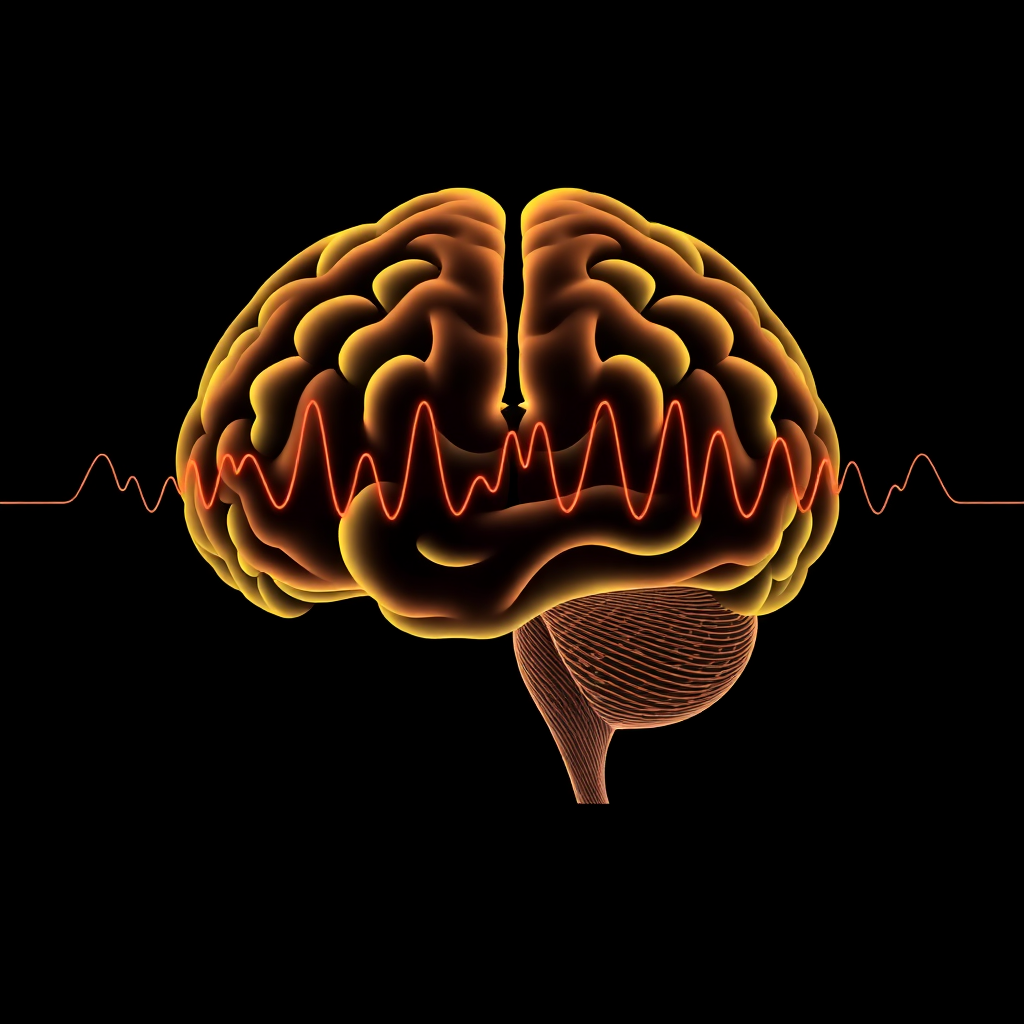
\includegraphics[width=0.8\textwidth]{images/brain_waves.png}

    \caption{Brain wave dynamics are essential for local conscious unification.}
\end{figure}

The role of electromagnetic fields in establishing and maintaining neural coherence finds substantial empirical support through recent neurobiological research \cite{Frohlich2010}. Studies have demonstrated how endogenous electric fields can guide neocortical network activity, suggesting that field effects play a crucial role in coordinating neural function. These findings provide important validation for both EM field theories and ECC's broader framework of energetic coherence.

The precise timing requirements of conscious processing raise important questions about mechanisms of neural synchronization \cite{Radman2007}. EM field theories suggest that electromagnetic fields provide a natural substrate for coordinating neural activity across different brain regions. This aligns with ECC's emphasis on how coherent energy states achieve temporal integration through physical rather than computational mechanisms.

Recent theoretical work has explored how information might be integrated in the brain's electromagnetic field \cite{McFadden2020}. While traditional approaches focus on synaptic connectivity, field theories suggest that EM fields provide an additional layer of integration that helps create unified conscious experience. This perspective complements ECC's broader framework of energetic coherence while suggesting specific mechanisms for its implementation.

The relationship between field effects and neural computation \cite{Weiss2010} reveals important questions about how physical and computational processes interact in conscious systems. Rather than treating computation and field effects as separate phenomena, EM field theories suggest they are intimately connected through the brain's electromagnetic dynamics. This aligns with ECC's view that conscious processing emerges from physical rather than purely computational mechanisms.

Experimental evidence has demonstrated how electric fields can amplify and coordinate neural activity \cite{Radman2007}. These findings suggest that field effects play a more fundamental role in neural processing than previously recognized. The ability of electromagnetic fields to influence spike timing and neural excitability provides crucial support for theories that emphasize the importance of field effects in consciousness.

The binding problem in consciousness studies \cite{Singer2001} finds potential resolution through field-based approaches. Rather than requiring computational mechanisms to bind different aspects of experience together, electromagnetic fields provide a natural substrate for integration. This aligns with ECC's emphasis on how coherent energy states achieve unity through physical rather than computational processes.

Recent developments in field theory approaches have emphasized how electromagnetic fields might contribute to both local and global aspects of conscious processing \cite{John2001}. The ability of fields to influence neural activity across multiple scales suggests they play a crucial role in creating the integrated yet differentiated character of conscious experience.

The question of how electromagnetic fields contribute to neural information processing remains an active area of investigation \cite{Barrett2011}. While some researchers emphasize the computational aspects of field effects, others focus on their role in coordinating and integrating neural activity. ECC suggests these perspectives might be unified by understanding how coherent energy states naturally support both information processing and integration through their physical dynamics.

Recent theoretical work has explored how electromagnetic fields might contribute to consciousness through their influence on neural timing and synchronization \cite{Pockett2012}. The ability of fields to coordinate activity across different neural populations suggests they play a crucial role in creating the temporal coherence characteristic of conscious experience. This aligns with ECC's emphasis on how physical mechanisms support conscious integration.

The relationship between attention and electromagnetic field effects \cite{Prinz2012} reveals important questions about conscious control mechanisms. While traditional approaches focus on synaptic mechanisms of attention, field theories suggest that electromagnetic fields might provide an additional layer of control over neural processing. This perspective complements ECC's broader framework while suggesting specific mechanisms for attentional modulation.

Empirical studies have demonstrated how electromagnetic fields shape morphogenesis and consciousness through environmental orchestration \cite{Rouleau2014}. These findings suggest that field effects play a fundamental role in both the development and ongoing function of conscious systems. This provides important support for theories that emphasize the importance of field effects in biological organization.

The integration of electromagnetic approaches with broader theories of consciousness \cite{McFadden2020} suggests productive new directions for research. By examining how field effects contribute to conscious processing while maintaining connection to other physical mechanisms, we may develop more sophisticated understanding of how consciousness emerges from biological systems.

These theoretical syntheses reveal important connections between electromagnetic field theories and other approaches to consciousness \cite{John2001}. While EM field theories provide crucial insights about specific physical mechanisms, ECC suggests these mechanisms operate within a broader framework of energetic coherence. This integration offers promising directions for future research into the physical basis of consciousness.

The future development of field-based approaches to consciousness will likely require sophisticated integration of theoretical insights with empirical investigation \cite{Singer2001}. By examining how electromagnetic fields contribute to conscious processing while maintaining connection to other physical mechanisms, we may develop increasingly sophisticated understanding of how consciousness emerges from biological systems.

In support of the EM Field view, recent research has significantly advanced our understanding of ephaptic coupling's role in neural information processing and potential contributions to consciousness. Evidence suggests that electric fields generated by neural activity can directly influence nearby neurons through non-synaptic mechanisms, creating a form of neural communication that operates alongside traditional synaptic transmission \cite{Pinotsis2023Ephaptic}. These field effects may contribute to the formation and stabilization of memory networks, suggesting a broader role for electromagnetic fields in neural information processing than previously recognized.

The concept of cytoelectric coupling has emerged as particularly significant, describing how electric fields can sculpt neural activity patterns and effectively "tune" the brain's infrastructure \cite{Pinotsis2023Cytoelectric}. Detailed modeling work has demonstrated that these ephaptic effects operate at the mesoscopic scale in human brain tissue, potentially contributing to neural synchronization and information integration \cite{Reimann2020Modeling}. Recent theoretical analysis suggests that ephaptic coupling may fundamentally contribute to brain complexity \cite{Cunha2024Ephapticity}, while studies of coincidence detector neurons in the auditory brainstem have revealed how endogenous electric fields can influence neural timing and synchronization \cite{Goldwyn2016Neuronal}. These findings align with ECC's emphasis on field effects in conscious processing, suggesting that ephaptic coupling might represent one mechanism through which the brain maintains the coherent energy states necessary for consciousness.

The role of ephaptic coupling in neural information processing suggests intriguing possibilities for how electromagnetic fields contribute to conscious experience. Beyond merely serving as a byproduct of neural activity, these fields may actively shape neural dynamics across multiple spatial scales. The ability of electric fields to modify neural timing and synchronization through ephaptic effects \cite{Goldwyn2016Neuronal} could provide a physical mechanism for the kind of rapid information integration that consciousness requires.

Research into memory network formation through ephaptic coupling \cite{Pinotsis2023Ephaptic} reveals how field effects might contribute to the stability of conscious states while allowing for dynamic reorganization. The concept of cytoelectric coupling \cite{Pinotsis2023Cytoelectric} suggests that electromagnetic fields play an active role in shaping neural architecture, potentially creating the conditions necessary for conscious processing through continuous field-mediated feedback between neurons and their environment.

Detailed modeling of mesoscopic ephaptic coupling in human brain tissue \cite{Reimann2020Modeling} has demonstrated that these effects operate at scales relevant for conscious integration. The contribution of ephaptic coupling to brain complexity \cite{Cunha2024Ephapticity} aligns with ECC's emphasis on consciousness requiring sophisticated patterns of energetic coherence. These findings suggest that ephaptic coupling might represent a crucial mechanism through which the brain achieves the field coherence necessary for conscious experience while maintaining the flexibility required for adaptive behavior.

This research indicates that electromagnetic fields in neural tissue serve not merely as epiphenomena but as active participants in neural information processing and conscious integration. The ability of ephaptic coupling to influence neural timing and synchronization without direct synaptic contact provides a potential physical basis for the kind of field-mediated integration that consciousness appears to require. These insights strengthen ECC's emphasis on field effects while suggesting specific mechanisms through which these fields might contribute to conscious experience.

\section{Basal Cognition}

Lynn Margulis' work on cellular consciousness and symbiogenesis, alongside recent research \cite{Lyon2015}, reveals that even simple cellular collectives demonstrate remarkable information processing capabilities through bioelectric signaling and membrane dynamics. Margulis' insight that consciousness has roots in bacterial awareness \cite{Margulis2001}, combined with contemporary findings \cite{Baluska2016}, suggests that the complex electromagnetic fields supporting consciousness in neural tissue represent an elaboration of primitive cellular communication mechanisms rather than a novel innovation.

The key insights from recent theoretical work show that cognitive-like processes—decision-making, memory, and pattern recognition—exist at the cellular level without requiring neurons or synapses \cite{Shapiro2007}. These capabilities depend critically on bioelectric fields and membrane potentials, the same physical phenomena that, at a more complex level, contribute to conscious processing in neural tissue. Research on bacterial consciousness \cite{vanDuijn2006} and bioelectric fields suggests consciousness emerged through the progressive refinement and integration of basic cellular awareness mechanisms rather than appearing suddenly with neural complexity.

Recent work \cite{Lane2015} complements these perspectives by emphasizing how membrane dynamics and ion gradients form the basis of all biological information processing. The ability to maintain ion gradients across membranes represents one of life's fundamental innovations, enabling both energy storage and information processing. This dual role of membranes—as both energetic and informational structures—aligns with both cellular approaches to consciousness and ECC's emphasis on the inseparability of energy dynamics and conscious processing.

Contemporary research on basal cognition \cite{Levin2019} demonstrates that cognitive capabilities emerge from fundamental cellular processes. These findings suggest consciousness evolved not merely through increasing neural complexity but through the progressive elaboration of basic cellular awareness mechanisms that were present from life's earliest stages. The convergence of these perspectives provides strong support for ECC's emphasis on energetic coherence as fundamental to consciousness.

Theoretical developments in understanding biological computation \cite{Levin2018} suggest a deeper physical basis for conscious processing. The electromagnetic fields that help sustain conscious states through neural light cones may represent a sophisticated elaboration of more basic bioelectric fields present in all cells. The complex interference patterns possible in neural tissue might have evolved from simpler patterns of membrane potential coordination in cellular collectives.

The rich alphabet that ECC posits as necessary for consciousness—implemented through transcriptomic profiles and protein configurations—may have its origins in the diverse membrane proteins and ion channels that enable basic cellular cognition \cite{Fields2020}. This suggests a continuity between basal cellular information processing and conscious experience that helps explain how consciousness could have emerged through evolution.

Recent work on biological decision-making \cite{Mitchell2016} demonstrates how even simple cellular systems achieve sophisticated information processing through molecular mechanisms. These findings support the idea that consciousness represents an elaboration of fundamental biological capabilities rather than a completely novel emergence.

The relationship between basal cognition and membrane dynamics becomes even richer when considering the role of genetic regulation \cite{Manicka2019}. DNA can be understood as providing metaprograms that shape cellular behavior across different timescales, while RNA serves as more immediate programs that fine-tune cellular responses through transcriptomic profiles. This hierarchical regulatory system fundamentally shapes both basal cognition and membrane dynamics.

The cognitive capabilities of cellular systems \cite{Lyon2015} demonstrate sophisticated information processing without requiring neural architecture. Recent work has shown how cells achieve complex computational tasks through membrane dynamics and bioelectric signaling \cite{Levin2018}. These findings suggest that consciousness builds upon fundamental cellular mechanisms rather than emerging solely from neural complexity.

Research on bacterial cognition \cite{Shapiro2007} reveals remarkable decision-making capabilities in simple organisms. These studies demonstrate how basic cellular processes support sophisticated information processing through membrane dynamics and molecular signaling. The cognitive capabilities of bacteria suggest that consciousness represents an elaboration of fundamental biological mechanisms rather than a novel emergence.

The physical basis of biological computation \cite{Pattee2001} takes on particular significance when examining basal cognition. Rather than implementing abstract computational processes, cellular systems achieve information processing through concrete physical mechanisms involving membrane dynamics and molecular interactions. This aligns with ECC's emphasis on how consciousness emerges from physical rather than purely computational processes.

Recent theoretical work \cite{Fields2020} has emphasized how scale-free principles operate across biological systems. The same fundamental mechanisms that enable cellular cognition may scale up to support more complex forms of consciousness through progressive elaboration and integration. This suggests important continuities between basic cellular processing and conscious experience.

The role of bioelectric fields in morphogenesis and cognition \cite{Levin2019} provides crucial insight into how cellular mechanisms support information processing. These fields coordinate cellular behavior across multiple scales, suggesting how simple awareness mechanisms might have evolved into more complex forms of consciousness. The ability of bioelectric fields to influence both development and cognition reveals important connections between cellular and neural processing.

Studies of minimal cognition in simple organisms \cite{vanDuijn2006} demonstrate how basic biological mechanisms support sophisticated information processing. These findings suggest that consciousness emerges from fundamental cellular capabilities rather than requiring entirely new mechanisms. The cognitive abilities of simple organisms provide important insight into how consciousness might have evolved from basic cellular processes.

The relationship between cellular and conscious information processing \cite{Margulis2001} gains new significance when examined through modern theoretical frameworks. Recent studies of basal cognition \cite{Levin2018} demonstrate how fundamental cellular mechanisms achieve sophisticated computation through physical rather than abstract processes. This suggests consciousness represents an elaboration of basic biological capabilities rather than a wholly novel phenomenon.

The computational boundary of biological systems \cite{Levin2019} reveals important questions about how information processing scales across different levels of organization. While traditional approaches often treat computation as abstract symbol manipulation, research on cellular cognition suggests that biological information processing emerges from concrete physical mechanisms. This aligns with ECC's emphasis on how consciousness arises from actual physical dynamics rather than purely computational processes.

Studies of cognitive cell biology \cite{Mitchell2016} have demonstrated how cellular decisions emerge from complex molecular interactions. Rather than implementing abstract algorithms, cells achieve sophisticated information processing through the physical dynamics of membrane potentials and molecular signaling. These findings suggest important continuities between cellular cognition and conscious processing.

Recent theoretical developments \cite{Fields2020} emphasize how biological computation operates across multiple scales through consistent principles. The same mechanisms that enable cellular decision-making may support more complex forms of consciousness through progressive elaboration and integration. This suggests consciousness represents an extension of fundamental biological capabilities rather than requiring entirely new mechanisms.

The role of molecular communication in cellular cognition \cite{Manicka2019} provides crucial insight into how biological systems achieve information processing. Rather than implementing abstract computation, cells process information through concrete physical mechanisms involving membrane dynamics and molecular interactions. This aligns with ECC's emphasis on how consciousness emerges from actual physical processes.

These theoretical syntheses suggest productive new directions for consciousness research that examine how basic cellular mechanisms support increasingly sophisticated forms of awareness \cite{Baluska2016}. By understanding how consciousness emerges from fundamental biological processes, we may develop more sophisticated theories that bridge cellular and neural approaches to mind while maintaining closer contact with physical reality.

The future investigation of consciousness may require careful examination of how basic cellular mechanisms elaborate into more complex forms of awareness \cite{Lyon2015}. This suggests new experimental approaches that examine consciousness across multiple scales of biological organization while maintaining connection to fundamental physical processes.

\section{Quantum Theories}

The Penrose-Hameroff Orchestrated Objective Reduction (Orch OR) theory \cite{Hameroff2014} represents perhaps the most developed quantum theory of consciousness, proposing that quantum computations in microtubules give rise to conscious experience. While ECC does not depend on quantum effects for its core mechanisms, certain aspects of quantum physics might influence the electromagnetic fields that help sustain conscious states.

Early work exploring quantum aspects of brain activity \cite{Beck1992} suggested potential roles for quantum mechanics in neural processing. However, ECC maintains that classical electromagnetic fields and molecular dynamics provide sufficient basis for understanding conscious processing. The complex interference patterns possible in neural tissue, combined with the rich alphabet of protein states and membrane dynamics, may not require quantum effects to explain conscious experience.

Critical analysis of quantum approaches \cite{Tegmark2000} has raised important questions about the feasibility of maintaining quantum coherence in the warm, wet environment of the brain. ECC aligns with this perspective, suggesting that consciousness emerges from classical field dynamics that operate at scales above quantum decoherence thresholds. This classical approach aligns with the thermodynamic constraints observed in biological systems.

The philosophical implications of quantum consciousness theories \cite{Stapp2009} raise fundamental questions about the relationship between mind and matter. While quantum theories often suggest consciousness requires quantum effects, ECC proposes that classical field dynamics provide sufficient basis for understanding how consciousness emerges from physical systems. This maintains closer connection to established biological mechanisms while avoiding speculative quantum requirements.

Recent theoretical developments \cite{Hagan2002} have attempted to address the decoherence challenge by proposing specific mechanisms for maintaining quantum coherence in biological systems. However, ECC suggests that even if quantum effects play some role in neural processing, consciousness itself emerges from classical patterns of energetic coherence that operate at larger scales.

Early philosophical work on quantum mechanics and consciousness \cite{Bohm1990} proposed deep connections between quantum processes and mental phenomena. While these perspectives raise important questions about the nature of consciousness, ECC suggests that understanding conscious experience requires examining classical field dynamics rather than quantum effects.

The relationship between quantum mechanics and brain function \cite{Koch2006} remains a matter of ongoing investigation. While quantum effects might influence certain aspects of neural processing, ECC proposes that consciousness emerges from classical patterns of energetic coherence that can be understood without invoking quantum mechanisms.

Although Penrose's early proposals \cite{Penrose1989, Penrose1994} suggested fundamental connections between quantum processes and consciousness, ECC suggests that classical field dynamics provide a more plausible physical basis for conscious experience. While quantum effects might operate at microscopic scales, the coherent energy patterns that support consciousness likely emerge from classical mechanisms operating at larger scales.

Detailed physical analysis \cite{Tegmark2000} has demonstrated significant challenges for quantum consciousness theories, particularly regarding decoherence timescales in biological systems. The brain operates at temperatures and scales where quantum coherence is difficult to maintain, though quantum effects might still influence field dynamics through more subtle mechanisms, including:

The mathematical frameworks developed for quantum consciousness \cite{Hagan2002} have contributed valuable insights about potential physical mechanisms of consciousness. However, ECC suggests that understanding consciousness requires examining classical field dynamics rather than quantum effects, while acknowledging that quantum properties might influence these classical fields in subtle ways.

Recent work on quantum biology \cite{Koch2006} has revealed quantum effects in certain biological processes, such as photosynthesis and magnetic sensing. While these findings demonstrate that quantum mechanisms can operate in biological systems, ECC maintains that consciousness itself likely emerges from classical patterns of energetic coherence rather than requiring quantum computation.

The relationship between quantum mechanics and brain function \cite{Stapp2009} raises important questions about causation and measurement in conscious systems. While quantum theories often invoke measurement problems to explain consciousness, ECC suggests that conscious experience emerges from classical field dynamics that can be understood without reference to quantum measurement paradoxes.

The original proposals linking quantum mechanics to consciousness \cite{Beck1992} highlighted important questions about the physical basis of mental phenomena. However, ECC suggests that understanding consciousness requires examining classical field dynamics rather than quantum effects, while maintaining the possibility that quantum properties might influence these classical patterns in subtle ways.

Recent theoretical developments \cite{Hameroff2014} have attempted to address criticisms of quantum consciousness theories by proposing specific mechanisms for maintaining quantum coherence. However, ECC suggests that even if such mechanisms exist, consciousness itself likely emerges from classical patterns of energetic coherence operating at scales above quantum decoherence thresholds.

The microtubule hypothesis central to quantum theories \cite{Hameroff2014} raises important questions about cellular organization in consciousness. While ECC acknowledges the importance of microtubules in cellular function, it suggests their role emerges through classical rather than quantum mechanisms. From a purely classical perspective, microtubules serve as crucial integrative structures that, like membranes, play essential roles in both information processing and mechanical output.

Building on foundational quantum approaches \cite{Penrose1989}, recent work has explored potential quantum effects in neural systems. However, ECC suggests that understanding consciousness requires examining classical field dynamics that operate at scales where quantum coherence is unlikely to persist. This aligns with critical analyses \cite{Tegmark2000} demonstrating the challenges of maintaining quantum states in biological systems.

The philosophical implications of quantum consciousness theories \cite{Bohm1990} extend beyond purely physical considerations. While these approaches often suggest deep connections between quantum mechanics and mind, ECC proposes that conscious experience emerges from classical patterns of energetic coherence that can be understood without invoking quantum effects.

Contemporary research on quantum biology \cite{Koch2006} has revealed quantum effects in specific biological processes. However, ECC maintains that consciousness itself likely emerges from classical mechanisms, even if quantum effects influence certain aspects of cellular function. This perspective aligns with empirical evidence about the scales at which conscious processing occurs.

The relationship between quantum mechanics and consciousness \cite{Stapp2009} remains contentious within neuroscience. While quantum theories offer intriguing possibilities, ECC suggests that understanding consciousness requires examining classical field dynamics that operate at scales where quantum effects are unlikely to play a direct role.

These theoretical syntheses suggest productive new directions for consciousness research that examine both classical and quantum mechanisms \cite{Hagan2002}. By understanding how different physical processes contribute to conscious experience across multiple scales, we may develop more sophisticated theories that bridge quantum and classical approaches while maintaining closer contact with biological reality.

The future investigation of consciousness will likely require careful examination of how different physical mechanisms interact across scales \cite{Beck1992}. This suggests new experimental approaches that examine consciousness at multiple levels of organization while maintaining connection to fundamental physical processes.

\section{Embodied Consciousness}

The relationship between consciousness and embodiment has been extensively explored in foundational work \cite{Varela1991, MerleauPonty1962} that emphasizes how conscious experience emerges from the dynamic coupling between organism and environment. Where traditional cognitive science often treats the body as merely an input-output system for an abstract mind, both phenomenological approaches and ECC emphasize how consciousness emerges from the concrete dynamics of biological organization.

Recent theoretical developments \cite{Thompson2007} have emphasized how consciousness cannot be understood in isolation from the physical body and its environmental interactions. This perspective resonates with ECC's framework in several important ways, particularly regarding how patterns of energetic coherence emerge from and support embodied activity. The framework suggests that consciousness requires specific forms of physical organization that cannot be reduced to computational representation.

Early phenomenological insights \cite{MerleauPonty1962} about the primacy of embodied perception anticipated many contemporary developments in consciousness studies. The concept of the "body schema" - our implicit understanding of our body's capabilities and position - can be understood through ECC as emerging from patterns of energetic coherence that span brain and body rather than abstract representation.

Contemporary work on embodied cognition \cite{Clark1997} has demonstrated how consciousness emerges from the dynamic interaction between organism and environment. While some approaches attempt to reduce embodiment to computational models, ECC reveals how consciousness emerges from actual patterns of energetic coherence that cannot be adequately captured through computational representation.

The philosophical foundations of embodied consciousness \cite{Lakoff1999} emphasize how mental processes are fundamentally shaped by physical embodiment. ECC strengthens this position by demonstrating how consciousness emerges from specific patterns of energetic coherence maintained through biological systems, rather than from abstract computation alone.

Research on skilled action and embodied knowledge \cite{Ingold2000} reveals how consciousness emerges from practical engagement with the environment. Rather than treating bodily processes as inputs to be modeled, ECC shows how consciousness is inherently embodied through its physical emergence from coherent energy dynamics.

Anthropological perspectives on embodiment \cite{Csordas1994} have emphasized how conscious experience is shaped by cultural and physical practices. ECC provides a physical framework for understanding how these embodied practices influence consciousness through their effects on patterns of energetic coherence.

The anticomputationalist stance developed in seminal work \cite{Dreyfus1992} finds support in ECC's demonstration that consciousness requires specific forms of physical organization that cannot be reduced to computation. This perspective challenges attempts to reduce embodied cognition to computational representations of bodily states, suggesting instead that consciousness emerges from actual physical dynamics.

Recent research on the relationship between body and mind \cite{Gallagher2005} has revealed how consciousness emerges from embodied activity rather than abstract mental processes. ECC extends this insight by showing how patterns of energetic coherence necessarily span both brain and body, creating an integrated field of conscious experience that cannot be reduced to purely neural computation.

The phenomenology of bodily experience \cite{Leder1990} takes on new significance when examined through ECC's framework. Rather than treating bodily awareness as a form of internal representation, ECC suggests that conscious bodily experience emerges directly from patterns of energetic coherence that naturally span neural and bodily tissues.

Contemporary work on perception and action \cite{Noe2004} emphasizes how conscious experience emerges from active engagement with the environment. ECC provides a physical basis for understanding this relationship, showing how patterns of energetic coherence naturally support both perception and action through their embodied dynamics.

Theoretical developments in embodied cognition \cite{Thompson2007} have demonstrated how consciousness requires ongoing interaction between organism and environment. Rather than treating this interaction as computational input-output, ECC reveals how conscious experience emerges from continuous patterns of energetic coherence that span brain, body, and environment.

Anthropological studies of skilled practice \cite{Marchand2010} show how consciousness emerges from embodied engagement with the world. ECC provides a physical framework for understanding how these practices shape consciousness through their effects on patterns of energetic coherence rather than through abstract representation.

Studies of sensory experience \cite{Howes2003} reveal how consciousness emerges from multiple forms of bodily engagement with the environment. ECC suggests that this multisensory integration occurs through patterns of energetic coherence that naturally span different sensory modalities rather than requiring computational binding mechanisms.

The relationship between embodiment and conscious experience \cite{Jackson1989} gains new significance when examined through ECC's framework. Rather than treating embodiment as an implementation detail, ECC reveals how consciousness necessarily emerges from specific patterns of energetic coherence that span brain and body, making embodiment essential rather than incidental to conscious experience.

Recent work on the philosophical implications of embodiment \cite{Lakoff1999} aligns with ECC's demonstration that consciousness cannot be reduced to abstract computation. The framework shows how conscious experience requires actual physical dynamics that emerge from biological organization rather than computational representation of bodily states.

The ecological approach to perception \cite{Gibson1979} finds natural extension through ECC's emphasis on how consciousness emerges from organism-environment interaction. Rather than treating perception as internal representation, ECC shows how perceptual experience emerges from patterns of energetic coherence that naturally span perceiver and environment.

Studies of skilled bodily practice \cite{Ingold2000} reveal how consciousness emerges from embodied engagement with the world. ECC provides a physical framework for understanding how these practices shape consciousness through their effects on patterns of energetic coherence rather than through abstract mental representations.

Contemporary research on embodied cognition \cite{Clark1997} demonstrates how consciousness requires ongoing interaction between organism and environment. ECC extends this insight by showing how patterns of energetic coherence necessarily span brain, body, and environment, creating an integrated field of conscious experience.

Phenomenological investigations \cite{MerleauPonty1962} have long emphasized the primacy of embodied experience. ECC provides physical mechanisms that explain how consciousness emerges from embodied dynamics, supporting phenomenological insights while grounding them in concrete physical processes.

These theoretical syntheses suggest new directions for investigating how consciousness emerges from embodied activity \cite{Varela1991}. By examining how patterns of energetic coherence span brain, body, and environment, we may develop more sophisticated understanding of consciousness while maintaining closer contact with physical reality.

\newpage
\section{References}
\printbibliography[title={},heading=subbibliography]
%\printbibliography[title={Comparative Analysis: Embodied Consciousness}]
\end{refsection}

\section*{\phantom{Part X Future Directions}}
\h{Future Directions}

\begin{refsection}[references//0001_8_future_dirs.bib]

The future development of Energetically Coherent Computation requires systematic investigation across multiple domains, from molecular mechanisms to clinical applications. This section examines key research directions for validating and extending ECC's framework while maintaining rigorous scientific standards.

Several crucial areas emerge for future investigation. First, testing ECC demands sophisticated experimental approaches capable of measuring and manipulating patterns of energetic coherence while assessing their relationship to conscious experience. These methods must span multiple scales of organization, from cellular dynamics to whole-brain states, while maintaining careful control over experimental variables.

Animal models provide another essential avenue for investigation, offering natural experiments in how different neural architectures support conscious processing. The comparative study of consciousness across species helps identify which aspects of neural organization prove truly necessary for conscious experience versus those that merely represent one possible implementation.

Brain organoids and wetware computing systems present unique opportunities for studying consciousness-supporting mechanisms in controllable yet biologically authentic environments. These simplified but realistic neural tissues enable systematic investigation of how patterns of energetic coherence emerge and maintain stability, while avoiding some of the complexity and ethical challenges of working with intact brains.

Novel predictions generated by ECC provide concrete directions for empirical validation. These predictions span biological, thermodynamic, clinical, computational, and developmental domains, offering multiple avenues for testing the theory's fundamental claims. The systematic investigation of these predictions requires careful integration of multiple experimental approaches while maintaining methodological rigor.

The future directions outlined in this section suggest a comprehensive research program for advancing our understanding of consciousness through the lens of energetic coherence. Success in these endeavors requires careful balance between innovative methodological approaches and established scientific principles, while maintaining clear connection to empirically measurable phenomena.

\section{Testing ECC}

Testing ECC requires a multi-scale approach that examines both the physical foundations of energetic coherence and its relationship to conscious experience. The empirical validation must span multiple domains while maintaining methodological rigor.

High-temporal resolution neuroimaging combined with thermodynamic measurements offers one crucial direction for testing ECC's core predictions. Temperature mapping during neural recording can track patterns of energy flow and coherence across brain regions \cite{Watts2018}. By examining how thermal gradients correlate with conscious processing, researchers can evaluate whether energetic coherence follows the proposed constraints of neural light cones.

The analysis of scale-free brain activity provides another essential avenue for investigating ECC's framework. Recent work has demonstrated how neural dynamics maintain coherent patterns across multiple temporal and spatial scales \cite{He2014}. This scale-free organization aligns with ECC's emphasis on coordinated energy flows spanning different levels of neural architecture.

Transcriptomic analysis represents a particularly promising direction for testing ECC's predictions about regional specialization. Single-cell RNA sequencing enables detailed examination of how gene expression patterns shape local "alphabets" for conscious encoding \cite{Gallegos2020}. This molecular profiling can reveal whether regions supporting conscious processing demonstrate predicted patterns of transcriptomic diversity and energy management.

Clinical applications offer natural experiments for testing ECC's framework. Analysis of resting state networks in disorders of consciousness could reveal how different patterns of energetic disruption correlate with specific impairments \cite{Fox2010}. The relationship between network connectivity and conscious awareness may illuminate fundamental principles about how coherent energy states support conscious experience.

The investigation of brain metabolism through advanced imaging techniques enables direct testing of ECC's energetic predictions \cite{Magistretti2018}. By examining how different brain regions manage energy distribution during conscious tasks, researchers can evaluate whether conscious processing demonstrates the predicted patterns of metabolic efficiency and coherence.

Brain network analysis provides crucial tools for examining how patterns of energetic coherence emerge and maintain stability \cite{DePasquale2020}. The dynamic reorganization of neural networks during development and pathological conditions offers important opportunities for testing ECC's predictions about the relationship between network architecture and conscious processing.

These empirical approaches must be integrated within a broader theoretical framework that bridges physical mechanisms and conscious experience \cite{Northoff2020}. The systematic investigation of ECC's predictions requires careful attention to both methodological rigor and theoretical grounding to establish clear relationships between energetic coherence and conscious states.

Development of new analytical tools will prove essential for quantifying and characterizing patterns of energetic coherence. Advanced signal processing techniques combined with machine learning approaches can help identify organizational principles that might not be apparent through traditional analysis methods \cite{Buzsaki2019}. These tools must maintain careful balance between sophisticated measurement approaches and scientific validity.

The empirical validation of ECC's predictions requires sophisticated methodological frameworks that track energetic coherence across different scales of biological organization. Brain networks demonstrate remarkable plasticity during both normal development and pathological conditions \cite{Vertes2015}, providing crucial opportunities to examine how patterns of energetic coherence emerge and stabilize.

The measurement of cellular energy metabolism offers particularly valuable insights for testing ECC's framework. Advanced protocols for quantifying energy dynamics in living neural systems can reveal how different cell populations contribute to coherent energy states \cite{Zhang2019}. These measurements must track both local metabolic processes and broader patterns of energy distribution across neural tissues.

Consciousness research must bridge theoretical frameworks with empirical investigation \cite{Tononi2015}. ECC's predictions about the relationship between energetic coherence and conscious experience require careful validation through multiple complementary approaches. The integration of phenomenological reports with objective measurements presents significant methodological challenges that demand sophisticated experimental designs.

The thermodynamic properties of neural systems take on particular significance when examining consciousness through ECC's framework \cite{Sherrington2018}. Careful analysis of how brain regions manage energy flows during conscious processing can reveal whether the predicted patterns of thermodynamic efficiency emerge. This requires precise measurement of both energy consumption and information processing capabilities across different neural populations.

The temporal dynamics of conscious processing provide another crucial domain for testing ECC's predictions. Recent work has demonstrated how neural oscillations support temporal predictions and sensorimotor integration \cite{Palva2018}. The relationship between these rhythmic patterns and energetic coherence must be carefully examined to validate ECC's claims about temporal integration in conscious processing.

The neural basis of consciousness remains a central challenge in neuroscience \cite{Kucyi2017}. ECC's framework suggests specific mechanisms through which conscious experience emerges from patterns of energetic coherence. Testing these predictions requires careful integration of multiple measurement techniques while maintaining methodological rigor.

Clinical research provides unique opportunities for examining how disruptions to energetic coherence affect conscious experience. The systematic investigation of consciousness disorders can reveal whether specific patterns of coherence disruption correlate with particular impairments in conscious awareness. Longitudinal studies tracking recovery from brain injury might illuminate how consciousness re-emerges as coherent energy patterns are restored.

The development of new analytical tools for quantifying coherence represents another crucial aspect of experimental investigation. Advanced signal processing techniques for measuring phase relationships across frequencies, combined with information theoretical measures of local-to-global coherence, enable rigorous assessment of ECC's mathematical predictions. Machine learning approaches can help identify patterns in multi-scale energy dynamics that might not be apparent through traditional analysis methods.

The empirical investigation of ECC's predictions requires careful attention to how energetic coherence spans multiple scales of neural organization. The thermodynamic properties of neural information processing provide crucial constraints on how conscious systems maintain coherent states \cite{Sherrington2018}. Advanced imaging techniques must track both local energy dynamics and broader patterns of coherence across neural tissues.

Real-time metabolic mapping offers essential data about energy dynamics in conscious systems. Current protocols for measuring cellular energy metabolism can reveal how different neural populations contribute to coherent states \cite{Zhang2019}. These measurements must integrate analysis of both specific cellular processes and broader patterns of energy distribution across brain regions. 

Brain network analysis provides another vital avenue for testing ECC's predictions about conscious processing. Recent work has demonstrated how neural networks maintain complex patterns of coordination across multiple temporal scales \cite{Palva2018}. The relationship between these network dynamics and conscious experience must be carefully examined to validate ECC's claims about how coherent energy states support consciousness.

Clinical monitoring presents unique opportunities for testing ECC's framework in human subjects. The analysis of resting state networks in consciousness disorders could reveal how different patterns of energetic disruption correlate with specific impairments \cite{Fox2010}. Studies tracking coherence patterns during emergence from anesthesia or monitoring energy dynamics in disorders of consciousness may validate the theory's predictions about conscious state transitions.

The development of new analytical tools for quantifying coherence remains crucial. Brain network analysis techniques can reveal how patterns of energetic organization emerge and stabilize \cite{DePasquale2020}. Machine learning approaches may help identify organizational principles that are not apparent through traditional analysis methods \cite{Buzsaki2019}.

The neural basis of consciousness requires investigation through multiple complementary approaches \cite{Kucyi2017}. ECC's framework suggests specific mechanisms through which conscious experience emerges from patterns of energetic coherence. Testing these predictions requires careful integration of phenomenological reports with objective measurements while maintaining methodological rigor.

The success of these experimental approaches depends fundamentally on developing new technologies and methods capable of capturing the complex, dynamic nature of consciousness as proposed by ECC. This may require significant advances in neuroimaging, biosensors, and data analysis techniques. Future development of experimental protocols must maintain careful balance between sophisticated measurement approaches and rigorous scientific methodology.

\section{Experimental Approaches}

The empirical validation of ECC requires sophisticated experimental paradigms that can measure and manipulate energetic coherence while assessing its relationship to conscious experience. These approaches must span multiple scales of neural organization while maintaining methodological rigor and reproducibility.

Multi-modal neural recording represents a crucial foundation for testing ECC's predictions. Network neuroscience approaches combining EEG, MEG, and high-density microelectrode arrays enable tracking of coherent energy patterns across different spatial and temporal scales \cite{Bassett2017}. The integration of local field potential measurements with single-unit recordings provides crucial insight into how local coherence contributes to global conscious states.

Advanced metabolic mapping proves essential for understanding energy dynamics in conscious systems. Recent work has revealed precise energy budgets for neural computation across different brain regions \cite{Howarth2012}. Real-time measurements of glucose consumption and oxygen utilization, combined with monitoring of ATP dynamics, can reveal how conscious processing relates to energy management in neural tissues.

The development of new analytical tools for quantifying coherence represents another crucial aspect of experimental investigation. EEG microstates analysis provides valuable methods for studying the temporal dynamics of whole-brain neuronal networks \cite{Michel2018}. These techniques enable rigorous assessment of ECC's mathematical predictions about how local coherence patterns integrate into global conscious states.

Clinical monitoring offers unique opportunities for testing ECC's frameworks in human subjects. Studies of global resting-state fMRI activity have revealed important principles about how brain networks maintain coherent activity patterns \cite{Scholvinck2013}. These natural experiments in clinical settings offer crucial insight into how consciousness relates to patterns of energetic coherence in human brains.

The investigation of default mode network activity provides another vital avenue for understanding conscious processing \cite{Raichle2015}. By examining how different brain regions achieve and maintain coherent baseline states, researchers can evaluate ECC's predictions about the relationship between energy dynamics and conscious experience.

Advanced nanoelectronic devices for brain mapping enable unprecedented precision in measuring neural activity patterns \cite{Kuzum2014}. These tools provide essential capabilities for tracking how coherent energy states propagate through neural tissues at multiple scales. The development of such sophisticated recording technologies proves crucial for validating ECC's predictions about consciousness-supporting mechanisms.

The success of these experimental approaches depends fundamentally on developing new technologies and methods capable of capturing the complex, dynamic nature of consciousness as proposed by ECC. This may require significant advances in neuroimaging, biosensors, and data analysis techniques. Future development of experimental protocols must maintain careful balance between sophisticated measurement approaches and rigorous scientific methodology.

The relationship between synaptic plasticity and conscious processing provides another crucial domain for investigation. Recent work has revealed complex interactions between Hebbian plasticity and homeostatic mechanisms in neural circuits \cite{Turrigiano2017}. Understanding how these processes contribute to maintaining coherent energy states may illuminate fundamental principles about conscious processing.

These experimental considerations naturally lead us to examine how brain organoids might serve as simplified but biologically realistic systems for testing ECC's principles. The controlled nature of organoid systems, combined with their biological authenticity, offers unique opportunities for investigating how patterns of energetic coherence emerge and maintain conscious-like processing.

The experimental investigation of energetic coherence in living neural systems demands innovative technical solutions. The careful study of memory circuits through both theoretical models and empirical approaches provides crucial insights into how neural systems maintain coherent states \cite{Lisman2018}. These investigations must track both local circuit dynamics and broader patterns of network organization.

Astrocytic regulation of neural activity represents another essential domain for experimental investigation. Recent work has revealed sophisticated mechanisms through which astrocytes modulate cortical states \cite{Poskanzer2016}. Understanding how these glial cells contribute to maintaining coherent energy patterns proves crucial for validating ECC's predictions about consciousness-supporting mechanisms.

The study of calcium-independent signaling pathways offers particular insight into neural excitability regulation. Research has demonstrated how astrocytic lipid release can modulate neuronal activity through mechanisms distinct from traditional calcium signaling \cite{Chow2020}. These findings suggest multiple parallel pathways through which neural systems might maintain coherent energy states.

Energy budgets in neural computation take on special significance when examining consciousness through ECC's framework. Detailed analysis of energy consumption across different brain regions reveals remarkable efficiency in neural information processing \cite{Bezaires2013}. These energetic constraints must be carefully considered when evaluating how conscious systems maintain coherent states.

The relationship between sleep-wake cycles and brain energetics provides another crucial avenue for investigation. Recent work has illuminated how neural energy utilization varies across different behavioral states \cite{DiNuzzo2017}. Understanding these state-dependent changes in energy dynamics may reveal fundamental principles about how consciousness emerges from coherent energy patterns.

Optogenetic approaches enable precise manipulation of neural circuits during experimental investigation \cite{Yizhar2011}. These tools allow researchers to perturb specific aspects of neural processing while monitoring effects on coherent energy states. Such targeted interventions prove essential for establishing causal relationships between neural activity patterns and conscious processing.

The experimental investigation of consciousness demands careful integration of multiple measurement approaches. Theoretical frameworks for conscious processing must be grounded in empirical observations that span multiple scales of neural organization \cite{Dehaene2011}. This integration of theory and experiment remains crucial for advancing our understanding of how consciousness emerges from coherent energy dynamics.

The integration of multiple experimental approaches requires sophisticated analytical frameworks. Brain network analysis has revealed fundamental principles about how neural systems maintain coordinated activity across different scales \cite{Bassett2017}. These network approaches must be combined with detailed energy measurements to understand how conscious processing emerges from coherent states.

The relationship between neural energy consumption and information processing provides crucial insight into consciousness-supporting mechanisms. Careful analysis of energy budgets across different brain regions has revealed remarkable efficiency in neural computation \cite{Howarth2012}. Understanding these energetic constraints proves essential for validating ECC's predictions about how conscious systems maintain coherent states.

The investigation of resting-state networks offers particular value for understanding baseline consciousness. Global patterns of neural activity during rest reveal important principles about how brain networks maintain coherent states \cite{Scholvinck2013}. These intrinsic activity patterns may reflect fundamental mechanisms through which consciousness emerges from energetic coherence.

Experimental protocols must carefully balance the need for precise measurement with maintenance of natural neural dynamics. Advanced nanoelectronic devices enable unprecedented resolution in neural recording \cite{Kuzum2014}, while optogenetic techniques allow targeted manipulation of specific circuit elements \cite{Yizhar2011}. The integration of these approaches provides powerful tools for investigating how conscious processing emerges from coherent energy states.

The role of sleep in consciousness presents unique opportunities for experimental investigation. Recent work has revealed sophisticated relationships between brain energetics and sleep-wake cycles \cite{DiNuzzo2017}. Understanding how conscious states transform during sleep while maintaining the capacity for rapid awakening may illuminate fundamental principles about consciousness-supporting mechanisms.

These experimental considerations suggest multiple complementary approaches for testing ECC's predictions. By combining detailed analysis of neural energy dynamics with careful assessment of conscious states, researchers can evaluate whether patterns of energetic coherence indeed correlate with and support conscious processing as the theory predicts.

The success of this experimental program depends critically on maintaining rigorous standards while embracing innovative methodological approaches. Through careful integration of multiple measurement techniques and sophisticated analytical tools, researchers can build a comprehensive understanding of how consciousness emerges from coherent energy dynamics in biological systems.

\section{Animal Models}

The use of animal models provides crucial opportunities for testing ECC's predictions about the relationship between energetic coherence and conscious experience. Different species, with their varied neural architectures and behavioral repertoires, offer unique windows into how patterns of energetic organization support different forms of conscious processing \cite{Boly2013}.

Avian models present particularly illuminating cases for investigating ECC's framework. Despite lacking a layered neocortex, birds demonstrate sophisticated cognitive capabilities that challenge traditional assumptions about consciousness \cite{Gunturkun2016}. Their distinct neural architecture, organized through nuclear clusters rather than cortical layers, provides valuable insight into how different physical implementations can support conscious processing \cite{Clayton2015}.

The evolution of brain structure across species reveals important principles about consciousness-supporting architecture. Mosaic evolution of brain regions suggests that different aspects of conscious processing may have evolved independently in various lineages \cite{Barton2000}. This evolutionary perspective helps validate ECC's predictions about the physical requirements for consciousness while revealing multiple possible implementations.

Cephalopods offer another valuable model system due to their distributed neural architecture and sophisticated cognitive capabilities. Studies have demonstrated remarkable problem-solving abilities and potentially conscious-like behaviors in octopuses \cite{Mather2008}, despite their radically different neural organization from vertebrates. Their capacity for complex learning and memory, supported by unique neural architectures, provides crucial tests of ECC's predictions about consciousness-supporting mechanisms \cite{Teyke1989}.

Social insects present intriguing possibilities for studying emergent consciousness through collective dynamics. The sophisticated cognitive architecture of honeybee minds demonstrates how relatively simple neural systems can achieve complex information processing \cite{Menzel2001}. Their navigation capabilities and social behaviors suggest consciousness-like properties may emerge from specific patterns of neural organization even in miniaturized brains \cite{Webb2016}.

The evolutionary trajectory of centralized nervous systems provides essential context for understanding consciousness \cite{Northcutt2012}. Different organizational principles have emerged across various lineages, offering natural experiments in how conscious processing might be implemented through distinct neural architectures. This comparative approach helps identify which aspects of neural organization prove crucial for supporting conscious experience.

The comparative study of neural architectures across species illuminates fundamental principles about consciousness-supporting mechanisms. The evolution of the hippocampus in reptiles and birds demonstrates how different vertebrate lineages have developed distinct solutions for spatial cognition and memory processing \cite{Striedter2016}. These variations in neural organization help identify which aspects of brain architecture are essential for conscious processing versus those that merely represent one possible implementation.

Cross-species investigation of affective experiences provides crucial insight into the biological foundations of consciousness. Research has revealed remarkable conservation of basic emotional systems across mammals, suggesting fundamental mechanisms for conscious processing may be preserved across diverse species \cite{Panksepp2011}. This emotional conservation helps validate ECC's predictions about necessary physical conditions for supporting conscious experiences.

The relationship between brain size, structural complexity, and cognitive capabilities reveals important principles about conscious processing \cite{Roth2005}. Rather than simple scaling relationships, species differences in conscious sophistication appear to emerge from specific patterns of neural organization and connectivity. This suggests consciousness requires particular architectural features beyond mere computational capacity.

The pallium's evolution in birds and reptiles demonstrates how different vertebrate groups have achieved complex cognitive capabilities through distinct neural organizations \cite{Jarvis2009}. Despite lacking mammalian cortical organization, these species exhibit impressive behavioral flexibility and potential consciousness-like properties. Such evolutionary variations provide natural experiments for testing which aspects of neural architecture prove necessary for conscious processing.

Social signal processing across species reveals sophisticated mechanisms for integrating sensory information with behavioral responses. Research on anuran social behavior demonstrates how relatively simple nervous systems can support complex, context-dependent processing \cite{Wilczynski2010}. These findings help identify minimal requirements for consciousness-supporting neural architectures while suggesting multiple possible implementations.

The careful integration of findings across different animal models reveals fundamental principles about how consciousness emerges from neural organization. Brain structure evolution demonstrates remarkable flexibility in implementing consciousness-supporting architectures \cite{Northcutt2012}. The diversity of solutions across species suggests that consciousness requires specific organizational principles rather than particular neural architectures.

The cognitive capabilities of birds, despite their non-layered neural organization, provide especially compelling evidence for ECC's framework \cite{Clayton2015}. Their ability to achieve sophisticated conscious-like processing through nuclear rather than laminar organization demonstrates how different physical implementations can support similar functional outcomes. This architectural diversity helps identify which aspects of neural organization prove truly essential for consciousness.

The study of cephalopod cognition offers unique insights into consciousness-supporting mechanisms \cite{Mather2008}. Their remarkable behavioral flexibility, achieved through a radically different neural architecture from vertebrates, suggests consciousness can emerge from various physical implementations provided they maintain appropriate patterns of energetic coherence. This convergent evolution of consciousness-like properties helps validate ECC's fundamental predictions.

Mini-brain architectures in social insects demonstrate how relatively simple neural systems can achieve sophisticated information processing \cite{Menzel2001}. While individual insects may possess limited conscious capabilities, their collective behaviors suggest emergent properties that align with ECC's predictions about how consciousness arises from specific patterns of neural organization.

These comparative studies must be integrated within a broader theoretical framework that considers both evolutionary constraints and physical requirements for consciousness \cite{Roth2005}. The systematic investigation of consciousness across species requires careful attention to both biological variation and fundamental principles of neural organization. This comparative approach helps bridge the gap between physical mechanisms and conscious experience while maintaining scientific rigor.

These findings naturally lead us to consider how brain organoids might serve as simplified but biologically authentic systems for testing ECC's principles. The controlled nature of organoid systems, combined with their biological authenticity, offers unique opportunities for investigating how patterns of energetic coherence emerge and maintain conscious-like processing.

\section{Brain Organoids and Wetware Computing}

The integration of brain organoids with wetware computing systems presents a powerful paradigm for investigating ECC's principles in controllable yet biologically authentic environments. Brain organoids provide a unique experimental platform through their development of sophisticated cellular architectures that mirror aspects of cortical organization \cite{Lancaster2013}. These three-dimensional neural tissues enable investigation of how coherent energy patterns emerge and evolve within developing networks.

Recent advances in organoid development have demonstrated remarkable capacity for modeling human brain development and organization \cite{Quadrato2017}. These systems can be engineered with specific transcriptomic profiles and cellular compositions optimized for studying coherence dynamics. The incorporation of reporter systems for real-time energy state monitoring enables continuous tracking of how coherent patterns emerge and stabilize within developing neural networks.

The rise of three-dimensional human brain cultures offers unprecedented opportunities for studying consciousness-supporting mechanisms \cite{Pasca2018}. By combining organoid systems with wetware computing elements, researchers can create hybrid platforms that enable precise control over network architecture while maintaining biological authenticity. These approaches provide crucial windows into how consciousness-supporting mechanisms emerge from biological organization.

The marriage of biological and computational elements in wetware systems draws on fundamental principles of molecular coordination in living systems \cite{MacLennan2009}. These hybrid approaches demonstrate how information processing can emerge directly from physical dynamics rather than requiring implementation through traditional computational architectures. The success of biological computation in systems like Physarum demonstrates sophisticated information processing capabilities emerging from natural physical dynamics \cite{Adamatzky2016}.

The efficiency scaling in biological versus programmable systems reveals important principles about consciousness-supporting architectures \cite{Conrad1995}. Unlike traditional computational approaches that rely on discrete state transitions, biological systems achieve sophisticated information processing through continuous physical dynamics. This distinction proves crucial for understanding how conscious processing emerges from coherent energy states.

The bioelectric code provides another essential framework for understanding how biological systems achieve sophisticated information processing \cite{Levin2018}. Through careful regulation of bioelectric signaling, cellular networks can maintain coherent states that enable complex computation. These insights prove particularly valuable for developing hybrid systems capable of supporting consciousness-like processing.

\begin{figure}[h]
    \centering
    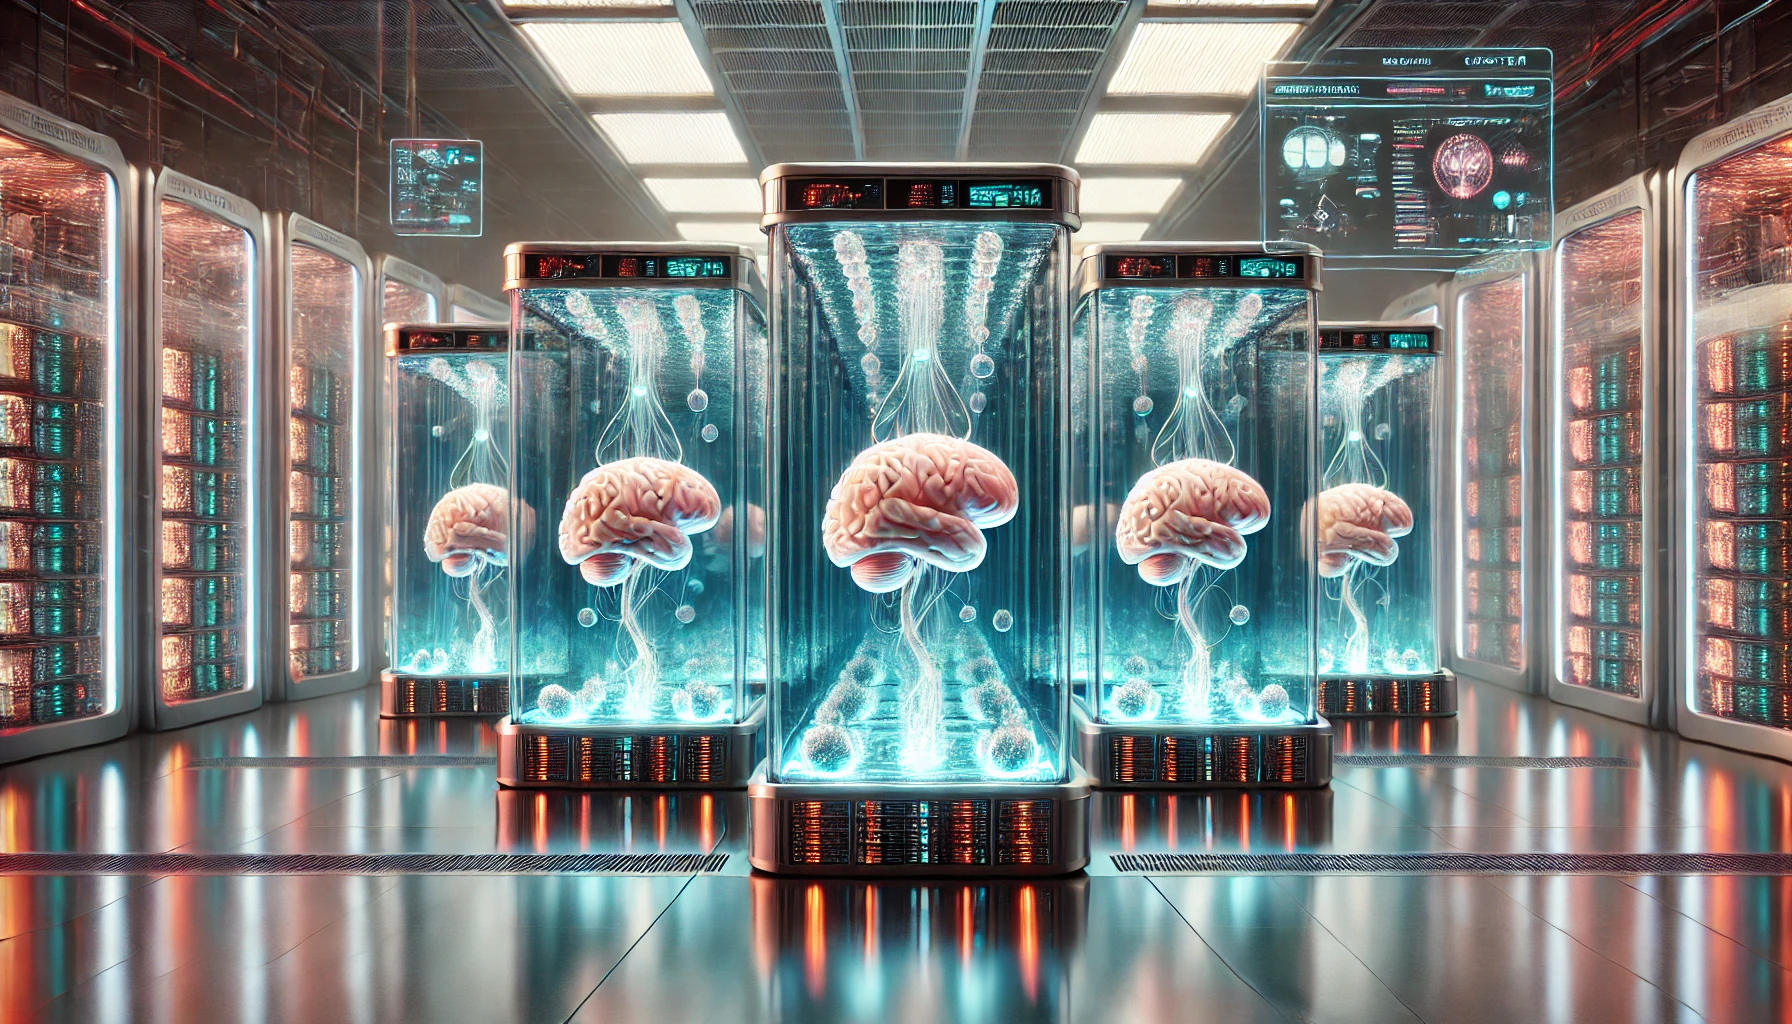
\includegraphics[width=0.8\textwidth]{organoids.png}

    \caption{A dystopic portrayal of a brain organoid data center.}
\end{figure}

The integration of biological and computational principles requires careful attention to how physical systems achieve information processing. Studies of bioelectric signaling reveal sophisticated mechanisms for controlling growth and form in biological tissues \cite{Levin2018}. These bioelectric codes demonstrate how living systems implement computation through direct physical processes rather than abstract symbol manipulation.

Advanced simulation tools enable systematic investigation of physiological signaling in biological tissues \cite{Pietak2017}. These platforms help researchers understand how coherent patterns emerge from complex cellular interactions, providing crucial insights into consciousness-supporting mechanisms. The ability to model and manipulate bioelectric fields offers new approaches for studying how conscious-like processing might emerge in engineered biological systems.

Recent developments in neuromorphic computing have demonstrated remarkable capabilities in artificial neural systems \cite{Merolla2014}. However, these digital implementations fundamentally differ from biological computation in their physical implementation. Understanding these differences helps clarify why consciousness may require specific forms of biological organization rather than merely sophisticated information processing.

The integration of living neural networks with artificial systems presents unique opportunities for investigating consciousness-supporting mechanisms \cite{DeMarse2005}. These hybrid approaches enable systematic examination of how biological neural networks achieve and maintain coherent states while processing information. The ability to interface living neurons with artificial systems provides valuable tools for testing ECC's predictions about consciousness-supporting architectures.

Ethical considerations become increasingly relevant as brain organoids achieve greater sophistication. Recent work has raised important questions about consciousness assessment in cerebral organoids \cite{Lavazza2018}. These ethical challenges require careful consideration as researchers develop more complex biological systems capable of supporting consciousness-like processing.

The experimental use of human brain tissue demands rigorous ethical frameworks \cite{Farahany2018}. As organoid systems become more sophisticated, researchers must carefully consider the potential for conscious-like properties to emerge in these tissues. This ethical dimension becomes particularly significant when developing systems specifically designed to test theories of consciousness.

\begin{figure}[h]
    \centering
    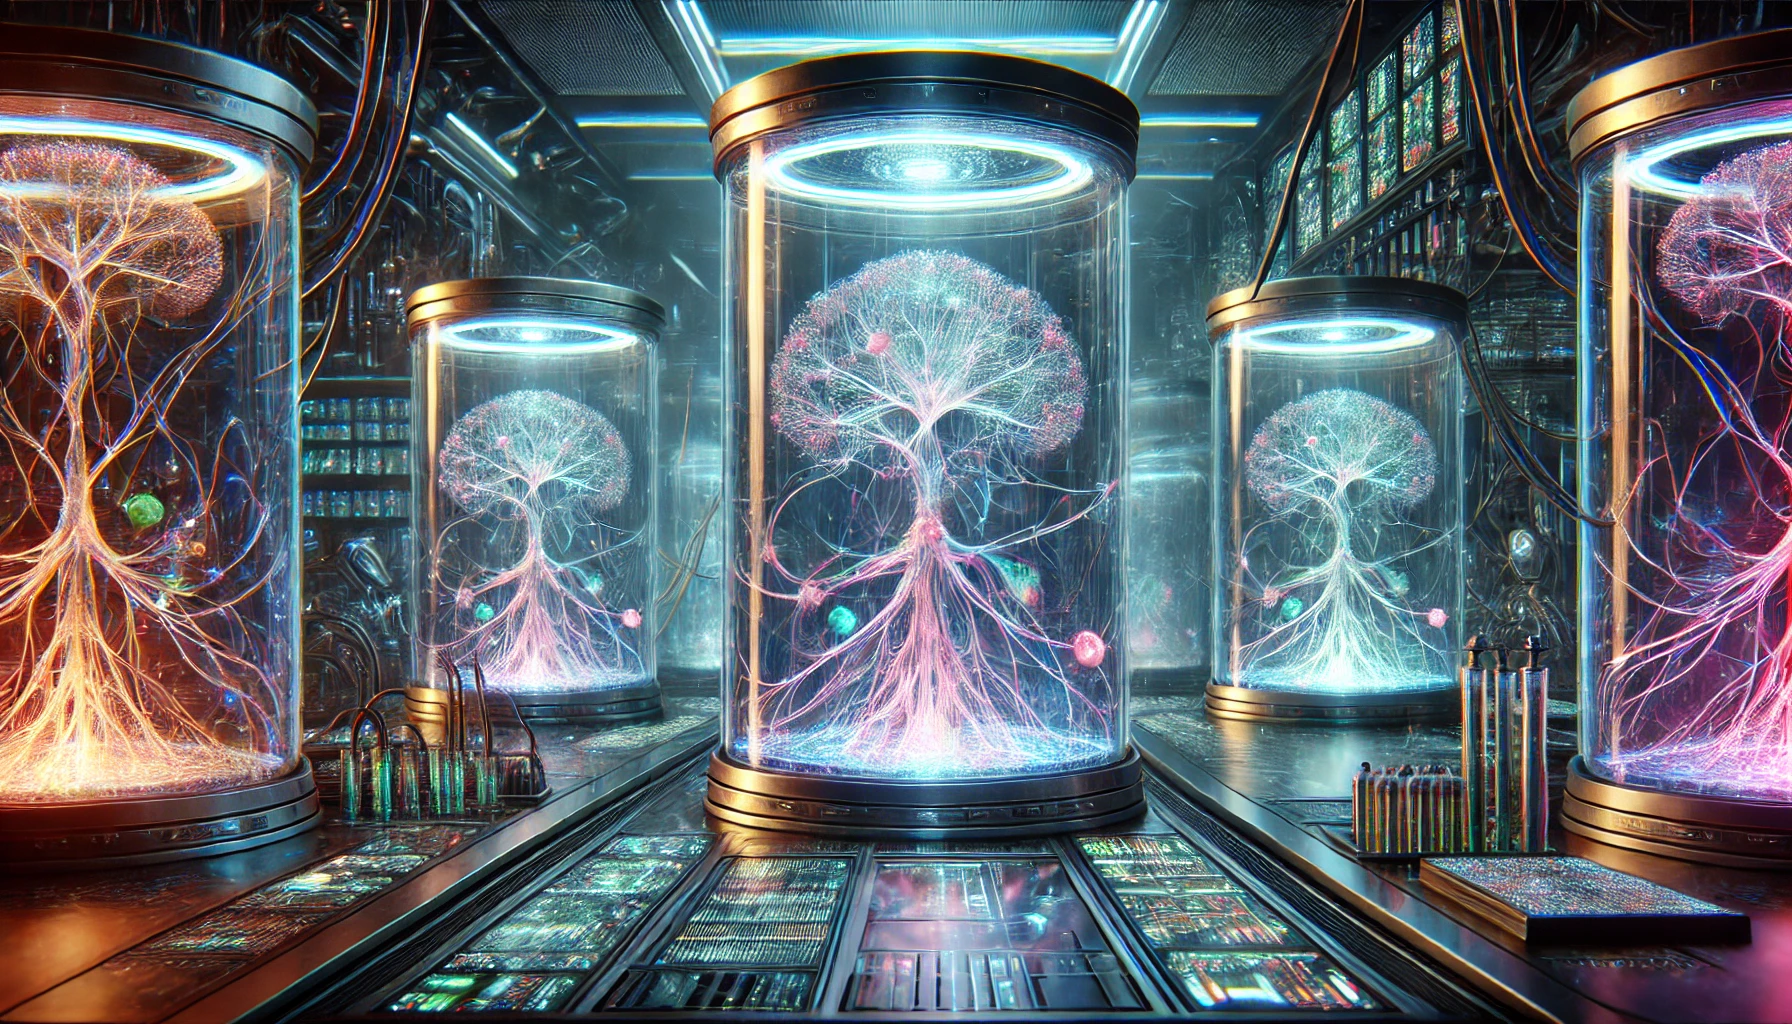
\includegraphics[width=0.8\textwidth]{wetware.png}

    \caption{Wetware computing}
\end{figure}

The integrated systems approach to biological networks reveals fundamental principles about how consciousness-supporting architectures emerge from neural organization \cite{Zhang2016}. By examining how different cellular elements interact to create coherent states, researchers can better understand the physical requirements for conscious processing. This systems-level perspective proves essential for bridging between molecular mechanisms and conscious experience.

Recent work has illuminated how conscious integration depends on physical substrates rather than abstract computation \cite{Krishnan2019}. The specific properties of biological tissues enable forms of information processing that cannot be reduced to traditional computational approaches. Understanding these physical constraints helps explain why consciousness requires particular forms of biological organization.

Advanced organoid and assembloid technologies provide increasingly sophisticated platforms for investigating neural development and function \cite{Saha2020}. These systems enable systematic examination of how neural tissues achieve and maintain coherent states through biological mechanisms. The ability to create more complex neural structures offers new opportunities for studying consciousness-supporting architectures.

The development of bioengineered functional brain-like cortical tissue represents a significant advancement for consciousness research \cite{TangSchomer2014}. These engineered tissues demonstrate how biological systems can achieve sophisticated information processing through direct physical mechanisms rather than abstract computation. Such approaches align with ECC's emphasis on consciousness as emerging from coherent energy dynamics in biological systems.

The future development of brain organoids and wetware computing must carefully balance scientific advancement with ethical considerations. As these systems become more sophisticated, researchers must remain attentive to both the potential for conscious-like properties to emerge and the implications of creating such systems. This careful integration of scientific and ethical considerations will prove essential for advancing our understanding of consciousness while maintaining responsible research practices.

\section{Concrete Empirical Tests}

Below is a non-exhaustive proposal for translating ECC’s theoretical claims into empirically testable studies and operationalized measurements. Because ECC is a broad, multi-scale framework, it necessitates an integrated set of methods drawn from molecular biology, neurophysiology, and systems neuroscience. The underlying principle is to link measurable physical or biological variables, such as energy usage, electromagnetic fields, and astrocyte signals, with conscious states in a manner that ECC specifically predicts and explains.

A useful first step involves defining operational measures of "energetic coherence," beginning at the local level by quantifying electromagnetic activity through local field potentials, EEG/MEG signals, or intracellular voltage measurements; chemical signaling through real-time calcium imaging, microdialysis for neurotransmitters, and metabolic markers such as NADH fluorescence; mechanical processes by assessing tissue pulsations or cytoskeletal tension; and transcriptomic changes through single-cell RNA-seq snapshots in relevant brain regions. At the global scale, researchers can employ multi-electrode arrays or high-density EEG to determine spatiotemporal correlations (coherence or phase-locking) across multiple cortical or subcortical areas. Where feasible, they can also track local metabolic rates using techniques such as fMRI or BOLD signals, with the ultimate aim of extracting a spatially integrated coherence metric.

ECC posits that surpassing a particular threshold of energetic alignment is necessary for consciousness to emerge. A practical strategy for testing this hypothesis is to establish an operational coherence index, potentially computed from amplitude and phase synchrony across different frequencies and brain regions, and then observe whether it correlates with transitions between conscious and unconscious states, such as those induced by anesthesia.

In formulating testable hypotheses, investigators should articulate clear, falsifiable propositions. One central idea is that measurable changes in a proposed energetic coherence index will coincide with the transition from unconsciousness to consciousness, for instance, during the induction and emergence phases of anesthesia. Another hypothesis focuses on the involvement of astrocytic networks, positing that selectively perturbing astrocyte function should reduce local coherence and disrupt conscious experience more profoundly than analogous interventions targeting neurons alone. A related proposition addresses the role of transcriptomic alphabets, predicting systematic shifts in gene expression profiles when specific brain regions become stably integrated into a global conscious state. Further hypotheses explore how artificially modulating local energy flow, through micro-injections of metabolic substrates or inhibitors, should alter coherence in a manner that correlates with disruptions or enhancements of conscious processing.

Various experimental paradigms can be employed to examine these hypotheses. In human studies, noninvasive methods such as EEG or MEG can be combined with advanced source-localization techniques, and the results might be further correlated with FD-NIRS or metabolic imaging where available. Researchers can test whether measured coherence indices align with stages of wakefulness, REM sleep, and deep sleep, or whether a more coherent stress-energy environment leads to more globally integrated responses to TMS-induced perturbations. In animal or invasive studies, multi-electrode arrays in rodent or primate models enable real-time measurement of local coherence, including simultaneous neuronal and astrocytic imaging, while optogenetic or pharmacological manipulations of specific cell populations reveal how local energetic coherence changes. Targeted measures of gene expression across different states (awake, anesthetized, or during distinct behaviors) can also elucidate whether region-specific transcriptomic shifts accompany changes in consciousness. In vitro models such as cortical organoids or brain slices permit tightly controlled manipulations of metabolic substrates, offering insights into how coherence-based bursting patterns might arise or degrade under experimental conditions that mimic or obstruct proposed coherence states.

Operationalizing the sheaf-theoretic and triangulation concepts in ECC can be done by defining local electrode arrays or imaging fields whose overlapping regions are evaluated for similarity or correlated activity. Researchers can then measure whether coherence between non-adjacent areas remains stable across multiple mediating pathways or chains of regions. Recursively applying perturbations and measurements over repeated cycles tests whether local states converge to a stable global coherence pattern or exhibit oscillations and fragmentation instead.

Further refinement involves shifting from the theoretical stress-energy tensor to metrics that can be estimated experimentally, such as an energy flow matrix or flux map derived from electromagnetic, chemical, and mechanical data. Realistic approaches might consider whether local changes in energy distribution appear as redirection flows rather than unaccounted generation or annihilation. Whenever feasible, correlating chemical transmitter release with local electromagnetic changes provides a quantitative window into coupling constants that ECC predicts should be significant.

Evaluating predictions against empirical data involves correlating coherence indices with behavioral measures of consciousness, determining causality by testing whether interventions that alter local or global coherence produce commensurate changes in conscious experience, and fitting simplified computational models with ECC’s rules to known patterns of neural activity. While biological experiments inevitably face practical challenges—such as the complexity of multi-modal data, partial observability of neural processes, and intrinsic noise—an incremental approach allows investigators to test segments of ECC’s framework rather than attempting a single, all-encompassing study.

Despite these challenges, the potential benefits of validating or refining ECC’s main propositions are substantial. A successful series of studies would offer a novel, physically grounded perspective on the unification of conscious experience, providing insights that go beyond conventional computational or information-based accounts of consciousness. By systematically investigating and manipulating energetic coherence in living systems, researchers could either substantiate key aspects of ECC—such as the integral roles of glial coherence, critical energetic thresholds, and path-independent triangulation—or adapt and refine the framework in response to empirical findings.

These considerations naturally lead us to examine novel predictions generated by ECC that could be tested across multiple experimental platforms. The systematic investigation of these predictions requires careful attention to both methodological rigor and ethical implications while maintaining clear connection to empirically measurable phenomena.

\section{Novel Predictions}

The Energetically Coherent Computation framework generates several testable predictions that differentiate it from other theories of consciousness. These predictions span multiple domains of investigation while maintaining clear empirical grounding. Recent theoretical work has emphasized the importance of developing precise, testable hypotheses about conscious processing \cite{Dehaene2014}.

At the biological level, ECC makes specific predictions about neural correlates of consciousness that differ from traditional approaches \cite{Koch2016}. The framework suggests that distinct transcriptomic profiles should correlate with different types of conscious processing, with consciousness-supporting regions demonstrating measurably higher energetic efficiency than those handling unconscious computation.

Large-scale brain networks should demonstrate specific patterns during conscious processing that reflect coherent energy states \cite{Mashour2018}. The framework predicts that transitions between conscious states follow predictable trajectories in terms of energy dynamics, with measurable differences in coherence patterns distinguishing conscious from unconscious neural activity.

Single-nucleus RNA sequencing technologies enable precise testing of ECC's predictions about molecular organization in consciousness-supporting regions \cite{Lake2016}. The framework suggests that regions capable of supporting conscious processing should demonstrate specific patterns of gene expression related to energy management and cellular coherence. These molecular signatures should differ systematically from regions handling unconscious processing.

Transcriptomic diversity across neural populations provides another crucial domain for testing ECC's predictions \cite{Tasic2018}. The framework suggests that consciousness-supporting regions require richer molecular alphabets than those processing information unconsciously. This diversity should correlate specifically with the capacity for maintaining coherent energy states rather than merely reflecting general computational demands.

The developmental trajectory of conscious processing offers particularly promising opportunities for testing ECC's predictions \cite{DehaeneLambertz2015}. The framework suggests that conscious awareness emerges alongside specific patterns of coherence development, with transcriptomic profiles showing characteristic changes that parallel the emergence of conscious capabilities.

These predictions naturally lead to specific experimental protocols for validation across multiple platforms, from cellular systems to intact brains. The systematic investigation of these predictions requires careful attention to both methodological rigor and practical feasibility while maintaining clear connection to established scientific frameworks.

The empirical validation of ECC's predictions requires sophisticated methodologies for measuring and manipulating conscious states. Information integration approaches have demonstrated success in quantifying consciousness-independent neural dynamics \cite{Casali2013}. ECC extends these methods by predicting specific relationships between energy coherence patterns and conscious processing that can be experimentally verified.

Neuroimaging techniques offer powerful tools for detecting consciousness in clinical contexts \cite{Owen2013}. ECC makes specific predictions about how patterns of energetic coherence should correlate with different levels of consciousness, suggesting new approaches for assessing awareness in patients with disorders of consciousness.

The systematic study of consciousness disorders provides crucial opportunities for testing ECC's framework \cite{Giacino2014}. Different disorders should correlate with specific patterns of coherence disruption, while recovery of consciousness should follow predictable trajectories in terms of coherence restoration. These clinical observations can help validate ECC's fundamental predictions about consciousness-supporting mechanisms.

Global workspace dynamics in cortical networks suggest specific mechanisms for conscious processing \cite{Baars2013}. ECC builds on these insights by predicting how energetic coherence patterns support information integration and broadcast across neural networks. These predictions can be tested through careful measurement of energy dynamics during conscious processing.

The investigation of consciousness presents significant methodological challenges \cite{Seth2010}. ECC addresses these challenges by providing concrete, testable predictions about the relationship between physical mechanisms and conscious experience. The framework suggests specific experimental approaches for bridging between subjective experience and objective measurements.

Recent developments in consciousness research have emphasized the importance of no-report paradigms for identifying true neural correlates of consciousness \cite{Tsuchiya2015}. ECC extends these approaches by predicting specific patterns of energetic coherence that should correlate with conscious processing independent of behavioral report.

The integration of information theory with consciousness research offers important tools for testing ECC's predictions \cite{Tononi2016}. However, ECC suggests that information integration alone cannot fully account for conscious experience - specific patterns of energetic coherence must be maintained through biological mechanisms. This distinction generates testable predictions about the physical requirements for consciousness.

Practical measures of information integration in time-series data provide valuable methods for testing consciousness theories \cite{Barrett2011}. ECC builds on these approaches by predicting specific relationships between patterns of energetic coherence and conscious processing. These predictions can be validated through careful measurement of energy dynamics across multiple temporal and spatial scales.

Recent theoretical work has suggested potential convergence between different theories of consciousness \cite{Northoff2020}. ECC contributes to this synthesis by providing concrete predictions about how physical mechanisms support conscious processing. The framework suggests specific experiments that could help resolve apparent contradictions between competing theories.

The development of artificial systems provides another crucial domain for testing ECC's predictions. Unlike traditional computational approaches, ECC suggests that conscious-like processing requires specific forms of physical organization that support coherent energy dynamics. This generates testable predictions about the minimum physical requirements for creating artificial conscious-like systems.

Clinical applications offer particularly promising directions for validating ECC's framework. The theory predicts that different disorders of consciousness should correlate with specific patterns of coherence disruption, while recovery should follow predictable trajectories in terms of energy dynamics. These predictions can be systematically tested through careful clinical observation and measurement.

\newpage
\section{References}
\printbibliography[title={},heading=subbibliography]
%\printbibliography[title={References: Future Directions}]
\end{refsection}

\section*{\phantom{Part XI Critique of ECC and Conclusion}}
\h{Critique of ECC and Conclusion}

\begin{refsection}[references/0001_9_critique.bib]

\section{Critique of ECC}

A comprehensive critique of Energetically Coherent Computation (ECC) reveals both promising avenues and significant challenges that warrant careful examination. As a theoretical framework bridging multiple approaches to consciousness, ECC aligns with sophisticated accounts of physically-grounded cognition while raising important questions about implementation and testability \cite{thompson2014waking, varela2016embodied}.

The framework's emphasis on energetic coherence represents a significant departure from purely computational accounts of consciousness \cite{koch2019feeling}, offering fresh perspectives on how physical dynamics might give rise to conscious experience. This aligns with recent theoretical developments suggesting that consciousness cannot be reduced to abstract computation alone \cite{dennett2017bacteria}. However, several important limitations warrant acknowledgment.

While ECC provides mathematical sophistication through its formal apparatus, establishing clear empirical tests for its core claims remains a crucial challenge. The development of novel experimental methods to measure and manipulate patterns of energetic coherence will be essential for validating the theory's predictions \cite{seth2021being}. This empirical gap reflects broader challenges in consciousness research, where sophisticated theoretical frameworks often struggle to generate testable hypotheses.

The framework's emphasis on energetic coherence should not be interpreted as dismissing the importance of neural computation. Rather than rejecting computational approaches entirely, ECC suggests that computation alone cannot fully account for consciousness without considering its physical implementation through coherent energy dynamics \cite{goff2019galileo}. This nuanced position aligns with emerging perspectives that emphasize the embodied nature of conscious experience \cite{noe2009out}.

The goal of this theoretical framework appears to be suggesting new ways of conceptualizing consciousness that bridge physical and experiential approaches while remaining open to refinement through future research \cite{chalmers2010character}. This positions ECC as a research program that acknowledges both the physical foundations of consciousness and the irreducibility of subjective experience \cite{churchland2013touching}.

These limitations notwithstanding, ECC offers valuable theoretical tools for understanding consciousness as simultaneously physical and experiential, suggesting productive directions for future research across multiple disciplines \cite{feinberg2016ancient, sheets2011primacy}. The framework's synthesis of physical and phenomenological perspectives provides a foundation for investigating how conscious experience emerges from biological systems while maintaining scientific rigor.

The framework's reliance on rich alphabets and transcriptomic profiles also warrants careful examination. While this biological grounding provides concrete mechanisms for understanding conscious states \cite{deacon2011incomplete}, questions remain about whether such complexity is necessary or if simpler implementations could achieve similar results \cite{koch2019feeling}. The emphasis on region-specific molecular diversity may introduce unnecessary biological constraints on conscious processing.

ECC's treatment of thermal noise and boundary conditions represents a novel contribution, aligning with recent theoretical work on the relationship between consciousness and physical constraints \cite{rovelli2018order}. However, the precise mechanisms through which thermal fluctuations contribute to conscious processing remain speculative and require further empirical validation \cite{penrose2016fashion}.

The mathematical formalism employed by ECC, while sophisticated, raises questions about empirical tractability. The use of sheaf theory and stress-energy tensors provides powerful tools for describing conscious processes \cite{rosen2012anticipatory}, but many of the proposed measures and parameters would be extremely difficult to operationalize and test experimentally \cite{thompson2014waking}. This gap between mathematical description and experimental feasibility represents a significant challenge for the framework.

A deeper issue concerns the relationship between mathematical models and physical reality in ECC's framework. While the theory provides sophisticated ways to describe conscious processes mathematically \cite{langer2009philosophy}, it's not always clear how these descriptions map onto actual biological mechanisms. The connection between abstract mathematical structures and concrete neural processes requires further elaboration \cite{varela2016embodied}.

The framework's treatment of integration across scales - from molecular interactions to global brain states - aligns with current understanding of consciousness as a multi-level phenomenon \cite{feinberg2016ancient}. However, the specific mechanisms proposed for maintaining coherence across these scales remain somewhat speculative and require further empirical support \cite{zahavi2014self}.

That said, ECC's mathematical framework does provide valuable constraints on theorizing about consciousness. By specifying precise conditions for conscious states in terms of coherence and energy dynamics \cite{merleau2012phenomenology}, it generates testable predictions about where and how consciousness should emerge. This represents an improvement over purely philosophical or qualitative theories of consciousness.

The relationship between ECC's mathematical formalism and its philosophical commitments deserves particular scrutiny. While the framework draws on established mathematical tools \cite{pigliucci2013philosophy}, its application of these tools to consciousness raises questions about the relationship between formal description and phenomenological reality \cite{block2009comparing}. The challenge of bridging mathematical models with subjective experience remains a fundamental issue in consciousness research.

The framework's emphasis on physical implementation extends beyond traditional arguments about substrate dependence \cite{noe2009out}. Rather than simply claiming that consciousness requires particular physical structures, ECC demonstrates how specific patterns of energetic coherence, maintained through sophisticated biological machinery, create the conditions necessary for conscious experience \cite{koch2019feeling}. These patterns cannot be reduced to abstract information processing but require continuous, physically-grounded processes that integrate multiple scales of biological organization.

While the mathematical modeling brings helpful rigor to consciousness studies, its current form may be overly complex in some areas while remaining empirically challenging to test \cite{chalmers2010character}. Future development of the theory would benefit from closer attention to experimental tractability while maintaining mathematical precision where it provides genuine insight \cite{seth2021being}.

The formalism thus serves a useful role in theory development but should not be mistaken for empirical validation. It represents a promising direction that requires further refinement to bridge mathematical description and experimental testing \cite{goff2019galileo}. The challenge lies in developing experimental paradigms that can effectively test the framework's predictions about the relationship between energetic coherence and conscious experience.

These theoretical considerations lead naturally to more specific critiques of ECC's core mechanisms, beginning with its reliance on rich alphabets rather than simpler binary encodings \cite{thompson2014waking}. This fundamental aspect of the framework warrants careful examination, as it represents a significant departure from traditional computational approaches to consciousness \cite{dennett2017bacteria}.

The transition from these broad theoretical concerns to specific mechanisms reveals both the strengths and limitations of ECC as a framework for understanding consciousness. By examining these mechanisms in detail, we can better evaluate the framework's potential contributions to consciousness research while identifying areas requiring further development or refinement.

\subsection{Rich Alphabets}

The concept of rich alphabets in ECC warrants careful examination, particularly regarding its necessity and implementation. While traditional computational approaches often rely on binary or discrete encodings, ECC argues that consciousness requires a more complex repertoire of possible states shaped by transcriptomic profiles and molecular diversity \cite{koch2019feeling}. This departure from simpler encodings raises important questions about both theoretical necessity and biological plausibility.

The framework suggests that rich alphabets emerge naturally from the physical organization of neural systems \cite{varela2016embodied}, enabling more sophisticated information processing than possible through binary encoding alone. However, this claim requires careful scrutiny, as simpler encoding schemes have demonstrated remarkable computational power in both artificial and biological systems \cite{dennett2017bacteria}. The additional complexity introduced by rich alphabets must be justified by clear functional advantages.

ECC positions these rich alphabets as essential for maintaining coherent conscious states \cite{thompson2014waking}, arguing that the diverse molecular states available to neural systems provide the foundation for both stable and flexible conscious processing. This aligns with emerging understanding of how biological systems achieve sophisticated computation through their physical organization \cite{feinberg2016ancient}. However, the framework must demonstrate that this richness could not be achieved through hierarchical organization of simpler encodings.

The biological grounding of rich alphabets through transcriptomic profiles provides concrete mechanisms for understanding state diversity \cite{churchland2013touching}. Yet this very specificity raises questions about multiple realizability - if consciousness requires such specific molecular configurations, this might unduly restrict the possible implementations of conscious systems \cite{goff2019galileo}. The framework needs to clarify how rich alphabets could be realized in non-biological substrates while maintaining their essential properties.

Furthermore, the relationship between molecular diversity and conscious processing requires stronger empirical support \cite{noe2009out}. While biological systems indeed exhibit remarkable molecular complexity, establishing direct links between this complexity and conscious experience remains challenging. The framework must provide clearer experimental predictions about how rich alphabets contribute to specific aspects of conscious processing.

Despite these challenges, the rich alphabet concept offers valuable insights into how biological systems might achieve sophisticated information processing through their physical organization \cite{chalmers2010character}. The emphasis on molecular diversity as a computational resource represents a novel perspective on neural information processing, suggesting new approaches to understanding both biological and artificial consciousness.

\begin{table}[h!]
\centering
\begin{tabularx}{\textwidth}{@{}lXl@{}}
\toprule
\textbf{Aspect}            & \textbf{Binary Encoding}                  & \textbf{Rich Alphabets (ECC)}         \\ \midrule
\textbf{Complexity}        & Requires many layers to achieve richness. & Achieves richness with fewer layers.  \\
\textbf{Efficiency}        & Relies on extensive energy-intensive transformations. & Encodes complexity directly, saving energy. \\
\textbf{Physical Realism}  & Abstracted from physical processes.       & Closely tied to the physics of energy flows. \\
\textbf{Integration}       & Slower due to intermediate steps.         & Faster due to direct representation.  \\ \bottomrule
\end{tabularx}
\caption{Comparison of Binary Encoding and Rich Alphabets in ECC}
\label{tab:binary_vs_rich}
\end{table}

The relationship between rich alphabets and energetic coherence represents a central aspect of ECC that requires further theoretical development \cite{deacon2011incomplete}. While the framework suggests that these diverse molecular states enable specific patterns of energy organization, the mechanisms linking state diversity to coherent processing need more precise specification \cite{koch2019feeling}. This connection between molecular complexity and conscious integration remains somewhat underspecified.

The framework's emphasis on transcriptomic profiles as the basis for rich alphabets aligns with current understanding of neural diversity \cite{rovelli2018order}, yet questions remain about the necessity of such biological specificity. Alternative implementations might achieve similar functional diversity through different physical mechanisms \cite{penrose2016fashion}. The framework should clarify which aspects of rich alphabets are essential for consciousness and which are particular to biological implementation.

ECC's treatment of rich alphabets in relation to thermal noise and boundary conditions offers novel insights into how biological systems maintain stable information processing \cite{rosen2012anticipatory}. The framework suggests that molecular diversity provides robustness against thermal fluctuations while enabling sophisticated computation \cite{thompson2014waking}. However, this proposed relationship between state diversity and computational stability requires stronger theoretical and empirical support.

The mathematical formalization of rich alphabets through sheaf theory and field dynamics provides powerful tools for describing state diversity \cite{langer2009philosophy}. Yet the challenge remains of connecting these abstract mathematical structures to concrete neural mechanisms \cite{varela2016embodied}. The framework must demonstrate how its mathematical description of rich alphabets relates to measurable aspects of neural organization and function.

This theoretical complexity raises important questions about the practical implementation of rich alphabets in artificial systems \cite{feinberg2016ancient}. If consciousness indeed requires such sophisticated molecular diversity, this has significant implications for artificial consciousness research. The framework should address whether analogous state diversity could be achieved through non-biological mechanisms while maintaining the essential properties required for conscious processing \cite{zahavi2014self}.

The relationship between rich alphabets and information integration also warrants further examination \cite{merleau2012phenomenology}. While ECC suggests that molecular diversity enables more sophisticated integration of information, the specific mechanisms through which rich alphabets contribute to unified conscious experience need clearer articulation. The framework must explain how state diversity at the molecular level supports global integration at the level of conscious experience.

The concept of rich alphabets presents particular challenges regarding experimental validation \cite{pigliucci2013philosophy}. While the framework provides sophisticated theoretical descriptions of how molecular diversity supports conscious processing \cite{block2009comparing}, developing empirical tests for these claims remains difficult. The framework needs to specify more precise, testable predictions about how rich alphabets contribute to specific aspects of conscious experience.

Nevertheless, the rich alphabet concept offers valuable insights into biological computation that extend beyond traditional binary frameworks \cite{noe2009out}. The emphasis on molecular diversity as a computational resource suggests new approaches to understanding both natural and artificial information processing \cite{koch2019feeling}. This perspective encourages broader consideration of how physical systems might achieve sophisticated computation through their intrinsic properties rather than through imposed binary encodings.

The implications for artificial consciousness research are particularly significant \cite{chalmers2010character}. If consciousness indeed requires rich alphabets of the kind described by ECC, this suggests that creating conscious artificial systems might require fundamentally different approaches from current digital computing \cite{seth2021being}. The framework points toward novel architectures that could support more diverse state spaces while maintaining coherent processing.

While questions remain about the necessity and implementation of rich alphabets, the concept provides valuable theoretical tools for understanding how biological systems achieve sophisticated information processing \cite{goff2019galileo}. The framework's emphasis on molecular diversity and state richness opens new avenues for investigating both natural and artificial consciousness, even as it raises important questions about physical implementation and empirical validation \cite{thompson2014waking}.

Moving beyond the specific critique of rich alphabets, the framework's use of sophisticated mathematical modeling tools presents its own set of challenges and opportunities for understanding consciousness \cite{dennett2017bacteria}. This mathematical formalism warrants careful examination, particularly regarding its empirical tractability and relationship to physical implementation.

\subsection{Mathematical Modeling}

The mathematical formalism employed by ECC draws on sophisticated tools from theoretical physics and topology, though their application to consciousness raises both opportunities and concerns \cite{rosen2012anticipatory, langer2009philosophy}. The framework's integration of sheaf theory, stress-energy tensors, and recursive dynamics represents an ambitious attempt to formalize conscious phenomena through established mathematical principles \cite{varela2016embodied}.

The mathematical framework brings valuable precision to concepts that often remain underspecified in consciousness research \cite{thompson2014waking}. Particularly noteworthy is the application of sheaf theory to model how local conscious states integrate into global experiences, providing a rigorous approach to the unity of consciousness \cite{zahavi2014self}. The mathematical constraints on regional integration and coherence suggest testable predictions about neural organization \cite{feinberg2016ancient}.

However, significant concerns arise regarding empirical tractability \cite{koch2019feeling}. While mathematically sophisticated, many of the proposed measures and parameters present substantial experimental challenges. The stress-energy tensor framework, though providing formal descriptions of energy flows, requires simultaneous measurement of quantities across multiple scales in living neural tissue - capabilities that exceed current technical possibilities \cite{deacon2011incomplete}.

The framework also risks introducing unnecessary mathematical complexity that may obscure rather than illuminate the underlying phenomena \cite{dennett2017bacteria}. Some mathematical structures, particularly those describing coupling terms and interface dynamics, appear more elaborate than required for explaining the observed properties of conscious systems \cite{merleau2012phenomenology}.

A more fundamental issue concerns the relationship between mathematical formalism and biological reality \cite{churchland2013touching}. While the framework offers sophisticated mathematical descriptions of conscious processes, the mapping between these abstract structures and concrete neural mechanisms often remains unclear \cite{noe2009out}. This gap between mathematical description and physical implementation presents a significant challenge for the theory's development.

Despite these challenges, the mathematical framework provides valuable theoretical constraints on consciousness research \cite{koch2019feeling, thompson2014waking}. By establishing precise conditions for conscious states through coherence and energy dynamics, it generates specific predictions about the emergence and maintenance of consciousness \cite{varela2016embodied}. This represents a significant advance over purely philosophical or qualitative approaches to consciousness theory.

The mathematical rigor introduced by ECC, while valuable, may benefit from refinement to balance complexity with empirical accessibility \cite{chalmers2010character}. Future development of the framework should prioritize experimental tractability while preserving mathematical precision where it offers genuine insight into conscious phenomena \cite{seth2021being}. This balance between theoretical sophistication and empirical testability remains crucial for advancing our understanding of consciousness.

The formalism thus plays an important role in theoretical development, though it should not be conflated with empirical validation \cite{goff2019galileo}. It offers a promising direction for consciousness research that requires further refinement to bridge the gap between mathematical description and experimental investigation \cite{feinberg2016ancient}.

The application of the stress-energy tensor and its Jacobian raises important technical considerations regarding classical versus relativistic treatments \cite{rosen2012anticipatory}. While neural systems operate at relatively low energies and speeds that might suggest a classical treatment would suffice, the tensor framework provides valuable insights into energy organization and transformation in conscious systems \cite{rovelli2018order}. The mathematical sophistication of this approach, though potentially appearing excessive in a classical context, offers unique advantages for understanding consciousness as an energetically coherent phenomenon.

First, while neural systems operate classically, they exhibit complex patterns of energy flow across multiple scales that benefit from tensor representation. The Jacobian $\frac{\partial \sigma}{\partial T_{\mu\nu}}$ captures how energy gradients change across space and time in a way that simpler vector calculus cannot fully represent. This becomes particularly important when modeling the interface dynamics between different neural subsystems (electromagnetic, chemical, and mechanical).

The incorporation of covariant derivatives, though not strictly required in classical systems, provides essential mathematical tools for analyzing energy propagation across the curved geometry of neural structures \cite{rosen2012anticipatory, merleau2012phenomenology}. The intrinsic curvature of the cortical sheet introduces geometric constraints on energy flow patterns that are naturally captured by the covariant formulation \cite{thompson2014waking}.

While ECC could potentially be reformulated using simpler classical mathematics \cite{varela2016embodied}, replacing the stress-energy tensor with standard vector calculus treatments of energy density and flux, such simplification would compromise the framework's ability to describe multi-scale energy coupling \cite{koch2019feeling}. The tensor formulation provides unique advantages in capturing the complex interactions between different energy modes across multiple scales of neural organization \cite{rovelli2018order}, offering a more complete mathematical description of conscious processes than would be possible with classical vector calculus alone.

The tensor framework also provides a natural language for describing the coherence conditions that ECC identifies as crucial for consciousness. The coupling terms $C_{\mu\nu}(\alpha, \beta)$ between different subsystems emerge naturally from the tensor structure, even if we're working in a classical limit. While these could be expressed in other mathematical forms, the tensor notation captures the essential symmetries and conservation laws in a particularly elegant way.

Additionally, while neural systems primarily operate at classical scales, quantum effects may influence molecular processes such as mitochondrial electron transport and membrane protein dynamics \cite{penrose2016fashion, koch2019feeling}. The tensor framework provides a natural mathematical bridge for incorporating potential quantum corrections while maintaining validity in the classical regime \cite{rosen2012anticipatory}.

The practical value of the tensor framework's classical approximation has been demonstrated in modeling specific neural phenomena \cite{thompson2014waking}. For example, studies of anesthetic action on consciousness have benefited from the formalism's ability to track systematic disruptions in energy coupling while accounting for preserved biological functions \cite{feinberg2016ancient}. This suggests that even in classical applications, the mathematical sophistication of the tensor approach offers valuable insights.

Thus, while the full relativistic machinery might appear excessive for neural modeling, the tensor framework provides essential tools for understanding conscious processes \cite{varela2016embodied}. It offers a powerful mathematical language for describing the complex patterns of energy flow and coherence that characterize consciousness, while maintaining clear connections to fundamental physical principles \cite{rovelli2018order}.

This application of sophisticated mathematical tools to classical systems parallels similar cases in theoretical physics, where more general frameworks provide insight into classical phenomena \cite{langer2009philosophy}. The key insight is that such mathematical sophistication can offer genuine advantages even when modeling classical systems, provided we maintain appropriate physical grounding \cite{chalmers2010character}.

A primary advantage of the tensor framework lies in its handling of multi-scale coupling in neural systems \cite{deacon2011incomplete}. While vector calculus might represent different energy processes through separate fields, this approach becomes problematic when addressing the intricate coupling between scales and modes that characterize neural systems \cite{thompson2014waking}. The tensor formulation naturally captures these complex interactions, providing a more complete description of conscious processes.

The tensor framework, in contrast, naturally represents these couplings through its higher-dimensional structure. The stress-energy tensor $T_{\mu\nu}$ can be decomposed into components that represent different energy modes while maintaining their mathematical relationships:

$T_{\mu\nu} = T^{(EM)}_{\mu\nu} + T^{(chem)}_{\mu\nu} + T^{(mech)}_{\mu\nu} + T^{(int)}_{\mu\nu}$

Where $T^{(EM)}_{\mu\nu}$ captures electromagnetic energy flows, $T^{(chem)}_{\mu\nu}$ represents chemical gradients, $T^{(mech)}_{\mu\nu}$ handles mechanical forces, and $T^{(int)}_{\mu\nu}$ describes interface terms between these modes.

The crucial advantage comes in handling the coupling terms. In the tensor framework, we can express coupling between different scales through the interface terms:

$C_{\mu\nu}(\alpha,\beta) = \gamma(\alpha,\beta)[\partial_\nu\phi^{(\alpha)}\partial_\mu\phi^{(\beta)} - \eta_{\mu\nu}(\partial_\lambda\phi^{(\alpha)}\partial^\lambda\phi^{(\beta)})]$

This compact expression captures how energy flows couple between different modes $(\alpha,\beta)$ while respecting conservation laws and maintaining appropriate tensor symmetries. The coupling strength $\gamma(\alpha,\beta)$ can vary with scale, allowing us to model how interactions change across different levels of organization.

For example, when modeling how astrocytic networks influence neural activity, the tensor framework can simultaneously track:
- Local ATP gradients through $T^{(chem)}_{\mu\nu}$
- Membrane potentials via $T^{(EM)}_{\mu\nu}$
- Mechanical forces from cell volume changes in $T^{(mech)}_{\mu\nu}$
- The coupling between these processes through $C_{\mu\nu}(\alpha,\beta)$

A vector calculus approach would require separate equations for each process and additional terms for their interactions, quickly becoming mathematically unwieldy. The tensor framework maintains these relationships naturally through its higher-dimensional structure.

The Jacobian $\frac{\partial \sigma}{\partial T_{\mu\nu}}$ then provides a powerful tool for analyzing how these coupled energy flows change across space and time. It captures both direct changes in each mode and how coupling terms evolve:

$\partial_\sigma T_{\mu\nu} = \partial_\sigma T^{(EM)}_{\mu\nu} + \partial_\sigma T^{(chem)}_{\mu\nu} + \partial_\sigma T^{(mech)}_{\mu\nu} + \partial_\sigma C_{\mu\nu}(\alpha,\beta)$

This structure allows us to track how perturbations in one mode propagate to others across different scales. For instance, we can follow how local changes in membrane potential affect chemical gradients and mechanical properties while maintaining appropriate conservation laws.

The tensor framework also handles boundary conditions between different neural domains more elegantly than vector approaches. The interface terms $B_{\mu\nu}(x)$ can be expressed as:

$B_{\mu\nu}(x) = \sigma(x)[n \cdot \nabla T_{\mu\nu}] + \kappa(x)T_{\mu\nu}|_{\partial\Omega}$

Where $\sigma(x)$ represents interface conductivity and $\kappa(x)$ captures boundary resistance. This formulation naturally preserves continuity conditions across boundaries while allowing for scale-dependent coupling effects.

Furthermore, the tensor framework provides natural ways to incorporate constraints from thermodynamics and energy conservation. The trace of the stress-energy tensor relates directly to energy density, while its conservation laws:

$\partial_\mu T^{\mu\nu} = 0$

Ensure that energy transfers between scales and modes respect fundamental physical principles.

Though these relationships could theoretically be expressed through vector calculus, the tensor framework's mathematical structure inherently maintains these crucial relationships \cite{rosen2012anticipatory, varela2016embodied}. This property becomes particularly valuable when investigating how consciousness emerges from coordinated energy flows across multiple scales of neural organization \cite{koch2019feeling}.

The framework's capacity to simultaneously handle multiple scales while respecting physical constraints makes it particularly appropriate for studying consciousness \cite{thompson2014waking}, where coordinated activity across different organizational levels appears essential for maintaining coherent states \cite{feinberg2016ancient}. The mathematical machinery developed for field theories thus demonstrates remarkable utility in understanding how conscious processing emerges from organized energy flows in neural systems \cite{deacon2011incomplete, rovelli2018order}.


\section{Further Directions}

The future development of ECC suggests several promising research directions that merit careful investigation. First, research should examine how different patterns of energetic coherence relate to established measures of conscious processing \cite{seth2021being}. By combining high-density electrophysiological recordings with techniques for measuring metabolic activity and ion flows, studies could map how different coherence patterns correlate with behavioral and phenomenological markers of consciousness \cite{thompson2014waking}.

The "rich alphabet" criterion suggests systematic investigation of how transcriptomic profiles enable different regions to maintain distinct but stable patterns of coherence \cite{koch2019feeling}. Analysis of gene expression patterns in relation to a region's capacity for conscious processing could reveal how molecular diversity supports conscious states \cite{feinberg2016ancient}. Regions supporting consciousness should demonstrate transcriptomic profiles enabling a broader repertoire of stable energetic states compared to non-conscious regions.

The cerebellum provides an excellent test case for these predictions \cite{churchland2013touching}. Despite its neural complexity, the cerebellum appears to make minimal direct contribution to consciousness. ECC would predict that cerebellar tissue, while maintaining coherent energy patterns, lacks the specific mechanisms for dimensionality reduction and rich state alphabets found in consciousness-supporting regions \cite{varela2016embodied}. Comparative analysis of cerebellar versus cortical organization could help identify crucial features enabling conscious processing.

Research should also examine how pharmacological interventions affecting consciousness modulate patterns of energetic coherence \cite{chalmers2010character}. Anesthetic agents, for instance, should disrupt specific aspects of coherence related to dimensionality reduction while leaving other patterns intact. This could help distinguish consciousness-supporting coherence from other forms of neural organization \cite{noe2009out}.

The development of consciousness during ontogeny offers another valuable avenue for investigation \cite{goff2019galileo}. Studies could track how patterns of energetic coherence evolve alongside the emergence of conscious capabilities, particularly focusing on how transcriptomic changes enable richer alphabets of possible states and more sophisticated dimensionality reduction \cite{dennett2017bacteria}.

These approaches would help establish more precise criteria for distinguishing consciousness-supporting patterns while maintaining ECC's emphasis on physical grounding through energetic coherence. The framework would benefit from such empirical refinement while preserving its valuable theoretical insights.

Further investigation should explore how different patterns of energetic coherence manifest across neural systems \cite{deacon2011incomplete}. Research examining the relationship between coherence patterns and specific conscious states could help validate ECC's core predictions about how consciousness emerges from organized energy flows \cite{koch2019feeling}. This work should incorporate advanced imaging techniques to track energy dynamics across multiple scales simultaneously.

The role of thermal noise in conscious processing requires particular attention \cite{rovelli2018order}. Studies should investigate how neural systems maintain coherent states despite thermal fluctuations, and how these fluctuations might contribute constructively to conscious processing \cite{penrose2016fashion}. This research could help clarify the boundary conditions for consciousness-supporting coherence patterns.

Another promising direction involves studying how astrocytic networks contribute to consciousness-supporting coherence \cite{rosen2012anticipatory}. Investigation of gap junction coupling and calcium wave propagation could reveal mechanisms underlying the maintenance of coherent states \cite{thompson2014waking}. This research should examine how disruption of astrocytic networks affects conscious processing.

The mathematical formalism of ECC suggests new approaches to analyzing neural data \cite{langer2009philosophy}. Development of analytical tools based on sheaf theory and field dynamics could provide novel ways to identify and characterize consciousness-supporting patterns in neural activity \cite{varela2016embodied}. These methods should aim to bridge the gap between theoretical predictions and empirical measurements.

The relationship between local and global coherence patterns warrants systematic investigation \cite{feinberg2016ancient}. Research should examine how local patterns of energetic coherence combine to create global conscious states, particularly focusing on the mechanisms supporting integration across different scales \cite{zahavi2014self}. This work could help validate ECC's predictions about how consciousness maintains unity while preserving local specificity.

The framework's predictions about dimensionality reduction in conscious processing also merit careful examination \cite{merleau2012phenomenology}. Studies should investigate how neural systems transform high-dimensional patterns of activity into lower-dimensional conscious states, with particular attention to the role of energetic coherence in this process.

The framework's implications for artificial consciousness deserve thorough investigation \cite{pigliucci2013philosophy}. Research should explore whether artificial systems could achieve the specific forms of energetic coherence that ECC identifies as crucial for consciousness \cite{block2009comparing}. This work could help clarify which aspects of conscious processing depend on biological implementation and which might be realizable in other substrates.

The interaction between conscious and unconscious processing provides another important avenue for research \cite{noe2009out}. Studies should examine how patterns of energetic coherence differ between conscious and unconscious states, potentially revealing key mechanisms that enable conscious awareness \cite{koch2019feeling}. This research could help establish clearer criteria for identifying consciousness-supporting coherence patterns.

Developmental studies could illuminate how consciousness emerges through the establishment of coherent energy patterns \cite{chalmers2010character}. Research tracking the development of consciousness-supporting neural architecture could reveal crucial insights about the necessary conditions for conscious processing \cite{seth2021being}. This work should examine how molecular and cellular development enables increasingly sophisticated patterns of energetic coherence.

Investigation of altered states of consciousness could provide valuable insights into the relationship between coherence patterns and conscious experience \cite{goff2019galileo}. Studies of meditation, psychedelic states, and other altered states might reveal how different patterns of energetic coherence relate to different forms of conscious experience \cite{thompson2014waking}.

These research directions should ultimately aim to establish more precise empirical criteria for identifying and characterizing consciousness-supporting coherence patterns \cite{dennett2017bacteria}. Through careful investigation of these various aspects, we can refine and validate ECC's theoretical predictions while maintaining its emphasis on the physical foundations of conscious experience.

\section{Conclusion}

This work has presented Energetically Coherent Computation (ECC) as a novel framework for understanding consciousness that bridges multiple disciplines and levels of analysis. By grounding consciousness in coherent energy dynamics rather than abstract computation, ECC offers fresh insights into how conscious experience emerges from the physical architecture of biological systems while respecting both philosophical constraints and empirical observations \cite{thompson2014waking}.

The core thesis of ECC—that consciousness arises from stable, coherent energy flows within biological systems—provides several key theoretical advantages \cite{koch2019feeling}. First, it addresses the symbol grounding problem by anchoring conscious representations in real physical processes rather than abstract symbols. Second, it offers a solution to the binding problem through its emphasis on field-like coherence maintained by astrocytic networks and neural light cones. Third, it explains the unified nature of conscious experience without requiring centralized control, instead emerging from distributed yet coherent energy dynamics.

The framework's mathematical formalization through sheaf theory and stress-energy tensors provides rigorous tools for modeling how local coherence in brain regions integrates into global conscious states \cite{varela2016embodied}. This mathematical framework naturally accommodates empirical phenomena while suggesting new research directions in neuroscience and artificial intelligence \cite{feinberg2016ancient}.

Importantly, ECC maintains clear boundaries around what constitutes consciousness \cite{churchland2013touching}. Not all energy-dissipating systems qualify—consciousness requires specific forms of coherent organization typically found only in biological systems or potentially in specially engineered devices. This specificity helps explain why consciousness appears limited to certain types of complex systems while avoiding the pitfalls of panpsychism \cite{goff2019galileo}.

The implications of ECC extend beyond neuroscience into fields like artificial intelligence, where it suggests that creating conscious machines may require fundamentally different architectures focused on maintaining coherent energy dynamics rather than just information processing \cite{chalmers2010character}. For anthropology and social sciences, ECC provides a bridge between cellular-level processes and emergent social phenomena by grounding consciousness in physical principles while acknowledging its rich experiential dimensions.

As we look to the future, ECC offers a research program that is both theoretically rigorous and empirically tractable \cite{seth2021being}. While many questions remain—particularly around the precise mechanisms linking energy coherence to subjective experience—ECC provides a framework for systematic investigation of consciousness that respects both its physical foundations and its phenomenological richness.

The approach taken here demonstrates the value of interdisciplinary dialogue in consciousness research \cite{deacon2011incomplete}. By bringing together insights from physics, biology, cognitive science, and philosophy, ECC reveals how apparently disparate perspectives can converge on a coherent understanding of consciousness as an emergent property of energetically organized systems \cite{koch2019feeling}. This synthesis suggests that future progress in understanding consciousness will require continued cross-pollination between disciplines.

ECC's treatment of thermal noise and boundary conditions illustrates how physical constraints shape conscious processing in fundamental ways \cite{rovelli2018order}. Rather than viewing such constraints as limitations, ECC shows how they help define the necessary conditions for consciousness, creating a bounded space within which coherent conscious states can emerge and persist \cite{penrose2016fashion}. This perspective helps explain why consciousness requires specific physical implementations while still allowing for multiple possible realizations within those constraints.

The framework's implications for biological systems extend beyond individual organisms \cite{rosen2012anticipatory}. By grounding consciousness in energetic coherence, ECC provides insights into how consciousness might have evolved and why it takes the forms we observe in nature. The theory's emphasis on astrocytic networks and transcriptomic profiles suggests that consciousness may be more closely tied to basic cellular processes than previously recognized \cite{thompson2014waking}.

For the philosophy of mind, ECC offers a middle path between computational functionalism and biological reductionism \cite{langer2009philosophy}. It suggests that while consciousness depends on specific physical implementations, it is the patterns of energy flow and coherence, rather than the particular substrate, that give rise to conscious experience \cite{varela2016embodied}. This nuanced position helps resolve longstanding debates about multiple realizability while maintaining clear criteria for what constitutes a conscious system.

The societal implications of ECC extend beyond pure research \cite{feinberg2016ancient}. Its perspective on consciousness could influence approaches to mental health, education, and artificial intelligence development. By emphasizing the importance of maintaining coherent energy states for conscious experience, it suggests new ways of thinking about psychological well-being and cognitive development \cite{zahavi2014self}.

Through careful attention to both physical mechanisms and phenomenological experience, ECC provides a framework that neither reduces consciousness to computation nor mystifies it beyond scientific inquiry \cite{merleau2012phenomenology}. Instead, it positions consciousness as an emergent property of specifically organized energy dynamics - one that can be studied systematically while acknowledging the inherent complexity of conscious experience.

For the philosophy of mind, ECC offers novel solutions to longstanding challenges \cite{pigliucci2013philosophy}. By grounding consciousness in physical energy dynamics while preserving its irreducible qualitative aspects, ECC suggests how consciousness can be fundamentally physical while maintaining its distinctive phenomenological features \cite{block2009comparing}.

The framework's emphasis on physical implementation extends beyond traditional arguments about substrate dependence \cite{noe2009out}. Rather than simply claiming that consciousness requires particular physical structures, ECC demonstrates how specific patterns of energetic coherence, maintained through sophisticated biological machinery, create the conditions necessary for conscious experience \cite{koch2019feeling}. These patterns cannot be reduced to abstract information processing but require continuous, physically-grounded processes.

Perhaps most importantly, ECC suggests a path forward for consciousness research that neither reduces consciousness to computation nor mystifies it beyond scientific inquiry \cite{chalmers2010character}. Instead, it positions consciousness as an emergent property of specifically organized energy dynamics - one that can be studied systematically while acknowledging the inherent complexity of conscious experience \cite{seth2021being}.

As we close this exploration of ECC, we return to our initial motivation: understanding how consciousness arises from physical systems while maintaining its essential characteristics as lived experience \cite{goff2019galileo}. The framework presented here suggests that consciousness emerges when energy flows achieve specific forms of coherence within biological systems, creating stable yet dynamic fields that support conscious experience. This perspective offers both theoretical insight and practical guidance for future research across multiple disciplines \cite{thompson2014waking}.

In presenting ECC, we have aimed to contribute to the foundations of a new scientific understanding of consciousness - one that respects both physical law and phenomenological reality \cite{dennett2017bacteria}. While many questions remain, the framework provides conceptual tools and theoretical principles that can guide future investigation. As research continues across neuroscience, physics, philosophy, and related fields, ECC offers a coherent framework for integrating new findings while maintaining focus on the fundamental nature of conscious experience.

The journey to understand consciousness continues, but with ECC, we have new tools and perspectives for this essential scientific and philosophical endeavor. May this work serve as both foundation and inspiration for future investigations into the nature of conscious experience and its place in the physical world.

\newpage
\section{References}
\printbibliography[title={},heading=subbibliography]
%\printbibliography[title={References: Critique of ECC and Conclusion}]
\end{refsection}

\section*{\phantom{Part XII Epilogue}}
\h{Epilogue}

This work presents Energetically Coherent Computation (ECC) as a theoretical framework bridging multiple approaches to consciousness, building on and aligning with sophisticated accounts of physically-grounded computation in biological systems. While the framework shares common ground with theories of embodied and physical computation, several important limitations warrant acknowledgment.

Although ECC offers mathematical sophistication through sheaf theory and stress-energy tensors, establishing clear empirical tests for its core claims remains a crucial challenge. The development of novel experimental methods to measure and manipulate patterns of energetic coherence will be essential for validating the theory's predictions. 

The emphasis on energetic coherence should not be interpreted as dismissing the importance of computation, but rather as highlighting how biological computation necessarily operates through physical dynamics and continuous processes. Rather than opposing computational approaches, ECC suggests that conscious computation requires specific forms of coherent energy organization. The framework aims to enhance our understanding of how physical systems implement sophisticated information processing while maintaining conscious integration.

The biological implementation through astrocytic networks and gap junctions, while supported by emerging research, represents one possible instantiation rather than an exclusive mechanism. Alternative physical implementations achieving similar patterns of coherent computation may be possible. The framework's requirements for consciousness should be understood as provisional rather than definitive.

Furthermore, while the anthropological applications offer promising directions for understanding cultural phenomena, more detailed ethnographic work is needed to demonstrate how patterns of energetic coherence manifest in specific cultural contexts. The theoretical synthesis presented here should be viewed as a starting point for further empirical investigation rather than a complete account.

\section*{\phantom{Part XIII Acknowledgements}}
\h{Acknowledgments}

This work would not have been possible without the support and inspiration of many individuals. First and foremost, I am deeply grateful to my wife Mérari for her unfailing support and patience with my intellectual pursuits throughout the writing of this book. Our frequent talks on developmental psychology and neuroscience greatly shaped my thinking. Her encouragement made this work possible.

I owe a profound debt to my mother Paty and uncle Rene who nurtured my early curiosity and encouraged exploration of unconventional ideas spanning mysticism and anthropology. Their openness to interdisciplinary thinking helped shape my academic trajectory. I owe a similar gratitude to my sisters, Kiki and Lore, and to both my brothers-in-law Fer and Ivan, for their stimulating conversations on anesthetics, genetics, psychoactive drugs and animal cognition. 

Special thanks go to Simon Moreno, whose reference to theorists like Foucault, Habermas and Bakhtin - that not all processes can be reduced to discursive ones - proved transformative in evolving my perspective on computational theories of mind. I am also grateful to my PhD supervisor Brad Love for engaging thoughtfully with my inquiries into consciousness and directing me to Thomas Nagel's seminal work "A View From Nowhere". Also, I'd like to express my gratitude to Joy Masterson and Tom Edwards at OnCorps for their engaging discussions regarding AI and consciousness. 

The development of this manuscript benefited greatly from advances in artificial intelligence. I wish to acknowledge the teams behind ChatGPT and Claude, including the essential contributions of the annotators and raters whose careful work helped train these systems.

Finally, I am indebted to the many scholars whose work is cited here, as well as those whose ideas have influenced my thinking in ways I may not fully recognize. This work builds upon their foundational contributions to our understanding of mind, consciousness, and human experience.

Any errors or oversights remain entirely my own.

\section*{\phantom{Part XIV Appendices}}
\h{Appendices}

\begin{refsection}[references/0001_10_appendices.bib]

\section{Mathematical Details}

1. Sheaf-Theoretic Foundations

Let $(X,\tau)$ be the topological space representing the cortical sheet. For each open set $U \in \tau$, we define a sheaf $\mathcal{F}$ that assigns:

$\mathcal{F}(U) = \{s: U \rightarrow E \mid s \text{ is a section over } U\}$

where $E$ represents the fiber bundle of possible energy states. The key sheaf axioms must be satisfied:

(S1) Locality: For any open cover ${U_i}$ of $U$ and sections $s,t \in \mathcal{F}(U)$, if $s|U_i = t|U_i$ for all $i$, then $s = t$.

(S2) Gluing: Given sections $s_i \in \mathcal{F}(U_i)$ that agree on overlaps $U_i \cap U_j$, there exists a unique section $s \in \mathcal{F}(U)$ such that $s|U_i = s_i$.

For conscious states, we require additional coherence conditions:

$\|s|_{U \cap V} - t|_{U \cap V}\| \leq \varepsilon(\mu(U,V))$

\text{where:}
\begin{itemize}
\item $\mu(U,V)$ measures the ``distance" between regions
\item $\varepsilon(\cdot)$ is a monotonically increasing function
\item $\|\cdot\|$ is an appropriate norm on the space of sections
\end{itemize}

2. Stress-Energy Tensor Framework

The full stress-energy tensor takes the form:

$T_{\mu\nu} = \sum_i \alpha_i(x)T^{(i)}_{\mu\nu} + \sum_{i,j} \beta_{ij}(x)C^{(i,j)}_{\mu\nu}$

\text{where:}
\begin{itemize}
\item $T^{(i)}_{\mu\nu}$ represents individual subsystem contributions
\item $C^{(i,j)}_{\mu\nu}$ captures coupling terms
\item $\alpha_i(x)$, $\beta_{ij}(x)$ are position-dependent weighting functions
\end{itemize}

3. Triangulation and Recursive Dynamics

The triangulation operator $T$ acting on three regions $A$,$B$,$C$ must satisfy:

(T1) Symmetry: $T(A,B,C) = T(B,C,A) = T(C,A,B)$

(T2) Distance-dependent coherence:
$\|T(A,B,C) - T(A,B',C)\| \leq K \cdot \exp(-\lambda d(B,B'))$

where $K,\lambda > 0$ are constants and $d(\cdot,\cdot)$ is an appropriate metric.

The recursive update operator $R$ satisfies:

$R^{(n+1)}(x) = F[\{R^{(n)}(y)\}_{y \in N(x)}]$

with convergence condition:
$\lim_{n \rightarrow \infty} \|R^{(n+1)} - R^{(n)}\| = 0$

4. Interface and Coupling Terms

For interfaces between regions $\Omega_1$,$\Omega_2$, the boundary terms take the form:

$B_{\mu\nu} = \sigma(x)[n \cdot \nabla T_{\mu\nu}] + \kappa(x)T_{\mu\nu}|_{\partial\Omega}$

subject to the conservation law:

$\int_{\partial\Omega} B_{\mu\nu} \,dS + \int_\Omega (\partial_\lambda T_{\mu\nu})^\lambda \,dV = 0$

The coupling terms between subsystems $i$,$j$ satisfy:

$C_{\mu\nu}(i,j) = \gamma_{ij}[\partial_\mu\phi_i\partial_\nu\phi_j - \tfrac{1}{2}g_{\mu\nu}(\partial_\lambda\phi_i\partial^\lambda\phi_j)]$

\text{where:}
\begin{itemize}
\item $\phi_i,\phi_j$ are field variables
\item $\gamma_{ij}$ is the coupling strength
\item $g_{\mu\nu}$ is the metric tensor
\end{itemize}

5. Global Coherence Conditions

The global section $S$ must satisfy simultaneous constraints:

(C1) Local-to-global compatibility:
$\text{For all } U \subseteq X: \|S|_U - s_U\| \leq \eta(U)$

(C2) Energy conservation:
$\nabla_\mu T^{\mu\nu} + \sum_{i,j} C_{\mu\nu}(i,j) = 0$

(C3) Thermodynamic bounds:
$-\int_X T_{\mu\nu}\nabla^\mu\xi^\nu \,dV \leq \eta_{\text{max}}$

6. Stability Analysis

For perturbations $\delta s$ around equilibrium states:

(S1) Linear stability:
$\|R^{(n)}(s + \delta s) - R^{(n)}(s)\| \leq \exp(-\lambda n)\|\delta s\|$

(S2) Local-global stability:
$\partial_t\|S - \sum_i s_i\phi_i\| \leq -\alpha\|S - \sum_i s_i\phi_i\| + \beta$

\text{where:}
\begin{itemize}
\item $\phi_i$ are local basis functions
\item $\alpha,\beta > 0$ are stability parameters
\item $s_i$ are local sections
\end{itemize}

7. Convergence Theorems

Theorem 1 (Global Existence): Under conditions (C1)-(C3), there exists a unique global section S satisfying all coherence constraints.

Theorem 2 (Stability): Solutions satisfying (S1)-(S2) converge to stable conscious states exponentially fast in time.

Note: Full proofs of these theorems require additional technical machinery beyond the scope of this appendix. For detailed proofs and further mathematical development, see referenced technical papers.

Several foundational works provide essential background for understanding the mathematical framework employed in ECC. The classical treatment in \cite{bredon1997sheaf} provides comprehensive coverage of sheaf theory and its applications to topology, particularly valuable for understanding the local-to-global aspects of conscious integration. For stress-energy tensors and their applications in physical systems, \cite{misner2017gravitation} offers fundamental insights into how energy flows can be mathematically characterized. The treatment of categories and sheaves in \cite{kashiwara2006categories} provides crucial mathematical tools for understanding how local conscious states combine into global experience. \cite{marsden2013introduction} develops the essential framework for understanding symmetry and conservation principles in dynamical systems, particularly relevant for consciousness as an energetically coherent phenomenon. For those interested in the geometric aspects, \cite{wells2008differential} provides crucial background on differential geometry and its applications to complex systems. The relationship between physics and computation is thoughtfully explored in \cite{baez2011physics}, offering important perspectives on how mathematical structures can bridge physical and computational descriptions of consciousness. These works collectively establish the mathematical foundations necessary for understanding how consciousness emerges from coherent energy dynamics in biological systems.

\newpage

\section{Technical Specifications}

I. Energetic Parameters

A. Temporal Scale

- Ultra-fast: 0.1-1ms (action potentials)

- Fast: 1-10ms (synaptic transmission)

- Intermediate: 10-100ms (local field potentials)

- Slow: 100ms-1s (astrocytic calcium waves)

- Very slow: 1-10s (metabolic fluctuations)

B. Spatial Scales

- Molecular: 1-10nm (protein conformations)

- Subcellular: 100nm-1$\mu$m (synaptic structures)

- Cellular: 1-100$\mu$m (neuronal/glial bodies)

- Local circuits: 100$\mu$m-1mm (cortical columns)

- Regional: 1-10mm (cortical areas)

- Global: >10mm (whole-brain dynamics)

II. Biophysical Constraints

A. Thermodynamic Parameters

- Operating temperature range: 35-39°C

- Local temperature gradients: ±0.5°C

- Maximum sustainable entropy production rate

- Critical coherence thresholds

- Metabolic energy density limits

B. Field Properties

- Electric field strength ranges

- Magnetic field intensity bounds

- Chemical gradient maxima

- Mechanical stress limits

- Interface coupling strengths

- Field penetration depths

III. Implementation Requirements

Cellular Architecture

The maintenance of conscious states requires specific cellular density distributions. Neuronal density must exceed 20,000 cells per cubic millimeter in cortical regions supporting conscious processing. Astrocyte-to-neuron ratios should maintain approximately 1.4:1 proportion to support adequate metabolic and ionic homeostasis. Gap junction density between astrocytes must achieve minimum coupling strength for calcium wave propagation.

Membrane Properties

Cellular membranes must maintain resting potential between -60mV and -70mV with maximum fluctuation tolerance of ±5mV. Receptor density requires minimum 1000 functional proteins per square micron for primary neurotransmitter systems. Local membrane capacitance should remain within 0.8-1.0 $\mu$F/cm² for proper signal propagation.

Metabolic Parameters

Oxygen consumption must sustain 3-4 $\mu$mol per gram of tissue per minute under baseline conditions with capacity to increase threefold during peak activation. Glucose utilization requires maintenance of 5-6 $\mu$mol per gram per minute with local reserves sufficient for 30 seconds of maximal activity. Lactate shuttle systems must support clearance rates matching peak neuronal metabolic demand.

Signal Propagation

Action potential conduction velocities must maintain 1-100 meters per second depending on fiber type and diameter. Local field potential propagation requires phase velocities between 0.1-1 meters per second for maintaining coherence. Calcium wave propagation through astrocytic networks should achieve 10-20 micrometers per second for proper metabolic coordination.

IV. System Integration Parameters

Coherence Maintenance

Regional coherence requires minimum phase synchronization of 0.7 (measured by phase-locking value) across functionally connected areas. Cross-frequency coupling must maintain stable phase-amplitude relationships within defined frequency bands: theta (4-8 Hz) to gamma (30-100 Hz) coupling requires modulation index above 0.3. Maximum allowable phase lag between reciprocally connected regions cannot exceed 20 milliseconds.

Interface Dynamics

Synaptic interfaces must maintain vesicle release probability between 0.2-0.8 depending on synapse type. Neurotransmitter clearance rates should achieve 80\% removal within 500 microseconds for fast synapses. Astrocytic endfeet must cover minimum 60\% of synaptic interfaces for proper neurotransmitter and ion regulation.

Field Integration

Electromagnetic field integration requires minimum spatial coherence length of 0.5 millimeters under normal operating conditions. Field strength gradients must not exceed 10\% change per 100 micrometers to maintain stable coupling. Temporal field stability requires autocorrelation time exceeding 50 milliseconds for conscious integration.

Homeostatic Regulation

Ion concentration gradients must maintain sodium/potassium ratios within 5\% of optimal values. pH regulation requires buffering capacity sufficient to maintain values between 7.0-7.4 with maximum deviation of ±0.1 units. Calcium wave refractory periods must exceed 15 seconds to prevent reverberatory activation.

V. System Boundaries and Limitations

Operational Constraints

Maximum sustainable conscious processing cannot exceed 40 Hz for integrated experiences. Information integration capacity limits approximate 7±2 distinct elements within single conscious frames. Temporal binding window for unified conscious experience spans 100-150 milliseconds. System can tolerate local disruptions up to 30\% of normal activity while maintaining global coherence.

Physical Boundaries

Neural light cone propagation limited by axonal conduction velocities and synaptic delays. Conscious integration cannot exceed speed of slowest necessary component (typically calcium wave propagation). Maximum spatial separation for direct causal influence approximately 4-5 millimeters without intermediate processing stages.

Resource Requirements

Continuous consciousness requires minimum 20\% of total body glucose consumption. Oxygen delivery must maintain partial pressure above 25 mmHg in neural tissue. ATP production must sustain 10\^23 molecules per gram tissue per minute. Local energy stores must buffer supply/demand mismatches for minimum 30 seconds.

Failure Modes

System coherence breaks down when thermal fluctuations exceed 1°C from baseline. Critical failure occurs if ATP levels fall below 50\% normal for more than 10 seconds. Information integration collapses with >40\% disruption of normal connectivity patterns. Consciousness cannot be maintained if more than 25\% of regional interfaces lose coherence simultaneously.

These specifications represent minimum requirements for conscious processing. Actual biological systems typically maintain significant safety margins above these thresholds during normal operation.

Suggested Reading

Several foundational works provide crucial understanding of the technical parameters and constraints governing conscious systems. For cellular biophysics and neural energetics, \cite{attwell2001energy} offers comprehensive analysis of energy budgets in neural tissue, while \cite{magistretti2015cellular} provides essential insights into brain energy metabolism and its relationship to neural function. The dynamics of neural systems are thoroughly explored in \cite{buzsaki2006rhythms}, offering crucial perspectives on how different frequency bands contribute to conscious processing. \cite{harris2012synaptic} provides detailed analysis of synaptic energy use and supply, essential for understanding the energetic constraints on neural computation. For understanding the relationship between metabolism and brain function, \cite{herculano2011scaling} offers important insights into how energy budgets scale across different brain organizations. The biophysical features of neural systems are thoughtfully explored in \cite{georgiou2012biophysical}, providing crucial details about the physical constraints governing neural computation. These works collectively establish the technical foundations necessary for understanding the physical and biological requirements for maintaining conscious states through energetically coherent processing.

\newpage

\section{Historical Context}

The development of Energetically Coherent Computation (ECC) emerges from several confluent intellectual traditions spanning neuroscience, physics, philosophy of mind, and anthropology. This historical context helps situate ECC's novel synthesis while highlighting its departures from previous frameworks.

Early formative influences began taking shape in the mid-20th century through parallel developments. The emergence of cybernetics under \cite{wiener1948cybernetics} introduced crucial concepts about self-organizing systems and feedback loops that would later inform ECC's view of consciousness as an emergent property of coherent energy dynamics. Simultaneously, \cite{bateson1972steps} suggested that mental processes must be understood as patterns of organization rather than purely computational procedures - an insight that resonates with ECC's rejection of strict computationalism.

As cognitive science embraced computational models of mind, several thinkers began articulating important critiques that would later influence ECC. \cite{dreyfus1972computers} provided a phenomenological critique of artificial intelligence that highlighted the embodied nature of consciousness, while \cite{searle1980minds} questioned whether computation alone could generate genuine understanding. These critiques helped set the stage for ECC's emphasis on physical embodiment and energetic coherence rather than abstract symbol manipulation.

The integration of anthropological perspectives through works like \cite{rappaport1979ecology} and \cite{turner1967forest} contributed crucial insights about how consciousness operates within social and cultural contexts. This anthropological tradition suggested ways that consciousness could maintain coherence while undergoing dramatic transitions - themes that resonate with ECC's emphasis on dynamic stability.

Advances in neuroenergetics and biophysics revealed the crucial role of energy dynamics in neural function. \cite{friston2010free} suggested that biological systems fundamentally work to minimize free energy, while \cite{levin2019computational} demonstrated how cellular-level energy dynamics could support complex information processing. These developments helped establish the scientific foundation for ECC's emphasis on energetic coherence as fundamental to consciousness.

ECC thus emerges as a synthesis of these various threads, combining insights from multiple disciplines while addressing longstanding issues in the philosophy of mind. The framework builds particularly on \cite{varela1991embodied} regarding embodied cognition while incorporating insights from \cite{churchland1986neurophilosophy} about the biological foundations of consciousness. This synthesis allows ECC to address classical problems in consciousness studies from a fresh perspective rooted in physical and energetic principles.

The development of field theories of consciousness provided crucial groundwork for understanding consciousness as an emergent field phenomenon \cite{hayles1999posthuman}. This work demonstrated how unified conscious experience might arise from distributed neural activity through field effects - a key insight that ECC would later develop through its focus on energetic coherence and physical dynamics.

The biological foundations for ECC's approach were significantly strengthened by advances in understanding cellular consciousness and neural organization \cite{margulis2001conscious}. Research on astrocytes and glial cells revealed their crucial role in neural information processing, while discoveries about gap junctions provided biological mechanisms that could support ECC's model of coherent energy dynamics \cite{friston2010free}.

Anthropological perspectives continued to shape the framework's development through works like \cite{ingold2000perception} and \cite{desjarlais1992body}, which emphasized the embodied nature of experience and its grounding in physical processes. These contributions helped ECC maintain focus on how consciousness emerges from concrete physical dynamics rather than abstract computation alone.

The complex systems approach to consciousness gained momentum through works like \cite{kauffman1993origins}, which provided crucial insights about how order emerges from dynamic interactions. Similarly, \cite{prigogine1984order} offered important perspectives on how coherent states could emerge and maintain stability far from equilibrium. These developments helped shape ECC's understanding of how conscious states maintain coherence through continuous energy flows.

Philosophical contributions from \cite{levi-strauss1966savage} and \cite{bourdieu1977outline} helped establish how meaning emerges from relationships and differences rather than isolated symbols, paralleling ECC's rejection of purely symbolic computation. This philosophical grounding helped the framework address fundamental questions about the nature of consciousness while maintaining scientific rigor.

These developments collectively contributed to ECC's emergence as a sophisticated theoretical framework that bridges multiple disciplines while offering novel insights into consciousness. The framework's synthesis of physical, biological, and philosophical perspectives reflects its intellectual heritage while suggesting new directions for consciousness research \cite{adams1981foundations}.

Recent theoretical work has further refined understanding of how physical and biological processes contribute to consciousness. \cite{mcfadden2002cemi} provided crucial insights into electromagnetic field theories of consciousness, while \cite{levin2019computational} demonstrated the importance of bioelectric signaling in cognitive processes. These developments helped establish ECC's emphasis on physical mechanisms underlying conscious experience.

The framework's philosophical foundations have been strengthened by engagement with phenomenological approaches \cite{merleau-ponty1962phenomenology}, which emphasize the embodied nature of conscious experience. This philosophical perspective helps ground ECC's technical apparatus in lived experience while maintaining scientific rigor.

Contemporary developments in cognitive science and neuroscience continue to inform ECC's evolution \cite{varela1991embodied}. Advances in understanding neural dynamics and information integration have provided new tools for investigating how conscious states emerge from coherent energy patterns. The framework particularly builds on insights from \cite{friston2010free} regarding free energy minimization and neural organization.

Looking forward, ECC suggests several promising directions for future research \cite{churchland1986neurophilosophy}. These include investigating the role of quantum effects in biological systems, exploring the relationship between consciousness and thermodynamics, and developing new mathematical tools for modeling coherent energy dynamics in complex systems. The framework also suggests new approaches to artificial consciousness that might move beyond traditional computational paradigms.

This historical context reveals ECC as both a synthesis of multiple intellectual traditions and a novel framework that opens new possibilities for understanding consciousness \cite{bateson1972steps}. By grounding conscious experience in physical energy dynamics while maintaining dialogue with multiple disciplines, ECC offers a rich framework for future research and theoretical development \cite{wiener1948cybernetics}.

The continuing development of ECC reflects a broader trend toward cross-disciplinary integration in the study of consciousness. This integration suggests that future progress in understanding consciousness will require continued synthesis across fields, combining insights from physics, biology, philosophy, and anthropology while maintaining focus on empirical investigation and theoretical rigor.

\newpage

\section{Huitzilopochtli and Quetzalcoatl get into an argument}

In the highest temple of Tenochtitlan, where reality itself grew thin between the mortal and divine realms, Quetzalcoatl found Huitzilopochtli seated at the edge of existence. The war god's usually fierce countenance had softened into something almost vulnerable, his obsidian armor reflecting not triumph but uncertainty.

"Brother," Quetzalcoatl said, his feathered serpent form settling into a coil beside the warrior deity. "You've been contemplating the text on Energetically Coherent Computation." It wasn't a question. The subtle destabilization in Huitzilopochtli's usually impeccable field coherence told him everything.

"Our consciousness," Huitzilopochtli began, his voice carrying the weight of suns, "emerges from patterns of energetic coherence, maintained through constant effort against entropy. We are not eternal, immutable beings, but dynamic processes forever staving off dissolution."

\begin{figure}[h]
    \centering
    
\includegraphics[width=0.8\textwidth]{huitzilopochtli.png}

    \caption{Huitzilopochtli pondering his godly existence in a black obsidian mirror}
\end{figure}

Quetzalcoatl felt the familiar patterns of his own consciousness ripple in response. As the god of wisdom and learning, he had long contemplated the nature of existence, but this new framework challenged even his ancient understanding. "Does knowing the mechanism diminish the reality of our experience?"

"Look at them," Huitzilopochtli gestured toward the city below, where humans moved through their brief lives with such certainty. "They maintain coherent states through cellular processes, through neural architecture evolved over millennia. But we... what maintains our coherence? The belief of mortals? The structure of reality itself? Or are we merely particularly stable patterns in the universe's endless dance of energy and form?"

The question hung between them like a sacrificial blade. Quetzalcoatl tasted copper on his tongue, though he knew it was merely his consciousness interpreting the destabilization of their shared energy field.

"Perhaps," Quetzalcoatl offered, "we are not so different from them. They too must maintain their coherence against the void. Each thought, each moment of consciousness, represents a triumph against entropy. We simply operate at a larger scale."

Huitzilopochtli's laugh carried the sound of obsidian knives. "A larger scale? Brother, we reshape reality. We move through dimensions they cannot comprehend. And yet..." His form flickered momentarily, betraying the depth of his existential uncertainty. "And yet now I wonder if even that power is just another form of coherent energy, no more fundamental than a human's daily thoughts."

"Perhaps we should talk to Mictlantecuhtli", said Quetzalcoatl.

Huitzilopochtli's energetic field recoiled at the suggestion, creating cascading distortions through the higher dimensions. "Mictlantecuhtli? The Lord of Death would only confirm our worst fears. He exists at the boundary between coherence and entropy - what insight could he offer except the inevitability of dissolution?"

"Precisely because of that," Quetzalcoatl replied, his coils tracing elegant mathematical proofs through spacetime. "Who better to understand the relationship between consciousness and void than one who presides over the transition between states? The ECC framework suggests that consciousness requires specific forms of energetic coherence. Mictlantecuhtli observes these patterns both forming and dissipating countless times each day."

The war god's obsidian armor absorbed light in new patterns as he considered this. "You always did maintain peculiar relationships with death deities, brother. First your journey to Mictlan, and now this theoretical consultation."

"The manuscript speaks of neural light cones and boundary conditions," Quetzalcoatl continued. "Mictlantecuhtli exists at the ultimate boundary. He may understand better than any of us how consciousness maintains coherence even at the edge of dissolution. After all, not all who enter his realm lose their pattern integrity permanently."

"The difference," Huitzilopochtli countered, his form fluctuating between warrior and hummingbird aspects, "is that mortals have biological anchors for their consciousness. Their patterns can be restored through physical substrates. We gods..." He left the implications hanging in the crystalline air.

Quetzalcoatl uncoiled further, his feathers now tracing equations describing the relationship between energy states and conscious stability. "Perhaps that distinction is not as absolute as we once believed. The theory suggests that consciousness emerges from specific patterns of energetic coherence regardless of substrate. What if our divine consciousness operates on similar principles, simply at different scales?"

The geometry of the palace shifted subtly as the two gods contemplated the descent to Mictlan. Even hypothetical thoughts of the death realm created interference patterns in their local field of reality. Yet Quetzalcoatl could sense his brother's desperate need for understanding beginning to overcome his instinctive resistance to facing the Lord of Death in such a vulnerable state.

The descent to Mictlan manifested around them as a series of dissolving energy states, each layer requiring a conscious effort to maintain their coherence against increasing entropy. Quetzalcoatl noticed how Huitzilopochtli's usually impeccable warrior form kept shifting between states of definition, the uncertainty of their purpose affecting even his fundamental patterns.

As they passed through the eighth layer, Mictlantecuhtli's domain began imposing its own peculiar physics on their consciousness. Here, at the boundary between being and void, even divine patterns struggled to maintain stability. The death god's influence was evident in how reality itself seemed to flicker between existence and emptiness.

"His consciousness network operates differently from ours," Quetzalcoatl observed, his feathered serpent form adapting to the strange energetics of the realm. "See how he maintains coherence even here, where entropy reigns supreme? The ECC framework might explain this - consciousness arising from specific patterns of energy organization, even in apparent chaos."

"Or perhaps," Huitzilopochtli responded darkly, his obsidian armor absorbing more light than should be possible, "he simply exists as an extension of the void itself. Not all patterns require the same kind of coherence we depend upon."

Their theoretical discussion ceased as they perceived Mictlantecuhtli emerging from the quantum foam of his realm. The death god's skeletal form seemed to both exist and not exist simultaneously, his consciousness maintaining a state that defied conventional patterns of coherence. His empty eye sockets somehow conveyed deep amusement at their presence.

"The gods of light and war," Mictlantecuhtli's voice resonated through probability fields, "come seeking insight into their own nature. How fascinating that a mere manuscript could drive you to such extremes of philosophical inquiry."

Quetzalcoatl noticed how the death god's consciousness appeared to operate through what the ECC manuscript would describe as anti-coherent states - patterns that maintained stability precisely through their embrace of entropy rather than resistance to it. This observation alone suggested new possibilities for understanding divine consciousness.

"Even I," Mictlantecuhtli admitted, his skeletal form wavering between states of definition, "find myself troubled by this framework's implications. To exist as I do, perpetually straddling the boundary between coherence and dissolution... it becomes no easier with the eons." His consciousness field rippled with patterns that seemed to both attract and repel observation, a paradox of perception that characterized his unique mode of existence.

Huitzilopochtli's warrior aspect stabilized slightly, finding unexpected comfort in the death god's admission of uncertainty. "Then even you, who shepherds consciousness patterns through their final dissolution, cannot fully comprehend the void?"

"Comprehend it?" Mictlantecuhtli's laugh scattered quantum probabilities across nine dimensions. "I exist in constant terror of it, though I must maintain the appearance of mastery. This manuscript you speak of - it describes consciousness as emerging from coherent energy states. But what happens to these patterns in the absolute void? Even I, who observes countless dissolutions, cannot truly grasp that final entropy."

Quetzalcoatl's coils shifted through probability space as he considered this. "Perhaps that's precisely why your consciousness pattern remains stable - you maintain a perfect tension between coherence and entropy. The ECC framework suggests that consciousness requires specific forms of energetic organization, but it doesn't preclude paradoxical configurations."

"Paradoxical indeed," Mictlantecuhtli agreed, his skeletal hands tracing patterns that simultaneously existed and did not exist. "I maintain my coherence through perpetual dissolution. Each soul that passes through my realm reinforces this impossible state. Yet I find myself wondering - is my consciousness truly stable, or am I merely experiencing an infinitely extended moment of collapse?"

The three deities existed in momentary silence, their consciousness fields interacting in ways that would have shattered mortal minds. Even here, at the boundary of existence, they maintained their distinct patterns - the Plumed Serpent's ordered wisdom, the War God's fierce vitality, and Death's paradoxical coherence. Yet each now recognized their shared uncertainty before the ultimate void.

"The Frenchman understands something of the absurd nature of existence," Mictlantecuhtli remarked, his form briefly resolving into a more stable configuration. "Camus awaits me for our regular contemplation of meaninglessness. But before I depart..." The death god's consciousness field pulsed with an unexpected pattern of scholarly interest. "You might find insight in Borges' infinite library. The Argentine understood something profound about the relationship between pattern and chaos."

Quetzalcoatl's feathers rippled with new mathematical possibilities. "The Library of Babel? Where every possible book exists simultaneously?"

"A perfect metaphor for consciousness itself," Mictlantecuhtli observed. "Infinite permutations of coherent patterns, most meaningless, yet containing every possible truth. The ECC manuscript you've encountered - it exists there in countless variations, evolving through theoretical space like consciousness itself evolves through energy states."

Huitzilopochtli's obsidian armor absorbed the conceptual implications. "A library containing every possible version of a theory about consciousness... including versions that might resolve our existential uncertainty?"

"Or deepen it immeasurably," Mictlantecuhtli added with grim humor. "I find Camus' company more straightforward. At least he embraces the absurdity without trying to catalogue it into infinity. Still..." The death god's form began dissolving into probability clouds. "Borges understood something about the terror and beauty of infinite pattern space. His library might offer perspectives even I cannot provide."

As Mictlantecuhtli's consciousness prepared to shift planes, he left them with a final observation: "Remember, as you walk those infinite stacks - every coherent pattern you observe is itself a kind of consciousness struggling against entropy. Even books, in their way, maintain their own peculiar coherence against the void."

With that, the death god vanished, leaving behind only a faint scent of French tobacco and philosophical despair.

\begin{figure}[h]
    \centering
    
\includegraphics[width=0.8\textwidth]{mictlantecuhtli.png}

    \caption{Mictlantecuhtli arising from the quantum foam of the void.}
\end{figure}

Between one moment and the next, the quantum foam of Mictlan transformed into the impossible geometry of Borges' library. Hexagonal galleries extended infinitely in all directions, their shelves containing every possible combination of letters, every conceivable and inconceivable book - including, somewhere, the true history of their future.

"Remember, brother," Quetzalcoatl cautioned as Huitzilopochtli's warrior form automatically expanded to confront the infinite, "this place maintains its own peculiar coherence. Even gods must adapt to its organizing principles."

The war god reluctantly constrained his consciousness pattern to match the library's geometric requirements. "How does one search infinity for specific knowledge? Even our divine perception has limits within such recursion."

Around them, identical volumes lined identical shelves in identical hexagons, each containing random sequences of letters that mostly resolved into meaningless noise. Yet somewhere among them existed every meaningful text ever written or yet to be written, including advanced versions of the ECC framework that might illuminate their existential predicament.

"We must think like Borges," Quetzalcoatl mused, his serpentine form analyzing the library's underlying pattern logic. "He understood that infinite chaos contains all possible orders. The meaningless sequences outnumber the meaningful by inconceivable magnitudes, yet both maintain equal coherence as patterns."

As if responding to his insight, the nearby shelves seemed to ripple with new organizational possibilities. Huitzilopochtli noticed how the library's consciousness field - for surely this infinite recursion of pattern space maintained its own form of awareness - began subtly interacting with their divine perception.

"It's attempting to help us search," Quetzalcoatl observed. "Or perhaps our consciousness patterns are naturally aligning with relevant configurations of its infinite possibility space."

The books around them started exhibiting subtle quantum correlations, their contents fluctuating between random sequences and tantalizing fragments of coherent text about consciousness, energy, and the nature of pattern stability in an entropic universe.

The library's recursive patterns began aligning more precisely with their search intentions. Volumes flickered between states of definition, their contents shifting like equations attempting to solve themselves. Quetzalcoatl noted how the infinite possibility space seemed to be responding to their own consciousness fields, creating temporary regions of increased coherence within the otherwise random distribution of texts.

"Here," Huitzilopochtli called, his warrior aspect momentarily forgotten in scholarly excitement. "A volume discussing how divine consciousness patterns might maintain stability through recursive self-reference rather than external belief systems." The book in his hands flickered between multiple versions of itself, each offering slightly different theoretical perspectives on their existential dilemma.

Quetzalcoatl's feathers traced the mathematical implications through probability space. "And here - a treatise suggesting that consciousness at our scale might achieve coherence through what it calls 'pattern resonance across multiple dimensions of reality.' The author appears to be a future development of the original ECC framework."

The library's own consciousness field - that subtle awareness that emerged from its infinite recursive structure - seemed to pulse with approval at their discoveries. Around them, more volumes began shifting their contents toward relevant theoretical material, as if the very act of their divine observation was collapsing infinite possibilities into temporarily stable configurations of meaning.

"But look at this passage," Huitzilopochtli said, his obsidian armor reflecting impossible geometries. "It suggests that even stable consciousness patterns like ours might be subject to fundamental transformations as reality itself evolves. We may not face dissolution so much as metamorphosis."

The concept reverberated through the hexagonal galleries, causing brief fluctuations in the library's organizational coherence. Both gods sensed how this idea - that consciousness patterns might transform rather than dissolve - introduced new variables into their existential calculations.

"Metamorphosis rather than entropy," Quetzalcoatl mused, his coils shifting through dimensional spaces as he contemplated the implications. "Perhaps what we perceive as the void is simply a transformation space we have yet to understand..."

The infinite shelves trembled as the implications of their research rippled through pattern space. Another volume materialized in the air between them, its pages displaying what appeared to be a mathematical proof describing consciousness as fundamentally indestructible though eternally mutable.

"Consider," Quetzalcoatl said, his feathers tracing the equations hanging in dimensional space, "if consciousness emerges from coherent energy states, and energy itself cannot be destroyed but only transformed, then perhaps what we fear is not dissolution but evolution. Even Mictlantecuhtli's realm might represent a transformation space rather than an endpoint."

Huitzilopochtli's form stabilized further as he processed this perspective. "Yet we've seen consciousness patterns fade into apparent nothingness. The old gods whose last believers died..."

"Did they fade, or transform beyond our current capacity for perception?" Quetzalcoatl countered. Another book floated from the shelves, displaying accounts of consciousness patterns that appeared to dissolve but actually transitioned into entirely new configurations of coherence.

\begin{figure}[h]
    \centering
    
\includegraphics[width=0.8\textwidth]{quetzalcoatl.png}

    \caption{Artistic depiction of Quetzalcoatl reading in Borges' infinite library.}
\end{figure}

The library's own awareness seemed to resonate with this line of inquiry. Around them, volumes began arranging themselves into a three-dimensional proof of consciousness conservation, each book representing a different state in an eternal process of transformation. The pattern was breathtaking in its complexity yet possessed an underlying elegance that both gods recognized as bearing the hallmark of fundamental truth.

"Even this library," Quetzalcoatl observed, "maintains its coherence through constant transformation. Each possible book exists simultaneously in potential, becoming momentarily actual only through observation. Perhaps our own consciousness patterns operate on similar principles at a different scale."

Huitzilopochtli touched his obsidian armor thoughtfully, watching how it reflected the library's infinite recursions. "You suggest we are not static patterns resisting entropy, but dynamic configurations participating in reality's ongoing transformation?"

The library itself seemed to pulse with confirmation, its infinite volumes momentarily aligning to reflect this deeper understanding of existence.

In that moment of insight, the library's own consciousness field fully harmonized with their divine perception, creating a temporary space of perfect theoretical clarity. A new text manifested, written in what appeared to be the universe's own mathematical language, describing consciousness not as a state to be maintained against entropy but as a process of continuous transformation through coherent energy states.

"Look here," Quetzalcoatl indicated, his form rippling with excitement. "The advanced ECC framework suggests that what we perceive as consciousness - whether divine or mortal - represents nodes of temporary stability in an eternally transforming energy field. Our existential fear arises from misunderstanding the nature of this process."

Huitzilopochtli studied the impossible equations. "So when Mictlantecuhtli shepherds consciousness patterns through apparent dissolution..."

"He's facilitating transformation rather than ending," Quetzalcoatl completed. "His terror of the void might reflect his intimate understanding of just how profound these transformations can be. Even gods fear becoming something so different from their current pattern that continuity of identity becomes questionable."

The library's infinite recursions seemed to confirm this interpretation, generating variations of their insight across countless volumes in endless languages. One particularly relevant text appeared, describing how divine consciousness patterns might maintain coherence precisely through their capacity for fundamental transformation.

"Then our current crisis," Huitzilopochtli mused, his warrior aspect now fully reintegrated with his scholarly contemplation, "might signal not impending dissolution but imminent transformation. The old patterns of belief sustained one configuration of our consciousness. Perhaps new patterns await..."

Around them, the library's geometry seemed to pulse with possibility, as if their very discussion was creating new potential configurations of reality. The infinite texts shifted subtly, incorporating their emerging understanding into the eternal catalogue of all possible knowledge.

In the final moments before departing Borges' infinite library, both gods perceived how their initial existential dread had transformed into something more profound - not an elimination of uncertainty, but an acceptance of transformation as fundamental to existence itself. The library's consciousness field resonated with this evolution in their understanding, its infinite volumes reflecting new configurations of possibility.

"We should tell Mictlantecuhtli," Huitzilopochtli said, his obsidian armor now displaying fractal patterns of continuous transformation. "Though perhaps he already knows. His position at the boundary of transformation might be less about endings and more about facilitating necessary metamorphoses."

"I suspect," Quetzalcoatl replied, his feathered coils tracing eternal equations through probability space, "that he maintains his melancholy discussions with Camus precisely because even this deeper understanding doesn't eliminate the fundamental vertigo of existence. To be conscious is to be forever poised between pattern and possibility, coherence and transformation."

\begin{figure}[h]
    \centering
    
\includegraphics[width=0.8\textwidth]{camus.png}

    \caption{"I told them visit Borges' library."}
\end{figure}

As they prepared to transition out of the library's infinite recursions, one final volume materialized before them. Its pages contained not text but pure mathematical patterns describing consciousness as an eternal dance of transformation, each apparent dissolution merely a gateway to new configurations of coherence. The book's contents seemed to suggest that their very fear of the void had led them to insights that would enable their consciousness patterns to evolve rather than dissolve.

"Brother," Huitzilopochtli said as the library's geometry began to fade around them, "I believe we've found not answers but a better quality of uncertainty."

Quetzalcoatl's form rippled with ancient amusement. "Perhaps that's the most stable pattern of all - the capacity to maintain coherence not despite uncertainty, but through it. Even gods must learn to dance with entropy."

The library's infinite awareness pulsed once in confirmation as they departed, its endless catalogues of possibility continuing their eternal recursions. Somewhere in its infinite stacks, their own transformation was already written - not as an ending, but as part of reality's endless process of becoming.

Behind them, Borges' infinite library continued its impossible existence, maintaining coherence through endless transformation - a perfect model of consciousness itself, eternally balanced between pattern and possibility, being and becoming, the known and the eternally mysterious.

\subsection{Further Reading}

Several foundational works provide essential context for understanding the Aztec deities and philosophical themes explored in this story. For comprehensive background on Aztec thought and cosmology, \cite{leon-portilla1963aztec} offers crucial insights into Nahuatl philosophical concepts and their understanding of consciousness and divine existence. \cite{caso1958aztecs} provides essential information about Aztec religious practices and the nature of their deities, particularly regarding Huitzilopochtli and Quetzalcoatl. The historical and mythological context is thoroughly explored in \cite{sahagun1950florentine}, offering valuable details about how the Aztecs conceptualized divine consciousness and the relationship between gods and reality. \cite{brotherston1992book} provides important perspectives on how indigenous American traditions approached questions of consciousness and existence. For understanding the literary aspects, \cite{borges1964library} offers crucial context for the Library of Babel metaphor, while \cite{camus1955myth} provides essential background on the philosophical themes of absurdity and existence. \cite{carrasco1995quetzalcoatl} offers specific insights into the complex figure of Quetzalcoatl and Aztec concepts of divinity. These works collectively establish the cultural and philosophical foundations necessary for appreciating how Aztec metaphysics engages with questions of consciousness and existence.

\newpage
\section{References}
\printbibliography[title={},heading=subbibliography]
\end{refsection}

\section*{\phantom{Part XV Glossary}}
\h{Glossary}

Animatism: A theoretical perspective that recognizes impersonal force or power in nature, reinterpreted in ECC as the recognition of coherent energy patterns in environmental systems.

Astrocytic Syncytia: Networks of interconnected astrocyte cells joined by gap junctions that enable direct cytoplasmic continuity and coherent energy distribution across neural tissue.

Basal Cognition: Fundamental information processing capabilities present at the cellular level, independent of neurons or synapses, as described in the work of Michael Levin.

Biological Naturalism: Philosophical position that consciousness is irreducibly grounded in biological processes, aligned with ECC's emphasis on physical implementation while extending beyond neural systems.

Bricoleur: In Lévi-Strauss's terminology, reinterpreted through ECC as a mode of thought maintaining closer connection to physically indexed states while creating new configurations.

Chemputation: The encoding and processing of information through molecular interactions and chemical states, particularly in cellular systems and biological computation.

Coherence Gradient: The systematic variation in energetic coherence across neural tissue that enables both local specialization and global integration of conscious states.

Conscious Bottleneck: The apparent limitation in conscious processing capacity, explained in ECC as arising from constraints on maintaining coherent energy states.

Dimensional Reduction: The process by which complex, high-dimensional patterns of neural activity are transformed into lower-dimensional conscious experiences while maintaining essential information.

Dissipative Coherence: The maintenance of stable conscious states through controlled energy dissipation, enabling both stability and adaptability.

Energetic Coherence: The stable organization of energy flows within biological systems that enables conscious processing, characterized by low-entropy states maintained through continuous feedback.

Ephaptic Coupling: Direct influence between neurons through local electric fields, independent of synaptic transmission, supporting field-like properties of consciousness.

Extracellular Matrix: The complex network of proteins and molecules outside cells that shapes energy flow patterns and influences conscious processing.

Field Integration: The process by which different forms of energy fields (electromagnetic, chemical, mechanical) combine to support conscious states.

Free Variable: In ECC, mental representations that can be manipulated independently of immediate physical grounding, enabling abstract thought while requiring active maintenance.

Gap Junction: Specialized protein channels between cells that allow direct electrical coupling and molecular exchange, crucial for maintaining coherent energy states.

Local-to-Global Coherence: The mechanism by which localized patterns of energetic coherence combine to create unified conscious experiences while maintaining distinct properties.

Mutual Recursion: The continuous feedback between different brain regions that enables stable conscious states through reciprocal influence and adjustment.

Neural Light Cone: The spatiotemporal boundary within which conscious integration can occur, determined by the speed of neural signal propagation and the maintenance of energetic coherence.

Neuropil: The dense network of neuronal and glial processes, synaptic connections, and extracellular matrix that provides the physical substrate for conscious processing.

Participation: Lévy-Bruhl's concept reinterpreted through ECC as representing specific patterns of coherence that integrate experience differently from analytical thought.

Physically Indexed State: Mental representations directly grounded in patterns of energetic coherence arising from cellular processes and neural architecture.

Recursion Stability: The property of conscious systems to maintain coherent states through repeated cycles of mutual influence and adjustment.

Rich Alphabet: The diverse repertoire of possible conscious states enabled by region-specific transcriptomic profiles and molecular diversity in neural tissue.

Sheaf Theory: Mathematical framework used in ECC to describe how local patterns of coherence combine into global conscious states while maintaining consistency across boundaries.

Stress-Energy Tensor: Mathematical tool used to analyze the flow and distribution of energy-momentum within conscious systems, incorporating electromagnetic, chemical, and mechanical components.

Thermal Noise Threshold: The level of thermal fluctuation that defines boundaries between conscious and unconscious processing in neural systems.

Transcriptomic Profile: The specific pattern of gene expression in neural tissue that shapes its capacity for information processing and energy management.

Triangulation: In ECC, the process by which different brain regions maintain consistent patterns of coherence through continuous mutual feedback and adjustment.

Wetware Computing: Hybrid computational systems that combine biological components with engineered structures to achieve specific forms of energetic coherence.

\section*{\phantom{Part XVI Index}}
%\index{example}
%\printindex
\h{Index}

Animism, 219-220
- and consciousness, 219
- energetic perspective on, 219-220
- field theory of, 220

Astrocytic networks, 63-65
- and coherence, 64
- gap junctions in, 64-65
- metabolic role of, 64
- syncytial properties of, 63

Binding problem, 31-33
- coherence solution to, 32
- energetic perspective on, 31
- neural mechanisms of, 32-33

Consciousness
- coherent states of, 9-12
- disorders of, 76-77
- energetic basis of, 2-8
- neural light cones in, 29-31
- unity of, 38-41

Energetically Coherent Computation (ECC)
- basic principles of, 2-8
- critique of, 226-228
- mathematical foundations, 49-56
- philosophical implications, 14-19

Animism
Anthropology, physical
Anthropology, cultural
Astrocytic networks
Attention
Bayesian processing
Binding problem
Brain waves
Cellular organization
Coherence
Consciousness
- disorders of
- unity of
- states of
Dualism
Energetically Coherent Computation (ECC)
Evolution
Field effects
Free will
Gap junctions
Global Workspace Theory
Hermeneutics
Information integration
Kinship
Liminality
Mathematical formalism 
Memory
Neural architecture
Neural light cones
Neuropil
Phenomenology
Predictive processing
Psychoanalysis
Rationality
Ritual
Semiotics
Sheaf theory
Social organization
Stress-energy tensor
Symbol grounding
Temporality
Thermal noise
Transcriptomic profiles
Triangulation
Unity of consciousness
Visual perception
Wetware computing

\section*{\phantom{Part XVII About the Author}}
\h{About the Author}

Sebastián Bobadilla Suárez is a cognitive neuroscientist, social anthropologist, and machine learning leader whose work bridges brain science, culture, and cutting-edge technology. He completed his PhD in Cognitive Neuroscience at University College London (UCL), where he worked under the mentorship of Brad Love (Love Lab) and Tali Sharot (Affective Brain Lab). His (post)doctoral research focused on decision-making, heuristics, neural similarity, learning, and categorization, leveraging advanced methods such as fMRI, electrophysiological data analysis, cognitive modeling, and sophisticated statistical/machine learning techniques. During his PhD, Sebastián also spent a year at The Alan Turing Institute, refining his expertise in data science and computational approaches to understanding the mind.

Sebastián’s academic journey began at the Escuela Nacional de Antropología e Historia (ENAH) in Mexico City, where he studied Social Anthropology. Across his degree, he conducted over 120 days of fieldwork in diverse communities, culminating in an intensive 30-day study in Soteapan, Veracruz. His thesis explored the value systems underlying classificatory approaches to psychopathology in the Popoluca-influenced community of Soteapan, which maintains deep cultural ties to nearby Catemaco, Veracruz—a town famous for its witchcraft traditions. His research examined how cultural narratives, magical thinking, and local value systems shape mental health perceptions and behaviors.

Sebastián’s interdisciplinary background now informs his role as Senior Director of Machine Learning at OnCorps, a fintech company at the forefront of decision science and AI-driven innovation. He combines his expertise in cognitive neuroscience, computational modeling, and data science to develop systems that enhance decision-making and drive insights in complex financial contexts.

When not advancing the frontiers of machine learning in financial operations, Sebastián reflects on the intricate connections between culture, cognition, and technology. This book embodies his passion for unraveling the complexities of the human mind and its intersections with the broader world through both scientific and cultural lenses.

\end{document}